\chapter{Introduction: Plasmas and Tokamak Plasmas}    
    Nuclear fusion energy has the potential to provide a nearly unlimited source of clean and safe energy. Fusion reactions do not produce harmful greenhouse gases or long-lived radioactive waste and provide no risk of meltdown, making it a sustainable solution to meet the world's growing demand for energy, from a stable and renewable source: hydrogen (and its isotopes). With the world's energy demands continuously growing, fusion energy presents an attractive option for meeting these demands in a safe and sustainable manner.

    Tokamaks---devices that use strong magnetic fields to contain and control plasmas at exceedingly high temperatures in order to achieve fusion---have proven over the past decades to be an effective leading option for producing and sustaining fusion. Unlike other similar devices, such as stellarators or Z-pinch devices, tokamaks have a relatively simple and well-studied  design with comparatively straightforward engineering, making them easier to scale up to commercial-scale reactors. With its first plasma scheduled for late 2025 \cite{ITER_schedule}, the International Thermonuclear Experimental Reactor (ITER) will be the world's largest tokamak \cite{Meade_2009, ITER_plan}, building towards DEMO: a proposed class of demonstration tokamak, with a target for commercial operation in the 2050s.
    
    Because of these factors, tokamaks have received extensive funding and support from governments and private organizations around the world, making them potentially the most widely researched and developed fusion technology.
    
    These factors combined make tokamaks one of the world's best solutions for fusion energy, and arguably the most likely to achieve practical and commercial fusion reactor in the coming decades.

    \begin{figure}[!ht]
        \centering
        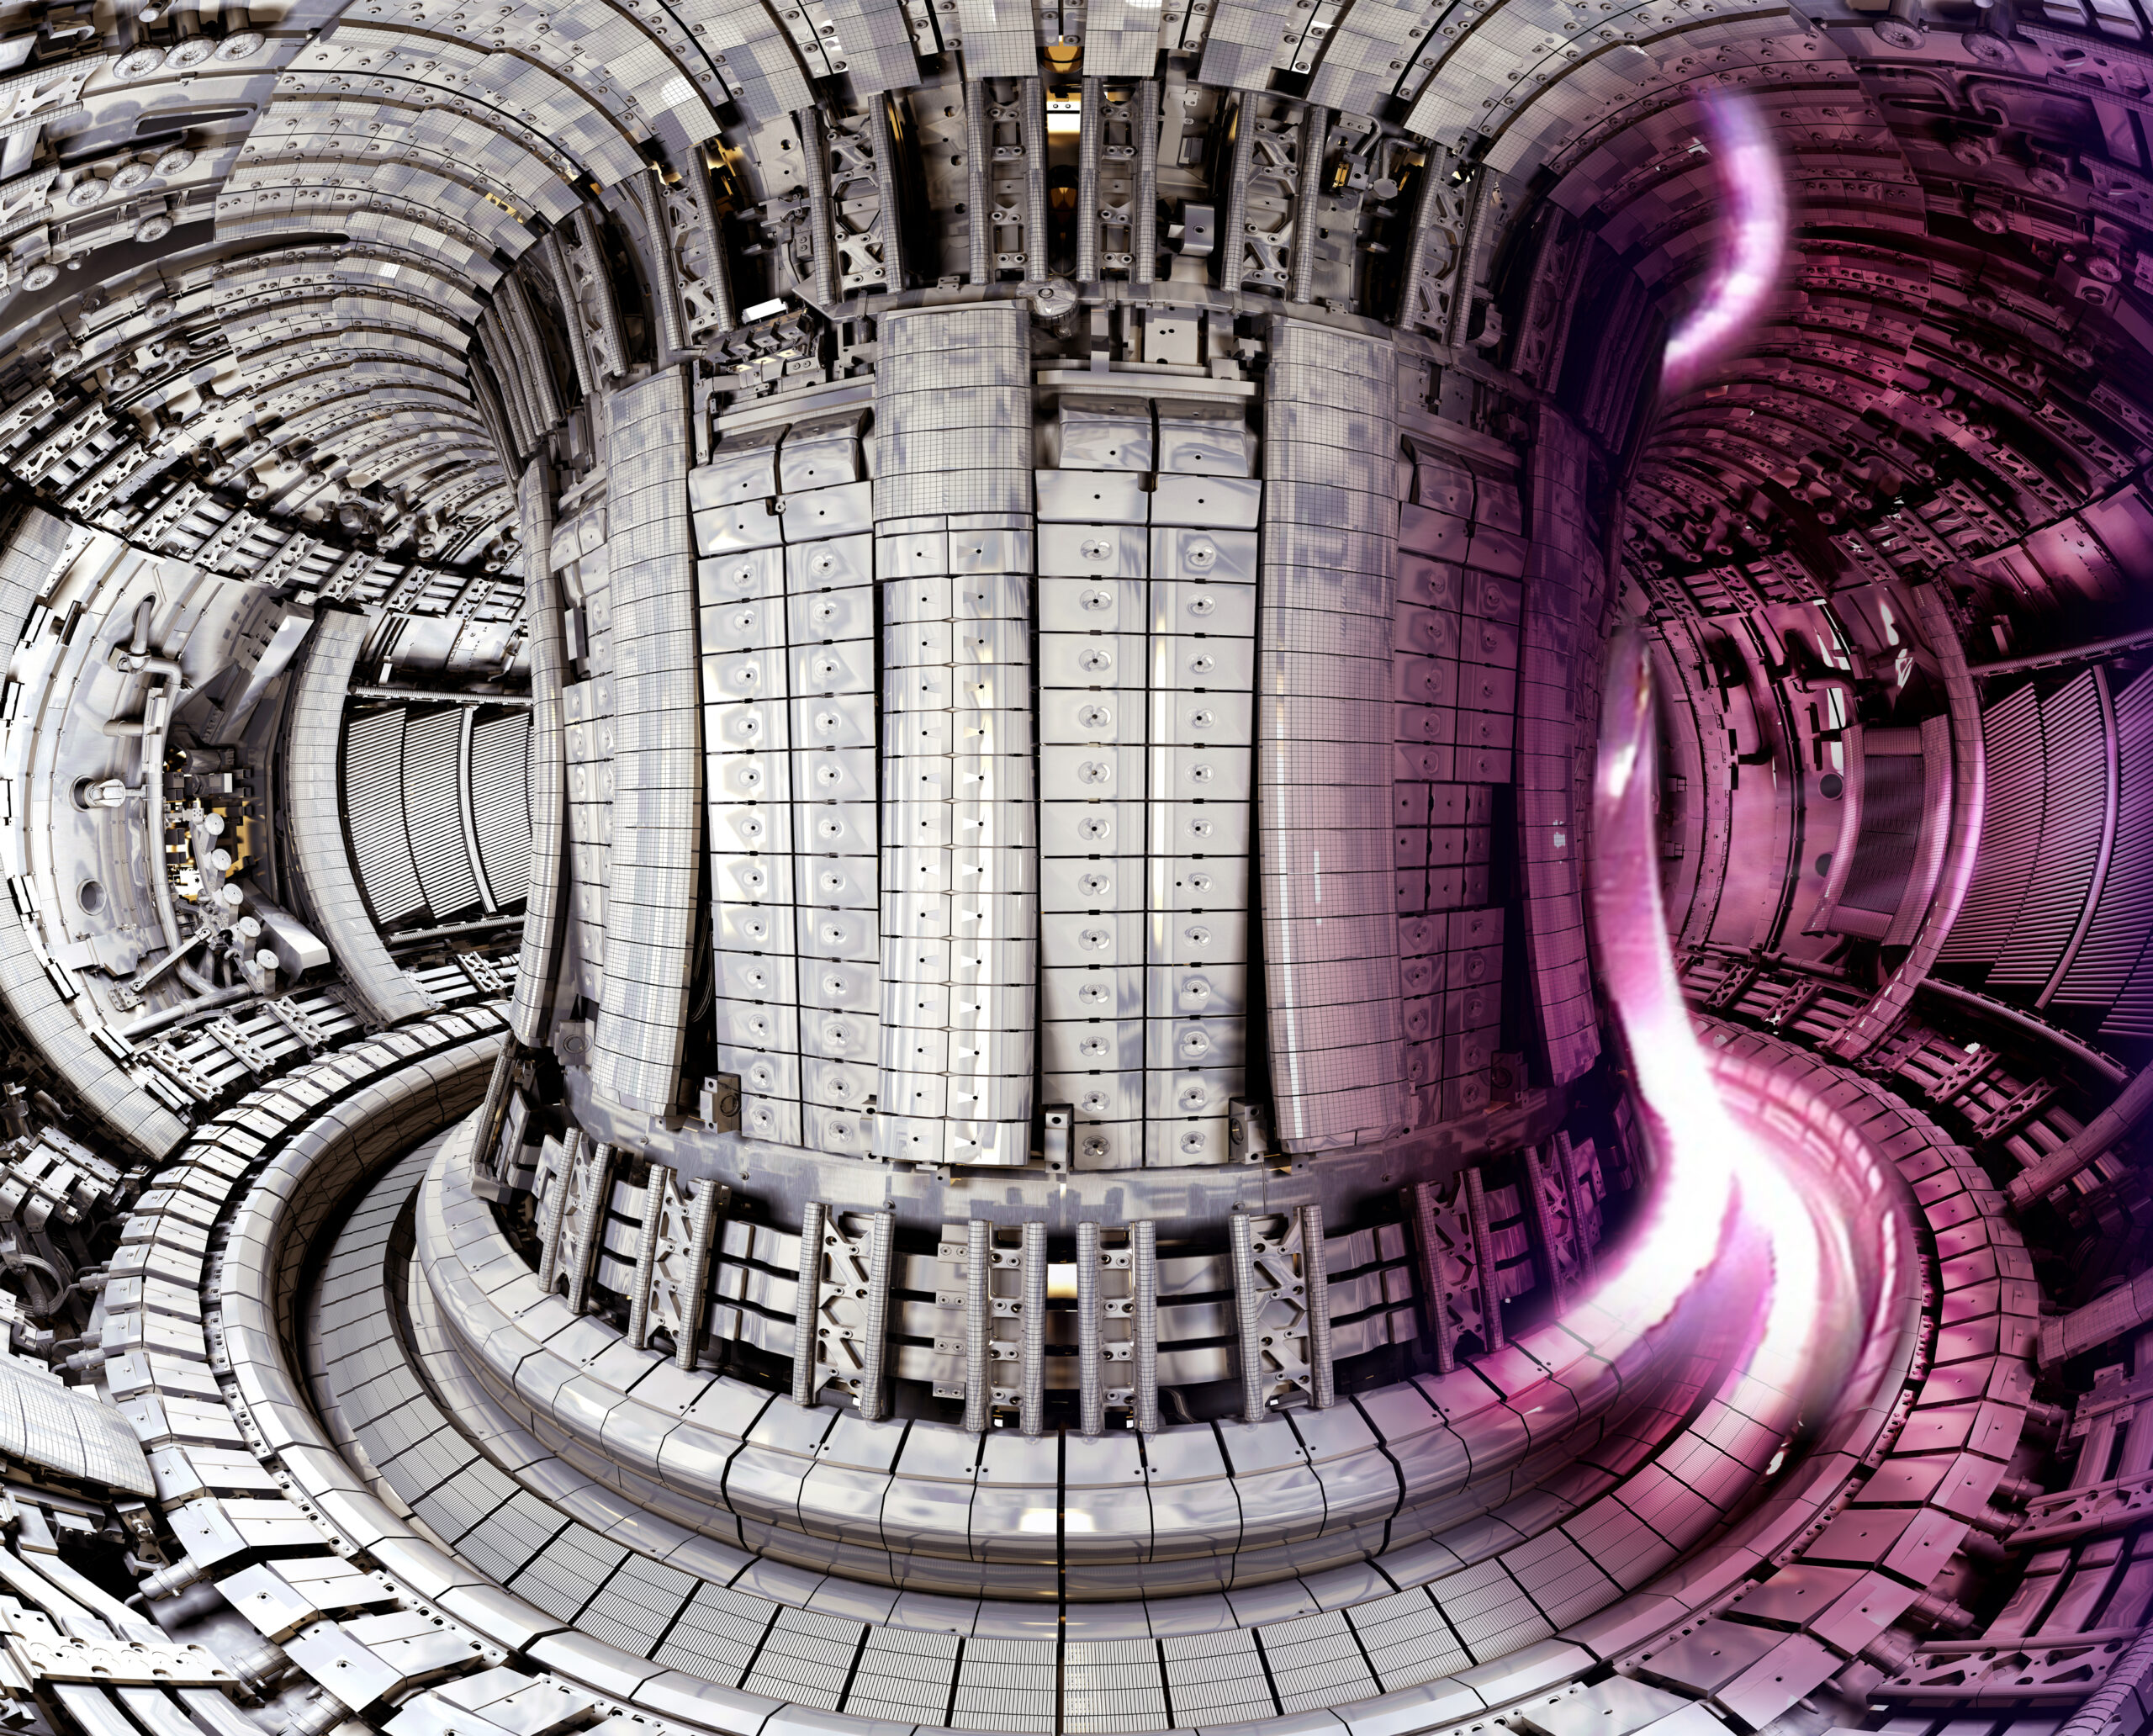
\includegraphics[width = 0.8\textwidth]{0 - introduction/images/JET.jpg}
        \caption{Illustration of the interior of the Joint European Torus (JET) reactor, located at the Culham Centre for Fusion Energy (CCFE). At the time of creation, JET was the largest tokamak in the world. (Source: CCFE)}
    \end{figure}

    The physical and numerical modeling of plasmas is a crucial area of study for tokamaks because it helps to understand and predict the behavior of the hot plasma in the containment vessel. The plasma must be maintained at high temperatures and densities in order to achieve fusion, and understanding its behavior is essential for optimizing the conditions in the tokamak and improving the fusion efficiency. Plasma modeling allows the simulation of various scenarios, such as changes in the magnetic fields or the heating methods used, and the observation of how these affects the plasma, allowing researchers and engineers to make informed decisions about how to increase the energy yield.
    
    In addition, plasma modeling helps to identify and resolve potential problems that may arise during the fusion reaction, such as instabilities in the plasma or unwanted interactions with the chamber walls. By using computer simulations, these issues can be identified and resolved before they occur outside of the simulation, making the process safer and more efficient.
    
    In this introduction, we present an overview of plasmas and their modeling, and the great difficulties these pose in tokamak-like environments.

    \BA{Need more references for the above paragraphs.}


    \documentclass[12pt, a4paper]{report}

\documentclass[12pt, a4paper]{report}

\documentclass[12pt, a4paper]{report}

\input{template/main.tex}

\title{\BA{Title in Progress...}}
\author{Boris Andrews}
\affil{Mathematical Institute, University of Oxford}
\date{\today}


\begin{document}
    \pagenumbering{gobble}
    \maketitle
    
    
    \begin{abstract}
        Magnetic confinement reactors---in particular tokamaks---offer one of the most promising options for achieving practical nuclear fusion, with the potential to provide virtually limitless, clean energy. The theoretical and numerical modeling of tokamak plasmas is simultaneously an essential component of effective reactor design, and a great research barrier. Tokamak operational conditions exhibit comparatively low Knudsen numbers. Kinetic effects, including kinetic waves and instabilities, Landau damping, bump-on-tail instabilities and more, are therefore highly influential in tokamak plasma dynamics. Purely fluid models are inherently incapable of capturing these effects, whereas the high dimensionality in purely kinetic models render them practically intractable for most relevant purposes.

        We consider a $\delta\!f$ decomposition model, with a macroscopic fluid background and microscopic kinetic correction, both fully coupled to each other. A similar manner of discretization is proposed to that used in the recent \texttt{STRUPHY} code \cite{Holderied_Possanner_Wang_2021, Holderied_2022, Li_et_al_2023} with a finite-element model for the background and a pseudo-particle/PiC model for the correction.

        The fluid background satisfies the full, non-linear, resistive, compressible, Hall MHD equations. \cite{Laakmann_Hu_Farrell_2022} introduces finite-element(-in-space) implicit timesteppers for the incompressible analogue to this system with structure-preserving (SP) properties in the ideal case, alongside parameter-robust preconditioners. We show that these timesteppers can derive from a finite-element-in-time (FET) (and finite-element-in-space) interpretation. The benefits of this reformulation are discussed, including the derivation of timesteppers that are higher order in time, and the quantifiable dissipative SP properties in the non-ideal, resistive case.
        
        We discuss possible options for extending this FET approach to timesteppers for the compressible case.

        The kinetic corrections satisfy linearized Boltzmann equations. Using a Lénard--Bernstein collision operator, these take Fokker--Planck-like forms \cite{Fokker_1914, Planck_1917} wherein pseudo-particles in the numerical model obey the neoclassical transport equations, with particle-independent Brownian drift terms. This offers a rigorous methodology for incorporating collisions into the particle transport model, without coupling the equations of motions for each particle.
        
        Works by Chen, Chacón et al. \cite{Chen_Chacón_Barnes_2011, Chacón_Chen_Barnes_2013, Chen_Chacón_2014, Chen_Chacón_2015} have developed structure-preserving particle pushers for neoclassical transport in the Vlasov equations, derived from Crank--Nicolson integrators. We show these too can can derive from a FET interpretation, similarly offering potential extensions to higher-order-in-time particle pushers. The FET formulation is used also to consider how the stochastic drift terms can be incorporated into the pushers. Stochastic gyrokinetic expansions are also discussed.

        Different options for the numerical implementation of these schemes are considered.

        Due to the efficacy of FET in the development of SP timesteppers for both the fluid and kinetic component, we hope this approach will prove effective in the future for developing SP timesteppers for the full hybrid model. We hope this will give us the opportunity to incorporate previously inaccessible kinetic effects into the highly effective, modern, finite-element MHD models.
    \end{abstract}
    
    
    \newpage
    \tableofcontents
    
    
    \newpage
    \pagenumbering{arabic}
    %\linenumbers\renewcommand\thelinenumber{\color{black!50}\arabic{linenumber}}
            \input{0 - introduction/main.tex}
        \part{Research}
            \input{1 - low-noise PiC models/main.tex}
            \input{2 - kinetic component/main.tex}
            \input{3 - fluid component/main.tex}
            \input{4 - numerical implementation/main.tex}
        \part{Project Overview}
            \input{5 - research plan/main.tex}
            \input{6 - summary/main.tex}
    
    
    %\section{}
    \newpage
    \pagenumbering{gobble}
        \printbibliography


    \newpage
    \pagenumbering{roman}
    \appendix
        \part{Appendices}
            \input{8 - Hilbert complexes/main.tex}
            \input{9 - weak conservation proofs/main.tex}
\end{document}


\title{\BA{Title in Progress...}}
\author{Boris Andrews}
\affil{Mathematical Institute, University of Oxford}
\date{\today}


\begin{document}
    \pagenumbering{gobble}
    \maketitle
    
    
    \begin{abstract}
        Magnetic confinement reactors---in particular tokamaks---offer one of the most promising options for achieving practical nuclear fusion, with the potential to provide virtually limitless, clean energy. The theoretical and numerical modeling of tokamak plasmas is simultaneously an essential component of effective reactor design, and a great research barrier. Tokamak operational conditions exhibit comparatively low Knudsen numbers. Kinetic effects, including kinetic waves and instabilities, Landau damping, bump-on-tail instabilities and more, are therefore highly influential in tokamak plasma dynamics. Purely fluid models are inherently incapable of capturing these effects, whereas the high dimensionality in purely kinetic models render them practically intractable for most relevant purposes.

        We consider a $\delta\!f$ decomposition model, with a macroscopic fluid background and microscopic kinetic correction, both fully coupled to each other. A similar manner of discretization is proposed to that used in the recent \texttt{STRUPHY} code \cite{Holderied_Possanner_Wang_2021, Holderied_2022, Li_et_al_2023} with a finite-element model for the background and a pseudo-particle/PiC model for the correction.

        The fluid background satisfies the full, non-linear, resistive, compressible, Hall MHD equations. \cite{Laakmann_Hu_Farrell_2022} introduces finite-element(-in-space) implicit timesteppers for the incompressible analogue to this system with structure-preserving (SP) properties in the ideal case, alongside parameter-robust preconditioners. We show that these timesteppers can derive from a finite-element-in-time (FET) (and finite-element-in-space) interpretation. The benefits of this reformulation are discussed, including the derivation of timesteppers that are higher order in time, and the quantifiable dissipative SP properties in the non-ideal, resistive case.
        
        We discuss possible options for extending this FET approach to timesteppers for the compressible case.

        The kinetic corrections satisfy linearized Boltzmann equations. Using a Lénard--Bernstein collision operator, these take Fokker--Planck-like forms \cite{Fokker_1914, Planck_1917} wherein pseudo-particles in the numerical model obey the neoclassical transport equations, with particle-independent Brownian drift terms. This offers a rigorous methodology for incorporating collisions into the particle transport model, without coupling the equations of motions for each particle.
        
        Works by Chen, Chacón et al. \cite{Chen_Chacón_Barnes_2011, Chacón_Chen_Barnes_2013, Chen_Chacón_2014, Chen_Chacón_2015} have developed structure-preserving particle pushers for neoclassical transport in the Vlasov equations, derived from Crank--Nicolson integrators. We show these too can can derive from a FET interpretation, similarly offering potential extensions to higher-order-in-time particle pushers. The FET formulation is used also to consider how the stochastic drift terms can be incorporated into the pushers. Stochastic gyrokinetic expansions are also discussed.

        Different options for the numerical implementation of these schemes are considered.

        Due to the efficacy of FET in the development of SP timesteppers for both the fluid and kinetic component, we hope this approach will prove effective in the future for developing SP timesteppers for the full hybrid model. We hope this will give us the opportunity to incorporate previously inaccessible kinetic effects into the highly effective, modern, finite-element MHD models.
    \end{abstract}
    
    
    \newpage
    \tableofcontents
    
    
    \newpage
    \pagenumbering{arabic}
    %\linenumbers\renewcommand\thelinenumber{\color{black!50}\arabic{linenumber}}
            \documentclass[12pt, a4paper]{report}

\input{template/main.tex}

\title{\BA{Title in Progress...}}
\author{Boris Andrews}
\affil{Mathematical Institute, University of Oxford}
\date{\today}


\begin{document}
    \pagenumbering{gobble}
    \maketitle
    
    
    \begin{abstract}
        Magnetic confinement reactors---in particular tokamaks---offer one of the most promising options for achieving practical nuclear fusion, with the potential to provide virtually limitless, clean energy. The theoretical and numerical modeling of tokamak plasmas is simultaneously an essential component of effective reactor design, and a great research barrier. Tokamak operational conditions exhibit comparatively low Knudsen numbers. Kinetic effects, including kinetic waves and instabilities, Landau damping, bump-on-tail instabilities and more, are therefore highly influential in tokamak plasma dynamics. Purely fluid models are inherently incapable of capturing these effects, whereas the high dimensionality in purely kinetic models render them practically intractable for most relevant purposes.

        We consider a $\delta\!f$ decomposition model, with a macroscopic fluid background and microscopic kinetic correction, both fully coupled to each other. A similar manner of discretization is proposed to that used in the recent \texttt{STRUPHY} code \cite{Holderied_Possanner_Wang_2021, Holderied_2022, Li_et_al_2023} with a finite-element model for the background and a pseudo-particle/PiC model for the correction.

        The fluid background satisfies the full, non-linear, resistive, compressible, Hall MHD equations. \cite{Laakmann_Hu_Farrell_2022} introduces finite-element(-in-space) implicit timesteppers for the incompressible analogue to this system with structure-preserving (SP) properties in the ideal case, alongside parameter-robust preconditioners. We show that these timesteppers can derive from a finite-element-in-time (FET) (and finite-element-in-space) interpretation. The benefits of this reformulation are discussed, including the derivation of timesteppers that are higher order in time, and the quantifiable dissipative SP properties in the non-ideal, resistive case.
        
        We discuss possible options for extending this FET approach to timesteppers for the compressible case.

        The kinetic corrections satisfy linearized Boltzmann equations. Using a Lénard--Bernstein collision operator, these take Fokker--Planck-like forms \cite{Fokker_1914, Planck_1917} wherein pseudo-particles in the numerical model obey the neoclassical transport equations, with particle-independent Brownian drift terms. This offers a rigorous methodology for incorporating collisions into the particle transport model, without coupling the equations of motions for each particle.
        
        Works by Chen, Chacón et al. \cite{Chen_Chacón_Barnes_2011, Chacón_Chen_Barnes_2013, Chen_Chacón_2014, Chen_Chacón_2015} have developed structure-preserving particle pushers for neoclassical transport in the Vlasov equations, derived from Crank--Nicolson integrators. We show these too can can derive from a FET interpretation, similarly offering potential extensions to higher-order-in-time particle pushers. The FET formulation is used also to consider how the stochastic drift terms can be incorporated into the pushers. Stochastic gyrokinetic expansions are also discussed.

        Different options for the numerical implementation of these schemes are considered.

        Due to the efficacy of FET in the development of SP timesteppers for both the fluid and kinetic component, we hope this approach will prove effective in the future for developing SP timesteppers for the full hybrid model. We hope this will give us the opportunity to incorporate previously inaccessible kinetic effects into the highly effective, modern, finite-element MHD models.
    \end{abstract}
    
    
    \newpage
    \tableofcontents
    
    
    \newpage
    \pagenumbering{arabic}
    %\linenumbers\renewcommand\thelinenumber{\color{black!50}\arabic{linenumber}}
            \input{0 - introduction/main.tex}
        \part{Research}
            \input{1 - low-noise PiC models/main.tex}
            \input{2 - kinetic component/main.tex}
            \input{3 - fluid component/main.tex}
            \input{4 - numerical implementation/main.tex}
        \part{Project Overview}
            \input{5 - research plan/main.tex}
            \input{6 - summary/main.tex}
    
    
    %\section{}
    \newpage
    \pagenumbering{gobble}
        \printbibliography


    \newpage
    \pagenumbering{roman}
    \appendix
        \part{Appendices}
            \input{8 - Hilbert complexes/main.tex}
            \input{9 - weak conservation proofs/main.tex}
\end{document}

        \part{Research}
            \documentclass[12pt, a4paper]{report}

\input{template/main.tex}

\title{\BA{Title in Progress...}}
\author{Boris Andrews}
\affil{Mathematical Institute, University of Oxford}
\date{\today}


\begin{document}
    \pagenumbering{gobble}
    \maketitle
    
    
    \begin{abstract}
        Magnetic confinement reactors---in particular tokamaks---offer one of the most promising options for achieving practical nuclear fusion, with the potential to provide virtually limitless, clean energy. The theoretical and numerical modeling of tokamak plasmas is simultaneously an essential component of effective reactor design, and a great research barrier. Tokamak operational conditions exhibit comparatively low Knudsen numbers. Kinetic effects, including kinetic waves and instabilities, Landau damping, bump-on-tail instabilities and more, are therefore highly influential in tokamak plasma dynamics. Purely fluid models are inherently incapable of capturing these effects, whereas the high dimensionality in purely kinetic models render them practically intractable for most relevant purposes.

        We consider a $\delta\!f$ decomposition model, with a macroscopic fluid background and microscopic kinetic correction, both fully coupled to each other. A similar manner of discretization is proposed to that used in the recent \texttt{STRUPHY} code \cite{Holderied_Possanner_Wang_2021, Holderied_2022, Li_et_al_2023} with a finite-element model for the background and a pseudo-particle/PiC model for the correction.

        The fluid background satisfies the full, non-linear, resistive, compressible, Hall MHD equations. \cite{Laakmann_Hu_Farrell_2022} introduces finite-element(-in-space) implicit timesteppers for the incompressible analogue to this system with structure-preserving (SP) properties in the ideal case, alongside parameter-robust preconditioners. We show that these timesteppers can derive from a finite-element-in-time (FET) (and finite-element-in-space) interpretation. The benefits of this reformulation are discussed, including the derivation of timesteppers that are higher order in time, and the quantifiable dissipative SP properties in the non-ideal, resistive case.
        
        We discuss possible options for extending this FET approach to timesteppers for the compressible case.

        The kinetic corrections satisfy linearized Boltzmann equations. Using a Lénard--Bernstein collision operator, these take Fokker--Planck-like forms \cite{Fokker_1914, Planck_1917} wherein pseudo-particles in the numerical model obey the neoclassical transport equations, with particle-independent Brownian drift terms. This offers a rigorous methodology for incorporating collisions into the particle transport model, without coupling the equations of motions for each particle.
        
        Works by Chen, Chacón et al. \cite{Chen_Chacón_Barnes_2011, Chacón_Chen_Barnes_2013, Chen_Chacón_2014, Chen_Chacón_2015} have developed structure-preserving particle pushers for neoclassical transport in the Vlasov equations, derived from Crank--Nicolson integrators. We show these too can can derive from a FET interpretation, similarly offering potential extensions to higher-order-in-time particle pushers. The FET formulation is used also to consider how the stochastic drift terms can be incorporated into the pushers. Stochastic gyrokinetic expansions are also discussed.

        Different options for the numerical implementation of these schemes are considered.

        Due to the efficacy of FET in the development of SP timesteppers for both the fluid and kinetic component, we hope this approach will prove effective in the future for developing SP timesteppers for the full hybrid model. We hope this will give us the opportunity to incorporate previously inaccessible kinetic effects into the highly effective, modern, finite-element MHD models.
    \end{abstract}
    
    
    \newpage
    \tableofcontents
    
    
    \newpage
    \pagenumbering{arabic}
    %\linenumbers\renewcommand\thelinenumber{\color{black!50}\arabic{linenumber}}
            \input{0 - introduction/main.tex}
        \part{Research}
            \input{1 - low-noise PiC models/main.tex}
            \input{2 - kinetic component/main.tex}
            \input{3 - fluid component/main.tex}
            \input{4 - numerical implementation/main.tex}
        \part{Project Overview}
            \input{5 - research plan/main.tex}
            \input{6 - summary/main.tex}
    
    
    %\section{}
    \newpage
    \pagenumbering{gobble}
        \printbibliography


    \newpage
    \pagenumbering{roman}
    \appendix
        \part{Appendices}
            \input{8 - Hilbert complexes/main.tex}
            \input{9 - weak conservation proofs/main.tex}
\end{document}

            \documentclass[12pt, a4paper]{report}

\input{template/main.tex}

\title{\BA{Title in Progress...}}
\author{Boris Andrews}
\affil{Mathematical Institute, University of Oxford}
\date{\today}


\begin{document}
    \pagenumbering{gobble}
    \maketitle
    
    
    \begin{abstract}
        Magnetic confinement reactors---in particular tokamaks---offer one of the most promising options for achieving practical nuclear fusion, with the potential to provide virtually limitless, clean energy. The theoretical and numerical modeling of tokamak plasmas is simultaneously an essential component of effective reactor design, and a great research barrier. Tokamak operational conditions exhibit comparatively low Knudsen numbers. Kinetic effects, including kinetic waves and instabilities, Landau damping, bump-on-tail instabilities and more, are therefore highly influential in tokamak plasma dynamics. Purely fluid models are inherently incapable of capturing these effects, whereas the high dimensionality in purely kinetic models render them practically intractable for most relevant purposes.

        We consider a $\delta\!f$ decomposition model, with a macroscopic fluid background and microscopic kinetic correction, both fully coupled to each other. A similar manner of discretization is proposed to that used in the recent \texttt{STRUPHY} code \cite{Holderied_Possanner_Wang_2021, Holderied_2022, Li_et_al_2023} with a finite-element model for the background and a pseudo-particle/PiC model for the correction.

        The fluid background satisfies the full, non-linear, resistive, compressible, Hall MHD equations. \cite{Laakmann_Hu_Farrell_2022} introduces finite-element(-in-space) implicit timesteppers for the incompressible analogue to this system with structure-preserving (SP) properties in the ideal case, alongside parameter-robust preconditioners. We show that these timesteppers can derive from a finite-element-in-time (FET) (and finite-element-in-space) interpretation. The benefits of this reformulation are discussed, including the derivation of timesteppers that are higher order in time, and the quantifiable dissipative SP properties in the non-ideal, resistive case.
        
        We discuss possible options for extending this FET approach to timesteppers for the compressible case.

        The kinetic corrections satisfy linearized Boltzmann equations. Using a Lénard--Bernstein collision operator, these take Fokker--Planck-like forms \cite{Fokker_1914, Planck_1917} wherein pseudo-particles in the numerical model obey the neoclassical transport equations, with particle-independent Brownian drift terms. This offers a rigorous methodology for incorporating collisions into the particle transport model, without coupling the equations of motions for each particle.
        
        Works by Chen, Chacón et al. \cite{Chen_Chacón_Barnes_2011, Chacón_Chen_Barnes_2013, Chen_Chacón_2014, Chen_Chacón_2015} have developed structure-preserving particle pushers for neoclassical transport in the Vlasov equations, derived from Crank--Nicolson integrators. We show these too can can derive from a FET interpretation, similarly offering potential extensions to higher-order-in-time particle pushers. The FET formulation is used also to consider how the stochastic drift terms can be incorporated into the pushers. Stochastic gyrokinetic expansions are also discussed.

        Different options for the numerical implementation of these schemes are considered.

        Due to the efficacy of FET in the development of SP timesteppers for both the fluid and kinetic component, we hope this approach will prove effective in the future for developing SP timesteppers for the full hybrid model. We hope this will give us the opportunity to incorporate previously inaccessible kinetic effects into the highly effective, modern, finite-element MHD models.
    \end{abstract}
    
    
    \newpage
    \tableofcontents
    
    
    \newpage
    \pagenumbering{arabic}
    %\linenumbers\renewcommand\thelinenumber{\color{black!50}\arabic{linenumber}}
            \input{0 - introduction/main.tex}
        \part{Research}
            \input{1 - low-noise PiC models/main.tex}
            \input{2 - kinetic component/main.tex}
            \input{3 - fluid component/main.tex}
            \input{4 - numerical implementation/main.tex}
        \part{Project Overview}
            \input{5 - research plan/main.tex}
            \input{6 - summary/main.tex}
    
    
    %\section{}
    \newpage
    \pagenumbering{gobble}
        \printbibliography


    \newpage
    \pagenumbering{roman}
    \appendix
        \part{Appendices}
            \input{8 - Hilbert complexes/main.tex}
            \input{9 - weak conservation proofs/main.tex}
\end{document}

            \documentclass[12pt, a4paper]{report}

\input{template/main.tex}

\title{\BA{Title in Progress...}}
\author{Boris Andrews}
\affil{Mathematical Institute, University of Oxford}
\date{\today}


\begin{document}
    \pagenumbering{gobble}
    \maketitle
    
    
    \begin{abstract}
        Magnetic confinement reactors---in particular tokamaks---offer one of the most promising options for achieving practical nuclear fusion, with the potential to provide virtually limitless, clean energy. The theoretical and numerical modeling of tokamak plasmas is simultaneously an essential component of effective reactor design, and a great research barrier. Tokamak operational conditions exhibit comparatively low Knudsen numbers. Kinetic effects, including kinetic waves and instabilities, Landau damping, bump-on-tail instabilities and more, are therefore highly influential in tokamak plasma dynamics. Purely fluid models are inherently incapable of capturing these effects, whereas the high dimensionality in purely kinetic models render them practically intractable for most relevant purposes.

        We consider a $\delta\!f$ decomposition model, with a macroscopic fluid background and microscopic kinetic correction, both fully coupled to each other. A similar manner of discretization is proposed to that used in the recent \texttt{STRUPHY} code \cite{Holderied_Possanner_Wang_2021, Holderied_2022, Li_et_al_2023} with a finite-element model for the background and a pseudo-particle/PiC model for the correction.

        The fluid background satisfies the full, non-linear, resistive, compressible, Hall MHD equations. \cite{Laakmann_Hu_Farrell_2022} introduces finite-element(-in-space) implicit timesteppers for the incompressible analogue to this system with structure-preserving (SP) properties in the ideal case, alongside parameter-robust preconditioners. We show that these timesteppers can derive from a finite-element-in-time (FET) (and finite-element-in-space) interpretation. The benefits of this reformulation are discussed, including the derivation of timesteppers that are higher order in time, and the quantifiable dissipative SP properties in the non-ideal, resistive case.
        
        We discuss possible options for extending this FET approach to timesteppers for the compressible case.

        The kinetic corrections satisfy linearized Boltzmann equations. Using a Lénard--Bernstein collision operator, these take Fokker--Planck-like forms \cite{Fokker_1914, Planck_1917} wherein pseudo-particles in the numerical model obey the neoclassical transport equations, with particle-independent Brownian drift terms. This offers a rigorous methodology for incorporating collisions into the particle transport model, without coupling the equations of motions for each particle.
        
        Works by Chen, Chacón et al. \cite{Chen_Chacón_Barnes_2011, Chacón_Chen_Barnes_2013, Chen_Chacón_2014, Chen_Chacón_2015} have developed structure-preserving particle pushers for neoclassical transport in the Vlasov equations, derived from Crank--Nicolson integrators. We show these too can can derive from a FET interpretation, similarly offering potential extensions to higher-order-in-time particle pushers. The FET formulation is used also to consider how the stochastic drift terms can be incorporated into the pushers. Stochastic gyrokinetic expansions are also discussed.

        Different options for the numerical implementation of these schemes are considered.

        Due to the efficacy of FET in the development of SP timesteppers for both the fluid and kinetic component, we hope this approach will prove effective in the future for developing SP timesteppers for the full hybrid model. We hope this will give us the opportunity to incorporate previously inaccessible kinetic effects into the highly effective, modern, finite-element MHD models.
    \end{abstract}
    
    
    \newpage
    \tableofcontents
    
    
    \newpage
    \pagenumbering{arabic}
    %\linenumbers\renewcommand\thelinenumber{\color{black!50}\arabic{linenumber}}
            \input{0 - introduction/main.tex}
        \part{Research}
            \input{1 - low-noise PiC models/main.tex}
            \input{2 - kinetic component/main.tex}
            \input{3 - fluid component/main.tex}
            \input{4 - numerical implementation/main.tex}
        \part{Project Overview}
            \input{5 - research plan/main.tex}
            \input{6 - summary/main.tex}
    
    
    %\section{}
    \newpage
    \pagenumbering{gobble}
        \printbibliography


    \newpage
    \pagenumbering{roman}
    \appendix
        \part{Appendices}
            \input{8 - Hilbert complexes/main.tex}
            \input{9 - weak conservation proofs/main.tex}
\end{document}

            \documentclass[12pt, a4paper]{report}

\input{template/main.tex}

\title{\BA{Title in Progress...}}
\author{Boris Andrews}
\affil{Mathematical Institute, University of Oxford}
\date{\today}


\begin{document}
    \pagenumbering{gobble}
    \maketitle
    
    
    \begin{abstract}
        Magnetic confinement reactors---in particular tokamaks---offer one of the most promising options for achieving practical nuclear fusion, with the potential to provide virtually limitless, clean energy. The theoretical and numerical modeling of tokamak plasmas is simultaneously an essential component of effective reactor design, and a great research barrier. Tokamak operational conditions exhibit comparatively low Knudsen numbers. Kinetic effects, including kinetic waves and instabilities, Landau damping, bump-on-tail instabilities and more, are therefore highly influential in tokamak plasma dynamics. Purely fluid models are inherently incapable of capturing these effects, whereas the high dimensionality in purely kinetic models render them practically intractable for most relevant purposes.

        We consider a $\delta\!f$ decomposition model, with a macroscopic fluid background and microscopic kinetic correction, both fully coupled to each other. A similar manner of discretization is proposed to that used in the recent \texttt{STRUPHY} code \cite{Holderied_Possanner_Wang_2021, Holderied_2022, Li_et_al_2023} with a finite-element model for the background and a pseudo-particle/PiC model for the correction.

        The fluid background satisfies the full, non-linear, resistive, compressible, Hall MHD equations. \cite{Laakmann_Hu_Farrell_2022} introduces finite-element(-in-space) implicit timesteppers for the incompressible analogue to this system with structure-preserving (SP) properties in the ideal case, alongside parameter-robust preconditioners. We show that these timesteppers can derive from a finite-element-in-time (FET) (and finite-element-in-space) interpretation. The benefits of this reformulation are discussed, including the derivation of timesteppers that are higher order in time, and the quantifiable dissipative SP properties in the non-ideal, resistive case.
        
        We discuss possible options for extending this FET approach to timesteppers for the compressible case.

        The kinetic corrections satisfy linearized Boltzmann equations. Using a Lénard--Bernstein collision operator, these take Fokker--Planck-like forms \cite{Fokker_1914, Planck_1917} wherein pseudo-particles in the numerical model obey the neoclassical transport equations, with particle-independent Brownian drift terms. This offers a rigorous methodology for incorporating collisions into the particle transport model, without coupling the equations of motions for each particle.
        
        Works by Chen, Chacón et al. \cite{Chen_Chacón_Barnes_2011, Chacón_Chen_Barnes_2013, Chen_Chacón_2014, Chen_Chacón_2015} have developed structure-preserving particle pushers for neoclassical transport in the Vlasov equations, derived from Crank--Nicolson integrators. We show these too can can derive from a FET interpretation, similarly offering potential extensions to higher-order-in-time particle pushers. The FET formulation is used also to consider how the stochastic drift terms can be incorporated into the pushers. Stochastic gyrokinetic expansions are also discussed.

        Different options for the numerical implementation of these schemes are considered.

        Due to the efficacy of FET in the development of SP timesteppers for both the fluid and kinetic component, we hope this approach will prove effective in the future for developing SP timesteppers for the full hybrid model. We hope this will give us the opportunity to incorporate previously inaccessible kinetic effects into the highly effective, modern, finite-element MHD models.
    \end{abstract}
    
    
    \newpage
    \tableofcontents
    
    
    \newpage
    \pagenumbering{arabic}
    %\linenumbers\renewcommand\thelinenumber{\color{black!50}\arabic{linenumber}}
            \input{0 - introduction/main.tex}
        \part{Research}
            \input{1 - low-noise PiC models/main.tex}
            \input{2 - kinetic component/main.tex}
            \input{3 - fluid component/main.tex}
            \input{4 - numerical implementation/main.tex}
        \part{Project Overview}
            \input{5 - research plan/main.tex}
            \input{6 - summary/main.tex}
    
    
    %\section{}
    \newpage
    \pagenumbering{gobble}
        \printbibliography


    \newpage
    \pagenumbering{roman}
    \appendix
        \part{Appendices}
            \input{8 - Hilbert complexes/main.tex}
            \input{9 - weak conservation proofs/main.tex}
\end{document}

        \part{Project Overview}
            \documentclass[12pt, a4paper]{report}

\input{template/main.tex}

\title{\BA{Title in Progress...}}
\author{Boris Andrews}
\affil{Mathematical Institute, University of Oxford}
\date{\today}


\begin{document}
    \pagenumbering{gobble}
    \maketitle
    
    
    \begin{abstract}
        Magnetic confinement reactors---in particular tokamaks---offer one of the most promising options for achieving practical nuclear fusion, with the potential to provide virtually limitless, clean energy. The theoretical and numerical modeling of tokamak plasmas is simultaneously an essential component of effective reactor design, and a great research barrier. Tokamak operational conditions exhibit comparatively low Knudsen numbers. Kinetic effects, including kinetic waves and instabilities, Landau damping, bump-on-tail instabilities and more, are therefore highly influential in tokamak plasma dynamics. Purely fluid models are inherently incapable of capturing these effects, whereas the high dimensionality in purely kinetic models render them practically intractable for most relevant purposes.

        We consider a $\delta\!f$ decomposition model, with a macroscopic fluid background and microscopic kinetic correction, both fully coupled to each other. A similar manner of discretization is proposed to that used in the recent \texttt{STRUPHY} code \cite{Holderied_Possanner_Wang_2021, Holderied_2022, Li_et_al_2023} with a finite-element model for the background and a pseudo-particle/PiC model for the correction.

        The fluid background satisfies the full, non-linear, resistive, compressible, Hall MHD equations. \cite{Laakmann_Hu_Farrell_2022} introduces finite-element(-in-space) implicit timesteppers for the incompressible analogue to this system with structure-preserving (SP) properties in the ideal case, alongside parameter-robust preconditioners. We show that these timesteppers can derive from a finite-element-in-time (FET) (and finite-element-in-space) interpretation. The benefits of this reformulation are discussed, including the derivation of timesteppers that are higher order in time, and the quantifiable dissipative SP properties in the non-ideal, resistive case.
        
        We discuss possible options for extending this FET approach to timesteppers for the compressible case.

        The kinetic corrections satisfy linearized Boltzmann equations. Using a Lénard--Bernstein collision operator, these take Fokker--Planck-like forms \cite{Fokker_1914, Planck_1917} wherein pseudo-particles in the numerical model obey the neoclassical transport equations, with particle-independent Brownian drift terms. This offers a rigorous methodology for incorporating collisions into the particle transport model, without coupling the equations of motions for each particle.
        
        Works by Chen, Chacón et al. \cite{Chen_Chacón_Barnes_2011, Chacón_Chen_Barnes_2013, Chen_Chacón_2014, Chen_Chacón_2015} have developed structure-preserving particle pushers for neoclassical transport in the Vlasov equations, derived from Crank--Nicolson integrators. We show these too can can derive from a FET interpretation, similarly offering potential extensions to higher-order-in-time particle pushers. The FET formulation is used also to consider how the stochastic drift terms can be incorporated into the pushers. Stochastic gyrokinetic expansions are also discussed.

        Different options for the numerical implementation of these schemes are considered.

        Due to the efficacy of FET in the development of SP timesteppers for both the fluid and kinetic component, we hope this approach will prove effective in the future for developing SP timesteppers for the full hybrid model. We hope this will give us the opportunity to incorporate previously inaccessible kinetic effects into the highly effective, modern, finite-element MHD models.
    \end{abstract}
    
    
    \newpage
    \tableofcontents
    
    
    \newpage
    \pagenumbering{arabic}
    %\linenumbers\renewcommand\thelinenumber{\color{black!50}\arabic{linenumber}}
            \input{0 - introduction/main.tex}
        \part{Research}
            \input{1 - low-noise PiC models/main.tex}
            \input{2 - kinetic component/main.tex}
            \input{3 - fluid component/main.tex}
            \input{4 - numerical implementation/main.tex}
        \part{Project Overview}
            \input{5 - research plan/main.tex}
            \input{6 - summary/main.tex}
    
    
    %\section{}
    \newpage
    \pagenumbering{gobble}
        \printbibliography


    \newpage
    \pagenumbering{roman}
    \appendix
        \part{Appendices}
            \input{8 - Hilbert complexes/main.tex}
            \input{9 - weak conservation proofs/main.tex}
\end{document}

            \documentclass[12pt, a4paper]{report}

\input{template/main.tex}

\title{\BA{Title in Progress...}}
\author{Boris Andrews}
\affil{Mathematical Institute, University of Oxford}
\date{\today}


\begin{document}
    \pagenumbering{gobble}
    \maketitle
    
    
    \begin{abstract}
        Magnetic confinement reactors---in particular tokamaks---offer one of the most promising options for achieving practical nuclear fusion, with the potential to provide virtually limitless, clean energy. The theoretical and numerical modeling of tokamak plasmas is simultaneously an essential component of effective reactor design, and a great research barrier. Tokamak operational conditions exhibit comparatively low Knudsen numbers. Kinetic effects, including kinetic waves and instabilities, Landau damping, bump-on-tail instabilities and more, are therefore highly influential in tokamak plasma dynamics. Purely fluid models are inherently incapable of capturing these effects, whereas the high dimensionality in purely kinetic models render them practically intractable for most relevant purposes.

        We consider a $\delta\!f$ decomposition model, with a macroscopic fluid background and microscopic kinetic correction, both fully coupled to each other. A similar manner of discretization is proposed to that used in the recent \texttt{STRUPHY} code \cite{Holderied_Possanner_Wang_2021, Holderied_2022, Li_et_al_2023} with a finite-element model for the background and a pseudo-particle/PiC model for the correction.

        The fluid background satisfies the full, non-linear, resistive, compressible, Hall MHD equations. \cite{Laakmann_Hu_Farrell_2022} introduces finite-element(-in-space) implicit timesteppers for the incompressible analogue to this system with structure-preserving (SP) properties in the ideal case, alongside parameter-robust preconditioners. We show that these timesteppers can derive from a finite-element-in-time (FET) (and finite-element-in-space) interpretation. The benefits of this reformulation are discussed, including the derivation of timesteppers that are higher order in time, and the quantifiable dissipative SP properties in the non-ideal, resistive case.
        
        We discuss possible options for extending this FET approach to timesteppers for the compressible case.

        The kinetic corrections satisfy linearized Boltzmann equations. Using a Lénard--Bernstein collision operator, these take Fokker--Planck-like forms \cite{Fokker_1914, Planck_1917} wherein pseudo-particles in the numerical model obey the neoclassical transport equations, with particle-independent Brownian drift terms. This offers a rigorous methodology for incorporating collisions into the particle transport model, without coupling the equations of motions for each particle.
        
        Works by Chen, Chacón et al. \cite{Chen_Chacón_Barnes_2011, Chacón_Chen_Barnes_2013, Chen_Chacón_2014, Chen_Chacón_2015} have developed structure-preserving particle pushers for neoclassical transport in the Vlasov equations, derived from Crank--Nicolson integrators. We show these too can can derive from a FET interpretation, similarly offering potential extensions to higher-order-in-time particle pushers. The FET formulation is used also to consider how the stochastic drift terms can be incorporated into the pushers. Stochastic gyrokinetic expansions are also discussed.

        Different options for the numerical implementation of these schemes are considered.

        Due to the efficacy of FET in the development of SP timesteppers for both the fluid and kinetic component, we hope this approach will prove effective in the future for developing SP timesteppers for the full hybrid model. We hope this will give us the opportunity to incorporate previously inaccessible kinetic effects into the highly effective, modern, finite-element MHD models.
    \end{abstract}
    
    
    \newpage
    \tableofcontents
    
    
    \newpage
    \pagenumbering{arabic}
    %\linenumbers\renewcommand\thelinenumber{\color{black!50}\arabic{linenumber}}
            \input{0 - introduction/main.tex}
        \part{Research}
            \input{1 - low-noise PiC models/main.tex}
            \input{2 - kinetic component/main.tex}
            \input{3 - fluid component/main.tex}
            \input{4 - numerical implementation/main.tex}
        \part{Project Overview}
            \input{5 - research plan/main.tex}
            \input{6 - summary/main.tex}
    
    
    %\section{}
    \newpage
    \pagenumbering{gobble}
        \printbibliography


    \newpage
    \pagenumbering{roman}
    \appendix
        \part{Appendices}
            \input{8 - Hilbert complexes/main.tex}
            \input{9 - weak conservation proofs/main.tex}
\end{document}

    
    
    %\section{}
    \newpage
    \pagenumbering{gobble}
        \printbibliography


    \newpage
    \pagenumbering{roman}
    \appendix
        \part{Appendices}
            \documentclass[12pt, a4paper]{report}

\input{template/main.tex}

\title{\BA{Title in Progress...}}
\author{Boris Andrews}
\affil{Mathematical Institute, University of Oxford}
\date{\today}


\begin{document}
    \pagenumbering{gobble}
    \maketitle
    
    
    \begin{abstract}
        Magnetic confinement reactors---in particular tokamaks---offer one of the most promising options for achieving practical nuclear fusion, with the potential to provide virtually limitless, clean energy. The theoretical and numerical modeling of tokamak plasmas is simultaneously an essential component of effective reactor design, and a great research barrier. Tokamak operational conditions exhibit comparatively low Knudsen numbers. Kinetic effects, including kinetic waves and instabilities, Landau damping, bump-on-tail instabilities and more, are therefore highly influential in tokamak plasma dynamics. Purely fluid models are inherently incapable of capturing these effects, whereas the high dimensionality in purely kinetic models render them practically intractable for most relevant purposes.

        We consider a $\delta\!f$ decomposition model, with a macroscopic fluid background and microscopic kinetic correction, both fully coupled to each other. A similar manner of discretization is proposed to that used in the recent \texttt{STRUPHY} code \cite{Holderied_Possanner_Wang_2021, Holderied_2022, Li_et_al_2023} with a finite-element model for the background and a pseudo-particle/PiC model for the correction.

        The fluid background satisfies the full, non-linear, resistive, compressible, Hall MHD equations. \cite{Laakmann_Hu_Farrell_2022} introduces finite-element(-in-space) implicit timesteppers for the incompressible analogue to this system with structure-preserving (SP) properties in the ideal case, alongside parameter-robust preconditioners. We show that these timesteppers can derive from a finite-element-in-time (FET) (and finite-element-in-space) interpretation. The benefits of this reformulation are discussed, including the derivation of timesteppers that are higher order in time, and the quantifiable dissipative SP properties in the non-ideal, resistive case.
        
        We discuss possible options for extending this FET approach to timesteppers for the compressible case.

        The kinetic corrections satisfy linearized Boltzmann equations. Using a Lénard--Bernstein collision operator, these take Fokker--Planck-like forms \cite{Fokker_1914, Planck_1917} wherein pseudo-particles in the numerical model obey the neoclassical transport equations, with particle-independent Brownian drift terms. This offers a rigorous methodology for incorporating collisions into the particle transport model, without coupling the equations of motions for each particle.
        
        Works by Chen, Chacón et al. \cite{Chen_Chacón_Barnes_2011, Chacón_Chen_Barnes_2013, Chen_Chacón_2014, Chen_Chacón_2015} have developed structure-preserving particle pushers for neoclassical transport in the Vlasov equations, derived from Crank--Nicolson integrators. We show these too can can derive from a FET interpretation, similarly offering potential extensions to higher-order-in-time particle pushers. The FET formulation is used also to consider how the stochastic drift terms can be incorporated into the pushers. Stochastic gyrokinetic expansions are also discussed.

        Different options for the numerical implementation of these schemes are considered.

        Due to the efficacy of FET in the development of SP timesteppers for both the fluid and kinetic component, we hope this approach will prove effective in the future for developing SP timesteppers for the full hybrid model. We hope this will give us the opportunity to incorporate previously inaccessible kinetic effects into the highly effective, modern, finite-element MHD models.
    \end{abstract}
    
    
    \newpage
    \tableofcontents
    
    
    \newpage
    \pagenumbering{arabic}
    %\linenumbers\renewcommand\thelinenumber{\color{black!50}\arabic{linenumber}}
            \input{0 - introduction/main.tex}
        \part{Research}
            \input{1 - low-noise PiC models/main.tex}
            \input{2 - kinetic component/main.tex}
            \input{3 - fluid component/main.tex}
            \input{4 - numerical implementation/main.tex}
        \part{Project Overview}
            \input{5 - research plan/main.tex}
            \input{6 - summary/main.tex}
    
    
    %\section{}
    \newpage
    \pagenumbering{gobble}
        \printbibliography


    \newpage
    \pagenumbering{roman}
    \appendix
        \part{Appendices}
            \input{8 - Hilbert complexes/main.tex}
            \input{9 - weak conservation proofs/main.tex}
\end{document}

            \documentclass[12pt, a4paper]{report}

\input{template/main.tex}

\title{\BA{Title in Progress...}}
\author{Boris Andrews}
\affil{Mathematical Institute, University of Oxford}
\date{\today}


\begin{document}
    \pagenumbering{gobble}
    \maketitle
    
    
    \begin{abstract}
        Magnetic confinement reactors---in particular tokamaks---offer one of the most promising options for achieving practical nuclear fusion, with the potential to provide virtually limitless, clean energy. The theoretical and numerical modeling of tokamak plasmas is simultaneously an essential component of effective reactor design, and a great research barrier. Tokamak operational conditions exhibit comparatively low Knudsen numbers. Kinetic effects, including kinetic waves and instabilities, Landau damping, bump-on-tail instabilities and more, are therefore highly influential in tokamak plasma dynamics. Purely fluid models are inherently incapable of capturing these effects, whereas the high dimensionality in purely kinetic models render them practically intractable for most relevant purposes.

        We consider a $\delta\!f$ decomposition model, with a macroscopic fluid background and microscopic kinetic correction, both fully coupled to each other. A similar manner of discretization is proposed to that used in the recent \texttt{STRUPHY} code \cite{Holderied_Possanner_Wang_2021, Holderied_2022, Li_et_al_2023} with a finite-element model for the background and a pseudo-particle/PiC model for the correction.

        The fluid background satisfies the full, non-linear, resistive, compressible, Hall MHD equations. \cite{Laakmann_Hu_Farrell_2022} introduces finite-element(-in-space) implicit timesteppers for the incompressible analogue to this system with structure-preserving (SP) properties in the ideal case, alongside parameter-robust preconditioners. We show that these timesteppers can derive from a finite-element-in-time (FET) (and finite-element-in-space) interpretation. The benefits of this reformulation are discussed, including the derivation of timesteppers that are higher order in time, and the quantifiable dissipative SP properties in the non-ideal, resistive case.
        
        We discuss possible options for extending this FET approach to timesteppers for the compressible case.

        The kinetic corrections satisfy linearized Boltzmann equations. Using a Lénard--Bernstein collision operator, these take Fokker--Planck-like forms \cite{Fokker_1914, Planck_1917} wherein pseudo-particles in the numerical model obey the neoclassical transport equations, with particle-independent Brownian drift terms. This offers a rigorous methodology for incorporating collisions into the particle transport model, without coupling the equations of motions for each particle.
        
        Works by Chen, Chacón et al. \cite{Chen_Chacón_Barnes_2011, Chacón_Chen_Barnes_2013, Chen_Chacón_2014, Chen_Chacón_2015} have developed structure-preserving particle pushers for neoclassical transport in the Vlasov equations, derived from Crank--Nicolson integrators. We show these too can can derive from a FET interpretation, similarly offering potential extensions to higher-order-in-time particle pushers. The FET formulation is used also to consider how the stochastic drift terms can be incorporated into the pushers. Stochastic gyrokinetic expansions are also discussed.

        Different options for the numerical implementation of these schemes are considered.

        Due to the efficacy of FET in the development of SP timesteppers for both the fluid and kinetic component, we hope this approach will prove effective in the future for developing SP timesteppers for the full hybrid model. We hope this will give us the opportunity to incorporate previously inaccessible kinetic effects into the highly effective, modern, finite-element MHD models.
    \end{abstract}
    
    
    \newpage
    \tableofcontents
    
    
    \newpage
    \pagenumbering{arabic}
    %\linenumbers\renewcommand\thelinenumber{\color{black!50}\arabic{linenumber}}
            \input{0 - introduction/main.tex}
        \part{Research}
            \input{1 - low-noise PiC models/main.tex}
            \input{2 - kinetic component/main.tex}
            \input{3 - fluid component/main.tex}
            \input{4 - numerical implementation/main.tex}
        \part{Project Overview}
            \input{5 - research plan/main.tex}
            \input{6 - summary/main.tex}
    
    
    %\section{}
    \newpage
    \pagenumbering{gobble}
        \printbibliography


    \newpage
    \pagenumbering{roman}
    \appendix
        \part{Appendices}
            \input{8 - Hilbert complexes/main.tex}
            \input{9 - weak conservation proofs/main.tex}
\end{document}

\end{document}


\title{\BA{Title in Progress...}}
\author{Boris Andrews}
\affil{Mathematical Institute, University of Oxford}
\date{\today}


\begin{document}
    \pagenumbering{gobble}
    \maketitle
    
    
    \begin{abstract}
        Magnetic confinement reactors---in particular tokamaks---offer one of the most promising options for achieving practical nuclear fusion, with the potential to provide virtually limitless, clean energy. The theoretical and numerical modeling of tokamak plasmas is simultaneously an essential component of effective reactor design, and a great research barrier. Tokamak operational conditions exhibit comparatively low Knudsen numbers. Kinetic effects, including kinetic waves and instabilities, Landau damping, bump-on-tail instabilities and more, are therefore highly influential in tokamak plasma dynamics. Purely fluid models are inherently incapable of capturing these effects, whereas the high dimensionality in purely kinetic models render them practically intractable for most relevant purposes.

        We consider a $\delta\!f$ decomposition model, with a macroscopic fluid background and microscopic kinetic correction, both fully coupled to each other. A similar manner of discretization is proposed to that used in the recent \texttt{STRUPHY} code \cite{Holderied_Possanner_Wang_2021, Holderied_2022, Li_et_al_2023} with a finite-element model for the background and a pseudo-particle/PiC model for the correction.

        The fluid background satisfies the full, non-linear, resistive, compressible, Hall MHD equations. \cite{Laakmann_Hu_Farrell_2022} introduces finite-element(-in-space) implicit timesteppers for the incompressible analogue to this system with structure-preserving (SP) properties in the ideal case, alongside parameter-robust preconditioners. We show that these timesteppers can derive from a finite-element-in-time (FET) (and finite-element-in-space) interpretation. The benefits of this reformulation are discussed, including the derivation of timesteppers that are higher order in time, and the quantifiable dissipative SP properties in the non-ideal, resistive case.
        
        We discuss possible options for extending this FET approach to timesteppers for the compressible case.

        The kinetic corrections satisfy linearized Boltzmann equations. Using a Lénard--Bernstein collision operator, these take Fokker--Planck-like forms \cite{Fokker_1914, Planck_1917} wherein pseudo-particles in the numerical model obey the neoclassical transport equations, with particle-independent Brownian drift terms. This offers a rigorous methodology for incorporating collisions into the particle transport model, without coupling the equations of motions for each particle.
        
        Works by Chen, Chacón et al. \cite{Chen_Chacón_Barnes_2011, Chacón_Chen_Barnes_2013, Chen_Chacón_2014, Chen_Chacón_2015} have developed structure-preserving particle pushers for neoclassical transport in the Vlasov equations, derived from Crank--Nicolson integrators. We show these too can can derive from a FET interpretation, similarly offering potential extensions to higher-order-in-time particle pushers. The FET formulation is used also to consider how the stochastic drift terms can be incorporated into the pushers. Stochastic gyrokinetic expansions are also discussed.

        Different options for the numerical implementation of these schemes are considered.

        Due to the efficacy of FET in the development of SP timesteppers for both the fluid and kinetic component, we hope this approach will prove effective in the future for developing SP timesteppers for the full hybrid model. We hope this will give us the opportunity to incorporate previously inaccessible kinetic effects into the highly effective, modern, finite-element MHD models.
    \end{abstract}
    
    
    \newpage
    \tableofcontents
    
    
    \newpage
    \pagenumbering{arabic}
    %\linenumbers\renewcommand\thelinenumber{\color{black!50}\arabic{linenumber}}
            \documentclass[12pt, a4paper]{report}

\documentclass[12pt, a4paper]{report}

\input{template/main.tex}

\title{\BA{Title in Progress...}}
\author{Boris Andrews}
\affil{Mathematical Institute, University of Oxford}
\date{\today}


\begin{document}
    \pagenumbering{gobble}
    \maketitle
    
    
    \begin{abstract}
        Magnetic confinement reactors---in particular tokamaks---offer one of the most promising options for achieving practical nuclear fusion, with the potential to provide virtually limitless, clean energy. The theoretical and numerical modeling of tokamak plasmas is simultaneously an essential component of effective reactor design, and a great research barrier. Tokamak operational conditions exhibit comparatively low Knudsen numbers. Kinetic effects, including kinetic waves and instabilities, Landau damping, bump-on-tail instabilities and more, are therefore highly influential in tokamak plasma dynamics. Purely fluid models are inherently incapable of capturing these effects, whereas the high dimensionality in purely kinetic models render them practically intractable for most relevant purposes.

        We consider a $\delta\!f$ decomposition model, with a macroscopic fluid background and microscopic kinetic correction, both fully coupled to each other. A similar manner of discretization is proposed to that used in the recent \texttt{STRUPHY} code \cite{Holderied_Possanner_Wang_2021, Holderied_2022, Li_et_al_2023} with a finite-element model for the background and a pseudo-particle/PiC model for the correction.

        The fluid background satisfies the full, non-linear, resistive, compressible, Hall MHD equations. \cite{Laakmann_Hu_Farrell_2022} introduces finite-element(-in-space) implicit timesteppers for the incompressible analogue to this system with structure-preserving (SP) properties in the ideal case, alongside parameter-robust preconditioners. We show that these timesteppers can derive from a finite-element-in-time (FET) (and finite-element-in-space) interpretation. The benefits of this reformulation are discussed, including the derivation of timesteppers that are higher order in time, and the quantifiable dissipative SP properties in the non-ideal, resistive case.
        
        We discuss possible options for extending this FET approach to timesteppers for the compressible case.

        The kinetic corrections satisfy linearized Boltzmann equations. Using a Lénard--Bernstein collision operator, these take Fokker--Planck-like forms \cite{Fokker_1914, Planck_1917} wherein pseudo-particles in the numerical model obey the neoclassical transport equations, with particle-independent Brownian drift terms. This offers a rigorous methodology for incorporating collisions into the particle transport model, without coupling the equations of motions for each particle.
        
        Works by Chen, Chacón et al. \cite{Chen_Chacón_Barnes_2011, Chacón_Chen_Barnes_2013, Chen_Chacón_2014, Chen_Chacón_2015} have developed structure-preserving particle pushers for neoclassical transport in the Vlasov equations, derived from Crank--Nicolson integrators. We show these too can can derive from a FET interpretation, similarly offering potential extensions to higher-order-in-time particle pushers. The FET formulation is used also to consider how the stochastic drift terms can be incorporated into the pushers. Stochastic gyrokinetic expansions are also discussed.

        Different options for the numerical implementation of these schemes are considered.

        Due to the efficacy of FET in the development of SP timesteppers for both the fluid and kinetic component, we hope this approach will prove effective in the future for developing SP timesteppers for the full hybrid model. We hope this will give us the opportunity to incorporate previously inaccessible kinetic effects into the highly effective, modern, finite-element MHD models.
    \end{abstract}
    
    
    \newpage
    \tableofcontents
    
    
    \newpage
    \pagenumbering{arabic}
    %\linenumbers\renewcommand\thelinenumber{\color{black!50}\arabic{linenumber}}
            \input{0 - introduction/main.tex}
        \part{Research}
            \input{1 - low-noise PiC models/main.tex}
            \input{2 - kinetic component/main.tex}
            \input{3 - fluid component/main.tex}
            \input{4 - numerical implementation/main.tex}
        \part{Project Overview}
            \input{5 - research plan/main.tex}
            \input{6 - summary/main.tex}
    
    
    %\section{}
    \newpage
    \pagenumbering{gobble}
        \printbibliography


    \newpage
    \pagenumbering{roman}
    \appendix
        \part{Appendices}
            \input{8 - Hilbert complexes/main.tex}
            \input{9 - weak conservation proofs/main.tex}
\end{document}


\title{\BA{Title in Progress...}}
\author{Boris Andrews}
\affil{Mathematical Institute, University of Oxford}
\date{\today}


\begin{document}
    \pagenumbering{gobble}
    \maketitle
    
    
    \begin{abstract}
        Magnetic confinement reactors---in particular tokamaks---offer one of the most promising options for achieving practical nuclear fusion, with the potential to provide virtually limitless, clean energy. The theoretical and numerical modeling of tokamak plasmas is simultaneously an essential component of effective reactor design, and a great research barrier. Tokamak operational conditions exhibit comparatively low Knudsen numbers. Kinetic effects, including kinetic waves and instabilities, Landau damping, bump-on-tail instabilities and more, are therefore highly influential in tokamak plasma dynamics. Purely fluid models are inherently incapable of capturing these effects, whereas the high dimensionality in purely kinetic models render them practically intractable for most relevant purposes.

        We consider a $\delta\!f$ decomposition model, with a macroscopic fluid background and microscopic kinetic correction, both fully coupled to each other. A similar manner of discretization is proposed to that used in the recent \texttt{STRUPHY} code \cite{Holderied_Possanner_Wang_2021, Holderied_2022, Li_et_al_2023} with a finite-element model for the background and a pseudo-particle/PiC model for the correction.

        The fluid background satisfies the full, non-linear, resistive, compressible, Hall MHD equations. \cite{Laakmann_Hu_Farrell_2022} introduces finite-element(-in-space) implicit timesteppers for the incompressible analogue to this system with structure-preserving (SP) properties in the ideal case, alongside parameter-robust preconditioners. We show that these timesteppers can derive from a finite-element-in-time (FET) (and finite-element-in-space) interpretation. The benefits of this reformulation are discussed, including the derivation of timesteppers that are higher order in time, and the quantifiable dissipative SP properties in the non-ideal, resistive case.
        
        We discuss possible options for extending this FET approach to timesteppers for the compressible case.

        The kinetic corrections satisfy linearized Boltzmann equations. Using a Lénard--Bernstein collision operator, these take Fokker--Planck-like forms \cite{Fokker_1914, Planck_1917} wherein pseudo-particles in the numerical model obey the neoclassical transport equations, with particle-independent Brownian drift terms. This offers a rigorous methodology for incorporating collisions into the particle transport model, without coupling the equations of motions for each particle.
        
        Works by Chen, Chacón et al. \cite{Chen_Chacón_Barnes_2011, Chacón_Chen_Barnes_2013, Chen_Chacón_2014, Chen_Chacón_2015} have developed structure-preserving particle pushers for neoclassical transport in the Vlasov equations, derived from Crank--Nicolson integrators. We show these too can can derive from a FET interpretation, similarly offering potential extensions to higher-order-in-time particle pushers. The FET formulation is used also to consider how the stochastic drift terms can be incorporated into the pushers. Stochastic gyrokinetic expansions are also discussed.

        Different options for the numerical implementation of these schemes are considered.

        Due to the efficacy of FET in the development of SP timesteppers for both the fluid and kinetic component, we hope this approach will prove effective in the future for developing SP timesteppers for the full hybrid model. We hope this will give us the opportunity to incorporate previously inaccessible kinetic effects into the highly effective, modern, finite-element MHD models.
    \end{abstract}
    
    
    \newpage
    \tableofcontents
    
    
    \newpage
    \pagenumbering{arabic}
    %\linenumbers\renewcommand\thelinenumber{\color{black!50}\arabic{linenumber}}
            \documentclass[12pt, a4paper]{report}

\input{template/main.tex}

\title{\BA{Title in Progress...}}
\author{Boris Andrews}
\affil{Mathematical Institute, University of Oxford}
\date{\today}


\begin{document}
    \pagenumbering{gobble}
    \maketitle
    
    
    \begin{abstract}
        Magnetic confinement reactors---in particular tokamaks---offer one of the most promising options for achieving practical nuclear fusion, with the potential to provide virtually limitless, clean energy. The theoretical and numerical modeling of tokamak plasmas is simultaneously an essential component of effective reactor design, and a great research barrier. Tokamak operational conditions exhibit comparatively low Knudsen numbers. Kinetic effects, including kinetic waves and instabilities, Landau damping, bump-on-tail instabilities and more, are therefore highly influential in tokamak plasma dynamics. Purely fluid models are inherently incapable of capturing these effects, whereas the high dimensionality in purely kinetic models render them practically intractable for most relevant purposes.

        We consider a $\delta\!f$ decomposition model, with a macroscopic fluid background and microscopic kinetic correction, both fully coupled to each other. A similar manner of discretization is proposed to that used in the recent \texttt{STRUPHY} code \cite{Holderied_Possanner_Wang_2021, Holderied_2022, Li_et_al_2023} with a finite-element model for the background and a pseudo-particle/PiC model for the correction.

        The fluid background satisfies the full, non-linear, resistive, compressible, Hall MHD equations. \cite{Laakmann_Hu_Farrell_2022} introduces finite-element(-in-space) implicit timesteppers for the incompressible analogue to this system with structure-preserving (SP) properties in the ideal case, alongside parameter-robust preconditioners. We show that these timesteppers can derive from a finite-element-in-time (FET) (and finite-element-in-space) interpretation. The benefits of this reformulation are discussed, including the derivation of timesteppers that are higher order in time, and the quantifiable dissipative SP properties in the non-ideal, resistive case.
        
        We discuss possible options for extending this FET approach to timesteppers for the compressible case.

        The kinetic corrections satisfy linearized Boltzmann equations. Using a Lénard--Bernstein collision operator, these take Fokker--Planck-like forms \cite{Fokker_1914, Planck_1917} wherein pseudo-particles in the numerical model obey the neoclassical transport equations, with particle-independent Brownian drift terms. This offers a rigorous methodology for incorporating collisions into the particle transport model, without coupling the equations of motions for each particle.
        
        Works by Chen, Chacón et al. \cite{Chen_Chacón_Barnes_2011, Chacón_Chen_Barnes_2013, Chen_Chacón_2014, Chen_Chacón_2015} have developed structure-preserving particle pushers for neoclassical transport in the Vlasov equations, derived from Crank--Nicolson integrators. We show these too can can derive from a FET interpretation, similarly offering potential extensions to higher-order-in-time particle pushers. The FET formulation is used also to consider how the stochastic drift terms can be incorporated into the pushers. Stochastic gyrokinetic expansions are also discussed.

        Different options for the numerical implementation of these schemes are considered.

        Due to the efficacy of FET in the development of SP timesteppers for both the fluid and kinetic component, we hope this approach will prove effective in the future for developing SP timesteppers for the full hybrid model. We hope this will give us the opportunity to incorporate previously inaccessible kinetic effects into the highly effective, modern, finite-element MHD models.
    \end{abstract}
    
    
    \newpage
    \tableofcontents
    
    
    \newpage
    \pagenumbering{arabic}
    %\linenumbers\renewcommand\thelinenumber{\color{black!50}\arabic{linenumber}}
            \input{0 - introduction/main.tex}
        \part{Research}
            \input{1 - low-noise PiC models/main.tex}
            \input{2 - kinetic component/main.tex}
            \input{3 - fluid component/main.tex}
            \input{4 - numerical implementation/main.tex}
        \part{Project Overview}
            \input{5 - research plan/main.tex}
            \input{6 - summary/main.tex}
    
    
    %\section{}
    \newpage
    \pagenumbering{gobble}
        \printbibliography


    \newpage
    \pagenumbering{roman}
    \appendix
        \part{Appendices}
            \input{8 - Hilbert complexes/main.tex}
            \input{9 - weak conservation proofs/main.tex}
\end{document}

        \part{Research}
            \documentclass[12pt, a4paper]{report}

\input{template/main.tex}

\title{\BA{Title in Progress...}}
\author{Boris Andrews}
\affil{Mathematical Institute, University of Oxford}
\date{\today}


\begin{document}
    \pagenumbering{gobble}
    \maketitle
    
    
    \begin{abstract}
        Magnetic confinement reactors---in particular tokamaks---offer one of the most promising options for achieving practical nuclear fusion, with the potential to provide virtually limitless, clean energy. The theoretical and numerical modeling of tokamak plasmas is simultaneously an essential component of effective reactor design, and a great research barrier. Tokamak operational conditions exhibit comparatively low Knudsen numbers. Kinetic effects, including kinetic waves and instabilities, Landau damping, bump-on-tail instabilities and more, are therefore highly influential in tokamak plasma dynamics. Purely fluid models are inherently incapable of capturing these effects, whereas the high dimensionality in purely kinetic models render them practically intractable for most relevant purposes.

        We consider a $\delta\!f$ decomposition model, with a macroscopic fluid background and microscopic kinetic correction, both fully coupled to each other. A similar manner of discretization is proposed to that used in the recent \texttt{STRUPHY} code \cite{Holderied_Possanner_Wang_2021, Holderied_2022, Li_et_al_2023} with a finite-element model for the background and a pseudo-particle/PiC model for the correction.

        The fluid background satisfies the full, non-linear, resistive, compressible, Hall MHD equations. \cite{Laakmann_Hu_Farrell_2022} introduces finite-element(-in-space) implicit timesteppers for the incompressible analogue to this system with structure-preserving (SP) properties in the ideal case, alongside parameter-robust preconditioners. We show that these timesteppers can derive from a finite-element-in-time (FET) (and finite-element-in-space) interpretation. The benefits of this reformulation are discussed, including the derivation of timesteppers that are higher order in time, and the quantifiable dissipative SP properties in the non-ideal, resistive case.
        
        We discuss possible options for extending this FET approach to timesteppers for the compressible case.

        The kinetic corrections satisfy linearized Boltzmann equations. Using a Lénard--Bernstein collision operator, these take Fokker--Planck-like forms \cite{Fokker_1914, Planck_1917} wherein pseudo-particles in the numerical model obey the neoclassical transport equations, with particle-independent Brownian drift terms. This offers a rigorous methodology for incorporating collisions into the particle transport model, without coupling the equations of motions for each particle.
        
        Works by Chen, Chacón et al. \cite{Chen_Chacón_Barnes_2011, Chacón_Chen_Barnes_2013, Chen_Chacón_2014, Chen_Chacón_2015} have developed structure-preserving particle pushers for neoclassical transport in the Vlasov equations, derived from Crank--Nicolson integrators. We show these too can can derive from a FET interpretation, similarly offering potential extensions to higher-order-in-time particle pushers. The FET formulation is used also to consider how the stochastic drift terms can be incorporated into the pushers. Stochastic gyrokinetic expansions are also discussed.

        Different options for the numerical implementation of these schemes are considered.

        Due to the efficacy of FET in the development of SP timesteppers for both the fluid and kinetic component, we hope this approach will prove effective in the future for developing SP timesteppers for the full hybrid model. We hope this will give us the opportunity to incorporate previously inaccessible kinetic effects into the highly effective, modern, finite-element MHD models.
    \end{abstract}
    
    
    \newpage
    \tableofcontents
    
    
    \newpage
    \pagenumbering{arabic}
    %\linenumbers\renewcommand\thelinenumber{\color{black!50}\arabic{linenumber}}
            \input{0 - introduction/main.tex}
        \part{Research}
            \input{1 - low-noise PiC models/main.tex}
            \input{2 - kinetic component/main.tex}
            \input{3 - fluid component/main.tex}
            \input{4 - numerical implementation/main.tex}
        \part{Project Overview}
            \input{5 - research plan/main.tex}
            \input{6 - summary/main.tex}
    
    
    %\section{}
    \newpage
    \pagenumbering{gobble}
        \printbibliography


    \newpage
    \pagenumbering{roman}
    \appendix
        \part{Appendices}
            \input{8 - Hilbert complexes/main.tex}
            \input{9 - weak conservation proofs/main.tex}
\end{document}

            \documentclass[12pt, a4paper]{report}

\input{template/main.tex}

\title{\BA{Title in Progress...}}
\author{Boris Andrews}
\affil{Mathematical Institute, University of Oxford}
\date{\today}


\begin{document}
    \pagenumbering{gobble}
    \maketitle
    
    
    \begin{abstract}
        Magnetic confinement reactors---in particular tokamaks---offer one of the most promising options for achieving practical nuclear fusion, with the potential to provide virtually limitless, clean energy. The theoretical and numerical modeling of tokamak plasmas is simultaneously an essential component of effective reactor design, and a great research barrier. Tokamak operational conditions exhibit comparatively low Knudsen numbers. Kinetic effects, including kinetic waves and instabilities, Landau damping, bump-on-tail instabilities and more, are therefore highly influential in tokamak plasma dynamics. Purely fluid models are inherently incapable of capturing these effects, whereas the high dimensionality in purely kinetic models render them practically intractable for most relevant purposes.

        We consider a $\delta\!f$ decomposition model, with a macroscopic fluid background and microscopic kinetic correction, both fully coupled to each other. A similar manner of discretization is proposed to that used in the recent \texttt{STRUPHY} code \cite{Holderied_Possanner_Wang_2021, Holderied_2022, Li_et_al_2023} with a finite-element model for the background and a pseudo-particle/PiC model for the correction.

        The fluid background satisfies the full, non-linear, resistive, compressible, Hall MHD equations. \cite{Laakmann_Hu_Farrell_2022} introduces finite-element(-in-space) implicit timesteppers for the incompressible analogue to this system with structure-preserving (SP) properties in the ideal case, alongside parameter-robust preconditioners. We show that these timesteppers can derive from a finite-element-in-time (FET) (and finite-element-in-space) interpretation. The benefits of this reformulation are discussed, including the derivation of timesteppers that are higher order in time, and the quantifiable dissipative SP properties in the non-ideal, resistive case.
        
        We discuss possible options for extending this FET approach to timesteppers for the compressible case.

        The kinetic corrections satisfy linearized Boltzmann equations. Using a Lénard--Bernstein collision operator, these take Fokker--Planck-like forms \cite{Fokker_1914, Planck_1917} wherein pseudo-particles in the numerical model obey the neoclassical transport equations, with particle-independent Brownian drift terms. This offers a rigorous methodology for incorporating collisions into the particle transport model, without coupling the equations of motions for each particle.
        
        Works by Chen, Chacón et al. \cite{Chen_Chacón_Barnes_2011, Chacón_Chen_Barnes_2013, Chen_Chacón_2014, Chen_Chacón_2015} have developed structure-preserving particle pushers for neoclassical transport in the Vlasov equations, derived from Crank--Nicolson integrators. We show these too can can derive from a FET interpretation, similarly offering potential extensions to higher-order-in-time particle pushers. The FET formulation is used also to consider how the stochastic drift terms can be incorporated into the pushers. Stochastic gyrokinetic expansions are also discussed.

        Different options for the numerical implementation of these schemes are considered.

        Due to the efficacy of FET in the development of SP timesteppers for both the fluid and kinetic component, we hope this approach will prove effective in the future for developing SP timesteppers for the full hybrid model. We hope this will give us the opportunity to incorporate previously inaccessible kinetic effects into the highly effective, modern, finite-element MHD models.
    \end{abstract}
    
    
    \newpage
    \tableofcontents
    
    
    \newpage
    \pagenumbering{arabic}
    %\linenumbers\renewcommand\thelinenumber{\color{black!50}\arabic{linenumber}}
            \input{0 - introduction/main.tex}
        \part{Research}
            \input{1 - low-noise PiC models/main.tex}
            \input{2 - kinetic component/main.tex}
            \input{3 - fluid component/main.tex}
            \input{4 - numerical implementation/main.tex}
        \part{Project Overview}
            \input{5 - research plan/main.tex}
            \input{6 - summary/main.tex}
    
    
    %\section{}
    \newpage
    \pagenumbering{gobble}
        \printbibliography


    \newpage
    \pagenumbering{roman}
    \appendix
        \part{Appendices}
            \input{8 - Hilbert complexes/main.tex}
            \input{9 - weak conservation proofs/main.tex}
\end{document}

            \documentclass[12pt, a4paper]{report}

\input{template/main.tex}

\title{\BA{Title in Progress...}}
\author{Boris Andrews}
\affil{Mathematical Institute, University of Oxford}
\date{\today}


\begin{document}
    \pagenumbering{gobble}
    \maketitle
    
    
    \begin{abstract}
        Magnetic confinement reactors---in particular tokamaks---offer one of the most promising options for achieving practical nuclear fusion, with the potential to provide virtually limitless, clean energy. The theoretical and numerical modeling of tokamak plasmas is simultaneously an essential component of effective reactor design, and a great research barrier. Tokamak operational conditions exhibit comparatively low Knudsen numbers. Kinetic effects, including kinetic waves and instabilities, Landau damping, bump-on-tail instabilities and more, are therefore highly influential in tokamak plasma dynamics. Purely fluid models are inherently incapable of capturing these effects, whereas the high dimensionality in purely kinetic models render them practically intractable for most relevant purposes.

        We consider a $\delta\!f$ decomposition model, with a macroscopic fluid background and microscopic kinetic correction, both fully coupled to each other. A similar manner of discretization is proposed to that used in the recent \texttt{STRUPHY} code \cite{Holderied_Possanner_Wang_2021, Holderied_2022, Li_et_al_2023} with a finite-element model for the background and a pseudo-particle/PiC model for the correction.

        The fluid background satisfies the full, non-linear, resistive, compressible, Hall MHD equations. \cite{Laakmann_Hu_Farrell_2022} introduces finite-element(-in-space) implicit timesteppers for the incompressible analogue to this system with structure-preserving (SP) properties in the ideal case, alongside parameter-robust preconditioners. We show that these timesteppers can derive from a finite-element-in-time (FET) (and finite-element-in-space) interpretation. The benefits of this reformulation are discussed, including the derivation of timesteppers that are higher order in time, and the quantifiable dissipative SP properties in the non-ideal, resistive case.
        
        We discuss possible options for extending this FET approach to timesteppers for the compressible case.

        The kinetic corrections satisfy linearized Boltzmann equations. Using a Lénard--Bernstein collision operator, these take Fokker--Planck-like forms \cite{Fokker_1914, Planck_1917} wherein pseudo-particles in the numerical model obey the neoclassical transport equations, with particle-independent Brownian drift terms. This offers a rigorous methodology for incorporating collisions into the particle transport model, without coupling the equations of motions for each particle.
        
        Works by Chen, Chacón et al. \cite{Chen_Chacón_Barnes_2011, Chacón_Chen_Barnes_2013, Chen_Chacón_2014, Chen_Chacón_2015} have developed structure-preserving particle pushers for neoclassical transport in the Vlasov equations, derived from Crank--Nicolson integrators. We show these too can can derive from a FET interpretation, similarly offering potential extensions to higher-order-in-time particle pushers. The FET formulation is used also to consider how the stochastic drift terms can be incorporated into the pushers. Stochastic gyrokinetic expansions are also discussed.

        Different options for the numerical implementation of these schemes are considered.

        Due to the efficacy of FET in the development of SP timesteppers for both the fluid and kinetic component, we hope this approach will prove effective in the future for developing SP timesteppers for the full hybrid model. We hope this will give us the opportunity to incorporate previously inaccessible kinetic effects into the highly effective, modern, finite-element MHD models.
    \end{abstract}
    
    
    \newpage
    \tableofcontents
    
    
    \newpage
    \pagenumbering{arabic}
    %\linenumbers\renewcommand\thelinenumber{\color{black!50}\arabic{linenumber}}
            \input{0 - introduction/main.tex}
        \part{Research}
            \input{1 - low-noise PiC models/main.tex}
            \input{2 - kinetic component/main.tex}
            \input{3 - fluid component/main.tex}
            \input{4 - numerical implementation/main.tex}
        \part{Project Overview}
            \input{5 - research plan/main.tex}
            \input{6 - summary/main.tex}
    
    
    %\section{}
    \newpage
    \pagenumbering{gobble}
        \printbibliography


    \newpage
    \pagenumbering{roman}
    \appendix
        \part{Appendices}
            \input{8 - Hilbert complexes/main.tex}
            \input{9 - weak conservation proofs/main.tex}
\end{document}

            \documentclass[12pt, a4paper]{report}

\input{template/main.tex}

\title{\BA{Title in Progress...}}
\author{Boris Andrews}
\affil{Mathematical Institute, University of Oxford}
\date{\today}


\begin{document}
    \pagenumbering{gobble}
    \maketitle
    
    
    \begin{abstract}
        Magnetic confinement reactors---in particular tokamaks---offer one of the most promising options for achieving practical nuclear fusion, with the potential to provide virtually limitless, clean energy. The theoretical and numerical modeling of tokamak plasmas is simultaneously an essential component of effective reactor design, and a great research barrier. Tokamak operational conditions exhibit comparatively low Knudsen numbers. Kinetic effects, including kinetic waves and instabilities, Landau damping, bump-on-tail instabilities and more, are therefore highly influential in tokamak plasma dynamics. Purely fluid models are inherently incapable of capturing these effects, whereas the high dimensionality in purely kinetic models render them practically intractable for most relevant purposes.

        We consider a $\delta\!f$ decomposition model, with a macroscopic fluid background and microscopic kinetic correction, both fully coupled to each other. A similar manner of discretization is proposed to that used in the recent \texttt{STRUPHY} code \cite{Holderied_Possanner_Wang_2021, Holderied_2022, Li_et_al_2023} with a finite-element model for the background and a pseudo-particle/PiC model for the correction.

        The fluid background satisfies the full, non-linear, resistive, compressible, Hall MHD equations. \cite{Laakmann_Hu_Farrell_2022} introduces finite-element(-in-space) implicit timesteppers for the incompressible analogue to this system with structure-preserving (SP) properties in the ideal case, alongside parameter-robust preconditioners. We show that these timesteppers can derive from a finite-element-in-time (FET) (and finite-element-in-space) interpretation. The benefits of this reformulation are discussed, including the derivation of timesteppers that are higher order in time, and the quantifiable dissipative SP properties in the non-ideal, resistive case.
        
        We discuss possible options for extending this FET approach to timesteppers for the compressible case.

        The kinetic corrections satisfy linearized Boltzmann equations. Using a Lénard--Bernstein collision operator, these take Fokker--Planck-like forms \cite{Fokker_1914, Planck_1917} wherein pseudo-particles in the numerical model obey the neoclassical transport equations, with particle-independent Brownian drift terms. This offers a rigorous methodology for incorporating collisions into the particle transport model, without coupling the equations of motions for each particle.
        
        Works by Chen, Chacón et al. \cite{Chen_Chacón_Barnes_2011, Chacón_Chen_Barnes_2013, Chen_Chacón_2014, Chen_Chacón_2015} have developed structure-preserving particle pushers for neoclassical transport in the Vlasov equations, derived from Crank--Nicolson integrators. We show these too can can derive from a FET interpretation, similarly offering potential extensions to higher-order-in-time particle pushers. The FET formulation is used also to consider how the stochastic drift terms can be incorporated into the pushers. Stochastic gyrokinetic expansions are also discussed.

        Different options for the numerical implementation of these schemes are considered.

        Due to the efficacy of FET in the development of SP timesteppers for both the fluid and kinetic component, we hope this approach will prove effective in the future for developing SP timesteppers for the full hybrid model. We hope this will give us the opportunity to incorporate previously inaccessible kinetic effects into the highly effective, modern, finite-element MHD models.
    \end{abstract}
    
    
    \newpage
    \tableofcontents
    
    
    \newpage
    \pagenumbering{arabic}
    %\linenumbers\renewcommand\thelinenumber{\color{black!50}\arabic{linenumber}}
            \input{0 - introduction/main.tex}
        \part{Research}
            \input{1 - low-noise PiC models/main.tex}
            \input{2 - kinetic component/main.tex}
            \input{3 - fluid component/main.tex}
            \input{4 - numerical implementation/main.tex}
        \part{Project Overview}
            \input{5 - research plan/main.tex}
            \input{6 - summary/main.tex}
    
    
    %\section{}
    \newpage
    \pagenumbering{gobble}
        \printbibliography


    \newpage
    \pagenumbering{roman}
    \appendix
        \part{Appendices}
            \input{8 - Hilbert complexes/main.tex}
            \input{9 - weak conservation proofs/main.tex}
\end{document}

        \part{Project Overview}
            \documentclass[12pt, a4paper]{report}

\input{template/main.tex}

\title{\BA{Title in Progress...}}
\author{Boris Andrews}
\affil{Mathematical Institute, University of Oxford}
\date{\today}


\begin{document}
    \pagenumbering{gobble}
    \maketitle
    
    
    \begin{abstract}
        Magnetic confinement reactors---in particular tokamaks---offer one of the most promising options for achieving practical nuclear fusion, with the potential to provide virtually limitless, clean energy. The theoretical and numerical modeling of tokamak plasmas is simultaneously an essential component of effective reactor design, and a great research barrier. Tokamak operational conditions exhibit comparatively low Knudsen numbers. Kinetic effects, including kinetic waves and instabilities, Landau damping, bump-on-tail instabilities and more, are therefore highly influential in tokamak plasma dynamics. Purely fluid models are inherently incapable of capturing these effects, whereas the high dimensionality in purely kinetic models render them practically intractable for most relevant purposes.

        We consider a $\delta\!f$ decomposition model, with a macroscopic fluid background and microscopic kinetic correction, both fully coupled to each other. A similar manner of discretization is proposed to that used in the recent \texttt{STRUPHY} code \cite{Holderied_Possanner_Wang_2021, Holderied_2022, Li_et_al_2023} with a finite-element model for the background and a pseudo-particle/PiC model for the correction.

        The fluid background satisfies the full, non-linear, resistive, compressible, Hall MHD equations. \cite{Laakmann_Hu_Farrell_2022} introduces finite-element(-in-space) implicit timesteppers for the incompressible analogue to this system with structure-preserving (SP) properties in the ideal case, alongside parameter-robust preconditioners. We show that these timesteppers can derive from a finite-element-in-time (FET) (and finite-element-in-space) interpretation. The benefits of this reformulation are discussed, including the derivation of timesteppers that are higher order in time, and the quantifiable dissipative SP properties in the non-ideal, resistive case.
        
        We discuss possible options for extending this FET approach to timesteppers for the compressible case.

        The kinetic corrections satisfy linearized Boltzmann equations. Using a Lénard--Bernstein collision operator, these take Fokker--Planck-like forms \cite{Fokker_1914, Planck_1917} wherein pseudo-particles in the numerical model obey the neoclassical transport equations, with particle-independent Brownian drift terms. This offers a rigorous methodology for incorporating collisions into the particle transport model, without coupling the equations of motions for each particle.
        
        Works by Chen, Chacón et al. \cite{Chen_Chacón_Barnes_2011, Chacón_Chen_Barnes_2013, Chen_Chacón_2014, Chen_Chacón_2015} have developed structure-preserving particle pushers for neoclassical transport in the Vlasov equations, derived from Crank--Nicolson integrators. We show these too can can derive from a FET interpretation, similarly offering potential extensions to higher-order-in-time particle pushers. The FET formulation is used also to consider how the stochastic drift terms can be incorporated into the pushers. Stochastic gyrokinetic expansions are also discussed.

        Different options for the numerical implementation of these schemes are considered.

        Due to the efficacy of FET in the development of SP timesteppers for both the fluid and kinetic component, we hope this approach will prove effective in the future for developing SP timesteppers for the full hybrid model. We hope this will give us the opportunity to incorporate previously inaccessible kinetic effects into the highly effective, modern, finite-element MHD models.
    \end{abstract}
    
    
    \newpage
    \tableofcontents
    
    
    \newpage
    \pagenumbering{arabic}
    %\linenumbers\renewcommand\thelinenumber{\color{black!50}\arabic{linenumber}}
            \input{0 - introduction/main.tex}
        \part{Research}
            \input{1 - low-noise PiC models/main.tex}
            \input{2 - kinetic component/main.tex}
            \input{3 - fluid component/main.tex}
            \input{4 - numerical implementation/main.tex}
        \part{Project Overview}
            \input{5 - research plan/main.tex}
            \input{6 - summary/main.tex}
    
    
    %\section{}
    \newpage
    \pagenumbering{gobble}
        \printbibliography


    \newpage
    \pagenumbering{roman}
    \appendix
        \part{Appendices}
            \input{8 - Hilbert complexes/main.tex}
            \input{9 - weak conservation proofs/main.tex}
\end{document}

            \documentclass[12pt, a4paper]{report}

\input{template/main.tex}

\title{\BA{Title in Progress...}}
\author{Boris Andrews}
\affil{Mathematical Institute, University of Oxford}
\date{\today}


\begin{document}
    \pagenumbering{gobble}
    \maketitle
    
    
    \begin{abstract}
        Magnetic confinement reactors---in particular tokamaks---offer one of the most promising options for achieving practical nuclear fusion, with the potential to provide virtually limitless, clean energy. The theoretical and numerical modeling of tokamak plasmas is simultaneously an essential component of effective reactor design, and a great research barrier. Tokamak operational conditions exhibit comparatively low Knudsen numbers. Kinetic effects, including kinetic waves and instabilities, Landau damping, bump-on-tail instabilities and more, are therefore highly influential in tokamak plasma dynamics. Purely fluid models are inherently incapable of capturing these effects, whereas the high dimensionality in purely kinetic models render them practically intractable for most relevant purposes.

        We consider a $\delta\!f$ decomposition model, with a macroscopic fluid background and microscopic kinetic correction, both fully coupled to each other. A similar manner of discretization is proposed to that used in the recent \texttt{STRUPHY} code \cite{Holderied_Possanner_Wang_2021, Holderied_2022, Li_et_al_2023} with a finite-element model for the background and a pseudo-particle/PiC model for the correction.

        The fluid background satisfies the full, non-linear, resistive, compressible, Hall MHD equations. \cite{Laakmann_Hu_Farrell_2022} introduces finite-element(-in-space) implicit timesteppers for the incompressible analogue to this system with structure-preserving (SP) properties in the ideal case, alongside parameter-robust preconditioners. We show that these timesteppers can derive from a finite-element-in-time (FET) (and finite-element-in-space) interpretation. The benefits of this reformulation are discussed, including the derivation of timesteppers that are higher order in time, and the quantifiable dissipative SP properties in the non-ideal, resistive case.
        
        We discuss possible options for extending this FET approach to timesteppers for the compressible case.

        The kinetic corrections satisfy linearized Boltzmann equations. Using a Lénard--Bernstein collision operator, these take Fokker--Planck-like forms \cite{Fokker_1914, Planck_1917} wherein pseudo-particles in the numerical model obey the neoclassical transport equations, with particle-independent Brownian drift terms. This offers a rigorous methodology for incorporating collisions into the particle transport model, without coupling the equations of motions for each particle.
        
        Works by Chen, Chacón et al. \cite{Chen_Chacón_Barnes_2011, Chacón_Chen_Barnes_2013, Chen_Chacón_2014, Chen_Chacón_2015} have developed structure-preserving particle pushers for neoclassical transport in the Vlasov equations, derived from Crank--Nicolson integrators. We show these too can can derive from a FET interpretation, similarly offering potential extensions to higher-order-in-time particle pushers. The FET formulation is used also to consider how the stochastic drift terms can be incorporated into the pushers. Stochastic gyrokinetic expansions are also discussed.

        Different options for the numerical implementation of these schemes are considered.

        Due to the efficacy of FET in the development of SP timesteppers for both the fluid and kinetic component, we hope this approach will prove effective in the future for developing SP timesteppers for the full hybrid model. We hope this will give us the opportunity to incorporate previously inaccessible kinetic effects into the highly effective, modern, finite-element MHD models.
    \end{abstract}
    
    
    \newpage
    \tableofcontents
    
    
    \newpage
    \pagenumbering{arabic}
    %\linenumbers\renewcommand\thelinenumber{\color{black!50}\arabic{linenumber}}
            \input{0 - introduction/main.tex}
        \part{Research}
            \input{1 - low-noise PiC models/main.tex}
            \input{2 - kinetic component/main.tex}
            \input{3 - fluid component/main.tex}
            \input{4 - numerical implementation/main.tex}
        \part{Project Overview}
            \input{5 - research plan/main.tex}
            \input{6 - summary/main.tex}
    
    
    %\section{}
    \newpage
    \pagenumbering{gobble}
        \printbibliography


    \newpage
    \pagenumbering{roman}
    \appendix
        \part{Appendices}
            \input{8 - Hilbert complexes/main.tex}
            \input{9 - weak conservation proofs/main.tex}
\end{document}

    
    
    %\section{}
    \newpage
    \pagenumbering{gobble}
        \printbibliography


    \newpage
    \pagenumbering{roman}
    \appendix
        \part{Appendices}
            \documentclass[12pt, a4paper]{report}

\input{template/main.tex}

\title{\BA{Title in Progress...}}
\author{Boris Andrews}
\affil{Mathematical Institute, University of Oxford}
\date{\today}


\begin{document}
    \pagenumbering{gobble}
    \maketitle
    
    
    \begin{abstract}
        Magnetic confinement reactors---in particular tokamaks---offer one of the most promising options for achieving practical nuclear fusion, with the potential to provide virtually limitless, clean energy. The theoretical and numerical modeling of tokamak plasmas is simultaneously an essential component of effective reactor design, and a great research barrier. Tokamak operational conditions exhibit comparatively low Knudsen numbers. Kinetic effects, including kinetic waves and instabilities, Landau damping, bump-on-tail instabilities and more, are therefore highly influential in tokamak plasma dynamics. Purely fluid models are inherently incapable of capturing these effects, whereas the high dimensionality in purely kinetic models render them practically intractable for most relevant purposes.

        We consider a $\delta\!f$ decomposition model, with a macroscopic fluid background and microscopic kinetic correction, both fully coupled to each other. A similar manner of discretization is proposed to that used in the recent \texttt{STRUPHY} code \cite{Holderied_Possanner_Wang_2021, Holderied_2022, Li_et_al_2023} with a finite-element model for the background and a pseudo-particle/PiC model for the correction.

        The fluid background satisfies the full, non-linear, resistive, compressible, Hall MHD equations. \cite{Laakmann_Hu_Farrell_2022} introduces finite-element(-in-space) implicit timesteppers for the incompressible analogue to this system with structure-preserving (SP) properties in the ideal case, alongside parameter-robust preconditioners. We show that these timesteppers can derive from a finite-element-in-time (FET) (and finite-element-in-space) interpretation. The benefits of this reformulation are discussed, including the derivation of timesteppers that are higher order in time, and the quantifiable dissipative SP properties in the non-ideal, resistive case.
        
        We discuss possible options for extending this FET approach to timesteppers for the compressible case.

        The kinetic corrections satisfy linearized Boltzmann equations. Using a Lénard--Bernstein collision operator, these take Fokker--Planck-like forms \cite{Fokker_1914, Planck_1917} wherein pseudo-particles in the numerical model obey the neoclassical transport equations, with particle-independent Brownian drift terms. This offers a rigorous methodology for incorporating collisions into the particle transport model, without coupling the equations of motions for each particle.
        
        Works by Chen, Chacón et al. \cite{Chen_Chacón_Barnes_2011, Chacón_Chen_Barnes_2013, Chen_Chacón_2014, Chen_Chacón_2015} have developed structure-preserving particle pushers for neoclassical transport in the Vlasov equations, derived from Crank--Nicolson integrators. We show these too can can derive from a FET interpretation, similarly offering potential extensions to higher-order-in-time particle pushers. The FET formulation is used also to consider how the stochastic drift terms can be incorporated into the pushers. Stochastic gyrokinetic expansions are also discussed.

        Different options for the numerical implementation of these schemes are considered.

        Due to the efficacy of FET in the development of SP timesteppers for both the fluid and kinetic component, we hope this approach will prove effective in the future for developing SP timesteppers for the full hybrid model. We hope this will give us the opportunity to incorporate previously inaccessible kinetic effects into the highly effective, modern, finite-element MHD models.
    \end{abstract}
    
    
    \newpage
    \tableofcontents
    
    
    \newpage
    \pagenumbering{arabic}
    %\linenumbers\renewcommand\thelinenumber{\color{black!50}\arabic{linenumber}}
            \input{0 - introduction/main.tex}
        \part{Research}
            \input{1 - low-noise PiC models/main.tex}
            \input{2 - kinetic component/main.tex}
            \input{3 - fluid component/main.tex}
            \input{4 - numerical implementation/main.tex}
        \part{Project Overview}
            \input{5 - research plan/main.tex}
            \input{6 - summary/main.tex}
    
    
    %\section{}
    \newpage
    \pagenumbering{gobble}
        \printbibliography


    \newpage
    \pagenumbering{roman}
    \appendix
        \part{Appendices}
            \input{8 - Hilbert complexes/main.tex}
            \input{9 - weak conservation proofs/main.tex}
\end{document}

            \documentclass[12pt, a4paper]{report}

\input{template/main.tex}

\title{\BA{Title in Progress...}}
\author{Boris Andrews}
\affil{Mathematical Institute, University of Oxford}
\date{\today}


\begin{document}
    \pagenumbering{gobble}
    \maketitle
    
    
    \begin{abstract}
        Magnetic confinement reactors---in particular tokamaks---offer one of the most promising options for achieving practical nuclear fusion, with the potential to provide virtually limitless, clean energy. The theoretical and numerical modeling of tokamak plasmas is simultaneously an essential component of effective reactor design, and a great research barrier. Tokamak operational conditions exhibit comparatively low Knudsen numbers. Kinetic effects, including kinetic waves and instabilities, Landau damping, bump-on-tail instabilities and more, are therefore highly influential in tokamak plasma dynamics. Purely fluid models are inherently incapable of capturing these effects, whereas the high dimensionality in purely kinetic models render them practically intractable for most relevant purposes.

        We consider a $\delta\!f$ decomposition model, with a macroscopic fluid background and microscopic kinetic correction, both fully coupled to each other. A similar manner of discretization is proposed to that used in the recent \texttt{STRUPHY} code \cite{Holderied_Possanner_Wang_2021, Holderied_2022, Li_et_al_2023} with a finite-element model for the background and a pseudo-particle/PiC model for the correction.

        The fluid background satisfies the full, non-linear, resistive, compressible, Hall MHD equations. \cite{Laakmann_Hu_Farrell_2022} introduces finite-element(-in-space) implicit timesteppers for the incompressible analogue to this system with structure-preserving (SP) properties in the ideal case, alongside parameter-robust preconditioners. We show that these timesteppers can derive from a finite-element-in-time (FET) (and finite-element-in-space) interpretation. The benefits of this reformulation are discussed, including the derivation of timesteppers that are higher order in time, and the quantifiable dissipative SP properties in the non-ideal, resistive case.
        
        We discuss possible options for extending this FET approach to timesteppers for the compressible case.

        The kinetic corrections satisfy linearized Boltzmann equations. Using a Lénard--Bernstein collision operator, these take Fokker--Planck-like forms \cite{Fokker_1914, Planck_1917} wherein pseudo-particles in the numerical model obey the neoclassical transport equations, with particle-independent Brownian drift terms. This offers a rigorous methodology for incorporating collisions into the particle transport model, without coupling the equations of motions for each particle.
        
        Works by Chen, Chacón et al. \cite{Chen_Chacón_Barnes_2011, Chacón_Chen_Barnes_2013, Chen_Chacón_2014, Chen_Chacón_2015} have developed structure-preserving particle pushers for neoclassical transport in the Vlasov equations, derived from Crank--Nicolson integrators. We show these too can can derive from a FET interpretation, similarly offering potential extensions to higher-order-in-time particle pushers. The FET formulation is used also to consider how the stochastic drift terms can be incorporated into the pushers. Stochastic gyrokinetic expansions are also discussed.

        Different options for the numerical implementation of these schemes are considered.

        Due to the efficacy of FET in the development of SP timesteppers for both the fluid and kinetic component, we hope this approach will prove effective in the future for developing SP timesteppers for the full hybrid model. We hope this will give us the opportunity to incorporate previously inaccessible kinetic effects into the highly effective, modern, finite-element MHD models.
    \end{abstract}
    
    
    \newpage
    \tableofcontents
    
    
    \newpage
    \pagenumbering{arabic}
    %\linenumbers\renewcommand\thelinenumber{\color{black!50}\arabic{linenumber}}
            \input{0 - introduction/main.tex}
        \part{Research}
            \input{1 - low-noise PiC models/main.tex}
            \input{2 - kinetic component/main.tex}
            \input{3 - fluid component/main.tex}
            \input{4 - numerical implementation/main.tex}
        \part{Project Overview}
            \input{5 - research plan/main.tex}
            \input{6 - summary/main.tex}
    
    
    %\section{}
    \newpage
    \pagenumbering{gobble}
        \printbibliography


    \newpage
    \pagenumbering{roman}
    \appendix
        \part{Appendices}
            \input{8 - Hilbert complexes/main.tex}
            \input{9 - weak conservation proofs/main.tex}
\end{document}

\end{document}

        \part{Research}
            \documentclass[12pt, a4paper]{report}

\documentclass[12pt, a4paper]{report}

\input{template/main.tex}

\title{\BA{Title in Progress...}}
\author{Boris Andrews}
\affil{Mathematical Institute, University of Oxford}
\date{\today}


\begin{document}
    \pagenumbering{gobble}
    \maketitle
    
    
    \begin{abstract}
        Magnetic confinement reactors---in particular tokamaks---offer one of the most promising options for achieving practical nuclear fusion, with the potential to provide virtually limitless, clean energy. The theoretical and numerical modeling of tokamak plasmas is simultaneously an essential component of effective reactor design, and a great research barrier. Tokamak operational conditions exhibit comparatively low Knudsen numbers. Kinetic effects, including kinetic waves and instabilities, Landau damping, bump-on-tail instabilities and more, are therefore highly influential in tokamak plasma dynamics. Purely fluid models are inherently incapable of capturing these effects, whereas the high dimensionality in purely kinetic models render them practically intractable for most relevant purposes.

        We consider a $\delta\!f$ decomposition model, with a macroscopic fluid background and microscopic kinetic correction, both fully coupled to each other. A similar manner of discretization is proposed to that used in the recent \texttt{STRUPHY} code \cite{Holderied_Possanner_Wang_2021, Holderied_2022, Li_et_al_2023} with a finite-element model for the background and a pseudo-particle/PiC model for the correction.

        The fluid background satisfies the full, non-linear, resistive, compressible, Hall MHD equations. \cite{Laakmann_Hu_Farrell_2022} introduces finite-element(-in-space) implicit timesteppers for the incompressible analogue to this system with structure-preserving (SP) properties in the ideal case, alongside parameter-robust preconditioners. We show that these timesteppers can derive from a finite-element-in-time (FET) (and finite-element-in-space) interpretation. The benefits of this reformulation are discussed, including the derivation of timesteppers that are higher order in time, and the quantifiable dissipative SP properties in the non-ideal, resistive case.
        
        We discuss possible options for extending this FET approach to timesteppers for the compressible case.

        The kinetic corrections satisfy linearized Boltzmann equations. Using a Lénard--Bernstein collision operator, these take Fokker--Planck-like forms \cite{Fokker_1914, Planck_1917} wherein pseudo-particles in the numerical model obey the neoclassical transport equations, with particle-independent Brownian drift terms. This offers a rigorous methodology for incorporating collisions into the particle transport model, without coupling the equations of motions for each particle.
        
        Works by Chen, Chacón et al. \cite{Chen_Chacón_Barnes_2011, Chacón_Chen_Barnes_2013, Chen_Chacón_2014, Chen_Chacón_2015} have developed structure-preserving particle pushers for neoclassical transport in the Vlasov equations, derived from Crank--Nicolson integrators. We show these too can can derive from a FET interpretation, similarly offering potential extensions to higher-order-in-time particle pushers. The FET formulation is used also to consider how the stochastic drift terms can be incorporated into the pushers. Stochastic gyrokinetic expansions are also discussed.

        Different options for the numerical implementation of these schemes are considered.

        Due to the efficacy of FET in the development of SP timesteppers for both the fluid and kinetic component, we hope this approach will prove effective in the future for developing SP timesteppers for the full hybrid model. We hope this will give us the opportunity to incorporate previously inaccessible kinetic effects into the highly effective, modern, finite-element MHD models.
    \end{abstract}
    
    
    \newpage
    \tableofcontents
    
    
    \newpage
    \pagenumbering{arabic}
    %\linenumbers\renewcommand\thelinenumber{\color{black!50}\arabic{linenumber}}
            \input{0 - introduction/main.tex}
        \part{Research}
            \input{1 - low-noise PiC models/main.tex}
            \input{2 - kinetic component/main.tex}
            \input{3 - fluid component/main.tex}
            \input{4 - numerical implementation/main.tex}
        \part{Project Overview}
            \input{5 - research plan/main.tex}
            \input{6 - summary/main.tex}
    
    
    %\section{}
    \newpage
    \pagenumbering{gobble}
        \printbibliography


    \newpage
    \pagenumbering{roman}
    \appendix
        \part{Appendices}
            \input{8 - Hilbert complexes/main.tex}
            \input{9 - weak conservation proofs/main.tex}
\end{document}


\title{\BA{Title in Progress...}}
\author{Boris Andrews}
\affil{Mathematical Institute, University of Oxford}
\date{\today}


\begin{document}
    \pagenumbering{gobble}
    \maketitle
    
    
    \begin{abstract}
        Magnetic confinement reactors---in particular tokamaks---offer one of the most promising options for achieving practical nuclear fusion, with the potential to provide virtually limitless, clean energy. The theoretical and numerical modeling of tokamak plasmas is simultaneously an essential component of effective reactor design, and a great research barrier. Tokamak operational conditions exhibit comparatively low Knudsen numbers. Kinetic effects, including kinetic waves and instabilities, Landau damping, bump-on-tail instabilities and more, are therefore highly influential in tokamak plasma dynamics. Purely fluid models are inherently incapable of capturing these effects, whereas the high dimensionality in purely kinetic models render them practically intractable for most relevant purposes.

        We consider a $\delta\!f$ decomposition model, with a macroscopic fluid background and microscopic kinetic correction, both fully coupled to each other. A similar manner of discretization is proposed to that used in the recent \texttt{STRUPHY} code \cite{Holderied_Possanner_Wang_2021, Holderied_2022, Li_et_al_2023} with a finite-element model for the background and a pseudo-particle/PiC model for the correction.

        The fluid background satisfies the full, non-linear, resistive, compressible, Hall MHD equations. \cite{Laakmann_Hu_Farrell_2022} introduces finite-element(-in-space) implicit timesteppers for the incompressible analogue to this system with structure-preserving (SP) properties in the ideal case, alongside parameter-robust preconditioners. We show that these timesteppers can derive from a finite-element-in-time (FET) (and finite-element-in-space) interpretation. The benefits of this reformulation are discussed, including the derivation of timesteppers that are higher order in time, and the quantifiable dissipative SP properties in the non-ideal, resistive case.
        
        We discuss possible options for extending this FET approach to timesteppers for the compressible case.

        The kinetic corrections satisfy linearized Boltzmann equations. Using a Lénard--Bernstein collision operator, these take Fokker--Planck-like forms \cite{Fokker_1914, Planck_1917} wherein pseudo-particles in the numerical model obey the neoclassical transport equations, with particle-independent Brownian drift terms. This offers a rigorous methodology for incorporating collisions into the particle transport model, without coupling the equations of motions for each particle.
        
        Works by Chen, Chacón et al. \cite{Chen_Chacón_Barnes_2011, Chacón_Chen_Barnes_2013, Chen_Chacón_2014, Chen_Chacón_2015} have developed structure-preserving particle pushers for neoclassical transport in the Vlasov equations, derived from Crank--Nicolson integrators. We show these too can can derive from a FET interpretation, similarly offering potential extensions to higher-order-in-time particle pushers. The FET formulation is used also to consider how the stochastic drift terms can be incorporated into the pushers. Stochastic gyrokinetic expansions are also discussed.

        Different options for the numerical implementation of these schemes are considered.

        Due to the efficacy of FET in the development of SP timesteppers for both the fluid and kinetic component, we hope this approach will prove effective in the future for developing SP timesteppers for the full hybrid model. We hope this will give us the opportunity to incorporate previously inaccessible kinetic effects into the highly effective, modern, finite-element MHD models.
    \end{abstract}
    
    
    \newpage
    \tableofcontents
    
    
    \newpage
    \pagenumbering{arabic}
    %\linenumbers\renewcommand\thelinenumber{\color{black!50}\arabic{linenumber}}
            \documentclass[12pt, a4paper]{report}

\input{template/main.tex}

\title{\BA{Title in Progress...}}
\author{Boris Andrews}
\affil{Mathematical Institute, University of Oxford}
\date{\today}


\begin{document}
    \pagenumbering{gobble}
    \maketitle
    
    
    \begin{abstract}
        Magnetic confinement reactors---in particular tokamaks---offer one of the most promising options for achieving practical nuclear fusion, with the potential to provide virtually limitless, clean energy. The theoretical and numerical modeling of tokamak plasmas is simultaneously an essential component of effective reactor design, and a great research barrier. Tokamak operational conditions exhibit comparatively low Knudsen numbers. Kinetic effects, including kinetic waves and instabilities, Landau damping, bump-on-tail instabilities and more, are therefore highly influential in tokamak plasma dynamics. Purely fluid models are inherently incapable of capturing these effects, whereas the high dimensionality in purely kinetic models render them practically intractable for most relevant purposes.

        We consider a $\delta\!f$ decomposition model, with a macroscopic fluid background and microscopic kinetic correction, both fully coupled to each other. A similar manner of discretization is proposed to that used in the recent \texttt{STRUPHY} code \cite{Holderied_Possanner_Wang_2021, Holderied_2022, Li_et_al_2023} with a finite-element model for the background and a pseudo-particle/PiC model for the correction.

        The fluid background satisfies the full, non-linear, resistive, compressible, Hall MHD equations. \cite{Laakmann_Hu_Farrell_2022} introduces finite-element(-in-space) implicit timesteppers for the incompressible analogue to this system with structure-preserving (SP) properties in the ideal case, alongside parameter-robust preconditioners. We show that these timesteppers can derive from a finite-element-in-time (FET) (and finite-element-in-space) interpretation. The benefits of this reformulation are discussed, including the derivation of timesteppers that are higher order in time, and the quantifiable dissipative SP properties in the non-ideal, resistive case.
        
        We discuss possible options for extending this FET approach to timesteppers for the compressible case.

        The kinetic corrections satisfy linearized Boltzmann equations. Using a Lénard--Bernstein collision operator, these take Fokker--Planck-like forms \cite{Fokker_1914, Planck_1917} wherein pseudo-particles in the numerical model obey the neoclassical transport equations, with particle-independent Brownian drift terms. This offers a rigorous methodology for incorporating collisions into the particle transport model, without coupling the equations of motions for each particle.
        
        Works by Chen, Chacón et al. \cite{Chen_Chacón_Barnes_2011, Chacón_Chen_Barnes_2013, Chen_Chacón_2014, Chen_Chacón_2015} have developed structure-preserving particle pushers for neoclassical transport in the Vlasov equations, derived from Crank--Nicolson integrators. We show these too can can derive from a FET interpretation, similarly offering potential extensions to higher-order-in-time particle pushers. The FET formulation is used also to consider how the stochastic drift terms can be incorporated into the pushers. Stochastic gyrokinetic expansions are also discussed.

        Different options for the numerical implementation of these schemes are considered.

        Due to the efficacy of FET in the development of SP timesteppers for both the fluid and kinetic component, we hope this approach will prove effective in the future for developing SP timesteppers for the full hybrid model. We hope this will give us the opportunity to incorporate previously inaccessible kinetic effects into the highly effective, modern, finite-element MHD models.
    \end{abstract}
    
    
    \newpage
    \tableofcontents
    
    
    \newpage
    \pagenumbering{arabic}
    %\linenumbers\renewcommand\thelinenumber{\color{black!50}\arabic{linenumber}}
            \input{0 - introduction/main.tex}
        \part{Research}
            \input{1 - low-noise PiC models/main.tex}
            \input{2 - kinetic component/main.tex}
            \input{3 - fluid component/main.tex}
            \input{4 - numerical implementation/main.tex}
        \part{Project Overview}
            \input{5 - research plan/main.tex}
            \input{6 - summary/main.tex}
    
    
    %\section{}
    \newpage
    \pagenumbering{gobble}
        \printbibliography


    \newpage
    \pagenumbering{roman}
    \appendix
        \part{Appendices}
            \input{8 - Hilbert complexes/main.tex}
            \input{9 - weak conservation proofs/main.tex}
\end{document}

        \part{Research}
            \documentclass[12pt, a4paper]{report}

\input{template/main.tex}

\title{\BA{Title in Progress...}}
\author{Boris Andrews}
\affil{Mathematical Institute, University of Oxford}
\date{\today}


\begin{document}
    \pagenumbering{gobble}
    \maketitle
    
    
    \begin{abstract}
        Magnetic confinement reactors---in particular tokamaks---offer one of the most promising options for achieving practical nuclear fusion, with the potential to provide virtually limitless, clean energy. The theoretical and numerical modeling of tokamak plasmas is simultaneously an essential component of effective reactor design, and a great research barrier. Tokamak operational conditions exhibit comparatively low Knudsen numbers. Kinetic effects, including kinetic waves and instabilities, Landau damping, bump-on-tail instabilities and more, are therefore highly influential in tokamak plasma dynamics. Purely fluid models are inherently incapable of capturing these effects, whereas the high dimensionality in purely kinetic models render them practically intractable for most relevant purposes.

        We consider a $\delta\!f$ decomposition model, with a macroscopic fluid background and microscopic kinetic correction, both fully coupled to each other. A similar manner of discretization is proposed to that used in the recent \texttt{STRUPHY} code \cite{Holderied_Possanner_Wang_2021, Holderied_2022, Li_et_al_2023} with a finite-element model for the background and a pseudo-particle/PiC model for the correction.

        The fluid background satisfies the full, non-linear, resistive, compressible, Hall MHD equations. \cite{Laakmann_Hu_Farrell_2022} introduces finite-element(-in-space) implicit timesteppers for the incompressible analogue to this system with structure-preserving (SP) properties in the ideal case, alongside parameter-robust preconditioners. We show that these timesteppers can derive from a finite-element-in-time (FET) (and finite-element-in-space) interpretation. The benefits of this reformulation are discussed, including the derivation of timesteppers that are higher order in time, and the quantifiable dissipative SP properties in the non-ideal, resistive case.
        
        We discuss possible options for extending this FET approach to timesteppers for the compressible case.

        The kinetic corrections satisfy linearized Boltzmann equations. Using a Lénard--Bernstein collision operator, these take Fokker--Planck-like forms \cite{Fokker_1914, Planck_1917} wherein pseudo-particles in the numerical model obey the neoclassical transport equations, with particle-independent Brownian drift terms. This offers a rigorous methodology for incorporating collisions into the particle transport model, without coupling the equations of motions for each particle.
        
        Works by Chen, Chacón et al. \cite{Chen_Chacón_Barnes_2011, Chacón_Chen_Barnes_2013, Chen_Chacón_2014, Chen_Chacón_2015} have developed structure-preserving particle pushers for neoclassical transport in the Vlasov equations, derived from Crank--Nicolson integrators. We show these too can can derive from a FET interpretation, similarly offering potential extensions to higher-order-in-time particle pushers. The FET formulation is used also to consider how the stochastic drift terms can be incorporated into the pushers. Stochastic gyrokinetic expansions are also discussed.

        Different options for the numerical implementation of these schemes are considered.

        Due to the efficacy of FET in the development of SP timesteppers for both the fluid and kinetic component, we hope this approach will prove effective in the future for developing SP timesteppers for the full hybrid model. We hope this will give us the opportunity to incorporate previously inaccessible kinetic effects into the highly effective, modern, finite-element MHD models.
    \end{abstract}
    
    
    \newpage
    \tableofcontents
    
    
    \newpage
    \pagenumbering{arabic}
    %\linenumbers\renewcommand\thelinenumber{\color{black!50}\arabic{linenumber}}
            \input{0 - introduction/main.tex}
        \part{Research}
            \input{1 - low-noise PiC models/main.tex}
            \input{2 - kinetic component/main.tex}
            \input{3 - fluid component/main.tex}
            \input{4 - numerical implementation/main.tex}
        \part{Project Overview}
            \input{5 - research plan/main.tex}
            \input{6 - summary/main.tex}
    
    
    %\section{}
    \newpage
    \pagenumbering{gobble}
        \printbibliography


    \newpage
    \pagenumbering{roman}
    \appendix
        \part{Appendices}
            \input{8 - Hilbert complexes/main.tex}
            \input{9 - weak conservation proofs/main.tex}
\end{document}

            \documentclass[12pt, a4paper]{report}

\input{template/main.tex}

\title{\BA{Title in Progress...}}
\author{Boris Andrews}
\affil{Mathematical Institute, University of Oxford}
\date{\today}


\begin{document}
    \pagenumbering{gobble}
    \maketitle
    
    
    \begin{abstract}
        Magnetic confinement reactors---in particular tokamaks---offer one of the most promising options for achieving practical nuclear fusion, with the potential to provide virtually limitless, clean energy. The theoretical and numerical modeling of tokamak plasmas is simultaneously an essential component of effective reactor design, and a great research barrier. Tokamak operational conditions exhibit comparatively low Knudsen numbers. Kinetic effects, including kinetic waves and instabilities, Landau damping, bump-on-tail instabilities and more, are therefore highly influential in tokamak plasma dynamics. Purely fluid models are inherently incapable of capturing these effects, whereas the high dimensionality in purely kinetic models render them practically intractable for most relevant purposes.

        We consider a $\delta\!f$ decomposition model, with a macroscopic fluid background and microscopic kinetic correction, both fully coupled to each other. A similar manner of discretization is proposed to that used in the recent \texttt{STRUPHY} code \cite{Holderied_Possanner_Wang_2021, Holderied_2022, Li_et_al_2023} with a finite-element model for the background and a pseudo-particle/PiC model for the correction.

        The fluid background satisfies the full, non-linear, resistive, compressible, Hall MHD equations. \cite{Laakmann_Hu_Farrell_2022} introduces finite-element(-in-space) implicit timesteppers for the incompressible analogue to this system with structure-preserving (SP) properties in the ideal case, alongside parameter-robust preconditioners. We show that these timesteppers can derive from a finite-element-in-time (FET) (and finite-element-in-space) interpretation. The benefits of this reformulation are discussed, including the derivation of timesteppers that are higher order in time, and the quantifiable dissipative SP properties in the non-ideal, resistive case.
        
        We discuss possible options for extending this FET approach to timesteppers for the compressible case.

        The kinetic corrections satisfy linearized Boltzmann equations. Using a Lénard--Bernstein collision operator, these take Fokker--Planck-like forms \cite{Fokker_1914, Planck_1917} wherein pseudo-particles in the numerical model obey the neoclassical transport equations, with particle-independent Brownian drift terms. This offers a rigorous methodology for incorporating collisions into the particle transport model, without coupling the equations of motions for each particle.
        
        Works by Chen, Chacón et al. \cite{Chen_Chacón_Barnes_2011, Chacón_Chen_Barnes_2013, Chen_Chacón_2014, Chen_Chacón_2015} have developed structure-preserving particle pushers for neoclassical transport in the Vlasov equations, derived from Crank--Nicolson integrators. We show these too can can derive from a FET interpretation, similarly offering potential extensions to higher-order-in-time particle pushers. The FET formulation is used also to consider how the stochastic drift terms can be incorporated into the pushers. Stochastic gyrokinetic expansions are also discussed.

        Different options for the numerical implementation of these schemes are considered.

        Due to the efficacy of FET in the development of SP timesteppers for both the fluid and kinetic component, we hope this approach will prove effective in the future for developing SP timesteppers for the full hybrid model. We hope this will give us the opportunity to incorporate previously inaccessible kinetic effects into the highly effective, modern, finite-element MHD models.
    \end{abstract}
    
    
    \newpage
    \tableofcontents
    
    
    \newpage
    \pagenumbering{arabic}
    %\linenumbers\renewcommand\thelinenumber{\color{black!50}\arabic{linenumber}}
            \input{0 - introduction/main.tex}
        \part{Research}
            \input{1 - low-noise PiC models/main.tex}
            \input{2 - kinetic component/main.tex}
            \input{3 - fluid component/main.tex}
            \input{4 - numerical implementation/main.tex}
        \part{Project Overview}
            \input{5 - research plan/main.tex}
            \input{6 - summary/main.tex}
    
    
    %\section{}
    \newpage
    \pagenumbering{gobble}
        \printbibliography


    \newpage
    \pagenumbering{roman}
    \appendix
        \part{Appendices}
            \input{8 - Hilbert complexes/main.tex}
            \input{9 - weak conservation proofs/main.tex}
\end{document}

            \documentclass[12pt, a4paper]{report}

\input{template/main.tex}

\title{\BA{Title in Progress...}}
\author{Boris Andrews}
\affil{Mathematical Institute, University of Oxford}
\date{\today}


\begin{document}
    \pagenumbering{gobble}
    \maketitle
    
    
    \begin{abstract}
        Magnetic confinement reactors---in particular tokamaks---offer one of the most promising options for achieving practical nuclear fusion, with the potential to provide virtually limitless, clean energy. The theoretical and numerical modeling of tokamak plasmas is simultaneously an essential component of effective reactor design, and a great research barrier. Tokamak operational conditions exhibit comparatively low Knudsen numbers. Kinetic effects, including kinetic waves and instabilities, Landau damping, bump-on-tail instabilities and more, are therefore highly influential in tokamak plasma dynamics. Purely fluid models are inherently incapable of capturing these effects, whereas the high dimensionality in purely kinetic models render them practically intractable for most relevant purposes.

        We consider a $\delta\!f$ decomposition model, with a macroscopic fluid background and microscopic kinetic correction, both fully coupled to each other. A similar manner of discretization is proposed to that used in the recent \texttt{STRUPHY} code \cite{Holderied_Possanner_Wang_2021, Holderied_2022, Li_et_al_2023} with a finite-element model for the background and a pseudo-particle/PiC model for the correction.

        The fluid background satisfies the full, non-linear, resistive, compressible, Hall MHD equations. \cite{Laakmann_Hu_Farrell_2022} introduces finite-element(-in-space) implicit timesteppers for the incompressible analogue to this system with structure-preserving (SP) properties in the ideal case, alongside parameter-robust preconditioners. We show that these timesteppers can derive from a finite-element-in-time (FET) (and finite-element-in-space) interpretation. The benefits of this reformulation are discussed, including the derivation of timesteppers that are higher order in time, and the quantifiable dissipative SP properties in the non-ideal, resistive case.
        
        We discuss possible options for extending this FET approach to timesteppers for the compressible case.

        The kinetic corrections satisfy linearized Boltzmann equations. Using a Lénard--Bernstein collision operator, these take Fokker--Planck-like forms \cite{Fokker_1914, Planck_1917} wherein pseudo-particles in the numerical model obey the neoclassical transport equations, with particle-independent Brownian drift terms. This offers a rigorous methodology for incorporating collisions into the particle transport model, without coupling the equations of motions for each particle.
        
        Works by Chen, Chacón et al. \cite{Chen_Chacón_Barnes_2011, Chacón_Chen_Barnes_2013, Chen_Chacón_2014, Chen_Chacón_2015} have developed structure-preserving particle pushers for neoclassical transport in the Vlasov equations, derived from Crank--Nicolson integrators. We show these too can can derive from a FET interpretation, similarly offering potential extensions to higher-order-in-time particle pushers. The FET formulation is used also to consider how the stochastic drift terms can be incorporated into the pushers. Stochastic gyrokinetic expansions are also discussed.

        Different options for the numerical implementation of these schemes are considered.

        Due to the efficacy of FET in the development of SP timesteppers for both the fluid and kinetic component, we hope this approach will prove effective in the future for developing SP timesteppers for the full hybrid model. We hope this will give us the opportunity to incorporate previously inaccessible kinetic effects into the highly effective, modern, finite-element MHD models.
    \end{abstract}
    
    
    \newpage
    \tableofcontents
    
    
    \newpage
    \pagenumbering{arabic}
    %\linenumbers\renewcommand\thelinenumber{\color{black!50}\arabic{linenumber}}
            \input{0 - introduction/main.tex}
        \part{Research}
            \input{1 - low-noise PiC models/main.tex}
            \input{2 - kinetic component/main.tex}
            \input{3 - fluid component/main.tex}
            \input{4 - numerical implementation/main.tex}
        \part{Project Overview}
            \input{5 - research plan/main.tex}
            \input{6 - summary/main.tex}
    
    
    %\section{}
    \newpage
    \pagenumbering{gobble}
        \printbibliography


    \newpage
    \pagenumbering{roman}
    \appendix
        \part{Appendices}
            \input{8 - Hilbert complexes/main.tex}
            \input{9 - weak conservation proofs/main.tex}
\end{document}

            \documentclass[12pt, a4paper]{report}

\input{template/main.tex}

\title{\BA{Title in Progress...}}
\author{Boris Andrews}
\affil{Mathematical Institute, University of Oxford}
\date{\today}


\begin{document}
    \pagenumbering{gobble}
    \maketitle
    
    
    \begin{abstract}
        Magnetic confinement reactors---in particular tokamaks---offer one of the most promising options for achieving practical nuclear fusion, with the potential to provide virtually limitless, clean energy. The theoretical and numerical modeling of tokamak plasmas is simultaneously an essential component of effective reactor design, and a great research barrier. Tokamak operational conditions exhibit comparatively low Knudsen numbers. Kinetic effects, including kinetic waves and instabilities, Landau damping, bump-on-tail instabilities and more, are therefore highly influential in tokamak plasma dynamics. Purely fluid models are inherently incapable of capturing these effects, whereas the high dimensionality in purely kinetic models render them practically intractable for most relevant purposes.

        We consider a $\delta\!f$ decomposition model, with a macroscopic fluid background and microscopic kinetic correction, both fully coupled to each other. A similar manner of discretization is proposed to that used in the recent \texttt{STRUPHY} code \cite{Holderied_Possanner_Wang_2021, Holderied_2022, Li_et_al_2023} with a finite-element model for the background and a pseudo-particle/PiC model for the correction.

        The fluid background satisfies the full, non-linear, resistive, compressible, Hall MHD equations. \cite{Laakmann_Hu_Farrell_2022} introduces finite-element(-in-space) implicit timesteppers for the incompressible analogue to this system with structure-preserving (SP) properties in the ideal case, alongside parameter-robust preconditioners. We show that these timesteppers can derive from a finite-element-in-time (FET) (and finite-element-in-space) interpretation. The benefits of this reformulation are discussed, including the derivation of timesteppers that are higher order in time, and the quantifiable dissipative SP properties in the non-ideal, resistive case.
        
        We discuss possible options for extending this FET approach to timesteppers for the compressible case.

        The kinetic corrections satisfy linearized Boltzmann equations. Using a Lénard--Bernstein collision operator, these take Fokker--Planck-like forms \cite{Fokker_1914, Planck_1917} wherein pseudo-particles in the numerical model obey the neoclassical transport equations, with particle-independent Brownian drift terms. This offers a rigorous methodology for incorporating collisions into the particle transport model, without coupling the equations of motions for each particle.
        
        Works by Chen, Chacón et al. \cite{Chen_Chacón_Barnes_2011, Chacón_Chen_Barnes_2013, Chen_Chacón_2014, Chen_Chacón_2015} have developed structure-preserving particle pushers for neoclassical transport in the Vlasov equations, derived from Crank--Nicolson integrators. We show these too can can derive from a FET interpretation, similarly offering potential extensions to higher-order-in-time particle pushers. The FET formulation is used also to consider how the stochastic drift terms can be incorporated into the pushers. Stochastic gyrokinetic expansions are also discussed.

        Different options for the numerical implementation of these schemes are considered.

        Due to the efficacy of FET in the development of SP timesteppers for both the fluid and kinetic component, we hope this approach will prove effective in the future for developing SP timesteppers for the full hybrid model. We hope this will give us the opportunity to incorporate previously inaccessible kinetic effects into the highly effective, modern, finite-element MHD models.
    \end{abstract}
    
    
    \newpage
    \tableofcontents
    
    
    \newpage
    \pagenumbering{arabic}
    %\linenumbers\renewcommand\thelinenumber{\color{black!50}\arabic{linenumber}}
            \input{0 - introduction/main.tex}
        \part{Research}
            \input{1 - low-noise PiC models/main.tex}
            \input{2 - kinetic component/main.tex}
            \input{3 - fluid component/main.tex}
            \input{4 - numerical implementation/main.tex}
        \part{Project Overview}
            \input{5 - research plan/main.tex}
            \input{6 - summary/main.tex}
    
    
    %\section{}
    \newpage
    \pagenumbering{gobble}
        \printbibliography


    \newpage
    \pagenumbering{roman}
    \appendix
        \part{Appendices}
            \input{8 - Hilbert complexes/main.tex}
            \input{9 - weak conservation proofs/main.tex}
\end{document}

        \part{Project Overview}
            \documentclass[12pt, a4paper]{report}

\input{template/main.tex}

\title{\BA{Title in Progress...}}
\author{Boris Andrews}
\affil{Mathematical Institute, University of Oxford}
\date{\today}


\begin{document}
    \pagenumbering{gobble}
    \maketitle
    
    
    \begin{abstract}
        Magnetic confinement reactors---in particular tokamaks---offer one of the most promising options for achieving practical nuclear fusion, with the potential to provide virtually limitless, clean energy. The theoretical and numerical modeling of tokamak plasmas is simultaneously an essential component of effective reactor design, and a great research barrier. Tokamak operational conditions exhibit comparatively low Knudsen numbers. Kinetic effects, including kinetic waves and instabilities, Landau damping, bump-on-tail instabilities and more, are therefore highly influential in tokamak plasma dynamics. Purely fluid models are inherently incapable of capturing these effects, whereas the high dimensionality in purely kinetic models render them practically intractable for most relevant purposes.

        We consider a $\delta\!f$ decomposition model, with a macroscopic fluid background and microscopic kinetic correction, both fully coupled to each other. A similar manner of discretization is proposed to that used in the recent \texttt{STRUPHY} code \cite{Holderied_Possanner_Wang_2021, Holderied_2022, Li_et_al_2023} with a finite-element model for the background and a pseudo-particle/PiC model for the correction.

        The fluid background satisfies the full, non-linear, resistive, compressible, Hall MHD equations. \cite{Laakmann_Hu_Farrell_2022} introduces finite-element(-in-space) implicit timesteppers for the incompressible analogue to this system with structure-preserving (SP) properties in the ideal case, alongside parameter-robust preconditioners. We show that these timesteppers can derive from a finite-element-in-time (FET) (and finite-element-in-space) interpretation. The benefits of this reformulation are discussed, including the derivation of timesteppers that are higher order in time, and the quantifiable dissipative SP properties in the non-ideal, resistive case.
        
        We discuss possible options for extending this FET approach to timesteppers for the compressible case.

        The kinetic corrections satisfy linearized Boltzmann equations. Using a Lénard--Bernstein collision operator, these take Fokker--Planck-like forms \cite{Fokker_1914, Planck_1917} wherein pseudo-particles in the numerical model obey the neoclassical transport equations, with particle-independent Brownian drift terms. This offers a rigorous methodology for incorporating collisions into the particle transport model, without coupling the equations of motions for each particle.
        
        Works by Chen, Chacón et al. \cite{Chen_Chacón_Barnes_2011, Chacón_Chen_Barnes_2013, Chen_Chacón_2014, Chen_Chacón_2015} have developed structure-preserving particle pushers for neoclassical transport in the Vlasov equations, derived from Crank--Nicolson integrators. We show these too can can derive from a FET interpretation, similarly offering potential extensions to higher-order-in-time particle pushers. The FET formulation is used also to consider how the stochastic drift terms can be incorporated into the pushers. Stochastic gyrokinetic expansions are also discussed.

        Different options for the numerical implementation of these schemes are considered.

        Due to the efficacy of FET in the development of SP timesteppers for both the fluid and kinetic component, we hope this approach will prove effective in the future for developing SP timesteppers for the full hybrid model. We hope this will give us the opportunity to incorporate previously inaccessible kinetic effects into the highly effective, modern, finite-element MHD models.
    \end{abstract}
    
    
    \newpage
    \tableofcontents
    
    
    \newpage
    \pagenumbering{arabic}
    %\linenumbers\renewcommand\thelinenumber{\color{black!50}\arabic{linenumber}}
            \input{0 - introduction/main.tex}
        \part{Research}
            \input{1 - low-noise PiC models/main.tex}
            \input{2 - kinetic component/main.tex}
            \input{3 - fluid component/main.tex}
            \input{4 - numerical implementation/main.tex}
        \part{Project Overview}
            \input{5 - research plan/main.tex}
            \input{6 - summary/main.tex}
    
    
    %\section{}
    \newpage
    \pagenumbering{gobble}
        \printbibliography


    \newpage
    \pagenumbering{roman}
    \appendix
        \part{Appendices}
            \input{8 - Hilbert complexes/main.tex}
            \input{9 - weak conservation proofs/main.tex}
\end{document}

            \documentclass[12pt, a4paper]{report}

\input{template/main.tex}

\title{\BA{Title in Progress...}}
\author{Boris Andrews}
\affil{Mathematical Institute, University of Oxford}
\date{\today}


\begin{document}
    \pagenumbering{gobble}
    \maketitle
    
    
    \begin{abstract}
        Magnetic confinement reactors---in particular tokamaks---offer one of the most promising options for achieving practical nuclear fusion, with the potential to provide virtually limitless, clean energy. The theoretical and numerical modeling of tokamak plasmas is simultaneously an essential component of effective reactor design, and a great research barrier. Tokamak operational conditions exhibit comparatively low Knudsen numbers. Kinetic effects, including kinetic waves and instabilities, Landau damping, bump-on-tail instabilities and more, are therefore highly influential in tokamak plasma dynamics. Purely fluid models are inherently incapable of capturing these effects, whereas the high dimensionality in purely kinetic models render them practically intractable for most relevant purposes.

        We consider a $\delta\!f$ decomposition model, with a macroscopic fluid background and microscopic kinetic correction, both fully coupled to each other. A similar manner of discretization is proposed to that used in the recent \texttt{STRUPHY} code \cite{Holderied_Possanner_Wang_2021, Holderied_2022, Li_et_al_2023} with a finite-element model for the background and a pseudo-particle/PiC model for the correction.

        The fluid background satisfies the full, non-linear, resistive, compressible, Hall MHD equations. \cite{Laakmann_Hu_Farrell_2022} introduces finite-element(-in-space) implicit timesteppers for the incompressible analogue to this system with structure-preserving (SP) properties in the ideal case, alongside parameter-robust preconditioners. We show that these timesteppers can derive from a finite-element-in-time (FET) (and finite-element-in-space) interpretation. The benefits of this reformulation are discussed, including the derivation of timesteppers that are higher order in time, and the quantifiable dissipative SP properties in the non-ideal, resistive case.
        
        We discuss possible options for extending this FET approach to timesteppers for the compressible case.

        The kinetic corrections satisfy linearized Boltzmann equations. Using a Lénard--Bernstein collision operator, these take Fokker--Planck-like forms \cite{Fokker_1914, Planck_1917} wherein pseudo-particles in the numerical model obey the neoclassical transport equations, with particle-independent Brownian drift terms. This offers a rigorous methodology for incorporating collisions into the particle transport model, without coupling the equations of motions for each particle.
        
        Works by Chen, Chacón et al. \cite{Chen_Chacón_Barnes_2011, Chacón_Chen_Barnes_2013, Chen_Chacón_2014, Chen_Chacón_2015} have developed structure-preserving particle pushers for neoclassical transport in the Vlasov equations, derived from Crank--Nicolson integrators. We show these too can can derive from a FET interpretation, similarly offering potential extensions to higher-order-in-time particle pushers. The FET formulation is used also to consider how the stochastic drift terms can be incorporated into the pushers. Stochastic gyrokinetic expansions are also discussed.

        Different options for the numerical implementation of these schemes are considered.

        Due to the efficacy of FET in the development of SP timesteppers for both the fluid and kinetic component, we hope this approach will prove effective in the future for developing SP timesteppers for the full hybrid model. We hope this will give us the opportunity to incorporate previously inaccessible kinetic effects into the highly effective, modern, finite-element MHD models.
    \end{abstract}
    
    
    \newpage
    \tableofcontents
    
    
    \newpage
    \pagenumbering{arabic}
    %\linenumbers\renewcommand\thelinenumber{\color{black!50}\arabic{linenumber}}
            \input{0 - introduction/main.tex}
        \part{Research}
            \input{1 - low-noise PiC models/main.tex}
            \input{2 - kinetic component/main.tex}
            \input{3 - fluid component/main.tex}
            \input{4 - numerical implementation/main.tex}
        \part{Project Overview}
            \input{5 - research plan/main.tex}
            \input{6 - summary/main.tex}
    
    
    %\section{}
    \newpage
    \pagenumbering{gobble}
        \printbibliography


    \newpage
    \pagenumbering{roman}
    \appendix
        \part{Appendices}
            \input{8 - Hilbert complexes/main.tex}
            \input{9 - weak conservation proofs/main.tex}
\end{document}

    
    
    %\section{}
    \newpage
    \pagenumbering{gobble}
        \printbibliography


    \newpage
    \pagenumbering{roman}
    \appendix
        \part{Appendices}
            \documentclass[12pt, a4paper]{report}

\input{template/main.tex}

\title{\BA{Title in Progress...}}
\author{Boris Andrews}
\affil{Mathematical Institute, University of Oxford}
\date{\today}


\begin{document}
    \pagenumbering{gobble}
    \maketitle
    
    
    \begin{abstract}
        Magnetic confinement reactors---in particular tokamaks---offer one of the most promising options for achieving practical nuclear fusion, with the potential to provide virtually limitless, clean energy. The theoretical and numerical modeling of tokamak plasmas is simultaneously an essential component of effective reactor design, and a great research barrier. Tokamak operational conditions exhibit comparatively low Knudsen numbers. Kinetic effects, including kinetic waves and instabilities, Landau damping, bump-on-tail instabilities and more, are therefore highly influential in tokamak plasma dynamics. Purely fluid models are inherently incapable of capturing these effects, whereas the high dimensionality in purely kinetic models render them practically intractable for most relevant purposes.

        We consider a $\delta\!f$ decomposition model, with a macroscopic fluid background and microscopic kinetic correction, both fully coupled to each other. A similar manner of discretization is proposed to that used in the recent \texttt{STRUPHY} code \cite{Holderied_Possanner_Wang_2021, Holderied_2022, Li_et_al_2023} with a finite-element model for the background and a pseudo-particle/PiC model for the correction.

        The fluid background satisfies the full, non-linear, resistive, compressible, Hall MHD equations. \cite{Laakmann_Hu_Farrell_2022} introduces finite-element(-in-space) implicit timesteppers for the incompressible analogue to this system with structure-preserving (SP) properties in the ideal case, alongside parameter-robust preconditioners. We show that these timesteppers can derive from a finite-element-in-time (FET) (and finite-element-in-space) interpretation. The benefits of this reformulation are discussed, including the derivation of timesteppers that are higher order in time, and the quantifiable dissipative SP properties in the non-ideal, resistive case.
        
        We discuss possible options for extending this FET approach to timesteppers for the compressible case.

        The kinetic corrections satisfy linearized Boltzmann equations. Using a Lénard--Bernstein collision operator, these take Fokker--Planck-like forms \cite{Fokker_1914, Planck_1917} wherein pseudo-particles in the numerical model obey the neoclassical transport equations, with particle-independent Brownian drift terms. This offers a rigorous methodology for incorporating collisions into the particle transport model, without coupling the equations of motions for each particle.
        
        Works by Chen, Chacón et al. \cite{Chen_Chacón_Barnes_2011, Chacón_Chen_Barnes_2013, Chen_Chacón_2014, Chen_Chacón_2015} have developed structure-preserving particle pushers for neoclassical transport in the Vlasov equations, derived from Crank--Nicolson integrators. We show these too can can derive from a FET interpretation, similarly offering potential extensions to higher-order-in-time particle pushers. The FET formulation is used also to consider how the stochastic drift terms can be incorporated into the pushers. Stochastic gyrokinetic expansions are also discussed.

        Different options for the numerical implementation of these schemes are considered.

        Due to the efficacy of FET in the development of SP timesteppers for both the fluid and kinetic component, we hope this approach will prove effective in the future for developing SP timesteppers for the full hybrid model. We hope this will give us the opportunity to incorporate previously inaccessible kinetic effects into the highly effective, modern, finite-element MHD models.
    \end{abstract}
    
    
    \newpage
    \tableofcontents
    
    
    \newpage
    \pagenumbering{arabic}
    %\linenumbers\renewcommand\thelinenumber{\color{black!50}\arabic{linenumber}}
            \input{0 - introduction/main.tex}
        \part{Research}
            \input{1 - low-noise PiC models/main.tex}
            \input{2 - kinetic component/main.tex}
            \input{3 - fluid component/main.tex}
            \input{4 - numerical implementation/main.tex}
        \part{Project Overview}
            \input{5 - research plan/main.tex}
            \input{6 - summary/main.tex}
    
    
    %\section{}
    \newpage
    \pagenumbering{gobble}
        \printbibliography


    \newpage
    \pagenumbering{roman}
    \appendix
        \part{Appendices}
            \input{8 - Hilbert complexes/main.tex}
            \input{9 - weak conservation proofs/main.tex}
\end{document}

            \documentclass[12pt, a4paper]{report}

\input{template/main.tex}

\title{\BA{Title in Progress...}}
\author{Boris Andrews}
\affil{Mathematical Institute, University of Oxford}
\date{\today}


\begin{document}
    \pagenumbering{gobble}
    \maketitle
    
    
    \begin{abstract}
        Magnetic confinement reactors---in particular tokamaks---offer one of the most promising options for achieving practical nuclear fusion, with the potential to provide virtually limitless, clean energy. The theoretical and numerical modeling of tokamak plasmas is simultaneously an essential component of effective reactor design, and a great research barrier. Tokamak operational conditions exhibit comparatively low Knudsen numbers. Kinetic effects, including kinetic waves and instabilities, Landau damping, bump-on-tail instabilities and more, are therefore highly influential in tokamak plasma dynamics. Purely fluid models are inherently incapable of capturing these effects, whereas the high dimensionality in purely kinetic models render them practically intractable for most relevant purposes.

        We consider a $\delta\!f$ decomposition model, with a macroscopic fluid background and microscopic kinetic correction, both fully coupled to each other. A similar manner of discretization is proposed to that used in the recent \texttt{STRUPHY} code \cite{Holderied_Possanner_Wang_2021, Holderied_2022, Li_et_al_2023} with a finite-element model for the background and a pseudo-particle/PiC model for the correction.

        The fluid background satisfies the full, non-linear, resistive, compressible, Hall MHD equations. \cite{Laakmann_Hu_Farrell_2022} introduces finite-element(-in-space) implicit timesteppers for the incompressible analogue to this system with structure-preserving (SP) properties in the ideal case, alongside parameter-robust preconditioners. We show that these timesteppers can derive from a finite-element-in-time (FET) (and finite-element-in-space) interpretation. The benefits of this reformulation are discussed, including the derivation of timesteppers that are higher order in time, and the quantifiable dissipative SP properties in the non-ideal, resistive case.
        
        We discuss possible options for extending this FET approach to timesteppers for the compressible case.

        The kinetic corrections satisfy linearized Boltzmann equations. Using a Lénard--Bernstein collision operator, these take Fokker--Planck-like forms \cite{Fokker_1914, Planck_1917} wherein pseudo-particles in the numerical model obey the neoclassical transport equations, with particle-independent Brownian drift terms. This offers a rigorous methodology for incorporating collisions into the particle transport model, without coupling the equations of motions for each particle.
        
        Works by Chen, Chacón et al. \cite{Chen_Chacón_Barnes_2011, Chacón_Chen_Barnes_2013, Chen_Chacón_2014, Chen_Chacón_2015} have developed structure-preserving particle pushers for neoclassical transport in the Vlasov equations, derived from Crank--Nicolson integrators. We show these too can can derive from a FET interpretation, similarly offering potential extensions to higher-order-in-time particle pushers. The FET formulation is used also to consider how the stochastic drift terms can be incorporated into the pushers. Stochastic gyrokinetic expansions are also discussed.

        Different options for the numerical implementation of these schemes are considered.

        Due to the efficacy of FET in the development of SP timesteppers for both the fluid and kinetic component, we hope this approach will prove effective in the future for developing SP timesteppers for the full hybrid model. We hope this will give us the opportunity to incorporate previously inaccessible kinetic effects into the highly effective, modern, finite-element MHD models.
    \end{abstract}
    
    
    \newpage
    \tableofcontents
    
    
    \newpage
    \pagenumbering{arabic}
    %\linenumbers\renewcommand\thelinenumber{\color{black!50}\arabic{linenumber}}
            \input{0 - introduction/main.tex}
        \part{Research}
            \input{1 - low-noise PiC models/main.tex}
            \input{2 - kinetic component/main.tex}
            \input{3 - fluid component/main.tex}
            \input{4 - numerical implementation/main.tex}
        \part{Project Overview}
            \input{5 - research plan/main.tex}
            \input{6 - summary/main.tex}
    
    
    %\section{}
    \newpage
    \pagenumbering{gobble}
        \printbibliography


    \newpage
    \pagenumbering{roman}
    \appendix
        \part{Appendices}
            \input{8 - Hilbert complexes/main.tex}
            \input{9 - weak conservation proofs/main.tex}
\end{document}

\end{document}

            \documentclass[12pt, a4paper]{report}

\documentclass[12pt, a4paper]{report}

\input{template/main.tex}

\title{\BA{Title in Progress...}}
\author{Boris Andrews}
\affil{Mathematical Institute, University of Oxford}
\date{\today}


\begin{document}
    \pagenumbering{gobble}
    \maketitle
    
    
    \begin{abstract}
        Magnetic confinement reactors---in particular tokamaks---offer one of the most promising options for achieving practical nuclear fusion, with the potential to provide virtually limitless, clean energy. The theoretical and numerical modeling of tokamak plasmas is simultaneously an essential component of effective reactor design, and a great research barrier. Tokamak operational conditions exhibit comparatively low Knudsen numbers. Kinetic effects, including kinetic waves and instabilities, Landau damping, bump-on-tail instabilities and more, are therefore highly influential in tokamak plasma dynamics. Purely fluid models are inherently incapable of capturing these effects, whereas the high dimensionality in purely kinetic models render them practically intractable for most relevant purposes.

        We consider a $\delta\!f$ decomposition model, with a macroscopic fluid background and microscopic kinetic correction, both fully coupled to each other. A similar manner of discretization is proposed to that used in the recent \texttt{STRUPHY} code \cite{Holderied_Possanner_Wang_2021, Holderied_2022, Li_et_al_2023} with a finite-element model for the background and a pseudo-particle/PiC model for the correction.

        The fluid background satisfies the full, non-linear, resistive, compressible, Hall MHD equations. \cite{Laakmann_Hu_Farrell_2022} introduces finite-element(-in-space) implicit timesteppers for the incompressible analogue to this system with structure-preserving (SP) properties in the ideal case, alongside parameter-robust preconditioners. We show that these timesteppers can derive from a finite-element-in-time (FET) (and finite-element-in-space) interpretation. The benefits of this reformulation are discussed, including the derivation of timesteppers that are higher order in time, and the quantifiable dissipative SP properties in the non-ideal, resistive case.
        
        We discuss possible options for extending this FET approach to timesteppers for the compressible case.

        The kinetic corrections satisfy linearized Boltzmann equations. Using a Lénard--Bernstein collision operator, these take Fokker--Planck-like forms \cite{Fokker_1914, Planck_1917} wherein pseudo-particles in the numerical model obey the neoclassical transport equations, with particle-independent Brownian drift terms. This offers a rigorous methodology for incorporating collisions into the particle transport model, without coupling the equations of motions for each particle.
        
        Works by Chen, Chacón et al. \cite{Chen_Chacón_Barnes_2011, Chacón_Chen_Barnes_2013, Chen_Chacón_2014, Chen_Chacón_2015} have developed structure-preserving particle pushers for neoclassical transport in the Vlasov equations, derived from Crank--Nicolson integrators. We show these too can can derive from a FET interpretation, similarly offering potential extensions to higher-order-in-time particle pushers. The FET formulation is used also to consider how the stochastic drift terms can be incorporated into the pushers. Stochastic gyrokinetic expansions are also discussed.

        Different options for the numerical implementation of these schemes are considered.

        Due to the efficacy of FET in the development of SP timesteppers for both the fluid and kinetic component, we hope this approach will prove effective in the future for developing SP timesteppers for the full hybrid model. We hope this will give us the opportunity to incorporate previously inaccessible kinetic effects into the highly effective, modern, finite-element MHD models.
    \end{abstract}
    
    
    \newpage
    \tableofcontents
    
    
    \newpage
    \pagenumbering{arabic}
    %\linenumbers\renewcommand\thelinenumber{\color{black!50}\arabic{linenumber}}
            \input{0 - introduction/main.tex}
        \part{Research}
            \input{1 - low-noise PiC models/main.tex}
            \input{2 - kinetic component/main.tex}
            \input{3 - fluid component/main.tex}
            \input{4 - numerical implementation/main.tex}
        \part{Project Overview}
            \input{5 - research plan/main.tex}
            \input{6 - summary/main.tex}
    
    
    %\section{}
    \newpage
    \pagenumbering{gobble}
        \printbibliography


    \newpage
    \pagenumbering{roman}
    \appendix
        \part{Appendices}
            \input{8 - Hilbert complexes/main.tex}
            \input{9 - weak conservation proofs/main.tex}
\end{document}


\title{\BA{Title in Progress...}}
\author{Boris Andrews}
\affil{Mathematical Institute, University of Oxford}
\date{\today}


\begin{document}
    \pagenumbering{gobble}
    \maketitle
    
    
    \begin{abstract}
        Magnetic confinement reactors---in particular tokamaks---offer one of the most promising options for achieving practical nuclear fusion, with the potential to provide virtually limitless, clean energy. The theoretical and numerical modeling of tokamak plasmas is simultaneously an essential component of effective reactor design, and a great research barrier. Tokamak operational conditions exhibit comparatively low Knudsen numbers. Kinetic effects, including kinetic waves and instabilities, Landau damping, bump-on-tail instabilities and more, are therefore highly influential in tokamak plasma dynamics. Purely fluid models are inherently incapable of capturing these effects, whereas the high dimensionality in purely kinetic models render them practically intractable for most relevant purposes.

        We consider a $\delta\!f$ decomposition model, with a macroscopic fluid background and microscopic kinetic correction, both fully coupled to each other. A similar manner of discretization is proposed to that used in the recent \texttt{STRUPHY} code \cite{Holderied_Possanner_Wang_2021, Holderied_2022, Li_et_al_2023} with a finite-element model for the background and a pseudo-particle/PiC model for the correction.

        The fluid background satisfies the full, non-linear, resistive, compressible, Hall MHD equations. \cite{Laakmann_Hu_Farrell_2022} introduces finite-element(-in-space) implicit timesteppers for the incompressible analogue to this system with structure-preserving (SP) properties in the ideal case, alongside parameter-robust preconditioners. We show that these timesteppers can derive from a finite-element-in-time (FET) (and finite-element-in-space) interpretation. The benefits of this reformulation are discussed, including the derivation of timesteppers that are higher order in time, and the quantifiable dissipative SP properties in the non-ideal, resistive case.
        
        We discuss possible options for extending this FET approach to timesteppers for the compressible case.

        The kinetic corrections satisfy linearized Boltzmann equations. Using a Lénard--Bernstein collision operator, these take Fokker--Planck-like forms \cite{Fokker_1914, Planck_1917} wherein pseudo-particles in the numerical model obey the neoclassical transport equations, with particle-independent Brownian drift terms. This offers a rigorous methodology for incorporating collisions into the particle transport model, without coupling the equations of motions for each particle.
        
        Works by Chen, Chacón et al. \cite{Chen_Chacón_Barnes_2011, Chacón_Chen_Barnes_2013, Chen_Chacón_2014, Chen_Chacón_2015} have developed structure-preserving particle pushers for neoclassical transport in the Vlasov equations, derived from Crank--Nicolson integrators. We show these too can can derive from a FET interpretation, similarly offering potential extensions to higher-order-in-time particle pushers. The FET formulation is used also to consider how the stochastic drift terms can be incorporated into the pushers. Stochastic gyrokinetic expansions are also discussed.

        Different options for the numerical implementation of these schemes are considered.

        Due to the efficacy of FET in the development of SP timesteppers for both the fluid and kinetic component, we hope this approach will prove effective in the future for developing SP timesteppers for the full hybrid model. We hope this will give us the opportunity to incorporate previously inaccessible kinetic effects into the highly effective, modern, finite-element MHD models.
    \end{abstract}
    
    
    \newpage
    \tableofcontents
    
    
    \newpage
    \pagenumbering{arabic}
    %\linenumbers\renewcommand\thelinenumber{\color{black!50}\arabic{linenumber}}
            \documentclass[12pt, a4paper]{report}

\input{template/main.tex}

\title{\BA{Title in Progress...}}
\author{Boris Andrews}
\affil{Mathematical Institute, University of Oxford}
\date{\today}


\begin{document}
    \pagenumbering{gobble}
    \maketitle
    
    
    \begin{abstract}
        Magnetic confinement reactors---in particular tokamaks---offer one of the most promising options for achieving practical nuclear fusion, with the potential to provide virtually limitless, clean energy. The theoretical and numerical modeling of tokamak plasmas is simultaneously an essential component of effective reactor design, and a great research barrier. Tokamak operational conditions exhibit comparatively low Knudsen numbers. Kinetic effects, including kinetic waves and instabilities, Landau damping, bump-on-tail instabilities and more, are therefore highly influential in tokamak plasma dynamics. Purely fluid models are inherently incapable of capturing these effects, whereas the high dimensionality in purely kinetic models render them practically intractable for most relevant purposes.

        We consider a $\delta\!f$ decomposition model, with a macroscopic fluid background and microscopic kinetic correction, both fully coupled to each other. A similar manner of discretization is proposed to that used in the recent \texttt{STRUPHY} code \cite{Holderied_Possanner_Wang_2021, Holderied_2022, Li_et_al_2023} with a finite-element model for the background and a pseudo-particle/PiC model for the correction.

        The fluid background satisfies the full, non-linear, resistive, compressible, Hall MHD equations. \cite{Laakmann_Hu_Farrell_2022} introduces finite-element(-in-space) implicit timesteppers for the incompressible analogue to this system with structure-preserving (SP) properties in the ideal case, alongside parameter-robust preconditioners. We show that these timesteppers can derive from a finite-element-in-time (FET) (and finite-element-in-space) interpretation. The benefits of this reformulation are discussed, including the derivation of timesteppers that are higher order in time, and the quantifiable dissipative SP properties in the non-ideal, resistive case.
        
        We discuss possible options for extending this FET approach to timesteppers for the compressible case.

        The kinetic corrections satisfy linearized Boltzmann equations. Using a Lénard--Bernstein collision operator, these take Fokker--Planck-like forms \cite{Fokker_1914, Planck_1917} wherein pseudo-particles in the numerical model obey the neoclassical transport equations, with particle-independent Brownian drift terms. This offers a rigorous methodology for incorporating collisions into the particle transport model, without coupling the equations of motions for each particle.
        
        Works by Chen, Chacón et al. \cite{Chen_Chacón_Barnes_2011, Chacón_Chen_Barnes_2013, Chen_Chacón_2014, Chen_Chacón_2015} have developed structure-preserving particle pushers for neoclassical transport in the Vlasov equations, derived from Crank--Nicolson integrators. We show these too can can derive from a FET interpretation, similarly offering potential extensions to higher-order-in-time particle pushers. The FET formulation is used also to consider how the stochastic drift terms can be incorporated into the pushers. Stochastic gyrokinetic expansions are also discussed.

        Different options for the numerical implementation of these schemes are considered.

        Due to the efficacy of FET in the development of SP timesteppers for both the fluid and kinetic component, we hope this approach will prove effective in the future for developing SP timesteppers for the full hybrid model. We hope this will give us the opportunity to incorporate previously inaccessible kinetic effects into the highly effective, modern, finite-element MHD models.
    \end{abstract}
    
    
    \newpage
    \tableofcontents
    
    
    \newpage
    \pagenumbering{arabic}
    %\linenumbers\renewcommand\thelinenumber{\color{black!50}\arabic{linenumber}}
            \input{0 - introduction/main.tex}
        \part{Research}
            \input{1 - low-noise PiC models/main.tex}
            \input{2 - kinetic component/main.tex}
            \input{3 - fluid component/main.tex}
            \input{4 - numerical implementation/main.tex}
        \part{Project Overview}
            \input{5 - research plan/main.tex}
            \input{6 - summary/main.tex}
    
    
    %\section{}
    \newpage
    \pagenumbering{gobble}
        \printbibliography


    \newpage
    \pagenumbering{roman}
    \appendix
        \part{Appendices}
            \input{8 - Hilbert complexes/main.tex}
            \input{9 - weak conservation proofs/main.tex}
\end{document}

        \part{Research}
            \documentclass[12pt, a4paper]{report}

\input{template/main.tex}

\title{\BA{Title in Progress...}}
\author{Boris Andrews}
\affil{Mathematical Institute, University of Oxford}
\date{\today}


\begin{document}
    \pagenumbering{gobble}
    \maketitle
    
    
    \begin{abstract}
        Magnetic confinement reactors---in particular tokamaks---offer one of the most promising options for achieving practical nuclear fusion, with the potential to provide virtually limitless, clean energy. The theoretical and numerical modeling of tokamak plasmas is simultaneously an essential component of effective reactor design, and a great research barrier. Tokamak operational conditions exhibit comparatively low Knudsen numbers. Kinetic effects, including kinetic waves and instabilities, Landau damping, bump-on-tail instabilities and more, are therefore highly influential in tokamak plasma dynamics. Purely fluid models are inherently incapable of capturing these effects, whereas the high dimensionality in purely kinetic models render them practically intractable for most relevant purposes.

        We consider a $\delta\!f$ decomposition model, with a macroscopic fluid background and microscopic kinetic correction, both fully coupled to each other. A similar manner of discretization is proposed to that used in the recent \texttt{STRUPHY} code \cite{Holderied_Possanner_Wang_2021, Holderied_2022, Li_et_al_2023} with a finite-element model for the background and a pseudo-particle/PiC model for the correction.

        The fluid background satisfies the full, non-linear, resistive, compressible, Hall MHD equations. \cite{Laakmann_Hu_Farrell_2022} introduces finite-element(-in-space) implicit timesteppers for the incompressible analogue to this system with structure-preserving (SP) properties in the ideal case, alongside parameter-robust preconditioners. We show that these timesteppers can derive from a finite-element-in-time (FET) (and finite-element-in-space) interpretation. The benefits of this reformulation are discussed, including the derivation of timesteppers that are higher order in time, and the quantifiable dissipative SP properties in the non-ideal, resistive case.
        
        We discuss possible options for extending this FET approach to timesteppers for the compressible case.

        The kinetic corrections satisfy linearized Boltzmann equations. Using a Lénard--Bernstein collision operator, these take Fokker--Planck-like forms \cite{Fokker_1914, Planck_1917} wherein pseudo-particles in the numerical model obey the neoclassical transport equations, with particle-independent Brownian drift terms. This offers a rigorous methodology for incorporating collisions into the particle transport model, without coupling the equations of motions for each particle.
        
        Works by Chen, Chacón et al. \cite{Chen_Chacón_Barnes_2011, Chacón_Chen_Barnes_2013, Chen_Chacón_2014, Chen_Chacón_2015} have developed structure-preserving particle pushers for neoclassical transport in the Vlasov equations, derived from Crank--Nicolson integrators. We show these too can can derive from a FET interpretation, similarly offering potential extensions to higher-order-in-time particle pushers. The FET formulation is used also to consider how the stochastic drift terms can be incorporated into the pushers. Stochastic gyrokinetic expansions are also discussed.

        Different options for the numerical implementation of these schemes are considered.

        Due to the efficacy of FET in the development of SP timesteppers for both the fluid and kinetic component, we hope this approach will prove effective in the future for developing SP timesteppers for the full hybrid model. We hope this will give us the opportunity to incorporate previously inaccessible kinetic effects into the highly effective, modern, finite-element MHD models.
    \end{abstract}
    
    
    \newpage
    \tableofcontents
    
    
    \newpage
    \pagenumbering{arabic}
    %\linenumbers\renewcommand\thelinenumber{\color{black!50}\arabic{linenumber}}
            \input{0 - introduction/main.tex}
        \part{Research}
            \input{1 - low-noise PiC models/main.tex}
            \input{2 - kinetic component/main.tex}
            \input{3 - fluid component/main.tex}
            \input{4 - numerical implementation/main.tex}
        \part{Project Overview}
            \input{5 - research plan/main.tex}
            \input{6 - summary/main.tex}
    
    
    %\section{}
    \newpage
    \pagenumbering{gobble}
        \printbibliography


    \newpage
    \pagenumbering{roman}
    \appendix
        \part{Appendices}
            \input{8 - Hilbert complexes/main.tex}
            \input{9 - weak conservation proofs/main.tex}
\end{document}

            \documentclass[12pt, a4paper]{report}

\input{template/main.tex}

\title{\BA{Title in Progress...}}
\author{Boris Andrews}
\affil{Mathematical Institute, University of Oxford}
\date{\today}


\begin{document}
    \pagenumbering{gobble}
    \maketitle
    
    
    \begin{abstract}
        Magnetic confinement reactors---in particular tokamaks---offer one of the most promising options for achieving practical nuclear fusion, with the potential to provide virtually limitless, clean energy. The theoretical and numerical modeling of tokamak plasmas is simultaneously an essential component of effective reactor design, and a great research barrier. Tokamak operational conditions exhibit comparatively low Knudsen numbers. Kinetic effects, including kinetic waves and instabilities, Landau damping, bump-on-tail instabilities and more, are therefore highly influential in tokamak plasma dynamics. Purely fluid models are inherently incapable of capturing these effects, whereas the high dimensionality in purely kinetic models render them practically intractable for most relevant purposes.

        We consider a $\delta\!f$ decomposition model, with a macroscopic fluid background and microscopic kinetic correction, both fully coupled to each other. A similar manner of discretization is proposed to that used in the recent \texttt{STRUPHY} code \cite{Holderied_Possanner_Wang_2021, Holderied_2022, Li_et_al_2023} with a finite-element model for the background and a pseudo-particle/PiC model for the correction.

        The fluid background satisfies the full, non-linear, resistive, compressible, Hall MHD equations. \cite{Laakmann_Hu_Farrell_2022} introduces finite-element(-in-space) implicit timesteppers for the incompressible analogue to this system with structure-preserving (SP) properties in the ideal case, alongside parameter-robust preconditioners. We show that these timesteppers can derive from a finite-element-in-time (FET) (and finite-element-in-space) interpretation. The benefits of this reformulation are discussed, including the derivation of timesteppers that are higher order in time, and the quantifiable dissipative SP properties in the non-ideal, resistive case.
        
        We discuss possible options for extending this FET approach to timesteppers for the compressible case.

        The kinetic corrections satisfy linearized Boltzmann equations. Using a Lénard--Bernstein collision operator, these take Fokker--Planck-like forms \cite{Fokker_1914, Planck_1917} wherein pseudo-particles in the numerical model obey the neoclassical transport equations, with particle-independent Brownian drift terms. This offers a rigorous methodology for incorporating collisions into the particle transport model, without coupling the equations of motions for each particle.
        
        Works by Chen, Chacón et al. \cite{Chen_Chacón_Barnes_2011, Chacón_Chen_Barnes_2013, Chen_Chacón_2014, Chen_Chacón_2015} have developed structure-preserving particle pushers for neoclassical transport in the Vlasov equations, derived from Crank--Nicolson integrators. We show these too can can derive from a FET interpretation, similarly offering potential extensions to higher-order-in-time particle pushers. The FET formulation is used also to consider how the stochastic drift terms can be incorporated into the pushers. Stochastic gyrokinetic expansions are also discussed.

        Different options for the numerical implementation of these schemes are considered.

        Due to the efficacy of FET in the development of SP timesteppers for both the fluid and kinetic component, we hope this approach will prove effective in the future for developing SP timesteppers for the full hybrid model. We hope this will give us the opportunity to incorporate previously inaccessible kinetic effects into the highly effective, modern, finite-element MHD models.
    \end{abstract}
    
    
    \newpage
    \tableofcontents
    
    
    \newpage
    \pagenumbering{arabic}
    %\linenumbers\renewcommand\thelinenumber{\color{black!50}\arabic{linenumber}}
            \input{0 - introduction/main.tex}
        \part{Research}
            \input{1 - low-noise PiC models/main.tex}
            \input{2 - kinetic component/main.tex}
            \input{3 - fluid component/main.tex}
            \input{4 - numerical implementation/main.tex}
        \part{Project Overview}
            \input{5 - research plan/main.tex}
            \input{6 - summary/main.tex}
    
    
    %\section{}
    \newpage
    \pagenumbering{gobble}
        \printbibliography


    \newpage
    \pagenumbering{roman}
    \appendix
        \part{Appendices}
            \input{8 - Hilbert complexes/main.tex}
            \input{9 - weak conservation proofs/main.tex}
\end{document}

            \documentclass[12pt, a4paper]{report}

\input{template/main.tex}

\title{\BA{Title in Progress...}}
\author{Boris Andrews}
\affil{Mathematical Institute, University of Oxford}
\date{\today}


\begin{document}
    \pagenumbering{gobble}
    \maketitle
    
    
    \begin{abstract}
        Magnetic confinement reactors---in particular tokamaks---offer one of the most promising options for achieving practical nuclear fusion, with the potential to provide virtually limitless, clean energy. The theoretical and numerical modeling of tokamak plasmas is simultaneously an essential component of effective reactor design, and a great research barrier. Tokamak operational conditions exhibit comparatively low Knudsen numbers. Kinetic effects, including kinetic waves and instabilities, Landau damping, bump-on-tail instabilities and more, are therefore highly influential in tokamak plasma dynamics. Purely fluid models are inherently incapable of capturing these effects, whereas the high dimensionality in purely kinetic models render them practically intractable for most relevant purposes.

        We consider a $\delta\!f$ decomposition model, with a macroscopic fluid background and microscopic kinetic correction, both fully coupled to each other. A similar manner of discretization is proposed to that used in the recent \texttt{STRUPHY} code \cite{Holderied_Possanner_Wang_2021, Holderied_2022, Li_et_al_2023} with a finite-element model for the background and a pseudo-particle/PiC model for the correction.

        The fluid background satisfies the full, non-linear, resistive, compressible, Hall MHD equations. \cite{Laakmann_Hu_Farrell_2022} introduces finite-element(-in-space) implicit timesteppers for the incompressible analogue to this system with structure-preserving (SP) properties in the ideal case, alongside parameter-robust preconditioners. We show that these timesteppers can derive from a finite-element-in-time (FET) (and finite-element-in-space) interpretation. The benefits of this reformulation are discussed, including the derivation of timesteppers that are higher order in time, and the quantifiable dissipative SP properties in the non-ideal, resistive case.
        
        We discuss possible options for extending this FET approach to timesteppers for the compressible case.

        The kinetic corrections satisfy linearized Boltzmann equations. Using a Lénard--Bernstein collision operator, these take Fokker--Planck-like forms \cite{Fokker_1914, Planck_1917} wherein pseudo-particles in the numerical model obey the neoclassical transport equations, with particle-independent Brownian drift terms. This offers a rigorous methodology for incorporating collisions into the particle transport model, without coupling the equations of motions for each particle.
        
        Works by Chen, Chacón et al. \cite{Chen_Chacón_Barnes_2011, Chacón_Chen_Barnes_2013, Chen_Chacón_2014, Chen_Chacón_2015} have developed structure-preserving particle pushers for neoclassical transport in the Vlasov equations, derived from Crank--Nicolson integrators. We show these too can can derive from a FET interpretation, similarly offering potential extensions to higher-order-in-time particle pushers. The FET formulation is used also to consider how the stochastic drift terms can be incorporated into the pushers. Stochastic gyrokinetic expansions are also discussed.

        Different options for the numerical implementation of these schemes are considered.

        Due to the efficacy of FET in the development of SP timesteppers for both the fluid and kinetic component, we hope this approach will prove effective in the future for developing SP timesteppers for the full hybrid model. We hope this will give us the opportunity to incorporate previously inaccessible kinetic effects into the highly effective, modern, finite-element MHD models.
    \end{abstract}
    
    
    \newpage
    \tableofcontents
    
    
    \newpage
    \pagenumbering{arabic}
    %\linenumbers\renewcommand\thelinenumber{\color{black!50}\arabic{linenumber}}
            \input{0 - introduction/main.tex}
        \part{Research}
            \input{1 - low-noise PiC models/main.tex}
            \input{2 - kinetic component/main.tex}
            \input{3 - fluid component/main.tex}
            \input{4 - numerical implementation/main.tex}
        \part{Project Overview}
            \input{5 - research plan/main.tex}
            \input{6 - summary/main.tex}
    
    
    %\section{}
    \newpage
    \pagenumbering{gobble}
        \printbibliography


    \newpage
    \pagenumbering{roman}
    \appendix
        \part{Appendices}
            \input{8 - Hilbert complexes/main.tex}
            \input{9 - weak conservation proofs/main.tex}
\end{document}

            \documentclass[12pt, a4paper]{report}

\input{template/main.tex}

\title{\BA{Title in Progress...}}
\author{Boris Andrews}
\affil{Mathematical Institute, University of Oxford}
\date{\today}


\begin{document}
    \pagenumbering{gobble}
    \maketitle
    
    
    \begin{abstract}
        Magnetic confinement reactors---in particular tokamaks---offer one of the most promising options for achieving practical nuclear fusion, with the potential to provide virtually limitless, clean energy. The theoretical and numerical modeling of tokamak plasmas is simultaneously an essential component of effective reactor design, and a great research barrier. Tokamak operational conditions exhibit comparatively low Knudsen numbers. Kinetic effects, including kinetic waves and instabilities, Landau damping, bump-on-tail instabilities and more, are therefore highly influential in tokamak plasma dynamics. Purely fluid models are inherently incapable of capturing these effects, whereas the high dimensionality in purely kinetic models render them practically intractable for most relevant purposes.

        We consider a $\delta\!f$ decomposition model, with a macroscopic fluid background and microscopic kinetic correction, both fully coupled to each other. A similar manner of discretization is proposed to that used in the recent \texttt{STRUPHY} code \cite{Holderied_Possanner_Wang_2021, Holderied_2022, Li_et_al_2023} with a finite-element model for the background and a pseudo-particle/PiC model for the correction.

        The fluid background satisfies the full, non-linear, resistive, compressible, Hall MHD equations. \cite{Laakmann_Hu_Farrell_2022} introduces finite-element(-in-space) implicit timesteppers for the incompressible analogue to this system with structure-preserving (SP) properties in the ideal case, alongside parameter-robust preconditioners. We show that these timesteppers can derive from a finite-element-in-time (FET) (and finite-element-in-space) interpretation. The benefits of this reformulation are discussed, including the derivation of timesteppers that are higher order in time, and the quantifiable dissipative SP properties in the non-ideal, resistive case.
        
        We discuss possible options for extending this FET approach to timesteppers for the compressible case.

        The kinetic corrections satisfy linearized Boltzmann equations. Using a Lénard--Bernstein collision operator, these take Fokker--Planck-like forms \cite{Fokker_1914, Planck_1917} wherein pseudo-particles in the numerical model obey the neoclassical transport equations, with particle-independent Brownian drift terms. This offers a rigorous methodology for incorporating collisions into the particle transport model, without coupling the equations of motions for each particle.
        
        Works by Chen, Chacón et al. \cite{Chen_Chacón_Barnes_2011, Chacón_Chen_Barnes_2013, Chen_Chacón_2014, Chen_Chacón_2015} have developed structure-preserving particle pushers for neoclassical transport in the Vlasov equations, derived from Crank--Nicolson integrators. We show these too can can derive from a FET interpretation, similarly offering potential extensions to higher-order-in-time particle pushers. The FET formulation is used also to consider how the stochastic drift terms can be incorporated into the pushers. Stochastic gyrokinetic expansions are also discussed.

        Different options for the numerical implementation of these schemes are considered.

        Due to the efficacy of FET in the development of SP timesteppers for both the fluid and kinetic component, we hope this approach will prove effective in the future for developing SP timesteppers for the full hybrid model. We hope this will give us the opportunity to incorporate previously inaccessible kinetic effects into the highly effective, modern, finite-element MHD models.
    \end{abstract}
    
    
    \newpage
    \tableofcontents
    
    
    \newpage
    \pagenumbering{arabic}
    %\linenumbers\renewcommand\thelinenumber{\color{black!50}\arabic{linenumber}}
            \input{0 - introduction/main.tex}
        \part{Research}
            \input{1 - low-noise PiC models/main.tex}
            \input{2 - kinetic component/main.tex}
            \input{3 - fluid component/main.tex}
            \input{4 - numerical implementation/main.tex}
        \part{Project Overview}
            \input{5 - research plan/main.tex}
            \input{6 - summary/main.tex}
    
    
    %\section{}
    \newpage
    \pagenumbering{gobble}
        \printbibliography


    \newpage
    \pagenumbering{roman}
    \appendix
        \part{Appendices}
            \input{8 - Hilbert complexes/main.tex}
            \input{9 - weak conservation proofs/main.tex}
\end{document}

        \part{Project Overview}
            \documentclass[12pt, a4paper]{report}

\input{template/main.tex}

\title{\BA{Title in Progress...}}
\author{Boris Andrews}
\affil{Mathematical Institute, University of Oxford}
\date{\today}


\begin{document}
    \pagenumbering{gobble}
    \maketitle
    
    
    \begin{abstract}
        Magnetic confinement reactors---in particular tokamaks---offer one of the most promising options for achieving practical nuclear fusion, with the potential to provide virtually limitless, clean energy. The theoretical and numerical modeling of tokamak plasmas is simultaneously an essential component of effective reactor design, and a great research barrier. Tokamak operational conditions exhibit comparatively low Knudsen numbers. Kinetic effects, including kinetic waves and instabilities, Landau damping, bump-on-tail instabilities and more, are therefore highly influential in tokamak plasma dynamics. Purely fluid models are inherently incapable of capturing these effects, whereas the high dimensionality in purely kinetic models render them practically intractable for most relevant purposes.

        We consider a $\delta\!f$ decomposition model, with a macroscopic fluid background and microscopic kinetic correction, both fully coupled to each other. A similar manner of discretization is proposed to that used in the recent \texttt{STRUPHY} code \cite{Holderied_Possanner_Wang_2021, Holderied_2022, Li_et_al_2023} with a finite-element model for the background and a pseudo-particle/PiC model for the correction.

        The fluid background satisfies the full, non-linear, resistive, compressible, Hall MHD equations. \cite{Laakmann_Hu_Farrell_2022} introduces finite-element(-in-space) implicit timesteppers for the incompressible analogue to this system with structure-preserving (SP) properties in the ideal case, alongside parameter-robust preconditioners. We show that these timesteppers can derive from a finite-element-in-time (FET) (and finite-element-in-space) interpretation. The benefits of this reformulation are discussed, including the derivation of timesteppers that are higher order in time, and the quantifiable dissipative SP properties in the non-ideal, resistive case.
        
        We discuss possible options for extending this FET approach to timesteppers for the compressible case.

        The kinetic corrections satisfy linearized Boltzmann equations. Using a Lénard--Bernstein collision operator, these take Fokker--Planck-like forms \cite{Fokker_1914, Planck_1917} wherein pseudo-particles in the numerical model obey the neoclassical transport equations, with particle-independent Brownian drift terms. This offers a rigorous methodology for incorporating collisions into the particle transport model, without coupling the equations of motions for each particle.
        
        Works by Chen, Chacón et al. \cite{Chen_Chacón_Barnes_2011, Chacón_Chen_Barnes_2013, Chen_Chacón_2014, Chen_Chacón_2015} have developed structure-preserving particle pushers for neoclassical transport in the Vlasov equations, derived from Crank--Nicolson integrators. We show these too can can derive from a FET interpretation, similarly offering potential extensions to higher-order-in-time particle pushers. The FET formulation is used also to consider how the stochastic drift terms can be incorporated into the pushers. Stochastic gyrokinetic expansions are also discussed.

        Different options for the numerical implementation of these schemes are considered.

        Due to the efficacy of FET in the development of SP timesteppers for both the fluid and kinetic component, we hope this approach will prove effective in the future for developing SP timesteppers for the full hybrid model. We hope this will give us the opportunity to incorporate previously inaccessible kinetic effects into the highly effective, modern, finite-element MHD models.
    \end{abstract}
    
    
    \newpage
    \tableofcontents
    
    
    \newpage
    \pagenumbering{arabic}
    %\linenumbers\renewcommand\thelinenumber{\color{black!50}\arabic{linenumber}}
            \input{0 - introduction/main.tex}
        \part{Research}
            \input{1 - low-noise PiC models/main.tex}
            \input{2 - kinetic component/main.tex}
            \input{3 - fluid component/main.tex}
            \input{4 - numerical implementation/main.tex}
        \part{Project Overview}
            \input{5 - research plan/main.tex}
            \input{6 - summary/main.tex}
    
    
    %\section{}
    \newpage
    \pagenumbering{gobble}
        \printbibliography


    \newpage
    \pagenumbering{roman}
    \appendix
        \part{Appendices}
            \input{8 - Hilbert complexes/main.tex}
            \input{9 - weak conservation proofs/main.tex}
\end{document}

            \documentclass[12pt, a4paper]{report}

\input{template/main.tex}

\title{\BA{Title in Progress...}}
\author{Boris Andrews}
\affil{Mathematical Institute, University of Oxford}
\date{\today}


\begin{document}
    \pagenumbering{gobble}
    \maketitle
    
    
    \begin{abstract}
        Magnetic confinement reactors---in particular tokamaks---offer one of the most promising options for achieving practical nuclear fusion, with the potential to provide virtually limitless, clean energy. The theoretical and numerical modeling of tokamak plasmas is simultaneously an essential component of effective reactor design, and a great research barrier. Tokamak operational conditions exhibit comparatively low Knudsen numbers. Kinetic effects, including kinetic waves and instabilities, Landau damping, bump-on-tail instabilities and more, are therefore highly influential in tokamak plasma dynamics. Purely fluid models are inherently incapable of capturing these effects, whereas the high dimensionality in purely kinetic models render them practically intractable for most relevant purposes.

        We consider a $\delta\!f$ decomposition model, with a macroscopic fluid background and microscopic kinetic correction, both fully coupled to each other. A similar manner of discretization is proposed to that used in the recent \texttt{STRUPHY} code \cite{Holderied_Possanner_Wang_2021, Holderied_2022, Li_et_al_2023} with a finite-element model for the background and a pseudo-particle/PiC model for the correction.

        The fluid background satisfies the full, non-linear, resistive, compressible, Hall MHD equations. \cite{Laakmann_Hu_Farrell_2022} introduces finite-element(-in-space) implicit timesteppers for the incompressible analogue to this system with structure-preserving (SP) properties in the ideal case, alongside parameter-robust preconditioners. We show that these timesteppers can derive from a finite-element-in-time (FET) (and finite-element-in-space) interpretation. The benefits of this reformulation are discussed, including the derivation of timesteppers that are higher order in time, and the quantifiable dissipative SP properties in the non-ideal, resistive case.
        
        We discuss possible options for extending this FET approach to timesteppers for the compressible case.

        The kinetic corrections satisfy linearized Boltzmann equations. Using a Lénard--Bernstein collision operator, these take Fokker--Planck-like forms \cite{Fokker_1914, Planck_1917} wherein pseudo-particles in the numerical model obey the neoclassical transport equations, with particle-independent Brownian drift terms. This offers a rigorous methodology for incorporating collisions into the particle transport model, without coupling the equations of motions for each particle.
        
        Works by Chen, Chacón et al. \cite{Chen_Chacón_Barnes_2011, Chacón_Chen_Barnes_2013, Chen_Chacón_2014, Chen_Chacón_2015} have developed structure-preserving particle pushers for neoclassical transport in the Vlasov equations, derived from Crank--Nicolson integrators. We show these too can can derive from a FET interpretation, similarly offering potential extensions to higher-order-in-time particle pushers. The FET formulation is used also to consider how the stochastic drift terms can be incorporated into the pushers. Stochastic gyrokinetic expansions are also discussed.

        Different options for the numerical implementation of these schemes are considered.

        Due to the efficacy of FET in the development of SP timesteppers for both the fluid and kinetic component, we hope this approach will prove effective in the future for developing SP timesteppers for the full hybrid model. We hope this will give us the opportunity to incorporate previously inaccessible kinetic effects into the highly effective, modern, finite-element MHD models.
    \end{abstract}
    
    
    \newpage
    \tableofcontents
    
    
    \newpage
    \pagenumbering{arabic}
    %\linenumbers\renewcommand\thelinenumber{\color{black!50}\arabic{linenumber}}
            \input{0 - introduction/main.tex}
        \part{Research}
            \input{1 - low-noise PiC models/main.tex}
            \input{2 - kinetic component/main.tex}
            \input{3 - fluid component/main.tex}
            \input{4 - numerical implementation/main.tex}
        \part{Project Overview}
            \input{5 - research plan/main.tex}
            \input{6 - summary/main.tex}
    
    
    %\section{}
    \newpage
    \pagenumbering{gobble}
        \printbibliography


    \newpage
    \pagenumbering{roman}
    \appendix
        \part{Appendices}
            \input{8 - Hilbert complexes/main.tex}
            \input{9 - weak conservation proofs/main.tex}
\end{document}

    
    
    %\section{}
    \newpage
    \pagenumbering{gobble}
        \printbibliography


    \newpage
    \pagenumbering{roman}
    \appendix
        \part{Appendices}
            \documentclass[12pt, a4paper]{report}

\input{template/main.tex}

\title{\BA{Title in Progress...}}
\author{Boris Andrews}
\affil{Mathematical Institute, University of Oxford}
\date{\today}


\begin{document}
    \pagenumbering{gobble}
    \maketitle
    
    
    \begin{abstract}
        Magnetic confinement reactors---in particular tokamaks---offer one of the most promising options for achieving practical nuclear fusion, with the potential to provide virtually limitless, clean energy. The theoretical and numerical modeling of tokamak plasmas is simultaneously an essential component of effective reactor design, and a great research barrier. Tokamak operational conditions exhibit comparatively low Knudsen numbers. Kinetic effects, including kinetic waves and instabilities, Landau damping, bump-on-tail instabilities and more, are therefore highly influential in tokamak plasma dynamics. Purely fluid models are inherently incapable of capturing these effects, whereas the high dimensionality in purely kinetic models render them practically intractable for most relevant purposes.

        We consider a $\delta\!f$ decomposition model, with a macroscopic fluid background and microscopic kinetic correction, both fully coupled to each other. A similar manner of discretization is proposed to that used in the recent \texttt{STRUPHY} code \cite{Holderied_Possanner_Wang_2021, Holderied_2022, Li_et_al_2023} with a finite-element model for the background and a pseudo-particle/PiC model for the correction.

        The fluid background satisfies the full, non-linear, resistive, compressible, Hall MHD equations. \cite{Laakmann_Hu_Farrell_2022} introduces finite-element(-in-space) implicit timesteppers for the incompressible analogue to this system with structure-preserving (SP) properties in the ideal case, alongside parameter-robust preconditioners. We show that these timesteppers can derive from a finite-element-in-time (FET) (and finite-element-in-space) interpretation. The benefits of this reformulation are discussed, including the derivation of timesteppers that are higher order in time, and the quantifiable dissipative SP properties in the non-ideal, resistive case.
        
        We discuss possible options for extending this FET approach to timesteppers for the compressible case.

        The kinetic corrections satisfy linearized Boltzmann equations. Using a Lénard--Bernstein collision operator, these take Fokker--Planck-like forms \cite{Fokker_1914, Planck_1917} wherein pseudo-particles in the numerical model obey the neoclassical transport equations, with particle-independent Brownian drift terms. This offers a rigorous methodology for incorporating collisions into the particle transport model, without coupling the equations of motions for each particle.
        
        Works by Chen, Chacón et al. \cite{Chen_Chacón_Barnes_2011, Chacón_Chen_Barnes_2013, Chen_Chacón_2014, Chen_Chacón_2015} have developed structure-preserving particle pushers for neoclassical transport in the Vlasov equations, derived from Crank--Nicolson integrators. We show these too can can derive from a FET interpretation, similarly offering potential extensions to higher-order-in-time particle pushers. The FET formulation is used also to consider how the stochastic drift terms can be incorporated into the pushers. Stochastic gyrokinetic expansions are also discussed.

        Different options for the numerical implementation of these schemes are considered.

        Due to the efficacy of FET in the development of SP timesteppers for both the fluid and kinetic component, we hope this approach will prove effective in the future for developing SP timesteppers for the full hybrid model. We hope this will give us the opportunity to incorporate previously inaccessible kinetic effects into the highly effective, modern, finite-element MHD models.
    \end{abstract}
    
    
    \newpage
    \tableofcontents
    
    
    \newpage
    \pagenumbering{arabic}
    %\linenumbers\renewcommand\thelinenumber{\color{black!50}\arabic{linenumber}}
            \input{0 - introduction/main.tex}
        \part{Research}
            \input{1 - low-noise PiC models/main.tex}
            \input{2 - kinetic component/main.tex}
            \input{3 - fluid component/main.tex}
            \input{4 - numerical implementation/main.tex}
        \part{Project Overview}
            \input{5 - research plan/main.tex}
            \input{6 - summary/main.tex}
    
    
    %\section{}
    \newpage
    \pagenumbering{gobble}
        \printbibliography


    \newpage
    \pagenumbering{roman}
    \appendix
        \part{Appendices}
            \input{8 - Hilbert complexes/main.tex}
            \input{9 - weak conservation proofs/main.tex}
\end{document}

            \documentclass[12pt, a4paper]{report}

\input{template/main.tex}

\title{\BA{Title in Progress...}}
\author{Boris Andrews}
\affil{Mathematical Institute, University of Oxford}
\date{\today}


\begin{document}
    \pagenumbering{gobble}
    \maketitle
    
    
    \begin{abstract}
        Magnetic confinement reactors---in particular tokamaks---offer one of the most promising options for achieving practical nuclear fusion, with the potential to provide virtually limitless, clean energy. The theoretical and numerical modeling of tokamak plasmas is simultaneously an essential component of effective reactor design, and a great research barrier. Tokamak operational conditions exhibit comparatively low Knudsen numbers. Kinetic effects, including kinetic waves and instabilities, Landau damping, bump-on-tail instabilities and more, are therefore highly influential in tokamak plasma dynamics. Purely fluid models are inherently incapable of capturing these effects, whereas the high dimensionality in purely kinetic models render them practically intractable for most relevant purposes.

        We consider a $\delta\!f$ decomposition model, with a macroscopic fluid background and microscopic kinetic correction, both fully coupled to each other. A similar manner of discretization is proposed to that used in the recent \texttt{STRUPHY} code \cite{Holderied_Possanner_Wang_2021, Holderied_2022, Li_et_al_2023} with a finite-element model for the background and a pseudo-particle/PiC model for the correction.

        The fluid background satisfies the full, non-linear, resistive, compressible, Hall MHD equations. \cite{Laakmann_Hu_Farrell_2022} introduces finite-element(-in-space) implicit timesteppers for the incompressible analogue to this system with structure-preserving (SP) properties in the ideal case, alongside parameter-robust preconditioners. We show that these timesteppers can derive from a finite-element-in-time (FET) (and finite-element-in-space) interpretation. The benefits of this reformulation are discussed, including the derivation of timesteppers that are higher order in time, and the quantifiable dissipative SP properties in the non-ideal, resistive case.
        
        We discuss possible options for extending this FET approach to timesteppers for the compressible case.

        The kinetic corrections satisfy linearized Boltzmann equations. Using a Lénard--Bernstein collision operator, these take Fokker--Planck-like forms \cite{Fokker_1914, Planck_1917} wherein pseudo-particles in the numerical model obey the neoclassical transport equations, with particle-independent Brownian drift terms. This offers a rigorous methodology for incorporating collisions into the particle transport model, without coupling the equations of motions for each particle.
        
        Works by Chen, Chacón et al. \cite{Chen_Chacón_Barnes_2011, Chacón_Chen_Barnes_2013, Chen_Chacón_2014, Chen_Chacón_2015} have developed structure-preserving particle pushers for neoclassical transport in the Vlasov equations, derived from Crank--Nicolson integrators. We show these too can can derive from a FET interpretation, similarly offering potential extensions to higher-order-in-time particle pushers. The FET formulation is used also to consider how the stochastic drift terms can be incorporated into the pushers. Stochastic gyrokinetic expansions are also discussed.

        Different options for the numerical implementation of these schemes are considered.

        Due to the efficacy of FET in the development of SP timesteppers for both the fluid and kinetic component, we hope this approach will prove effective in the future for developing SP timesteppers for the full hybrid model. We hope this will give us the opportunity to incorporate previously inaccessible kinetic effects into the highly effective, modern, finite-element MHD models.
    \end{abstract}
    
    
    \newpage
    \tableofcontents
    
    
    \newpage
    \pagenumbering{arabic}
    %\linenumbers\renewcommand\thelinenumber{\color{black!50}\arabic{linenumber}}
            \input{0 - introduction/main.tex}
        \part{Research}
            \input{1 - low-noise PiC models/main.tex}
            \input{2 - kinetic component/main.tex}
            \input{3 - fluid component/main.tex}
            \input{4 - numerical implementation/main.tex}
        \part{Project Overview}
            \input{5 - research plan/main.tex}
            \input{6 - summary/main.tex}
    
    
    %\section{}
    \newpage
    \pagenumbering{gobble}
        \printbibliography


    \newpage
    \pagenumbering{roman}
    \appendix
        \part{Appendices}
            \input{8 - Hilbert complexes/main.tex}
            \input{9 - weak conservation proofs/main.tex}
\end{document}

\end{document}

            \documentclass[12pt, a4paper]{report}

\documentclass[12pt, a4paper]{report}

\input{template/main.tex}

\title{\BA{Title in Progress...}}
\author{Boris Andrews}
\affil{Mathematical Institute, University of Oxford}
\date{\today}


\begin{document}
    \pagenumbering{gobble}
    \maketitle
    
    
    \begin{abstract}
        Magnetic confinement reactors---in particular tokamaks---offer one of the most promising options for achieving practical nuclear fusion, with the potential to provide virtually limitless, clean energy. The theoretical and numerical modeling of tokamak plasmas is simultaneously an essential component of effective reactor design, and a great research barrier. Tokamak operational conditions exhibit comparatively low Knudsen numbers. Kinetic effects, including kinetic waves and instabilities, Landau damping, bump-on-tail instabilities and more, are therefore highly influential in tokamak plasma dynamics. Purely fluid models are inherently incapable of capturing these effects, whereas the high dimensionality in purely kinetic models render them practically intractable for most relevant purposes.

        We consider a $\delta\!f$ decomposition model, with a macroscopic fluid background and microscopic kinetic correction, both fully coupled to each other. A similar manner of discretization is proposed to that used in the recent \texttt{STRUPHY} code \cite{Holderied_Possanner_Wang_2021, Holderied_2022, Li_et_al_2023} with a finite-element model for the background and a pseudo-particle/PiC model for the correction.

        The fluid background satisfies the full, non-linear, resistive, compressible, Hall MHD equations. \cite{Laakmann_Hu_Farrell_2022} introduces finite-element(-in-space) implicit timesteppers for the incompressible analogue to this system with structure-preserving (SP) properties in the ideal case, alongside parameter-robust preconditioners. We show that these timesteppers can derive from a finite-element-in-time (FET) (and finite-element-in-space) interpretation. The benefits of this reformulation are discussed, including the derivation of timesteppers that are higher order in time, and the quantifiable dissipative SP properties in the non-ideal, resistive case.
        
        We discuss possible options for extending this FET approach to timesteppers for the compressible case.

        The kinetic corrections satisfy linearized Boltzmann equations. Using a Lénard--Bernstein collision operator, these take Fokker--Planck-like forms \cite{Fokker_1914, Planck_1917} wherein pseudo-particles in the numerical model obey the neoclassical transport equations, with particle-independent Brownian drift terms. This offers a rigorous methodology for incorporating collisions into the particle transport model, without coupling the equations of motions for each particle.
        
        Works by Chen, Chacón et al. \cite{Chen_Chacón_Barnes_2011, Chacón_Chen_Barnes_2013, Chen_Chacón_2014, Chen_Chacón_2015} have developed structure-preserving particle pushers for neoclassical transport in the Vlasov equations, derived from Crank--Nicolson integrators. We show these too can can derive from a FET interpretation, similarly offering potential extensions to higher-order-in-time particle pushers. The FET formulation is used also to consider how the stochastic drift terms can be incorporated into the pushers. Stochastic gyrokinetic expansions are also discussed.

        Different options for the numerical implementation of these schemes are considered.

        Due to the efficacy of FET in the development of SP timesteppers for both the fluid and kinetic component, we hope this approach will prove effective in the future for developing SP timesteppers for the full hybrid model. We hope this will give us the opportunity to incorporate previously inaccessible kinetic effects into the highly effective, modern, finite-element MHD models.
    \end{abstract}
    
    
    \newpage
    \tableofcontents
    
    
    \newpage
    \pagenumbering{arabic}
    %\linenumbers\renewcommand\thelinenumber{\color{black!50}\arabic{linenumber}}
            \input{0 - introduction/main.tex}
        \part{Research}
            \input{1 - low-noise PiC models/main.tex}
            \input{2 - kinetic component/main.tex}
            \input{3 - fluid component/main.tex}
            \input{4 - numerical implementation/main.tex}
        \part{Project Overview}
            \input{5 - research plan/main.tex}
            \input{6 - summary/main.tex}
    
    
    %\section{}
    \newpage
    \pagenumbering{gobble}
        \printbibliography


    \newpage
    \pagenumbering{roman}
    \appendix
        \part{Appendices}
            \input{8 - Hilbert complexes/main.tex}
            \input{9 - weak conservation proofs/main.tex}
\end{document}


\title{\BA{Title in Progress...}}
\author{Boris Andrews}
\affil{Mathematical Institute, University of Oxford}
\date{\today}


\begin{document}
    \pagenumbering{gobble}
    \maketitle
    
    
    \begin{abstract}
        Magnetic confinement reactors---in particular tokamaks---offer one of the most promising options for achieving practical nuclear fusion, with the potential to provide virtually limitless, clean energy. The theoretical and numerical modeling of tokamak plasmas is simultaneously an essential component of effective reactor design, and a great research barrier. Tokamak operational conditions exhibit comparatively low Knudsen numbers. Kinetic effects, including kinetic waves and instabilities, Landau damping, bump-on-tail instabilities and more, are therefore highly influential in tokamak plasma dynamics. Purely fluid models are inherently incapable of capturing these effects, whereas the high dimensionality in purely kinetic models render them practically intractable for most relevant purposes.

        We consider a $\delta\!f$ decomposition model, with a macroscopic fluid background and microscopic kinetic correction, both fully coupled to each other. A similar manner of discretization is proposed to that used in the recent \texttt{STRUPHY} code \cite{Holderied_Possanner_Wang_2021, Holderied_2022, Li_et_al_2023} with a finite-element model for the background and a pseudo-particle/PiC model for the correction.

        The fluid background satisfies the full, non-linear, resistive, compressible, Hall MHD equations. \cite{Laakmann_Hu_Farrell_2022} introduces finite-element(-in-space) implicit timesteppers for the incompressible analogue to this system with structure-preserving (SP) properties in the ideal case, alongside parameter-robust preconditioners. We show that these timesteppers can derive from a finite-element-in-time (FET) (and finite-element-in-space) interpretation. The benefits of this reformulation are discussed, including the derivation of timesteppers that are higher order in time, and the quantifiable dissipative SP properties in the non-ideal, resistive case.
        
        We discuss possible options for extending this FET approach to timesteppers for the compressible case.

        The kinetic corrections satisfy linearized Boltzmann equations. Using a Lénard--Bernstein collision operator, these take Fokker--Planck-like forms \cite{Fokker_1914, Planck_1917} wherein pseudo-particles in the numerical model obey the neoclassical transport equations, with particle-independent Brownian drift terms. This offers a rigorous methodology for incorporating collisions into the particle transport model, without coupling the equations of motions for each particle.
        
        Works by Chen, Chacón et al. \cite{Chen_Chacón_Barnes_2011, Chacón_Chen_Barnes_2013, Chen_Chacón_2014, Chen_Chacón_2015} have developed structure-preserving particle pushers for neoclassical transport in the Vlasov equations, derived from Crank--Nicolson integrators. We show these too can can derive from a FET interpretation, similarly offering potential extensions to higher-order-in-time particle pushers. The FET formulation is used also to consider how the stochastic drift terms can be incorporated into the pushers. Stochastic gyrokinetic expansions are also discussed.

        Different options for the numerical implementation of these schemes are considered.

        Due to the efficacy of FET in the development of SP timesteppers for both the fluid and kinetic component, we hope this approach will prove effective in the future for developing SP timesteppers for the full hybrid model. We hope this will give us the opportunity to incorporate previously inaccessible kinetic effects into the highly effective, modern, finite-element MHD models.
    \end{abstract}
    
    
    \newpage
    \tableofcontents
    
    
    \newpage
    \pagenumbering{arabic}
    %\linenumbers\renewcommand\thelinenumber{\color{black!50}\arabic{linenumber}}
            \documentclass[12pt, a4paper]{report}

\input{template/main.tex}

\title{\BA{Title in Progress...}}
\author{Boris Andrews}
\affil{Mathematical Institute, University of Oxford}
\date{\today}


\begin{document}
    \pagenumbering{gobble}
    \maketitle
    
    
    \begin{abstract}
        Magnetic confinement reactors---in particular tokamaks---offer one of the most promising options for achieving practical nuclear fusion, with the potential to provide virtually limitless, clean energy. The theoretical and numerical modeling of tokamak plasmas is simultaneously an essential component of effective reactor design, and a great research barrier. Tokamak operational conditions exhibit comparatively low Knudsen numbers. Kinetic effects, including kinetic waves and instabilities, Landau damping, bump-on-tail instabilities and more, are therefore highly influential in tokamak plasma dynamics. Purely fluid models are inherently incapable of capturing these effects, whereas the high dimensionality in purely kinetic models render them practically intractable for most relevant purposes.

        We consider a $\delta\!f$ decomposition model, with a macroscopic fluid background and microscopic kinetic correction, both fully coupled to each other. A similar manner of discretization is proposed to that used in the recent \texttt{STRUPHY} code \cite{Holderied_Possanner_Wang_2021, Holderied_2022, Li_et_al_2023} with a finite-element model for the background and a pseudo-particle/PiC model for the correction.

        The fluid background satisfies the full, non-linear, resistive, compressible, Hall MHD equations. \cite{Laakmann_Hu_Farrell_2022} introduces finite-element(-in-space) implicit timesteppers for the incompressible analogue to this system with structure-preserving (SP) properties in the ideal case, alongside parameter-robust preconditioners. We show that these timesteppers can derive from a finite-element-in-time (FET) (and finite-element-in-space) interpretation. The benefits of this reformulation are discussed, including the derivation of timesteppers that are higher order in time, and the quantifiable dissipative SP properties in the non-ideal, resistive case.
        
        We discuss possible options for extending this FET approach to timesteppers for the compressible case.

        The kinetic corrections satisfy linearized Boltzmann equations. Using a Lénard--Bernstein collision operator, these take Fokker--Planck-like forms \cite{Fokker_1914, Planck_1917} wherein pseudo-particles in the numerical model obey the neoclassical transport equations, with particle-independent Brownian drift terms. This offers a rigorous methodology for incorporating collisions into the particle transport model, without coupling the equations of motions for each particle.
        
        Works by Chen, Chacón et al. \cite{Chen_Chacón_Barnes_2011, Chacón_Chen_Barnes_2013, Chen_Chacón_2014, Chen_Chacón_2015} have developed structure-preserving particle pushers for neoclassical transport in the Vlasov equations, derived from Crank--Nicolson integrators. We show these too can can derive from a FET interpretation, similarly offering potential extensions to higher-order-in-time particle pushers. The FET formulation is used also to consider how the stochastic drift terms can be incorporated into the pushers. Stochastic gyrokinetic expansions are also discussed.

        Different options for the numerical implementation of these schemes are considered.

        Due to the efficacy of FET in the development of SP timesteppers for both the fluid and kinetic component, we hope this approach will prove effective in the future for developing SP timesteppers for the full hybrid model. We hope this will give us the opportunity to incorporate previously inaccessible kinetic effects into the highly effective, modern, finite-element MHD models.
    \end{abstract}
    
    
    \newpage
    \tableofcontents
    
    
    \newpage
    \pagenumbering{arabic}
    %\linenumbers\renewcommand\thelinenumber{\color{black!50}\arabic{linenumber}}
            \input{0 - introduction/main.tex}
        \part{Research}
            \input{1 - low-noise PiC models/main.tex}
            \input{2 - kinetic component/main.tex}
            \input{3 - fluid component/main.tex}
            \input{4 - numerical implementation/main.tex}
        \part{Project Overview}
            \input{5 - research plan/main.tex}
            \input{6 - summary/main.tex}
    
    
    %\section{}
    \newpage
    \pagenumbering{gobble}
        \printbibliography


    \newpage
    \pagenumbering{roman}
    \appendix
        \part{Appendices}
            \input{8 - Hilbert complexes/main.tex}
            \input{9 - weak conservation proofs/main.tex}
\end{document}

        \part{Research}
            \documentclass[12pt, a4paper]{report}

\input{template/main.tex}

\title{\BA{Title in Progress...}}
\author{Boris Andrews}
\affil{Mathematical Institute, University of Oxford}
\date{\today}


\begin{document}
    \pagenumbering{gobble}
    \maketitle
    
    
    \begin{abstract}
        Magnetic confinement reactors---in particular tokamaks---offer one of the most promising options for achieving practical nuclear fusion, with the potential to provide virtually limitless, clean energy. The theoretical and numerical modeling of tokamak plasmas is simultaneously an essential component of effective reactor design, and a great research barrier. Tokamak operational conditions exhibit comparatively low Knudsen numbers. Kinetic effects, including kinetic waves and instabilities, Landau damping, bump-on-tail instabilities and more, are therefore highly influential in tokamak plasma dynamics. Purely fluid models are inherently incapable of capturing these effects, whereas the high dimensionality in purely kinetic models render them practically intractable for most relevant purposes.

        We consider a $\delta\!f$ decomposition model, with a macroscopic fluid background and microscopic kinetic correction, both fully coupled to each other. A similar manner of discretization is proposed to that used in the recent \texttt{STRUPHY} code \cite{Holderied_Possanner_Wang_2021, Holderied_2022, Li_et_al_2023} with a finite-element model for the background and a pseudo-particle/PiC model for the correction.

        The fluid background satisfies the full, non-linear, resistive, compressible, Hall MHD equations. \cite{Laakmann_Hu_Farrell_2022} introduces finite-element(-in-space) implicit timesteppers for the incompressible analogue to this system with structure-preserving (SP) properties in the ideal case, alongside parameter-robust preconditioners. We show that these timesteppers can derive from a finite-element-in-time (FET) (and finite-element-in-space) interpretation. The benefits of this reformulation are discussed, including the derivation of timesteppers that are higher order in time, and the quantifiable dissipative SP properties in the non-ideal, resistive case.
        
        We discuss possible options for extending this FET approach to timesteppers for the compressible case.

        The kinetic corrections satisfy linearized Boltzmann equations. Using a Lénard--Bernstein collision operator, these take Fokker--Planck-like forms \cite{Fokker_1914, Planck_1917} wherein pseudo-particles in the numerical model obey the neoclassical transport equations, with particle-independent Brownian drift terms. This offers a rigorous methodology for incorporating collisions into the particle transport model, without coupling the equations of motions for each particle.
        
        Works by Chen, Chacón et al. \cite{Chen_Chacón_Barnes_2011, Chacón_Chen_Barnes_2013, Chen_Chacón_2014, Chen_Chacón_2015} have developed structure-preserving particle pushers for neoclassical transport in the Vlasov equations, derived from Crank--Nicolson integrators. We show these too can can derive from a FET interpretation, similarly offering potential extensions to higher-order-in-time particle pushers. The FET formulation is used also to consider how the stochastic drift terms can be incorporated into the pushers. Stochastic gyrokinetic expansions are also discussed.

        Different options for the numerical implementation of these schemes are considered.

        Due to the efficacy of FET in the development of SP timesteppers for both the fluid and kinetic component, we hope this approach will prove effective in the future for developing SP timesteppers for the full hybrid model. We hope this will give us the opportunity to incorporate previously inaccessible kinetic effects into the highly effective, modern, finite-element MHD models.
    \end{abstract}
    
    
    \newpage
    \tableofcontents
    
    
    \newpage
    \pagenumbering{arabic}
    %\linenumbers\renewcommand\thelinenumber{\color{black!50}\arabic{linenumber}}
            \input{0 - introduction/main.tex}
        \part{Research}
            \input{1 - low-noise PiC models/main.tex}
            \input{2 - kinetic component/main.tex}
            \input{3 - fluid component/main.tex}
            \input{4 - numerical implementation/main.tex}
        \part{Project Overview}
            \input{5 - research plan/main.tex}
            \input{6 - summary/main.tex}
    
    
    %\section{}
    \newpage
    \pagenumbering{gobble}
        \printbibliography


    \newpage
    \pagenumbering{roman}
    \appendix
        \part{Appendices}
            \input{8 - Hilbert complexes/main.tex}
            \input{9 - weak conservation proofs/main.tex}
\end{document}

            \documentclass[12pt, a4paper]{report}

\input{template/main.tex}

\title{\BA{Title in Progress...}}
\author{Boris Andrews}
\affil{Mathematical Institute, University of Oxford}
\date{\today}


\begin{document}
    \pagenumbering{gobble}
    \maketitle
    
    
    \begin{abstract}
        Magnetic confinement reactors---in particular tokamaks---offer one of the most promising options for achieving practical nuclear fusion, with the potential to provide virtually limitless, clean energy. The theoretical and numerical modeling of tokamak plasmas is simultaneously an essential component of effective reactor design, and a great research barrier. Tokamak operational conditions exhibit comparatively low Knudsen numbers. Kinetic effects, including kinetic waves and instabilities, Landau damping, bump-on-tail instabilities and more, are therefore highly influential in tokamak plasma dynamics. Purely fluid models are inherently incapable of capturing these effects, whereas the high dimensionality in purely kinetic models render them practically intractable for most relevant purposes.

        We consider a $\delta\!f$ decomposition model, with a macroscopic fluid background and microscopic kinetic correction, both fully coupled to each other. A similar manner of discretization is proposed to that used in the recent \texttt{STRUPHY} code \cite{Holderied_Possanner_Wang_2021, Holderied_2022, Li_et_al_2023} with a finite-element model for the background and a pseudo-particle/PiC model for the correction.

        The fluid background satisfies the full, non-linear, resistive, compressible, Hall MHD equations. \cite{Laakmann_Hu_Farrell_2022} introduces finite-element(-in-space) implicit timesteppers for the incompressible analogue to this system with structure-preserving (SP) properties in the ideal case, alongside parameter-robust preconditioners. We show that these timesteppers can derive from a finite-element-in-time (FET) (and finite-element-in-space) interpretation. The benefits of this reformulation are discussed, including the derivation of timesteppers that are higher order in time, and the quantifiable dissipative SP properties in the non-ideal, resistive case.
        
        We discuss possible options for extending this FET approach to timesteppers for the compressible case.

        The kinetic corrections satisfy linearized Boltzmann equations. Using a Lénard--Bernstein collision operator, these take Fokker--Planck-like forms \cite{Fokker_1914, Planck_1917} wherein pseudo-particles in the numerical model obey the neoclassical transport equations, with particle-independent Brownian drift terms. This offers a rigorous methodology for incorporating collisions into the particle transport model, without coupling the equations of motions for each particle.
        
        Works by Chen, Chacón et al. \cite{Chen_Chacón_Barnes_2011, Chacón_Chen_Barnes_2013, Chen_Chacón_2014, Chen_Chacón_2015} have developed structure-preserving particle pushers for neoclassical transport in the Vlasov equations, derived from Crank--Nicolson integrators. We show these too can can derive from a FET interpretation, similarly offering potential extensions to higher-order-in-time particle pushers. The FET formulation is used also to consider how the stochastic drift terms can be incorporated into the pushers. Stochastic gyrokinetic expansions are also discussed.

        Different options for the numerical implementation of these schemes are considered.

        Due to the efficacy of FET in the development of SP timesteppers for both the fluid and kinetic component, we hope this approach will prove effective in the future for developing SP timesteppers for the full hybrid model. We hope this will give us the opportunity to incorporate previously inaccessible kinetic effects into the highly effective, modern, finite-element MHD models.
    \end{abstract}
    
    
    \newpage
    \tableofcontents
    
    
    \newpage
    \pagenumbering{arabic}
    %\linenumbers\renewcommand\thelinenumber{\color{black!50}\arabic{linenumber}}
            \input{0 - introduction/main.tex}
        \part{Research}
            \input{1 - low-noise PiC models/main.tex}
            \input{2 - kinetic component/main.tex}
            \input{3 - fluid component/main.tex}
            \input{4 - numerical implementation/main.tex}
        \part{Project Overview}
            \input{5 - research plan/main.tex}
            \input{6 - summary/main.tex}
    
    
    %\section{}
    \newpage
    \pagenumbering{gobble}
        \printbibliography


    \newpage
    \pagenumbering{roman}
    \appendix
        \part{Appendices}
            \input{8 - Hilbert complexes/main.tex}
            \input{9 - weak conservation proofs/main.tex}
\end{document}

            \documentclass[12pt, a4paper]{report}

\input{template/main.tex}

\title{\BA{Title in Progress...}}
\author{Boris Andrews}
\affil{Mathematical Institute, University of Oxford}
\date{\today}


\begin{document}
    \pagenumbering{gobble}
    \maketitle
    
    
    \begin{abstract}
        Magnetic confinement reactors---in particular tokamaks---offer one of the most promising options for achieving practical nuclear fusion, with the potential to provide virtually limitless, clean energy. The theoretical and numerical modeling of tokamak plasmas is simultaneously an essential component of effective reactor design, and a great research barrier. Tokamak operational conditions exhibit comparatively low Knudsen numbers. Kinetic effects, including kinetic waves and instabilities, Landau damping, bump-on-tail instabilities and more, are therefore highly influential in tokamak plasma dynamics. Purely fluid models are inherently incapable of capturing these effects, whereas the high dimensionality in purely kinetic models render them practically intractable for most relevant purposes.

        We consider a $\delta\!f$ decomposition model, with a macroscopic fluid background and microscopic kinetic correction, both fully coupled to each other. A similar manner of discretization is proposed to that used in the recent \texttt{STRUPHY} code \cite{Holderied_Possanner_Wang_2021, Holderied_2022, Li_et_al_2023} with a finite-element model for the background and a pseudo-particle/PiC model for the correction.

        The fluid background satisfies the full, non-linear, resistive, compressible, Hall MHD equations. \cite{Laakmann_Hu_Farrell_2022} introduces finite-element(-in-space) implicit timesteppers for the incompressible analogue to this system with structure-preserving (SP) properties in the ideal case, alongside parameter-robust preconditioners. We show that these timesteppers can derive from a finite-element-in-time (FET) (and finite-element-in-space) interpretation. The benefits of this reformulation are discussed, including the derivation of timesteppers that are higher order in time, and the quantifiable dissipative SP properties in the non-ideal, resistive case.
        
        We discuss possible options for extending this FET approach to timesteppers for the compressible case.

        The kinetic corrections satisfy linearized Boltzmann equations. Using a Lénard--Bernstein collision operator, these take Fokker--Planck-like forms \cite{Fokker_1914, Planck_1917} wherein pseudo-particles in the numerical model obey the neoclassical transport equations, with particle-independent Brownian drift terms. This offers a rigorous methodology for incorporating collisions into the particle transport model, without coupling the equations of motions for each particle.
        
        Works by Chen, Chacón et al. \cite{Chen_Chacón_Barnes_2011, Chacón_Chen_Barnes_2013, Chen_Chacón_2014, Chen_Chacón_2015} have developed structure-preserving particle pushers for neoclassical transport in the Vlasov equations, derived from Crank--Nicolson integrators. We show these too can can derive from a FET interpretation, similarly offering potential extensions to higher-order-in-time particle pushers. The FET formulation is used also to consider how the stochastic drift terms can be incorporated into the pushers. Stochastic gyrokinetic expansions are also discussed.

        Different options for the numerical implementation of these schemes are considered.

        Due to the efficacy of FET in the development of SP timesteppers for both the fluid and kinetic component, we hope this approach will prove effective in the future for developing SP timesteppers for the full hybrid model. We hope this will give us the opportunity to incorporate previously inaccessible kinetic effects into the highly effective, modern, finite-element MHD models.
    \end{abstract}
    
    
    \newpage
    \tableofcontents
    
    
    \newpage
    \pagenumbering{arabic}
    %\linenumbers\renewcommand\thelinenumber{\color{black!50}\arabic{linenumber}}
            \input{0 - introduction/main.tex}
        \part{Research}
            \input{1 - low-noise PiC models/main.tex}
            \input{2 - kinetic component/main.tex}
            \input{3 - fluid component/main.tex}
            \input{4 - numerical implementation/main.tex}
        \part{Project Overview}
            \input{5 - research plan/main.tex}
            \input{6 - summary/main.tex}
    
    
    %\section{}
    \newpage
    \pagenumbering{gobble}
        \printbibliography


    \newpage
    \pagenumbering{roman}
    \appendix
        \part{Appendices}
            \input{8 - Hilbert complexes/main.tex}
            \input{9 - weak conservation proofs/main.tex}
\end{document}

            \documentclass[12pt, a4paper]{report}

\input{template/main.tex}

\title{\BA{Title in Progress...}}
\author{Boris Andrews}
\affil{Mathematical Institute, University of Oxford}
\date{\today}


\begin{document}
    \pagenumbering{gobble}
    \maketitle
    
    
    \begin{abstract}
        Magnetic confinement reactors---in particular tokamaks---offer one of the most promising options for achieving practical nuclear fusion, with the potential to provide virtually limitless, clean energy. The theoretical and numerical modeling of tokamak plasmas is simultaneously an essential component of effective reactor design, and a great research barrier. Tokamak operational conditions exhibit comparatively low Knudsen numbers. Kinetic effects, including kinetic waves and instabilities, Landau damping, bump-on-tail instabilities and more, are therefore highly influential in tokamak plasma dynamics. Purely fluid models are inherently incapable of capturing these effects, whereas the high dimensionality in purely kinetic models render them practically intractable for most relevant purposes.

        We consider a $\delta\!f$ decomposition model, with a macroscopic fluid background and microscopic kinetic correction, both fully coupled to each other. A similar manner of discretization is proposed to that used in the recent \texttt{STRUPHY} code \cite{Holderied_Possanner_Wang_2021, Holderied_2022, Li_et_al_2023} with a finite-element model for the background and a pseudo-particle/PiC model for the correction.

        The fluid background satisfies the full, non-linear, resistive, compressible, Hall MHD equations. \cite{Laakmann_Hu_Farrell_2022} introduces finite-element(-in-space) implicit timesteppers for the incompressible analogue to this system with structure-preserving (SP) properties in the ideal case, alongside parameter-robust preconditioners. We show that these timesteppers can derive from a finite-element-in-time (FET) (and finite-element-in-space) interpretation. The benefits of this reformulation are discussed, including the derivation of timesteppers that are higher order in time, and the quantifiable dissipative SP properties in the non-ideal, resistive case.
        
        We discuss possible options for extending this FET approach to timesteppers for the compressible case.

        The kinetic corrections satisfy linearized Boltzmann equations. Using a Lénard--Bernstein collision operator, these take Fokker--Planck-like forms \cite{Fokker_1914, Planck_1917} wherein pseudo-particles in the numerical model obey the neoclassical transport equations, with particle-independent Brownian drift terms. This offers a rigorous methodology for incorporating collisions into the particle transport model, without coupling the equations of motions for each particle.
        
        Works by Chen, Chacón et al. \cite{Chen_Chacón_Barnes_2011, Chacón_Chen_Barnes_2013, Chen_Chacón_2014, Chen_Chacón_2015} have developed structure-preserving particle pushers for neoclassical transport in the Vlasov equations, derived from Crank--Nicolson integrators. We show these too can can derive from a FET interpretation, similarly offering potential extensions to higher-order-in-time particle pushers. The FET formulation is used also to consider how the stochastic drift terms can be incorporated into the pushers. Stochastic gyrokinetic expansions are also discussed.

        Different options for the numerical implementation of these schemes are considered.

        Due to the efficacy of FET in the development of SP timesteppers for both the fluid and kinetic component, we hope this approach will prove effective in the future for developing SP timesteppers for the full hybrid model. We hope this will give us the opportunity to incorporate previously inaccessible kinetic effects into the highly effective, modern, finite-element MHD models.
    \end{abstract}
    
    
    \newpage
    \tableofcontents
    
    
    \newpage
    \pagenumbering{arabic}
    %\linenumbers\renewcommand\thelinenumber{\color{black!50}\arabic{linenumber}}
            \input{0 - introduction/main.tex}
        \part{Research}
            \input{1 - low-noise PiC models/main.tex}
            \input{2 - kinetic component/main.tex}
            \input{3 - fluid component/main.tex}
            \input{4 - numerical implementation/main.tex}
        \part{Project Overview}
            \input{5 - research plan/main.tex}
            \input{6 - summary/main.tex}
    
    
    %\section{}
    \newpage
    \pagenumbering{gobble}
        \printbibliography


    \newpage
    \pagenumbering{roman}
    \appendix
        \part{Appendices}
            \input{8 - Hilbert complexes/main.tex}
            \input{9 - weak conservation proofs/main.tex}
\end{document}

        \part{Project Overview}
            \documentclass[12pt, a4paper]{report}

\input{template/main.tex}

\title{\BA{Title in Progress...}}
\author{Boris Andrews}
\affil{Mathematical Institute, University of Oxford}
\date{\today}


\begin{document}
    \pagenumbering{gobble}
    \maketitle
    
    
    \begin{abstract}
        Magnetic confinement reactors---in particular tokamaks---offer one of the most promising options for achieving practical nuclear fusion, with the potential to provide virtually limitless, clean energy. The theoretical and numerical modeling of tokamak plasmas is simultaneously an essential component of effective reactor design, and a great research barrier. Tokamak operational conditions exhibit comparatively low Knudsen numbers. Kinetic effects, including kinetic waves and instabilities, Landau damping, bump-on-tail instabilities and more, are therefore highly influential in tokamak plasma dynamics. Purely fluid models are inherently incapable of capturing these effects, whereas the high dimensionality in purely kinetic models render them practically intractable for most relevant purposes.

        We consider a $\delta\!f$ decomposition model, with a macroscopic fluid background and microscopic kinetic correction, both fully coupled to each other. A similar manner of discretization is proposed to that used in the recent \texttt{STRUPHY} code \cite{Holderied_Possanner_Wang_2021, Holderied_2022, Li_et_al_2023} with a finite-element model for the background and a pseudo-particle/PiC model for the correction.

        The fluid background satisfies the full, non-linear, resistive, compressible, Hall MHD equations. \cite{Laakmann_Hu_Farrell_2022} introduces finite-element(-in-space) implicit timesteppers for the incompressible analogue to this system with structure-preserving (SP) properties in the ideal case, alongside parameter-robust preconditioners. We show that these timesteppers can derive from a finite-element-in-time (FET) (and finite-element-in-space) interpretation. The benefits of this reformulation are discussed, including the derivation of timesteppers that are higher order in time, and the quantifiable dissipative SP properties in the non-ideal, resistive case.
        
        We discuss possible options for extending this FET approach to timesteppers for the compressible case.

        The kinetic corrections satisfy linearized Boltzmann equations. Using a Lénard--Bernstein collision operator, these take Fokker--Planck-like forms \cite{Fokker_1914, Planck_1917} wherein pseudo-particles in the numerical model obey the neoclassical transport equations, with particle-independent Brownian drift terms. This offers a rigorous methodology for incorporating collisions into the particle transport model, without coupling the equations of motions for each particle.
        
        Works by Chen, Chacón et al. \cite{Chen_Chacón_Barnes_2011, Chacón_Chen_Barnes_2013, Chen_Chacón_2014, Chen_Chacón_2015} have developed structure-preserving particle pushers for neoclassical transport in the Vlasov equations, derived from Crank--Nicolson integrators. We show these too can can derive from a FET interpretation, similarly offering potential extensions to higher-order-in-time particle pushers. The FET formulation is used also to consider how the stochastic drift terms can be incorporated into the pushers. Stochastic gyrokinetic expansions are also discussed.

        Different options for the numerical implementation of these schemes are considered.

        Due to the efficacy of FET in the development of SP timesteppers for both the fluid and kinetic component, we hope this approach will prove effective in the future for developing SP timesteppers for the full hybrid model. We hope this will give us the opportunity to incorporate previously inaccessible kinetic effects into the highly effective, modern, finite-element MHD models.
    \end{abstract}
    
    
    \newpage
    \tableofcontents
    
    
    \newpage
    \pagenumbering{arabic}
    %\linenumbers\renewcommand\thelinenumber{\color{black!50}\arabic{linenumber}}
            \input{0 - introduction/main.tex}
        \part{Research}
            \input{1 - low-noise PiC models/main.tex}
            \input{2 - kinetic component/main.tex}
            \input{3 - fluid component/main.tex}
            \input{4 - numerical implementation/main.tex}
        \part{Project Overview}
            \input{5 - research plan/main.tex}
            \input{6 - summary/main.tex}
    
    
    %\section{}
    \newpage
    \pagenumbering{gobble}
        \printbibliography


    \newpage
    \pagenumbering{roman}
    \appendix
        \part{Appendices}
            \input{8 - Hilbert complexes/main.tex}
            \input{9 - weak conservation proofs/main.tex}
\end{document}

            \documentclass[12pt, a4paper]{report}

\input{template/main.tex}

\title{\BA{Title in Progress...}}
\author{Boris Andrews}
\affil{Mathematical Institute, University of Oxford}
\date{\today}


\begin{document}
    \pagenumbering{gobble}
    \maketitle
    
    
    \begin{abstract}
        Magnetic confinement reactors---in particular tokamaks---offer one of the most promising options for achieving practical nuclear fusion, with the potential to provide virtually limitless, clean energy. The theoretical and numerical modeling of tokamak plasmas is simultaneously an essential component of effective reactor design, and a great research barrier. Tokamak operational conditions exhibit comparatively low Knudsen numbers. Kinetic effects, including kinetic waves and instabilities, Landau damping, bump-on-tail instabilities and more, are therefore highly influential in tokamak plasma dynamics. Purely fluid models are inherently incapable of capturing these effects, whereas the high dimensionality in purely kinetic models render them practically intractable for most relevant purposes.

        We consider a $\delta\!f$ decomposition model, with a macroscopic fluid background and microscopic kinetic correction, both fully coupled to each other. A similar manner of discretization is proposed to that used in the recent \texttt{STRUPHY} code \cite{Holderied_Possanner_Wang_2021, Holderied_2022, Li_et_al_2023} with a finite-element model for the background and a pseudo-particle/PiC model for the correction.

        The fluid background satisfies the full, non-linear, resistive, compressible, Hall MHD equations. \cite{Laakmann_Hu_Farrell_2022} introduces finite-element(-in-space) implicit timesteppers for the incompressible analogue to this system with structure-preserving (SP) properties in the ideal case, alongside parameter-robust preconditioners. We show that these timesteppers can derive from a finite-element-in-time (FET) (and finite-element-in-space) interpretation. The benefits of this reformulation are discussed, including the derivation of timesteppers that are higher order in time, and the quantifiable dissipative SP properties in the non-ideal, resistive case.
        
        We discuss possible options for extending this FET approach to timesteppers for the compressible case.

        The kinetic corrections satisfy linearized Boltzmann equations. Using a Lénard--Bernstein collision operator, these take Fokker--Planck-like forms \cite{Fokker_1914, Planck_1917} wherein pseudo-particles in the numerical model obey the neoclassical transport equations, with particle-independent Brownian drift terms. This offers a rigorous methodology for incorporating collisions into the particle transport model, without coupling the equations of motions for each particle.
        
        Works by Chen, Chacón et al. \cite{Chen_Chacón_Barnes_2011, Chacón_Chen_Barnes_2013, Chen_Chacón_2014, Chen_Chacón_2015} have developed structure-preserving particle pushers for neoclassical transport in the Vlasov equations, derived from Crank--Nicolson integrators. We show these too can can derive from a FET interpretation, similarly offering potential extensions to higher-order-in-time particle pushers. The FET formulation is used also to consider how the stochastic drift terms can be incorporated into the pushers. Stochastic gyrokinetic expansions are also discussed.

        Different options for the numerical implementation of these schemes are considered.

        Due to the efficacy of FET in the development of SP timesteppers for both the fluid and kinetic component, we hope this approach will prove effective in the future for developing SP timesteppers for the full hybrid model. We hope this will give us the opportunity to incorporate previously inaccessible kinetic effects into the highly effective, modern, finite-element MHD models.
    \end{abstract}
    
    
    \newpage
    \tableofcontents
    
    
    \newpage
    \pagenumbering{arabic}
    %\linenumbers\renewcommand\thelinenumber{\color{black!50}\arabic{linenumber}}
            \input{0 - introduction/main.tex}
        \part{Research}
            \input{1 - low-noise PiC models/main.tex}
            \input{2 - kinetic component/main.tex}
            \input{3 - fluid component/main.tex}
            \input{4 - numerical implementation/main.tex}
        \part{Project Overview}
            \input{5 - research plan/main.tex}
            \input{6 - summary/main.tex}
    
    
    %\section{}
    \newpage
    \pagenumbering{gobble}
        \printbibliography


    \newpage
    \pagenumbering{roman}
    \appendix
        \part{Appendices}
            \input{8 - Hilbert complexes/main.tex}
            \input{9 - weak conservation proofs/main.tex}
\end{document}

    
    
    %\section{}
    \newpage
    \pagenumbering{gobble}
        \printbibliography


    \newpage
    \pagenumbering{roman}
    \appendix
        \part{Appendices}
            \documentclass[12pt, a4paper]{report}

\input{template/main.tex}

\title{\BA{Title in Progress...}}
\author{Boris Andrews}
\affil{Mathematical Institute, University of Oxford}
\date{\today}


\begin{document}
    \pagenumbering{gobble}
    \maketitle
    
    
    \begin{abstract}
        Magnetic confinement reactors---in particular tokamaks---offer one of the most promising options for achieving practical nuclear fusion, with the potential to provide virtually limitless, clean energy. The theoretical and numerical modeling of tokamak plasmas is simultaneously an essential component of effective reactor design, and a great research barrier. Tokamak operational conditions exhibit comparatively low Knudsen numbers. Kinetic effects, including kinetic waves and instabilities, Landau damping, bump-on-tail instabilities and more, are therefore highly influential in tokamak plasma dynamics. Purely fluid models are inherently incapable of capturing these effects, whereas the high dimensionality in purely kinetic models render them practically intractable for most relevant purposes.

        We consider a $\delta\!f$ decomposition model, with a macroscopic fluid background and microscopic kinetic correction, both fully coupled to each other. A similar manner of discretization is proposed to that used in the recent \texttt{STRUPHY} code \cite{Holderied_Possanner_Wang_2021, Holderied_2022, Li_et_al_2023} with a finite-element model for the background and a pseudo-particle/PiC model for the correction.

        The fluid background satisfies the full, non-linear, resistive, compressible, Hall MHD equations. \cite{Laakmann_Hu_Farrell_2022} introduces finite-element(-in-space) implicit timesteppers for the incompressible analogue to this system with structure-preserving (SP) properties in the ideal case, alongside parameter-robust preconditioners. We show that these timesteppers can derive from a finite-element-in-time (FET) (and finite-element-in-space) interpretation. The benefits of this reformulation are discussed, including the derivation of timesteppers that are higher order in time, and the quantifiable dissipative SP properties in the non-ideal, resistive case.
        
        We discuss possible options for extending this FET approach to timesteppers for the compressible case.

        The kinetic corrections satisfy linearized Boltzmann equations. Using a Lénard--Bernstein collision operator, these take Fokker--Planck-like forms \cite{Fokker_1914, Planck_1917} wherein pseudo-particles in the numerical model obey the neoclassical transport equations, with particle-independent Brownian drift terms. This offers a rigorous methodology for incorporating collisions into the particle transport model, without coupling the equations of motions for each particle.
        
        Works by Chen, Chacón et al. \cite{Chen_Chacón_Barnes_2011, Chacón_Chen_Barnes_2013, Chen_Chacón_2014, Chen_Chacón_2015} have developed structure-preserving particle pushers for neoclassical transport in the Vlasov equations, derived from Crank--Nicolson integrators. We show these too can can derive from a FET interpretation, similarly offering potential extensions to higher-order-in-time particle pushers. The FET formulation is used also to consider how the stochastic drift terms can be incorporated into the pushers. Stochastic gyrokinetic expansions are also discussed.

        Different options for the numerical implementation of these schemes are considered.

        Due to the efficacy of FET in the development of SP timesteppers for both the fluid and kinetic component, we hope this approach will prove effective in the future for developing SP timesteppers for the full hybrid model. We hope this will give us the opportunity to incorporate previously inaccessible kinetic effects into the highly effective, modern, finite-element MHD models.
    \end{abstract}
    
    
    \newpage
    \tableofcontents
    
    
    \newpage
    \pagenumbering{arabic}
    %\linenumbers\renewcommand\thelinenumber{\color{black!50}\arabic{linenumber}}
            \input{0 - introduction/main.tex}
        \part{Research}
            \input{1 - low-noise PiC models/main.tex}
            \input{2 - kinetic component/main.tex}
            \input{3 - fluid component/main.tex}
            \input{4 - numerical implementation/main.tex}
        \part{Project Overview}
            \input{5 - research plan/main.tex}
            \input{6 - summary/main.tex}
    
    
    %\section{}
    \newpage
    \pagenumbering{gobble}
        \printbibliography


    \newpage
    \pagenumbering{roman}
    \appendix
        \part{Appendices}
            \input{8 - Hilbert complexes/main.tex}
            \input{9 - weak conservation proofs/main.tex}
\end{document}

            \documentclass[12pt, a4paper]{report}

\input{template/main.tex}

\title{\BA{Title in Progress...}}
\author{Boris Andrews}
\affil{Mathematical Institute, University of Oxford}
\date{\today}


\begin{document}
    \pagenumbering{gobble}
    \maketitle
    
    
    \begin{abstract}
        Magnetic confinement reactors---in particular tokamaks---offer one of the most promising options for achieving practical nuclear fusion, with the potential to provide virtually limitless, clean energy. The theoretical and numerical modeling of tokamak plasmas is simultaneously an essential component of effective reactor design, and a great research barrier. Tokamak operational conditions exhibit comparatively low Knudsen numbers. Kinetic effects, including kinetic waves and instabilities, Landau damping, bump-on-tail instabilities and more, are therefore highly influential in tokamak plasma dynamics. Purely fluid models are inherently incapable of capturing these effects, whereas the high dimensionality in purely kinetic models render them practically intractable for most relevant purposes.

        We consider a $\delta\!f$ decomposition model, with a macroscopic fluid background and microscopic kinetic correction, both fully coupled to each other. A similar manner of discretization is proposed to that used in the recent \texttt{STRUPHY} code \cite{Holderied_Possanner_Wang_2021, Holderied_2022, Li_et_al_2023} with a finite-element model for the background and a pseudo-particle/PiC model for the correction.

        The fluid background satisfies the full, non-linear, resistive, compressible, Hall MHD equations. \cite{Laakmann_Hu_Farrell_2022} introduces finite-element(-in-space) implicit timesteppers for the incompressible analogue to this system with structure-preserving (SP) properties in the ideal case, alongside parameter-robust preconditioners. We show that these timesteppers can derive from a finite-element-in-time (FET) (and finite-element-in-space) interpretation. The benefits of this reformulation are discussed, including the derivation of timesteppers that are higher order in time, and the quantifiable dissipative SP properties in the non-ideal, resistive case.
        
        We discuss possible options for extending this FET approach to timesteppers for the compressible case.

        The kinetic corrections satisfy linearized Boltzmann equations. Using a Lénard--Bernstein collision operator, these take Fokker--Planck-like forms \cite{Fokker_1914, Planck_1917} wherein pseudo-particles in the numerical model obey the neoclassical transport equations, with particle-independent Brownian drift terms. This offers a rigorous methodology for incorporating collisions into the particle transport model, without coupling the equations of motions for each particle.
        
        Works by Chen, Chacón et al. \cite{Chen_Chacón_Barnes_2011, Chacón_Chen_Barnes_2013, Chen_Chacón_2014, Chen_Chacón_2015} have developed structure-preserving particle pushers for neoclassical transport in the Vlasov equations, derived from Crank--Nicolson integrators. We show these too can can derive from a FET interpretation, similarly offering potential extensions to higher-order-in-time particle pushers. The FET formulation is used also to consider how the stochastic drift terms can be incorporated into the pushers. Stochastic gyrokinetic expansions are also discussed.

        Different options for the numerical implementation of these schemes are considered.

        Due to the efficacy of FET in the development of SP timesteppers for both the fluid and kinetic component, we hope this approach will prove effective in the future for developing SP timesteppers for the full hybrid model. We hope this will give us the opportunity to incorporate previously inaccessible kinetic effects into the highly effective, modern, finite-element MHD models.
    \end{abstract}
    
    
    \newpage
    \tableofcontents
    
    
    \newpage
    \pagenumbering{arabic}
    %\linenumbers\renewcommand\thelinenumber{\color{black!50}\arabic{linenumber}}
            \input{0 - introduction/main.tex}
        \part{Research}
            \input{1 - low-noise PiC models/main.tex}
            \input{2 - kinetic component/main.tex}
            \input{3 - fluid component/main.tex}
            \input{4 - numerical implementation/main.tex}
        \part{Project Overview}
            \input{5 - research plan/main.tex}
            \input{6 - summary/main.tex}
    
    
    %\section{}
    \newpage
    \pagenumbering{gobble}
        \printbibliography


    \newpage
    \pagenumbering{roman}
    \appendix
        \part{Appendices}
            \input{8 - Hilbert complexes/main.tex}
            \input{9 - weak conservation proofs/main.tex}
\end{document}

\end{document}

            \documentclass[12pt, a4paper]{report}

\documentclass[12pt, a4paper]{report}

\input{template/main.tex}

\title{\BA{Title in Progress...}}
\author{Boris Andrews}
\affil{Mathematical Institute, University of Oxford}
\date{\today}


\begin{document}
    \pagenumbering{gobble}
    \maketitle
    
    
    \begin{abstract}
        Magnetic confinement reactors---in particular tokamaks---offer one of the most promising options for achieving practical nuclear fusion, with the potential to provide virtually limitless, clean energy. The theoretical and numerical modeling of tokamak plasmas is simultaneously an essential component of effective reactor design, and a great research barrier. Tokamak operational conditions exhibit comparatively low Knudsen numbers. Kinetic effects, including kinetic waves and instabilities, Landau damping, bump-on-tail instabilities and more, are therefore highly influential in tokamak plasma dynamics. Purely fluid models are inherently incapable of capturing these effects, whereas the high dimensionality in purely kinetic models render them practically intractable for most relevant purposes.

        We consider a $\delta\!f$ decomposition model, with a macroscopic fluid background and microscopic kinetic correction, both fully coupled to each other. A similar manner of discretization is proposed to that used in the recent \texttt{STRUPHY} code \cite{Holderied_Possanner_Wang_2021, Holderied_2022, Li_et_al_2023} with a finite-element model for the background and a pseudo-particle/PiC model for the correction.

        The fluid background satisfies the full, non-linear, resistive, compressible, Hall MHD equations. \cite{Laakmann_Hu_Farrell_2022} introduces finite-element(-in-space) implicit timesteppers for the incompressible analogue to this system with structure-preserving (SP) properties in the ideal case, alongside parameter-robust preconditioners. We show that these timesteppers can derive from a finite-element-in-time (FET) (and finite-element-in-space) interpretation. The benefits of this reformulation are discussed, including the derivation of timesteppers that are higher order in time, and the quantifiable dissipative SP properties in the non-ideal, resistive case.
        
        We discuss possible options for extending this FET approach to timesteppers for the compressible case.

        The kinetic corrections satisfy linearized Boltzmann equations. Using a Lénard--Bernstein collision operator, these take Fokker--Planck-like forms \cite{Fokker_1914, Planck_1917} wherein pseudo-particles in the numerical model obey the neoclassical transport equations, with particle-independent Brownian drift terms. This offers a rigorous methodology for incorporating collisions into the particle transport model, without coupling the equations of motions for each particle.
        
        Works by Chen, Chacón et al. \cite{Chen_Chacón_Barnes_2011, Chacón_Chen_Barnes_2013, Chen_Chacón_2014, Chen_Chacón_2015} have developed structure-preserving particle pushers for neoclassical transport in the Vlasov equations, derived from Crank--Nicolson integrators. We show these too can can derive from a FET interpretation, similarly offering potential extensions to higher-order-in-time particle pushers. The FET formulation is used also to consider how the stochastic drift terms can be incorporated into the pushers. Stochastic gyrokinetic expansions are also discussed.

        Different options for the numerical implementation of these schemes are considered.

        Due to the efficacy of FET in the development of SP timesteppers for both the fluid and kinetic component, we hope this approach will prove effective in the future for developing SP timesteppers for the full hybrid model. We hope this will give us the opportunity to incorporate previously inaccessible kinetic effects into the highly effective, modern, finite-element MHD models.
    \end{abstract}
    
    
    \newpage
    \tableofcontents
    
    
    \newpage
    \pagenumbering{arabic}
    %\linenumbers\renewcommand\thelinenumber{\color{black!50}\arabic{linenumber}}
            \input{0 - introduction/main.tex}
        \part{Research}
            \input{1 - low-noise PiC models/main.tex}
            \input{2 - kinetic component/main.tex}
            \input{3 - fluid component/main.tex}
            \input{4 - numerical implementation/main.tex}
        \part{Project Overview}
            \input{5 - research plan/main.tex}
            \input{6 - summary/main.tex}
    
    
    %\section{}
    \newpage
    \pagenumbering{gobble}
        \printbibliography


    \newpage
    \pagenumbering{roman}
    \appendix
        \part{Appendices}
            \input{8 - Hilbert complexes/main.tex}
            \input{9 - weak conservation proofs/main.tex}
\end{document}


\title{\BA{Title in Progress...}}
\author{Boris Andrews}
\affil{Mathematical Institute, University of Oxford}
\date{\today}


\begin{document}
    \pagenumbering{gobble}
    \maketitle
    
    
    \begin{abstract}
        Magnetic confinement reactors---in particular tokamaks---offer one of the most promising options for achieving practical nuclear fusion, with the potential to provide virtually limitless, clean energy. The theoretical and numerical modeling of tokamak plasmas is simultaneously an essential component of effective reactor design, and a great research barrier. Tokamak operational conditions exhibit comparatively low Knudsen numbers. Kinetic effects, including kinetic waves and instabilities, Landau damping, bump-on-tail instabilities and more, are therefore highly influential in tokamak plasma dynamics. Purely fluid models are inherently incapable of capturing these effects, whereas the high dimensionality in purely kinetic models render them practically intractable for most relevant purposes.

        We consider a $\delta\!f$ decomposition model, with a macroscopic fluid background and microscopic kinetic correction, both fully coupled to each other. A similar manner of discretization is proposed to that used in the recent \texttt{STRUPHY} code \cite{Holderied_Possanner_Wang_2021, Holderied_2022, Li_et_al_2023} with a finite-element model for the background and a pseudo-particle/PiC model for the correction.

        The fluid background satisfies the full, non-linear, resistive, compressible, Hall MHD equations. \cite{Laakmann_Hu_Farrell_2022} introduces finite-element(-in-space) implicit timesteppers for the incompressible analogue to this system with structure-preserving (SP) properties in the ideal case, alongside parameter-robust preconditioners. We show that these timesteppers can derive from a finite-element-in-time (FET) (and finite-element-in-space) interpretation. The benefits of this reformulation are discussed, including the derivation of timesteppers that are higher order in time, and the quantifiable dissipative SP properties in the non-ideal, resistive case.
        
        We discuss possible options for extending this FET approach to timesteppers for the compressible case.

        The kinetic corrections satisfy linearized Boltzmann equations. Using a Lénard--Bernstein collision operator, these take Fokker--Planck-like forms \cite{Fokker_1914, Planck_1917} wherein pseudo-particles in the numerical model obey the neoclassical transport equations, with particle-independent Brownian drift terms. This offers a rigorous methodology for incorporating collisions into the particle transport model, without coupling the equations of motions for each particle.
        
        Works by Chen, Chacón et al. \cite{Chen_Chacón_Barnes_2011, Chacón_Chen_Barnes_2013, Chen_Chacón_2014, Chen_Chacón_2015} have developed structure-preserving particle pushers for neoclassical transport in the Vlasov equations, derived from Crank--Nicolson integrators. We show these too can can derive from a FET interpretation, similarly offering potential extensions to higher-order-in-time particle pushers. The FET formulation is used also to consider how the stochastic drift terms can be incorporated into the pushers. Stochastic gyrokinetic expansions are also discussed.

        Different options for the numerical implementation of these schemes are considered.

        Due to the efficacy of FET in the development of SP timesteppers for both the fluid and kinetic component, we hope this approach will prove effective in the future for developing SP timesteppers for the full hybrid model. We hope this will give us the opportunity to incorporate previously inaccessible kinetic effects into the highly effective, modern, finite-element MHD models.
    \end{abstract}
    
    
    \newpage
    \tableofcontents
    
    
    \newpage
    \pagenumbering{arabic}
    %\linenumbers\renewcommand\thelinenumber{\color{black!50}\arabic{linenumber}}
            \documentclass[12pt, a4paper]{report}

\input{template/main.tex}

\title{\BA{Title in Progress...}}
\author{Boris Andrews}
\affil{Mathematical Institute, University of Oxford}
\date{\today}


\begin{document}
    \pagenumbering{gobble}
    \maketitle
    
    
    \begin{abstract}
        Magnetic confinement reactors---in particular tokamaks---offer one of the most promising options for achieving practical nuclear fusion, with the potential to provide virtually limitless, clean energy. The theoretical and numerical modeling of tokamak plasmas is simultaneously an essential component of effective reactor design, and a great research barrier. Tokamak operational conditions exhibit comparatively low Knudsen numbers. Kinetic effects, including kinetic waves and instabilities, Landau damping, bump-on-tail instabilities and more, are therefore highly influential in tokamak plasma dynamics. Purely fluid models are inherently incapable of capturing these effects, whereas the high dimensionality in purely kinetic models render them practically intractable for most relevant purposes.

        We consider a $\delta\!f$ decomposition model, with a macroscopic fluid background and microscopic kinetic correction, both fully coupled to each other. A similar manner of discretization is proposed to that used in the recent \texttt{STRUPHY} code \cite{Holderied_Possanner_Wang_2021, Holderied_2022, Li_et_al_2023} with a finite-element model for the background and a pseudo-particle/PiC model for the correction.

        The fluid background satisfies the full, non-linear, resistive, compressible, Hall MHD equations. \cite{Laakmann_Hu_Farrell_2022} introduces finite-element(-in-space) implicit timesteppers for the incompressible analogue to this system with structure-preserving (SP) properties in the ideal case, alongside parameter-robust preconditioners. We show that these timesteppers can derive from a finite-element-in-time (FET) (and finite-element-in-space) interpretation. The benefits of this reformulation are discussed, including the derivation of timesteppers that are higher order in time, and the quantifiable dissipative SP properties in the non-ideal, resistive case.
        
        We discuss possible options for extending this FET approach to timesteppers for the compressible case.

        The kinetic corrections satisfy linearized Boltzmann equations. Using a Lénard--Bernstein collision operator, these take Fokker--Planck-like forms \cite{Fokker_1914, Planck_1917} wherein pseudo-particles in the numerical model obey the neoclassical transport equations, with particle-independent Brownian drift terms. This offers a rigorous methodology for incorporating collisions into the particle transport model, without coupling the equations of motions for each particle.
        
        Works by Chen, Chacón et al. \cite{Chen_Chacón_Barnes_2011, Chacón_Chen_Barnes_2013, Chen_Chacón_2014, Chen_Chacón_2015} have developed structure-preserving particle pushers for neoclassical transport in the Vlasov equations, derived from Crank--Nicolson integrators. We show these too can can derive from a FET interpretation, similarly offering potential extensions to higher-order-in-time particle pushers. The FET formulation is used also to consider how the stochastic drift terms can be incorporated into the pushers. Stochastic gyrokinetic expansions are also discussed.

        Different options for the numerical implementation of these schemes are considered.

        Due to the efficacy of FET in the development of SP timesteppers for both the fluid and kinetic component, we hope this approach will prove effective in the future for developing SP timesteppers for the full hybrid model. We hope this will give us the opportunity to incorporate previously inaccessible kinetic effects into the highly effective, modern, finite-element MHD models.
    \end{abstract}
    
    
    \newpage
    \tableofcontents
    
    
    \newpage
    \pagenumbering{arabic}
    %\linenumbers\renewcommand\thelinenumber{\color{black!50}\arabic{linenumber}}
            \input{0 - introduction/main.tex}
        \part{Research}
            \input{1 - low-noise PiC models/main.tex}
            \input{2 - kinetic component/main.tex}
            \input{3 - fluid component/main.tex}
            \input{4 - numerical implementation/main.tex}
        \part{Project Overview}
            \input{5 - research plan/main.tex}
            \input{6 - summary/main.tex}
    
    
    %\section{}
    \newpage
    \pagenumbering{gobble}
        \printbibliography


    \newpage
    \pagenumbering{roman}
    \appendix
        \part{Appendices}
            \input{8 - Hilbert complexes/main.tex}
            \input{9 - weak conservation proofs/main.tex}
\end{document}

        \part{Research}
            \documentclass[12pt, a4paper]{report}

\input{template/main.tex}

\title{\BA{Title in Progress...}}
\author{Boris Andrews}
\affil{Mathematical Institute, University of Oxford}
\date{\today}


\begin{document}
    \pagenumbering{gobble}
    \maketitle
    
    
    \begin{abstract}
        Magnetic confinement reactors---in particular tokamaks---offer one of the most promising options for achieving practical nuclear fusion, with the potential to provide virtually limitless, clean energy. The theoretical and numerical modeling of tokamak plasmas is simultaneously an essential component of effective reactor design, and a great research barrier. Tokamak operational conditions exhibit comparatively low Knudsen numbers. Kinetic effects, including kinetic waves and instabilities, Landau damping, bump-on-tail instabilities and more, are therefore highly influential in tokamak plasma dynamics. Purely fluid models are inherently incapable of capturing these effects, whereas the high dimensionality in purely kinetic models render them practically intractable for most relevant purposes.

        We consider a $\delta\!f$ decomposition model, with a macroscopic fluid background and microscopic kinetic correction, both fully coupled to each other. A similar manner of discretization is proposed to that used in the recent \texttt{STRUPHY} code \cite{Holderied_Possanner_Wang_2021, Holderied_2022, Li_et_al_2023} with a finite-element model for the background and a pseudo-particle/PiC model for the correction.

        The fluid background satisfies the full, non-linear, resistive, compressible, Hall MHD equations. \cite{Laakmann_Hu_Farrell_2022} introduces finite-element(-in-space) implicit timesteppers for the incompressible analogue to this system with structure-preserving (SP) properties in the ideal case, alongside parameter-robust preconditioners. We show that these timesteppers can derive from a finite-element-in-time (FET) (and finite-element-in-space) interpretation. The benefits of this reformulation are discussed, including the derivation of timesteppers that are higher order in time, and the quantifiable dissipative SP properties in the non-ideal, resistive case.
        
        We discuss possible options for extending this FET approach to timesteppers for the compressible case.

        The kinetic corrections satisfy linearized Boltzmann equations. Using a Lénard--Bernstein collision operator, these take Fokker--Planck-like forms \cite{Fokker_1914, Planck_1917} wherein pseudo-particles in the numerical model obey the neoclassical transport equations, with particle-independent Brownian drift terms. This offers a rigorous methodology for incorporating collisions into the particle transport model, without coupling the equations of motions for each particle.
        
        Works by Chen, Chacón et al. \cite{Chen_Chacón_Barnes_2011, Chacón_Chen_Barnes_2013, Chen_Chacón_2014, Chen_Chacón_2015} have developed structure-preserving particle pushers for neoclassical transport in the Vlasov equations, derived from Crank--Nicolson integrators. We show these too can can derive from a FET interpretation, similarly offering potential extensions to higher-order-in-time particle pushers. The FET formulation is used also to consider how the stochastic drift terms can be incorporated into the pushers. Stochastic gyrokinetic expansions are also discussed.

        Different options for the numerical implementation of these schemes are considered.

        Due to the efficacy of FET in the development of SP timesteppers for both the fluid and kinetic component, we hope this approach will prove effective in the future for developing SP timesteppers for the full hybrid model. We hope this will give us the opportunity to incorporate previously inaccessible kinetic effects into the highly effective, modern, finite-element MHD models.
    \end{abstract}
    
    
    \newpage
    \tableofcontents
    
    
    \newpage
    \pagenumbering{arabic}
    %\linenumbers\renewcommand\thelinenumber{\color{black!50}\arabic{linenumber}}
            \input{0 - introduction/main.tex}
        \part{Research}
            \input{1 - low-noise PiC models/main.tex}
            \input{2 - kinetic component/main.tex}
            \input{3 - fluid component/main.tex}
            \input{4 - numerical implementation/main.tex}
        \part{Project Overview}
            \input{5 - research plan/main.tex}
            \input{6 - summary/main.tex}
    
    
    %\section{}
    \newpage
    \pagenumbering{gobble}
        \printbibliography


    \newpage
    \pagenumbering{roman}
    \appendix
        \part{Appendices}
            \input{8 - Hilbert complexes/main.tex}
            \input{9 - weak conservation proofs/main.tex}
\end{document}

            \documentclass[12pt, a4paper]{report}

\input{template/main.tex}

\title{\BA{Title in Progress...}}
\author{Boris Andrews}
\affil{Mathematical Institute, University of Oxford}
\date{\today}


\begin{document}
    \pagenumbering{gobble}
    \maketitle
    
    
    \begin{abstract}
        Magnetic confinement reactors---in particular tokamaks---offer one of the most promising options for achieving practical nuclear fusion, with the potential to provide virtually limitless, clean energy. The theoretical and numerical modeling of tokamak plasmas is simultaneously an essential component of effective reactor design, and a great research barrier. Tokamak operational conditions exhibit comparatively low Knudsen numbers. Kinetic effects, including kinetic waves and instabilities, Landau damping, bump-on-tail instabilities and more, are therefore highly influential in tokamak plasma dynamics. Purely fluid models are inherently incapable of capturing these effects, whereas the high dimensionality in purely kinetic models render them practically intractable for most relevant purposes.

        We consider a $\delta\!f$ decomposition model, with a macroscopic fluid background and microscopic kinetic correction, both fully coupled to each other. A similar manner of discretization is proposed to that used in the recent \texttt{STRUPHY} code \cite{Holderied_Possanner_Wang_2021, Holderied_2022, Li_et_al_2023} with a finite-element model for the background and a pseudo-particle/PiC model for the correction.

        The fluid background satisfies the full, non-linear, resistive, compressible, Hall MHD equations. \cite{Laakmann_Hu_Farrell_2022} introduces finite-element(-in-space) implicit timesteppers for the incompressible analogue to this system with structure-preserving (SP) properties in the ideal case, alongside parameter-robust preconditioners. We show that these timesteppers can derive from a finite-element-in-time (FET) (and finite-element-in-space) interpretation. The benefits of this reformulation are discussed, including the derivation of timesteppers that are higher order in time, and the quantifiable dissipative SP properties in the non-ideal, resistive case.
        
        We discuss possible options for extending this FET approach to timesteppers for the compressible case.

        The kinetic corrections satisfy linearized Boltzmann equations. Using a Lénard--Bernstein collision operator, these take Fokker--Planck-like forms \cite{Fokker_1914, Planck_1917} wherein pseudo-particles in the numerical model obey the neoclassical transport equations, with particle-independent Brownian drift terms. This offers a rigorous methodology for incorporating collisions into the particle transport model, without coupling the equations of motions for each particle.
        
        Works by Chen, Chacón et al. \cite{Chen_Chacón_Barnes_2011, Chacón_Chen_Barnes_2013, Chen_Chacón_2014, Chen_Chacón_2015} have developed structure-preserving particle pushers for neoclassical transport in the Vlasov equations, derived from Crank--Nicolson integrators. We show these too can can derive from a FET interpretation, similarly offering potential extensions to higher-order-in-time particle pushers. The FET formulation is used also to consider how the stochastic drift terms can be incorporated into the pushers. Stochastic gyrokinetic expansions are also discussed.

        Different options for the numerical implementation of these schemes are considered.

        Due to the efficacy of FET in the development of SP timesteppers for both the fluid and kinetic component, we hope this approach will prove effective in the future for developing SP timesteppers for the full hybrid model. We hope this will give us the opportunity to incorporate previously inaccessible kinetic effects into the highly effective, modern, finite-element MHD models.
    \end{abstract}
    
    
    \newpage
    \tableofcontents
    
    
    \newpage
    \pagenumbering{arabic}
    %\linenumbers\renewcommand\thelinenumber{\color{black!50}\arabic{linenumber}}
            \input{0 - introduction/main.tex}
        \part{Research}
            \input{1 - low-noise PiC models/main.tex}
            \input{2 - kinetic component/main.tex}
            \input{3 - fluid component/main.tex}
            \input{4 - numerical implementation/main.tex}
        \part{Project Overview}
            \input{5 - research plan/main.tex}
            \input{6 - summary/main.tex}
    
    
    %\section{}
    \newpage
    \pagenumbering{gobble}
        \printbibliography


    \newpage
    \pagenumbering{roman}
    \appendix
        \part{Appendices}
            \input{8 - Hilbert complexes/main.tex}
            \input{9 - weak conservation proofs/main.tex}
\end{document}

            \documentclass[12pt, a4paper]{report}

\input{template/main.tex}

\title{\BA{Title in Progress...}}
\author{Boris Andrews}
\affil{Mathematical Institute, University of Oxford}
\date{\today}


\begin{document}
    \pagenumbering{gobble}
    \maketitle
    
    
    \begin{abstract}
        Magnetic confinement reactors---in particular tokamaks---offer one of the most promising options for achieving practical nuclear fusion, with the potential to provide virtually limitless, clean energy. The theoretical and numerical modeling of tokamak plasmas is simultaneously an essential component of effective reactor design, and a great research barrier. Tokamak operational conditions exhibit comparatively low Knudsen numbers. Kinetic effects, including kinetic waves and instabilities, Landau damping, bump-on-tail instabilities and more, are therefore highly influential in tokamak plasma dynamics. Purely fluid models are inherently incapable of capturing these effects, whereas the high dimensionality in purely kinetic models render them practically intractable for most relevant purposes.

        We consider a $\delta\!f$ decomposition model, with a macroscopic fluid background and microscopic kinetic correction, both fully coupled to each other. A similar manner of discretization is proposed to that used in the recent \texttt{STRUPHY} code \cite{Holderied_Possanner_Wang_2021, Holderied_2022, Li_et_al_2023} with a finite-element model for the background and a pseudo-particle/PiC model for the correction.

        The fluid background satisfies the full, non-linear, resistive, compressible, Hall MHD equations. \cite{Laakmann_Hu_Farrell_2022} introduces finite-element(-in-space) implicit timesteppers for the incompressible analogue to this system with structure-preserving (SP) properties in the ideal case, alongside parameter-robust preconditioners. We show that these timesteppers can derive from a finite-element-in-time (FET) (and finite-element-in-space) interpretation. The benefits of this reformulation are discussed, including the derivation of timesteppers that are higher order in time, and the quantifiable dissipative SP properties in the non-ideal, resistive case.
        
        We discuss possible options for extending this FET approach to timesteppers for the compressible case.

        The kinetic corrections satisfy linearized Boltzmann equations. Using a Lénard--Bernstein collision operator, these take Fokker--Planck-like forms \cite{Fokker_1914, Planck_1917} wherein pseudo-particles in the numerical model obey the neoclassical transport equations, with particle-independent Brownian drift terms. This offers a rigorous methodology for incorporating collisions into the particle transport model, without coupling the equations of motions for each particle.
        
        Works by Chen, Chacón et al. \cite{Chen_Chacón_Barnes_2011, Chacón_Chen_Barnes_2013, Chen_Chacón_2014, Chen_Chacón_2015} have developed structure-preserving particle pushers for neoclassical transport in the Vlasov equations, derived from Crank--Nicolson integrators. We show these too can can derive from a FET interpretation, similarly offering potential extensions to higher-order-in-time particle pushers. The FET formulation is used also to consider how the stochastic drift terms can be incorporated into the pushers. Stochastic gyrokinetic expansions are also discussed.

        Different options for the numerical implementation of these schemes are considered.

        Due to the efficacy of FET in the development of SP timesteppers for both the fluid and kinetic component, we hope this approach will prove effective in the future for developing SP timesteppers for the full hybrid model. We hope this will give us the opportunity to incorporate previously inaccessible kinetic effects into the highly effective, modern, finite-element MHD models.
    \end{abstract}
    
    
    \newpage
    \tableofcontents
    
    
    \newpage
    \pagenumbering{arabic}
    %\linenumbers\renewcommand\thelinenumber{\color{black!50}\arabic{linenumber}}
            \input{0 - introduction/main.tex}
        \part{Research}
            \input{1 - low-noise PiC models/main.tex}
            \input{2 - kinetic component/main.tex}
            \input{3 - fluid component/main.tex}
            \input{4 - numerical implementation/main.tex}
        \part{Project Overview}
            \input{5 - research plan/main.tex}
            \input{6 - summary/main.tex}
    
    
    %\section{}
    \newpage
    \pagenumbering{gobble}
        \printbibliography


    \newpage
    \pagenumbering{roman}
    \appendix
        \part{Appendices}
            \input{8 - Hilbert complexes/main.tex}
            \input{9 - weak conservation proofs/main.tex}
\end{document}

            \documentclass[12pt, a4paper]{report}

\input{template/main.tex}

\title{\BA{Title in Progress...}}
\author{Boris Andrews}
\affil{Mathematical Institute, University of Oxford}
\date{\today}


\begin{document}
    \pagenumbering{gobble}
    \maketitle
    
    
    \begin{abstract}
        Magnetic confinement reactors---in particular tokamaks---offer one of the most promising options for achieving practical nuclear fusion, with the potential to provide virtually limitless, clean energy. The theoretical and numerical modeling of tokamak plasmas is simultaneously an essential component of effective reactor design, and a great research barrier. Tokamak operational conditions exhibit comparatively low Knudsen numbers. Kinetic effects, including kinetic waves and instabilities, Landau damping, bump-on-tail instabilities and more, are therefore highly influential in tokamak plasma dynamics. Purely fluid models are inherently incapable of capturing these effects, whereas the high dimensionality in purely kinetic models render them practically intractable for most relevant purposes.

        We consider a $\delta\!f$ decomposition model, with a macroscopic fluid background and microscopic kinetic correction, both fully coupled to each other. A similar manner of discretization is proposed to that used in the recent \texttt{STRUPHY} code \cite{Holderied_Possanner_Wang_2021, Holderied_2022, Li_et_al_2023} with a finite-element model for the background and a pseudo-particle/PiC model for the correction.

        The fluid background satisfies the full, non-linear, resistive, compressible, Hall MHD equations. \cite{Laakmann_Hu_Farrell_2022} introduces finite-element(-in-space) implicit timesteppers for the incompressible analogue to this system with structure-preserving (SP) properties in the ideal case, alongside parameter-robust preconditioners. We show that these timesteppers can derive from a finite-element-in-time (FET) (and finite-element-in-space) interpretation. The benefits of this reformulation are discussed, including the derivation of timesteppers that are higher order in time, and the quantifiable dissipative SP properties in the non-ideal, resistive case.
        
        We discuss possible options for extending this FET approach to timesteppers for the compressible case.

        The kinetic corrections satisfy linearized Boltzmann equations. Using a Lénard--Bernstein collision operator, these take Fokker--Planck-like forms \cite{Fokker_1914, Planck_1917} wherein pseudo-particles in the numerical model obey the neoclassical transport equations, with particle-independent Brownian drift terms. This offers a rigorous methodology for incorporating collisions into the particle transport model, without coupling the equations of motions for each particle.
        
        Works by Chen, Chacón et al. \cite{Chen_Chacón_Barnes_2011, Chacón_Chen_Barnes_2013, Chen_Chacón_2014, Chen_Chacón_2015} have developed structure-preserving particle pushers for neoclassical transport in the Vlasov equations, derived from Crank--Nicolson integrators. We show these too can can derive from a FET interpretation, similarly offering potential extensions to higher-order-in-time particle pushers. The FET formulation is used also to consider how the stochastic drift terms can be incorporated into the pushers. Stochastic gyrokinetic expansions are also discussed.

        Different options for the numerical implementation of these schemes are considered.

        Due to the efficacy of FET in the development of SP timesteppers for both the fluid and kinetic component, we hope this approach will prove effective in the future for developing SP timesteppers for the full hybrid model. We hope this will give us the opportunity to incorporate previously inaccessible kinetic effects into the highly effective, modern, finite-element MHD models.
    \end{abstract}
    
    
    \newpage
    \tableofcontents
    
    
    \newpage
    \pagenumbering{arabic}
    %\linenumbers\renewcommand\thelinenumber{\color{black!50}\arabic{linenumber}}
            \input{0 - introduction/main.tex}
        \part{Research}
            \input{1 - low-noise PiC models/main.tex}
            \input{2 - kinetic component/main.tex}
            \input{3 - fluid component/main.tex}
            \input{4 - numerical implementation/main.tex}
        \part{Project Overview}
            \input{5 - research plan/main.tex}
            \input{6 - summary/main.tex}
    
    
    %\section{}
    \newpage
    \pagenumbering{gobble}
        \printbibliography


    \newpage
    \pagenumbering{roman}
    \appendix
        \part{Appendices}
            \input{8 - Hilbert complexes/main.tex}
            \input{9 - weak conservation proofs/main.tex}
\end{document}

        \part{Project Overview}
            \documentclass[12pt, a4paper]{report}

\input{template/main.tex}

\title{\BA{Title in Progress...}}
\author{Boris Andrews}
\affil{Mathematical Institute, University of Oxford}
\date{\today}


\begin{document}
    \pagenumbering{gobble}
    \maketitle
    
    
    \begin{abstract}
        Magnetic confinement reactors---in particular tokamaks---offer one of the most promising options for achieving practical nuclear fusion, with the potential to provide virtually limitless, clean energy. The theoretical and numerical modeling of tokamak plasmas is simultaneously an essential component of effective reactor design, and a great research barrier. Tokamak operational conditions exhibit comparatively low Knudsen numbers. Kinetic effects, including kinetic waves and instabilities, Landau damping, bump-on-tail instabilities and more, are therefore highly influential in tokamak plasma dynamics. Purely fluid models are inherently incapable of capturing these effects, whereas the high dimensionality in purely kinetic models render them practically intractable for most relevant purposes.

        We consider a $\delta\!f$ decomposition model, with a macroscopic fluid background and microscopic kinetic correction, both fully coupled to each other. A similar manner of discretization is proposed to that used in the recent \texttt{STRUPHY} code \cite{Holderied_Possanner_Wang_2021, Holderied_2022, Li_et_al_2023} with a finite-element model for the background and a pseudo-particle/PiC model for the correction.

        The fluid background satisfies the full, non-linear, resistive, compressible, Hall MHD equations. \cite{Laakmann_Hu_Farrell_2022} introduces finite-element(-in-space) implicit timesteppers for the incompressible analogue to this system with structure-preserving (SP) properties in the ideal case, alongside parameter-robust preconditioners. We show that these timesteppers can derive from a finite-element-in-time (FET) (and finite-element-in-space) interpretation. The benefits of this reformulation are discussed, including the derivation of timesteppers that are higher order in time, and the quantifiable dissipative SP properties in the non-ideal, resistive case.
        
        We discuss possible options for extending this FET approach to timesteppers for the compressible case.

        The kinetic corrections satisfy linearized Boltzmann equations. Using a Lénard--Bernstein collision operator, these take Fokker--Planck-like forms \cite{Fokker_1914, Planck_1917} wherein pseudo-particles in the numerical model obey the neoclassical transport equations, with particle-independent Brownian drift terms. This offers a rigorous methodology for incorporating collisions into the particle transport model, without coupling the equations of motions for each particle.
        
        Works by Chen, Chacón et al. \cite{Chen_Chacón_Barnes_2011, Chacón_Chen_Barnes_2013, Chen_Chacón_2014, Chen_Chacón_2015} have developed structure-preserving particle pushers for neoclassical transport in the Vlasov equations, derived from Crank--Nicolson integrators. We show these too can can derive from a FET interpretation, similarly offering potential extensions to higher-order-in-time particle pushers. The FET formulation is used also to consider how the stochastic drift terms can be incorporated into the pushers. Stochastic gyrokinetic expansions are also discussed.

        Different options for the numerical implementation of these schemes are considered.

        Due to the efficacy of FET in the development of SP timesteppers for both the fluid and kinetic component, we hope this approach will prove effective in the future for developing SP timesteppers for the full hybrid model. We hope this will give us the opportunity to incorporate previously inaccessible kinetic effects into the highly effective, modern, finite-element MHD models.
    \end{abstract}
    
    
    \newpage
    \tableofcontents
    
    
    \newpage
    \pagenumbering{arabic}
    %\linenumbers\renewcommand\thelinenumber{\color{black!50}\arabic{linenumber}}
            \input{0 - introduction/main.tex}
        \part{Research}
            \input{1 - low-noise PiC models/main.tex}
            \input{2 - kinetic component/main.tex}
            \input{3 - fluid component/main.tex}
            \input{4 - numerical implementation/main.tex}
        \part{Project Overview}
            \input{5 - research plan/main.tex}
            \input{6 - summary/main.tex}
    
    
    %\section{}
    \newpage
    \pagenumbering{gobble}
        \printbibliography


    \newpage
    \pagenumbering{roman}
    \appendix
        \part{Appendices}
            \input{8 - Hilbert complexes/main.tex}
            \input{9 - weak conservation proofs/main.tex}
\end{document}

            \documentclass[12pt, a4paper]{report}

\input{template/main.tex}

\title{\BA{Title in Progress...}}
\author{Boris Andrews}
\affil{Mathematical Institute, University of Oxford}
\date{\today}


\begin{document}
    \pagenumbering{gobble}
    \maketitle
    
    
    \begin{abstract}
        Magnetic confinement reactors---in particular tokamaks---offer one of the most promising options for achieving practical nuclear fusion, with the potential to provide virtually limitless, clean energy. The theoretical and numerical modeling of tokamak plasmas is simultaneously an essential component of effective reactor design, and a great research barrier. Tokamak operational conditions exhibit comparatively low Knudsen numbers. Kinetic effects, including kinetic waves and instabilities, Landau damping, bump-on-tail instabilities and more, are therefore highly influential in tokamak plasma dynamics. Purely fluid models are inherently incapable of capturing these effects, whereas the high dimensionality in purely kinetic models render them practically intractable for most relevant purposes.

        We consider a $\delta\!f$ decomposition model, with a macroscopic fluid background and microscopic kinetic correction, both fully coupled to each other. A similar manner of discretization is proposed to that used in the recent \texttt{STRUPHY} code \cite{Holderied_Possanner_Wang_2021, Holderied_2022, Li_et_al_2023} with a finite-element model for the background and a pseudo-particle/PiC model for the correction.

        The fluid background satisfies the full, non-linear, resistive, compressible, Hall MHD equations. \cite{Laakmann_Hu_Farrell_2022} introduces finite-element(-in-space) implicit timesteppers for the incompressible analogue to this system with structure-preserving (SP) properties in the ideal case, alongside parameter-robust preconditioners. We show that these timesteppers can derive from a finite-element-in-time (FET) (and finite-element-in-space) interpretation. The benefits of this reformulation are discussed, including the derivation of timesteppers that are higher order in time, and the quantifiable dissipative SP properties in the non-ideal, resistive case.
        
        We discuss possible options for extending this FET approach to timesteppers for the compressible case.

        The kinetic corrections satisfy linearized Boltzmann equations. Using a Lénard--Bernstein collision operator, these take Fokker--Planck-like forms \cite{Fokker_1914, Planck_1917} wherein pseudo-particles in the numerical model obey the neoclassical transport equations, with particle-independent Brownian drift terms. This offers a rigorous methodology for incorporating collisions into the particle transport model, without coupling the equations of motions for each particle.
        
        Works by Chen, Chacón et al. \cite{Chen_Chacón_Barnes_2011, Chacón_Chen_Barnes_2013, Chen_Chacón_2014, Chen_Chacón_2015} have developed structure-preserving particle pushers for neoclassical transport in the Vlasov equations, derived from Crank--Nicolson integrators. We show these too can can derive from a FET interpretation, similarly offering potential extensions to higher-order-in-time particle pushers. The FET formulation is used also to consider how the stochastic drift terms can be incorporated into the pushers. Stochastic gyrokinetic expansions are also discussed.

        Different options for the numerical implementation of these schemes are considered.

        Due to the efficacy of FET in the development of SP timesteppers for both the fluid and kinetic component, we hope this approach will prove effective in the future for developing SP timesteppers for the full hybrid model. We hope this will give us the opportunity to incorporate previously inaccessible kinetic effects into the highly effective, modern, finite-element MHD models.
    \end{abstract}
    
    
    \newpage
    \tableofcontents
    
    
    \newpage
    \pagenumbering{arabic}
    %\linenumbers\renewcommand\thelinenumber{\color{black!50}\arabic{linenumber}}
            \input{0 - introduction/main.tex}
        \part{Research}
            \input{1 - low-noise PiC models/main.tex}
            \input{2 - kinetic component/main.tex}
            \input{3 - fluid component/main.tex}
            \input{4 - numerical implementation/main.tex}
        \part{Project Overview}
            \input{5 - research plan/main.tex}
            \input{6 - summary/main.tex}
    
    
    %\section{}
    \newpage
    \pagenumbering{gobble}
        \printbibliography


    \newpage
    \pagenumbering{roman}
    \appendix
        \part{Appendices}
            \input{8 - Hilbert complexes/main.tex}
            \input{9 - weak conservation proofs/main.tex}
\end{document}

    
    
    %\section{}
    \newpage
    \pagenumbering{gobble}
        \printbibliography


    \newpage
    \pagenumbering{roman}
    \appendix
        \part{Appendices}
            \documentclass[12pt, a4paper]{report}

\input{template/main.tex}

\title{\BA{Title in Progress...}}
\author{Boris Andrews}
\affil{Mathematical Institute, University of Oxford}
\date{\today}


\begin{document}
    \pagenumbering{gobble}
    \maketitle
    
    
    \begin{abstract}
        Magnetic confinement reactors---in particular tokamaks---offer one of the most promising options for achieving practical nuclear fusion, with the potential to provide virtually limitless, clean energy. The theoretical and numerical modeling of tokamak plasmas is simultaneously an essential component of effective reactor design, and a great research barrier. Tokamak operational conditions exhibit comparatively low Knudsen numbers. Kinetic effects, including kinetic waves and instabilities, Landau damping, bump-on-tail instabilities and more, are therefore highly influential in tokamak plasma dynamics. Purely fluid models are inherently incapable of capturing these effects, whereas the high dimensionality in purely kinetic models render them practically intractable for most relevant purposes.

        We consider a $\delta\!f$ decomposition model, with a macroscopic fluid background and microscopic kinetic correction, both fully coupled to each other. A similar manner of discretization is proposed to that used in the recent \texttt{STRUPHY} code \cite{Holderied_Possanner_Wang_2021, Holderied_2022, Li_et_al_2023} with a finite-element model for the background and a pseudo-particle/PiC model for the correction.

        The fluid background satisfies the full, non-linear, resistive, compressible, Hall MHD equations. \cite{Laakmann_Hu_Farrell_2022} introduces finite-element(-in-space) implicit timesteppers for the incompressible analogue to this system with structure-preserving (SP) properties in the ideal case, alongside parameter-robust preconditioners. We show that these timesteppers can derive from a finite-element-in-time (FET) (and finite-element-in-space) interpretation. The benefits of this reformulation are discussed, including the derivation of timesteppers that are higher order in time, and the quantifiable dissipative SP properties in the non-ideal, resistive case.
        
        We discuss possible options for extending this FET approach to timesteppers for the compressible case.

        The kinetic corrections satisfy linearized Boltzmann equations. Using a Lénard--Bernstein collision operator, these take Fokker--Planck-like forms \cite{Fokker_1914, Planck_1917} wherein pseudo-particles in the numerical model obey the neoclassical transport equations, with particle-independent Brownian drift terms. This offers a rigorous methodology for incorporating collisions into the particle transport model, without coupling the equations of motions for each particle.
        
        Works by Chen, Chacón et al. \cite{Chen_Chacón_Barnes_2011, Chacón_Chen_Barnes_2013, Chen_Chacón_2014, Chen_Chacón_2015} have developed structure-preserving particle pushers for neoclassical transport in the Vlasov equations, derived from Crank--Nicolson integrators. We show these too can can derive from a FET interpretation, similarly offering potential extensions to higher-order-in-time particle pushers. The FET formulation is used also to consider how the stochastic drift terms can be incorporated into the pushers. Stochastic gyrokinetic expansions are also discussed.

        Different options for the numerical implementation of these schemes are considered.

        Due to the efficacy of FET in the development of SP timesteppers for both the fluid and kinetic component, we hope this approach will prove effective in the future for developing SP timesteppers for the full hybrid model. We hope this will give us the opportunity to incorporate previously inaccessible kinetic effects into the highly effective, modern, finite-element MHD models.
    \end{abstract}
    
    
    \newpage
    \tableofcontents
    
    
    \newpage
    \pagenumbering{arabic}
    %\linenumbers\renewcommand\thelinenumber{\color{black!50}\arabic{linenumber}}
            \input{0 - introduction/main.tex}
        \part{Research}
            \input{1 - low-noise PiC models/main.tex}
            \input{2 - kinetic component/main.tex}
            \input{3 - fluid component/main.tex}
            \input{4 - numerical implementation/main.tex}
        \part{Project Overview}
            \input{5 - research plan/main.tex}
            \input{6 - summary/main.tex}
    
    
    %\section{}
    \newpage
    \pagenumbering{gobble}
        \printbibliography


    \newpage
    \pagenumbering{roman}
    \appendix
        \part{Appendices}
            \input{8 - Hilbert complexes/main.tex}
            \input{9 - weak conservation proofs/main.tex}
\end{document}

            \documentclass[12pt, a4paper]{report}

\input{template/main.tex}

\title{\BA{Title in Progress...}}
\author{Boris Andrews}
\affil{Mathematical Institute, University of Oxford}
\date{\today}


\begin{document}
    \pagenumbering{gobble}
    \maketitle
    
    
    \begin{abstract}
        Magnetic confinement reactors---in particular tokamaks---offer one of the most promising options for achieving practical nuclear fusion, with the potential to provide virtually limitless, clean energy. The theoretical and numerical modeling of tokamak plasmas is simultaneously an essential component of effective reactor design, and a great research barrier. Tokamak operational conditions exhibit comparatively low Knudsen numbers. Kinetic effects, including kinetic waves and instabilities, Landau damping, bump-on-tail instabilities and more, are therefore highly influential in tokamak plasma dynamics. Purely fluid models are inherently incapable of capturing these effects, whereas the high dimensionality in purely kinetic models render them practically intractable for most relevant purposes.

        We consider a $\delta\!f$ decomposition model, with a macroscopic fluid background and microscopic kinetic correction, both fully coupled to each other. A similar manner of discretization is proposed to that used in the recent \texttt{STRUPHY} code \cite{Holderied_Possanner_Wang_2021, Holderied_2022, Li_et_al_2023} with a finite-element model for the background and a pseudo-particle/PiC model for the correction.

        The fluid background satisfies the full, non-linear, resistive, compressible, Hall MHD equations. \cite{Laakmann_Hu_Farrell_2022} introduces finite-element(-in-space) implicit timesteppers for the incompressible analogue to this system with structure-preserving (SP) properties in the ideal case, alongside parameter-robust preconditioners. We show that these timesteppers can derive from a finite-element-in-time (FET) (and finite-element-in-space) interpretation. The benefits of this reformulation are discussed, including the derivation of timesteppers that are higher order in time, and the quantifiable dissipative SP properties in the non-ideal, resistive case.
        
        We discuss possible options for extending this FET approach to timesteppers for the compressible case.

        The kinetic corrections satisfy linearized Boltzmann equations. Using a Lénard--Bernstein collision operator, these take Fokker--Planck-like forms \cite{Fokker_1914, Planck_1917} wherein pseudo-particles in the numerical model obey the neoclassical transport equations, with particle-independent Brownian drift terms. This offers a rigorous methodology for incorporating collisions into the particle transport model, without coupling the equations of motions for each particle.
        
        Works by Chen, Chacón et al. \cite{Chen_Chacón_Barnes_2011, Chacón_Chen_Barnes_2013, Chen_Chacón_2014, Chen_Chacón_2015} have developed structure-preserving particle pushers for neoclassical transport in the Vlasov equations, derived from Crank--Nicolson integrators. We show these too can can derive from a FET interpretation, similarly offering potential extensions to higher-order-in-time particle pushers. The FET formulation is used also to consider how the stochastic drift terms can be incorporated into the pushers. Stochastic gyrokinetic expansions are also discussed.

        Different options for the numerical implementation of these schemes are considered.

        Due to the efficacy of FET in the development of SP timesteppers for both the fluid and kinetic component, we hope this approach will prove effective in the future for developing SP timesteppers for the full hybrid model. We hope this will give us the opportunity to incorporate previously inaccessible kinetic effects into the highly effective, modern, finite-element MHD models.
    \end{abstract}
    
    
    \newpage
    \tableofcontents
    
    
    \newpage
    \pagenumbering{arabic}
    %\linenumbers\renewcommand\thelinenumber{\color{black!50}\arabic{linenumber}}
            \input{0 - introduction/main.tex}
        \part{Research}
            \input{1 - low-noise PiC models/main.tex}
            \input{2 - kinetic component/main.tex}
            \input{3 - fluid component/main.tex}
            \input{4 - numerical implementation/main.tex}
        \part{Project Overview}
            \input{5 - research plan/main.tex}
            \input{6 - summary/main.tex}
    
    
    %\section{}
    \newpage
    \pagenumbering{gobble}
        \printbibliography


    \newpage
    \pagenumbering{roman}
    \appendix
        \part{Appendices}
            \input{8 - Hilbert complexes/main.tex}
            \input{9 - weak conservation proofs/main.tex}
\end{document}

\end{document}

        \part{Project Overview}
            \documentclass[12pt, a4paper]{report}

\documentclass[12pt, a4paper]{report}

\input{template/main.tex}

\title{\BA{Title in Progress...}}
\author{Boris Andrews}
\affil{Mathematical Institute, University of Oxford}
\date{\today}


\begin{document}
    \pagenumbering{gobble}
    \maketitle
    
    
    \begin{abstract}
        Magnetic confinement reactors---in particular tokamaks---offer one of the most promising options for achieving practical nuclear fusion, with the potential to provide virtually limitless, clean energy. The theoretical and numerical modeling of tokamak plasmas is simultaneously an essential component of effective reactor design, and a great research barrier. Tokamak operational conditions exhibit comparatively low Knudsen numbers. Kinetic effects, including kinetic waves and instabilities, Landau damping, bump-on-tail instabilities and more, are therefore highly influential in tokamak plasma dynamics. Purely fluid models are inherently incapable of capturing these effects, whereas the high dimensionality in purely kinetic models render them practically intractable for most relevant purposes.

        We consider a $\delta\!f$ decomposition model, with a macroscopic fluid background and microscopic kinetic correction, both fully coupled to each other. A similar manner of discretization is proposed to that used in the recent \texttt{STRUPHY} code \cite{Holderied_Possanner_Wang_2021, Holderied_2022, Li_et_al_2023} with a finite-element model for the background and a pseudo-particle/PiC model for the correction.

        The fluid background satisfies the full, non-linear, resistive, compressible, Hall MHD equations. \cite{Laakmann_Hu_Farrell_2022} introduces finite-element(-in-space) implicit timesteppers for the incompressible analogue to this system with structure-preserving (SP) properties in the ideal case, alongside parameter-robust preconditioners. We show that these timesteppers can derive from a finite-element-in-time (FET) (and finite-element-in-space) interpretation. The benefits of this reformulation are discussed, including the derivation of timesteppers that are higher order in time, and the quantifiable dissipative SP properties in the non-ideal, resistive case.
        
        We discuss possible options for extending this FET approach to timesteppers for the compressible case.

        The kinetic corrections satisfy linearized Boltzmann equations. Using a Lénard--Bernstein collision operator, these take Fokker--Planck-like forms \cite{Fokker_1914, Planck_1917} wherein pseudo-particles in the numerical model obey the neoclassical transport equations, with particle-independent Brownian drift terms. This offers a rigorous methodology for incorporating collisions into the particle transport model, without coupling the equations of motions for each particle.
        
        Works by Chen, Chacón et al. \cite{Chen_Chacón_Barnes_2011, Chacón_Chen_Barnes_2013, Chen_Chacón_2014, Chen_Chacón_2015} have developed structure-preserving particle pushers for neoclassical transport in the Vlasov equations, derived from Crank--Nicolson integrators. We show these too can can derive from a FET interpretation, similarly offering potential extensions to higher-order-in-time particle pushers. The FET formulation is used also to consider how the stochastic drift terms can be incorporated into the pushers. Stochastic gyrokinetic expansions are also discussed.

        Different options for the numerical implementation of these schemes are considered.

        Due to the efficacy of FET in the development of SP timesteppers for both the fluid and kinetic component, we hope this approach will prove effective in the future for developing SP timesteppers for the full hybrid model. We hope this will give us the opportunity to incorporate previously inaccessible kinetic effects into the highly effective, modern, finite-element MHD models.
    \end{abstract}
    
    
    \newpage
    \tableofcontents
    
    
    \newpage
    \pagenumbering{arabic}
    %\linenumbers\renewcommand\thelinenumber{\color{black!50}\arabic{linenumber}}
            \input{0 - introduction/main.tex}
        \part{Research}
            \input{1 - low-noise PiC models/main.tex}
            \input{2 - kinetic component/main.tex}
            \input{3 - fluid component/main.tex}
            \input{4 - numerical implementation/main.tex}
        \part{Project Overview}
            \input{5 - research plan/main.tex}
            \input{6 - summary/main.tex}
    
    
    %\section{}
    \newpage
    \pagenumbering{gobble}
        \printbibliography


    \newpage
    \pagenumbering{roman}
    \appendix
        \part{Appendices}
            \input{8 - Hilbert complexes/main.tex}
            \input{9 - weak conservation proofs/main.tex}
\end{document}


\title{\BA{Title in Progress...}}
\author{Boris Andrews}
\affil{Mathematical Institute, University of Oxford}
\date{\today}


\begin{document}
    \pagenumbering{gobble}
    \maketitle
    
    
    \begin{abstract}
        Magnetic confinement reactors---in particular tokamaks---offer one of the most promising options for achieving practical nuclear fusion, with the potential to provide virtually limitless, clean energy. The theoretical and numerical modeling of tokamak plasmas is simultaneously an essential component of effective reactor design, and a great research barrier. Tokamak operational conditions exhibit comparatively low Knudsen numbers. Kinetic effects, including kinetic waves and instabilities, Landau damping, bump-on-tail instabilities and more, are therefore highly influential in tokamak plasma dynamics. Purely fluid models are inherently incapable of capturing these effects, whereas the high dimensionality in purely kinetic models render them practically intractable for most relevant purposes.

        We consider a $\delta\!f$ decomposition model, with a macroscopic fluid background and microscopic kinetic correction, both fully coupled to each other. A similar manner of discretization is proposed to that used in the recent \texttt{STRUPHY} code \cite{Holderied_Possanner_Wang_2021, Holderied_2022, Li_et_al_2023} with a finite-element model for the background and a pseudo-particle/PiC model for the correction.

        The fluid background satisfies the full, non-linear, resistive, compressible, Hall MHD equations. \cite{Laakmann_Hu_Farrell_2022} introduces finite-element(-in-space) implicit timesteppers for the incompressible analogue to this system with structure-preserving (SP) properties in the ideal case, alongside parameter-robust preconditioners. We show that these timesteppers can derive from a finite-element-in-time (FET) (and finite-element-in-space) interpretation. The benefits of this reformulation are discussed, including the derivation of timesteppers that are higher order in time, and the quantifiable dissipative SP properties in the non-ideal, resistive case.
        
        We discuss possible options for extending this FET approach to timesteppers for the compressible case.

        The kinetic corrections satisfy linearized Boltzmann equations. Using a Lénard--Bernstein collision operator, these take Fokker--Planck-like forms \cite{Fokker_1914, Planck_1917} wherein pseudo-particles in the numerical model obey the neoclassical transport equations, with particle-independent Brownian drift terms. This offers a rigorous methodology for incorporating collisions into the particle transport model, without coupling the equations of motions for each particle.
        
        Works by Chen, Chacón et al. \cite{Chen_Chacón_Barnes_2011, Chacón_Chen_Barnes_2013, Chen_Chacón_2014, Chen_Chacón_2015} have developed structure-preserving particle pushers for neoclassical transport in the Vlasov equations, derived from Crank--Nicolson integrators. We show these too can can derive from a FET interpretation, similarly offering potential extensions to higher-order-in-time particle pushers. The FET formulation is used also to consider how the stochastic drift terms can be incorporated into the pushers. Stochastic gyrokinetic expansions are also discussed.

        Different options for the numerical implementation of these schemes are considered.

        Due to the efficacy of FET in the development of SP timesteppers for both the fluid and kinetic component, we hope this approach will prove effective in the future for developing SP timesteppers for the full hybrid model. We hope this will give us the opportunity to incorporate previously inaccessible kinetic effects into the highly effective, modern, finite-element MHD models.
    \end{abstract}
    
    
    \newpage
    \tableofcontents
    
    
    \newpage
    \pagenumbering{arabic}
    %\linenumbers\renewcommand\thelinenumber{\color{black!50}\arabic{linenumber}}
            \documentclass[12pt, a4paper]{report}

\input{template/main.tex}

\title{\BA{Title in Progress...}}
\author{Boris Andrews}
\affil{Mathematical Institute, University of Oxford}
\date{\today}


\begin{document}
    \pagenumbering{gobble}
    \maketitle
    
    
    \begin{abstract}
        Magnetic confinement reactors---in particular tokamaks---offer one of the most promising options for achieving practical nuclear fusion, with the potential to provide virtually limitless, clean energy. The theoretical and numerical modeling of tokamak plasmas is simultaneously an essential component of effective reactor design, and a great research barrier. Tokamak operational conditions exhibit comparatively low Knudsen numbers. Kinetic effects, including kinetic waves and instabilities, Landau damping, bump-on-tail instabilities and more, are therefore highly influential in tokamak plasma dynamics. Purely fluid models are inherently incapable of capturing these effects, whereas the high dimensionality in purely kinetic models render them practically intractable for most relevant purposes.

        We consider a $\delta\!f$ decomposition model, with a macroscopic fluid background and microscopic kinetic correction, both fully coupled to each other. A similar manner of discretization is proposed to that used in the recent \texttt{STRUPHY} code \cite{Holderied_Possanner_Wang_2021, Holderied_2022, Li_et_al_2023} with a finite-element model for the background and a pseudo-particle/PiC model for the correction.

        The fluid background satisfies the full, non-linear, resistive, compressible, Hall MHD equations. \cite{Laakmann_Hu_Farrell_2022} introduces finite-element(-in-space) implicit timesteppers for the incompressible analogue to this system with structure-preserving (SP) properties in the ideal case, alongside parameter-robust preconditioners. We show that these timesteppers can derive from a finite-element-in-time (FET) (and finite-element-in-space) interpretation. The benefits of this reformulation are discussed, including the derivation of timesteppers that are higher order in time, and the quantifiable dissipative SP properties in the non-ideal, resistive case.
        
        We discuss possible options for extending this FET approach to timesteppers for the compressible case.

        The kinetic corrections satisfy linearized Boltzmann equations. Using a Lénard--Bernstein collision operator, these take Fokker--Planck-like forms \cite{Fokker_1914, Planck_1917} wherein pseudo-particles in the numerical model obey the neoclassical transport equations, with particle-independent Brownian drift terms. This offers a rigorous methodology for incorporating collisions into the particle transport model, without coupling the equations of motions for each particle.
        
        Works by Chen, Chacón et al. \cite{Chen_Chacón_Barnes_2011, Chacón_Chen_Barnes_2013, Chen_Chacón_2014, Chen_Chacón_2015} have developed structure-preserving particle pushers for neoclassical transport in the Vlasov equations, derived from Crank--Nicolson integrators. We show these too can can derive from a FET interpretation, similarly offering potential extensions to higher-order-in-time particle pushers. The FET formulation is used also to consider how the stochastic drift terms can be incorporated into the pushers. Stochastic gyrokinetic expansions are also discussed.

        Different options for the numerical implementation of these schemes are considered.

        Due to the efficacy of FET in the development of SP timesteppers for both the fluid and kinetic component, we hope this approach will prove effective in the future for developing SP timesteppers for the full hybrid model. We hope this will give us the opportunity to incorporate previously inaccessible kinetic effects into the highly effective, modern, finite-element MHD models.
    \end{abstract}
    
    
    \newpage
    \tableofcontents
    
    
    \newpage
    \pagenumbering{arabic}
    %\linenumbers\renewcommand\thelinenumber{\color{black!50}\arabic{linenumber}}
            \input{0 - introduction/main.tex}
        \part{Research}
            \input{1 - low-noise PiC models/main.tex}
            \input{2 - kinetic component/main.tex}
            \input{3 - fluid component/main.tex}
            \input{4 - numerical implementation/main.tex}
        \part{Project Overview}
            \input{5 - research plan/main.tex}
            \input{6 - summary/main.tex}
    
    
    %\section{}
    \newpage
    \pagenumbering{gobble}
        \printbibliography


    \newpage
    \pagenumbering{roman}
    \appendix
        \part{Appendices}
            \input{8 - Hilbert complexes/main.tex}
            \input{9 - weak conservation proofs/main.tex}
\end{document}

        \part{Research}
            \documentclass[12pt, a4paper]{report}

\input{template/main.tex}

\title{\BA{Title in Progress...}}
\author{Boris Andrews}
\affil{Mathematical Institute, University of Oxford}
\date{\today}


\begin{document}
    \pagenumbering{gobble}
    \maketitle
    
    
    \begin{abstract}
        Magnetic confinement reactors---in particular tokamaks---offer one of the most promising options for achieving practical nuclear fusion, with the potential to provide virtually limitless, clean energy. The theoretical and numerical modeling of tokamak plasmas is simultaneously an essential component of effective reactor design, and a great research barrier. Tokamak operational conditions exhibit comparatively low Knudsen numbers. Kinetic effects, including kinetic waves and instabilities, Landau damping, bump-on-tail instabilities and more, are therefore highly influential in tokamak plasma dynamics. Purely fluid models are inherently incapable of capturing these effects, whereas the high dimensionality in purely kinetic models render them practically intractable for most relevant purposes.

        We consider a $\delta\!f$ decomposition model, with a macroscopic fluid background and microscopic kinetic correction, both fully coupled to each other. A similar manner of discretization is proposed to that used in the recent \texttt{STRUPHY} code \cite{Holderied_Possanner_Wang_2021, Holderied_2022, Li_et_al_2023} with a finite-element model for the background and a pseudo-particle/PiC model for the correction.

        The fluid background satisfies the full, non-linear, resistive, compressible, Hall MHD equations. \cite{Laakmann_Hu_Farrell_2022} introduces finite-element(-in-space) implicit timesteppers for the incompressible analogue to this system with structure-preserving (SP) properties in the ideal case, alongside parameter-robust preconditioners. We show that these timesteppers can derive from a finite-element-in-time (FET) (and finite-element-in-space) interpretation. The benefits of this reformulation are discussed, including the derivation of timesteppers that are higher order in time, and the quantifiable dissipative SP properties in the non-ideal, resistive case.
        
        We discuss possible options for extending this FET approach to timesteppers for the compressible case.

        The kinetic corrections satisfy linearized Boltzmann equations. Using a Lénard--Bernstein collision operator, these take Fokker--Planck-like forms \cite{Fokker_1914, Planck_1917} wherein pseudo-particles in the numerical model obey the neoclassical transport equations, with particle-independent Brownian drift terms. This offers a rigorous methodology for incorporating collisions into the particle transport model, without coupling the equations of motions for each particle.
        
        Works by Chen, Chacón et al. \cite{Chen_Chacón_Barnes_2011, Chacón_Chen_Barnes_2013, Chen_Chacón_2014, Chen_Chacón_2015} have developed structure-preserving particle pushers for neoclassical transport in the Vlasov equations, derived from Crank--Nicolson integrators. We show these too can can derive from a FET interpretation, similarly offering potential extensions to higher-order-in-time particle pushers. The FET formulation is used also to consider how the stochastic drift terms can be incorporated into the pushers. Stochastic gyrokinetic expansions are also discussed.

        Different options for the numerical implementation of these schemes are considered.

        Due to the efficacy of FET in the development of SP timesteppers for both the fluid and kinetic component, we hope this approach will prove effective in the future for developing SP timesteppers for the full hybrid model. We hope this will give us the opportunity to incorporate previously inaccessible kinetic effects into the highly effective, modern, finite-element MHD models.
    \end{abstract}
    
    
    \newpage
    \tableofcontents
    
    
    \newpage
    \pagenumbering{arabic}
    %\linenumbers\renewcommand\thelinenumber{\color{black!50}\arabic{linenumber}}
            \input{0 - introduction/main.tex}
        \part{Research}
            \input{1 - low-noise PiC models/main.tex}
            \input{2 - kinetic component/main.tex}
            \input{3 - fluid component/main.tex}
            \input{4 - numerical implementation/main.tex}
        \part{Project Overview}
            \input{5 - research plan/main.tex}
            \input{6 - summary/main.tex}
    
    
    %\section{}
    \newpage
    \pagenumbering{gobble}
        \printbibliography


    \newpage
    \pagenumbering{roman}
    \appendix
        \part{Appendices}
            \input{8 - Hilbert complexes/main.tex}
            \input{9 - weak conservation proofs/main.tex}
\end{document}

            \documentclass[12pt, a4paper]{report}

\input{template/main.tex}

\title{\BA{Title in Progress...}}
\author{Boris Andrews}
\affil{Mathematical Institute, University of Oxford}
\date{\today}


\begin{document}
    \pagenumbering{gobble}
    \maketitle
    
    
    \begin{abstract}
        Magnetic confinement reactors---in particular tokamaks---offer one of the most promising options for achieving practical nuclear fusion, with the potential to provide virtually limitless, clean energy. The theoretical and numerical modeling of tokamak plasmas is simultaneously an essential component of effective reactor design, and a great research barrier. Tokamak operational conditions exhibit comparatively low Knudsen numbers. Kinetic effects, including kinetic waves and instabilities, Landau damping, bump-on-tail instabilities and more, are therefore highly influential in tokamak plasma dynamics. Purely fluid models are inherently incapable of capturing these effects, whereas the high dimensionality in purely kinetic models render them practically intractable for most relevant purposes.

        We consider a $\delta\!f$ decomposition model, with a macroscopic fluid background and microscopic kinetic correction, both fully coupled to each other. A similar manner of discretization is proposed to that used in the recent \texttt{STRUPHY} code \cite{Holderied_Possanner_Wang_2021, Holderied_2022, Li_et_al_2023} with a finite-element model for the background and a pseudo-particle/PiC model for the correction.

        The fluid background satisfies the full, non-linear, resistive, compressible, Hall MHD equations. \cite{Laakmann_Hu_Farrell_2022} introduces finite-element(-in-space) implicit timesteppers for the incompressible analogue to this system with structure-preserving (SP) properties in the ideal case, alongside parameter-robust preconditioners. We show that these timesteppers can derive from a finite-element-in-time (FET) (and finite-element-in-space) interpretation. The benefits of this reformulation are discussed, including the derivation of timesteppers that are higher order in time, and the quantifiable dissipative SP properties in the non-ideal, resistive case.
        
        We discuss possible options for extending this FET approach to timesteppers for the compressible case.

        The kinetic corrections satisfy linearized Boltzmann equations. Using a Lénard--Bernstein collision operator, these take Fokker--Planck-like forms \cite{Fokker_1914, Planck_1917} wherein pseudo-particles in the numerical model obey the neoclassical transport equations, with particle-independent Brownian drift terms. This offers a rigorous methodology for incorporating collisions into the particle transport model, without coupling the equations of motions for each particle.
        
        Works by Chen, Chacón et al. \cite{Chen_Chacón_Barnes_2011, Chacón_Chen_Barnes_2013, Chen_Chacón_2014, Chen_Chacón_2015} have developed structure-preserving particle pushers for neoclassical transport in the Vlasov equations, derived from Crank--Nicolson integrators. We show these too can can derive from a FET interpretation, similarly offering potential extensions to higher-order-in-time particle pushers. The FET formulation is used also to consider how the stochastic drift terms can be incorporated into the pushers. Stochastic gyrokinetic expansions are also discussed.

        Different options for the numerical implementation of these schemes are considered.

        Due to the efficacy of FET in the development of SP timesteppers for both the fluid and kinetic component, we hope this approach will prove effective in the future for developing SP timesteppers for the full hybrid model. We hope this will give us the opportunity to incorporate previously inaccessible kinetic effects into the highly effective, modern, finite-element MHD models.
    \end{abstract}
    
    
    \newpage
    \tableofcontents
    
    
    \newpage
    \pagenumbering{arabic}
    %\linenumbers\renewcommand\thelinenumber{\color{black!50}\arabic{linenumber}}
            \input{0 - introduction/main.tex}
        \part{Research}
            \input{1 - low-noise PiC models/main.tex}
            \input{2 - kinetic component/main.tex}
            \input{3 - fluid component/main.tex}
            \input{4 - numerical implementation/main.tex}
        \part{Project Overview}
            \input{5 - research plan/main.tex}
            \input{6 - summary/main.tex}
    
    
    %\section{}
    \newpage
    \pagenumbering{gobble}
        \printbibliography


    \newpage
    \pagenumbering{roman}
    \appendix
        \part{Appendices}
            \input{8 - Hilbert complexes/main.tex}
            \input{9 - weak conservation proofs/main.tex}
\end{document}

            \documentclass[12pt, a4paper]{report}

\input{template/main.tex}

\title{\BA{Title in Progress...}}
\author{Boris Andrews}
\affil{Mathematical Institute, University of Oxford}
\date{\today}


\begin{document}
    \pagenumbering{gobble}
    \maketitle
    
    
    \begin{abstract}
        Magnetic confinement reactors---in particular tokamaks---offer one of the most promising options for achieving practical nuclear fusion, with the potential to provide virtually limitless, clean energy. The theoretical and numerical modeling of tokamak plasmas is simultaneously an essential component of effective reactor design, and a great research barrier. Tokamak operational conditions exhibit comparatively low Knudsen numbers. Kinetic effects, including kinetic waves and instabilities, Landau damping, bump-on-tail instabilities and more, are therefore highly influential in tokamak plasma dynamics. Purely fluid models are inherently incapable of capturing these effects, whereas the high dimensionality in purely kinetic models render them practically intractable for most relevant purposes.

        We consider a $\delta\!f$ decomposition model, with a macroscopic fluid background and microscopic kinetic correction, both fully coupled to each other. A similar manner of discretization is proposed to that used in the recent \texttt{STRUPHY} code \cite{Holderied_Possanner_Wang_2021, Holderied_2022, Li_et_al_2023} with a finite-element model for the background and a pseudo-particle/PiC model for the correction.

        The fluid background satisfies the full, non-linear, resistive, compressible, Hall MHD equations. \cite{Laakmann_Hu_Farrell_2022} introduces finite-element(-in-space) implicit timesteppers for the incompressible analogue to this system with structure-preserving (SP) properties in the ideal case, alongside parameter-robust preconditioners. We show that these timesteppers can derive from a finite-element-in-time (FET) (and finite-element-in-space) interpretation. The benefits of this reformulation are discussed, including the derivation of timesteppers that are higher order in time, and the quantifiable dissipative SP properties in the non-ideal, resistive case.
        
        We discuss possible options for extending this FET approach to timesteppers for the compressible case.

        The kinetic corrections satisfy linearized Boltzmann equations. Using a Lénard--Bernstein collision operator, these take Fokker--Planck-like forms \cite{Fokker_1914, Planck_1917} wherein pseudo-particles in the numerical model obey the neoclassical transport equations, with particle-independent Brownian drift terms. This offers a rigorous methodology for incorporating collisions into the particle transport model, without coupling the equations of motions for each particle.
        
        Works by Chen, Chacón et al. \cite{Chen_Chacón_Barnes_2011, Chacón_Chen_Barnes_2013, Chen_Chacón_2014, Chen_Chacón_2015} have developed structure-preserving particle pushers for neoclassical transport in the Vlasov equations, derived from Crank--Nicolson integrators. We show these too can can derive from a FET interpretation, similarly offering potential extensions to higher-order-in-time particle pushers. The FET formulation is used also to consider how the stochastic drift terms can be incorporated into the pushers. Stochastic gyrokinetic expansions are also discussed.

        Different options for the numerical implementation of these schemes are considered.

        Due to the efficacy of FET in the development of SP timesteppers for both the fluid and kinetic component, we hope this approach will prove effective in the future for developing SP timesteppers for the full hybrid model. We hope this will give us the opportunity to incorporate previously inaccessible kinetic effects into the highly effective, modern, finite-element MHD models.
    \end{abstract}
    
    
    \newpage
    \tableofcontents
    
    
    \newpage
    \pagenumbering{arabic}
    %\linenumbers\renewcommand\thelinenumber{\color{black!50}\arabic{linenumber}}
            \input{0 - introduction/main.tex}
        \part{Research}
            \input{1 - low-noise PiC models/main.tex}
            \input{2 - kinetic component/main.tex}
            \input{3 - fluid component/main.tex}
            \input{4 - numerical implementation/main.tex}
        \part{Project Overview}
            \input{5 - research plan/main.tex}
            \input{6 - summary/main.tex}
    
    
    %\section{}
    \newpage
    \pagenumbering{gobble}
        \printbibliography


    \newpage
    \pagenumbering{roman}
    \appendix
        \part{Appendices}
            \input{8 - Hilbert complexes/main.tex}
            \input{9 - weak conservation proofs/main.tex}
\end{document}

            \documentclass[12pt, a4paper]{report}

\input{template/main.tex}

\title{\BA{Title in Progress...}}
\author{Boris Andrews}
\affil{Mathematical Institute, University of Oxford}
\date{\today}


\begin{document}
    \pagenumbering{gobble}
    \maketitle
    
    
    \begin{abstract}
        Magnetic confinement reactors---in particular tokamaks---offer one of the most promising options for achieving practical nuclear fusion, with the potential to provide virtually limitless, clean energy. The theoretical and numerical modeling of tokamak plasmas is simultaneously an essential component of effective reactor design, and a great research barrier. Tokamak operational conditions exhibit comparatively low Knudsen numbers. Kinetic effects, including kinetic waves and instabilities, Landau damping, bump-on-tail instabilities and more, are therefore highly influential in tokamak plasma dynamics. Purely fluid models are inherently incapable of capturing these effects, whereas the high dimensionality in purely kinetic models render them practically intractable for most relevant purposes.

        We consider a $\delta\!f$ decomposition model, with a macroscopic fluid background and microscopic kinetic correction, both fully coupled to each other. A similar manner of discretization is proposed to that used in the recent \texttt{STRUPHY} code \cite{Holderied_Possanner_Wang_2021, Holderied_2022, Li_et_al_2023} with a finite-element model for the background and a pseudo-particle/PiC model for the correction.

        The fluid background satisfies the full, non-linear, resistive, compressible, Hall MHD equations. \cite{Laakmann_Hu_Farrell_2022} introduces finite-element(-in-space) implicit timesteppers for the incompressible analogue to this system with structure-preserving (SP) properties in the ideal case, alongside parameter-robust preconditioners. We show that these timesteppers can derive from a finite-element-in-time (FET) (and finite-element-in-space) interpretation. The benefits of this reformulation are discussed, including the derivation of timesteppers that are higher order in time, and the quantifiable dissipative SP properties in the non-ideal, resistive case.
        
        We discuss possible options for extending this FET approach to timesteppers for the compressible case.

        The kinetic corrections satisfy linearized Boltzmann equations. Using a Lénard--Bernstein collision operator, these take Fokker--Planck-like forms \cite{Fokker_1914, Planck_1917} wherein pseudo-particles in the numerical model obey the neoclassical transport equations, with particle-independent Brownian drift terms. This offers a rigorous methodology for incorporating collisions into the particle transport model, without coupling the equations of motions for each particle.
        
        Works by Chen, Chacón et al. \cite{Chen_Chacón_Barnes_2011, Chacón_Chen_Barnes_2013, Chen_Chacón_2014, Chen_Chacón_2015} have developed structure-preserving particle pushers for neoclassical transport in the Vlasov equations, derived from Crank--Nicolson integrators. We show these too can can derive from a FET interpretation, similarly offering potential extensions to higher-order-in-time particle pushers. The FET formulation is used also to consider how the stochastic drift terms can be incorporated into the pushers. Stochastic gyrokinetic expansions are also discussed.

        Different options for the numerical implementation of these schemes are considered.

        Due to the efficacy of FET in the development of SP timesteppers for both the fluid and kinetic component, we hope this approach will prove effective in the future for developing SP timesteppers for the full hybrid model. We hope this will give us the opportunity to incorporate previously inaccessible kinetic effects into the highly effective, modern, finite-element MHD models.
    \end{abstract}
    
    
    \newpage
    \tableofcontents
    
    
    \newpage
    \pagenumbering{arabic}
    %\linenumbers\renewcommand\thelinenumber{\color{black!50}\arabic{linenumber}}
            \input{0 - introduction/main.tex}
        \part{Research}
            \input{1 - low-noise PiC models/main.tex}
            \input{2 - kinetic component/main.tex}
            \input{3 - fluid component/main.tex}
            \input{4 - numerical implementation/main.tex}
        \part{Project Overview}
            \input{5 - research plan/main.tex}
            \input{6 - summary/main.tex}
    
    
    %\section{}
    \newpage
    \pagenumbering{gobble}
        \printbibliography


    \newpage
    \pagenumbering{roman}
    \appendix
        \part{Appendices}
            \input{8 - Hilbert complexes/main.tex}
            \input{9 - weak conservation proofs/main.tex}
\end{document}

        \part{Project Overview}
            \documentclass[12pt, a4paper]{report}

\input{template/main.tex}

\title{\BA{Title in Progress...}}
\author{Boris Andrews}
\affil{Mathematical Institute, University of Oxford}
\date{\today}


\begin{document}
    \pagenumbering{gobble}
    \maketitle
    
    
    \begin{abstract}
        Magnetic confinement reactors---in particular tokamaks---offer one of the most promising options for achieving practical nuclear fusion, with the potential to provide virtually limitless, clean energy. The theoretical and numerical modeling of tokamak plasmas is simultaneously an essential component of effective reactor design, and a great research barrier. Tokamak operational conditions exhibit comparatively low Knudsen numbers. Kinetic effects, including kinetic waves and instabilities, Landau damping, bump-on-tail instabilities and more, are therefore highly influential in tokamak plasma dynamics. Purely fluid models are inherently incapable of capturing these effects, whereas the high dimensionality in purely kinetic models render them practically intractable for most relevant purposes.

        We consider a $\delta\!f$ decomposition model, with a macroscopic fluid background and microscopic kinetic correction, both fully coupled to each other. A similar manner of discretization is proposed to that used in the recent \texttt{STRUPHY} code \cite{Holderied_Possanner_Wang_2021, Holderied_2022, Li_et_al_2023} with a finite-element model for the background and a pseudo-particle/PiC model for the correction.

        The fluid background satisfies the full, non-linear, resistive, compressible, Hall MHD equations. \cite{Laakmann_Hu_Farrell_2022} introduces finite-element(-in-space) implicit timesteppers for the incompressible analogue to this system with structure-preserving (SP) properties in the ideal case, alongside parameter-robust preconditioners. We show that these timesteppers can derive from a finite-element-in-time (FET) (and finite-element-in-space) interpretation. The benefits of this reformulation are discussed, including the derivation of timesteppers that are higher order in time, and the quantifiable dissipative SP properties in the non-ideal, resistive case.
        
        We discuss possible options for extending this FET approach to timesteppers for the compressible case.

        The kinetic corrections satisfy linearized Boltzmann equations. Using a Lénard--Bernstein collision operator, these take Fokker--Planck-like forms \cite{Fokker_1914, Planck_1917} wherein pseudo-particles in the numerical model obey the neoclassical transport equations, with particle-independent Brownian drift terms. This offers a rigorous methodology for incorporating collisions into the particle transport model, without coupling the equations of motions for each particle.
        
        Works by Chen, Chacón et al. \cite{Chen_Chacón_Barnes_2011, Chacón_Chen_Barnes_2013, Chen_Chacón_2014, Chen_Chacón_2015} have developed structure-preserving particle pushers for neoclassical transport in the Vlasov equations, derived from Crank--Nicolson integrators. We show these too can can derive from a FET interpretation, similarly offering potential extensions to higher-order-in-time particle pushers. The FET formulation is used also to consider how the stochastic drift terms can be incorporated into the pushers. Stochastic gyrokinetic expansions are also discussed.

        Different options for the numerical implementation of these schemes are considered.

        Due to the efficacy of FET in the development of SP timesteppers for both the fluid and kinetic component, we hope this approach will prove effective in the future for developing SP timesteppers for the full hybrid model. We hope this will give us the opportunity to incorporate previously inaccessible kinetic effects into the highly effective, modern, finite-element MHD models.
    \end{abstract}
    
    
    \newpage
    \tableofcontents
    
    
    \newpage
    \pagenumbering{arabic}
    %\linenumbers\renewcommand\thelinenumber{\color{black!50}\arabic{linenumber}}
            \input{0 - introduction/main.tex}
        \part{Research}
            \input{1 - low-noise PiC models/main.tex}
            \input{2 - kinetic component/main.tex}
            \input{3 - fluid component/main.tex}
            \input{4 - numerical implementation/main.tex}
        \part{Project Overview}
            \input{5 - research plan/main.tex}
            \input{6 - summary/main.tex}
    
    
    %\section{}
    \newpage
    \pagenumbering{gobble}
        \printbibliography


    \newpage
    \pagenumbering{roman}
    \appendix
        \part{Appendices}
            \input{8 - Hilbert complexes/main.tex}
            \input{9 - weak conservation proofs/main.tex}
\end{document}

            \documentclass[12pt, a4paper]{report}

\input{template/main.tex}

\title{\BA{Title in Progress...}}
\author{Boris Andrews}
\affil{Mathematical Institute, University of Oxford}
\date{\today}


\begin{document}
    \pagenumbering{gobble}
    \maketitle
    
    
    \begin{abstract}
        Magnetic confinement reactors---in particular tokamaks---offer one of the most promising options for achieving practical nuclear fusion, with the potential to provide virtually limitless, clean energy. The theoretical and numerical modeling of tokamak plasmas is simultaneously an essential component of effective reactor design, and a great research barrier. Tokamak operational conditions exhibit comparatively low Knudsen numbers. Kinetic effects, including kinetic waves and instabilities, Landau damping, bump-on-tail instabilities and more, are therefore highly influential in tokamak plasma dynamics. Purely fluid models are inherently incapable of capturing these effects, whereas the high dimensionality in purely kinetic models render them practically intractable for most relevant purposes.

        We consider a $\delta\!f$ decomposition model, with a macroscopic fluid background and microscopic kinetic correction, both fully coupled to each other. A similar manner of discretization is proposed to that used in the recent \texttt{STRUPHY} code \cite{Holderied_Possanner_Wang_2021, Holderied_2022, Li_et_al_2023} with a finite-element model for the background and a pseudo-particle/PiC model for the correction.

        The fluid background satisfies the full, non-linear, resistive, compressible, Hall MHD equations. \cite{Laakmann_Hu_Farrell_2022} introduces finite-element(-in-space) implicit timesteppers for the incompressible analogue to this system with structure-preserving (SP) properties in the ideal case, alongside parameter-robust preconditioners. We show that these timesteppers can derive from a finite-element-in-time (FET) (and finite-element-in-space) interpretation. The benefits of this reformulation are discussed, including the derivation of timesteppers that are higher order in time, and the quantifiable dissipative SP properties in the non-ideal, resistive case.
        
        We discuss possible options for extending this FET approach to timesteppers for the compressible case.

        The kinetic corrections satisfy linearized Boltzmann equations. Using a Lénard--Bernstein collision operator, these take Fokker--Planck-like forms \cite{Fokker_1914, Planck_1917} wherein pseudo-particles in the numerical model obey the neoclassical transport equations, with particle-independent Brownian drift terms. This offers a rigorous methodology for incorporating collisions into the particle transport model, without coupling the equations of motions for each particle.
        
        Works by Chen, Chacón et al. \cite{Chen_Chacón_Barnes_2011, Chacón_Chen_Barnes_2013, Chen_Chacón_2014, Chen_Chacón_2015} have developed structure-preserving particle pushers for neoclassical transport in the Vlasov equations, derived from Crank--Nicolson integrators. We show these too can can derive from a FET interpretation, similarly offering potential extensions to higher-order-in-time particle pushers. The FET formulation is used also to consider how the stochastic drift terms can be incorporated into the pushers. Stochastic gyrokinetic expansions are also discussed.

        Different options for the numerical implementation of these schemes are considered.

        Due to the efficacy of FET in the development of SP timesteppers for both the fluid and kinetic component, we hope this approach will prove effective in the future for developing SP timesteppers for the full hybrid model. We hope this will give us the opportunity to incorporate previously inaccessible kinetic effects into the highly effective, modern, finite-element MHD models.
    \end{abstract}
    
    
    \newpage
    \tableofcontents
    
    
    \newpage
    \pagenumbering{arabic}
    %\linenumbers\renewcommand\thelinenumber{\color{black!50}\arabic{linenumber}}
            \input{0 - introduction/main.tex}
        \part{Research}
            \input{1 - low-noise PiC models/main.tex}
            \input{2 - kinetic component/main.tex}
            \input{3 - fluid component/main.tex}
            \input{4 - numerical implementation/main.tex}
        \part{Project Overview}
            \input{5 - research plan/main.tex}
            \input{6 - summary/main.tex}
    
    
    %\section{}
    \newpage
    \pagenumbering{gobble}
        \printbibliography


    \newpage
    \pagenumbering{roman}
    \appendix
        \part{Appendices}
            \input{8 - Hilbert complexes/main.tex}
            \input{9 - weak conservation proofs/main.tex}
\end{document}

    
    
    %\section{}
    \newpage
    \pagenumbering{gobble}
        \printbibliography


    \newpage
    \pagenumbering{roman}
    \appendix
        \part{Appendices}
            \documentclass[12pt, a4paper]{report}

\input{template/main.tex}

\title{\BA{Title in Progress...}}
\author{Boris Andrews}
\affil{Mathematical Institute, University of Oxford}
\date{\today}


\begin{document}
    \pagenumbering{gobble}
    \maketitle
    
    
    \begin{abstract}
        Magnetic confinement reactors---in particular tokamaks---offer one of the most promising options for achieving practical nuclear fusion, with the potential to provide virtually limitless, clean energy. The theoretical and numerical modeling of tokamak plasmas is simultaneously an essential component of effective reactor design, and a great research barrier. Tokamak operational conditions exhibit comparatively low Knudsen numbers. Kinetic effects, including kinetic waves and instabilities, Landau damping, bump-on-tail instabilities and more, are therefore highly influential in tokamak plasma dynamics. Purely fluid models are inherently incapable of capturing these effects, whereas the high dimensionality in purely kinetic models render them practically intractable for most relevant purposes.

        We consider a $\delta\!f$ decomposition model, with a macroscopic fluid background and microscopic kinetic correction, both fully coupled to each other. A similar manner of discretization is proposed to that used in the recent \texttt{STRUPHY} code \cite{Holderied_Possanner_Wang_2021, Holderied_2022, Li_et_al_2023} with a finite-element model for the background and a pseudo-particle/PiC model for the correction.

        The fluid background satisfies the full, non-linear, resistive, compressible, Hall MHD equations. \cite{Laakmann_Hu_Farrell_2022} introduces finite-element(-in-space) implicit timesteppers for the incompressible analogue to this system with structure-preserving (SP) properties in the ideal case, alongside parameter-robust preconditioners. We show that these timesteppers can derive from a finite-element-in-time (FET) (and finite-element-in-space) interpretation. The benefits of this reformulation are discussed, including the derivation of timesteppers that are higher order in time, and the quantifiable dissipative SP properties in the non-ideal, resistive case.
        
        We discuss possible options for extending this FET approach to timesteppers for the compressible case.

        The kinetic corrections satisfy linearized Boltzmann equations. Using a Lénard--Bernstein collision operator, these take Fokker--Planck-like forms \cite{Fokker_1914, Planck_1917} wherein pseudo-particles in the numerical model obey the neoclassical transport equations, with particle-independent Brownian drift terms. This offers a rigorous methodology for incorporating collisions into the particle transport model, without coupling the equations of motions for each particle.
        
        Works by Chen, Chacón et al. \cite{Chen_Chacón_Barnes_2011, Chacón_Chen_Barnes_2013, Chen_Chacón_2014, Chen_Chacón_2015} have developed structure-preserving particle pushers for neoclassical transport in the Vlasov equations, derived from Crank--Nicolson integrators. We show these too can can derive from a FET interpretation, similarly offering potential extensions to higher-order-in-time particle pushers. The FET formulation is used also to consider how the stochastic drift terms can be incorporated into the pushers. Stochastic gyrokinetic expansions are also discussed.

        Different options for the numerical implementation of these schemes are considered.

        Due to the efficacy of FET in the development of SP timesteppers for both the fluid and kinetic component, we hope this approach will prove effective in the future for developing SP timesteppers for the full hybrid model. We hope this will give us the opportunity to incorporate previously inaccessible kinetic effects into the highly effective, modern, finite-element MHD models.
    \end{abstract}
    
    
    \newpage
    \tableofcontents
    
    
    \newpage
    \pagenumbering{arabic}
    %\linenumbers\renewcommand\thelinenumber{\color{black!50}\arabic{linenumber}}
            \input{0 - introduction/main.tex}
        \part{Research}
            \input{1 - low-noise PiC models/main.tex}
            \input{2 - kinetic component/main.tex}
            \input{3 - fluid component/main.tex}
            \input{4 - numerical implementation/main.tex}
        \part{Project Overview}
            \input{5 - research plan/main.tex}
            \input{6 - summary/main.tex}
    
    
    %\section{}
    \newpage
    \pagenumbering{gobble}
        \printbibliography


    \newpage
    \pagenumbering{roman}
    \appendix
        \part{Appendices}
            \input{8 - Hilbert complexes/main.tex}
            \input{9 - weak conservation proofs/main.tex}
\end{document}

            \documentclass[12pt, a4paper]{report}

\input{template/main.tex}

\title{\BA{Title in Progress...}}
\author{Boris Andrews}
\affil{Mathematical Institute, University of Oxford}
\date{\today}


\begin{document}
    \pagenumbering{gobble}
    \maketitle
    
    
    \begin{abstract}
        Magnetic confinement reactors---in particular tokamaks---offer one of the most promising options for achieving practical nuclear fusion, with the potential to provide virtually limitless, clean energy. The theoretical and numerical modeling of tokamak plasmas is simultaneously an essential component of effective reactor design, and a great research barrier. Tokamak operational conditions exhibit comparatively low Knudsen numbers. Kinetic effects, including kinetic waves and instabilities, Landau damping, bump-on-tail instabilities and more, are therefore highly influential in tokamak plasma dynamics. Purely fluid models are inherently incapable of capturing these effects, whereas the high dimensionality in purely kinetic models render them practically intractable for most relevant purposes.

        We consider a $\delta\!f$ decomposition model, with a macroscopic fluid background and microscopic kinetic correction, both fully coupled to each other. A similar manner of discretization is proposed to that used in the recent \texttt{STRUPHY} code \cite{Holderied_Possanner_Wang_2021, Holderied_2022, Li_et_al_2023} with a finite-element model for the background and a pseudo-particle/PiC model for the correction.

        The fluid background satisfies the full, non-linear, resistive, compressible, Hall MHD equations. \cite{Laakmann_Hu_Farrell_2022} introduces finite-element(-in-space) implicit timesteppers for the incompressible analogue to this system with structure-preserving (SP) properties in the ideal case, alongside parameter-robust preconditioners. We show that these timesteppers can derive from a finite-element-in-time (FET) (and finite-element-in-space) interpretation. The benefits of this reformulation are discussed, including the derivation of timesteppers that are higher order in time, and the quantifiable dissipative SP properties in the non-ideal, resistive case.
        
        We discuss possible options for extending this FET approach to timesteppers for the compressible case.

        The kinetic corrections satisfy linearized Boltzmann equations. Using a Lénard--Bernstein collision operator, these take Fokker--Planck-like forms \cite{Fokker_1914, Planck_1917} wherein pseudo-particles in the numerical model obey the neoclassical transport equations, with particle-independent Brownian drift terms. This offers a rigorous methodology for incorporating collisions into the particle transport model, without coupling the equations of motions for each particle.
        
        Works by Chen, Chacón et al. \cite{Chen_Chacón_Barnes_2011, Chacón_Chen_Barnes_2013, Chen_Chacón_2014, Chen_Chacón_2015} have developed structure-preserving particle pushers for neoclassical transport in the Vlasov equations, derived from Crank--Nicolson integrators. We show these too can can derive from a FET interpretation, similarly offering potential extensions to higher-order-in-time particle pushers. The FET formulation is used also to consider how the stochastic drift terms can be incorporated into the pushers. Stochastic gyrokinetic expansions are also discussed.

        Different options for the numerical implementation of these schemes are considered.

        Due to the efficacy of FET in the development of SP timesteppers for both the fluid and kinetic component, we hope this approach will prove effective in the future for developing SP timesteppers for the full hybrid model. We hope this will give us the opportunity to incorporate previously inaccessible kinetic effects into the highly effective, modern, finite-element MHD models.
    \end{abstract}
    
    
    \newpage
    \tableofcontents
    
    
    \newpage
    \pagenumbering{arabic}
    %\linenumbers\renewcommand\thelinenumber{\color{black!50}\arabic{linenumber}}
            \input{0 - introduction/main.tex}
        \part{Research}
            \input{1 - low-noise PiC models/main.tex}
            \input{2 - kinetic component/main.tex}
            \input{3 - fluid component/main.tex}
            \input{4 - numerical implementation/main.tex}
        \part{Project Overview}
            \input{5 - research plan/main.tex}
            \input{6 - summary/main.tex}
    
    
    %\section{}
    \newpage
    \pagenumbering{gobble}
        \printbibliography


    \newpage
    \pagenumbering{roman}
    \appendix
        \part{Appendices}
            \input{8 - Hilbert complexes/main.tex}
            \input{9 - weak conservation proofs/main.tex}
\end{document}

\end{document}

            \documentclass[12pt, a4paper]{report}

\documentclass[12pt, a4paper]{report}

\input{template/main.tex}

\title{\BA{Title in Progress...}}
\author{Boris Andrews}
\affil{Mathematical Institute, University of Oxford}
\date{\today}


\begin{document}
    \pagenumbering{gobble}
    \maketitle
    
    
    \begin{abstract}
        Magnetic confinement reactors---in particular tokamaks---offer one of the most promising options for achieving practical nuclear fusion, with the potential to provide virtually limitless, clean energy. The theoretical and numerical modeling of tokamak plasmas is simultaneously an essential component of effective reactor design, and a great research barrier. Tokamak operational conditions exhibit comparatively low Knudsen numbers. Kinetic effects, including kinetic waves and instabilities, Landau damping, bump-on-tail instabilities and more, are therefore highly influential in tokamak plasma dynamics. Purely fluid models are inherently incapable of capturing these effects, whereas the high dimensionality in purely kinetic models render them practically intractable for most relevant purposes.

        We consider a $\delta\!f$ decomposition model, with a macroscopic fluid background and microscopic kinetic correction, both fully coupled to each other. A similar manner of discretization is proposed to that used in the recent \texttt{STRUPHY} code \cite{Holderied_Possanner_Wang_2021, Holderied_2022, Li_et_al_2023} with a finite-element model for the background and a pseudo-particle/PiC model for the correction.

        The fluid background satisfies the full, non-linear, resistive, compressible, Hall MHD equations. \cite{Laakmann_Hu_Farrell_2022} introduces finite-element(-in-space) implicit timesteppers for the incompressible analogue to this system with structure-preserving (SP) properties in the ideal case, alongside parameter-robust preconditioners. We show that these timesteppers can derive from a finite-element-in-time (FET) (and finite-element-in-space) interpretation. The benefits of this reformulation are discussed, including the derivation of timesteppers that are higher order in time, and the quantifiable dissipative SP properties in the non-ideal, resistive case.
        
        We discuss possible options for extending this FET approach to timesteppers for the compressible case.

        The kinetic corrections satisfy linearized Boltzmann equations. Using a Lénard--Bernstein collision operator, these take Fokker--Planck-like forms \cite{Fokker_1914, Planck_1917} wherein pseudo-particles in the numerical model obey the neoclassical transport equations, with particle-independent Brownian drift terms. This offers a rigorous methodology for incorporating collisions into the particle transport model, without coupling the equations of motions for each particle.
        
        Works by Chen, Chacón et al. \cite{Chen_Chacón_Barnes_2011, Chacón_Chen_Barnes_2013, Chen_Chacón_2014, Chen_Chacón_2015} have developed structure-preserving particle pushers for neoclassical transport in the Vlasov equations, derived from Crank--Nicolson integrators. We show these too can can derive from a FET interpretation, similarly offering potential extensions to higher-order-in-time particle pushers. The FET formulation is used also to consider how the stochastic drift terms can be incorporated into the pushers. Stochastic gyrokinetic expansions are also discussed.

        Different options for the numerical implementation of these schemes are considered.

        Due to the efficacy of FET in the development of SP timesteppers for both the fluid and kinetic component, we hope this approach will prove effective in the future for developing SP timesteppers for the full hybrid model. We hope this will give us the opportunity to incorporate previously inaccessible kinetic effects into the highly effective, modern, finite-element MHD models.
    \end{abstract}
    
    
    \newpage
    \tableofcontents
    
    
    \newpage
    \pagenumbering{arabic}
    %\linenumbers\renewcommand\thelinenumber{\color{black!50}\arabic{linenumber}}
            \input{0 - introduction/main.tex}
        \part{Research}
            \input{1 - low-noise PiC models/main.tex}
            \input{2 - kinetic component/main.tex}
            \input{3 - fluid component/main.tex}
            \input{4 - numerical implementation/main.tex}
        \part{Project Overview}
            \input{5 - research plan/main.tex}
            \input{6 - summary/main.tex}
    
    
    %\section{}
    \newpage
    \pagenumbering{gobble}
        \printbibliography


    \newpage
    \pagenumbering{roman}
    \appendix
        \part{Appendices}
            \input{8 - Hilbert complexes/main.tex}
            \input{9 - weak conservation proofs/main.tex}
\end{document}


\title{\BA{Title in Progress...}}
\author{Boris Andrews}
\affil{Mathematical Institute, University of Oxford}
\date{\today}


\begin{document}
    \pagenumbering{gobble}
    \maketitle
    
    
    \begin{abstract}
        Magnetic confinement reactors---in particular tokamaks---offer one of the most promising options for achieving practical nuclear fusion, with the potential to provide virtually limitless, clean energy. The theoretical and numerical modeling of tokamak plasmas is simultaneously an essential component of effective reactor design, and a great research barrier. Tokamak operational conditions exhibit comparatively low Knudsen numbers. Kinetic effects, including kinetic waves and instabilities, Landau damping, bump-on-tail instabilities and more, are therefore highly influential in tokamak plasma dynamics. Purely fluid models are inherently incapable of capturing these effects, whereas the high dimensionality in purely kinetic models render them practically intractable for most relevant purposes.

        We consider a $\delta\!f$ decomposition model, with a macroscopic fluid background and microscopic kinetic correction, both fully coupled to each other. A similar manner of discretization is proposed to that used in the recent \texttt{STRUPHY} code \cite{Holderied_Possanner_Wang_2021, Holderied_2022, Li_et_al_2023} with a finite-element model for the background and a pseudo-particle/PiC model for the correction.

        The fluid background satisfies the full, non-linear, resistive, compressible, Hall MHD equations. \cite{Laakmann_Hu_Farrell_2022} introduces finite-element(-in-space) implicit timesteppers for the incompressible analogue to this system with structure-preserving (SP) properties in the ideal case, alongside parameter-robust preconditioners. We show that these timesteppers can derive from a finite-element-in-time (FET) (and finite-element-in-space) interpretation. The benefits of this reformulation are discussed, including the derivation of timesteppers that are higher order in time, and the quantifiable dissipative SP properties in the non-ideal, resistive case.
        
        We discuss possible options for extending this FET approach to timesteppers for the compressible case.

        The kinetic corrections satisfy linearized Boltzmann equations. Using a Lénard--Bernstein collision operator, these take Fokker--Planck-like forms \cite{Fokker_1914, Planck_1917} wherein pseudo-particles in the numerical model obey the neoclassical transport equations, with particle-independent Brownian drift terms. This offers a rigorous methodology for incorporating collisions into the particle transport model, without coupling the equations of motions for each particle.
        
        Works by Chen, Chacón et al. \cite{Chen_Chacón_Barnes_2011, Chacón_Chen_Barnes_2013, Chen_Chacón_2014, Chen_Chacón_2015} have developed structure-preserving particle pushers for neoclassical transport in the Vlasov equations, derived from Crank--Nicolson integrators. We show these too can can derive from a FET interpretation, similarly offering potential extensions to higher-order-in-time particle pushers. The FET formulation is used also to consider how the stochastic drift terms can be incorporated into the pushers. Stochastic gyrokinetic expansions are also discussed.

        Different options for the numerical implementation of these schemes are considered.

        Due to the efficacy of FET in the development of SP timesteppers for both the fluid and kinetic component, we hope this approach will prove effective in the future for developing SP timesteppers for the full hybrid model. We hope this will give us the opportunity to incorporate previously inaccessible kinetic effects into the highly effective, modern, finite-element MHD models.
    \end{abstract}
    
    
    \newpage
    \tableofcontents
    
    
    \newpage
    \pagenumbering{arabic}
    %\linenumbers\renewcommand\thelinenumber{\color{black!50}\arabic{linenumber}}
            \documentclass[12pt, a4paper]{report}

\input{template/main.tex}

\title{\BA{Title in Progress...}}
\author{Boris Andrews}
\affil{Mathematical Institute, University of Oxford}
\date{\today}


\begin{document}
    \pagenumbering{gobble}
    \maketitle
    
    
    \begin{abstract}
        Magnetic confinement reactors---in particular tokamaks---offer one of the most promising options for achieving practical nuclear fusion, with the potential to provide virtually limitless, clean energy. The theoretical and numerical modeling of tokamak plasmas is simultaneously an essential component of effective reactor design, and a great research barrier. Tokamak operational conditions exhibit comparatively low Knudsen numbers. Kinetic effects, including kinetic waves and instabilities, Landau damping, bump-on-tail instabilities and more, are therefore highly influential in tokamak plasma dynamics. Purely fluid models are inherently incapable of capturing these effects, whereas the high dimensionality in purely kinetic models render them practically intractable for most relevant purposes.

        We consider a $\delta\!f$ decomposition model, with a macroscopic fluid background and microscopic kinetic correction, both fully coupled to each other. A similar manner of discretization is proposed to that used in the recent \texttt{STRUPHY} code \cite{Holderied_Possanner_Wang_2021, Holderied_2022, Li_et_al_2023} with a finite-element model for the background and a pseudo-particle/PiC model for the correction.

        The fluid background satisfies the full, non-linear, resistive, compressible, Hall MHD equations. \cite{Laakmann_Hu_Farrell_2022} introduces finite-element(-in-space) implicit timesteppers for the incompressible analogue to this system with structure-preserving (SP) properties in the ideal case, alongside parameter-robust preconditioners. We show that these timesteppers can derive from a finite-element-in-time (FET) (and finite-element-in-space) interpretation. The benefits of this reformulation are discussed, including the derivation of timesteppers that are higher order in time, and the quantifiable dissipative SP properties in the non-ideal, resistive case.
        
        We discuss possible options for extending this FET approach to timesteppers for the compressible case.

        The kinetic corrections satisfy linearized Boltzmann equations. Using a Lénard--Bernstein collision operator, these take Fokker--Planck-like forms \cite{Fokker_1914, Planck_1917} wherein pseudo-particles in the numerical model obey the neoclassical transport equations, with particle-independent Brownian drift terms. This offers a rigorous methodology for incorporating collisions into the particle transport model, without coupling the equations of motions for each particle.
        
        Works by Chen, Chacón et al. \cite{Chen_Chacón_Barnes_2011, Chacón_Chen_Barnes_2013, Chen_Chacón_2014, Chen_Chacón_2015} have developed structure-preserving particle pushers for neoclassical transport in the Vlasov equations, derived from Crank--Nicolson integrators. We show these too can can derive from a FET interpretation, similarly offering potential extensions to higher-order-in-time particle pushers. The FET formulation is used also to consider how the stochastic drift terms can be incorporated into the pushers. Stochastic gyrokinetic expansions are also discussed.

        Different options for the numerical implementation of these schemes are considered.

        Due to the efficacy of FET in the development of SP timesteppers for both the fluid and kinetic component, we hope this approach will prove effective in the future for developing SP timesteppers for the full hybrid model. We hope this will give us the opportunity to incorporate previously inaccessible kinetic effects into the highly effective, modern, finite-element MHD models.
    \end{abstract}
    
    
    \newpage
    \tableofcontents
    
    
    \newpage
    \pagenumbering{arabic}
    %\linenumbers\renewcommand\thelinenumber{\color{black!50}\arabic{linenumber}}
            \input{0 - introduction/main.tex}
        \part{Research}
            \input{1 - low-noise PiC models/main.tex}
            \input{2 - kinetic component/main.tex}
            \input{3 - fluid component/main.tex}
            \input{4 - numerical implementation/main.tex}
        \part{Project Overview}
            \input{5 - research plan/main.tex}
            \input{6 - summary/main.tex}
    
    
    %\section{}
    \newpage
    \pagenumbering{gobble}
        \printbibliography


    \newpage
    \pagenumbering{roman}
    \appendix
        \part{Appendices}
            \input{8 - Hilbert complexes/main.tex}
            \input{9 - weak conservation proofs/main.tex}
\end{document}

        \part{Research}
            \documentclass[12pt, a4paper]{report}

\input{template/main.tex}

\title{\BA{Title in Progress...}}
\author{Boris Andrews}
\affil{Mathematical Institute, University of Oxford}
\date{\today}


\begin{document}
    \pagenumbering{gobble}
    \maketitle
    
    
    \begin{abstract}
        Magnetic confinement reactors---in particular tokamaks---offer one of the most promising options for achieving practical nuclear fusion, with the potential to provide virtually limitless, clean energy. The theoretical and numerical modeling of tokamak plasmas is simultaneously an essential component of effective reactor design, and a great research barrier. Tokamak operational conditions exhibit comparatively low Knudsen numbers. Kinetic effects, including kinetic waves and instabilities, Landau damping, bump-on-tail instabilities and more, are therefore highly influential in tokamak plasma dynamics. Purely fluid models are inherently incapable of capturing these effects, whereas the high dimensionality in purely kinetic models render them practically intractable for most relevant purposes.

        We consider a $\delta\!f$ decomposition model, with a macroscopic fluid background and microscopic kinetic correction, both fully coupled to each other. A similar manner of discretization is proposed to that used in the recent \texttt{STRUPHY} code \cite{Holderied_Possanner_Wang_2021, Holderied_2022, Li_et_al_2023} with a finite-element model for the background and a pseudo-particle/PiC model for the correction.

        The fluid background satisfies the full, non-linear, resistive, compressible, Hall MHD equations. \cite{Laakmann_Hu_Farrell_2022} introduces finite-element(-in-space) implicit timesteppers for the incompressible analogue to this system with structure-preserving (SP) properties in the ideal case, alongside parameter-robust preconditioners. We show that these timesteppers can derive from a finite-element-in-time (FET) (and finite-element-in-space) interpretation. The benefits of this reformulation are discussed, including the derivation of timesteppers that are higher order in time, and the quantifiable dissipative SP properties in the non-ideal, resistive case.
        
        We discuss possible options for extending this FET approach to timesteppers for the compressible case.

        The kinetic corrections satisfy linearized Boltzmann equations. Using a Lénard--Bernstein collision operator, these take Fokker--Planck-like forms \cite{Fokker_1914, Planck_1917} wherein pseudo-particles in the numerical model obey the neoclassical transport equations, with particle-independent Brownian drift terms. This offers a rigorous methodology for incorporating collisions into the particle transport model, without coupling the equations of motions for each particle.
        
        Works by Chen, Chacón et al. \cite{Chen_Chacón_Barnes_2011, Chacón_Chen_Barnes_2013, Chen_Chacón_2014, Chen_Chacón_2015} have developed structure-preserving particle pushers for neoclassical transport in the Vlasov equations, derived from Crank--Nicolson integrators. We show these too can can derive from a FET interpretation, similarly offering potential extensions to higher-order-in-time particle pushers. The FET formulation is used also to consider how the stochastic drift terms can be incorporated into the pushers. Stochastic gyrokinetic expansions are also discussed.

        Different options for the numerical implementation of these schemes are considered.

        Due to the efficacy of FET in the development of SP timesteppers for both the fluid and kinetic component, we hope this approach will prove effective in the future for developing SP timesteppers for the full hybrid model. We hope this will give us the opportunity to incorporate previously inaccessible kinetic effects into the highly effective, modern, finite-element MHD models.
    \end{abstract}
    
    
    \newpage
    \tableofcontents
    
    
    \newpage
    \pagenumbering{arabic}
    %\linenumbers\renewcommand\thelinenumber{\color{black!50}\arabic{linenumber}}
            \input{0 - introduction/main.tex}
        \part{Research}
            \input{1 - low-noise PiC models/main.tex}
            \input{2 - kinetic component/main.tex}
            \input{3 - fluid component/main.tex}
            \input{4 - numerical implementation/main.tex}
        \part{Project Overview}
            \input{5 - research plan/main.tex}
            \input{6 - summary/main.tex}
    
    
    %\section{}
    \newpage
    \pagenumbering{gobble}
        \printbibliography


    \newpage
    \pagenumbering{roman}
    \appendix
        \part{Appendices}
            \input{8 - Hilbert complexes/main.tex}
            \input{9 - weak conservation proofs/main.tex}
\end{document}

            \documentclass[12pt, a4paper]{report}

\input{template/main.tex}

\title{\BA{Title in Progress...}}
\author{Boris Andrews}
\affil{Mathematical Institute, University of Oxford}
\date{\today}


\begin{document}
    \pagenumbering{gobble}
    \maketitle
    
    
    \begin{abstract}
        Magnetic confinement reactors---in particular tokamaks---offer one of the most promising options for achieving practical nuclear fusion, with the potential to provide virtually limitless, clean energy. The theoretical and numerical modeling of tokamak plasmas is simultaneously an essential component of effective reactor design, and a great research barrier. Tokamak operational conditions exhibit comparatively low Knudsen numbers. Kinetic effects, including kinetic waves and instabilities, Landau damping, bump-on-tail instabilities and more, are therefore highly influential in tokamak plasma dynamics. Purely fluid models are inherently incapable of capturing these effects, whereas the high dimensionality in purely kinetic models render them practically intractable for most relevant purposes.

        We consider a $\delta\!f$ decomposition model, with a macroscopic fluid background and microscopic kinetic correction, both fully coupled to each other. A similar manner of discretization is proposed to that used in the recent \texttt{STRUPHY} code \cite{Holderied_Possanner_Wang_2021, Holderied_2022, Li_et_al_2023} with a finite-element model for the background and a pseudo-particle/PiC model for the correction.

        The fluid background satisfies the full, non-linear, resistive, compressible, Hall MHD equations. \cite{Laakmann_Hu_Farrell_2022} introduces finite-element(-in-space) implicit timesteppers for the incompressible analogue to this system with structure-preserving (SP) properties in the ideal case, alongside parameter-robust preconditioners. We show that these timesteppers can derive from a finite-element-in-time (FET) (and finite-element-in-space) interpretation. The benefits of this reformulation are discussed, including the derivation of timesteppers that are higher order in time, and the quantifiable dissipative SP properties in the non-ideal, resistive case.
        
        We discuss possible options for extending this FET approach to timesteppers for the compressible case.

        The kinetic corrections satisfy linearized Boltzmann equations. Using a Lénard--Bernstein collision operator, these take Fokker--Planck-like forms \cite{Fokker_1914, Planck_1917} wherein pseudo-particles in the numerical model obey the neoclassical transport equations, with particle-independent Brownian drift terms. This offers a rigorous methodology for incorporating collisions into the particle transport model, without coupling the equations of motions for each particle.
        
        Works by Chen, Chacón et al. \cite{Chen_Chacón_Barnes_2011, Chacón_Chen_Barnes_2013, Chen_Chacón_2014, Chen_Chacón_2015} have developed structure-preserving particle pushers for neoclassical transport in the Vlasov equations, derived from Crank--Nicolson integrators. We show these too can can derive from a FET interpretation, similarly offering potential extensions to higher-order-in-time particle pushers. The FET formulation is used also to consider how the stochastic drift terms can be incorporated into the pushers. Stochastic gyrokinetic expansions are also discussed.

        Different options for the numerical implementation of these schemes are considered.

        Due to the efficacy of FET in the development of SP timesteppers for both the fluid and kinetic component, we hope this approach will prove effective in the future for developing SP timesteppers for the full hybrid model. We hope this will give us the opportunity to incorporate previously inaccessible kinetic effects into the highly effective, modern, finite-element MHD models.
    \end{abstract}
    
    
    \newpage
    \tableofcontents
    
    
    \newpage
    \pagenumbering{arabic}
    %\linenumbers\renewcommand\thelinenumber{\color{black!50}\arabic{linenumber}}
            \input{0 - introduction/main.tex}
        \part{Research}
            \input{1 - low-noise PiC models/main.tex}
            \input{2 - kinetic component/main.tex}
            \input{3 - fluid component/main.tex}
            \input{4 - numerical implementation/main.tex}
        \part{Project Overview}
            \input{5 - research plan/main.tex}
            \input{6 - summary/main.tex}
    
    
    %\section{}
    \newpage
    \pagenumbering{gobble}
        \printbibliography


    \newpage
    \pagenumbering{roman}
    \appendix
        \part{Appendices}
            \input{8 - Hilbert complexes/main.tex}
            \input{9 - weak conservation proofs/main.tex}
\end{document}

            \documentclass[12pt, a4paper]{report}

\input{template/main.tex}

\title{\BA{Title in Progress...}}
\author{Boris Andrews}
\affil{Mathematical Institute, University of Oxford}
\date{\today}


\begin{document}
    \pagenumbering{gobble}
    \maketitle
    
    
    \begin{abstract}
        Magnetic confinement reactors---in particular tokamaks---offer one of the most promising options for achieving practical nuclear fusion, with the potential to provide virtually limitless, clean energy. The theoretical and numerical modeling of tokamak plasmas is simultaneously an essential component of effective reactor design, and a great research barrier. Tokamak operational conditions exhibit comparatively low Knudsen numbers. Kinetic effects, including kinetic waves and instabilities, Landau damping, bump-on-tail instabilities and more, are therefore highly influential in tokamak plasma dynamics. Purely fluid models are inherently incapable of capturing these effects, whereas the high dimensionality in purely kinetic models render them practically intractable for most relevant purposes.

        We consider a $\delta\!f$ decomposition model, with a macroscopic fluid background and microscopic kinetic correction, both fully coupled to each other. A similar manner of discretization is proposed to that used in the recent \texttt{STRUPHY} code \cite{Holderied_Possanner_Wang_2021, Holderied_2022, Li_et_al_2023} with a finite-element model for the background and a pseudo-particle/PiC model for the correction.

        The fluid background satisfies the full, non-linear, resistive, compressible, Hall MHD equations. \cite{Laakmann_Hu_Farrell_2022} introduces finite-element(-in-space) implicit timesteppers for the incompressible analogue to this system with structure-preserving (SP) properties in the ideal case, alongside parameter-robust preconditioners. We show that these timesteppers can derive from a finite-element-in-time (FET) (and finite-element-in-space) interpretation. The benefits of this reformulation are discussed, including the derivation of timesteppers that are higher order in time, and the quantifiable dissipative SP properties in the non-ideal, resistive case.
        
        We discuss possible options for extending this FET approach to timesteppers for the compressible case.

        The kinetic corrections satisfy linearized Boltzmann equations. Using a Lénard--Bernstein collision operator, these take Fokker--Planck-like forms \cite{Fokker_1914, Planck_1917} wherein pseudo-particles in the numerical model obey the neoclassical transport equations, with particle-independent Brownian drift terms. This offers a rigorous methodology for incorporating collisions into the particle transport model, without coupling the equations of motions for each particle.
        
        Works by Chen, Chacón et al. \cite{Chen_Chacón_Barnes_2011, Chacón_Chen_Barnes_2013, Chen_Chacón_2014, Chen_Chacón_2015} have developed structure-preserving particle pushers for neoclassical transport in the Vlasov equations, derived from Crank--Nicolson integrators. We show these too can can derive from a FET interpretation, similarly offering potential extensions to higher-order-in-time particle pushers. The FET formulation is used also to consider how the stochastic drift terms can be incorporated into the pushers. Stochastic gyrokinetic expansions are also discussed.

        Different options for the numerical implementation of these schemes are considered.

        Due to the efficacy of FET in the development of SP timesteppers for both the fluid and kinetic component, we hope this approach will prove effective in the future for developing SP timesteppers for the full hybrid model. We hope this will give us the opportunity to incorporate previously inaccessible kinetic effects into the highly effective, modern, finite-element MHD models.
    \end{abstract}
    
    
    \newpage
    \tableofcontents
    
    
    \newpage
    \pagenumbering{arabic}
    %\linenumbers\renewcommand\thelinenumber{\color{black!50}\arabic{linenumber}}
            \input{0 - introduction/main.tex}
        \part{Research}
            \input{1 - low-noise PiC models/main.tex}
            \input{2 - kinetic component/main.tex}
            \input{3 - fluid component/main.tex}
            \input{4 - numerical implementation/main.tex}
        \part{Project Overview}
            \input{5 - research plan/main.tex}
            \input{6 - summary/main.tex}
    
    
    %\section{}
    \newpage
    \pagenumbering{gobble}
        \printbibliography


    \newpage
    \pagenumbering{roman}
    \appendix
        \part{Appendices}
            \input{8 - Hilbert complexes/main.tex}
            \input{9 - weak conservation proofs/main.tex}
\end{document}

            \documentclass[12pt, a4paper]{report}

\input{template/main.tex}

\title{\BA{Title in Progress...}}
\author{Boris Andrews}
\affil{Mathematical Institute, University of Oxford}
\date{\today}


\begin{document}
    \pagenumbering{gobble}
    \maketitle
    
    
    \begin{abstract}
        Magnetic confinement reactors---in particular tokamaks---offer one of the most promising options for achieving practical nuclear fusion, with the potential to provide virtually limitless, clean energy. The theoretical and numerical modeling of tokamak plasmas is simultaneously an essential component of effective reactor design, and a great research barrier. Tokamak operational conditions exhibit comparatively low Knudsen numbers. Kinetic effects, including kinetic waves and instabilities, Landau damping, bump-on-tail instabilities and more, are therefore highly influential in tokamak plasma dynamics. Purely fluid models are inherently incapable of capturing these effects, whereas the high dimensionality in purely kinetic models render them practically intractable for most relevant purposes.

        We consider a $\delta\!f$ decomposition model, with a macroscopic fluid background and microscopic kinetic correction, both fully coupled to each other. A similar manner of discretization is proposed to that used in the recent \texttt{STRUPHY} code \cite{Holderied_Possanner_Wang_2021, Holderied_2022, Li_et_al_2023} with a finite-element model for the background and a pseudo-particle/PiC model for the correction.

        The fluid background satisfies the full, non-linear, resistive, compressible, Hall MHD equations. \cite{Laakmann_Hu_Farrell_2022} introduces finite-element(-in-space) implicit timesteppers for the incompressible analogue to this system with structure-preserving (SP) properties in the ideal case, alongside parameter-robust preconditioners. We show that these timesteppers can derive from a finite-element-in-time (FET) (and finite-element-in-space) interpretation. The benefits of this reformulation are discussed, including the derivation of timesteppers that are higher order in time, and the quantifiable dissipative SP properties in the non-ideal, resistive case.
        
        We discuss possible options for extending this FET approach to timesteppers for the compressible case.

        The kinetic corrections satisfy linearized Boltzmann equations. Using a Lénard--Bernstein collision operator, these take Fokker--Planck-like forms \cite{Fokker_1914, Planck_1917} wherein pseudo-particles in the numerical model obey the neoclassical transport equations, with particle-independent Brownian drift terms. This offers a rigorous methodology for incorporating collisions into the particle transport model, without coupling the equations of motions for each particle.
        
        Works by Chen, Chacón et al. \cite{Chen_Chacón_Barnes_2011, Chacón_Chen_Barnes_2013, Chen_Chacón_2014, Chen_Chacón_2015} have developed structure-preserving particle pushers for neoclassical transport in the Vlasov equations, derived from Crank--Nicolson integrators. We show these too can can derive from a FET interpretation, similarly offering potential extensions to higher-order-in-time particle pushers. The FET formulation is used also to consider how the stochastic drift terms can be incorporated into the pushers. Stochastic gyrokinetic expansions are also discussed.

        Different options for the numerical implementation of these schemes are considered.

        Due to the efficacy of FET in the development of SP timesteppers for both the fluid and kinetic component, we hope this approach will prove effective in the future for developing SP timesteppers for the full hybrid model. We hope this will give us the opportunity to incorporate previously inaccessible kinetic effects into the highly effective, modern, finite-element MHD models.
    \end{abstract}
    
    
    \newpage
    \tableofcontents
    
    
    \newpage
    \pagenumbering{arabic}
    %\linenumbers\renewcommand\thelinenumber{\color{black!50}\arabic{linenumber}}
            \input{0 - introduction/main.tex}
        \part{Research}
            \input{1 - low-noise PiC models/main.tex}
            \input{2 - kinetic component/main.tex}
            \input{3 - fluid component/main.tex}
            \input{4 - numerical implementation/main.tex}
        \part{Project Overview}
            \input{5 - research plan/main.tex}
            \input{6 - summary/main.tex}
    
    
    %\section{}
    \newpage
    \pagenumbering{gobble}
        \printbibliography


    \newpage
    \pagenumbering{roman}
    \appendix
        \part{Appendices}
            \input{8 - Hilbert complexes/main.tex}
            \input{9 - weak conservation proofs/main.tex}
\end{document}

        \part{Project Overview}
            \documentclass[12pt, a4paper]{report}

\input{template/main.tex}

\title{\BA{Title in Progress...}}
\author{Boris Andrews}
\affil{Mathematical Institute, University of Oxford}
\date{\today}


\begin{document}
    \pagenumbering{gobble}
    \maketitle
    
    
    \begin{abstract}
        Magnetic confinement reactors---in particular tokamaks---offer one of the most promising options for achieving practical nuclear fusion, with the potential to provide virtually limitless, clean energy. The theoretical and numerical modeling of tokamak plasmas is simultaneously an essential component of effective reactor design, and a great research barrier. Tokamak operational conditions exhibit comparatively low Knudsen numbers. Kinetic effects, including kinetic waves and instabilities, Landau damping, bump-on-tail instabilities and more, are therefore highly influential in tokamak plasma dynamics. Purely fluid models are inherently incapable of capturing these effects, whereas the high dimensionality in purely kinetic models render them practically intractable for most relevant purposes.

        We consider a $\delta\!f$ decomposition model, with a macroscopic fluid background and microscopic kinetic correction, both fully coupled to each other. A similar manner of discretization is proposed to that used in the recent \texttt{STRUPHY} code \cite{Holderied_Possanner_Wang_2021, Holderied_2022, Li_et_al_2023} with a finite-element model for the background and a pseudo-particle/PiC model for the correction.

        The fluid background satisfies the full, non-linear, resistive, compressible, Hall MHD equations. \cite{Laakmann_Hu_Farrell_2022} introduces finite-element(-in-space) implicit timesteppers for the incompressible analogue to this system with structure-preserving (SP) properties in the ideal case, alongside parameter-robust preconditioners. We show that these timesteppers can derive from a finite-element-in-time (FET) (and finite-element-in-space) interpretation. The benefits of this reformulation are discussed, including the derivation of timesteppers that are higher order in time, and the quantifiable dissipative SP properties in the non-ideal, resistive case.
        
        We discuss possible options for extending this FET approach to timesteppers for the compressible case.

        The kinetic corrections satisfy linearized Boltzmann equations. Using a Lénard--Bernstein collision operator, these take Fokker--Planck-like forms \cite{Fokker_1914, Planck_1917} wherein pseudo-particles in the numerical model obey the neoclassical transport equations, with particle-independent Brownian drift terms. This offers a rigorous methodology for incorporating collisions into the particle transport model, without coupling the equations of motions for each particle.
        
        Works by Chen, Chacón et al. \cite{Chen_Chacón_Barnes_2011, Chacón_Chen_Barnes_2013, Chen_Chacón_2014, Chen_Chacón_2015} have developed structure-preserving particle pushers for neoclassical transport in the Vlasov equations, derived from Crank--Nicolson integrators. We show these too can can derive from a FET interpretation, similarly offering potential extensions to higher-order-in-time particle pushers. The FET formulation is used also to consider how the stochastic drift terms can be incorporated into the pushers. Stochastic gyrokinetic expansions are also discussed.

        Different options for the numerical implementation of these schemes are considered.

        Due to the efficacy of FET in the development of SP timesteppers for both the fluid and kinetic component, we hope this approach will prove effective in the future for developing SP timesteppers for the full hybrid model. We hope this will give us the opportunity to incorporate previously inaccessible kinetic effects into the highly effective, modern, finite-element MHD models.
    \end{abstract}
    
    
    \newpage
    \tableofcontents
    
    
    \newpage
    \pagenumbering{arabic}
    %\linenumbers\renewcommand\thelinenumber{\color{black!50}\arabic{linenumber}}
            \input{0 - introduction/main.tex}
        \part{Research}
            \input{1 - low-noise PiC models/main.tex}
            \input{2 - kinetic component/main.tex}
            \input{3 - fluid component/main.tex}
            \input{4 - numerical implementation/main.tex}
        \part{Project Overview}
            \input{5 - research plan/main.tex}
            \input{6 - summary/main.tex}
    
    
    %\section{}
    \newpage
    \pagenumbering{gobble}
        \printbibliography


    \newpage
    \pagenumbering{roman}
    \appendix
        \part{Appendices}
            \input{8 - Hilbert complexes/main.tex}
            \input{9 - weak conservation proofs/main.tex}
\end{document}

            \documentclass[12pt, a4paper]{report}

\input{template/main.tex}

\title{\BA{Title in Progress...}}
\author{Boris Andrews}
\affil{Mathematical Institute, University of Oxford}
\date{\today}


\begin{document}
    \pagenumbering{gobble}
    \maketitle
    
    
    \begin{abstract}
        Magnetic confinement reactors---in particular tokamaks---offer one of the most promising options for achieving practical nuclear fusion, with the potential to provide virtually limitless, clean energy. The theoretical and numerical modeling of tokamak plasmas is simultaneously an essential component of effective reactor design, and a great research barrier. Tokamak operational conditions exhibit comparatively low Knudsen numbers. Kinetic effects, including kinetic waves and instabilities, Landau damping, bump-on-tail instabilities and more, are therefore highly influential in tokamak plasma dynamics. Purely fluid models are inherently incapable of capturing these effects, whereas the high dimensionality in purely kinetic models render them practically intractable for most relevant purposes.

        We consider a $\delta\!f$ decomposition model, with a macroscopic fluid background and microscopic kinetic correction, both fully coupled to each other. A similar manner of discretization is proposed to that used in the recent \texttt{STRUPHY} code \cite{Holderied_Possanner_Wang_2021, Holderied_2022, Li_et_al_2023} with a finite-element model for the background and a pseudo-particle/PiC model for the correction.

        The fluid background satisfies the full, non-linear, resistive, compressible, Hall MHD equations. \cite{Laakmann_Hu_Farrell_2022} introduces finite-element(-in-space) implicit timesteppers for the incompressible analogue to this system with structure-preserving (SP) properties in the ideal case, alongside parameter-robust preconditioners. We show that these timesteppers can derive from a finite-element-in-time (FET) (and finite-element-in-space) interpretation. The benefits of this reformulation are discussed, including the derivation of timesteppers that are higher order in time, and the quantifiable dissipative SP properties in the non-ideal, resistive case.
        
        We discuss possible options for extending this FET approach to timesteppers for the compressible case.

        The kinetic corrections satisfy linearized Boltzmann equations. Using a Lénard--Bernstein collision operator, these take Fokker--Planck-like forms \cite{Fokker_1914, Planck_1917} wherein pseudo-particles in the numerical model obey the neoclassical transport equations, with particle-independent Brownian drift terms. This offers a rigorous methodology for incorporating collisions into the particle transport model, without coupling the equations of motions for each particle.
        
        Works by Chen, Chacón et al. \cite{Chen_Chacón_Barnes_2011, Chacón_Chen_Barnes_2013, Chen_Chacón_2014, Chen_Chacón_2015} have developed structure-preserving particle pushers for neoclassical transport in the Vlasov equations, derived from Crank--Nicolson integrators. We show these too can can derive from a FET interpretation, similarly offering potential extensions to higher-order-in-time particle pushers. The FET formulation is used also to consider how the stochastic drift terms can be incorporated into the pushers. Stochastic gyrokinetic expansions are also discussed.

        Different options for the numerical implementation of these schemes are considered.

        Due to the efficacy of FET in the development of SP timesteppers for both the fluid and kinetic component, we hope this approach will prove effective in the future for developing SP timesteppers for the full hybrid model. We hope this will give us the opportunity to incorporate previously inaccessible kinetic effects into the highly effective, modern, finite-element MHD models.
    \end{abstract}
    
    
    \newpage
    \tableofcontents
    
    
    \newpage
    \pagenumbering{arabic}
    %\linenumbers\renewcommand\thelinenumber{\color{black!50}\arabic{linenumber}}
            \input{0 - introduction/main.tex}
        \part{Research}
            \input{1 - low-noise PiC models/main.tex}
            \input{2 - kinetic component/main.tex}
            \input{3 - fluid component/main.tex}
            \input{4 - numerical implementation/main.tex}
        \part{Project Overview}
            \input{5 - research plan/main.tex}
            \input{6 - summary/main.tex}
    
    
    %\section{}
    \newpage
    \pagenumbering{gobble}
        \printbibliography


    \newpage
    \pagenumbering{roman}
    \appendix
        \part{Appendices}
            \input{8 - Hilbert complexes/main.tex}
            \input{9 - weak conservation proofs/main.tex}
\end{document}

    
    
    %\section{}
    \newpage
    \pagenumbering{gobble}
        \printbibliography


    \newpage
    \pagenumbering{roman}
    \appendix
        \part{Appendices}
            \documentclass[12pt, a4paper]{report}

\input{template/main.tex}

\title{\BA{Title in Progress...}}
\author{Boris Andrews}
\affil{Mathematical Institute, University of Oxford}
\date{\today}


\begin{document}
    \pagenumbering{gobble}
    \maketitle
    
    
    \begin{abstract}
        Magnetic confinement reactors---in particular tokamaks---offer one of the most promising options for achieving practical nuclear fusion, with the potential to provide virtually limitless, clean energy. The theoretical and numerical modeling of tokamak plasmas is simultaneously an essential component of effective reactor design, and a great research barrier. Tokamak operational conditions exhibit comparatively low Knudsen numbers. Kinetic effects, including kinetic waves and instabilities, Landau damping, bump-on-tail instabilities and more, are therefore highly influential in tokamak plasma dynamics. Purely fluid models are inherently incapable of capturing these effects, whereas the high dimensionality in purely kinetic models render them practically intractable for most relevant purposes.

        We consider a $\delta\!f$ decomposition model, with a macroscopic fluid background and microscopic kinetic correction, both fully coupled to each other. A similar manner of discretization is proposed to that used in the recent \texttt{STRUPHY} code \cite{Holderied_Possanner_Wang_2021, Holderied_2022, Li_et_al_2023} with a finite-element model for the background and a pseudo-particle/PiC model for the correction.

        The fluid background satisfies the full, non-linear, resistive, compressible, Hall MHD equations. \cite{Laakmann_Hu_Farrell_2022} introduces finite-element(-in-space) implicit timesteppers for the incompressible analogue to this system with structure-preserving (SP) properties in the ideal case, alongside parameter-robust preconditioners. We show that these timesteppers can derive from a finite-element-in-time (FET) (and finite-element-in-space) interpretation. The benefits of this reformulation are discussed, including the derivation of timesteppers that are higher order in time, and the quantifiable dissipative SP properties in the non-ideal, resistive case.
        
        We discuss possible options for extending this FET approach to timesteppers for the compressible case.

        The kinetic corrections satisfy linearized Boltzmann equations. Using a Lénard--Bernstein collision operator, these take Fokker--Planck-like forms \cite{Fokker_1914, Planck_1917} wherein pseudo-particles in the numerical model obey the neoclassical transport equations, with particle-independent Brownian drift terms. This offers a rigorous methodology for incorporating collisions into the particle transport model, without coupling the equations of motions for each particle.
        
        Works by Chen, Chacón et al. \cite{Chen_Chacón_Barnes_2011, Chacón_Chen_Barnes_2013, Chen_Chacón_2014, Chen_Chacón_2015} have developed structure-preserving particle pushers for neoclassical transport in the Vlasov equations, derived from Crank--Nicolson integrators. We show these too can can derive from a FET interpretation, similarly offering potential extensions to higher-order-in-time particle pushers. The FET formulation is used also to consider how the stochastic drift terms can be incorporated into the pushers. Stochastic gyrokinetic expansions are also discussed.

        Different options for the numerical implementation of these schemes are considered.

        Due to the efficacy of FET in the development of SP timesteppers for both the fluid and kinetic component, we hope this approach will prove effective in the future for developing SP timesteppers for the full hybrid model. We hope this will give us the opportunity to incorporate previously inaccessible kinetic effects into the highly effective, modern, finite-element MHD models.
    \end{abstract}
    
    
    \newpage
    \tableofcontents
    
    
    \newpage
    \pagenumbering{arabic}
    %\linenumbers\renewcommand\thelinenumber{\color{black!50}\arabic{linenumber}}
            \input{0 - introduction/main.tex}
        \part{Research}
            \input{1 - low-noise PiC models/main.tex}
            \input{2 - kinetic component/main.tex}
            \input{3 - fluid component/main.tex}
            \input{4 - numerical implementation/main.tex}
        \part{Project Overview}
            \input{5 - research plan/main.tex}
            \input{6 - summary/main.tex}
    
    
    %\section{}
    \newpage
    \pagenumbering{gobble}
        \printbibliography


    \newpage
    \pagenumbering{roman}
    \appendix
        \part{Appendices}
            \input{8 - Hilbert complexes/main.tex}
            \input{9 - weak conservation proofs/main.tex}
\end{document}

            \documentclass[12pt, a4paper]{report}

\input{template/main.tex}

\title{\BA{Title in Progress...}}
\author{Boris Andrews}
\affil{Mathematical Institute, University of Oxford}
\date{\today}


\begin{document}
    \pagenumbering{gobble}
    \maketitle
    
    
    \begin{abstract}
        Magnetic confinement reactors---in particular tokamaks---offer one of the most promising options for achieving practical nuclear fusion, with the potential to provide virtually limitless, clean energy. The theoretical and numerical modeling of tokamak plasmas is simultaneously an essential component of effective reactor design, and a great research barrier. Tokamak operational conditions exhibit comparatively low Knudsen numbers. Kinetic effects, including kinetic waves and instabilities, Landau damping, bump-on-tail instabilities and more, are therefore highly influential in tokamak plasma dynamics. Purely fluid models are inherently incapable of capturing these effects, whereas the high dimensionality in purely kinetic models render them practically intractable for most relevant purposes.

        We consider a $\delta\!f$ decomposition model, with a macroscopic fluid background and microscopic kinetic correction, both fully coupled to each other. A similar manner of discretization is proposed to that used in the recent \texttt{STRUPHY} code \cite{Holderied_Possanner_Wang_2021, Holderied_2022, Li_et_al_2023} with a finite-element model for the background and a pseudo-particle/PiC model for the correction.

        The fluid background satisfies the full, non-linear, resistive, compressible, Hall MHD equations. \cite{Laakmann_Hu_Farrell_2022} introduces finite-element(-in-space) implicit timesteppers for the incompressible analogue to this system with structure-preserving (SP) properties in the ideal case, alongside parameter-robust preconditioners. We show that these timesteppers can derive from a finite-element-in-time (FET) (and finite-element-in-space) interpretation. The benefits of this reformulation are discussed, including the derivation of timesteppers that are higher order in time, and the quantifiable dissipative SP properties in the non-ideal, resistive case.
        
        We discuss possible options for extending this FET approach to timesteppers for the compressible case.

        The kinetic corrections satisfy linearized Boltzmann equations. Using a Lénard--Bernstein collision operator, these take Fokker--Planck-like forms \cite{Fokker_1914, Planck_1917} wherein pseudo-particles in the numerical model obey the neoclassical transport equations, with particle-independent Brownian drift terms. This offers a rigorous methodology for incorporating collisions into the particle transport model, without coupling the equations of motions for each particle.
        
        Works by Chen, Chacón et al. \cite{Chen_Chacón_Barnes_2011, Chacón_Chen_Barnes_2013, Chen_Chacón_2014, Chen_Chacón_2015} have developed structure-preserving particle pushers for neoclassical transport in the Vlasov equations, derived from Crank--Nicolson integrators. We show these too can can derive from a FET interpretation, similarly offering potential extensions to higher-order-in-time particle pushers. The FET formulation is used also to consider how the stochastic drift terms can be incorporated into the pushers. Stochastic gyrokinetic expansions are also discussed.

        Different options for the numerical implementation of these schemes are considered.

        Due to the efficacy of FET in the development of SP timesteppers for both the fluid and kinetic component, we hope this approach will prove effective in the future for developing SP timesteppers for the full hybrid model. We hope this will give us the opportunity to incorporate previously inaccessible kinetic effects into the highly effective, modern, finite-element MHD models.
    \end{abstract}
    
    
    \newpage
    \tableofcontents
    
    
    \newpage
    \pagenumbering{arabic}
    %\linenumbers\renewcommand\thelinenumber{\color{black!50}\arabic{linenumber}}
            \input{0 - introduction/main.tex}
        \part{Research}
            \input{1 - low-noise PiC models/main.tex}
            \input{2 - kinetic component/main.tex}
            \input{3 - fluid component/main.tex}
            \input{4 - numerical implementation/main.tex}
        \part{Project Overview}
            \input{5 - research plan/main.tex}
            \input{6 - summary/main.tex}
    
    
    %\section{}
    \newpage
    \pagenumbering{gobble}
        \printbibliography


    \newpage
    \pagenumbering{roman}
    \appendix
        \part{Appendices}
            \input{8 - Hilbert complexes/main.tex}
            \input{9 - weak conservation proofs/main.tex}
\end{document}

\end{document}

    
    
    %\section{}
    \newpage
    \pagenumbering{gobble}
        \printbibliography


    \newpage
    \pagenumbering{roman}
    \appendix
        \part{Appendices}
            \documentclass[12pt, a4paper]{report}

\documentclass[12pt, a4paper]{report}

\input{template/main.tex}

\title{\BA{Title in Progress...}}
\author{Boris Andrews}
\affil{Mathematical Institute, University of Oxford}
\date{\today}


\begin{document}
    \pagenumbering{gobble}
    \maketitle
    
    
    \begin{abstract}
        Magnetic confinement reactors---in particular tokamaks---offer one of the most promising options for achieving practical nuclear fusion, with the potential to provide virtually limitless, clean energy. The theoretical and numerical modeling of tokamak plasmas is simultaneously an essential component of effective reactor design, and a great research barrier. Tokamak operational conditions exhibit comparatively low Knudsen numbers. Kinetic effects, including kinetic waves and instabilities, Landau damping, bump-on-tail instabilities and more, are therefore highly influential in tokamak plasma dynamics. Purely fluid models are inherently incapable of capturing these effects, whereas the high dimensionality in purely kinetic models render them practically intractable for most relevant purposes.

        We consider a $\delta\!f$ decomposition model, with a macroscopic fluid background and microscopic kinetic correction, both fully coupled to each other. A similar manner of discretization is proposed to that used in the recent \texttt{STRUPHY} code \cite{Holderied_Possanner_Wang_2021, Holderied_2022, Li_et_al_2023} with a finite-element model for the background and a pseudo-particle/PiC model for the correction.

        The fluid background satisfies the full, non-linear, resistive, compressible, Hall MHD equations. \cite{Laakmann_Hu_Farrell_2022} introduces finite-element(-in-space) implicit timesteppers for the incompressible analogue to this system with structure-preserving (SP) properties in the ideal case, alongside parameter-robust preconditioners. We show that these timesteppers can derive from a finite-element-in-time (FET) (and finite-element-in-space) interpretation. The benefits of this reformulation are discussed, including the derivation of timesteppers that are higher order in time, and the quantifiable dissipative SP properties in the non-ideal, resistive case.
        
        We discuss possible options for extending this FET approach to timesteppers for the compressible case.

        The kinetic corrections satisfy linearized Boltzmann equations. Using a Lénard--Bernstein collision operator, these take Fokker--Planck-like forms \cite{Fokker_1914, Planck_1917} wherein pseudo-particles in the numerical model obey the neoclassical transport equations, with particle-independent Brownian drift terms. This offers a rigorous methodology for incorporating collisions into the particle transport model, without coupling the equations of motions for each particle.
        
        Works by Chen, Chacón et al. \cite{Chen_Chacón_Barnes_2011, Chacón_Chen_Barnes_2013, Chen_Chacón_2014, Chen_Chacón_2015} have developed structure-preserving particle pushers for neoclassical transport in the Vlasov equations, derived from Crank--Nicolson integrators. We show these too can can derive from a FET interpretation, similarly offering potential extensions to higher-order-in-time particle pushers. The FET formulation is used also to consider how the stochastic drift terms can be incorporated into the pushers. Stochastic gyrokinetic expansions are also discussed.

        Different options for the numerical implementation of these schemes are considered.

        Due to the efficacy of FET in the development of SP timesteppers for both the fluid and kinetic component, we hope this approach will prove effective in the future for developing SP timesteppers for the full hybrid model. We hope this will give us the opportunity to incorporate previously inaccessible kinetic effects into the highly effective, modern, finite-element MHD models.
    \end{abstract}
    
    
    \newpage
    \tableofcontents
    
    
    \newpage
    \pagenumbering{arabic}
    %\linenumbers\renewcommand\thelinenumber{\color{black!50}\arabic{linenumber}}
            \input{0 - introduction/main.tex}
        \part{Research}
            \input{1 - low-noise PiC models/main.tex}
            \input{2 - kinetic component/main.tex}
            \input{3 - fluid component/main.tex}
            \input{4 - numerical implementation/main.tex}
        \part{Project Overview}
            \input{5 - research plan/main.tex}
            \input{6 - summary/main.tex}
    
    
    %\section{}
    \newpage
    \pagenumbering{gobble}
        \printbibliography


    \newpage
    \pagenumbering{roman}
    \appendix
        \part{Appendices}
            \input{8 - Hilbert complexes/main.tex}
            \input{9 - weak conservation proofs/main.tex}
\end{document}


\title{\BA{Title in Progress...}}
\author{Boris Andrews}
\affil{Mathematical Institute, University of Oxford}
\date{\today}


\begin{document}
    \pagenumbering{gobble}
    \maketitle
    
    
    \begin{abstract}
        Magnetic confinement reactors---in particular tokamaks---offer one of the most promising options for achieving practical nuclear fusion, with the potential to provide virtually limitless, clean energy. The theoretical and numerical modeling of tokamak plasmas is simultaneously an essential component of effective reactor design, and a great research barrier. Tokamak operational conditions exhibit comparatively low Knudsen numbers. Kinetic effects, including kinetic waves and instabilities, Landau damping, bump-on-tail instabilities and more, are therefore highly influential in tokamak plasma dynamics. Purely fluid models are inherently incapable of capturing these effects, whereas the high dimensionality in purely kinetic models render them practically intractable for most relevant purposes.

        We consider a $\delta\!f$ decomposition model, with a macroscopic fluid background and microscopic kinetic correction, both fully coupled to each other. A similar manner of discretization is proposed to that used in the recent \texttt{STRUPHY} code \cite{Holderied_Possanner_Wang_2021, Holderied_2022, Li_et_al_2023} with a finite-element model for the background and a pseudo-particle/PiC model for the correction.

        The fluid background satisfies the full, non-linear, resistive, compressible, Hall MHD equations. \cite{Laakmann_Hu_Farrell_2022} introduces finite-element(-in-space) implicit timesteppers for the incompressible analogue to this system with structure-preserving (SP) properties in the ideal case, alongside parameter-robust preconditioners. We show that these timesteppers can derive from a finite-element-in-time (FET) (and finite-element-in-space) interpretation. The benefits of this reformulation are discussed, including the derivation of timesteppers that are higher order in time, and the quantifiable dissipative SP properties in the non-ideal, resistive case.
        
        We discuss possible options for extending this FET approach to timesteppers for the compressible case.

        The kinetic corrections satisfy linearized Boltzmann equations. Using a Lénard--Bernstein collision operator, these take Fokker--Planck-like forms \cite{Fokker_1914, Planck_1917} wherein pseudo-particles in the numerical model obey the neoclassical transport equations, with particle-independent Brownian drift terms. This offers a rigorous methodology for incorporating collisions into the particle transport model, without coupling the equations of motions for each particle.
        
        Works by Chen, Chacón et al. \cite{Chen_Chacón_Barnes_2011, Chacón_Chen_Barnes_2013, Chen_Chacón_2014, Chen_Chacón_2015} have developed structure-preserving particle pushers for neoclassical transport in the Vlasov equations, derived from Crank--Nicolson integrators. We show these too can can derive from a FET interpretation, similarly offering potential extensions to higher-order-in-time particle pushers. The FET formulation is used also to consider how the stochastic drift terms can be incorporated into the pushers. Stochastic gyrokinetic expansions are also discussed.

        Different options for the numerical implementation of these schemes are considered.

        Due to the efficacy of FET in the development of SP timesteppers for both the fluid and kinetic component, we hope this approach will prove effective in the future for developing SP timesteppers for the full hybrid model. We hope this will give us the opportunity to incorporate previously inaccessible kinetic effects into the highly effective, modern, finite-element MHD models.
    \end{abstract}
    
    
    \newpage
    \tableofcontents
    
    
    \newpage
    \pagenumbering{arabic}
    %\linenumbers\renewcommand\thelinenumber{\color{black!50}\arabic{linenumber}}
            \documentclass[12pt, a4paper]{report}

\input{template/main.tex}

\title{\BA{Title in Progress...}}
\author{Boris Andrews}
\affil{Mathematical Institute, University of Oxford}
\date{\today}


\begin{document}
    \pagenumbering{gobble}
    \maketitle
    
    
    \begin{abstract}
        Magnetic confinement reactors---in particular tokamaks---offer one of the most promising options for achieving practical nuclear fusion, with the potential to provide virtually limitless, clean energy. The theoretical and numerical modeling of tokamak plasmas is simultaneously an essential component of effective reactor design, and a great research barrier. Tokamak operational conditions exhibit comparatively low Knudsen numbers. Kinetic effects, including kinetic waves and instabilities, Landau damping, bump-on-tail instabilities and more, are therefore highly influential in tokamak plasma dynamics. Purely fluid models are inherently incapable of capturing these effects, whereas the high dimensionality in purely kinetic models render them practically intractable for most relevant purposes.

        We consider a $\delta\!f$ decomposition model, with a macroscopic fluid background and microscopic kinetic correction, both fully coupled to each other. A similar manner of discretization is proposed to that used in the recent \texttt{STRUPHY} code \cite{Holderied_Possanner_Wang_2021, Holderied_2022, Li_et_al_2023} with a finite-element model for the background and a pseudo-particle/PiC model for the correction.

        The fluid background satisfies the full, non-linear, resistive, compressible, Hall MHD equations. \cite{Laakmann_Hu_Farrell_2022} introduces finite-element(-in-space) implicit timesteppers for the incompressible analogue to this system with structure-preserving (SP) properties in the ideal case, alongside parameter-robust preconditioners. We show that these timesteppers can derive from a finite-element-in-time (FET) (and finite-element-in-space) interpretation. The benefits of this reformulation are discussed, including the derivation of timesteppers that are higher order in time, and the quantifiable dissipative SP properties in the non-ideal, resistive case.
        
        We discuss possible options for extending this FET approach to timesteppers for the compressible case.

        The kinetic corrections satisfy linearized Boltzmann equations. Using a Lénard--Bernstein collision operator, these take Fokker--Planck-like forms \cite{Fokker_1914, Planck_1917} wherein pseudo-particles in the numerical model obey the neoclassical transport equations, with particle-independent Brownian drift terms. This offers a rigorous methodology for incorporating collisions into the particle transport model, without coupling the equations of motions for each particle.
        
        Works by Chen, Chacón et al. \cite{Chen_Chacón_Barnes_2011, Chacón_Chen_Barnes_2013, Chen_Chacón_2014, Chen_Chacón_2015} have developed structure-preserving particle pushers for neoclassical transport in the Vlasov equations, derived from Crank--Nicolson integrators. We show these too can can derive from a FET interpretation, similarly offering potential extensions to higher-order-in-time particle pushers. The FET formulation is used also to consider how the stochastic drift terms can be incorporated into the pushers. Stochastic gyrokinetic expansions are also discussed.

        Different options for the numerical implementation of these schemes are considered.

        Due to the efficacy of FET in the development of SP timesteppers for both the fluid and kinetic component, we hope this approach will prove effective in the future for developing SP timesteppers for the full hybrid model. We hope this will give us the opportunity to incorporate previously inaccessible kinetic effects into the highly effective, modern, finite-element MHD models.
    \end{abstract}
    
    
    \newpage
    \tableofcontents
    
    
    \newpage
    \pagenumbering{arabic}
    %\linenumbers\renewcommand\thelinenumber{\color{black!50}\arabic{linenumber}}
            \input{0 - introduction/main.tex}
        \part{Research}
            \input{1 - low-noise PiC models/main.tex}
            \input{2 - kinetic component/main.tex}
            \input{3 - fluid component/main.tex}
            \input{4 - numerical implementation/main.tex}
        \part{Project Overview}
            \input{5 - research plan/main.tex}
            \input{6 - summary/main.tex}
    
    
    %\section{}
    \newpage
    \pagenumbering{gobble}
        \printbibliography


    \newpage
    \pagenumbering{roman}
    \appendix
        \part{Appendices}
            \input{8 - Hilbert complexes/main.tex}
            \input{9 - weak conservation proofs/main.tex}
\end{document}

        \part{Research}
            \documentclass[12pt, a4paper]{report}

\input{template/main.tex}

\title{\BA{Title in Progress...}}
\author{Boris Andrews}
\affil{Mathematical Institute, University of Oxford}
\date{\today}


\begin{document}
    \pagenumbering{gobble}
    \maketitle
    
    
    \begin{abstract}
        Magnetic confinement reactors---in particular tokamaks---offer one of the most promising options for achieving practical nuclear fusion, with the potential to provide virtually limitless, clean energy. The theoretical and numerical modeling of tokamak plasmas is simultaneously an essential component of effective reactor design, and a great research barrier. Tokamak operational conditions exhibit comparatively low Knudsen numbers. Kinetic effects, including kinetic waves and instabilities, Landau damping, bump-on-tail instabilities and more, are therefore highly influential in tokamak plasma dynamics. Purely fluid models are inherently incapable of capturing these effects, whereas the high dimensionality in purely kinetic models render them practically intractable for most relevant purposes.

        We consider a $\delta\!f$ decomposition model, with a macroscopic fluid background and microscopic kinetic correction, both fully coupled to each other. A similar manner of discretization is proposed to that used in the recent \texttt{STRUPHY} code \cite{Holderied_Possanner_Wang_2021, Holderied_2022, Li_et_al_2023} with a finite-element model for the background and a pseudo-particle/PiC model for the correction.

        The fluid background satisfies the full, non-linear, resistive, compressible, Hall MHD equations. \cite{Laakmann_Hu_Farrell_2022} introduces finite-element(-in-space) implicit timesteppers for the incompressible analogue to this system with structure-preserving (SP) properties in the ideal case, alongside parameter-robust preconditioners. We show that these timesteppers can derive from a finite-element-in-time (FET) (and finite-element-in-space) interpretation. The benefits of this reformulation are discussed, including the derivation of timesteppers that are higher order in time, and the quantifiable dissipative SP properties in the non-ideal, resistive case.
        
        We discuss possible options for extending this FET approach to timesteppers for the compressible case.

        The kinetic corrections satisfy linearized Boltzmann equations. Using a Lénard--Bernstein collision operator, these take Fokker--Planck-like forms \cite{Fokker_1914, Planck_1917} wherein pseudo-particles in the numerical model obey the neoclassical transport equations, with particle-independent Brownian drift terms. This offers a rigorous methodology for incorporating collisions into the particle transport model, without coupling the equations of motions for each particle.
        
        Works by Chen, Chacón et al. \cite{Chen_Chacón_Barnes_2011, Chacón_Chen_Barnes_2013, Chen_Chacón_2014, Chen_Chacón_2015} have developed structure-preserving particle pushers for neoclassical transport in the Vlasov equations, derived from Crank--Nicolson integrators. We show these too can can derive from a FET interpretation, similarly offering potential extensions to higher-order-in-time particle pushers. The FET formulation is used also to consider how the stochastic drift terms can be incorporated into the pushers. Stochastic gyrokinetic expansions are also discussed.

        Different options for the numerical implementation of these schemes are considered.

        Due to the efficacy of FET in the development of SP timesteppers for both the fluid and kinetic component, we hope this approach will prove effective in the future for developing SP timesteppers for the full hybrid model. We hope this will give us the opportunity to incorporate previously inaccessible kinetic effects into the highly effective, modern, finite-element MHD models.
    \end{abstract}
    
    
    \newpage
    \tableofcontents
    
    
    \newpage
    \pagenumbering{arabic}
    %\linenumbers\renewcommand\thelinenumber{\color{black!50}\arabic{linenumber}}
            \input{0 - introduction/main.tex}
        \part{Research}
            \input{1 - low-noise PiC models/main.tex}
            \input{2 - kinetic component/main.tex}
            \input{3 - fluid component/main.tex}
            \input{4 - numerical implementation/main.tex}
        \part{Project Overview}
            \input{5 - research plan/main.tex}
            \input{6 - summary/main.tex}
    
    
    %\section{}
    \newpage
    \pagenumbering{gobble}
        \printbibliography


    \newpage
    \pagenumbering{roman}
    \appendix
        \part{Appendices}
            \input{8 - Hilbert complexes/main.tex}
            \input{9 - weak conservation proofs/main.tex}
\end{document}

            \documentclass[12pt, a4paper]{report}

\input{template/main.tex}

\title{\BA{Title in Progress...}}
\author{Boris Andrews}
\affil{Mathematical Institute, University of Oxford}
\date{\today}


\begin{document}
    \pagenumbering{gobble}
    \maketitle
    
    
    \begin{abstract}
        Magnetic confinement reactors---in particular tokamaks---offer one of the most promising options for achieving practical nuclear fusion, with the potential to provide virtually limitless, clean energy. The theoretical and numerical modeling of tokamak plasmas is simultaneously an essential component of effective reactor design, and a great research barrier. Tokamak operational conditions exhibit comparatively low Knudsen numbers. Kinetic effects, including kinetic waves and instabilities, Landau damping, bump-on-tail instabilities and more, are therefore highly influential in tokamak plasma dynamics. Purely fluid models are inherently incapable of capturing these effects, whereas the high dimensionality in purely kinetic models render them practically intractable for most relevant purposes.

        We consider a $\delta\!f$ decomposition model, with a macroscopic fluid background and microscopic kinetic correction, both fully coupled to each other. A similar manner of discretization is proposed to that used in the recent \texttt{STRUPHY} code \cite{Holderied_Possanner_Wang_2021, Holderied_2022, Li_et_al_2023} with a finite-element model for the background and a pseudo-particle/PiC model for the correction.

        The fluid background satisfies the full, non-linear, resistive, compressible, Hall MHD equations. \cite{Laakmann_Hu_Farrell_2022} introduces finite-element(-in-space) implicit timesteppers for the incompressible analogue to this system with structure-preserving (SP) properties in the ideal case, alongside parameter-robust preconditioners. We show that these timesteppers can derive from a finite-element-in-time (FET) (and finite-element-in-space) interpretation. The benefits of this reformulation are discussed, including the derivation of timesteppers that are higher order in time, and the quantifiable dissipative SP properties in the non-ideal, resistive case.
        
        We discuss possible options for extending this FET approach to timesteppers for the compressible case.

        The kinetic corrections satisfy linearized Boltzmann equations. Using a Lénard--Bernstein collision operator, these take Fokker--Planck-like forms \cite{Fokker_1914, Planck_1917} wherein pseudo-particles in the numerical model obey the neoclassical transport equations, with particle-independent Brownian drift terms. This offers a rigorous methodology for incorporating collisions into the particle transport model, without coupling the equations of motions for each particle.
        
        Works by Chen, Chacón et al. \cite{Chen_Chacón_Barnes_2011, Chacón_Chen_Barnes_2013, Chen_Chacón_2014, Chen_Chacón_2015} have developed structure-preserving particle pushers for neoclassical transport in the Vlasov equations, derived from Crank--Nicolson integrators. We show these too can can derive from a FET interpretation, similarly offering potential extensions to higher-order-in-time particle pushers. The FET formulation is used also to consider how the stochastic drift terms can be incorporated into the pushers. Stochastic gyrokinetic expansions are also discussed.

        Different options for the numerical implementation of these schemes are considered.

        Due to the efficacy of FET in the development of SP timesteppers for both the fluid and kinetic component, we hope this approach will prove effective in the future for developing SP timesteppers for the full hybrid model. We hope this will give us the opportunity to incorporate previously inaccessible kinetic effects into the highly effective, modern, finite-element MHD models.
    \end{abstract}
    
    
    \newpage
    \tableofcontents
    
    
    \newpage
    \pagenumbering{arabic}
    %\linenumbers\renewcommand\thelinenumber{\color{black!50}\arabic{linenumber}}
            \input{0 - introduction/main.tex}
        \part{Research}
            \input{1 - low-noise PiC models/main.tex}
            \input{2 - kinetic component/main.tex}
            \input{3 - fluid component/main.tex}
            \input{4 - numerical implementation/main.tex}
        \part{Project Overview}
            \input{5 - research plan/main.tex}
            \input{6 - summary/main.tex}
    
    
    %\section{}
    \newpage
    \pagenumbering{gobble}
        \printbibliography


    \newpage
    \pagenumbering{roman}
    \appendix
        \part{Appendices}
            \input{8 - Hilbert complexes/main.tex}
            \input{9 - weak conservation proofs/main.tex}
\end{document}

            \documentclass[12pt, a4paper]{report}

\input{template/main.tex}

\title{\BA{Title in Progress...}}
\author{Boris Andrews}
\affil{Mathematical Institute, University of Oxford}
\date{\today}


\begin{document}
    \pagenumbering{gobble}
    \maketitle
    
    
    \begin{abstract}
        Magnetic confinement reactors---in particular tokamaks---offer one of the most promising options for achieving practical nuclear fusion, with the potential to provide virtually limitless, clean energy. The theoretical and numerical modeling of tokamak plasmas is simultaneously an essential component of effective reactor design, and a great research barrier. Tokamak operational conditions exhibit comparatively low Knudsen numbers. Kinetic effects, including kinetic waves and instabilities, Landau damping, bump-on-tail instabilities and more, are therefore highly influential in tokamak plasma dynamics. Purely fluid models are inherently incapable of capturing these effects, whereas the high dimensionality in purely kinetic models render them practically intractable for most relevant purposes.

        We consider a $\delta\!f$ decomposition model, with a macroscopic fluid background and microscopic kinetic correction, both fully coupled to each other. A similar manner of discretization is proposed to that used in the recent \texttt{STRUPHY} code \cite{Holderied_Possanner_Wang_2021, Holderied_2022, Li_et_al_2023} with a finite-element model for the background and a pseudo-particle/PiC model for the correction.

        The fluid background satisfies the full, non-linear, resistive, compressible, Hall MHD equations. \cite{Laakmann_Hu_Farrell_2022} introduces finite-element(-in-space) implicit timesteppers for the incompressible analogue to this system with structure-preserving (SP) properties in the ideal case, alongside parameter-robust preconditioners. We show that these timesteppers can derive from a finite-element-in-time (FET) (and finite-element-in-space) interpretation. The benefits of this reformulation are discussed, including the derivation of timesteppers that are higher order in time, and the quantifiable dissipative SP properties in the non-ideal, resistive case.
        
        We discuss possible options for extending this FET approach to timesteppers for the compressible case.

        The kinetic corrections satisfy linearized Boltzmann equations. Using a Lénard--Bernstein collision operator, these take Fokker--Planck-like forms \cite{Fokker_1914, Planck_1917} wherein pseudo-particles in the numerical model obey the neoclassical transport equations, with particle-independent Brownian drift terms. This offers a rigorous methodology for incorporating collisions into the particle transport model, without coupling the equations of motions for each particle.
        
        Works by Chen, Chacón et al. \cite{Chen_Chacón_Barnes_2011, Chacón_Chen_Barnes_2013, Chen_Chacón_2014, Chen_Chacón_2015} have developed structure-preserving particle pushers for neoclassical transport in the Vlasov equations, derived from Crank--Nicolson integrators. We show these too can can derive from a FET interpretation, similarly offering potential extensions to higher-order-in-time particle pushers. The FET formulation is used also to consider how the stochastic drift terms can be incorporated into the pushers. Stochastic gyrokinetic expansions are also discussed.

        Different options for the numerical implementation of these schemes are considered.

        Due to the efficacy of FET in the development of SP timesteppers for both the fluid and kinetic component, we hope this approach will prove effective in the future for developing SP timesteppers for the full hybrid model. We hope this will give us the opportunity to incorporate previously inaccessible kinetic effects into the highly effective, modern, finite-element MHD models.
    \end{abstract}
    
    
    \newpage
    \tableofcontents
    
    
    \newpage
    \pagenumbering{arabic}
    %\linenumbers\renewcommand\thelinenumber{\color{black!50}\arabic{linenumber}}
            \input{0 - introduction/main.tex}
        \part{Research}
            \input{1 - low-noise PiC models/main.tex}
            \input{2 - kinetic component/main.tex}
            \input{3 - fluid component/main.tex}
            \input{4 - numerical implementation/main.tex}
        \part{Project Overview}
            \input{5 - research plan/main.tex}
            \input{6 - summary/main.tex}
    
    
    %\section{}
    \newpage
    \pagenumbering{gobble}
        \printbibliography


    \newpage
    \pagenumbering{roman}
    \appendix
        \part{Appendices}
            \input{8 - Hilbert complexes/main.tex}
            \input{9 - weak conservation proofs/main.tex}
\end{document}

            \documentclass[12pt, a4paper]{report}

\input{template/main.tex}

\title{\BA{Title in Progress...}}
\author{Boris Andrews}
\affil{Mathematical Institute, University of Oxford}
\date{\today}


\begin{document}
    \pagenumbering{gobble}
    \maketitle
    
    
    \begin{abstract}
        Magnetic confinement reactors---in particular tokamaks---offer one of the most promising options for achieving practical nuclear fusion, with the potential to provide virtually limitless, clean energy. The theoretical and numerical modeling of tokamak plasmas is simultaneously an essential component of effective reactor design, and a great research barrier. Tokamak operational conditions exhibit comparatively low Knudsen numbers. Kinetic effects, including kinetic waves and instabilities, Landau damping, bump-on-tail instabilities and more, are therefore highly influential in tokamak plasma dynamics. Purely fluid models are inherently incapable of capturing these effects, whereas the high dimensionality in purely kinetic models render them practically intractable for most relevant purposes.

        We consider a $\delta\!f$ decomposition model, with a macroscopic fluid background and microscopic kinetic correction, both fully coupled to each other. A similar manner of discretization is proposed to that used in the recent \texttt{STRUPHY} code \cite{Holderied_Possanner_Wang_2021, Holderied_2022, Li_et_al_2023} with a finite-element model for the background and a pseudo-particle/PiC model for the correction.

        The fluid background satisfies the full, non-linear, resistive, compressible, Hall MHD equations. \cite{Laakmann_Hu_Farrell_2022} introduces finite-element(-in-space) implicit timesteppers for the incompressible analogue to this system with structure-preserving (SP) properties in the ideal case, alongside parameter-robust preconditioners. We show that these timesteppers can derive from a finite-element-in-time (FET) (and finite-element-in-space) interpretation. The benefits of this reformulation are discussed, including the derivation of timesteppers that are higher order in time, and the quantifiable dissipative SP properties in the non-ideal, resistive case.
        
        We discuss possible options for extending this FET approach to timesteppers for the compressible case.

        The kinetic corrections satisfy linearized Boltzmann equations. Using a Lénard--Bernstein collision operator, these take Fokker--Planck-like forms \cite{Fokker_1914, Planck_1917} wherein pseudo-particles in the numerical model obey the neoclassical transport equations, with particle-independent Brownian drift terms. This offers a rigorous methodology for incorporating collisions into the particle transport model, without coupling the equations of motions for each particle.
        
        Works by Chen, Chacón et al. \cite{Chen_Chacón_Barnes_2011, Chacón_Chen_Barnes_2013, Chen_Chacón_2014, Chen_Chacón_2015} have developed structure-preserving particle pushers for neoclassical transport in the Vlasov equations, derived from Crank--Nicolson integrators. We show these too can can derive from a FET interpretation, similarly offering potential extensions to higher-order-in-time particle pushers. The FET formulation is used also to consider how the stochastic drift terms can be incorporated into the pushers. Stochastic gyrokinetic expansions are also discussed.

        Different options for the numerical implementation of these schemes are considered.

        Due to the efficacy of FET in the development of SP timesteppers for both the fluid and kinetic component, we hope this approach will prove effective in the future for developing SP timesteppers for the full hybrid model. We hope this will give us the opportunity to incorporate previously inaccessible kinetic effects into the highly effective, modern, finite-element MHD models.
    \end{abstract}
    
    
    \newpage
    \tableofcontents
    
    
    \newpage
    \pagenumbering{arabic}
    %\linenumbers\renewcommand\thelinenumber{\color{black!50}\arabic{linenumber}}
            \input{0 - introduction/main.tex}
        \part{Research}
            \input{1 - low-noise PiC models/main.tex}
            \input{2 - kinetic component/main.tex}
            \input{3 - fluid component/main.tex}
            \input{4 - numerical implementation/main.tex}
        \part{Project Overview}
            \input{5 - research plan/main.tex}
            \input{6 - summary/main.tex}
    
    
    %\section{}
    \newpage
    \pagenumbering{gobble}
        \printbibliography


    \newpage
    \pagenumbering{roman}
    \appendix
        \part{Appendices}
            \input{8 - Hilbert complexes/main.tex}
            \input{9 - weak conservation proofs/main.tex}
\end{document}

        \part{Project Overview}
            \documentclass[12pt, a4paper]{report}

\input{template/main.tex}

\title{\BA{Title in Progress...}}
\author{Boris Andrews}
\affil{Mathematical Institute, University of Oxford}
\date{\today}


\begin{document}
    \pagenumbering{gobble}
    \maketitle
    
    
    \begin{abstract}
        Magnetic confinement reactors---in particular tokamaks---offer one of the most promising options for achieving practical nuclear fusion, with the potential to provide virtually limitless, clean energy. The theoretical and numerical modeling of tokamak plasmas is simultaneously an essential component of effective reactor design, and a great research barrier. Tokamak operational conditions exhibit comparatively low Knudsen numbers. Kinetic effects, including kinetic waves and instabilities, Landau damping, bump-on-tail instabilities and more, are therefore highly influential in tokamak plasma dynamics. Purely fluid models are inherently incapable of capturing these effects, whereas the high dimensionality in purely kinetic models render them practically intractable for most relevant purposes.

        We consider a $\delta\!f$ decomposition model, with a macroscopic fluid background and microscopic kinetic correction, both fully coupled to each other. A similar manner of discretization is proposed to that used in the recent \texttt{STRUPHY} code \cite{Holderied_Possanner_Wang_2021, Holderied_2022, Li_et_al_2023} with a finite-element model for the background and a pseudo-particle/PiC model for the correction.

        The fluid background satisfies the full, non-linear, resistive, compressible, Hall MHD equations. \cite{Laakmann_Hu_Farrell_2022} introduces finite-element(-in-space) implicit timesteppers for the incompressible analogue to this system with structure-preserving (SP) properties in the ideal case, alongside parameter-robust preconditioners. We show that these timesteppers can derive from a finite-element-in-time (FET) (and finite-element-in-space) interpretation. The benefits of this reformulation are discussed, including the derivation of timesteppers that are higher order in time, and the quantifiable dissipative SP properties in the non-ideal, resistive case.
        
        We discuss possible options for extending this FET approach to timesteppers for the compressible case.

        The kinetic corrections satisfy linearized Boltzmann equations. Using a Lénard--Bernstein collision operator, these take Fokker--Planck-like forms \cite{Fokker_1914, Planck_1917} wherein pseudo-particles in the numerical model obey the neoclassical transport equations, with particle-independent Brownian drift terms. This offers a rigorous methodology for incorporating collisions into the particle transport model, without coupling the equations of motions for each particle.
        
        Works by Chen, Chacón et al. \cite{Chen_Chacón_Barnes_2011, Chacón_Chen_Barnes_2013, Chen_Chacón_2014, Chen_Chacón_2015} have developed structure-preserving particle pushers for neoclassical transport in the Vlasov equations, derived from Crank--Nicolson integrators. We show these too can can derive from a FET interpretation, similarly offering potential extensions to higher-order-in-time particle pushers. The FET formulation is used also to consider how the stochastic drift terms can be incorporated into the pushers. Stochastic gyrokinetic expansions are also discussed.

        Different options for the numerical implementation of these schemes are considered.

        Due to the efficacy of FET in the development of SP timesteppers for both the fluid and kinetic component, we hope this approach will prove effective in the future for developing SP timesteppers for the full hybrid model. We hope this will give us the opportunity to incorporate previously inaccessible kinetic effects into the highly effective, modern, finite-element MHD models.
    \end{abstract}
    
    
    \newpage
    \tableofcontents
    
    
    \newpage
    \pagenumbering{arabic}
    %\linenumbers\renewcommand\thelinenumber{\color{black!50}\arabic{linenumber}}
            \input{0 - introduction/main.tex}
        \part{Research}
            \input{1 - low-noise PiC models/main.tex}
            \input{2 - kinetic component/main.tex}
            \input{3 - fluid component/main.tex}
            \input{4 - numerical implementation/main.tex}
        \part{Project Overview}
            \input{5 - research plan/main.tex}
            \input{6 - summary/main.tex}
    
    
    %\section{}
    \newpage
    \pagenumbering{gobble}
        \printbibliography


    \newpage
    \pagenumbering{roman}
    \appendix
        \part{Appendices}
            \input{8 - Hilbert complexes/main.tex}
            \input{9 - weak conservation proofs/main.tex}
\end{document}

            \documentclass[12pt, a4paper]{report}

\input{template/main.tex}

\title{\BA{Title in Progress...}}
\author{Boris Andrews}
\affil{Mathematical Institute, University of Oxford}
\date{\today}


\begin{document}
    \pagenumbering{gobble}
    \maketitle
    
    
    \begin{abstract}
        Magnetic confinement reactors---in particular tokamaks---offer one of the most promising options for achieving practical nuclear fusion, with the potential to provide virtually limitless, clean energy. The theoretical and numerical modeling of tokamak plasmas is simultaneously an essential component of effective reactor design, and a great research barrier. Tokamak operational conditions exhibit comparatively low Knudsen numbers. Kinetic effects, including kinetic waves and instabilities, Landau damping, bump-on-tail instabilities and more, are therefore highly influential in tokamak plasma dynamics. Purely fluid models are inherently incapable of capturing these effects, whereas the high dimensionality in purely kinetic models render them practically intractable for most relevant purposes.

        We consider a $\delta\!f$ decomposition model, with a macroscopic fluid background and microscopic kinetic correction, both fully coupled to each other. A similar manner of discretization is proposed to that used in the recent \texttt{STRUPHY} code \cite{Holderied_Possanner_Wang_2021, Holderied_2022, Li_et_al_2023} with a finite-element model for the background and a pseudo-particle/PiC model for the correction.

        The fluid background satisfies the full, non-linear, resistive, compressible, Hall MHD equations. \cite{Laakmann_Hu_Farrell_2022} introduces finite-element(-in-space) implicit timesteppers for the incompressible analogue to this system with structure-preserving (SP) properties in the ideal case, alongside parameter-robust preconditioners. We show that these timesteppers can derive from a finite-element-in-time (FET) (and finite-element-in-space) interpretation. The benefits of this reformulation are discussed, including the derivation of timesteppers that are higher order in time, and the quantifiable dissipative SP properties in the non-ideal, resistive case.
        
        We discuss possible options for extending this FET approach to timesteppers for the compressible case.

        The kinetic corrections satisfy linearized Boltzmann equations. Using a Lénard--Bernstein collision operator, these take Fokker--Planck-like forms \cite{Fokker_1914, Planck_1917} wherein pseudo-particles in the numerical model obey the neoclassical transport equations, with particle-independent Brownian drift terms. This offers a rigorous methodology for incorporating collisions into the particle transport model, without coupling the equations of motions for each particle.
        
        Works by Chen, Chacón et al. \cite{Chen_Chacón_Barnes_2011, Chacón_Chen_Barnes_2013, Chen_Chacón_2014, Chen_Chacón_2015} have developed structure-preserving particle pushers for neoclassical transport in the Vlasov equations, derived from Crank--Nicolson integrators. We show these too can can derive from a FET interpretation, similarly offering potential extensions to higher-order-in-time particle pushers. The FET formulation is used also to consider how the stochastic drift terms can be incorporated into the pushers. Stochastic gyrokinetic expansions are also discussed.

        Different options for the numerical implementation of these schemes are considered.

        Due to the efficacy of FET in the development of SP timesteppers for both the fluid and kinetic component, we hope this approach will prove effective in the future for developing SP timesteppers for the full hybrid model. We hope this will give us the opportunity to incorporate previously inaccessible kinetic effects into the highly effective, modern, finite-element MHD models.
    \end{abstract}
    
    
    \newpage
    \tableofcontents
    
    
    \newpage
    \pagenumbering{arabic}
    %\linenumbers\renewcommand\thelinenumber{\color{black!50}\arabic{linenumber}}
            \input{0 - introduction/main.tex}
        \part{Research}
            \input{1 - low-noise PiC models/main.tex}
            \input{2 - kinetic component/main.tex}
            \input{3 - fluid component/main.tex}
            \input{4 - numerical implementation/main.tex}
        \part{Project Overview}
            \input{5 - research plan/main.tex}
            \input{6 - summary/main.tex}
    
    
    %\section{}
    \newpage
    \pagenumbering{gobble}
        \printbibliography


    \newpage
    \pagenumbering{roman}
    \appendix
        \part{Appendices}
            \input{8 - Hilbert complexes/main.tex}
            \input{9 - weak conservation proofs/main.tex}
\end{document}

    
    
    %\section{}
    \newpage
    \pagenumbering{gobble}
        \printbibliography


    \newpage
    \pagenumbering{roman}
    \appendix
        \part{Appendices}
            \documentclass[12pt, a4paper]{report}

\input{template/main.tex}

\title{\BA{Title in Progress...}}
\author{Boris Andrews}
\affil{Mathematical Institute, University of Oxford}
\date{\today}


\begin{document}
    \pagenumbering{gobble}
    \maketitle
    
    
    \begin{abstract}
        Magnetic confinement reactors---in particular tokamaks---offer one of the most promising options for achieving practical nuclear fusion, with the potential to provide virtually limitless, clean energy. The theoretical and numerical modeling of tokamak plasmas is simultaneously an essential component of effective reactor design, and a great research barrier. Tokamak operational conditions exhibit comparatively low Knudsen numbers. Kinetic effects, including kinetic waves and instabilities, Landau damping, bump-on-tail instabilities and more, are therefore highly influential in tokamak plasma dynamics. Purely fluid models are inherently incapable of capturing these effects, whereas the high dimensionality in purely kinetic models render them practically intractable for most relevant purposes.

        We consider a $\delta\!f$ decomposition model, with a macroscopic fluid background and microscopic kinetic correction, both fully coupled to each other. A similar manner of discretization is proposed to that used in the recent \texttt{STRUPHY} code \cite{Holderied_Possanner_Wang_2021, Holderied_2022, Li_et_al_2023} with a finite-element model for the background and a pseudo-particle/PiC model for the correction.

        The fluid background satisfies the full, non-linear, resistive, compressible, Hall MHD equations. \cite{Laakmann_Hu_Farrell_2022} introduces finite-element(-in-space) implicit timesteppers for the incompressible analogue to this system with structure-preserving (SP) properties in the ideal case, alongside parameter-robust preconditioners. We show that these timesteppers can derive from a finite-element-in-time (FET) (and finite-element-in-space) interpretation. The benefits of this reformulation are discussed, including the derivation of timesteppers that are higher order in time, and the quantifiable dissipative SP properties in the non-ideal, resistive case.
        
        We discuss possible options for extending this FET approach to timesteppers for the compressible case.

        The kinetic corrections satisfy linearized Boltzmann equations. Using a Lénard--Bernstein collision operator, these take Fokker--Planck-like forms \cite{Fokker_1914, Planck_1917} wherein pseudo-particles in the numerical model obey the neoclassical transport equations, with particle-independent Brownian drift terms. This offers a rigorous methodology for incorporating collisions into the particle transport model, without coupling the equations of motions for each particle.
        
        Works by Chen, Chacón et al. \cite{Chen_Chacón_Barnes_2011, Chacón_Chen_Barnes_2013, Chen_Chacón_2014, Chen_Chacón_2015} have developed structure-preserving particle pushers for neoclassical transport in the Vlasov equations, derived from Crank--Nicolson integrators. We show these too can can derive from a FET interpretation, similarly offering potential extensions to higher-order-in-time particle pushers. The FET formulation is used also to consider how the stochastic drift terms can be incorporated into the pushers. Stochastic gyrokinetic expansions are also discussed.

        Different options for the numerical implementation of these schemes are considered.

        Due to the efficacy of FET in the development of SP timesteppers for both the fluid and kinetic component, we hope this approach will prove effective in the future for developing SP timesteppers for the full hybrid model. We hope this will give us the opportunity to incorporate previously inaccessible kinetic effects into the highly effective, modern, finite-element MHD models.
    \end{abstract}
    
    
    \newpage
    \tableofcontents
    
    
    \newpage
    \pagenumbering{arabic}
    %\linenumbers\renewcommand\thelinenumber{\color{black!50}\arabic{linenumber}}
            \input{0 - introduction/main.tex}
        \part{Research}
            \input{1 - low-noise PiC models/main.tex}
            \input{2 - kinetic component/main.tex}
            \input{3 - fluid component/main.tex}
            \input{4 - numerical implementation/main.tex}
        \part{Project Overview}
            \input{5 - research plan/main.tex}
            \input{6 - summary/main.tex}
    
    
    %\section{}
    \newpage
    \pagenumbering{gobble}
        \printbibliography


    \newpage
    \pagenumbering{roman}
    \appendix
        \part{Appendices}
            \input{8 - Hilbert complexes/main.tex}
            \input{9 - weak conservation proofs/main.tex}
\end{document}

            \documentclass[12pt, a4paper]{report}

\input{template/main.tex}

\title{\BA{Title in Progress...}}
\author{Boris Andrews}
\affil{Mathematical Institute, University of Oxford}
\date{\today}


\begin{document}
    \pagenumbering{gobble}
    \maketitle
    
    
    \begin{abstract}
        Magnetic confinement reactors---in particular tokamaks---offer one of the most promising options for achieving practical nuclear fusion, with the potential to provide virtually limitless, clean energy. The theoretical and numerical modeling of tokamak plasmas is simultaneously an essential component of effective reactor design, and a great research barrier. Tokamak operational conditions exhibit comparatively low Knudsen numbers. Kinetic effects, including kinetic waves and instabilities, Landau damping, bump-on-tail instabilities and more, are therefore highly influential in tokamak plasma dynamics. Purely fluid models are inherently incapable of capturing these effects, whereas the high dimensionality in purely kinetic models render them practically intractable for most relevant purposes.

        We consider a $\delta\!f$ decomposition model, with a macroscopic fluid background and microscopic kinetic correction, both fully coupled to each other. A similar manner of discretization is proposed to that used in the recent \texttt{STRUPHY} code \cite{Holderied_Possanner_Wang_2021, Holderied_2022, Li_et_al_2023} with a finite-element model for the background and a pseudo-particle/PiC model for the correction.

        The fluid background satisfies the full, non-linear, resistive, compressible, Hall MHD equations. \cite{Laakmann_Hu_Farrell_2022} introduces finite-element(-in-space) implicit timesteppers for the incompressible analogue to this system with structure-preserving (SP) properties in the ideal case, alongside parameter-robust preconditioners. We show that these timesteppers can derive from a finite-element-in-time (FET) (and finite-element-in-space) interpretation. The benefits of this reformulation are discussed, including the derivation of timesteppers that are higher order in time, and the quantifiable dissipative SP properties in the non-ideal, resistive case.
        
        We discuss possible options for extending this FET approach to timesteppers for the compressible case.

        The kinetic corrections satisfy linearized Boltzmann equations. Using a Lénard--Bernstein collision operator, these take Fokker--Planck-like forms \cite{Fokker_1914, Planck_1917} wherein pseudo-particles in the numerical model obey the neoclassical transport equations, with particle-independent Brownian drift terms. This offers a rigorous methodology for incorporating collisions into the particle transport model, without coupling the equations of motions for each particle.
        
        Works by Chen, Chacón et al. \cite{Chen_Chacón_Barnes_2011, Chacón_Chen_Barnes_2013, Chen_Chacón_2014, Chen_Chacón_2015} have developed structure-preserving particle pushers for neoclassical transport in the Vlasov equations, derived from Crank--Nicolson integrators. We show these too can can derive from a FET interpretation, similarly offering potential extensions to higher-order-in-time particle pushers. The FET formulation is used also to consider how the stochastic drift terms can be incorporated into the pushers. Stochastic gyrokinetic expansions are also discussed.

        Different options for the numerical implementation of these schemes are considered.

        Due to the efficacy of FET in the development of SP timesteppers for both the fluid and kinetic component, we hope this approach will prove effective in the future for developing SP timesteppers for the full hybrid model. We hope this will give us the opportunity to incorporate previously inaccessible kinetic effects into the highly effective, modern, finite-element MHD models.
    \end{abstract}
    
    
    \newpage
    \tableofcontents
    
    
    \newpage
    \pagenumbering{arabic}
    %\linenumbers\renewcommand\thelinenumber{\color{black!50}\arabic{linenumber}}
            \input{0 - introduction/main.tex}
        \part{Research}
            \input{1 - low-noise PiC models/main.tex}
            \input{2 - kinetic component/main.tex}
            \input{3 - fluid component/main.tex}
            \input{4 - numerical implementation/main.tex}
        \part{Project Overview}
            \input{5 - research plan/main.tex}
            \input{6 - summary/main.tex}
    
    
    %\section{}
    \newpage
    \pagenumbering{gobble}
        \printbibliography


    \newpage
    \pagenumbering{roman}
    \appendix
        \part{Appendices}
            \input{8 - Hilbert complexes/main.tex}
            \input{9 - weak conservation proofs/main.tex}
\end{document}

\end{document}

            \documentclass[12pt, a4paper]{report}

\documentclass[12pt, a4paper]{report}

\input{template/main.tex}

\title{\BA{Title in Progress...}}
\author{Boris Andrews}
\affil{Mathematical Institute, University of Oxford}
\date{\today}


\begin{document}
    \pagenumbering{gobble}
    \maketitle
    
    
    \begin{abstract}
        Magnetic confinement reactors---in particular tokamaks---offer one of the most promising options for achieving practical nuclear fusion, with the potential to provide virtually limitless, clean energy. The theoretical and numerical modeling of tokamak plasmas is simultaneously an essential component of effective reactor design, and a great research barrier. Tokamak operational conditions exhibit comparatively low Knudsen numbers. Kinetic effects, including kinetic waves and instabilities, Landau damping, bump-on-tail instabilities and more, are therefore highly influential in tokamak plasma dynamics. Purely fluid models are inherently incapable of capturing these effects, whereas the high dimensionality in purely kinetic models render them practically intractable for most relevant purposes.

        We consider a $\delta\!f$ decomposition model, with a macroscopic fluid background and microscopic kinetic correction, both fully coupled to each other. A similar manner of discretization is proposed to that used in the recent \texttt{STRUPHY} code \cite{Holderied_Possanner_Wang_2021, Holderied_2022, Li_et_al_2023} with a finite-element model for the background and a pseudo-particle/PiC model for the correction.

        The fluid background satisfies the full, non-linear, resistive, compressible, Hall MHD equations. \cite{Laakmann_Hu_Farrell_2022} introduces finite-element(-in-space) implicit timesteppers for the incompressible analogue to this system with structure-preserving (SP) properties in the ideal case, alongside parameter-robust preconditioners. We show that these timesteppers can derive from a finite-element-in-time (FET) (and finite-element-in-space) interpretation. The benefits of this reformulation are discussed, including the derivation of timesteppers that are higher order in time, and the quantifiable dissipative SP properties in the non-ideal, resistive case.
        
        We discuss possible options for extending this FET approach to timesteppers for the compressible case.

        The kinetic corrections satisfy linearized Boltzmann equations. Using a Lénard--Bernstein collision operator, these take Fokker--Planck-like forms \cite{Fokker_1914, Planck_1917} wherein pseudo-particles in the numerical model obey the neoclassical transport equations, with particle-independent Brownian drift terms. This offers a rigorous methodology for incorporating collisions into the particle transport model, without coupling the equations of motions for each particle.
        
        Works by Chen, Chacón et al. \cite{Chen_Chacón_Barnes_2011, Chacón_Chen_Barnes_2013, Chen_Chacón_2014, Chen_Chacón_2015} have developed structure-preserving particle pushers for neoclassical transport in the Vlasov equations, derived from Crank--Nicolson integrators. We show these too can can derive from a FET interpretation, similarly offering potential extensions to higher-order-in-time particle pushers. The FET formulation is used also to consider how the stochastic drift terms can be incorporated into the pushers. Stochastic gyrokinetic expansions are also discussed.

        Different options for the numerical implementation of these schemes are considered.

        Due to the efficacy of FET in the development of SP timesteppers for both the fluid and kinetic component, we hope this approach will prove effective in the future for developing SP timesteppers for the full hybrid model. We hope this will give us the opportunity to incorporate previously inaccessible kinetic effects into the highly effective, modern, finite-element MHD models.
    \end{abstract}
    
    
    \newpage
    \tableofcontents
    
    
    \newpage
    \pagenumbering{arabic}
    %\linenumbers\renewcommand\thelinenumber{\color{black!50}\arabic{linenumber}}
            \input{0 - introduction/main.tex}
        \part{Research}
            \input{1 - low-noise PiC models/main.tex}
            \input{2 - kinetic component/main.tex}
            \input{3 - fluid component/main.tex}
            \input{4 - numerical implementation/main.tex}
        \part{Project Overview}
            \input{5 - research plan/main.tex}
            \input{6 - summary/main.tex}
    
    
    %\section{}
    \newpage
    \pagenumbering{gobble}
        \printbibliography


    \newpage
    \pagenumbering{roman}
    \appendix
        \part{Appendices}
            \input{8 - Hilbert complexes/main.tex}
            \input{9 - weak conservation proofs/main.tex}
\end{document}


\title{\BA{Title in Progress...}}
\author{Boris Andrews}
\affil{Mathematical Institute, University of Oxford}
\date{\today}


\begin{document}
    \pagenumbering{gobble}
    \maketitle
    
    
    \begin{abstract}
        Magnetic confinement reactors---in particular tokamaks---offer one of the most promising options for achieving practical nuclear fusion, with the potential to provide virtually limitless, clean energy. The theoretical and numerical modeling of tokamak plasmas is simultaneously an essential component of effective reactor design, and a great research barrier. Tokamak operational conditions exhibit comparatively low Knudsen numbers. Kinetic effects, including kinetic waves and instabilities, Landau damping, bump-on-tail instabilities and more, are therefore highly influential in tokamak plasma dynamics. Purely fluid models are inherently incapable of capturing these effects, whereas the high dimensionality in purely kinetic models render them practically intractable for most relevant purposes.

        We consider a $\delta\!f$ decomposition model, with a macroscopic fluid background and microscopic kinetic correction, both fully coupled to each other. A similar manner of discretization is proposed to that used in the recent \texttt{STRUPHY} code \cite{Holderied_Possanner_Wang_2021, Holderied_2022, Li_et_al_2023} with a finite-element model for the background and a pseudo-particle/PiC model for the correction.

        The fluid background satisfies the full, non-linear, resistive, compressible, Hall MHD equations. \cite{Laakmann_Hu_Farrell_2022} introduces finite-element(-in-space) implicit timesteppers for the incompressible analogue to this system with structure-preserving (SP) properties in the ideal case, alongside parameter-robust preconditioners. We show that these timesteppers can derive from a finite-element-in-time (FET) (and finite-element-in-space) interpretation. The benefits of this reformulation are discussed, including the derivation of timesteppers that are higher order in time, and the quantifiable dissipative SP properties in the non-ideal, resistive case.
        
        We discuss possible options for extending this FET approach to timesteppers for the compressible case.

        The kinetic corrections satisfy linearized Boltzmann equations. Using a Lénard--Bernstein collision operator, these take Fokker--Planck-like forms \cite{Fokker_1914, Planck_1917} wherein pseudo-particles in the numerical model obey the neoclassical transport equations, with particle-independent Brownian drift terms. This offers a rigorous methodology for incorporating collisions into the particle transport model, without coupling the equations of motions for each particle.
        
        Works by Chen, Chacón et al. \cite{Chen_Chacón_Barnes_2011, Chacón_Chen_Barnes_2013, Chen_Chacón_2014, Chen_Chacón_2015} have developed structure-preserving particle pushers for neoclassical transport in the Vlasov equations, derived from Crank--Nicolson integrators. We show these too can can derive from a FET interpretation, similarly offering potential extensions to higher-order-in-time particle pushers. The FET formulation is used also to consider how the stochastic drift terms can be incorporated into the pushers. Stochastic gyrokinetic expansions are also discussed.

        Different options for the numerical implementation of these schemes are considered.

        Due to the efficacy of FET in the development of SP timesteppers for both the fluid and kinetic component, we hope this approach will prove effective in the future for developing SP timesteppers for the full hybrid model. We hope this will give us the opportunity to incorporate previously inaccessible kinetic effects into the highly effective, modern, finite-element MHD models.
    \end{abstract}
    
    
    \newpage
    \tableofcontents
    
    
    \newpage
    \pagenumbering{arabic}
    %\linenumbers\renewcommand\thelinenumber{\color{black!50}\arabic{linenumber}}
            \documentclass[12pt, a4paper]{report}

\input{template/main.tex}

\title{\BA{Title in Progress...}}
\author{Boris Andrews}
\affil{Mathematical Institute, University of Oxford}
\date{\today}


\begin{document}
    \pagenumbering{gobble}
    \maketitle
    
    
    \begin{abstract}
        Magnetic confinement reactors---in particular tokamaks---offer one of the most promising options for achieving practical nuclear fusion, with the potential to provide virtually limitless, clean energy. The theoretical and numerical modeling of tokamak plasmas is simultaneously an essential component of effective reactor design, and a great research barrier. Tokamak operational conditions exhibit comparatively low Knudsen numbers. Kinetic effects, including kinetic waves and instabilities, Landau damping, bump-on-tail instabilities and more, are therefore highly influential in tokamak plasma dynamics. Purely fluid models are inherently incapable of capturing these effects, whereas the high dimensionality in purely kinetic models render them practically intractable for most relevant purposes.

        We consider a $\delta\!f$ decomposition model, with a macroscopic fluid background and microscopic kinetic correction, both fully coupled to each other. A similar manner of discretization is proposed to that used in the recent \texttt{STRUPHY} code \cite{Holderied_Possanner_Wang_2021, Holderied_2022, Li_et_al_2023} with a finite-element model for the background and a pseudo-particle/PiC model for the correction.

        The fluid background satisfies the full, non-linear, resistive, compressible, Hall MHD equations. \cite{Laakmann_Hu_Farrell_2022} introduces finite-element(-in-space) implicit timesteppers for the incompressible analogue to this system with structure-preserving (SP) properties in the ideal case, alongside parameter-robust preconditioners. We show that these timesteppers can derive from a finite-element-in-time (FET) (and finite-element-in-space) interpretation. The benefits of this reformulation are discussed, including the derivation of timesteppers that are higher order in time, and the quantifiable dissipative SP properties in the non-ideal, resistive case.
        
        We discuss possible options for extending this FET approach to timesteppers for the compressible case.

        The kinetic corrections satisfy linearized Boltzmann equations. Using a Lénard--Bernstein collision operator, these take Fokker--Planck-like forms \cite{Fokker_1914, Planck_1917} wherein pseudo-particles in the numerical model obey the neoclassical transport equations, with particle-independent Brownian drift terms. This offers a rigorous methodology for incorporating collisions into the particle transport model, without coupling the equations of motions for each particle.
        
        Works by Chen, Chacón et al. \cite{Chen_Chacón_Barnes_2011, Chacón_Chen_Barnes_2013, Chen_Chacón_2014, Chen_Chacón_2015} have developed structure-preserving particle pushers for neoclassical transport in the Vlasov equations, derived from Crank--Nicolson integrators. We show these too can can derive from a FET interpretation, similarly offering potential extensions to higher-order-in-time particle pushers. The FET formulation is used also to consider how the stochastic drift terms can be incorporated into the pushers. Stochastic gyrokinetic expansions are also discussed.

        Different options for the numerical implementation of these schemes are considered.

        Due to the efficacy of FET in the development of SP timesteppers for both the fluid and kinetic component, we hope this approach will prove effective in the future for developing SP timesteppers for the full hybrid model. We hope this will give us the opportunity to incorporate previously inaccessible kinetic effects into the highly effective, modern, finite-element MHD models.
    \end{abstract}
    
    
    \newpage
    \tableofcontents
    
    
    \newpage
    \pagenumbering{arabic}
    %\linenumbers\renewcommand\thelinenumber{\color{black!50}\arabic{linenumber}}
            \input{0 - introduction/main.tex}
        \part{Research}
            \input{1 - low-noise PiC models/main.tex}
            \input{2 - kinetic component/main.tex}
            \input{3 - fluid component/main.tex}
            \input{4 - numerical implementation/main.tex}
        \part{Project Overview}
            \input{5 - research plan/main.tex}
            \input{6 - summary/main.tex}
    
    
    %\section{}
    \newpage
    \pagenumbering{gobble}
        \printbibliography


    \newpage
    \pagenumbering{roman}
    \appendix
        \part{Appendices}
            \input{8 - Hilbert complexes/main.tex}
            \input{9 - weak conservation proofs/main.tex}
\end{document}

        \part{Research}
            \documentclass[12pt, a4paper]{report}

\input{template/main.tex}

\title{\BA{Title in Progress...}}
\author{Boris Andrews}
\affil{Mathematical Institute, University of Oxford}
\date{\today}


\begin{document}
    \pagenumbering{gobble}
    \maketitle
    
    
    \begin{abstract}
        Magnetic confinement reactors---in particular tokamaks---offer one of the most promising options for achieving practical nuclear fusion, with the potential to provide virtually limitless, clean energy. The theoretical and numerical modeling of tokamak plasmas is simultaneously an essential component of effective reactor design, and a great research barrier. Tokamak operational conditions exhibit comparatively low Knudsen numbers. Kinetic effects, including kinetic waves and instabilities, Landau damping, bump-on-tail instabilities and more, are therefore highly influential in tokamak plasma dynamics. Purely fluid models are inherently incapable of capturing these effects, whereas the high dimensionality in purely kinetic models render them practically intractable for most relevant purposes.

        We consider a $\delta\!f$ decomposition model, with a macroscopic fluid background and microscopic kinetic correction, both fully coupled to each other. A similar manner of discretization is proposed to that used in the recent \texttt{STRUPHY} code \cite{Holderied_Possanner_Wang_2021, Holderied_2022, Li_et_al_2023} with a finite-element model for the background and a pseudo-particle/PiC model for the correction.

        The fluid background satisfies the full, non-linear, resistive, compressible, Hall MHD equations. \cite{Laakmann_Hu_Farrell_2022} introduces finite-element(-in-space) implicit timesteppers for the incompressible analogue to this system with structure-preserving (SP) properties in the ideal case, alongside parameter-robust preconditioners. We show that these timesteppers can derive from a finite-element-in-time (FET) (and finite-element-in-space) interpretation. The benefits of this reformulation are discussed, including the derivation of timesteppers that are higher order in time, and the quantifiable dissipative SP properties in the non-ideal, resistive case.
        
        We discuss possible options for extending this FET approach to timesteppers for the compressible case.

        The kinetic corrections satisfy linearized Boltzmann equations. Using a Lénard--Bernstein collision operator, these take Fokker--Planck-like forms \cite{Fokker_1914, Planck_1917} wherein pseudo-particles in the numerical model obey the neoclassical transport equations, with particle-independent Brownian drift terms. This offers a rigorous methodology for incorporating collisions into the particle transport model, without coupling the equations of motions for each particle.
        
        Works by Chen, Chacón et al. \cite{Chen_Chacón_Barnes_2011, Chacón_Chen_Barnes_2013, Chen_Chacón_2014, Chen_Chacón_2015} have developed structure-preserving particle pushers for neoclassical transport in the Vlasov equations, derived from Crank--Nicolson integrators. We show these too can can derive from a FET interpretation, similarly offering potential extensions to higher-order-in-time particle pushers. The FET formulation is used also to consider how the stochastic drift terms can be incorporated into the pushers. Stochastic gyrokinetic expansions are also discussed.

        Different options for the numerical implementation of these schemes are considered.

        Due to the efficacy of FET in the development of SP timesteppers for both the fluid and kinetic component, we hope this approach will prove effective in the future for developing SP timesteppers for the full hybrid model. We hope this will give us the opportunity to incorporate previously inaccessible kinetic effects into the highly effective, modern, finite-element MHD models.
    \end{abstract}
    
    
    \newpage
    \tableofcontents
    
    
    \newpage
    \pagenumbering{arabic}
    %\linenumbers\renewcommand\thelinenumber{\color{black!50}\arabic{linenumber}}
            \input{0 - introduction/main.tex}
        \part{Research}
            \input{1 - low-noise PiC models/main.tex}
            \input{2 - kinetic component/main.tex}
            \input{3 - fluid component/main.tex}
            \input{4 - numerical implementation/main.tex}
        \part{Project Overview}
            \input{5 - research plan/main.tex}
            \input{6 - summary/main.tex}
    
    
    %\section{}
    \newpage
    \pagenumbering{gobble}
        \printbibliography


    \newpage
    \pagenumbering{roman}
    \appendix
        \part{Appendices}
            \input{8 - Hilbert complexes/main.tex}
            \input{9 - weak conservation proofs/main.tex}
\end{document}

            \documentclass[12pt, a4paper]{report}

\input{template/main.tex}

\title{\BA{Title in Progress...}}
\author{Boris Andrews}
\affil{Mathematical Institute, University of Oxford}
\date{\today}


\begin{document}
    \pagenumbering{gobble}
    \maketitle
    
    
    \begin{abstract}
        Magnetic confinement reactors---in particular tokamaks---offer one of the most promising options for achieving practical nuclear fusion, with the potential to provide virtually limitless, clean energy. The theoretical and numerical modeling of tokamak plasmas is simultaneously an essential component of effective reactor design, and a great research barrier. Tokamak operational conditions exhibit comparatively low Knudsen numbers. Kinetic effects, including kinetic waves and instabilities, Landau damping, bump-on-tail instabilities and more, are therefore highly influential in tokamak plasma dynamics. Purely fluid models are inherently incapable of capturing these effects, whereas the high dimensionality in purely kinetic models render them practically intractable for most relevant purposes.

        We consider a $\delta\!f$ decomposition model, with a macroscopic fluid background and microscopic kinetic correction, both fully coupled to each other. A similar manner of discretization is proposed to that used in the recent \texttt{STRUPHY} code \cite{Holderied_Possanner_Wang_2021, Holderied_2022, Li_et_al_2023} with a finite-element model for the background and a pseudo-particle/PiC model for the correction.

        The fluid background satisfies the full, non-linear, resistive, compressible, Hall MHD equations. \cite{Laakmann_Hu_Farrell_2022} introduces finite-element(-in-space) implicit timesteppers for the incompressible analogue to this system with structure-preserving (SP) properties in the ideal case, alongside parameter-robust preconditioners. We show that these timesteppers can derive from a finite-element-in-time (FET) (and finite-element-in-space) interpretation. The benefits of this reformulation are discussed, including the derivation of timesteppers that are higher order in time, and the quantifiable dissipative SP properties in the non-ideal, resistive case.
        
        We discuss possible options for extending this FET approach to timesteppers for the compressible case.

        The kinetic corrections satisfy linearized Boltzmann equations. Using a Lénard--Bernstein collision operator, these take Fokker--Planck-like forms \cite{Fokker_1914, Planck_1917} wherein pseudo-particles in the numerical model obey the neoclassical transport equations, with particle-independent Brownian drift terms. This offers a rigorous methodology for incorporating collisions into the particle transport model, without coupling the equations of motions for each particle.
        
        Works by Chen, Chacón et al. \cite{Chen_Chacón_Barnes_2011, Chacón_Chen_Barnes_2013, Chen_Chacón_2014, Chen_Chacón_2015} have developed structure-preserving particle pushers for neoclassical transport in the Vlasov equations, derived from Crank--Nicolson integrators. We show these too can can derive from a FET interpretation, similarly offering potential extensions to higher-order-in-time particle pushers. The FET formulation is used also to consider how the stochastic drift terms can be incorporated into the pushers. Stochastic gyrokinetic expansions are also discussed.

        Different options for the numerical implementation of these schemes are considered.

        Due to the efficacy of FET in the development of SP timesteppers for both the fluid and kinetic component, we hope this approach will prove effective in the future for developing SP timesteppers for the full hybrid model. We hope this will give us the opportunity to incorporate previously inaccessible kinetic effects into the highly effective, modern, finite-element MHD models.
    \end{abstract}
    
    
    \newpage
    \tableofcontents
    
    
    \newpage
    \pagenumbering{arabic}
    %\linenumbers\renewcommand\thelinenumber{\color{black!50}\arabic{linenumber}}
            \input{0 - introduction/main.tex}
        \part{Research}
            \input{1 - low-noise PiC models/main.tex}
            \input{2 - kinetic component/main.tex}
            \input{3 - fluid component/main.tex}
            \input{4 - numerical implementation/main.tex}
        \part{Project Overview}
            \input{5 - research plan/main.tex}
            \input{6 - summary/main.tex}
    
    
    %\section{}
    \newpage
    \pagenumbering{gobble}
        \printbibliography


    \newpage
    \pagenumbering{roman}
    \appendix
        \part{Appendices}
            \input{8 - Hilbert complexes/main.tex}
            \input{9 - weak conservation proofs/main.tex}
\end{document}

            \documentclass[12pt, a4paper]{report}

\input{template/main.tex}

\title{\BA{Title in Progress...}}
\author{Boris Andrews}
\affil{Mathematical Institute, University of Oxford}
\date{\today}


\begin{document}
    \pagenumbering{gobble}
    \maketitle
    
    
    \begin{abstract}
        Magnetic confinement reactors---in particular tokamaks---offer one of the most promising options for achieving practical nuclear fusion, with the potential to provide virtually limitless, clean energy. The theoretical and numerical modeling of tokamak plasmas is simultaneously an essential component of effective reactor design, and a great research barrier. Tokamak operational conditions exhibit comparatively low Knudsen numbers. Kinetic effects, including kinetic waves and instabilities, Landau damping, bump-on-tail instabilities and more, are therefore highly influential in tokamak plasma dynamics. Purely fluid models are inherently incapable of capturing these effects, whereas the high dimensionality in purely kinetic models render them practically intractable for most relevant purposes.

        We consider a $\delta\!f$ decomposition model, with a macroscopic fluid background and microscopic kinetic correction, both fully coupled to each other. A similar manner of discretization is proposed to that used in the recent \texttt{STRUPHY} code \cite{Holderied_Possanner_Wang_2021, Holderied_2022, Li_et_al_2023} with a finite-element model for the background and a pseudo-particle/PiC model for the correction.

        The fluid background satisfies the full, non-linear, resistive, compressible, Hall MHD equations. \cite{Laakmann_Hu_Farrell_2022} introduces finite-element(-in-space) implicit timesteppers for the incompressible analogue to this system with structure-preserving (SP) properties in the ideal case, alongside parameter-robust preconditioners. We show that these timesteppers can derive from a finite-element-in-time (FET) (and finite-element-in-space) interpretation. The benefits of this reformulation are discussed, including the derivation of timesteppers that are higher order in time, and the quantifiable dissipative SP properties in the non-ideal, resistive case.
        
        We discuss possible options for extending this FET approach to timesteppers for the compressible case.

        The kinetic corrections satisfy linearized Boltzmann equations. Using a Lénard--Bernstein collision operator, these take Fokker--Planck-like forms \cite{Fokker_1914, Planck_1917} wherein pseudo-particles in the numerical model obey the neoclassical transport equations, with particle-independent Brownian drift terms. This offers a rigorous methodology for incorporating collisions into the particle transport model, without coupling the equations of motions for each particle.
        
        Works by Chen, Chacón et al. \cite{Chen_Chacón_Barnes_2011, Chacón_Chen_Barnes_2013, Chen_Chacón_2014, Chen_Chacón_2015} have developed structure-preserving particle pushers for neoclassical transport in the Vlasov equations, derived from Crank--Nicolson integrators. We show these too can can derive from a FET interpretation, similarly offering potential extensions to higher-order-in-time particle pushers. The FET formulation is used also to consider how the stochastic drift terms can be incorporated into the pushers. Stochastic gyrokinetic expansions are also discussed.

        Different options for the numerical implementation of these schemes are considered.

        Due to the efficacy of FET in the development of SP timesteppers for both the fluid and kinetic component, we hope this approach will prove effective in the future for developing SP timesteppers for the full hybrid model. We hope this will give us the opportunity to incorporate previously inaccessible kinetic effects into the highly effective, modern, finite-element MHD models.
    \end{abstract}
    
    
    \newpage
    \tableofcontents
    
    
    \newpage
    \pagenumbering{arabic}
    %\linenumbers\renewcommand\thelinenumber{\color{black!50}\arabic{linenumber}}
            \input{0 - introduction/main.tex}
        \part{Research}
            \input{1 - low-noise PiC models/main.tex}
            \input{2 - kinetic component/main.tex}
            \input{3 - fluid component/main.tex}
            \input{4 - numerical implementation/main.tex}
        \part{Project Overview}
            \input{5 - research plan/main.tex}
            \input{6 - summary/main.tex}
    
    
    %\section{}
    \newpage
    \pagenumbering{gobble}
        \printbibliography


    \newpage
    \pagenumbering{roman}
    \appendix
        \part{Appendices}
            \input{8 - Hilbert complexes/main.tex}
            \input{9 - weak conservation proofs/main.tex}
\end{document}

            \documentclass[12pt, a4paper]{report}

\input{template/main.tex}

\title{\BA{Title in Progress...}}
\author{Boris Andrews}
\affil{Mathematical Institute, University of Oxford}
\date{\today}


\begin{document}
    \pagenumbering{gobble}
    \maketitle
    
    
    \begin{abstract}
        Magnetic confinement reactors---in particular tokamaks---offer one of the most promising options for achieving practical nuclear fusion, with the potential to provide virtually limitless, clean energy. The theoretical and numerical modeling of tokamak plasmas is simultaneously an essential component of effective reactor design, and a great research barrier. Tokamak operational conditions exhibit comparatively low Knudsen numbers. Kinetic effects, including kinetic waves and instabilities, Landau damping, bump-on-tail instabilities and more, are therefore highly influential in tokamak plasma dynamics. Purely fluid models are inherently incapable of capturing these effects, whereas the high dimensionality in purely kinetic models render them practically intractable for most relevant purposes.

        We consider a $\delta\!f$ decomposition model, with a macroscopic fluid background and microscopic kinetic correction, both fully coupled to each other. A similar manner of discretization is proposed to that used in the recent \texttt{STRUPHY} code \cite{Holderied_Possanner_Wang_2021, Holderied_2022, Li_et_al_2023} with a finite-element model for the background and a pseudo-particle/PiC model for the correction.

        The fluid background satisfies the full, non-linear, resistive, compressible, Hall MHD equations. \cite{Laakmann_Hu_Farrell_2022} introduces finite-element(-in-space) implicit timesteppers for the incompressible analogue to this system with structure-preserving (SP) properties in the ideal case, alongside parameter-robust preconditioners. We show that these timesteppers can derive from a finite-element-in-time (FET) (and finite-element-in-space) interpretation. The benefits of this reformulation are discussed, including the derivation of timesteppers that are higher order in time, and the quantifiable dissipative SP properties in the non-ideal, resistive case.
        
        We discuss possible options for extending this FET approach to timesteppers for the compressible case.

        The kinetic corrections satisfy linearized Boltzmann equations. Using a Lénard--Bernstein collision operator, these take Fokker--Planck-like forms \cite{Fokker_1914, Planck_1917} wherein pseudo-particles in the numerical model obey the neoclassical transport equations, with particle-independent Brownian drift terms. This offers a rigorous methodology for incorporating collisions into the particle transport model, without coupling the equations of motions for each particle.
        
        Works by Chen, Chacón et al. \cite{Chen_Chacón_Barnes_2011, Chacón_Chen_Barnes_2013, Chen_Chacón_2014, Chen_Chacón_2015} have developed structure-preserving particle pushers for neoclassical transport in the Vlasov equations, derived from Crank--Nicolson integrators. We show these too can can derive from a FET interpretation, similarly offering potential extensions to higher-order-in-time particle pushers. The FET formulation is used also to consider how the stochastic drift terms can be incorporated into the pushers. Stochastic gyrokinetic expansions are also discussed.

        Different options for the numerical implementation of these schemes are considered.

        Due to the efficacy of FET in the development of SP timesteppers for both the fluid and kinetic component, we hope this approach will prove effective in the future for developing SP timesteppers for the full hybrid model. We hope this will give us the opportunity to incorporate previously inaccessible kinetic effects into the highly effective, modern, finite-element MHD models.
    \end{abstract}
    
    
    \newpage
    \tableofcontents
    
    
    \newpage
    \pagenumbering{arabic}
    %\linenumbers\renewcommand\thelinenumber{\color{black!50}\arabic{linenumber}}
            \input{0 - introduction/main.tex}
        \part{Research}
            \input{1 - low-noise PiC models/main.tex}
            \input{2 - kinetic component/main.tex}
            \input{3 - fluid component/main.tex}
            \input{4 - numerical implementation/main.tex}
        \part{Project Overview}
            \input{5 - research plan/main.tex}
            \input{6 - summary/main.tex}
    
    
    %\section{}
    \newpage
    \pagenumbering{gobble}
        \printbibliography


    \newpage
    \pagenumbering{roman}
    \appendix
        \part{Appendices}
            \input{8 - Hilbert complexes/main.tex}
            \input{9 - weak conservation proofs/main.tex}
\end{document}

        \part{Project Overview}
            \documentclass[12pt, a4paper]{report}

\input{template/main.tex}

\title{\BA{Title in Progress...}}
\author{Boris Andrews}
\affil{Mathematical Institute, University of Oxford}
\date{\today}


\begin{document}
    \pagenumbering{gobble}
    \maketitle
    
    
    \begin{abstract}
        Magnetic confinement reactors---in particular tokamaks---offer one of the most promising options for achieving practical nuclear fusion, with the potential to provide virtually limitless, clean energy. The theoretical and numerical modeling of tokamak plasmas is simultaneously an essential component of effective reactor design, and a great research barrier. Tokamak operational conditions exhibit comparatively low Knudsen numbers. Kinetic effects, including kinetic waves and instabilities, Landau damping, bump-on-tail instabilities and more, are therefore highly influential in tokamak plasma dynamics. Purely fluid models are inherently incapable of capturing these effects, whereas the high dimensionality in purely kinetic models render them practically intractable for most relevant purposes.

        We consider a $\delta\!f$ decomposition model, with a macroscopic fluid background and microscopic kinetic correction, both fully coupled to each other. A similar manner of discretization is proposed to that used in the recent \texttt{STRUPHY} code \cite{Holderied_Possanner_Wang_2021, Holderied_2022, Li_et_al_2023} with a finite-element model for the background and a pseudo-particle/PiC model for the correction.

        The fluid background satisfies the full, non-linear, resistive, compressible, Hall MHD equations. \cite{Laakmann_Hu_Farrell_2022} introduces finite-element(-in-space) implicit timesteppers for the incompressible analogue to this system with structure-preserving (SP) properties in the ideal case, alongside parameter-robust preconditioners. We show that these timesteppers can derive from a finite-element-in-time (FET) (and finite-element-in-space) interpretation. The benefits of this reformulation are discussed, including the derivation of timesteppers that are higher order in time, and the quantifiable dissipative SP properties in the non-ideal, resistive case.
        
        We discuss possible options for extending this FET approach to timesteppers for the compressible case.

        The kinetic corrections satisfy linearized Boltzmann equations. Using a Lénard--Bernstein collision operator, these take Fokker--Planck-like forms \cite{Fokker_1914, Planck_1917} wherein pseudo-particles in the numerical model obey the neoclassical transport equations, with particle-independent Brownian drift terms. This offers a rigorous methodology for incorporating collisions into the particle transport model, without coupling the equations of motions for each particle.
        
        Works by Chen, Chacón et al. \cite{Chen_Chacón_Barnes_2011, Chacón_Chen_Barnes_2013, Chen_Chacón_2014, Chen_Chacón_2015} have developed structure-preserving particle pushers for neoclassical transport in the Vlasov equations, derived from Crank--Nicolson integrators. We show these too can can derive from a FET interpretation, similarly offering potential extensions to higher-order-in-time particle pushers. The FET formulation is used also to consider how the stochastic drift terms can be incorporated into the pushers. Stochastic gyrokinetic expansions are also discussed.

        Different options for the numerical implementation of these schemes are considered.

        Due to the efficacy of FET in the development of SP timesteppers for both the fluid and kinetic component, we hope this approach will prove effective in the future for developing SP timesteppers for the full hybrid model. We hope this will give us the opportunity to incorporate previously inaccessible kinetic effects into the highly effective, modern, finite-element MHD models.
    \end{abstract}
    
    
    \newpage
    \tableofcontents
    
    
    \newpage
    \pagenumbering{arabic}
    %\linenumbers\renewcommand\thelinenumber{\color{black!50}\arabic{linenumber}}
            \input{0 - introduction/main.tex}
        \part{Research}
            \input{1 - low-noise PiC models/main.tex}
            \input{2 - kinetic component/main.tex}
            \input{3 - fluid component/main.tex}
            \input{4 - numerical implementation/main.tex}
        \part{Project Overview}
            \input{5 - research plan/main.tex}
            \input{6 - summary/main.tex}
    
    
    %\section{}
    \newpage
    \pagenumbering{gobble}
        \printbibliography


    \newpage
    \pagenumbering{roman}
    \appendix
        \part{Appendices}
            \input{8 - Hilbert complexes/main.tex}
            \input{9 - weak conservation proofs/main.tex}
\end{document}

            \documentclass[12pt, a4paper]{report}

\input{template/main.tex}

\title{\BA{Title in Progress...}}
\author{Boris Andrews}
\affil{Mathematical Institute, University of Oxford}
\date{\today}


\begin{document}
    \pagenumbering{gobble}
    \maketitle
    
    
    \begin{abstract}
        Magnetic confinement reactors---in particular tokamaks---offer one of the most promising options for achieving practical nuclear fusion, with the potential to provide virtually limitless, clean energy. The theoretical and numerical modeling of tokamak plasmas is simultaneously an essential component of effective reactor design, and a great research barrier. Tokamak operational conditions exhibit comparatively low Knudsen numbers. Kinetic effects, including kinetic waves and instabilities, Landau damping, bump-on-tail instabilities and more, are therefore highly influential in tokamak plasma dynamics. Purely fluid models are inherently incapable of capturing these effects, whereas the high dimensionality in purely kinetic models render them practically intractable for most relevant purposes.

        We consider a $\delta\!f$ decomposition model, with a macroscopic fluid background and microscopic kinetic correction, both fully coupled to each other. A similar manner of discretization is proposed to that used in the recent \texttt{STRUPHY} code \cite{Holderied_Possanner_Wang_2021, Holderied_2022, Li_et_al_2023} with a finite-element model for the background and a pseudo-particle/PiC model for the correction.

        The fluid background satisfies the full, non-linear, resistive, compressible, Hall MHD equations. \cite{Laakmann_Hu_Farrell_2022} introduces finite-element(-in-space) implicit timesteppers for the incompressible analogue to this system with structure-preserving (SP) properties in the ideal case, alongside parameter-robust preconditioners. We show that these timesteppers can derive from a finite-element-in-time (FET) (and finite-element-in-space) interpretation. The benefits of this reformulation are discussed, including the derivation of timesteppers that are higher order in time, and the quantifiable dissipative SP properties in the non-ideal, resistive case.
        
        We discuss possible options for extending this FET approach to timesteppers for the compressible case.

        The kinetic corrections satisfy linearized Boltzmann equations. Using a Lénard--Bernstein collision operator, these take Fokker--Planck-like forms \cite{Fokker_1914, Planck_1917} wherein pseudo-particles in the numerical model obey the neoclassical transport equations, with particle-independent Brownian drift terms. This offers a rigorous methodology for incorporating collisions into the particle transport model, without coupling the equations of motions for each particle.
        
        Works by Chen, Chacón et al. \cite{Chen_Chacón_Barnes_2011, Chacón_Chen_Barnes_2013, Chen_Chacón_2014, Chen_Chacón_2015} have developed structure-preserving particle pushers for neoclassical transport in the Vlasov equations, derived from Crank--Nicolson integrators. We show these too can can derive from a FET interpretation, similarly offering potential extensions to higher-order-in-time particle pushers. The FET formulation is used also to consider how the stochastic drift terms can be incorporated into the pushers. Stochastic gyrokinetic expansions are also discussed.

        Different options for the numerical implementation of these schemes are considered.

        Due to the efficacy of FET in the development of SP timesteppers for both the fluid and kinetic component, we hope this approach will prove effective in the future for developing SP timesteppers for the full hybrid model. We hope this will give us the opportunity to incorporate previously inaccessible kinetic effects into the highly effective, modern, finite-element MHD models.
    \end{abstract}
    
    
    \newpage
    \tableofcontents
    
    
    \newpage
    \pagenumbering{arabic}
    %\linenumbers\renewcommand\thelinenumber{\color{black!50}\arabic{linenumber}}
            \input{0 - introduction/main.tex}
        \part{Research}
            \input{1 - low-noise PiC models/main.tex}
            \input{2 - kinetic component/main.tex}
            \input{3 - fluid component/main.tex}
            \input{4 - numerical implementation/main.tex}
        \part{Project Overview}
            \input{5 - research plan/main.tex}
            \input{6 - summary/main.tex}
    
    
    %\section{}
    \newpage
    \pagenumbering{gobble}
        \printbibliography


    \newpage
    \pagenumbering{roman}
    \appendix
        \part{Appendices}
            \input{8 - Hilbert complexes/main.tex}
            \input{9 - weak conservation proofs/main.tex}
\end{document}

    
    
    %\section{}
    \newpage
    \pagenumbering{gobble}
        \printbibliography


    \newpage
    \pagenumbering{roman}
    \appendix
        \part{Appendices}
            \documentclass[12pt, a4paper]{report}

\input{template/main.tex}

\title{\BA{Title in Progress...}}
\author{Boris Andrews}
\affil{Mathematical Institute, University of Oxford}
\date{\today}


\begin{document}
    \pagenumbering{gobble}
    \maketitle
    
    
    \begin{abstract}
        Magnetic confinement reactors---in particular tokamaks---offer one of the most promising options for achieving practical nuclear fusion, with the potential to provide virtually limitless, clean energy. The theoretical and numerical modeling of tokamak plasmas is simultaneously an essential component of effective reactor design, and a great research barrier. Tokamak operational conditions exhibit comparatively low Knudsen numbers. Kinetic effects, including kinetic waves and instabilities, Landau damping, bump-on-tail instabilities and more, are therefore highly influential in tokamak plasma dynamics. Purely fluid models are inherently incapable of capturing these effects, whereas the high dimensionality in purely kinetic models render them practically intractable for most relevant purposes.

        We consider a $\delta\!f$ decomposition model, with a macroscopic fluid background and microscopic kinetic correction, both fully coupled to each other. A similar manner of discretization is proposed to that used in the recent \texttt{STRUPHY} code \cite{Holderied_Possanner_Wang_2021, Holderied_2022, Li_et_al_2023} with a finite-element model for the background and a pseudo-particle/PiC model for the correction.

        The fluid background satisfies the full, non-linear, resistive, compressible, Hall MHD equations. \cite{Laakmann_Hu_Farrell_2022} introduces finite-element(-in-space) implicit timesteppers for the incompressible analogue to this system with structure-preserving (SP) properties in the ideal case, alongside parameter-robust preconditioners. We show that these timesteppers can derive from a finite-element-in-time (FET) (and finite-element-in-space) interpretation. The benefits of this reformulation are discussed, including the derivation of timesteppers that are higher order in time, and the quantifiable dissipative SP properties in the non-ideal, resistive case.
        
        We discuss possible options for extending this FET approach to timesteppers for the compressible case.

        The kinetic corrections satisfy linearized Boltzmann equations. Using a Lénard--Bernstein collision operator, these take Fokker--Planck-like forms \cite{Fokker_1914, Planck_1917} wherein pseudo-particles in the numerical model obey the neoclassical transport equations, with particle-independent Brownian drift terms. This offers a rigorous methodology for incorporating collisions into the particle transport model, without coupling the equations of motions for each particle.
        
        Works by Chen, Chacón et al. \cite{Chen_Chacón_Barnes_2011, Chacón_Chen_Barnes_2013, Chen_Chacón_2014, Chen_Chacón_2015} have developed structure-preserving particle pushers for neoclassical transport in the Vlasov equations, derived from Crank--Nicolson integrators. We show these too can can derive from a FET interpretation, similarly offering potential extensions to higher-order-in-time particle pushers. The FET formulation is used also to consider how the stochastic drift terms can be incorporated into the pushers. Stochastic gyrokinetic expansions are also discussed.

        Different options for the numerical implementation of these schemes are considered.

        Due to the efficacy of FET in the development of SP timesteppers for both the fluid and kinetic component, we hope this approach will prove effective in the future for developing SP timesteppers for the full hybrid model. We hope this will give us the opportunity to incorporate previously inaccessible kinetic effects into the highly effective, modern, finite-element MHD models.
    \end{abstract}
    
    
    \newpage
    \tableofcontents
    
    
    \newpage
    \pagenumbering{arabic}
    %\linenumbers\renewcommand\thelinenumber{\color{black!50}\arabic{linenumber}}
            \input{0 - introduction/main.tex}
        \part{Research}
            \input{1 - low-noise PiC models/main.tex}
            \input{2 - kinetic component/main.tex}
            \input{3 - fluid component/main.tex}
            \input{4 - numerical implementation/main.tex}
        \part{Project Overview}
            \input{5 - research plan/main.tex}
            \input{6 - summary/main.tex}
    
    
    %\section{}
    \newpage
    \pagenumbering{gobble}
        \printbibliography


    \newpage
    \pagenumbering{roman}
    \appendix
        \part{Appendices}
            \input{8 - Hilbert complexes/main.tex}
            \input{9 - weak conservation proofs/main.tex}
\end{document}

            \documentclass[12pt, a4paper]{report}

\input{template/main.tex}

\title{\BA{Title in Progress...}}
\author{Boris Andrews}
\affil{Mathematical Institute, University of Oxford}
\date{\today}


\begin{document}
    \pagenumbering{gobble}
    \maketitle
    
    
    \begin{abstract}
        Magnetic confinement reactors---in particular tokamaks---offer one of the most promising options for achieving practical nuclear fusion, with the potential to provide virtually limitless, clean energy. The theoretical and numerical modeling of tokamak plasmas is simultaneously an essential component of effective reactor design, and a great research barrier. Tokamak operational conditions exhibit comparatively low Knudsen numbers. Kinetic effects, including kinetic waves and instabilities, Landau damping, bump-on-tail instabilities and more, are therefore highly influential in tokamak plasma dynamics. Purely fluid models are inherently incapable of capturing these effects, whereas the high dimensionality in purely kinetic models render them practically intractable for most relevant purposes.

        We consider a $\delta\!f$ decomposition model, with a macroscopic fluid background and microscopic kinetic correction, both fully coupled to each other. A similar manner of discretization is proposed to that used in the recent \texttt{STRUPHY} code \cite{Holderied_Possanner_Wang_2021, Holderied_2022, Li_et_al_2023} with a finite-element model for the background and a pseudo-particle/PiC model for the correction.

        The fluid background satisfies the full, non-linear, resistive, compressible, Hall MHD equations. \cite{Laakmann_Hu_Farrell_2022} introduces finite-element(-in-space) implicit timesteppers for the incompressible analogue to this system with structure-preserving (SP) properties in the ideal case, alongside parameter-robust preconditioners. We show that these timesteppers can derive from a finite-element-in-time (FET) (and finite-element-in-space) interpretation. The benefits of this reformulation are discussed, including the derivation of timesteppers that are higher order in time, and the quantifiable dissipative SP properties in the non-ideal, resistive case.
        
        We discuss possible options for extending this FET approach to timesteppers for the compressible case.

        The kinetic corrections satisfy linearized Boltzmann equations. Using a Lénard--Bernstein collision operator, these take Fokker--Planck-like forms \cite{Fokker_1914, Planck_1917} wherein pseudo-particles in the numerical model obey the neoclassical transport equations, with particle-independent Brownian drift terms. This offers a rigorous methodology for incorporating collisions into the particle transport model, without coupling the equations of motions for each particle.
        
        Works by Chen, Chacón et al. \cite{Chen_Chacón_Barnes_2011, Chacón_Chen_Barnes_2013, Chen_Chacón_2014, Chen_Chacón_2015} have developed structure-preserving particle pushers for neoclassical transport in the Vlasov equations, derived from Crank--Nicolson integrators. We show these too can can derive from a FET interpretation, similarly offering potential extensions to higher-order-in-time particle pushers. The FET formulation is used also to consider how the stochastic drift terms can be incorporated into the pushers. Stochastic gyrokinetic expansions are also discussed.

        Different options for the numerical implementation of these schemes are considered.

        Due to the efficacy of FET in the development of SP timesteppers for both the fluid and kinetic component, we hope this approach will prove effective in the future for developing SP timesteppers for the full hybrid model. We hope this will give us the opportunity to incorporate previously inaccessible kinetic effects into the highly effective, modern, finite-element MHD models.
    \end{abstract}
    
    
    \newpage
    \tableofcontents
    
    
    \newpage
    \pagenumbering{arabic}
    %\linenumbers\renewcommand\thelinenumber{\color{black!50}\arabic{linenumber}}
            \input{0 - introduction/main.tex}
        \part{Research}
            \input{1 - low-noise PiC models/main.tex}
            \input{2 - kinetic component/main.tex}
            \input{3 - fluid component/main.tex}
            \input{4 - numerical implementation/main.tex}
        \part{Project Overview}
            \input{5 - research plan/main.tex}
            \input{6 - summary/main.tex}
    
    
    %\section{}
    \newpage
    \pagenumbering{gobble}
        \printbibliography


    \newpage
    \pagenumbering{roman}
    \appendix
        \part{Appendices}
            \input{8 - Hilbert complexes/main.tex}
            \input{9 - weak conservation proofs/main.tex}
\end{document}

\end{document}

\end{document}

    \documentclass[12pt, a4paper]{report}

\documentclass[12pt, a4paper]{report}

\documentclass[12pt, a4paper]{report}

\input{template/main.tex}

\title{\BA{Title in Progress...}}
\author{Boris Andrews}
\affil{Mathematical Institute, University of Oxford}
\date{\today}


\begin{document}
    \pagenumbering{gobble}
    \maketitle
    
    
    \begin{abstract}
        Magnetic confinement reactors---in particular tokamaks---offer one of the most promising options for achieving practical nuclear fusion, with the potential to provide virtually limitless, clean energy. The theoretical and numerical modeling of tokamak plasmas is simultaneously an essential component of effective reactor design, and a great research barrier. Tokamak operational conditions exhibit comparatively low Knudsen numbers. Kinetic effects, including kinetic waves and instabilities, Landau damping, bump-on-tail instabilities and more, are therefore highly influential in tokamak plasma dynamics. Purely fluid models are inherently incapable of capturing these effects, whereas the high dimensionality in purely kinetic models render them practically intractable for most relevant purposes.

        We consider a $\delta\!f$ decomposition model, with a macroscopic fluid background and microscopic kinetic correction, both fully coupled to each other. A similar manner of discretization is proposed to that used in the recent \texttt{STRUPHY} code \cite{Holderied_Possanner_Wang_2021, Holderied_2022, Li_et_al_2023} with a finite-element model for the background and a pseudo-particle/PiC model for the correction.

        The fluid background satisfies the full, non-linear, resistive, compressible, Hall MHD equations. \cite{Laakmann_Hu_Farrell_2022} introduces finite-element(-in-space) implicit timesteppers for the incompressible analogue to this system with structure-preserving (SP) properties in the ideal case, alongside parameter-robust preconditioners. We show that these timesteppers can derive from a finite-element-in-time (FET) (and finite-element-in-space) interpretation. The benefits of this reformulation are discussed, including the derivation of timesteppers that are higher order in time, and the quantifiable dissipative SP properties in the non-ideal, resistive case.
        
        We discuss possible options for extending this FET approach to timesteppers for the compressible case.

        The kinetic corrections satisfy linearized Boltzmann equations. Using a Lénard--Bernstein collision operator, these take Fokker--Planck-like forms \cite{Fokker_1914, Planck_1917} wherein pseudo-particles in the numerical model obey the neoclassical transport equations, with particle-independent Brownian drift terms. This offers a rigorous methodology for incorporating collisions into the particle transport model, without coupling the equations of motions for each particle.
        
        Works by Chen, Chacón et al. \cite{Chen_Chacón_Barnes_2011, Chacón_Chen_Barnes_2013, Chen_Chacón_2014, Chen_Chacón_2015} have developed structure-preserving particle pushers for neoclassical transport in the Vlasov equations, derived from Crank--Nicolson integrators. We show these too can can derive from a FET interpretation, similarly offering potential extensions to higher-order-in-time particle pushers. The FET formulation is used also to consider how the stochastic drift terms can be incorporated into the pushers. Stochastic gyrokinetic expansions are also discussed.

        Different options for the numerical implementation of these schemes are considered.

        Due to the efficacy of FET in the development of SP timesteppers for both the fluid and kinetic component, we hope this approach will prove effective in the future for developing SP timesteppers for the full hybrid model. We hope this will give us the opportunity to incorporate previously inaccessible kinetic effects into the highly effective, modern, finite-element MHD models.
    \end{abstract}
    
    
    \newpage
    \tableofcontents
    
    
    \newpage
    \pagenumbering{arabic}
    %\linenumbers\renewcommand\thelinenumber{\color{black!50}\arabic{linenumber}}
            \input{0 - introduction/main.tex}
        \part{Research}
            \input{1 - low-noise PiC models/main.tex}
            \input{2 - kinetic component/main.tex}
            \input{3 - fluid component/main.tex}
            \input{4 - numerical implementation/main.tex}
        \part{Project Overview}
            \input{5 - research plan/main.tex}
            \input{6 - summary/main.tex}
    
    
    %\section{}
    \newpage
    \pagenumbering{gobble}
        \printbibliography


    \newpage
    \pagenumbering{roman}
    \appendix
        \part{Appendices}
            \input{8 - Hilbert complexes/main.tex}
            \input{9 - weak conservation proofs/main.tex}
\end{document}


\title{\BA{Title in Progress...}}
\author{Boris Andrews}
\affil{Mathematical Institute, University of Oxford}
\date{\today}


\begin{document}
    \pagenumbering{gobble}
    \maketitle
    
    
    \begin{abstract}
        Magnetic confinement reactors---in particular tokamaks---offer one of the most promising options for achieving practical nuclear fusion, with the potential to provide virtually limitless, clean energy. The theoretical and numerical modeling of tokamak plasmas is simultaneously an essential component of effective reactor design, and a great research barrier. Tokamak operational conditions exhibit comparatively low Knudsen numbers. Kinetic effects, including kinetic waves and instabilities, Landau damping, bump-on-tail instabilities and more, are therefore highly influential in tokamak plasma dynamics. Purely fluid models are inherently incapable of capturing these effects, whereas the high dimensionality in purely kinetic models render them practically intractable for most relevant purposes.

        We consider a $\delta\!f$ decomposition model, with a macroscopic fluid background and microscopic kinetic correction, both fully coupled to each other. A similar manner of discretization is proposed to that used in the recent \texttt{STRUPHY} code \cite{Holderied_Possanner_Wang_2021, Holderied_2022, Li_et_al_2023} with a finite-element model for the background and a pseudo-particle/PiC model for the correction.

        The fluid background satisfies the full, non-linear, resistive, compressible, Hall MHD equations. \cite{Laakmann_Hu_Farrell_2022} introduces finite-element(-in-space) implicit timesteppers for the incompressible analogue to this system with structure-preserving (SP) properties in the ideal case, alongside parameter-robust preconditioners. We show that these timesteppers can derive from a finite-element-in-time (FET) (and finite-element-in-space) interpretation. The benefits of this reformulation are discussed, including the derivation of timesteppers that are higher order in time, and the quantifiable dissipative SP properties in the non-ideal, resistive case.
        
        We discuss possible options for extending this FET approach to timesteppers for the compressible case.

        The kinetic corrections satisfy linearized Boltzmann equations. Using a Lénard--Bernstein collision operator, these take Fokker--Planck-like forms \cite{Fokker_1914, Planck_1917} wherein pseudo-particles in the numerical model obey the neoclassical transport equations, with particle-independent Brownian drift terms. This offers a rigorous methodology for incorporating collisions into the particle transport model, without coupling the equations of motions for each particle.
        
        Works by Chen, Chacón et al. \cite{Chen_Chacón_Barnes_2011, Chacón_Chen_Barnes_2013, Chen_Chacón_2014, Chen_Chacón_2015} have developed structure-preserving particle pushers for neoclassical transport in the Vlasov equations, derived from Crank--Nicolson integrators. We show these too can can derive from a FET interpretation, similarly offering potential extensions to higher-order-in-time particle pushers. The FET formulation is used also to consider how the stochastic drift terms can be incorporated into the pushers. Stochastic gyrokinetic expansions are also discussed.

        Different options for the numerical implementation of these schemes are considered.

        Due to the efficacy of FET in the development of SP timesteppers for both the fluid and kinetic component, we hope this approach will prove effective in the future for developing SP timesteppers for the full hybrid model. We hope this will give us the opportunity to incorporate previously inaccessible kinetic effects into the highly effective, modern, finite-element MHD models.
    \end{abstract}
    
    
    \newpage
    \tableofcontents
    
    
    \newpage
    \pagenumbering{arabic}
    %\linenumbers\renewcommand\thelinenumber{\color{black!50}\arabic{linenumber}}
            \documentclass[12pt, a4paper]{report}

\input{template/main.tex}

\title{\BA{Title in Progress...}}
\author{Boris Andrews}
\affil{Mathematical Institute, University of Oxford}
\date{\today}


\begin{document}
    \pagenumbering{gobble}
    \maketitle
    
    
    \begin{abstract}
        Magnetic confinement reactors---in particular tokamaks---offer one of the most promising options for achieving practical nuclear fusion, with the potential to provide virtually limitless, clean energy. The theoretical and numerical modeling of tokamak plasmas is simultaneously an essential component of effective reactor design, and a great research barrier. Tokamak operational conditions exhibit comparatively low Knudsen numbers. Kinetic effects, including kinetic waves and instabilities, Landau damping, bump-on-tail instabilities and more, are therefore highly influential in tokamak plasma dynamics. Purely fluid models are inherently incapable of capturing these effects, whereas the high dimensionality in purely kinetic models render them practically intractable for most relevant purposes.

        We consider a $\delta\!f$ decomposition model, with a macroscopic fluid background and microscopic kinetic correction, both fully coupled to each other. A similar manner of discretization is proposed to that used in the recent \texttt{STRUPHY} code \cite{Holderied_Possanner_Wang_2021, Holderied_2022, Li_et_al_2023} with a finite-element model for the background and a pseudo-particle/PiC model for the correction.

        The fluid background satisfies the full, non-linear, resistive, compressible, Hall MHD equations. \cite{Laakmann_Hu_Farrell_2022} introduces finite-element(-in-space) implicit timesteppers for the incompressible analogue to this system with structure-preserving (SP) properties in the ideal case, alongside parameter-robust preconditioners. We show that these timesteppers can derive from a finite-element-in-time (FET) (and finite-element-in-space) interpretation. The benefits of this reformulation are discussed, including the derivation of timesteppers that are higher order in time, and the quantifiable dissipative SP properties in the non-ideal, resistive case.
        
        We discuss possible options for extending this FET approach to timesteppers for the compressible case.

        The kinetic corrections satisfy linearized Boltzmann equations. Using a Lénard--Bernstein collision operator, these take Fokker--Planck-like forms \cite{Fokker_1914, Planck_1917} wherein pseudo-particles in the numerical model obey the neoclassical transport equations, with particle-independent Brownian drift terms. This offers a rigorous methodology for incorporating collisions into the particle transport model, without coupling the equations of motions for each particle.
        
        Works by Chen, Chacón et al. \cite{Chen_Chacón_Barnes_2011, Chacón_Chen_Barnes_2013, Chen_Chacón_2014, Chen_Chacón_2015} have developed structure-preserving particle pushers for neoclassical transport in the Vlasov equations, derived from Crank--Nicolson integrators. We show these too can can derive from a FET interpretation, similarly offering potential extensions to higher-order-in-time particle pushers. The FET formulation is used also to consider how the stochastic drift terms can be incorporated into the pushers. Stochastic gyrokinetic expansions are also discussed.

        Different options for the numerical implementation of these schemes are considered.

        Due to the efficacy of FET in the development of SP timesteppers for both the fluid and kinetic component, we hope this approach will prove effective in the future for developing SP timesteppers for the full hybrid model. We hope this will give us the opportunity to incorporate previously inaccessible kinetic effects into the highly effective, modern, finite-element MHD models.
    \end{abstract}
    
    
    \newpage
    \tableofcontents
    
    
    \newpage
    \pagenumbering{arabic}
    %\linenumbers\renewcommand\thelinenumber{\color{black!50}\arabic{linenumber}}
            \input{0 - introduction/main.tex}
        \part{Research}
            \input{1 - low-noise PiC models/main.tex}
            \input{2 - kinetic component/main.tex}
            \input{3 - fluid component/main.tex}
            \input{4 - numerical implementation/main.tex}
        \part{Project Overview}
            \input{5 - research plan/main.tex}
            \input{6 - summary/main.tex}
    
    
    %\section{}
    \newpage
    \pagenumbering{gobble}
        \printbibliography


    \newpage
    \pagenumbering{roman}
    \appendix
        \part{Appendices}
            \input{8 - Hilbert complexes/main.tex}
            \input{9 - weak conservation proofs/main.tex}
\end{document}

        \part{Research}
            \documentclass[12pt, a4paper]{report}

\input{template/main.tex}

\title{\BA{Title in Progress...}}
\author{Boris Andrews}
\affil{Mathematical Institute, University of Oxford}
\date{\today}


\begin{document}
    \pagenumbering{gobble}
    \maketitle
    
    
    \begin{abstract}
        Magnetic confinement reactors---in particular tokamaks---offer one of the most promising options for achieving practical nuclear fusion, with the potential to provide virtually limitless, clean energy. The theoretical and numerical modeling of tokamak plasmas is simultaneously an essential component of effective reactor design, and a great research barrier. Tokamak operational conditions exhibit comparatively low Knudsen numbers. Kinetic effects, including kinetic waves and instabilities, Landau damping, bump-on-tail instabilities and more, are therefore highly influential in tokamak plasma dynamics. Purely fluid models are inherently incapable of capturing these effects, whereas the high dimensionality in purely kinetic models render them practically intractable for most relevant purposes.

        We consider a $\delta\!f$ decomposition model, with a macroscopic fluid background and microscopic kinetic correction, both fully coupled to each other. A similar manner of discretization is proposed to that used in the recent \texttt{STRUPHY} code \cite{Holderied_Possanner_Wang_2021, Holderied_2022, Li_et_al_2023} with a finite-element model for the background and a pseudo-particle/PiC model for the correction.

        The fluid background satisfies the full, non-linear, resistive, compressible, Hall MHD equations. \cite{Laakmann_Hu_Farrell_2022} introduces finite-element(-in-space) implicit timesteppers for the incompressible analogue to this system with structure-preserving (SP) properties in the ideal case, alongside parameter-robust preconditioners. We show that these timesteppers can derive from a finite-element-in-time (FET) (and finite-element-in-space) interpretation. The benefits of this reformulation are discussed, including the derivation of timesteppers that are higher order in time, and the quantifiable dissipative SP properties in the non-ideal, resistive case.
        
        We discuss possible options for extending this FET approach to timesteppers for the compressible case.

        The kinetic corrections satisfy linearized Boltzmann equations. Using a Lénard--Bernstein collision operator, these take Fokker--Planck-like forms \cite{Fokker_1914, Planck_1917} wherein pseudo-particles in the numerical model obey the neoclassical transport equations, with particle-independent Brownian drift terms. This offers a rigorous methodology for incorporating collisions into the particle transport model, without coupling the equations of motions for each particle.
        
        Works by Chen, Chacón et al. \cite{Chen_Chacón_Barnes_2011, Chacón_Chen_Barnes_2013, Chen_Chacón_2014, Chen_Chacón_2015} have developed structure-preserving particle pushers for neoclassical transport in the Vlasov equations, derived from Crank--Nicolson integrators. We show these too can can derive from a FET interpretation, similarly offering potential extensions to higher-order-in-time particle pushers. The FET formulation is used also to consider how the stochastic drift terms can be incorporated into the pushers. Stochastic gyrokinetic expansions are also discussed.

        Different options for the numerical implementation of these schemes are considered.

        Due to the efficacy of FET in the development of SP timesteppers for both the fluid and kinetic component, we hope this approach will prove effective in the future for developing SP timesteppers for the full hybrid model. We hope this will give us the opportunity to incorporate previously inaccessible kinetic effects into the highly effective, modern, finite-element MHD models.
    \end{abstract}
    
    
    \newpage
    \tableofcontents
    
    
    \newpage
    \pagenumbering{arabic}
    %\linenumbers\renewcommand\thelinenumber{\color{black!50}\arabic{linenumber}}
            \input{0 - introduction/main.tex}
        \part{Research}
            \input{1 - low-noise PiC models/main.tex}
            \input{2 - kinetic component/main.tex}
            \input{3 - fluid component/main.tex}
            \input{4 - numerical implementation/main.tex}
        \part{Project Overview}
            \input{5 - research plan/main.tex}
            \input{6 - summary/main.tex}
    
    
    %\section{}
    \newpage
    \pagenumbering{gobble}
        \printbibliography


    \newpage
    \pagenumbering{roman}
    \appendix
        \part{Appendices}
            \input{8 - Hilbert complexes/main.tex}
            \input{9 - weak conservation proofs/main.tex}
\end{document}

            \documentclass[12pt, a4paper]{report}

\input{template/main.tex}

\title{\BA{Title in Progress...}}
\author{Boris Andrews}
\affil{Mathematical Institute, University of Oxford}
\date{\today}


\begin{document}
    \pagenumbering{gobble}
    \maketitle
    
    
    \begin{abstract}
        Magnetic confinement reactors---in particular tokamaks---offer one of the most promising options for achieving practical nuclear fusion, with the potential to provide virtually limitless, clean energy. The theoretical and numerical modeling of tokamak plasmas is simultaneously an essential component of effective reactor design, and a great research barrier. Tokamak operational conditions exhibit comparatively low Knudsen numbers. Kinetic effects, including kinetic waves and instabilities, Landau damping, bump-on-tail instabilities and more, are therefore highly influential in tokamak plasma dynamics. Purely fluid models are inherently incapable of capturing these effects, whereas the high dimensionality in purely kinetic models render them practically intractable for most relevant purposes.

        We consider a $\delta\!f$ decomposition model, with a macroscopic fluid background and microscopic kinetic correction, both fully coupled to each other. A similar manner of discretization is proposed to that used in the recent \texttt{STRUPHY} code \cite{Holderied_Possanner_Wang_2021, Holderied_2022, Li_et_al_2023} with a finite-element model for the background and a pseudo-particle/PiC model for the correction.

        The fluid background satisfies the full, non-linear, resistive, compressible, Hall MHD equations. \cite{Laakmann_Hu_Farrell_2022} introduces finite-element(-in-space) implicit timesteppers for the incompressible analogue to this system with structure-preserving (SP) properties in the ideal case, alongside parameter-robust preconditioners. We show that these timesteppers can derive from a finite-element-in-time (FET) (and finite-element-in-space) interpretation. The benefits of this reformulation are discussed, including the derivation of timesteppers that are higher order in time, and the quantifiable dissipative SP properties in the non-ideal, resistive case.
        
        We discuss possible options for extending this FET approach to timesteppers for the compressible case.

        The kinetic corrections satisfy linearized Boltzmann equations. Using a Lénard--Bernstein collision operator, these take Fokker--Planck-like forms \cite{Fokker_1914, Planck_1917} wherein pseudo-particles in the numerical model obey the neoclassical transport equations, with particle-independent Brownian drift terms. This offers a rigorous methodology for incorporating collisions into the particle transport model, without coupling the equations of motions for each particle.
        
        Works by Chen, Chacón et al. \cite{Chen_Chacón_Barnes_2011, Chacón_Chen_Barnes_2013, Chen_Chacón_2014, Chen_Chacón_2015} have developed structure-preserving particle pushers for neoclassical transport in the Vlasov equations, derived from Crank--Nicolson integrators. We show these too can can derive from a FET interpretation, similarly offering potential extensions to higher-order-in-time particle pushers. The FET formulation is used also to consider how the stochastic drift terms can be incorporated into the pushers. Stochastic gyrokinetic expansions are also discussed.

        Different options for the numerical implementation of these schemes are considered.

        Due to the efficacy of FET in the development of SP timesteppers for both the fluid and kinetic component, we hope this approach will prove effective in the future for developing SP timesteppers for the full hybrid model. We hope this will give us the opportunity to incorporate previously inaccessible kinetic effects into the highly effective, modern, finite-element MHD models.
    \end{abstract}
    
    
    \newpage
    \tableofcontents
    
    
    \newpage
    \pagenumbering{arabic}
    %\linenumbers\renewcommand\thelinenumber{\color{black!50}\arabic{linenumber}}
            \input{0 - introduction/main.tex}
        \part{Research}
            \input{1 - low-noise PiC models/main.tex}
            \input{2 - kinetic component/main.tex}
            \input{3 - fluid component/main.tex}
            \input{4 - numerical implementation/main.tex}
        \part{Project Overview}
            \input{5 - research plan/main.tex}
            \input{6 - summary/main.tex}
    
    
    %\section{}
    \newpage
    \pagenumbering{gobble}
        \printbibliography


    \newpage
    \pagenumbering{roman}
    \appendix
        \part{Appendices}
            \input{8 - Hilbert complexes/main.tex}
            \input{9 - weak conservation proofs/main.tex}
\end{document}

            \documentclass[12pt, a4paper]{report}

\input{template/main.tex}

\title{\BA{Title in Progress...}}
\author{Boris Andrews}
\affil{Mathematical Institute, University of Oxford}
\date{\today}


\begin{document}
    \pagenumbering{gobble}
    \maketitle
    
    
    \begin{abstract}
        Magnetic confinement reactors---in particular tokamaks---offer one of the most promising options for achieving practical nuclear fusion, with the potential to provide virtually limitless, clean energy. The theoretical and numerical modeling of tokamak plasmas is simultaneously an essential component of effective reactor design, and a great research barrier. Tokamak operational conditions exhibit comparatively low Knudsen numbers. Kinetic effects, including kinetic waves and instabilities, Landau damping, bump-on-tail instabilities and more, are therefore highly influential in tokamak plasma dynamics. Purely fluid models are inherently incapable of capturing these effects, whereas the high dimensionality in purely kinetic models render them practically intractable for most relevant purposes.

        We consider a $\delta\!f$ decomposition model, with a macroscopic fluid background and microscopic kinetic correction, both fully coupled to each other. A similar manner of discretization is proposed to that used in the recent \texttt{STRUPHY} code \cite{Holderied_Possanner_Wang_2021, Holderied_2022, Li_et_al_2023} with a finite-element model for the background and a pseudo-particle/PiC model for the correction.

        The fluid background satisfies the full, non-linear, resistive, compressible, Hall MHD equations. \cite{Laakmann_Hu_Farrell_2022} introduces finite-element(-in-space) implicit timesteppers for the incompressible analogue to this system with structure-preserving (SP) properties in the ideal case, alongside parameter-robust preconditioners. We show that these timesteppers can derive from a finite-element-in-time (FET) (and finite-element-in-space) interpretation. The benefits of this reformulation are discussed, including the derivation of timesteppers that are higher order in time, and the quantifiable dissipative SP properties in the non-ideal, resistive case.
        
        We discuss possible options for extending this FET approach to timesteppers for the compressible case.

        The kinetic corrections satisfy linearized Boltzmann equations. Using a Lénard--Bernstein collision operator, these take Fokker--Planck-like forms \cite{Fokker_1914, Planck_1917} wherein pseudo-particles in the numerical model obey the neoclassical transport equations, with particle-independent Brownian drift terms. This offers a rigorous methodology for incorporating collisions into the particle transport model, without coupling the equations of motions for each particle.
        
        Works by Chen, Chacón et al. \cite{Chen_Chacón_Barnes_2011, Chacón_Chen_Barnes_2013, Chen_Chacón_2014, Chen_Chacón_2015} have developed structure-preserving particle pushers for neoclassical transport in the Vlasov equations, derived from Crank--Nicolson integrators. We show these too can can derive from a FET interpretation, similarly offering potential extensions to higher-order-in-time particle pushers. The FET formulation is used also to consider how the stochastic drift terms can be incorporated into the pushers. Stochastic gyrokinetic expansions are also discussed.

        Different options for the numerical implementation of these schemes are considered.

        Due to the efficacy of FET in the development of SP timesteppers for both the fluid and kinetic component, we hope this approach will prove effective in the future for developing SP timesteppers for the full hybrid model. We hope this will give us the opportunity to incorporate previously inaccessible kinetic effects into the highly effective, modern, finite-element MHD models.
    \end{abstract}
    
    
    \newpage
    \tableofcontents
    
    
    \newpage
    \pagenumbering{arabic}
    %\linenumbers\renewcommand\thelinenumber{\color{black!50}\arabic{linenumber}}
            \input{0 - introduction/main.tex}
        \part{Research}
            \input{1 - low-noise PiC models/main.tex}
            \input{2 - kinetic component/main.tex}
            \input{3 - fluid component/main.tex}
            \input{4 - numerical implementation/main.tex}
        \part{Project Overview}
            \input{5 - research plan/main.tex}
            \input{6 - summary/main.tex}
    
    
    %\section{}
    \newpage
    \pagenumbering{gobble}
        \printbibliography


    \newpage
    \pagenumbering{roman}
    \appendix
        \part{Appendices}
            \input{8 - Hilbert complexes/main.tex}
            \input{9 - weak conservation proofs/main.tex}
\end{document}

            \documentclass[12pt, a4paper]{report}

\input{template/main.tex}

\title{\BA{Title in Progress...}}
\author{Boris Andrews}
\affil{Mathematical Institute, University of Oxford}
\date{\today}


\begin{document}
    \pagenumbering{gobble}
    \maketitle
    
    
    \begin{abstract}
        Magnetic confinement reactors---in particular tokamaks---offer one of the most promising options for achieving practical nuclear fusion, with the potential to provide virtually limitless, clean energy. The theoretical and numerical modeling of tokamak plasmas is simultaneously an essential component of effective reactor design, and a great research barrier. Tokamak operational conditions exhibit comparatively low Knudsen numbers. Kinetic effects, including kinetic waves and instabilities, Landau damping, bump-on-tail instabilities and more, are therefore highly influential in tokamak plasma dynamics. Purely fluid models are inherently incapable of capturing these effects, whereas the high dimensionality in purely kinetic models render them practically intractable for most relevant purposes.

        We consider a $\delta\!f$ decomposition model, with a macroscopic fluid background and microscopic kinetic correction, both fully coupled to each other. A similar manner of discretization is proposed to that used in the recent \texttt{STRUPHY} code \cite{Holderied_Possanner_Wang_2021, Holderied_2022, Li_et_al_2023} with a finite-element model for the background and a pseudo-particle/PiC model for the correction.

        The fluid background satisfies the full, non-linear, resistive, compressible, Hall MHD equations. \cite{Laakmann_Hu_Farrell_2022} introduces finite-element(-in-space) implicit timesteppers for the incompressible analogue to this system with structure-preserving (SP) properties in the ideal case, alongside parameter-robust preconditioners. We show that these timesteppers can derive from a finite-element-in-time (FET) (and finite-element-in-space) interpretation. The benefits of this reformulation are discussed, including the derivation of timesteppers that are higher order in time, and the quantifiable dissipative SP properties in the non-ideal, resistive case.
        
        We discuss possible options for extending this FET approach to timesteppers for the compressible case.

        The kinetic corrections satisfy linearized Boltzmann equations. Using a Lénard--Bernstein collision operator, these take Fokker--Planck-like forms \cite{Fokker_1914, Planck_1917} wherein pseudo-particles in the numerical model obey the neoclassical transport equations, with particle-independent Brownian drift terms. This offers a rigorous methodology for incorporating collisions into the particle transport model, without coupling the equations of motions for each particle.
        
        Works by Chen, Chacón et al. \cite{Chen_Chacón_Barnes_2011, Chacón_Chen_Barnes_2013, Chen_Chacón_2014, Chen_Chacón_2015} have developed structure-preserving particle pushers for neoclassical transport in the Vlasov equations, derived from Crank--Nicolson integrators. We show these too can can derive from a FET interpretation, similarly offering potential extensions to higher-order-in-time particle pushers. The FET formulation is used also to consider how the stochastic drift terms can be incorporated into the pushers. Stochastic gyrokinetic expansions are also discussed.

        Different options for the numerical implementation of these schemes are considered.

        Due to the efficacy of FET in the development of SP timesteppers for both the fluid and kinetic component, we hope this approach will prove effective in the future for developing SP timesteppers for the full hybrid model. We hope this will give us the opportunity to incorporate previously inaccessible kinetic effects into the highly effective, modern, finite-element MHD models.
    \end{abstract}
    
    
    \newpage
    \tableofcontents
    
    
    \newpage
    \pagenumbering{arabic}
    %\linenumbers\renewcommand\thelinenumber{\color{black!50}\arabic{linenumber}}
            \input{0 - introduction/main.tex}
        \part{Research}
            \input{1 - low-noise PiC models/main.tex}
            \input{2 - kinetic component/main.tex}
            \input{3 - fluid component/main.tex}
            \input{4 - numerical implementation/main.tex}
        \part{Project Overview}
            \input{5 - research plan/main.tex}
            \input{6 - summary/main.tex}
    
    
    %\section{}
    \newpage
    \pagenumbering{gobble}
        \printbibliography


    \newpage
    \pagenumbering{roman}
    \appendix
        \part{Appendices}
            \input{8 - Hilbert complexes/main.tex}
            \input{9 - weak conservation proofs/main.tex}
\end{document}

        \part{Project Overview}
            \documentclass[12pt, a4paper]{report}

\input{template/main.tex}

\title{\BA{Title in Progress...}}
\author{Boris Andrews}
\affil{Mathematical Institute, University of Oxford}
\date{\today}


\begin{document}
    \pagenumbering{gobble}
    \maketitle
    
    
    \begin{abstract}
        Magnetic confinement reactors---in particular tokamaks---offer one of the most promising options for achieving practical nuclear fusion, with the potential to provide virtually limitless, clean energy. The theoretical and numerical modeling of tokamak plasmas is simultaneously an essential component of effective reactor design, and a great research barrier. Tokamak operational conditions exhibit comparatively low Knudsen numbers. Kinetic effects, including kinetic waves and instabilities, Landau damping, bump-on-tail instabilities and more, are therefore highly influential in tokamak plasma dynamics. Purely fluid models are inherently incapable of capturing these effects, whereas the high dimensionality in purely kinetic models render them practically intractable for most relevant purposes.

        We consider a $\delta\!f$ decomposition model, with a macroscopic fluid background and microscopic kinetic correction, both fully coupled to each other. A similar manner of discretization is proposed to that used in the recent \texttt{STRUPHY} code \cite{Holderied_Possanner_Wang_2021, Holderied_2022, Li_et_al_2023} with a finite-element model for the background and a pseudo-particle/PiC model for the correction.

        The fluid background satisfies the full, non-linear, resistive, compressible, Hall MHD equations. \cite{Laakmann_Hu_Farrell_2022} introduces finite-element(-in-space) implicit timesteppers for the incompressible analogue to this system with structure-preserving (SP) properties in the ideal case, alongside parameter-robust preconditioners. We show that these timesteppers can derive from a finite-element-in-time (FET) (and finite-element-in-space) interpretation. The benefits of this reformulation are discussed, including the derivation of timesteppers that are higher order in time, and the quantifiable dissipative SP properties in the non-ideal, resistive case.
        
        We discuss possible options for extending this FET approach to timesteppers for the compressible case.

        The kinetic corrections satisfy linearized Boltzmann equations. Using a Lénard--Bernstein collision operator, these take Fokker--Planck-like forms \cite{Fokker_1914, Planck_1917} wherein pseudo-particles in the numerical model obey the neoclassical transport equations, with particle-independent Brownian drift terms. This offers a rigorous methodology for incorporating collisions into the particle transport model, without coupling the equations of motions for each particle.
        
        Works by Chen, Chacón et al. \cite{Chen_Chacón_Barnes_2011, Chacón_Chen_Barnes_2013, Chen_Chacón_2014, Chen_Chacón_2015} have developed structure-preserving particle pushers for neoclassical transport in the Vlasov equations, derived from Crank--Nicolson integrators. We show these too can can derive from a FET interpretation, similarly offering potential extensions to higher-order-in-time particle pushers. The FET formulation is used also to consider how the stochastic drift terms can be incorporated into the pushers. Stochastic gyrokinetic expansions are also discussed.

        Different options for the numerical implementation of these schemes are considered.

        Due to the efficacy of FET in the development of SP timesteppers for both the fluid and kinetic component, we hope this approach will prove effective in the future for developing SP timesteppers for the full hybrid model. We hope this will give us the opportunity to incorporate previously inaccessible kinetic effects into the highly effective, modern, finite-element MHD models.
    \end{abstract}
    
    
    \newpage
    \tableofcontents
    
    
    \newpage
    \pagenumbering{arabic}
    %\linenumbers\renewcommand\thelinenumber{\color{black!50}\arabic{linenumber}}
            \input{0 - introduction/main.tex}
        \part{Research}
            \input{1 - low-noise PiC models/main.tex}
            \input{2 - kinetic component/main.tex}
            \input{3 - fluid component/main.tex}
            \input{4 - numerical implementation/main.tex}
        \part{Project Overview}
            \input{5 - research plan/main.tex}
            \input{6 - summary/main.tex}
    
    
    %\section{}
    \newpage
    \pagenumbering{gobble}
        \printbibliography


    \newpage
    \pagenumbering{roman}
    \appendix
        \part{Appendices}
            \input{8 - Hilbert complexes/main.tex}
            \input{9 - weak conservation proofs/main.tex}
\end{document}

            \documentclass[12pt, a4paper]{report}

\input{template/main.tex}

\title{\BA{Title in Progress...}}
\author{Boris Andrews}
\affil{Mathematical Institute, University of Oxford}
\date{\today}


\begin{document}
    \pagenumbering{gobble}
    \maketitle
    
    
    \begin{abstract}
        Magnetic confinement reactors---in particular tokamaks---offer one of the most promising options for achieving practical nuclear fusion, with the potential to provide virtually limitless, clean energy. The theoretical and numerical modeling of tokamak plasmas is simultaneously an essential component of effective reactor design, and a great research barrier. Tokamak operational conditions exhibit comparatively low Knudsen numbers. Kinetic effects, including kinetic waves and instabilities, Landau damping, bump-on-tail instabilities and more, are therefore highly influential in tokamak plasma dynamics. Purely fluid models are inherently incapable of capturing these effects, whereas the high dimensionality in purely kinetic models render them practically intractable for most relevant purposes.

        We consider a $\delta\!f$ decomposition model, with a macroscopic fluid background and microscopic kinetic correction, both fully coupled to each other. A similar manner of discretization is proposed to that used in the recent \texttt{STRUPHY} code \cite{Holderied_Possanner_Wang_2021, Holderied_2022, Li_et_al_2023} with a finite-element model for the background and a pseudo-particle/PiC model for the correction.

        The fluid background satisfies the full, non-linear, resistive, compressible, Hall MHD equations. \cite{Laakmann_Hu_Farrell_2022} introduces finite-element(-in-space) implicit timesteppers for the incompressible analogue to this system with structure-preserving (SP) properties in the ideal case, alongside parameter-robust preconditioners. We show that these timesteppers can derive from a finite-element-in-time (FET) (and finite-element-in-space) interpretation. The benefits of this reformulation are discussed, including the derivation of timesteppers that are higher order in time, and the quantifiable dissipative SP properties in the non-ideal, resistive case.
        
        We discuss possible options for extending this FET approach to timesteppers for the compressible case.

        The kinetic corrections satisfy linearized Boltzmann equations. Using a Lénard--Bernstein collision operator, these take Fokker--Planck-like forms \cite{Fokker_1914, Planck_1917} wherein pseudo-particles in the numerical model obey the neoclassical transport equations, with particle-independent Brownian drift terms. This offers a rigorous methodology for incorporating collisions into the particle transport model, without coupling the equations of motions for each particle.
        
        Works by Chen, Chacón et al. \cite{Chen_Chacón_Barnes_2011, Chacón_Chen_Barnes_2013, Chen_Chacón_2014, Chen_Chacón_2015} have developed structure-preserving particle pushers for neoclassical transport in the Vlasov equations, derived from Crank--Nicolson integrators. We show these too can can derive from a FET interpretation, similarly offering potential extensions to higher-order-in-time particle pushers. The FET formulation is used also to consider how the stochastic drift terms can be incorporated into the pushers. Stochastic gyrokinetic expansions are also discussed.

        Different options for the numerical implementation of these schemes are considered.

        Due to the efficacy of FET in the development of SP timesteppers for both the fluid and kinetic component, we hope this approach will prove effective in the future for developing SP timesteppers for the full hybrid model. We hope this will give us the opportunity to incorporate previously inaccessible kinetic effects into the highly effective, modern, finite-element MHD models.
    \end{abstract}
    
    
    \newpage
    \tableofcontents
    
    
    \newpage
    \pagenumbering{arabic}
    %\linenumbers\renewcommand\thelinenumber{\color{black!50}\arabic{linenumber}}
            \input{0 - introduction/main.tex}
        \part{Research}
            \input{1 - low-noise PiC models/main.tex}
            \input{2 - kinetic component/main.tex}
            \input{3 - fluid component/main.tex}
            \input{4 - numerical implementation/main.tex}
        \part{Project Overview}
            \input{5 - research plan/main.tex}
            \input{6 - summary/main.tex}
    
    
    %\section{}
    \newpage
    \pagenumbering{gobble}
        \printbibliography


    \newpage
    \pagenumbering{roman}
    \appendix
        \part{Appendices}
            \input{8 - Hilbert complexes/main.tex}
            \input{9 - weak conservation proofs/main.tex}
\end{document}

    
    
    %\section{}
    \newpage
    \pagenumbering{gobble}
        \printbibliography


    \newpage
    \pagenumbering{roman}
    \appendix
        \part{Appendices}
            \documentclass[12pt, a4paper]{report}

\input{template/main.tex}

\title{\BA{Title in Progress...}}
\author{Boris Andrews}
\affil{Mathematical Institute, University of Oxford}
\date{\today}


\begin{document}
    \pagenumbering{gobble}
    \maketitle
    
    
    \begin{abstract}
        Magnetic confinement reactors---in particular tokamaks---offer one of the most promising options for achieving practical nuclear fusion, with the potential to provide virtually limitless, clean energy. The theoretical and numerical modeling of tokamak plasmas is simultaneously an essential component of effective reactor design, and a great research barrier. Tokamak operational conditions exhibit comparatively low Knudsen numbers. Kinetic effects, including kinetic waves and instabilities, Landau damping, bump-on-tail instabilities and more, are therefore highly influential in tokamak plasma dynamics. Purely fluid models are inherently incapable of capturing these effects, whereas the high dimensionality in purely kinetic models render them practically intractable for most relevant purposes.

        We consider a $\delta\!f$ decomposition model, with a macroscopic fluid background and microscopic kinetic correction, both fully coupled to each other. A similar manner of discretization is proposed to that used in the recent \texttt{STRUPHY} code \cite{Holderied_Possanner_Wang_2021, Holderied_2022, Li_et_al_2023} with a finite-element model for the background and a pseudo-particle/PiC model for the correction.

        The fluid background satisfies the full, non-linear, resistive, compressible, Hall MHD equations. \cite{Laakmann_Hu_Farrell_2022} introduces finite-element(-in-space) implicit timesteppers for the incompressible analogue to this system with structure-preserving (SP) properties in the ideal case, alongside parameter-robust preconditioners. We show that these timesteppers can derive from a finite-element-in-time (FET) (and finite-element-in-space) interpretation. The benefits of this reformulation are discussed, including the derivation of timesteppers that are higher order in time, and the quantifiable dissipative SP properties in the non-ideal, resistive case.
        
        We discuss possible options for extending this FET approach to timesteppers for the compressible case.

        The kinetic corrections satisfy linearized Boltzmann equations. Using a Lénard--Bernstein collision operator, these take Fokker--Planck-like forms \cite{Fokker_1914, Planck_1917} wherein pseudo-particles in the numerical model obey the neoclassical transport equations, with particle-independent Brownian drift terms. This offers a rigorous methodology for incorporating collisions into the particle transport model, without coupling the equations of motions for each particle.
        
        Works by Chen, Chacón et al. \cite{Chen_Chacón_Barnes_2011, Chacón_Chen_Barnes_2013, Chen_Chacón_2014, Chen_Chacón_2015} have developed structure-preserving particle pushers for neoclassical transport in the Vlasov equations, derived from Crank--Nicolson integrators. We show these too can can derive from a FET interpretation, similarly offering potential extensions to higher-order-in-time particle pushers. The FET formulation is used also to consider how the stochastic drift terms can be incorporated into the pushers. Stochastic gyrokinetic expansions are also discussed.

        Different options for the numerical implementation of these schemes are considered.

        Due to the efficacy of FET in the development of SP timesteppers for both the fluid and kinetic component, we hope this approach will prove effective in the future for developing SP timesteppers for the full hybrid model. We hope this will give us the opportunity to incorporate previously inaccessible kinetic effects into the highly effective, modern, finite-element MHD models.
    \end{abstract}
    
    
    \newpage
    \tableofcontents
    
    
    \newpage
    \pagenumbering{arabic}
    %\linenumbers\renewcommand\thelinenumber{\color{black!50}\arabic{linenumber}}
            \input{0 - introduction/main.tex}
        \part{Research}
            \input{1 - low-noise PiC models/main.tex}
            \input{2 - kinetic component/main.tex}
            \input{3 - fluid component/main.tex}
            \input{4 - numerical implementation/main.tex}
        \part{Project Overview}
            \input{5 - research plan/main.tex}
            \input{6 - summary/main.tex}
    
    
    %\section{}
    \newpage
    \pagenumbering{gobble}
        \printbibliography


    \newpage
    \pagenumbering{roman}
    \appendix
        \part{Appendices}
            \input{8 - Hilbert complexes/main.tex}
            \input{9 - weak conservation proofs/main.tex}
\end{document}

            \documentclass[12pt, a4paper]{report}

\input{template/main.tex}

\title{\BA{Title in Progress...}}
\author{Boris Andrews}
\affil{Mathematical Institute, University of Oxford}
\date{\today}


\begin{document}
    \pagenumbering{gobble}
    \maketitle
    
    
    \begin{abstract}
        Magnetic confinement reactors---in particular tokamaks---offer one of the most promising options for achieving practical nuclear fusion, with the potential to provide virtually limitless, clean energy. The theoretical and numerical modeling of tokamak plasmas is simultaneously an essential component of effective reactor design, and a great research barrier. Tokamak operational conditions exhibit comparatively low Knudsen numbers. Kinetic effects, including kinetic waves and instabilities, Landau damping, bump-on-tail instabilities and more, are therefore highly influential in tokamak plasma dynamics. Purely fluid models are inherently incapable of capturing these effects, whereas the high dimensionality in purely kinetic models render them practically intractable for most relevant purposes.

        We consider a $\delta\!f$ decomposition model, with a macroscopic fluid background and microscopic kinetic correction, both fully coupled to each other. A similar manner of discretization is proposed to that used in the recent \texttt{STRUPHY} code \cite{Holderied_Possanner_Wang_2021, Holderied_2022, Li_et_al_2023} with a finite-element model for the background and a pseudo-particle/PiC model for the correction.

        The fluid background satisfies the full, non-linear, resistive, compressible, Hall MHD equations. \cite{Laakmann_Hu_Farrell_2022} introduces finite-element(-in-space) implicit timesteppers for the incompressible analogue to this system with structure-preserving (SP) properties in the ideal case, alongside parameter-robust preconditioners. We show that these timesteppers can derive from a finite-element-in-time (FET) (and finite-element-in-space) interpretation. The benefits of this reformulation are discussed, including the derivation of timesteppers that are higher order in time, and the quantifiable dissipative SP properties in the non-ideal, resistive case.
        
        We discuss possible options for extending this FET approach to timesteppers for the compressible case.

        The kinetic corrections satisfy linearized Boltzmann equations. Using a Lénard--Bernstein collision operator, these take Fokker--Planck-like forms \cite{Fokker_1914, Planck_1917} wherein pseudo-particles in the numerical model obey the neoclassical transport equations, with particle-independent Brownian drift terms. This offers a rigorous methodology for incorporating collisions into the particle transport model, without coupling the equations of motions for each particle.
        
        Works by Chen, Chacón et al. \cite{Chen_Chacón_Barnes_2011, Chacón_Chen_Barnes_2013, Chen_Chacón_2014, Chen_Chacón_2015} have developed structure-preserving particle pushers for neoclassical transport in the Vlasov equations, derived from Crank--Nicolson integrators. We show these too can can derive from a FET interpretation, similarly offering potential extensions to higher-order-in-time particle pushers. The FET formulation is used also to consider how the stochastic drift terms can be incorporated into the pushers. Stochastic gyrokinetic expansions are also discussed.

        Different options for the numerical implementation of these schemes are considered.

        Due to the efficacy of FET in the development of SP timesteppers for both the fluid and kinetic component, we hope this approach will prove effective in the future for developing SP timesteppers for the full hybrid model. We hope this will give us the opportunity to incorporate previously inaccessible kinetic effects into the highly effective, modern, finite-element MHD models.
    \end{abstract}
    
    
    \newpage
    \tableofcontents
    
    
    \newpage
    \pagenumbering{arabic}
    %\linenumbers\renewcommand\thelinenumber{\color{black!50}\arabic{linenumber}}
            \input{0 - introduction/main.tex}
        \part{Research}
            \input{1 - low-noise PiC models/main.tex}
            \input{2 - kinetic component/main.tex}
            \input{3 - fluid component/main.tex}
            \input{4 - numerical implementation/main.tex}
        \part{Project Overview}
            \input{5 - research plan/main.tex}
            \input{6 - summary/main.tex}
    
    
    %\section{}
    \newpage
    \pagenumbering{gobble}
        \printbibliography


    \newpage
    \pagenumbering{roman}
    \appendix
        \part{Appendices}
            \input{8 - Hilbert complexes/main.tex}
            \input{9 - weak conservation proofs/main.tex}
\end{document}

\end{document}


\title{\BA{Title in Progress...}}
\author{Boris Andrews}
\affil{Mathematical Institute, University of Oxford}
\date{\today}


\begin{document}
    \pagenumbering{gobble}
    \maketitle
    
    
    \begin{abstract}
        Magnetic confinement reactors---in particular tokamaks---offer one of the most promising options for achieving practical nuclear fusion, with the potential to provide virtually limitless, clean energy. The theoretical and numerical modeling of tokamak plasmas is simultaneously an essential component of effective reactor design, and a great research barrier. Tokamak operational conditions exhibit comparatively low Knudsen numbers. Kinetic effects, including kinetic waves and instabilities, Landau damping, bump-on-tail instabilities and more, are therefore highly influential in tokamak plasma dynamics. Purely fluid models are inherently incapable of capturing these effects, whereas the high dimensionality in purely kinetic models render them practically intractable for most relevant purposes.

        We consider a $\delta\!f$ decomposition model, with a macroscopic fluid background and microscopic kinetic correction, both fully coupled to each other. A similar manner of discretization is proposed to that used in the recent \texttt{STRUPHY} code \cite{Holderied_Possanner_Wang_2021, Holderied_2022, Li_et_al_2023} with a finite-element model for the background and a pseudo-particle/PiC model for the correction.

        The fluid background satisfies the full, non-linear, resistive, compressible, Hall MHD equations. \cite{Laakmann_Hu_Farrell_2022} introduces finite-element(-in-space) implicit timesteppers for the incompressible analogue to this system with structure-preserving (SP) properties in the ideal case, alongside parameter-robust preconditioners. We show that these timesteppers can derive from a finite-element-in-time (FET) (and finite-element-in-space) interpretation. The benefits of this reformulation are discussed, including the derivation of timesteppers that are higher order in time, and the quantifiable dissipative SP properties in the non-ideal, resistive case.
        
        We discuss possible options for extending this FET approach to timesteppers for the compressible case.

        The kinetic corrections satisfy linearized Boltzmann equations. Using a Lénard--Bernstein collision operator, these take Fokker--Planck-like forms \cite{Fokker_1914, Planck_1917} wherein pseudo-particles in the numerical model obey the neoclassical transport equations, with particle-independent Brownian drift terms. This offers a rigorous methodology for incorporating collisions into the particle transport model, without coupling the equations of motions for each particle.
        
        Works by Chen, Chacón et al. \cite{Chen_Chacón_Barnes_2011, Chacón_Chen_Barnes_2013, Chen_Chacón_2014, Chen_Chacón_2015} have developed structure-preserving particle pushers for neoclassical transport in the Vlasov equations, derived from Crank--Nicolson integrators. We show these too can can derive from a FET interpretation, similarly offering potential extensions to higher-order-in-time particle pushers. The FET formulation is used also to consider how the stochastic drift terms can be incorporated into the pushers. Stochastic gyrokinetic expansions are also discussed.

        Different options for the numerical implementation of these schemes are considered.

        Due to the efficacy of FET in the development of SP timesteppers for both the fluid and kinetic component, we hope this approach will prove effective in the future for developing SP timesteppers for the full hybrid model. We hope this will give us the opportunity to incorporate previously inaccessible kinetic effects into the highly effective, modern, finite-element MHD models.
    \end{abstract}
    
    
    \newpage
    \tableofcontents
    
    
    \newpage
    \pagenumbering{arabic}
    %\linenumbers\renewcommand\thelinenumber{\color{black!50}\arabic{linenumber}}
            \documentclass[12pt, a4paper]{report}

\documentclass[12pt, a4paper]{report}

\input{template/main.tex}

\title{\BA{Title in Progress...}}
\author{Boris Andrews}
\affil{Mathematical Institute, University of Oxford}
\date{\today}


\begin{document}
    \pagenumbering{gobble}
    \maketitle
    
    
    \begin{abstract}
        Magnetic confinement reactors---in particular tokamaks---offer one of the most promising options for achieving practical nuclear fusion, with the potential to provide virtually limitless, clean energy. The theoretical and numerical modeling of tokamak plasmas is simultaneously an essential component of effective reactor design, and a great research barrier. Tokamak operational conditions exhibit comparatively low Knudsen numbers. Kinetic effects, including kinetic waves and instabilities, Landau damping, bump-on-tail instabilities and more, are therefore highly influential in tokamak plasma dynamics. Purely fluid models are inherently incapable of capturing these effects, whereas the high dimensionality in purely kinetic models render them practically intractable for most relevant purposes.

        We consider a $\delta\!f$ decomposition model, with a macroscopic fluid background and microscopic kinetic correction, both fully coupled to each other. A similar manner of discretization is proposed to that used in the recent \texttt{STRUPHY} code \cite{Holderied_Possanner_Wang_2021, Holderied_2022, Li_et_al_2023} with a finite-element model for the background and a pseudo-particle/PiC model for the correction.

        The fluid background satisfies the full, non-linear, resistive, compressible, Hall MHD equations. \cite{Laakmann_Hu_Farrell_2022} introduces finite-element(-in-space) implicit timesteppers for the incompressible analogue to this system with structure-preserving (SP) properties in the ideal case, alongside parameter-robust preconditioners. We show that these timesteppers can derive from a finite-element-in-time (FET) (and finite-element-in-space) interpretation. The benefits of this reformulation are discussed, including the derivation of timesteppers that are higher order in time, and the quantifiable dissipative SP properties in the non-ideal, resistive case.
        
        We discuss possible options for extending this FET approach to timesteppers for the compressible case.

        The kinetic corrections satisfy linearized Boltzmann equations. Using a Lénard--Bernstein collision operator, these take Fokker--Planck-like forms \cite{Fokker_1914, Planck_1917} wherein pseudo-particles in the numerical model obey the neoclassical transport equations, with particle-independent Brownian drift terms. This offers a rigorous methodology for incorporating collisions into the particle transport model, without coupling the equations of motions for each particle.
        
        Works by Chen, Chacón et al. \cite{Chen_Chacón_Barnes_2011, Chacón_Chen_Barnes_2013, Chen_Chacón_2014, Chen_Chacón_2015} have developed structure-preserving particle pushers for neoclassical transport in the Vlasov equations, derived from Crank--Nicolson integrators. We show these too can can derive from a FET interpretation, similarly offering potential extensions to higher-order-in-time particle pushers. The FET formulation is used also to consider how the stochastic drift terms can be incorporated into the pushers. Stochastic gyrokinetic expansions are also discussed.

        Different options for the numerical implementation of these schemes are considered.

        Due to the efficacy of FET in the development of SP timesteppers for both the fluid and kinetic component, we hope this approach will prove effective in the future for developing SP timesteppers for the full hybrid model. We hope this will give us the opportunity to incorporate previously inaccessible kinetic effects into the highly effective, modern, finite-element MHD models.
    \end{abstract}
    
    
    \newpage
    \tableofcontents
    
    
    \newpage
    \pagenumbering{arabic}
    %\linenumbers\renewcommand\thelinenumber{\color{black!50}\arabic{linenumber}}
            \input{0 - introduction/main.tex}
        \part{Research}
            \input{1 - low-noise PiC models/main.tex}
            \input{2 - kinetic component/main.tex}
            \input{3 - fluid component/main.tex}
            \input{4 - numerical implementation/main.tex}
        \part{Project Overview}
            \input{5 - research plan/main.tex}
            \input{6 - summary/main.tex}
    
    
    %\section{}
    \newpage
    \pagenumbering{gobble}
        \printbibliography


    \newpage
    \pagenumbering{roman}
    \appendix
        \part{Appendices}
            \input{8 - Hilbert complexes/main.tex}
            \input{9 - weak conservation proofs/main.tex}
\end{document}


\title{\BA{Title in Progress...}}
\author{Boris Andrews}
\affil{Mathematical Institute, University of Oxford}
\date{\today}


\begin{document}
    \pagenumbering{gobble}
    \maketitle
    
    
    \begin{abstract}
        Magnetic confinement reactors---in particular tokamaks---offer one of the most promising options for achieving practical nuclear fusion, with the potential to provide virtually limitless, clean energy. The theoretical and numerical modeling of tokamak plasmas is simultaneously an essential component of effective reactor design, and a great research barrier. Tokamak operational conditions exhibit comparatively low Knudsen numbers. Kinetic effects, including kinetic waves and instabilities, Landau damping, bump-on-tail instabilities and more, are therefore highly influential in tokamak plasma dynamics. Purely fluid models are inherently incapable of capturing these effects, whereas the high dimensionality in purely kinetic models render them practically intractable for most relevant purposes.

        We consider a $\delta\!f$ decomposition model, with a macroscopic fluid background and microscopic kinetic correction, both fully coupled to each other. A similar manner of discretization is proposed to that used in the recent \texttt{STRUPHY} code \cite{Holderied_Possanner_Wang_2021, Holderied_2022, Li_et_al_2023} with a finite-element model for the background and a pseudo-particle/PiC model for the correction.

        The fluid background satisfies the full, non-linear, resistive, compressible, Hall MHD equations. \cite{Laakmann_Hu_Farrell_2022} introduces finite-element(-in-space) implicit timesteppers for the incompressible analogue to this system with structure-preserving (SP) properties in the ideal case, alongside parameter-robust preconditioners. We show that these timesteppers can derive from a finite-element-in-time (FET) (and finite-element-in-space) interpretation. The benefits of this reformulation are discussed, including the derivation of timesteppers that are higher order in time, and the quantifiable dissipative SP properties in the non-ideal, resistive case.
        
        We discuss possible options for extending this FET approach to timesteppers for the compressible case.

        The kinetic corrections satisfy linearized Boltzmann equations. Using a Lénard--Bernstein collision operator, these take Fokker--Planck-like forms \cite{Fokker_1914, Planck_1917} wherein pseudo-particles in the numerical model obey the neoclassical transport equations, with particle-independent Brownian drift terms. This offers a rigorous methodology for incorporating collisions into the particle transport model, without coupling the equations of motions for each particle.
        
        Works by Chen, Chacón et al. \cite{Chen_Chacón_Barnes_2011, Chacón_Chen_Barnes_2013, Chen_Chacón_2014, Chen_Chacón_2015} have developed structure-preserving particle pushers for neoclassical transport in the Vlasov equations, derived from Crank--Nicolson integrators. We show these too can can derive from a FET interpretation, similarly offering potential extensions to higher-order-in-time particle pushers. The FET formulation is used also to consider how the stochastic drift terms can be incorporated into the pushers. Stochastic gyrokinetic expansions are also discussed.

        Different options for the numerical implementation of these schemes are considered.

        Due to the efficacy of FET in the development of SP timesteppers for both the fluid and kinetic component, we hope this approach will prove effective in the future for developing SP timesteppers for the full hybrid model. We hope this will give us the opportunity to incorporate previously inaccessible kinetic effects into the highly effective, modern, finite-element MHD models.
    \end{abstract}
    
    
    \newpage
    \tableofcontents
    
    
    \newpage
    \pagenumbering{arabic}
    %\linenumbers\renewcommand\thelinenumber{\color{black!50}\arabic{linenumber}}
            \documentclass[12pt, a4paper]{report}

\input{template/main.tex}

\title{\BA{Title in Progress...}}
\author{Boris Andrews}
\affil{Mathematical Institute, University of Oxford}
\date{\today}


\begin{document}
    \pagenumbering{gobble}
    \maketitle
    
    
    \begin{abstract}
        Magnetic confinement reactors---in particular tokamaks---offer one of the most promising options for achieving practical nuclear fusion, with the potential to provide virtually limitless, clean energy. The theoretical and numerical modeling of tokamak plasmas is simultaneously an essential component of effective reactor design, and a great research barrier. Tokamak operational conditions exhibit comparatively low Knudsen numbers. Kinetic effects, including kinetic waves and instabilities, Landau damping, bump-on-tail instabilities and more, are therefore highly influential in tokamak plasma dynamics. Purely fluid models are inherently incapable of capturing these effects, whereas the high dimensionality in purely kinetic models render them practically intractable for most relevant purposes.

        We consider a $\delta\!f$ decomposition model, with a macroscopic fluid background and microscopic kinetic correction, both fully coupled to each other. A similar manner of discretization is proposed to that used in the recent \texttt{STRUPHY} code \cite{Holderied_Possanner_Wang_2021, Holderied_2022, Li_et_al_2023} with a finite-element model for the background and a pseudo-particle/PiC model for the correction.

        The fluid background satisfies the full, non-linear, resistive, compressible, Hall MHD equations. \cite{Laakmann_Hu_Farrell_2022} introduces finite-element(-in-space) implicit timesteppers for the incompressible analogue to this system with structure-preserving (SP) properties in the ideal case, alongside parameter-robust preconditioners. We show that these timesteppers can derive from a finite-element-in-time (FET) (and finite-element-in-space) interpretation. The benefits of this reformulation are discussed, including the derivation of timesteppers that are higher order in time, and the quantifiable dissipative SP properties in the non-ideal, resistive case.
        
        We discuss possible options for extending this FET approach to timesteppers for the compressible case.

        The kinetic corrections satisfy linearized Boltzmann equations. Using a Lénard--Bernstein collision operator, these take Fokker--Planck-like forms \cite{Fokker_1914, Planck_1917} wherein pseudo-particles in the numerical model obey the neoclassical transport equations, with particle-independent Brownian drift terms. This offers a rigorous methodology for incorporating collisions into the particle transport model, without coupling the equations of motions for each particle.
        
        Works by Chen, Chacón et al. \cite{Chen_Chacón_Barnes_2011, Chacón_Chen_Barnes_2013, Chen_Chacón_2014, Chen_Chacón_2015} have developed structure-preserving particle pushers for neoclassical transport in the Vlasov equations, derived from Crank--Nicolson integrators. We show these too can can derive from a FET interpretation, similarly offering potential extensions to higher-order-in-time particle pushers. The FET formulation is used also to consider how the stochastic drift terms can be incorporated into the pushers. Stochastic gyrokinetic expansions are also discussed.

        Different options for the numerical implementation of these schemes are considered.

        Due to the efficacy of FET in the development of SP timesteppers for both the fluid and kinetic component, we hope this approach will prove effective in the future for developing SP timesteppers for the full hybrid model. We hope this will give us the opportunity to incorporate previously inaccessible kinetic effects into the highly effective, modern, finite-element MHD models.
    \end{abstract}
    
    
    \newpage
    \tableofcontents
    
    
    \newpage
    \pagenumbering{arabic}
    %\linenumbers\renewcommand\thelinenumber{\color{black!50}\arabic{linenumber}}
            \input{0 - introduction/main.tex}
        \part{Research}
            \input{1 - low-noise PiC models/main.tex}
            \input{2 - kinetic component/main.tex}
            \input{3 - fluid component/main.tex}
            \input{4 - numerical implementation/main.tex}
        \part{Project Overview}
            \input{5 - research plan/main.tex}
            \input{6 - summary/main.tex}
    
    
    %\section{}
    \newpage
    \pagenumbering{gobble}
        \printbibliography


    \newpage
    \pagenumbering{roman}
    \appendix
        \part{Appendices}
            \input{8 - Hilbert complexes/main.tex}
            \input{9 - weak conservation proofs/main.tex}
\end{document}

        \part{Research}
            \documentclass[12pt, a4paper]{report}

\input{template/main.tex}

\title{\BA{Title in Progress...}}
\author{Boris Andrews}
\affil{Mathematical Institute, University of Oxford}
\date{\today}


\begin{document}
    \pagenumbering{gobble}
    \maketitle
    
    
    \begin{abstract}
        Magnetic confinement reactors---in particular tokamaks---offer one of the most promising options for achieving practical nuclear fusion, with the potential to provide virtually limitless, clean energy. The theoretical and numerical modeling of tokamak plasmas is simultaneously an essential component of effective reactor design, and a great research barrier. Tokamak operational conditions exhibit comparatively low Knudsen numbers. Kinetic effects, including kinetic waves and instabilities, Landau damping, bump-on-tail instabilities and more, are therefore highly influential in tokamak plasma dynamics. Purely fluid models are inherently incapable of capturing these effects, whereas the high dimensionality in purely kinetic models render them practically intractable for most relevant purposes.

        We consider a $\delta\!f$ decomposition model, with a macroscopic fluid background and microscopic kinetic correction, both fully coupled to each other. A similar manner of discretization is proposed to that used in the recent \texttt{STRUPHY} code \cite{Holderied_Possanner_Wang_2021, Holderied_2022, Li_et_al_2023} with a finite-element model for the background and a pseudo-particle/PiC model for the correction.

        The fluid background satisfies the full, non-linear, resistive, compressible, Hall MHD equations. \cite{Laakmann_Hu_Farrell_2022} introduces finite-element(-in-space) implicit timesteppers for the incompressible analogue to this system with structure-preserving (SP) properties in the ideal case, alongside parameter-robust preconditioners. We show that these timesteppers can derive from a finite-element-in-time (FET) (and finite-element-in-space) interpretation. The benefits of this reformulation are discussed, including the derivation of timesteppers that are higher order in time, and the quantifiable dissipative SP properties in the non-ideal, resistive case.
        
        We discuss possible options for extending this FET approach to timesteppers for the compressible case.

        The kinetic corrections satisfy linearized Boltzmann equations. Using a Lénard--Bernstein collision operator, these take Fokker--Planck-like forms \cite{Fokker_1914, Planck_1917} wherein pseudo-particles in the numerical model obey the neoclassical transport equations, with particle-independent Brownian drift terms. This offers a rigorous methodology for incorporating collisions into the particle transport model, without coupling the equations of motions for each particle.
        
        Works by Chen, Chacón et al. \cite{Chen_Chacón_Barnes_2011, Chacón_Chen_Barnes_2013, Chen_Chacón_2014, Chen_Chacón_2015} have developed structure-preserving particle pushers for neoclassical transport in the Vlasov equations, derived from Crank--Nicolson integrators. We show these too can can derive from a FET interpretation, similarly offering potential extensions to higher-order-in-time particle pushers. The FET formulation is used also to consider how the stochastic drift terms can be incorporated into the pushers. Stochastic gyrokinetic expansions are also discussed.

        Different options for the numerical implementation of these schemes are considered.

        Due to the efficacy of FET in the development of SP timesteppers for both the fluid and kinetic component, we hope this approach will prove effective in the future for developing SP timesteppers for the full hybrid model. We hope this will give us the opportunity to incorporate previously inaccessible kinetic effects into the highly effective, modern, finite-element MHD models.
    \end{abstract}
    
    
    \newpage
    \tableofcontents
    
    
    \newpage
    \pagenumbering{arabic}
    %\linenumbers\renewcommand\thelinenumber{\color{black!50}\arabic{linenumber}}
            \input{0 - introduction/main.tex}
        \part{Research}
            \input{1 - low-noise PiC models/main.tex}
            \input{2 - kinetic component/main.tex}
            \input{3 - fluid component/main.tex}
            \input{4 - numerical implementation/main.tex}
        \part{Project Overview}
            \input{5 - research plan/main.tex}
            \input{6 - summary/main.tex}
    
    
    %\section{}
    \newpage
    \pagenumbering{gobble}
        \printbibliography


    \newpage
    \pagenumbering{roman}
    \appendix
        \part{Appendices}
            \input{8 - Hilbert complexes/main.tex}
            \input{9 - weak conservation proofs/main.tex}
\end{document}

            \documentclass[12pt, a4paper]{report}

\input{template/main.tex}

\title{\BA{Title in Progress...}}
\author{Boris Andrews}
\affil{Mathematical Institute, University of Oxford}
\date{\today}


\begin{document}
    \pagenumbering{gobble}
    \maketitle
    
    
    \begin{abstract}
        Magnetic confinement reactors---in particular tokamaks---offer one of the most promising options for achieving practical nuclear fusion, with the potential to provide virtually limitless, clean energy. The theoretical and numerical modeling of tokamak plasmas is simultaneously an essential component of effective reactor design, and a great research barrier. Tokamak operational conditions exhibit comparatively low Knudsen numbers. Kinetic effects, including kinetic waves and instabilities, Landau damping, bump-on-tail instabilities and more, are therefore highly influential in tokamak plasma dynamics. Purely fluid models are inherently incapable of capturing these effects, whereas the high dimensionality in purely kinetic models render them practically intractable for most relevant purposes.

        We consider a $\delta\!f$ decomposition model, with a macroscopic fluid background and microscopic kinetic correction, both fully coupled to each other. A similar manner of discretization is proposed to that used in the recent \texttt{STRUPHY} code \cite{Holderied_Possanner_Wang_2021, Holderied_2022, Li_et_al_2023} with a finite-element model for the background and a pseudo-particle/PiC model for the correction.

        The fluid background satisfies the full, non-linear, resistive, compressible, Hall MHD equations. \cite{Laakmann_Hu_Farrell_2022} introduces finite-element(-in-space) implicit timesteppers for the incompressible analogue to this system with structure-preserving (SP) properties in the ideal case, alongside parameter-robust preconditioners. We show that these timesteppers can derive from a finite-element-in-time (FET) (and finite-element-in-space) interpretation. The benefits of this reformulation are discussed, including the derivation of timesteppers that are higher order in time, and the quantifiable dissipative SP properties in the non-ideal, resistive case.
        
        We discuss possible options for extending this FET approach to timesteppers for the compressible case.

        The kinetic corrections satisfy linearized Boltzmann equations. Using a Lénard--Bernstein collision operator, these take Fokker--Planck-like forms \cite{Fokker_1914, Planck_1917} wherein pseudo-particles in the numerical model obey the neoclassical transport equations, with particle-independent Brownian drift terms. This offers a rigorous methodology for incorporating collisions into the particle transport model, without coupling the equations of motions for each particle.
        
        Works by Chen, Chacón et al. \cite{Chen_Chacón_Barnes_2011, Chacón_Chen_Barnes_2013, Chen_Chacón_2014, Chen_Chacón_2015} have developed structure-preserving particle pushers for neoclassical transport in the Vlasov equations, derived from Crank--Nicolson integrators. We show these too can can derive from a FET interpretation, similarly offering potential extensions to higher-order-in-time particle pushers. The FET formulation is used also to consider how the stochastic drift terms can be incorporated into the pushers. Stochastic gyrokinetic expansions are also discussed.

        Different options for the numerical implementation of these schemes are considered.

        Due to the efficacy of FET in the development of SP timesteppers for both the fluid and kinetic component, we hope this approach will prove effective in the future for developing SP timesteppers for the full hybrid model. We hope this will give us the opportunity to incorporate previously inaccessible kinetic effects into the highly effective, modern, finite-element MHD models.
    \end{abstract}
    
    
    \newpage
    \tableofcontents
    
    
    \newpage
    \pagenumbering{arabic}
    %\linenumbers\renewcommand\thelinenumber{\color{black!50}\arabic{linenumber}}
            \input{0 - introduction/main.tex}
        \part{Research}
            \input{1 - low-noise PiC models/main.tex}
            \input{2 - kinetic component/main.tex}
            \input{3 - fluid component/main.tex}
            \input{4 - numerical implementation/main.tex}
        \part{Project Overview}
            \input{5 - research plan/main.tex}
            \input{6 - summary/main.tex}
    
    
    %\section{}
    \newpage
    \pagenumbering{gobble}
        \printbibliography


    \newpage
    \pagenumbering{roman}
    \appendix
        \part{Appendices}
            \input{8 - Hilbert complexes/main.tex}
            \input{9 - weak conservation proofs/main.tex}
\end{document}

            \documentclass[12pt, a4paper]{report}

\input{template/main.tex}

\title{\BA{Title in Progress...}}
\author{Boris Andrews}
\affil{Mathematical Institute, University of Oxford}
\date{\today}


\begin{document}
    \pagenumbering{gobble}
    \maketitle
    
    
    \begin{abstract}
        Magnetic confinement reactors---in particular tokamaks---offer one of the most promising options for achieving practical nuclear fusion, with the potential to provide virtually limitless, clean energy. The theoretical and numerical modeling of tokamak plasmas is simultaneously an essential component of effective reactor design, and a great research barrier. Tokamak operational conditions exhibit comparatively low Knudsen numbers. Kinetic effects, including kinetic waves and instabilities, Landau damping, bump-on-tail instabilities and more, are therefore highly influential in tokamak plasma dynamics. Purely fluid models are inherently incapable of capturing these effects, whereas the high dimensionality in purely kinetic models render them practically intractable for most relevant purposes.

        We consider a $\delta\!f$ decomposition model, with a macroscopic fluid background and microscopic kinetic correction, both fully coupled to each other. A similar manner of discretization is proposed to that used in the recent \texttt{STRUPHY} code \cite{Holderied_Possanner_Wang_2021, Holderied_2022, Li_et_al_2023} with a finite-element model for the background and a pseudo-particle/PiC model for the correction.

        The fluid background satisfies the full, non-linear, resistive, compressible, Hall MHD equations. \cite{Laakmann_Hu_Farrell_2022} introduces finite-element(-in-space) implicit timesteppers for the incompressible analogue to this system with structure-preserving (SP) properties in the ideal case, alongside parameter-robust preconditioners. We show that these timesteppers can derive from a finite-element-in-time (FET) (and finite-element-in-space) interpretation. The benefits of this reformulation are discussed, including the derivation of timesteppers that are higher order in time, and the quantifiable dissipative SP properties in the non-ideal, resistive case.
        
        We discuss possible options for extending this FET approach to timesteppers for the compressible case.

        The kinetic corrections satisfy linearized Boltzmann equations. Using a Lénard--Bernstein collision operator, these take Fokker--Planck-like forms \cite{Fokker_1914, Planck_1917} wherein pseudo-particles in the numerical model obey the neoclassical transport equations, with particle-independent Brownian drift terms. This offers a rigorous methodology for incorporating collisions into the particle transport model, without coupling the equations of motions for each particle.
        
        Works by Chen, Chacón et al. \cite{Chen_Chacón_Barnes_2011, Chacón_Chen_Barnes_2013, Chen_Chacón_2014, Chen_Chacón_2015} have developed structure-preserving particle pushers for neoclassical transport in the Vlasov equations, derived from Crank--Nicolson integrators. We show these too can can derive from a FET interpretation, similarly offering potential extensions to higher-order-in-time particle pushers. The FET formulation is used also to consider how the stochastic drift terms can be incorporated into the pushers. Stochastic gyrokinetic expansions are also discussed.

        Different options for the numerical implementation of these schemes are considered.

        Due to the efficacy of FET in the development of SP timesteppers for both the fluid and kinetic component, we hope this approach will prove effective in the future for developing SP timesteppers for the full hybrid model. We hope this will give us the opportunity to incorporate previously inaccessible kinetic effects into the highly effective, modern, finite-element MHD models.
    \end{abstract}
    
    
    \newpage
    \tableofcontents
    
    
    \newpage
    \pagenumbering{arabic}
    %\linenumbers\renewcommand\thelinenumber{\color{black!50}\arabic{linenumber}}
            \input{0 - introduction/main.tex}
        \part{Research}
            \input{1 - low-noise PiC models/main.tex}
            \input{2 - kinetic component/main.tex}
            \input{3 - fluid component/main.tex}
            \input{4 - numerical implementation/main.tex}
        \part{Project Overview}
            \input{5 - research plan/main.tex}
            \input{6 - summary/main.tex}
    
    
    %\section{}
    \newpage
    \pagenumbering{gobble}
        \printbibliography


    \newpage
    \pagenumbering{roman}
    \appendix
        \part{Appendices}
            \input{8 - Hilbert complexes/main.tex}
            \input{9 - weak conservation proofs/main.tex}
\end{document}

            \documentclass[12pt, a4paper]{report}

\input{template/main.tex}

\title{\BA{Title in Progress...}}
\author{Boris Andrews}
\affil{Mathematical Institute, University of Oxford}
\date{\today}


\begin{document}
    \pagenumbering{gobble}
    \maketitle
    
    
    \begin{abstract}
        Magnetic confinement reactors---in particular tokamaks---offer one of the most promising options for achieving practical nuclear fusion, with the potential to provide virtually limitless, clean energy. The theoretical and numerical modeling of tokamak plasmas is simultaneously an essential component of effective reactor design, and a great research barrier. Tokamak operational conditions exhibit comparatively low Knudsen numbers. Kinetic effects, including kinetic waves and instabilities, Landau damping, bump-on-tail instabilities and more, are therefore highly influential in tokamak plasma dynamics. Purely fluid models are inherently incapable of capturing these effects, whereas the high dimensionality in purely kinetic models render them practically intractable for most relevant purposes.

        We consider a $\delta\!f$ decomposition model, with a macroscopic fluid background and microscopic kinetic correction, both fully coupled to each other. A similar manner of discretization is proposed to that used in the recent \texttt{STRUPHY} code \cite{Holderied_Possanner_Wang_2021, Holderied_2022, Li_et_al_2023} with a finite-element model for the background and a pseudo-particle/PiC model for the correction.

        The fluid background satisfies the full, non-linear, resistive, compressible, Hall MHD equations. \cite{Laakmann_Hu_Farrell_2022} introduces finite-element(-in-space) implicit timesteppers for the incompressible analogue to this system with structure-preserving (SP) properties in the ideal case, alongside parameter-robust preconditioners. We show that these timesteppers can derive from a finite-element-in-time (FET) (and finite-element-in-space) interpretation. The benefits of this reformulation are discussed, including the derivation of timesteppers that are higher order in time, and the quantifiable dissipative SP properties in the non-ideal, resistive case.
        
        We discuss possible options for extending this FET approach to timesteppers for the compressible case.

        The kinetic corrections satisfy linearized Boltzmann equations. Using a Lénard--Bernstein collision operator, these take Fokker--Planck-like forms \cite{Fokker_1914, Planck_1917} wherein pseudo-particles in the numerical model obey the neoclassical transport equations, with particle-independent Brownian drift terms. This offers a rigorous methodology for incorporating collisions into the particle transport model, without coupling the equations of motions for each particle.
        
        Works by Chen, Chacón et al. \cite{Chen_Chacón_Barnes_2011, Chacón_Chen_Barnes_2013, Chen_Chacón_2014, Chen_Chacón_2015} have developed structure-preserving particle pushers for neoclassical transport in the Vlasov equations, derived from Crank--Nicolson integrators. We show these too can can derive from a FET interpretation, similarly offering potential extensions to higher-order-in-time particle pushers. The FET formulation is used also to consider how the stochastic drift terms can be incorporated into the pushers. Stochastic gyrokinetic expansions are also discussed.

        Different options for the numerical implementation of these schemes are considered.

        Due to the efficacy of FET in the development of SP timesteppers for both the fluid and kinetic component, we hope this approach will prove effective in the future for developing SP timesteppers for the full hybrid model. We hope this will give us the opportunity to incorporate previously inaccessible kinetic effects into the highly effective, modern, finite-element MHD models.
    \end{abstract}
    
    
    \newpage
    \tableofcontents
    
    
    \newpage
    \pagenumbering{arabic}
    %\linenumbers\renewcommand\thelinenumber{\color{black!50}\arabic{linenumber}}
            \input{0 - introduction/main.tex}
        \part{Research}
            \input{1 - low-noise PiC models/main.tex}
            \input{2 - kinetic component/main.tex}
            \input{3 - fluid component/main.tex}
            \input{4 - numerical implementation/main.tex}
        \part{Project Overview}
            \input{5 - research plan/main.tex}
            \input{6 - summary/main.tex}
    
    
    %\section{}
    \newpage
    \pagenumbering{gobble}
        \printbibliography


    \newpage
    \pagenumbering{roman}
    \appendix
        \part{Appendices}
            \input{8 - Hilbert complexes/main.tex}
            \input{9 - weak conservation proofs/main.tex}
\end{document}

        \part{Project Overview}
            \documentclass[12pt, a4paper]{report}

\input{template/main.tex}

\title{\BA{Title in Progress...}}
\author{Boris Andrews}
\affil{Mathematical Institute, University of Oxford}
\date{\today}


\begin{document}
    \pagenumbering{gobble}
    \maketitle
    
    
    \begin{abstract}
        Magnetic confinement reactors---in particular tokamaks---offer one of the most promising options for achieving practical nuclear fusion, with the potential to provide virtually limitless, clean energy. The theoretical and numerical modeling of tokamak plasmas is simultaneously an essential component of effective reactor design, and a great research barrier. Tokamak operational conditions exhibit comparatively low Knudsen numbers. Kinetic effects, including kinetic waves and instabilities, Landau damping, bump-on-tail instabilities and more, are therefore highly influential in tokamak plasma dynamics. Purely fluid models are inherently incapable of capturing these effects, whereas the high dimensionality in purely kinetic models render them practically intractable for most relevant purposes.

        We consider a $\delta\!f$ decomposition model, with a macroscopic fluid background and microscopic kinetic correction, both fully coupled to each other. A similar manner of discretization is proposed to that used in the recent \texttt{STRUPHY} code \cite{Holderied_Possanner_Wang_2021, Holderied_2022, Li_et_al_2023} with a finite-element model for the background and a pseudo-particle/PiC model for the correction.

        The fluid background satisfies the full, non-linear, resistive, compressible, Hall MHD equations. \cite{Laakmann_Hu_Farrell_2022} introduces finite-element(-in-space) implicit timesteppers for the incompressible analogue to this system with structure-preserving (SP) properties in the ideal case, alongside parameter-robust preconditioners. We show that these timesteppers can derive from a finite-element-in-time (FET) (and finite-element-in-space) interpretation. The benefits of this reformulation are discussed, including the derivation of timesteppers that are higher order in time, and the quantifiable dissipative SP properties in the non-ideal, resistive case.
        
        We discuss possible options for extending this FET approach to timesteppers for the compressible case.

        The kinetic corrections satisfy linearized Boltzmann equations. Using a Lénard--Bernstein collision operator, these take Fokker--Planck-like forms \cite{Fokker_1914, Planck_1917} wherein pseudo-particles in the numerical model obey the neoclassical transport equations, with particle-independent Brownian drift terms. This offers a rigorous methodology for incorporating collisions into the particle transport model, without coupling the equations of motions for each particle.
        
        Works by Chen, Chacón et al. \cite{Chen_Chacón_Barnes_2011, Chacón_Chen_Barnes_2013, Chen_Chacón_2014, Chen_Chacón_2015} have developed structure-preserving particle pushers for neoclassical transport in the Vlasov equations, derived from Crank--Nicolson integrators. We show these too can can derive from a FET interpretation, similarly offering potential extensions to higher-order-in-time particle pushers. The FET formulation is used also to consider how the stochastic drift terms can be incorporated into the pushers. Stochastic gyrokinetic expansions are also discussed.

        Different options for the numerical implementation of these schemes are considered.

        Due to the efficacy of FET in the development of SP timesteppers for both the fluid and kinetic component, we hope this approach will prove effective in the future for developing SP timesteppers for the full hybrid model. We hope this will give us the opportunity to incorporate previously inaccessible kinetic effects into the highly effective, modern, finite-element MHD models.
    \end{abstract}
    
    
    \newpage
    \tableofcontents
    
    
    \newpage
    \pagenumbering{arabic}
    %\linenumbers\renewcommand\thelinenumber{\color{black!50}\arabic{linenumber}}
            \input{0 - introduction/main.tex}
        \part{Research}
            \input{1 - low-noise PiC models/main.tex}
            \input{2 - kinetic component/main.tex}
            \input{3 - fluid component/main.tex}
            \input{4 - numerical implementation/main.tex}
        \part{Project Overview}
            \input{5 - research plan/main.tex}
            \input{6 - summary/main.tex}
    
    
    %\section{}
    \newpage
    \pagenumbering{gobble}
        \printbibliography


    \newpage
    \pagenumbering{roman}
    \appendix
        \part{Appendices}
            \input{8 - Hilbert complexes/main.tex}
            \input{9 - weak conservation proofs/main.tex}
\end{document}

            \documentclass[12pt, a4paper]{report}

\input{template/main.tex}

\title{\BA{Title in Progress...}}
\author{Boris Andrews}
\affil{Mathematical Institute, University of Oxford}
\date{\today}


\begin{document}
    \pagenumbering{gobble}
    \maketitle
    
    
    \begin{abstract}
        Magnetic confinement reactors---in particular tokamaks---offer one of the most promising options for achieving practical nuclear fusion, with the potential to provide virtually limitless, clean energy. The theoretical and numerical modeling of tokamak plasmas is simultaneously an essential component of effective reactor design, and a great research barrier. Tokamak operational conditions exhibit comparatively low Knudsen numbers. Kinetic effects, including kinetic waves and instabilities, Landau damping, bump-on-tail instabilities and more, are therefore highly influential in tokamak plasma dynamics. Purely fluid models are inherently incapable of capturing these effects, whereas the high dimensionality in purely kinetic models render them practically intractable for most relevant purposes.

        We consider a $\delta\!f$ decomposition model, with a macroscopic fluid background and microscopic kinetic correction, both fully coupled to each other. A similar manner of discretization is proposed to that used in the recent \texttt{STRUPHY} code \cite{Holderied_Possanner_Wang_2021, Holderied_2022, Li_et_al_2023} with a finite-element model for the background and a pseudo-particle/PiC model for the correction.

        The fluid background satisfies the full, non-linear, resistive, compressible, Hall MHD equations. \cite{Laakmann_Hu_Farrell_2022} introduces finite-element(-in-space) implicit timesteppers for the incompressible analogue to this system with structure-preserving (SP) properties in the ideal case, alongside parameter-robust preconditioners. We show that these timesteppers can derive from a finite-element-in-time (FET) (and finite-element-in-space) interpretation. The benefits of this reformulation are discussed, including the derivation of timesteppers that are higher order in time, and the quantifiable dissipative SP properties in the non-ideal, resistive case.
        
        We discuss possible options for extending this FET approach to timesteppers for the compressible case.

        The kinetic corrections satisfy linearized Boltzmann equations. Using a Lénard--Bernstein collision operator, these take Fokker--Planck-like forms \cite{Fokker_1914, Planck_1917} wherein pseudo-particles in the numerical model obey the neoclassical transport equations, with particle-independent Brownian drift terms. This offers a rigorous methodology for incorporating collisions into the particle transport model, without coupling the equations of motions for each particle.
        
        Works by Chen, Chacón et al. \cite{Chen_Chacón_Barnes_2011, Chacón_Chen_Barnes_2013, Chen_Chacón_2014, Chen_Chacón_2015} have developed structure-preserving particle pushers for neoclassical transport in the Vlasov equations, derived from Crank--Nicolson integrators. We show these too can can derive from a FET interpretation, similarly offering potential extensions to higher-order-in-time particle pushers. The FET formulation is used also to consider how the stochastic drift terms can be incorporated into the pushers. Stochastic gyrokinetic expansions are also discussed.

        Different options for the numerical implementation of these schemes are considered.

        Due to the efficacy of FET in the development of SP timesteppers for both the fluid and kinetic component, we hope this approach will prove effective in the future for developing SP timesteppers for the full hybrid model. We hope this will give us the opportunity to incorporate previously inaccessible kinetic effects into the highly effective, modern, finite-element MHD models.
    \end{abstract}
    
    
    \newpage
    \tableofcontents
    
    
    \newpage
    \pagenumbering{arabic}
    %\linenumbers\renewcommand\thelinenumber{\color{black!50}\arabic{linenumber}}
            \input{0 - introduction/main.tex}
        \part{Research}
            \input{1 - low-noise PiC models/main.tex}
            \input{2 - kinetic component/main.tex}
            \input{3 - fluid component/main.tex}
            \input{4 - numerical implementation/main.tex}
        \part{Project Overview}
            \input{5 - research plan/main.tex}
            \input{6 - summary/main.tex}
    
    
    %\section{}
    \newpage
    \pagenumbering{gobble}
        \printbibliography


    \newpage
    \pagenumbering{roman}
    \appendix
        \part{Appendices}
            \input{8 - Hilbert complexes/main.tex}
            \input{9 - weak conservation proofs/main.tex}
\end{document}

    
    
    %\section{}
    \newpage
    \pagenumbering{gobble}
        \printbibliography


    \newpage
    \pagenumbering{roman}
    \appendix
        \part{Appendices}
            \documentclass[12pt, a4paper]{report}

\input{template/main.tex}

\title{\BA{Title in Progress...}}
\author{Boris Andrews}
\affil{Mathematical Institute, University of Oxford}
\date{\today}


\begin{document}
    \pagenumbering{gobble}
    \maketitle
    
    
    \begin{abstract}
        Magnetic confinement reactors---in particular tokamaks---offer one of the most promising options for achieving practical nuclear fusion, with the potential to provide virtually limitless, clean energy. The theoretical and numerical modeling of tokamak plasmas is simultaneously an essential component of effective reactor design, and a great research barrier. Tokamak operational conditions exhibit comparatively low Knudsen numbers. Kinetic effects, including kinetic waves and instabilities, Landau damping, bump-on-tail instabilities and more, are therefore highly influential in tokamak plasma dynamics. Purely fluid models are inherently incapable of capturing these effects, whereas the high dimensionality in purely kinetic models render them practically intractable for most relevant purposes.

        We consider a $\delta\!f$ decomposition model, with a macroscopic fluid background and microscopic kinetic correction, both fully coupled to each other. A similar manner of discretization is proposed to that used in the recent \texttt{STRUPHY} code \cite{Holderied_Possanner_Wang_2021, Holderied_2022, Li_et_al_2023} with a finite-element model for the background and a pseudo-particle/PiC model for the correction.

        The fluid background satisfies the full, non-linear, resistive, compressible, Hall MHD equations. \cite{Laakmann_Hu_Farrell_2022} introduces finite-element(-in-space) implicit timesteppers for the incompressible analogue to this system with structure-preserving (SP) properties in the ideal case, alongside parameter-robust preconditioners. We show that these timesteppers can derive from a finite-element-in-time (FET) (and finite-element-in-space) interpretation. The benefits of this reformulation are discussed, including the derivation of timesteppers that are higher order in time, and the quantifiable dissipative SP properties in the non-ideal, resistive case.
        
        We discuss possible options for extending this FET approach to timesteppers for the compressible case.

        The kinetic corrections satisfy linearized Boltzmann equations. Using a Lénard--Bernstein collision operator, these take Fokker--Planck-like forms \cite{Fokker_1914, Planck_1917} wherein pseudo-particles in the numerical model obey the neoclassical transport equations, with particle-independent Brownian drift terms. This offers a rigorous methodology for incorporating collisions into the particle transport model, without coupling the equations of motions for each particle.
        
        Works by Chen, Chacón et al. \cite{Chen_Chacón_Barnes_2011, Chacón_Chen_Barnes_2013, Chen_Chacón_2014, Chen_Chacón_2015} have developed structure-preserving particle pushers for neoclassical transport in the Vlasov equations, derived from Crank--Nicolson integrators. We show these too can can derive from a FET interpretation, similarly offering potential extensions to higher-order-in-time particle pushers. The FET formulation is used also to consider how the stochastic drift terms can be incorporated into the pushers. Stochastic gyrokinetic expansions are also discussed.

        Different options for the numerical implementation of these schemes are considered.

        Due to the efficacy of FET in the development of SP timesteppers for both the fluid and kinetic component, we hope this approach will prove effective in the future for developing SP timesteppers for the full hybrid model. We hope this will give us the opportunity to incorporate previously inaccessible kinetic effects into the highly effective, modern, finite-element MHD models.
    \end{abstract}
    
    
    \newpage
    \tableofcontents
    
    
    \newpage
    \pagenumbering{arabic}
    %\linenumbers\renewcommand\thelinenumber{\color{black!50}\arabic{linenumber}}
            \input{0 - introduction/main.tex}
        \part{Research}
            \input{1 - low-noise PiC models/main.tex}
            \input{2 - kinetic component/main.tex}
            \input{3 - fluid component/main.tex}
            \input{4 - numerical implementation/main.tex}
        \part{Project Overview}
            \input{5 - research plan/main.tex}
            \input{6 - summary/main.tex}
    
    
    %\section{}
    \newpage
    \pagenumbering{gobble}
        \printbibliography


    \newpage
    \pagenumbering{roman}
    \appendix
        \part{Appendices}
            \input{8 - Hilbert complexes/main.tex}
            \input{9 - weak conservation proofs/main.tex}
\end{document}

            \documentclass[12pt, a4paper]{report}

\input{template/main.tex}

\title{\BA{Title in Progress...}}
\author{Boris Andrews}
\affil{Mathematical Institute, University of Oxford}
\date{\today}


\begin{document}
    \pagenumbering{gobble}
    \maketitle
    
    
    \begin{abstract}
        Magnetic confinement reactors---in particular tokamaks---offer one of the most promising options for achieving practical nuclear fusion, with the potential to provide virtually limitless, clean energy. The theoretical and numerical modeling of tokamak plasmas is simultaneously an essential component of effective reactor design, and a great research barrier. Tokamak operational conditions exhibit comparatively low Knudsen numbers. Kinetic effects, including kinetic waves and instabilities, Landau damping, bump-on-tail instabilities and more, are therefore highly influential in tokamak plasma dynamics. Purely fluid models are inherently incapable of capturing these effects, whereas the high dimensionality in purely kinetic models render them practically intractable for most relevant purposes.

        We consider a $\delta\!f$ decomposition model, with a macroscopic fluid background and microscopic kinetic correction, both fully coupled to each other. A similar manner of discretization is proposed to that used in the recent \texttt{STRUPHY} code \cite{Holderied_Possanner_Wang_2021, Holderied_2022, Li_et_al_2023} with a finite-element model for the background and a pseudo-particle/PiC model for the correction.

        The fluid background satisfies the full, non-linear, resistive, compressible, Hall MHD equations. \cite{Laakmann_Hu_Farrell_2022} introduces finite-element(-in-space) implicit timesteppers for the incompressible analogue to this system with structure-preserving (SP) properties in the ideal case, alongside parameter-robust preconditioners. We show that these timesteppers can derive from a finite-element-in-time (FET) (and finite-element-in-space) interpretation. The benefits of this reformulation are discussed, including the derivation of timesteppers that are higher order in time, and the quantifiable dissipative SP properties in the non-ideal, resistive case.
        
        We discuss possible options for extending this FET approach to timesteppers for the compressible case.

        The kinetic corrections satisfy linearized Boltzmann equations. Using a Lénard--Bernstein collision operator, these take Fokker--Planck-like forms \cite{Fokker_1914, Planck_1917} wherein pseudo-particles in the numerical model obey the neoclassical transport equations, with particle-independent Brownian drift terms. This offers a rigorous methodology for incorporating collisions into the particle transport model, without coupling the equations of motions for each particle.
        
        Works by Chen, Chacón et al. \cite{Chen_Chacón_Barnes_2011, Chacón_Chen_Barnes_2013, Chen_Chacón_2014, Chen_Chacón_2015} have developed structure-preserving particle pushers for neoclassical transport in the Vlasov equations, derived from Crank--Nicolson integrators. We show these too can can derive from a FET interpretation, similarly offering potential extensions to higher-order-in-time particle pushers. The FET formulation is used also to consider how the stochastic drift terms can be incorporated into the pushers. Stochastic gyrokinetic expansions are also discussed.

        Different options for the numerical implementation of these schemes are considered.

        Due to the efficacy of FET in the development of SP timesteppers for both the fluid and kinetic component, we hope this approach will prove effective in the future for developing SP timesteppers for the full hybrid model. We hope this will give us the opportunity to incorporate previously inaccessible kinetic effects into the highly effective, modern, finite-element MHD models.
    \end{abstract}
    
    
    \newpage
    \tableofcontents
    
    
    \newpage
    \pagenumbering{arabic}
    %\linenumbers\renewcommand\thelinenumber{\color{black!50}\arabic{linenumber}}
            \input{0 - introduction/main.tex}
        \part{Research}
            \input{1 - low-noise PiC models/main.tex}
            \input{2 - kinetic component/main.tex}
            \input{3 - fluid component/main.tex}
            \input{4 - numerical implementation/main.tex}
        \part{Project Overview}
            \input{5 - research plan/main.tex}
            \input{6 - summary/main.tex}
    
    
    %\section{}
    \newpage
    \pagenumbering{gobble}
        \printbibliography


    \newpage
    \pagenumbering{roman}
    \appendix
        \part{Appendices}
            \input{8 - Hilbert complexes/main.tex}
            \input{9 - weak conservation proofs/main.tex}
\end{document}

\end{document}

        \part{Research}
            \documentclass[12pt, a4paper]{report}

\documentclass[12pt, a4paper]{report}

\input{template/main.tex}

\title{\BA{Title in Progress...}}
\author{Boris Andrews}
\affil{Mathematical Institute, University of Oxford}
\date{\today}


\begin{document}
    \pagenumbering{gobble}
    \maketitle
    
    
    \begin{abstract}
        Magnetic confinement reactors---in particular tokamaks---offer one of the most promising options for achieving practical nuclear fusion, with the potential to provide virtually limitless, clean energy. The theoretical and numerical modeling of tokamak plasmas is simultaneously an essential component of effective reactor design, and a great research barrier. Tokamak operational conditions exhibit comparatively low Knudsen numbers. Kinetic effects, including kinetic waves and instabilities, Landau damping, bump-on-tail instabilities and more, are therefore highly influential in tokamak plasma dynamics. Purely fluid models are inherently incapable of capturing these effects, whereas the high dimensionality in purely kinetic models render them practically intractable for most relevant purposes.

        We consider a $\delta\!f$ decomposition model, with a macroscopic fluid background and microscopic kinetic correction, both fully coupled to each other. A similar manner of discretization is proposed to that used in the recent \texttt{STRUPHY} code \cite{Holderied_Possanner_Wang_2021, Holderied_2022, Li_et_al_2023} with a finite-element model for the background and a pseudo-particle/PiC model for the correction.

        The fluid background satisfies the full, non-linear, resistive, compressible, Hall MHD equations. \cite{Laakmann_Hu_Farrell_2022} introduces finite-element(-in-space) implicit timesteppers for the incompressible analogue to this system with structure-preserving (SP) properties in the ideal case, alongside parameter-robust preconditioners. We show that these timesteppers can derive from a finite-element-in-time (FET) (and finite-element-in-space) interpretation. The benefits of this reformulation are discussed, including the derivation of timesteppers that are higher order in time, and the quantifiable dissipative SP properties in the non-ideal, resistive case.
        
        We discuss possible options for extending this FET approach to timesteppers for the compressible case.

        The kinetic corrections satisfy linearized Boltzmann equations. Using a Lénard--Bernstein collision operator, these take Fokker--Planck-like forms \cite{Fokker_1914, Planck_1917} wherein pseudo-particles in the numerical model obey the neoclassical transport equations, with particle-independent Brownian drift terms. This offers a rigorous methodology for incorporating collisions into the particle transport model, without coupling the equations of motions for each particle.
        
        Works by Chen, Chacón et al. \cite{Chen_Chacón_Barnes_2011, Chacón_Chen_Barnes_2013, Chen_Chacón_2014, Chen_Chacón_2015} have developed structure-preserving particle pushers for neoclassical transport in the Vlasov equations, derived from Crank--Nicolson integrators. We show these too can can derive from a FET interpretation, similarly offering potential extensions to higher-order-in-time particle pushers. The FET formulation is used also to consider how the stochastic drift terms can be incorporated into the pushers. Stochastic gyrokinetic expansions are also discussed.

        Different options for the numerical implementation of these schemes are considered.

        Due to the efficacy of FET in the development of SP timesteppers for both the fluid and kinetic component, we hope this approach will prove effective in the future for developing SP timesteppers for the full hybrid model. We hope this will give us the opportunity to incorporate previously inaccessible kinetic effects into the highly effective, modern, finite-element MHD models.
    \end{abstract}
    
    
    \newpage
    \tableofcontents
    
    
    \newpage
    \pagenumbering{arabic}
    %\linenumbers\renewcommand\thelinenumber{\color{black!50}\arabic{linenumber}}
            \input{0 - introduction/main.tex}
        \part{Research}
            \input{1 - low-noise PiC models/main.tex}
            \input{2 - kinetic component/main.tex}
            \input{3 - fluid component/main.tex}
            \input{4 - numerical implementation/main.tex}
        \part{Project Overview}
            \input{5 - research plan/main.tex}
            \input{6 - summary/main.tex}
    
    
    %\section{}
    \newpage
    \pagenumbering{gobble}
        \printbibliography


    \newpage
    \pagenumbering{roman}
    \appendix
        \part{Appendices}
            \input{8 - Hilbert complexes/main.tex}
            \input{9 - weak conservation proofs/main.tex}
\end{document}


\title{\BA{Title in Progress...}}
\author{Boris Andrews}
\affil{Mathematical Institute, University of Oxford}
\date{\today}


\begin{document}
    \pagenumbering{gobble}
    \maketitle
    
    
    \begin{abstract}
        Magnetic confinement reactors---in particular tokamaks---offer one of the most promising options for achieving practical nuclear fusion, with the potential to provide virtually limitless, clean energy. The theoretical and numerical modeling of tokamak plasmas is simultaneously an essential component of effective reactor design, and a great research barrier. Tokamak operational conditions exhibit comparatively low Knudsen numbers. Kinetic effects, including kinetic waves and instabilities, Landau damping, bump-on-tail instabilities and more, are therefore highly influential in tokamak plasma dynamics. Purely fluid models are inherently incapable of capturing these effects, whereas the high dimensionality in purely kinetic models render them practically intractable for most relevant purposes.

        We consider a $\delta\!f$ decomposition model, with a macroscopic fluid background and microscopic kinetic correction, both fully coupled to each other. A similar manner of discretization is proposed to that used in the recent \texttt{STRUPHY} code \cite{Holderied_Possanner_Wang_2021, Holderied_2022, Li_et_al_2023} with a finite-element model for the background and a pseudo-particle/PiC model for the correction.

        The fluid background satisfies the full, non-linear, resistive, compressible, Hall MHD equations. \cite{Laakmann_Hu_Farrell_2022} introduces finite-element(-in-space) implicit timesteppers for the incompressible analogue to this system with structure-preserving (SP) properties in the ideal case, alongside parameter-robust preconditioners. We show that these timesteppers can derive from a finite-element-in-time (FET) (and finite-element-in-space) interpretation. The benefits of this reformulation are discussed, including the derivation of timesteppers that are higher order in time, and the quantifiable dissipative SP properties in the non-ideal, resistive case.
        
        We discuss possible options for extending this FET approach to timesteppers for the compressible case.

        The kinetic corrections satisfy linearized Boltzmann equations. Using a Lénard--Bernstein collision operator, these take Fokker--Planck-like forms \cite{Fokker_1914, Planck_1917} wherein pseudo-particles in the numerical model obey the neoclassical transport equations, with particle-independent Brownian drift terms. This offers a rigorous methodology for incorporating collisions into the particle transport model, without coupling the equations of motions for each particle.
        
        Works by Chen, Chacón et al. \cite{Chen_Chacón_Barnes_2011, Chacón_Chen_Barnes_2013, Chen_Chacón_2014, Chen_Chacón_2015} have developed structure-preserving particle pushers for neoclassical transport in the Vlasov equations, derived from Crank--Nicolson integrators. We show these too can can derive from a FET interpretation, similarly offering potential extensions to higher-order-in-time particle pushers. The FET formulation is used also to consider how the stochastic drift terms can be incorporated into the pushers. Stochastic gyrokinetic expansions are also discussed.

        Different options for the numerical implementation of these schemes are considered.

        Due to the efficacy of FET in the development of SP timesteppers for both the fluid and kinetic component, we hope this approach will prove effective in the future for developing SP timesteppers for the full hybrid model. We hope this will give us the opportunity to incorporate previously inaccessible kinetic effects into the highly effective, modern, finite-element MHD models.
    \end{abstract}
    
    
    \newpage
    \tableofcontents
    
    
    \newpage
    \pagenumbering{arabic}
    %\linenumbers\renewcommand\thelinenumber{\color{black!50}\arabic{linenumber}}
            \documentclass[12pt, a4paper]{report}

\input{template/main.tex}

\title{\BA{Title in Progress...}}
\author{Boris Andrews}
\affil{Mathematical Institute, University of Oxford}
\date{\today}


\begin{document}
    \pagenumbering{gobble}
    \maketitle
    
    
    \begin{abstract}
        Magnetic confinement reactors---in particular tokamaks---offer one of the most promising options for achieving practical nuclear fusion, with the potential to provide virtually limitless, clean energy. The theoretical and numerical modeling of tokamak plasmas is simultaneously an essential component of effective reactor design, and a great research barrier. Tokamak operational conditions exhibit comparatively low Knudsen numbers. Kinetic effects, including kinetic waves and instabilities, Landau damping, bump-on-tail instabilities and more, are therefore highly influential in tokamak plasma dynamics. Purely fluid models are inherently incapable of capturing these effects, whereas the high dimensionality in purely kinetic models render them practically intractable for most relevant purposes.

        We consider a $\delta\!f$ decomposition model, with a macroscopic fluid background and microscopic kinetic correction, both fully coupled to each other. A similar manner of discretization is proposed to that used in the recent \texttt{STRUPHY} code \cite{Holderied_Possanner_Wang_2021, Holderied_2022, Li_et_al_2023} with a finite-element model for the background and a pseudo-particle/PiC model for the correction.

        The fluid background satisfies the full, non-linear, resistive, compressible, Hall MHD equations. \cite{Laakmann_Hu_Farrell_2022} introduces finite-element(-in-space) implicit timesteppers for the incompressible analogue to this system with structure-preserving (SP) properties in the ideal case, alongside parameter-robust preconditioners. We show that these timesteppers can derive from a finite-element-in-time (FET) (and finite-element-in-space) interpretation. The benefits of this reformulation are discussed, including the derivation of timesteppers that are higher order in time, and the quantifiable dissipative SP properties in the non-ideal, resistive case.
        
        We discuss possible options for extending this FET approach to timesteppers for the compressible case.

        The kinetic corrections satisfy linearized Boltzmann equations. Using a Lénard--Bernstein collision operator, these take Fokker--Planck-like forms \cite{Fokker_1914, Planck_1917} wherein pseudo-particles in the numerical model obey the neoclassical transport equations, with particle-independent Brownian drift terms. This offers a rigorous methodology for incorporating collisions into the particle transport model, without coupling the equations of motions for each particle.
        
        Works by Chen, Chacón et al. \cite{Chen_Chacón_Barnes_2011, Chacón_Chen_Barnes_2013, Chen_Chacón_2014, Chen_Chacón_2015} have developed structure-preserving particle pushers for neoclassical transport in the Vlasov equations, derived from Crank--Nicolson integrators. We show these too can can derive from a FET interpretation, similarly offering potential extensions to higher-order-in-time particle pushers. The FET formulation is used also to consider how the stochastic drift terms can be incorporated into the pushers. Stochastic gyrokinetic expansions are also discussed.

        Different options for the numerical implementation of these schemes are considered.

        Due to the efficacy of FET in the development of SP timesteppers for both the fluid and kinetic component, we hope this approach will prove effective in the future for developing SP timesteppers for the full hybrid model. We hope this will give us the opportunity to incorporate previously inaccessible kinetic effects into the highly effective, modern, finite-element MHD models.
    \end{abstract}
    
    
    \newpage
    \tableofcontents
    
    
    \newpage
    \pagenumbering{arabic}
    %\linenumbers\renewcommand\thelinenumber{\color{black!50}\arabic{linenumber}}
            \input{0 - introduction/main.tex}
        \part{Research}
            \input{1 - low-noise PiC models/main.tex}
            \input{2 - kinetic component/main.tex}
            \input{3 - fluid component/main.tex}
            \input{4 - numerical implementation/main.tex}
        \part{Project Overview}
            \input{5 - research plan/main.tex}
            \input{6 - summary/main.tex}
    
    
    %\section{}
    \newpage
    \pagenumbering{gobble}
        \printbibliography


    \newpage
    \pagenumbering{roman}
    \appendix
        \part{Appendices}
            \input{8 - Hilbert complexes/main.tex}
            \input{9 - weak conservation proofs/main.tex}
\end{document}

        \part{Research}
            \documentclass[12pt, a4paper]{report}

\input{template/main.tex}

\title{\BA{Title in Progress...}}
\author{Boris Andrews}
\affil{Mathematical Institute, University of Oxford}
\date{\today}


\begin{document}
    \pagenumbering{gobble}
    \maketitle
    
    
    \begin{abstract}
        Magnetic confinement reactors---in particular tokamaks---offer one of the most promising options for achieving practical nuclear fusion, with the potential to provide virtually limitless, clean energy. The theoretical and numerical modeling of tokamak plasmas is simultaneously an essential component of effective reactor design, and a great research barrier. Tokamak operational conditions exhibit comparatively low Knudsen numbers. Kinetic effects, including kinetic waves and instabilities, Landau damping, bump-on-tail instabilities and more, are therefore highly influential in tokamak plasma dynamics. Purely fluid models are inherently incapable of capturing these effects, whereas the high dimensionality in purely kinetic models render them practically intractable for most relevant purposes.

        We consider a $\delta\!f$ decomposition model, with a macroscopic fluid background and microscopic kinetic correction, both fully coupled to each other. A similar manner of discretization is proposed to that used in the recent \texttt{STRUPHY} code \cite{Holderied_Possanner_Wang_2021, Holderied_2022, Li_et_al_2023} with a finite-element model for the background and a pseudo-particle/PiC model for the correction.

        The fluid background satisfies the full, non-linear, resistive, compressible, Hall MHD equations. \cite{Laakmann_Hu_Farrell_2022} introduces finite-element(-in-space) implicit timesteppers for the incompressible analogue to this system with structure-preserving (SP) properties in the ideal case, alongside parameter-robust preconditioners. We show that these timesteppers can derive from a finite-element-in-time (FET) (and finite-element-in-space) interpretation. The benefits of this reformulation are discussed, including the derivation of timesteppers that are higher order in time, and the quantifiable dissipative SP properties in the non-ideal, resistive case.
        
        We discuss possible options for extending this FET approach to timesteppers for the compressible case.

        The kinetic corrections satisfy linearized Boltzmann equations. Using a Lénard--Bernstein collision operator, these take Fokker--Planck-like forms \cite{Fokker_1914, Planck_1917} wherein pseudo-particles in the numerical model obey the neoclassical transport equations, with particle-independent Brownian drift terms. This offers a rigorous methodology for incorporating collisions into the particle transport model, without coupling the equations of motions for each particle.
        
        Works by Chen, Chacón et al. \cite{Chen_Chacón_Barnes_2011, Chacón_Chen_Barnes_2013, Chen_Chacón_2014, Chen_Chacón_2015} have developed structure-preserving particle pushers for neoclassical transport in the Vlasov equations, derived from Crank--Nicolson integrators. We show these too can can derive from a FET interpretation, similarly offering potential extensions to higher-order-in-time particle pushers. The FET formulation is used also to consider how the stochastic drift terms can be incorporated into the pushers. Stochastic gyrokinetic expansions are also discussed.

        Different options for the numerical implementation of these schemes are considered.

        Due to the efficacy of FET in the development of SP timesteppers for both the fluid and kinetic component, we hope this approach will prove effective in the future for developing SP timesteppers for the full hybrid model. We hope this will give us the opportunity to incorporate previously inaccessible kinetic effects into the highly effective, modern, finite-element MHD models.
    \end{abstract}
    
    
    \newpage
    \tableofcontents
    
    
    \newpage
    \pagenumbering{arabic}
    %\linenumbers\renewcommand\thelinenumber{\color{black!50}\arabic{linenumber}}
            \input{0 - introduction/main.tex}
        \part{Research}
            \input{1 - low-noise PiC models/main.tex}
            \input{2 - kinetic component/main.tex}
            \input{3 - fluid component/main.tex}
            \input{4 - numerical implementation/main.tex}
        \part{Project Overview}
            \input{5 - research plan/main.tex}
            \input{6 - summary/main.tex}
    
    
    %\section{}
    \newpage
    \pagenumbering{gobble}
        \printbibliography


    \newpage
    \pagenumbering{roman}
    \appendix
        \part{Appendices}
            \input{8 - Hilbert complexes/main.tex}
            \input{9 - weak conservation proofs/main.tex}
\end{document}

            \documentclass[12pt, a4paper]{report}

\input{template/main.tex}

\title{\BA{Title in Progress...}}
\author{Boris Andrews}
\affil{Mathematical Institute, University of Oxford}
\date{\today}


\begin{document}
    \pagenumbering{gobble}
    \maketitle
    
    
    \begin{abstract}
        Magnetic confinement reactors---in particular tokamaks---offer one of the most promising options for achieving practical nuclear fusion, with the potential to provide virtually limitless, clean energy. The theoretical and numerical modeling of tokamak plasmas is simultaneously an essential component of effective reactor design, and a great research barrier. Tokamak operational conditions exhibit comparatively low Knudsen numbers. Kinetic effects, including kinetic waves and instabilities, Landau damping, bump-on-tail instabilities and more, are therefore highly influential in tokamak plasma dynamics. Purely fluid models are inherently incapable of capturing these effects, whereas the high dimensionality in purely kinetic models render them practically intractable for most relevant purposes.

        We consider a $\delta\!f$ decomposition model, with a macroscopic fluid background and microscopic kinetic correction, both fully coupled to each other. A similar manner of discretization is proposed to that used in the recent \texttt{STRUPHY} code \cite{Holderied_Possanner_Wang_2021, Holderied_2022, Li_et_al_2023} with a finite-element model for the background and a pseudo-particle/PiC model for the correction.

        The fluid background satisfies the full, non-linear, resistive, compressible, Hall MHD equations. \cite{Laakmann_Hu_Farrell_2022} introduces finite-element(-in-space) implicit timesteppers for the incompressible analogue to this system with structure-preserving (SP) properties in the ideal case, alongside parameter-robust preconditioners. We show that these timesteppers can derive from a finite-element-in-time (FET) (and finite-element-in-space) interpretation. The benefits of this reformulation are discussed, including the derivation of timesteppers that are higher order in time, and the quantifiable dissipative SP properties in the non-ideal, resistive case.
        
        We discuss possible options for extending this FET approach to timesteppers for the compressible case.

        The kinetic corrections satisfy linearized Boltzmann equations. Using a Lénard--Bernstein collision operator, these take Fokker--Planck-like forms \cite{Fokker_1914, Planck_1917} wherein pseudo-particles in the numerical model obey the neoclassical transport equations, with particle-independent Brownian drift terms. This offers a rigorous methodology for incorporating collisions into the particle transport model, without coupling the equations of motions for each particle.
        
        Works by Chen, Chacón et al. \cite{Chen_Chacón_Barnes_2011, Chacón_Chen_Barnes_2013, Chen_Chacón_2014, Chen_Chacón_2015} have developed structure-preserving particle pushers for neoclassical transport in the Vlasov equations, derived from Crank--Nicolson integrators. We show these too can can derive from a FET interpretation, similarly offering potential extensions to higher-order-in-time particle pushers. The FET formulation is used also to consider how the stochastic drift terms can be incorporated into the pushers. Stochastic gyrokinetic expansions are also discussed.

        Different options for the numerical implementation of these schemes are considered.

        Due to the efficacy of FET in the development of SP timesteppers for both the fluid and kinetic component, we hope this approach will prove effective in the future for developing SP timesteppers for the full hybrid model. We hope this will give us the opportunity to incorporate previously inaccessible kinetic effects into the highly effective, modern, finite-element MHD models.
    \end{abstract}
    
    
    \newpage
    \tableofcontents
    
    
    \newpage
    \pagenumbering{arabic}
    %\linenumbers\renewcommand\thelinenumber{\color{black!50}\arabic{linenumber}}
            \input{0 - introduction/main.tex}
        \part{Research}
            \input{1 - low-noise PiC models/main.tex}
            \input{2 - kinetic component/main.tex}
            \input{3 - fluid component/main.tex}
            \input{4 - numerical implementation/main.tex}
        \part{Project Overview}
            \input{5 - research plan/main.tex}
            \input{6 - summary/main.tex}
    
    
    %\section{}
    \newpage
    \pagenumbering{gobble}
        \printbibliography


    \newpage
    \pagenumbering{roman}
    \appendix
        \part{Appendices}
            \input{8 - Hilbert complexes/main.tex}
            \input{9 - weak conservation proofs/main.tex}
\end{document}

            \documentclass[12pt, a4paper]{report}

\input{template/main.tex}

\title{\BA{Title in Progress...}}
\author{Boris Andrews}
\affil{Mathematical Institute, University of Oxford}
\date{\today}


\begin{document}
    \pagenumbering{gobble}
    \maketitle
    
    
    \begin{abstract}
        Magnetic confinement reactors---in particular tokamaks---offer one of the most promising options for achieving practical nuclear fusion, with the potential to provide virtually limitless, clean energy. The theoretical and numerical modeling of tokamak plasmas is simultaneously an essential component of effective reactor design, and a great research barrier. Tokamak operational conditions exhibit comparatively low Knudsen numbers. Kinetic effects, including kinetic waves and instabilities, Landau damping, bump-on-tail instabilities and more, are therefore highly influential in tokamak plasma dynamics. Purely fluid models are inherently incapable of capturing these effects, whereas the high dimensionality in purely kinetic models render them practically intractable for most relevant purposes.

        We consider a $\delta\!f$ decomposition model, with a macroscopic fluid background and microscopic kinetic correction, both fully coupled to each other. A similar manner of discretization is proposed to that used in the recent \texttt{STRUPHY} code \cite{Holderied_Possanner_Wang_2021, Holderied_2022, Li_et_al_2023} with a finite-element model for the background and a pseudo-particle/PiC model for the correction.

        The fluid background satisfies the full, non-linear, resistive, compressible, Hall MHD equations. \cite{Laakmann_Hu_Farrell_2022} introduces finite-element(-in-space) implicit timesteppers for the incompressible analogue to this system with structure-preserving (SP) properties in the ideal case, alongside parameter-robust preconditioners. We show that these timesteppers can derive from a finite-element-in-time (FET) (and finite-element-in-space) interpretation. The benefits of this reformulation are discussed, including the derivation of timesteppers that are higher order in time, and the quantifiable dissipative SP properties in the non-ideal, resistive case.
        
        We discuss possible options for extending this FET approach to timesteppers for the compressible case.

        The kinetic corrections satisfy linearized Boltzmann equations. Using a Lénard--Bernstein collision operator, these take Fokker--Planck-like forms \cite{Fokker_1914, Planck_1917} wherein pseudo-particles in the numerical model obey the neoclassical transport equations, with particle-independent Brownian drift terms. This offers a rigorous methodology for incorporating collisions into the particle transport model, without coupling the equations of motions for each particle.
        
        Works by Chen, Chacón et al. \cite{Chen_Chacón_Barnes_2011, Chacón_Chen_Barnes_2013, Chen_Chacón_2014, Chen_Chacón_2015} have developed structure-preserving particle pushers for neoclassical transport in the Vlasov equations, derived from Crank--Nicolson integrators. We show these too can can derive from a FET interpretation, similarly offering potential extensions to higher-order-in-time particle pushers. The FET formulation is used also to consider how the stochastic drift terms can be incorporated into the pushers. Stochastic gyrokinetic expansions are also discussed.

        Different options for the numerical implementation of these schemes are considered.

        Due to the efficacy of FET in the development of SP timesteppers for both the fluid and kinetic component, we hope this approach will prove effective in the future for developing SP timesteppers for the full hybrid model. We hope this will give us the opportunity to incorporate previously inaccessible kinetic effects into the highly effective, modern, finite-element MHD models.
    \end{abstract}
    
    
    \newpage
    \tableofcontents
    
    
    \newpage
    \pagenumbering{arabic}
    %\linenumbers\renewcommand\thelinenumber{\color{black!50}\arabic{linenumber}}
            \input{0 - introduction/main.tex}
        \part{Research}
            \input{1 - low-noise PiC models/main.tex}
            \input{2 - kinetic component/main.tex}
            \input{3 - fluid component/main.tex}
            \input{4 - numerical implementation/main.tex}
        \part{Project Overview}
            \input{5 - research plan/main.tex}
            \input{6 - summary/main.tex}
    
    
    %\section{}
    \newpage
    \pagenumbering{gobble}
        \printbibliography


    \newpage
    \pagenumbering{roman}
    \appendix
        \part{Appendices}
            \input{8 - Hilbert complexes/main.tex}
            \input{9 - weak conservation proofs/main.tex}
\end{document}

            \documentclass[12pt, a4paper]{report}

\input{template/main.tex}

\title{\BA{Title in Progress...}}
\author{Boris Andrews}
\affil{Mathematical Institute, University of Oxford}
\date{\today}


\begin{document}
    \pagenumbering{gobble}
    \maketitle
    
    
    \begin{abstract}
        Magnetic confinement reactors---in particular tokamaks---offer one of the most promising options for achieving practical nuclear fusion, with the potential to provide virtually limitless, clean energy. The theoretical and numerical modeling of tokamak plasmas is simultaneously an essential component of effective reactor design, and a great research barrier. Tokamak operational conditions exhibit comparatively low Knudsen numbers. Kinetic effects, including kinetic waves and instabilities, Landau damping, bump-on-tail instabilities and more, are therefore highly influential in tokamak plasma dynamics. Purely fluid models are inherently incapable of capturing these effects, whereas the high dimensionality in purely kinetic models render them practically intractable for most relevant purposes.

        We consider a $\delta\!f$ decomposition model, with a macroscopic fluid background and microscopic kinetic correction, both fully coupled to each other. A similar manner of discretization is proposed to that used in the recent \texttt{STRUPHY} code \cite{Holderied_Possanner_Wang_2021, Holderied_2022, Li_et_al_2023} with a finite-element model for the background and a pseudo-particle/PiC model for the correction.

        The fluid background satisfies the full, non-linear, resistive, compressible, Hall MHD equations. \cite{Laakmann_Hu_Farrell_2022} introduces finite-element(-in-space) implicit timesteppers for the incompressible analogue to this system with structure-preserving (SP) properties in the ideal case, alongside parameter-robust preconditioners. We show that these timesteppers can derive from a finite-element-in-time (FET) (and finite-element-in-space) interpretation. The benefits of this reformulation are discussed, including the derivation of timesteppers that are higher order in time, and the quantifiable dissipative SP properties in the non-ideal, resistive case.
        
        We discuss possible options for extending this FET approach to timesteppers for the compressible case.

        The kinetic corrections satisfy linearized Boltzmann equations. Using a Lénard--Bernstein collision operator, these take Fokker--Planck-like forms \cite{Fokker_1914, Planck_1917} wherein pseudo-particles in the numerical model obey the neoclassical transport equations, with particle-independent Brownian drift terms. This offers a rigorous methodology for incorporating collisions into the particle transport model, without coupling the equations of motions for each particle.
        
        Works by Chen, Chacón et al. \cite{Chen_Chacón_Barnes_2011, Chacón_Chen_Barnes_2013, Chen_Chacón_2014, Chen_Chacón_2015} have developed structure-preserving particle pushers for neoclassical transport in the Vlasov equations, derived from Crank--Nicolson integrators. We show these too can can derive from a FET interpretation, similarly offering potential extensions to higher-order-in-time particle pushers. The FET formulation is used also to consider how the stochastic drift terms can be incorporated into the pushers. Stochastic gyrokinetic expansions are also discussed.

        Different options for the numerical implementation of these schemes are considered.

        Due to the efficacy of FET in the development of SP timesteppers for both the fluid and kinetic component, we hope this approach will prove effective in the future for developing SP timesteppers for the full hybrid model. We hope this will give us the opportunity to incorporate previously inaccessible kinetic effects into the highly effective, modern, finite-element MHD models.
    \end{abstract}
    
    
    \newpage
    \tableofcontents
    
    
    \newpage
    \pagenumbering{arabic}
    %\linenumbers\renewcommand\thelinenumber{\color{black!50}\arabic{linenumber}}
            \input{0 - introduction/main.tex}
        \part{Research}
            \input{1 - low-noise PiC models/main.tex}
            \input{2 - kinetic component/main.tex}
            \input{3 - fluid component/main.tex}
            \input{4 - numerical implementation/main.tex}
        \part{Project Overview}
            \input{5 - research plan/main.tex}
            \input{6 - summary/main.tex}
    
    
    %\section{}
    \newpage
    \pagenumbering{gobble}
        \printbibliography


    \newpage
    \pagenumbering{roman}
    \appendix
        \part{Appendices}
            \input{8 - Hilbert complexes/main.tex}
            \input{9 - weak conservation proofs/main.tex}
\end{document}

        \part{Project Overview}
            \documentclass[12pt, a4paper]{report}

\input{template/main.tex}

\title{\BA{Title in Progress...}}
\author{Boris Andrews}
\affil{Mathematical Institute, University of Oxford}
\date{\today}


\begin{document}
    \pagenumbering{gobble}
    \maketitle
    
    
    \begin{abstract}
        Magnetic confinement reactors---in particular tokamaks---offer one of the most promising options for achieving practical nuclear fusion, with the potential to provide virtually limitless, clean energy. The theoretical and numerical modeling of tokamak plasmas is simultaneously an essential component of effective reactor design, and a great research barrier. Tokamak operational conditions exhibit comparatively low Knudsen numbers. Kinetic effects, including kinetic waves and instabilities, Landau damping, bump-on-tail instabilities and more, are therefore highly influential in tokamak plasma dynamics. Purely fluid models are inherently incapable of capturing these effects, whereas the high dimensionality in purely kinetic models render them practically intractable for most relevant purposes.

        We consider a $\delta\!f$ decomposition model, with a macroscopic fluid background and microscopic kinetic correction, both fully coupled to each other. A similar manner of discretization is proposed to that used in the recent \texttt{STRUPHY} code \cite{Holderied_Possanner_Wang_2021, Holderied_2022, Li_et_al_2023} with a finite-element model for the background and a pseudo-particle/PiC model for the correction.

        The fluid background satisfies the full, non-linear, resistive, compressible, Hall MHD equations. \cite{Laakmann_Hu_Farrell_2022} introduces finite-element(-in-space) implicit timesteppers for the incompressible analogue to this system with structure-preserving (SP) properties in the ideal case, alongside parameter-robust preconditioners. We show that these timesteppers can derive from a finite-element-in-time (FET) (and finite-element-in-space) interpretation. The benefits of this reformulation are discussed, including the derivation of timesteppers that are higher order in time, and the quantifiable dissipative SP properties in the non-ideal, resistive case.
        
        We discuss possible options for extending this FET approach to timesteppers for the compressible case.

        The kinetic corrections satisfy linearized Boltzmann equations. Using a Lénard--Bernstein collision operator, these take Fokker--Planck-like forms \cite{Fokker_1914, Planck_1917} wherein pseudo-particles in the numerical model obey the neoclassical transport equations, with particle-independent Brownian drift terms. This offers a rigorous methodology for incorporating collisions into the particle transport model, without coupling the equations of motions for each particle.
        
        Works by Chen, Chacón et al. \cite{Chen_Chacón_Barnes_2011, Chacón_Chen_Barnes_2013, Chen_Chacón_2014, Chen_Chacón_2015} have developed structure-preserving particle pushers for neoclassical transport in the Vlasov equations, derived from Crank--Nicolson integrators. We show these too can can derive from a FET interpretation, similarly offering potential extensions to higher-order-in-time particle pushers. The FET formulation is used also to consider how the stochastic drift terms can be incorporated into the pushers. Stochastic gyrokinetic expansions are also discussed.

        Different options for the numerical implementation of these schemes are considered.

        Due to the efficacy of FET in the development of SP timesteppers for both the fluid and kinetic component, we hope this approach will prove effective in the future for developing SP timesteppers for the full hybrid model. We hope this will give us the opportunity to incorporate previously inaccessible kinetic effects into the highly effective, modern, finite-element MHD models.
    \end{abstract}
    
    
    \newpage
    \tableofcontents
    
    
    \newpage
    \pagenumbering{arabic}
    %\linenumbers\renewcommand\thelinenumber{\color{black!50}\arabic{linenumber}}
            \input{0 - introduction/main.tex}
        \part{Research}
            \input{1 - low-noise PiC models/main.tex}
            \input{2 - kinetic component/main.tex}
            \input{3 - fluid component/main.tex}
            \input{4 - numerical implementation/main.tex}
        \part{Project Overview}
            \input{5 - research plan/main.tex}
            \input{6 - summary/main.tex}
    
    
    %\section{}
    \newpage
    \pagenumbering{gobble}
        \printbibliography


    \newpage
    \pagenumbering{roman}
    \appendix
        \part{Appendices}
            \input{8 - Hilbert complexes/main.tex}
            \input{9 - weak conservation proofs/main.tex}
\end{document}

            \documentclass[12pt, a4paper]{report}

\input{template/main.tex}

\title{\BA{Title in Progress...}}
\author{Boris Andrews}
\affil{Mathematical Institute, University of Oxford}
\date{\today}


\begin{document}
    \pagenumbering{gobble}
    \maketitle
    
    
    \begin{abstract}
        Magnetic confinement reactors---in particular tokamaks---offer one of the most promising options for achieving practical nuclear fusion, with the potential to provide virtually limitless, clean energy. The theoretical and numerical modeling of tokamak plasmas is simultaneously an essential component of effective reactor design, and a great research barrier. Tokamak operational conditions exhibit comparatively low Knudsen numbers. Kinetic effects, including kinetic waves and instabilities, Landau damping, bump-on-tail instabilities and more, are therefore highly influential in tokamak plasma dynamics. Purely fluid models are inherently incapable of capturing these effects, whereas the high dimensionality in purely kinetic models render them practically intractable for most relevant purposes.

        We consider a $\delta\!f$ decomposition model, with a macroscopic fluid background and microscopic kinetic correction, both fully coupled to each other. A similar manner of discretization is proposed to that used in the recent \texttt{STRUPHY} code \cite{Holderied_Possanner_Wang_2021, Holderied_2022, Li_et_al_2023} with a finite-element model for the background and a pseudo-particle/PiC model for the correction.

        The fluid background satisfies the full, non-linear, resistive, compressible, Hall MHD equations. \cite{Laakmann_Hu_Farrell_2022} introduces finite-element(-in-space) implicit timesteppers for the incompressible analogue to this system with structure-preserving (SP) properties in the ideal case, alongside parameter-robust preconditioners. We show that these timesteppers can derive from a finite-element-in-time (FET) (and finite-element-in-space) interpretation. The benefits of this reformulation are discussed, including the derivation of timesteppers that are higher order in time, and the quantifiable dissipative SP properties in the non-ideal, resistive case.
        
        We discuss possible options for extending this FET approach to timesteppers for the compressible case.

        The kinetic corrections satisfy linearized Boltzmann equations. Using a Lénard--Bernstein collision operator, these take Fokker--Planck-like forms \cite{Fokker_1914, Planck_1917} wherein pseudo-particles in the numerical model obey the neoclassical transport equations, with particle-independent Brownian drift terms. This offers a rigorous methodology for incorporating collisions into the particle transport model, without coupling the equations of motions for each particle.
        
        Works by Chen, Chacón et al. \cite{Chen_Chacón_Barnes_2011, Chacón_Chen_Barnes_2013, Chen_Chacón_2014, Chen_Chacón_2015} have developed structure-preserving particle pushers for neoclassical transport in the Vlasov equations, derived from Crank--Nicolson integrators. We show these too can can derive from a FET interpretation, similarly offering potential extensions to higher-order-in-time particle pushers. The FET formulation is used also to consider how the stochastic drift terms can be incorporated into the pushers. Stochastic gyrokinetic expansions are also discussed.

        Different options for the numerical implementation of these schemes are considered.

        Due to the efficacy of FET in the development of SP timesteppers for both the fluid and kinetic component, we hope this approach will prove effective in the future for developing SP timesteppers for the full hybrid model. We hope this will give us the opportunity to incorporate previously inaccessible kinetic effects into the highly effective, modern, finite-element MHD models.
    \end{abstract}
    
    
    \newpage
    \tableofcontents
    
    
    \newpage
    \pagenumbering{arabic}
    %\linenumbers\renewcommand\thelinenumber{\color{black!50}\arabic{linenumber}}
            \input{0 - introduction/main.tex}
        \part{Research}
            \input{1 - low-noise PiC models/main.tex}
            \input{2 - kinetic component/main.tex}
            \input{3 - fluid component/main.tex}
            \input{4 - numerical implementation/main.tex}
        \part{Project Overview}
            \input{5 - research plan/main.tex}
            \input{6 - summary/main.tex}
    
    
    %\section{}
    \newpage
    \pagenumbering{gobble}
        \printbibliography


    \newpage
    \pagenumbering{roman}
    \appendix
        \part{Appendices}
            \input{8 - Hilbert complexes/main.tex}
            \input{9 - weak conservation proofs/main.tex}
\end{document}

    
    
    %\section{}
    \newpage
    \pagenumbering{gobble}
        \printbibliography


    \newpage
    \pagenumbering{roman}
    \appendix
        \part{Appendices}
            \documentclass[12pt, a4paper]{report}

\input{template/main.tex}

\title{\BA{Title in Progress...}}
\author{Boris Andrews}
\affil{Mathematical Institute, University of Oxford}
\date{\today}


\begin{document}
    \pagenumbering{gobble}
    \maketitle
    
    
    \begin{abstract}
        Magnetic confinement reactors---in particular tokamaks---offer one of the most promising options for achieving practical nuclear fusion, with the potential to provide virtually limitless, clean energy. The theoretical and numerical modeling of tokamak plasmas is simultaneously an essential component of effective reactor design, and a great research barrier. Tokamak operational conditions exhibit comparatively low Knudsen numbers. Kinetic effects, including kinetic waves and instabilities, Landau damping, bump-on-tail instabilities and more, are therefore highly influential in tokamak plasma dynamics. Purely fluid models are inherently incapable of capturing these effects, whereas the high dimensionality in purely kinetic models render them practically intractable for most relevant purposes.

        We consider a $\delta\!f$ decomposition model, with a macroscopic fluid background and microscopic kinetic correction, both fully coupled to each other. A similar manner of discretization is proposed to that used in the recent \texttt{STRUPHY} code \cite{Holderied_Possanner_Wang_2021, Holderied_2022, Li_et_al_2023} with a finite-element model for the background and a pseudo-particle/PiC model for the correction.

        The fluid background satisfies the full, non-linear, resistive, compressible, Hall MHD equations. \cite{Laakmann_Hu_Farrell_2022} introduces finite-element(-in-space) implicit timesteppers for the incompressible analogue to this system with structure-preserving (SP) properties in the ideal case, alongside parameter-robust preconditioners. We show that these timesteppers can derive from a finite-element-in-time (FET) (and finite-element-in-space) interpretation. The benefits of this reformulation are discussed, including the derivation of timesteppers that are higher order in time, and the quantifiable dissipative SP properties in the non-ideal, resistive case.
        
        We discuss possible options for extending this FET approach to timesteppers for the compressible case.

        The kinetic corrections satisfy linearized Boltzmann equations. Using a Lénard--Bernstein collision operator, these take Fokker--Planck-like forms \cite{Fokker_1914, Planck_1917} wherein pseudo-particles in the numerical model obey the neoclassical transport equations, with particle-independent Brownian drift terms. This offers a rigorous methodology for incorporating collisions into the particle transport model, without coupling the equations of motions for each particle.
        
        Works by Chen, Chacón et al. \cite{Chen_Chacón_Barnes_2011, Chacón_Chen_Barnes_2013, Chen_Chacón_2014, Chen_Chacón_2015} have developed structure-preserving particle pushers for neoclassical transport in the Vlasov equations, derived from Crank--Nicolson integrators. We show these too can can derive from a FET interpretation, similarly offering potential extensions to higher-order-in-time particle pushers. The FET formulation is used also to consider how the stochastic drift terms can be incorporated into the pushers. Stochastic gyrokinetic expansions are also discussed.

        Different options for the numerical implementation of these schemes are considered.

        Due to the efficacy of FET in the development of SP timesteppers for both the fluid and kinetic component, we hope this approach will prove effective in the future for developing SP timesteppers for the full hybrid model. We hope this will give us the opportunity to incorporate previously inaccessible kinetic effects into the highly effective, modern, finite-element MHD models.
    \end{abstract}
    
    
    \newpage
    \tableofcontents
    
    
    \newpage
    \pagenumbering{arabic}
    %\linenumbers\renewcommand\thelinenumber{\color{black!50}\arabic{linenumber}}
            \input{0 - introduction/main.tex}
        \part{Research}
            \input{1 - low-noise PiC models/main.tex}
            \input{2 - kinetic component/main.tex}
            \input{3 - fluid component/main.tex}
            \input{4 - numerical implementation/main.tex}
        \part{Project Overview}
            \input{5 - research plan/main.tex}
            \input{6 - summary/main.tex}
    
    
    %\section{}
    \newpage
    \pagenumbering{gobble}
        \printbibliography


    \newpage
    \pagenumbering{roman}
    \appendix
        \part{Appendices}
            \input{8 - Hilbert complexes/main.tex}
            \input{9 - weak conservation proofs/main.tex}
\end{document}

            \documentclass[12pt, a4paper]{report}

\input{template/main.tex}

\title{\BA{Title in Progress...}}
\author{Boris Andrews}
\affil{Mathematical Institute, University of Oxford}
\date{\today}


\begin{document}
    \pagenumbering{gobble}
    \maketitle
    
    
    \begin{abstract}
        Magnetic confinement reactors---in particular tokamaks---offer one of the most promising options for achieving practical nuclear fusion, with the potential to provide virtually limitless, clean energy. The theoretical and numerical modeling of tokamak plasmas is simultaneously an essential component of effective reactor design, and a great research barrier. Tokamak operational conditions exhibit comparatively low Knudsen numbers. Kinetic effects, including kinetic waves and instabilities, Landau damping, bump-on-tail instabilities and more, are therefore highly influential in tokamak plasma dynamics. Purely fluid models are inherently incapable of capturing these effects, whereas the high dimensionality in purely kinetic models render them practically intractable for most relevant purposes.

        We consider a $\delta\!f$ decomposition model, with a macroscopic fluid background and microscopic kinetic correction, both fully coupled to each other. A similar manner of discretization is proposed to that used in the recent \texttt{STRUPHY} code \cite{Holderied_Possanner_Wang_2021, Holderied_2022, Li_et_al_2023} with a finite-element model for the background and a pseudo-particle/PiC model for the correction.

        The fluid background satisfies the full, non-linear, resistive, compressible, Hall MHD equations. \cite{Laakmann_Hu_Farrell_2022} introduces finite-element(-in-space) implicit timesteppers for the incompressible analogue to this system with structure-preserving (SP) properties in the ideal case, alongside parameter-robust preconditioners. We show that these timesteppers can derive from a finite-element-in-time (FET) (and finite-element-in-space) interpretation. The benefits of this reformulation are discussed, including the derivation of timesteppers that are higher order in time, and the quantifiable dissipative SP properties in the non-ideal, resistive case.
        
        We discuss possible options for extending this FET approach to timesteppers for the compressible case.

        The kinetic corrections satisfy linearized Boltzmann equations. Using a Lénard--Bernstein collision operator, these take Fokker--Planck-like forms \cite{Fokker_1914, Planck_1917} wherein pseudo-particles in the numerical model obey the neoclassical transport equations, with particle-independent Brownian drift terms. This offers a rigorous methodology for incorporating collisions into the particle transport model, without coupling the equations of motions for each particle.
        
        Works by Chen, Chacón et al. \cite{Chen_Chacón_Barnes_2011, Chacón_Chen_Barnes_2013, Chen_Chacón_2014, Chen_Chacón_2015} have developed structure-preserving particle pushers for neoclassical transport in the Vlasov equations, derived from Crank--Nicolson integrators. We show these too can can derive from a FET interpretation, similarly offering potential extensions to higher-order-in-time particle pushers. The FET formulation is used also to consider how the stochastic drift terms can be incorporated into the pushers. Stochastic gyrokinetic expansions are also discussed.

        Different options for the numerical implementation of these schemes are considered.

        Due to the efficacy of FET in the development of SP timesteppers for both the fluid and kinetic component, we hope this approach will prove effective in the future for developing SP timesteppers for the full hybrid model. We hope this will give us the opportunity to incorporate previously inaccessible kinetic effects into the highly effective, modern, finite-element MHD models.
    \end{abstract}
    
    
    \newpage
    \tableofcontents
    
    
    \newpage
    \pagenumbering{arabic}
    %\linenumbers\renewcommand\thelinenumber{\color{black!50}\arabic{linenumber}}
            \input{0 - introduction/main.tex}
        \part{Research}
            \input{1 - low-noise PiC models/main.tex}
            \input{2 - kinetic component/main.tex}
            \input{3 - fluid component/main.tex}
            \input{4 - numerical implementation/main.tex}
        \part{Project Overview}
            \input{5 - research plan/main.tex}
            \input{6 - summary/main.tex}
    
    
    %\section{}
    \newpage
    \pagenumbering{gobble}
        \printbibliography


    \newpage
    \pagenumbering{roman}
    \appendix
        \part{Appendices}
            \input{8 - Hilbert complexes/main.tex}
            \input{9 - weak conservation proofs/main.tex}
\end{document}

\end{document}

            \documentclass[12pt, a4paper]{report}

\documentclass[12pt, a4paper]{report}

\input{template/main.tex}

\title{\BA{Title in Progress...}}
\author{Boris Andrews}
\affil{Mathematical Institute, University of Oxford}
\date{\today}


\begin{document}
    \pagenumbering{gobble}
    \maketitle
    
    
    \begin{abstract}
        Magnetic confinement reactors---in particular tokamaks---offer one of the most promising options for achieving practical nuclear fusion, with the potential to provide virtually limitless, clean energy. The theoretical and numerical modeling of tokamak plasmas is simultaneously an essential component of effective reactor design, and a great research barrier. Tokamak operational conditions exhibit comparatively low Knudsen numbers. Kinetic effects, including kinetic waves and instabilities, Landau damping, bump-on-tail instabilities and more, are therefore highly influential in tokamak plasma dynamics. Purely fluid models are inherently incapable of capturing these effects, whereas the high dimensionality in purely kinetic models render them practically intractable for most relevant purposes.

        We consider a $\delta\!f$ decomposition model, with a macroscopic fluid background and microscopic kinetic correction, both fully coupled to each other. A similar manner of discretization is proposed to that used in the recent \texttt{STRUPHY} code \cite{Holderied_Possanner_Wang_2021, Holderied_2022, Li_et_al_2023} with a finite-element model for the background and a pseudo-particle/PiC model for the correction.

        The fluid background satisfies the full, non-linear, resistive, compressible, Hall MHD equations. \cite{Laakmann_Hu_Farrell_2022} introduces finite-element(-in-space) implicit timesteppers for the incompressible analogue to this system with structure-preserving (SP) properties in the ideal case, alongside parameter-robust preconditioners. We show that these timesteppers can derive from a finite-element-in-time (FET) (and finite-element-in-space) interpretation. The benefits of this reformulation are discussed, including the derivation of timesteppers that are higher order in time, and the quantifiable dissipative SP properties in the non-ideal, resistive case.
        
        We discuss possible options for extending this FET approach to timesteppers for the compressible case.

        The kinetic corrections satisfy linearized Boltzmann equations. Using a Lénard--Bernstein collision operator, these take Fokker--Planck-like forms \cite{Fokker_1914, Planck_1917} wherein pseudo-particles in the numerical model obey the neoclassical transport equations, with particle-independent Brownian drift terms. This offers a rigorous methodology for incorporating collisions into the particle transport model, without coupling the equations of motions for each particle.
        
        Works by Chen, Chacón et al. \cite{Chen_Chacón_Barnes_2011, Chacón_Chen_Barnes_2013, Chen_Chacón_2014, Chen_Chacón_2015} have developed structure-preserving particle pushers for neoclassical transport in the Vlasov equations, derived from Crank--Nicolson integrators. We show these too can can derive from a FET interpretation, similarly offering potential extensions to higher-order-in-time particle pushers. The FET formulation is used also to consider how the stochastic drift terms can be incorporated into the pushers. Stochastic gyrokinetic expansions are also discussed.

        Different options for the numerical implementation of these schemes are considered.

        Due to the efficacy of FET in the development of SP timesteppers for both the fluid and kinetic component, we hope this approach will prove effective in the future for developing SP timesteppers for the full hybrid model. We hope this will give us the opportunity to incorporate previously inaccessible kinetic effects into the highly effective, modern, finite-element MHD models.
    \end{abstract}
    
    
    \newpage
    \tableofcontents
    
    
    \newpage
    \pagenumbering{arabic}
    %\linenumbers\renewcommand\thelinenumber{\color{black!50}\arabic{linenumber}}
            \input{0 - introduction/main.tex}
        \part{Research}
            \input{1 - low-noise PiC models/main.tex}
            \input{2 - kinetic component/main.tex}
            \input{3 - fluid component/main.tex}
            \input{4 - numerical implementation/main.tex}
        \part{Project Overview}
            \input{5 - research plan/main.tex}
            \input{6 - summary/main.tex}
    
    
    %\section{}
    \newpage
    \pagenumbering{gobble}
        \printbibliography


    \newpage
    \pagenumbering{roman}
    \appendix
        \part{Appendices}
            \input{8 - Hilbert complexes/main.tex}
            \input{9 - weak conservation proofs/main.tex}
\end{document}


\title{\BA{Title in Progress...}}
\author{Boris Andrews}
\affil{Mathematical Institute, University of Oxford}
\date{\today}


\begin{document}
    \pagenumbering{gobble}
    \maketitle
    
    
    \begin{abstract}
        Magnetic confinement reactors---in particular tokamaks---offer one of the most promising options for achieving practical nuclear fusion, with the potential to provide virtually limitless, clean energy. The theoretical and numerical modeling of tokamak plasmas is simultaneously an essential component of effective reactor design, and a great research barrier. Tokamak operational conditions exhibit comparatively low Knudsen numbers. Kinetic effects, including kinetic waves and instabilities, Landau damping, bump-on-tail instabilities and more, are therefore highly influential in tokamak plasma dynamics. Purely fluid models are inherently incapable of capturing these effects, whereas the high dimensionality in purely kinetic models render them practically intractable for most relevant purposes.

        We consider a $\delta\!f$ decomposition model, with a macroscopic fluid background and microscopic kinetic correction, both fully coupled to each other. A similar manner of discretization is proposed to that used in the recent \texttt{STRUPHY} code \cite{Holderied_Possanner_Wang_2021, Holderied_2022, Li_et_al_2023} with a finite-element model for the background and a pseudo-particle/PiC model for the correction.

        The fluid background satisfies the full, non-linear, resistive, compressible, Hall MHD equations. \cite{Laakmann_Hu_Farrell_2022} introduces finite-element(-in-space) implicit timesteppers for the incompressible analogue to this system with structure-preserving (SP) properties in the ideal case, alongside parameter-robust preconditioners. We show that these timesteppers can derive from a finite-element-in-time (FET) (and finite-element-in-space) interpretation. The benefits of this reformulation are discussed, including the derivation of timesteppers that are higher order in time, and the quantifiable dissipative SP properties in the non-ideal, resistive case.
        
        We discuss possible options for extending this FET approach to timesteppers for the compressible case.

        The kinetic corrections satisfy linearized Boltzmann equations. Using a Lénard--Bernstein collision operator, these take Fokker--Planck-like forms \cite{Fokker_1914, Planck_1917} wherein pseudo-particles in the numerical model obey the neoclassical transport equations, with particle-independent Brownian drift terms. This offers a rigorous methodology for incorporating collisions into the particle transport model, without coupling the equations of motions for each particle.
        
        Works by Chen, Chacón et al. \cite{Chen_Chacón_Barnes_2011, Chacón_Chen_Barnes_2013, Chen_Chacón_2014, Chen_Chacón_2015} have developed structure-preserving particle pushers for neoclassical transport in the Vlasov equations, derived from Crank--Nicolson integrators. We show these too can can derive from a FET interpretation, similarly offering potential extensions to higher-order-in-time particle pushers. The FET formulation is used also to consider how the stochastic drift terms can be incorporated into the pushers. Stochastic gyrokinetic expansions are also discussed.

        Different options for the numerical implementation of these schemes are considered.

        Due to the efficacy of FET in the development of SP timesteppers for both the fluid and kinetic component, we hope this approach will prove effective in the future for developing SP timesteppers for the full hybrid model. We hope this will give us the opportunity to incorporate previously inaccessible kinetic effects into the highly effective, modern, finite-element MHD models.
    \end{abstract}
    
    
    \newpage
    \tableofcontents
    
    
    \newpage
    \pagenumbering{arabic}
    %\linenumbers\renewcommand\thelinenumber{\color{black!50}\arabic{linenumber}}
            \documentclass[12pt, a4paper]{report}

\input{template/main.tex}

\title{\BA{Title in Progress...}}
\author{Boris Andrews}
\affil{Mathematical Institute, University of Oxford}
\date{\today}


\begin{document}
    \pagenumbering{gobble}
    \maketitle
    
    
    \begin{abstract}
        Magnetic confinement reactors---in particular tokamaks---offer one of the most promising options for achieving practical nuclear fusion, with the potential to provide virtually limitless, clean energy. The theoretical and numerical modeling of tokamak plasmas is simultaneously an essential component of effective reactor design, and a great research barrier. Tokamak operational conditions exhibit comparatively low Knudsen numbers. Kinetic effects, including kinetic waves and instabilities, Landau damping, bump-on-tail instabilities and more, are therefore highly influential in tokamak plasma dynamics. Purely fluid models are inherently incapable of capturing these effects, whereas the high dimensionality in purely kinetic models render them practically intractable for most relevant purposes.

        We consider a $\delta\!f$ decomposition model, with a macroscopic fluid background and microscopic kinetic correction, both fully coupled to each other. A similar manner of discretization is proposed to that used in the recent \texttt{STRUPHY} code \cite{Holderied_Possanner_Wang_2021, Holderied_2022, Li_et_al_2023} with a finite-element model for the background and a pseudo-particle/PiC model for the correction.

        The fluid background satisfies the full, non-linear, resistive, compressible, Hall MHD equations. \cite{Laakmann_Hu_Farrell_2022} introduces finite-element(-in-space) implicit timesteppers for the incompressible analogue to this system with structure-preserving (SP) properties in the ideal case, alongside parameter-robust preconditioners. We show that these timesteppers can derive from a finite-element-in-time (FET) (and finite-element-in-space) interpretation. The benefits of this reformulation are discussed, including the derivation of timesteppers that are higher order in time, and the quantifiable dissipative SP properties in the non-ideal, resistive case.
        
        We discuss possible options for extending this FET approach to timesteppers for the compressible case.

        The kinetic corrections satisfy linearized Boltzmann equations. Using a Lénard--Bernstein collision operator, these take Fokker--Planck-like forms \cite{Fokker_1914, Planck_1917} wherein pseudo-particles in the numerical model obey the neoclassical transport equations, with particle-independent Brownian drift terms. This offers a rigorous methodology for incorporating collisions into the particle transport model, without coupling the equations of motions for each particle.
        
        Works by Chen, Chacón et al. \cite{Chen_Chacón_Barnes_2011, Chacón_Chen_Barnes_2013, Chen_Chacón_2014, Chen_Chacón_2015} have developed structure-preserving particle pushers for neoclassical transport in the Vlasov equations, derived from Crank--Nicolson integrators. We show these too can can derive from a FET interpretation, similarly offering potential extensions to higher-order-in-time particle pushers. The FET formulation is used also to consider how the stochastic drift terms can be incorporated into the pushers. Stochastic gyrokinetic expansions are also discussed.

        Different options for the numerical implementation of these schemes are considered.

        Due to the efficacy of FET in the development of SP timesteppers for both the fluid and kinetic component, we hope this approach will prove effective in the future for developing SP timesteppers for the full hybrid model. We hope this will give us the opportunity to incorporate previously inaccessible kinetic effects into the highly effective, modern, finite-element MHD models.
    \end{abstract}
    
    
    \newpage
    \tableofcontents
    
    
    \newpage
    \pagenumbering{arabic}
    %\linenumbers\renewcommand\thelinenumber{\color{black!50}\arabic{linenumber}}
            \input{0 - introduction/main.tex}
        \part{Research}
            \input{1 - low-noise PiC models/main.tex}
            \input{2 - kinetic component/main.tex}
            \input{3 - fluid component/main.tex}
            \input{4 - numerical implementation/main.tex}
        \part{Project Overview}
            \input{5 - research plan/main.tex}
            \input{6 - summary/main.tex}
    
    
    %\section{}
    \newpage
    \pagenumbering{gobble}
        \printbibliography


    \newpage
    \pagenumbering{roman}
    \appendix
        \part{Appendices}
            \input{8 - Hilbert complexes/main.tex}
            \input{9 - weak conservation proofs/main.tex}
\end{document}

        \part{Research}
            \documentclass[12pt, a4paper]{report}

\input{template/main.tex}

\title{\BA{Title in Progress...}}
\author{Boris Andrews}
\affil{Mathematical Institute, University of Oxford}
\date{\today}


\begin{document}
    \pagenumbering{gobble}
    \maketitle
    
    
    \begin{abstract}
        Magnetic confinement reactors---in particular tokamaks---offer one of the most promising options for achieving practical nuclear fusion, with the potential to provide virtually limitless, clean energy. The theoretical and numerical modeling of tokamak plasmas is simultaneously an essential component of effective reactor design, and a great research barrier. Tokamak operational conditions exhibit comparatively low Knudsen numbers. Kinetic effects, including kinetic waves and instabilities, Landau damping, bump-on-tail instabilities and more, are therefore highly influential in tokamak plasma dynamics. Purely fluid models are inherently incapable of capturing these effects, whereas the high dimensionality in purely kinetic models render them practically intractable for most relevant purposes.

        We consider a $\delta\!f$ decomposition model, with a macroscopic fluid background and microscopic kinetic correction, both fully coupled to each other. A similar manner of discretization is proposed to that used in the recent \texttt{STRUPHY} code \cite{Holderied_Possanner_Wang_2021, Holderied_2022, Li_et_al_2023} with a finite-element model for the background and a pseudo-particle/PiC model for the correction.

        The fluid background satisfies the full, non-linear, resistive, compressible, Hall MHD equations. \cite{Laakmann_Hu_Farrell_2022} introduces finite-element(-in-space) implicit timesteppers for the incompressible analogue to this system with structure-preserving (SP) properties in the ideal case, alongside parameter-robust preconditioners. We show that these timesteppers can derive from a finite-element-in-time (FET) (and finite-element-in-space) interpretation. The benefits of this reformulation are discussed, including the derivation of timesteppers that are higher order in time, and the quantifiable dissipative SP properties in the non-ideal, resistive case.
        
        We discuss possible options for extending this FET approach to timesteppers for the compressible case.

        The kinetic corrections satisfy linearized Boltzmann equations. Using a Lénard--Bernstein collision operator, these take Fokker--Planck-like forms \cite{Fokker_1914, Planck_1917} wherein pseudo-particles in the numerical model obey the neoclassical transport equations, with particle-independent Brownian drift terms. This offers a rigorous methodology for incorporating collisions into the particle transport model, without coupling the equations of motions for each particle.
        
        Works by Chen, Chacón et al. \cite{Chen_Chacón_Barnes_2011, Chacón_Chen_Barnes_2013, Chen_Chacón_2014, Chen_Chacón_2015} have developed structure-preserving particle pushers for neoclassical transport in the Vlasov equations, derived from Crank--Nicolson integrators. We show these too can can derive from a FET interpretation, similarly offering potential extensions to higher-order-in-time particle pushers. The FET formulation is used also to consider how the stochastic drift terms can be incorporated into the pushers. Stochastic gyrokinetic expansions are also discussed.

        Different options for the numerical implementation of these schemes are considered.

        Due to the efficacy of FET in the development of SP timesteppers for both the fluid and kinetic component, we hope this approach will prove effective in the future for developing SP timesteppers for the full hybrid model. We hope this will give us the opportunity to incorporate previously inaccessible kinetic effects into the highly effective, modern, finite-element MHD models.
    \end{abstract}
    
    
    \newpage
    \tableofcontents
    
    
    \newpage
    \pagenumbering{arabic}
    %\linenumbers\renewcommand\thelinenumber{\color{black!50}\arabic{linenumber}}
            \input{0 - introduction/main.tex}
        \part{Research}
            \input{1 - low-noise PiC models/main.tex}
            \input{2 - kinetic component/main.tex}
            \input{3 - fluid component/main.tex}
            \input{4 - numerical implementation/main.tex}
        \part{Project Overview}
            \input{5 - research plan/main.tex}
            \input{6 - summary/main.tex}
    
    
    %\section{}
    \newpage
    \pagenumbering{gobble}
        \printbibliography


    \newpage
    \pagenumbering{roman}
    \appendix
        \part{Appendices}
            \input{8 - Hilbert complexes/main.tex}
            \input{9 - weak conservation proofs/main.tex}
\end{document}

            \documentclass[12pt, a4paper]{report}

\input{template/main.tex}

\title{\BA{Title in Progress...}}
\author{Boris Andrews}
\affil{Mathematical Institute, University of Oxford}
\date{\today}


\begin{document}
    \pagenumbering{gobble}
    \maketitle
    
    
    \begin{abstract}
        Magnetic confinement reactors---in particular tokamaks---offer one of the most promising options for achieving practical nuclear fusion, with the potential to provide virtually limitless, clean energy. The theoretical and numerical modeling of tokamak plasmas is simultaneously an essential component of effective reactor design, and a great research barrier. Tokamak operational conditions exhibit comparatively low Knudsen numbers. Kinetic effects, including kinetic waves and instabilities, Landau damping, bump-on-tail instabilities and more, are therefore highly influential in tokamak plasma dynamics. Purely fluid models are inherently incapable of capturing these effects, whereas the high dimensionality in purely kinetic models render them practically intractable for most relevant purposes.

        We consider a $\delta\!f$ decomposition model, with a macroscopic fluid background and microscopic kinetic correction, both fully coupled to each other. A similar manner of discretization is proposed to that used in the recent \texttt{STRUPHY} code \cite{Holderied_Possanner_Wang_2021, Holderied_2022, Li_et_al_2023} with a finite-element model for the background and a pseudo-particle/PiC model for the correction.

        The fluid background satisfies the full, non-linear, resistive, compressible, Hall MHD equations. \cite{Laakmann_Hu_Farrell_2022} introduces finite-element(-in-space) implicit timesteppers for the incompressible analogue to this system with structure-preserving (SP) properties in the ideal case, alongside parameter-robust preconditioners. We show that these timesteppers can derive from a finite-element-in-time (FET) (and finite-element-in-space) interpretation. The benefits of this reformulation are discussed, including the derivation of timesteppers that are higher order in time, and the quantifiable dissipative SP properties in the non-ideal, resistive case.
        
        We discuss possible options for extending this FET approach to timesteppers for the compressible case.

        The kinetic corrections satisfy linearized Boltzmann equations. Using a Lénard--Bernstein collision operator, these take Fokker--Planck-like forms \cite{Fokker_1914, Planck_1917} wherein pseudo-particles in the numerical model obey the neoclassical transport equations, with particle-independent Brownian drift terms. This offers a rigorous methodology for incorporating collisions into the particle transport model, without coupling the equations of motions for each particle.
        
        Works by Chen, Chacón et al. \cite{Chen_Chacón_Barnes_2011, Chacón_Chen_Barnes_2013, Chen_Chacón_2014, Chen_Chacón_2015} have developed structure-preserving particle pushers for neoclassical transport in the Vlasov equations, derived from Crank--Nicolson integrators. We show these too can can derive from a FET interpretation, similarly offering potential extensions to higher-order-in-time particle pushers. The FET formulation is used also to consider how the stochastic drift terms can be incorporated into the pushers. Stochastic gyrokinetic expansions are also discussed.

        Different options for the numerical implementation of these schemes are considered.

        Due to the efficacy of FET in the development of SP timesteppers for both the fluid and kinetic component, we hope this approach will prove effective in the future for developing SP timesteppers for the full hybrid model. We hope this will give us the opportunity to incorporate previously inaccessible kinetic effects into the highly effective, modern, finite-element MHD models.
    \end{abstract}
    
    
    \newpage
    \tableofcontents
    
    
    \newpage
    \pagenumbering{arabic}
    %\linenumbers\renewcommand\thelinenumber{\color{black!50}\arabic{linenumber}}
            \input{0 - introduction/main.tex}
        \part{Research}
            \input{1 - low-noise PiC models/main.tex}
            \input{2 - kinetic component/main.tex}
            \input{3 - fluid component/main.tex}
            \input{4 - numerical implementation/main.tex}
        \part{Project Overview}
            \input{5 - research plan/main.tex}
            \input{6 - summary/main.tex}
    
    
    %\section{}
    \newpage
    \pagenumbering{gobble}
        \printbibliography


    \newpage
    \pagenumbering{roman}
    \appendix
        \part{Appendices}
            \input{8 - Hilbert complexes/main.tex}
            \input{9 - weak conservation proofs/main.tex}
\end{document}

            \documentclass[12pt, a4paper]{report}

\input{template/main.tex}

\title{\BA{Title in Progress...}}
\author{Boris Andrews}
\affil{Mathematical Institute, University of Oxford}
\date{\today}


\begin{document}
    \pagenumbering{gobble}
    \maketitle
    
    
    \begin{abstract}
        Magnetic confinement reactors---in particular tokamaks---offer one of the most promising options for achieving practical nuclear fusion, with the potential to provide virtually limitless, clean energy. The theoretical and numerical modeling of tokamak plasmas is simultaneously an essential component of effective reactor design, and a great research barrier. Tokamak operational conditions exhibit comparatively low Knudsen numbers. Kinetic effects, including kinetic waves and instabilities, Landau damping, bump-on-tail instabilities and more, are therefore highly influential in tokamak plasma dynamics. Purely fluid models are inherently incapable of capturing these effects, whereas the high dimensionality in purely kinetic models render them practically intractable for most relevant purposes.

        We consider a $\delta\!f$ decomposition model, with a macroscopic fluid background and microscopic kinetic correction, both fully coupled to each other. A similar manner of discretization is proposed to that used in the recent \texttt{STRUPHY} code \cite{Holderied_Possanner_Wang_2021, Holderied_2022, Li_et_al_2023} with a finite-element model for the background and a pseudo-particle/PiC model for the correction.

        The fluid background satisfies the full, non-linear, resistive, compressible, Hall MHD equations. \cite{Laakmann_Hu_Farrell_2022} introduces finite-element(-in-space) implicit timesteppers for the incompressible analogue to this system with structure-preserving (SP) properties in the ideal case, alongside parameter-robust preconditioners. We show that these timesteppers can derive from a finite-element-in-time (FET) (and finite-element-in-space) interpretation. The benefits of this reformulation are discussed, including the derivation of timesteppers that are higher order in time, and the quantifiable dissipative SP properties in the non-ideal, resistive case.
        
        We discuss possible options for extending this FET approach to timesteppers for the compressible case.

        The kinetic corrections satisfy linearized Boltzmann equations. Using a Lénard--Bernstein collision operator, these take Fokker--Planck-like forms \cite{Fokker_1914, Planck_1917} wherein pseudo-particles in the numerical model obey the neoclassical transport equations, with particle-independent Brownian drift terms. This offers a rigorous methodology for incorporating collisions into the particle transport model, without coupling the equations of motions for each particle.
        
        Works by Chen, Chacón et al. \cite{Chen_Chacón_Barnes_2011, Chacón_Chen_Barnes_2013, Chen_Chacón_2014, Chen_Chacón_2015} have developed structure-preserving particle pushers for neoclassical transport in the Vlasov equations, derived from Crank--Nicolson integrators. We show these too can can derive from a FET interpretation, similarly offering potential extensions to higher-order-in-time particle pushers. The FET formulation is used also to consider how the stochastic drift terms can be incorporated into the pushers. Stochastic gyrokinetic expansions are also discussed.

        Different options for the numerical implementation of these schemes are considered.

        Due to the efficacy of FET in the development of SP timesteppers for both the fluid and kinetic component, we hope this approach will prove effective in the future for developing SP timesteppers for the full hybrid model. We hope this will give us the opportunity to incorporate previously inaccessible kinetic effects into the highly effective, modern, finite-element MHD models.
    \end{abstract}
    
    
    \newpage
    \tableofcontents
    
    
    \newpage
    \pagenumbering{arabic}
    %\linenumbers\renewcommand\thelinenumber{\color{black!50}\arabic{linenumber}}
            \input{0 - introduction/main.tex}
        \part{Research}
            \input{1 - low-noise PiC models/main.tex}
            \input{2 - kinetic component/main.tex}
            \input{3 - fluid component/main.tex}
            \input{4 - numerical implementation/main.tex}
        \part{Project Overview}
            \input{5 - research plan/main.tex}
            \input{6 - summary/main.tex}
    
    
    %\section{}
    \newpage
    \pagenumbering{gobble}
        \printbibliography


    \newpage
    \pagenumbering{roman}
    \appendix
        \part{Appendices}
            \input{8 - Hilbert complexes/main.tex}
            \input{9 - weak conservation proofs/main.tex}
\end{document}

            \documentclass[12pt, a4paper]{report}

\input{template/main.tex}

\title{\BA{Title in Progress...}}
\author{Boris Andrews}
\affil{Mathematical Institute, University of Oxford}
\date{\today}


\begin{document}
    \pagenumbering{gobble}
    \maketitle
    
    
    \begin{abstract}
        Magnetic confinement reactors---in particular tokamaks---offer one of the most promising options for achieving practical nuclear fusion, with the potential to provide virtually limitless, clean energy. The theoretical and numerical modeling of tokamak plasmas is simultaneously an essential component of effective reactor design, and a great research barrier. Tokamak operational conditions exhibit comparatively low Knudsen numbers. Kinetic effects, including kinetic waves and instabilities, Landau damping, bump-on-tail instabilities and more, are therefore highly influential in tokamak plasma dynamics. Purely fluid models are inherently incapable of capturing these effects, whereas the high dimensionality in purely kinetic models render them practically intractable for most relevant purposes.

        We consider a $\delta\!f$ decomposition model, with a macroscopic fluid background and microscopic kinetic correction, both fully coupled to each other. A similar manner of discretization is proposed to that used in the recent \texttt{STRUPHY} code \cite{Holderied_Possanner_Wang_2021, Holderied_2022, Li_et_al_2023} with a finite-element model for the background and a pseudo-particle/PiC model for the correction.

        The fluid background satisfies the full, non-linear, resistive, compressible, Hall MHD equations. \cite{Laakmann_Hu_Farrell_2022} introduces finite-element(-in-space) implicit timesteppers for the incompressible analogue to this system with structure-preserving (SP) properties in the ideal case, alongside parameter-robust preconditioners. We show that these timesteppers can derive from a finite-element-in-time (FET) (and finite-element-in-space) interpretation. The benefits of this reformulation are discussed, including the derivation of timesteppers that are higher order in time, and the quantifiable dissipative SP properties in the non-ideal, resistive case.
        
        We discuss possible options for extending this FET approach to timesteppers for the compressible case.

        The kinetic corrections satisfy linearized Boltzmann equations. Using a Lénard--Bernstein collision operator, these take Fokker--Planck-like forms \cite{Fokker_1914, Planck_1917} wherein pseudo-particles in the numerical model obey the neoclassical transport equations, with particle-independent Brownian drift terms. This offers a rigorous methodology for incorporating collisions into the particle transport model, without coupling the equations of motions for each particle.
        
        Works by Chen, Chacón et al. \cite{Chen_Chacón_Barnes_2011, Chacón_Chen_Barnes_2013, Chen_Chacón_2014, Chen_Chacón_2015} have developed structure-preserving particle pushers for neoclassical transport in the Vlasov equations, derived from Crank--Nicolson integrators. We show these too can can derive from a FET interpretation, similarly offering potential extensions to higher-order-in-time particle pushers. The FET formulation is used also to consider how the stochastic drift terms can be incorporated into the pushers. Stochastic gyrokinetic expansions are also discussed.

        Different options for the numerical implementation of these schemes are considered.

        Due to the efficacy of FET in the development of SP timesteppers for both the fluid and kinetic component, we hope this approach will prove effective in the future for developing SP timesteppers for the full hybrid model. We hope this will give us the opportunity to incorporate previously inaccessible kinetic effects into the highly effective, modern, finite-element MHD models.
    \end{abstract}
    
    
    \newpage
    \tableofcontents
    
    
    \newpage
    \pagenumbering{arabic}
    %\linenumbers\renewcommand\thelinenumber{\color{black!50}\arabic{linenumber}}
            \input{0 - introduction/main.tex}
        \part{Research}
            \input{1 - low-noise PiC models/main.tex}
            \input{2 - kinetic component/main.tex}
            \input{3 - fluid component/main.tex}
            \input{4 - numerical implementation/main.tex}
        \part{Project Overview}
            \input{5 - research plan/main.tex}
            \input{6 - summary/main.tex}
    
    
    %\section{}
    \newpage
    \pagenumbering{gobble}
        \printbibliography


    \newpage
    \pagenumbering{roman}
    \appendix
        \part{Appendices}
            \input{8 - Hilbert complexes/main.tex}
            \input{9 - weak conservation proofs/main.tex}
\end{document}

        \part{Project Overview}
            \documentclass[12pt, a4paper]{report}

\input{template/main.tex}

\title{\BA{Title in Progress...}}
\author{Boris Andrews}
\affil{Mathematical Institute, University of Oxford}
\date{\today}


\begin{document}
    \pagenumbering{gobble}
    \maketitle
    
    
    \begin{abstract}
        Magnetic confinement reactors---in particular tokamaks---offer one of the most promising options for achieving practical nuclear fusion, with the potential to provide virtually limitless, clean energy. The theoretical and numerical modeling of tokamak plasmas is simultaneously an essential component of effective reactor design, and a great research barrier. Tokamak operational conditions exhibit comparatively low Knudsen numbers. Kinetic effects, including kinetic waves and instabilities, Landau damping, bump-on-tail instabilities and more, are therefore highly influential in tokamak plasma dynamics. Purely fluid models are inherently incapable of capturing these effects, whereas the high dimensionality in purely kinetic models render them practically intractable for most relevant purposes.

        We consider a $\delta\!f$ decomposition model, with a macroscopic fluid background and microscopic kinetic correction, both fully coupled to each other. A similar manner of discretization is proposed to that used in the recent \texttt{STRUPHY} code \cite{Holderied_Possanner_Wang_2021, Holderied_2022, Li_et_al_2023} with a finite-element model for the background and a pseudo-particle/PiC model for the correction.

        The fluid background satisfies the full, non-linear, resistive, compressible, Hall MHD equations. \cite{Laakmann_Hu_Farrell_2022} introduces finite-element(-in-space) implicit timesteppers for the incompressible analogue to this system with structure-preserving (SP) properties in the ideal case, alongside parameter-robust preconditioners. We show that these timesteppers can derive from a finite-element-in-time (FET) (and finite-element-in-space) interpretation. The benefits of this reformulation are discussed, including the derivation of timesteppers that are higher order in time, and the quantifiable dissipative SP properties in the non-ideal, resistive case.
        
        We discuss possible options for extending this FET approach to timesteppers for the compressible case.

        The kinetic corrections satisfy linearized Boltzmann equations. Using a Lénard--Bernstein collision operator, these take Fokker--Planck-like forms \cite{Fokker_1914, Planck_1917} wherein pseudo-particles in the numerical model obey the neoclassical transport equations, with particle-independent Brownian drift terms. This offers a rigorous methodology for incorporating collisions into the particle transport model, without coupling the equations of motions for each particle.
        
        Works by Chen, Chacón et al. \cite{Chen_Chacón_Barnes_2011, Chacón_Chen_Barnes_2013, Chen_Chacón_2014, Chen_Chacón_2015} have developed structure-preserving particle pushers for neoclassical transport in the Vlasov equations, derived from Crank--Nicolson integrators. We show these too can can derive from a FET interpretation, similarly offering potential extensions to higher-order-in-time particle pushers. The FET formulation is used also to consider how the stochastic drift terms can be incorporated into the pushers. Stochastic gyrokinetic expansions are also discussed.

        Different options for the numerical implementation of these schemes are considered.

        Due to the efficacy of FET in the development of SP timesteppers for both the fluid and kinetic component, we hope this approach will prove effective in the future for developing SP timesteppers for the full hybrid model. We hope this will give us the opportunity to incorporate previously inaccessible kinetic effects into the highly effective, modern, finite-element MHD models.
    \end{abstract}
    
    
    \newpage
    \tableofcontents
    
    
    \newpage
    \pagenumbering{arabic}
    %\linenumbers\renewcommand\thelinenumber{\color{black!50}\arabic{linenumber}}
            \input{0 - introduction/main.tex}
        \part{Research}
            \input{1 - low-noise PiC models/main.tex}
            \input{2 - kinetic component/main.tex}
            \input{3 - fluid component/main.tex}
            \input{4 - numerical implementation/main.tex}
        \part{Project Overview}
            \input{5 - research plan/main.tex}
            \input{6 - summary/main.tex}
    
    
    %\section{}
    \newpage
    \pagenumbering{gobble}
        \printbibliography


    \newpage
    \pagenumbering{roman}
    \appendix
        \part{Appendices}
            \input{8 - Hilbert complexes/main.tex}
            \input{9 - weak conservation proofs/main.tex}
\end{document}

            \documentclass[12pt, a4paper]{report}

\input{template/main.tex}

\title{\BA{Title in Progress...}}
\author{Boris Andrews}
\affil{Mathematical Institute, University of Oxford}
\date{\today}


\begin{document}
    \pagenumbering{gobble}
    \maketitle
    
    
    \begin{abstract}
        Magnetic confinement reactors---in particular tokamaks---offer one of the most promising options for achieving practical nuclear fusion, with the potential to provide virtually limitless, clean energy. The theoretical and numerical modeling of tokamak plasmas is simultaneously an essential component of effective reactor design, and a great research barrier. Tokamak operational conditions exhibit comparatively low Knudsen numbers. Kinetic effects, including kinetic waves and instabilities, Landau damping, bump-on-tail instabilities and more, are therefore highly influential in tokamak plasma dynamics. Purely fluid models are inherently incapable of capturing these effects, whereas the high dimensionality in purely kinetic models render them practically intractable for most relevant purposes.

        We consider a $\delta\!f$ decomposition model, with a macroscopic fluid background and microscopic kinetic correction, both fully coupled to each other. A similar manner of discretization is proposed to that used in the recent \texttt{STRUPHY} code \cite{Holderied_Possanner_Wang_2021, Holderied_2022, Li_et_al_2023} with a finite-element model for the background and a pseudo-particle/PiC model for the correction.

        The fluid background satisfies the full, non-linear, resistive, compressible, Hall MHD equations. \cite{Laakmann_Hu_Farrell_2022} introduces finite-element(-in-space) implicit timesteppers for the incompressible analogue to this system with structure-preserving (SP) properties in the ideal case, alongside parameter-robust preconditioners. We show that these timesteppers can derive from a finite-element-in-time (FET) (and finite-element-in-space) interpretation. The benefits of this reformulation are discussed, including the derivation of timesteppers that are higher order in time, and the quantifiable dissipative SP properties in the non-ideal, resistive case.
        
        We discuss possible options for extending this FET approach to timesteppers for the compressible case.

        The kinetic corrections satisfy linearized Boltzmann equations. Using a Lénard--Bernstein collision operator, these take Fokker--Planck-like forms \cite{Fokker_1914, Planck_1917} wherein pseudo-particles in the numerical model obey the neoclassical transport equations, with particle-independent Brownian drift terms. This offers a rigorous methodology for incorporating collisions into the particle transport model, without coupling the equations of motions for each particle.
        
        Works by Chen, Chacón et al. \cite{Chen_Chacón_Barnes_2011, Chacón_Chen_Barnes_2013, Chen_Chacón_2014, Chen_Chacón_2015} have developed structure-preserving particle pushers for neoclassical transport in the Vlasov equations, derived from Crank--Nicolson integrators. We show these too can can derive from a FET interpretation, similarly offering potential extensions to higher-order-in-time particle pushers. The FET formulation is used also to consider how the stochastic drift terms can be incorporated into the pushers. Stochastic gyrokinetic expansions are also discussed.

        Different options for the numerical implementation of these schemes are considered.

        Due to the efficacy of FET in the development of SP timesteppers for both the fluid and kinetic component, we hope this approach will prove effective in the future for developing SP timesteppers for the full hybrid model. We hope this will give us the opportunity to incorporate previously inaccessible kinetic effects into the highly effective, modern, finite-element MHD models.
    \end{abstract}
    
    
    \newpage
    \tableofcontents
    
    
    \newpage
    \pagenumbering{arabic}
    %\linenumbers\renewcommand\thelinenumber{\color{black!50}\arabic{linenumber}}
            \input{0 - introduction/main.tex}
        \part{Research}
            \input{1 - low-noise PiC models/main.tex}
            \input{2 - kinetic component/main.tex}
            \input{3 - fluid component/main.tex}
            \input{4 - numerical implementation/main.tex}
        \part{Project Overview}
            \input{5 - research plan/main.tex}
            \input{6 - summary/main.tex}
    
    
    %\section{}
    \newpage
    \pagenumbering{gobble}
        \printbibliography


    \newpage
    \pagenumbering{roman}
    \appendix
        \part{Appendices}
            \input{8 - Hilbert complexes/main.tex}
            \input{9 - weak conservation proofs/main.tex}
\end{document}

    
    
    %\section{}
    \newpage
    \pagenumbering{gobble}
        \printbibliography


    \newpage
    \pagenumbering{roman}
    \appendix
        \part{Appendices}
            \documentclass[12pt, a4paper]{report}

\input{template/main.tex}

\title{\BA{Title in Progress...}}
\author{Boris Andrews}
\affil{Mathematical Institute, University of Oxford}
\date{\today}


\begin{document}
    \pagenumbering{gobble}
    \maketitle
    
    
    \begin{abstract}
        Magnetic confinement reactors---in particular tokamaks---offer one of the most promising options for achieving practical nuclear fusion, with the potential to provide virtually limitless, clean energy. The theoretical and numerical modeling of tokamak plasmas is simultaneously an essential component of effective reactor design, and a great research barrier. Tokamak operational conditions exhibit comparatively low Knudsen numbers. Kinetic effects, including kinetic waves and instabilities, Landau damping, bump-on-tail instabilities and more, are therefore highly influential in tokamak plasma dynamics. Purely fluid models are inherently incapable of capturing these effects, whereas the high dimensionality in purely kinetic models render them practically intractable for most relevant purposes.

        We consider a $\delta\!f$ decomposition model, with a macroscopic fluid background and microscopic kinetic correction, both fully coupled to each other. A similar manner of discretization is proposed to that used in the recent \texttt{STRUPHY} code \cite{Holderied_Possanner_Wang_2021, Holderied_2022, Li_et_al_2023} with a finite-element model for the background and a pseudo-particle/PiC model for the correction.

        The fluid background satisfies the full, non-linear, resistive, compressible, Hall MHD equations. \cite{Laakmann_Hu_Farrell_2022} introduces finite-element(-in-space) implicit timesteppers for the incompressible analogue to this system with structure-preserving (SP) properties in the ideal case, alongside parameter-robust preconditioners. We show that these timesteppers can derive from a finite-element-in-time (FET) (and finite-element-in-space) interpretation. The benefits of this reformulation are discussed, including the derivation of timesteppers that are higher order in time, and the quantifiable dissipative SP properties in the non-ideal, resistive case.
        
        We discuss possible options for extending this FET approach to timesteppers for the compressible case.

        The kinetic corrections satisfy linearized Boltzmann equations. Using a Lénard--Bernstein collision operator, these take Fokker--Planck-like forms \cite{Fokker_1914, Planck_1917} wherein pseudo-particles in the numerical model obey the neoclassical transport equations, with particle-independent Brownian drift terms. This offers a rigorous methodology for incorporating collisions into the particle transport model, without coupling the equations of motions for each particle.
        
        Works by Chen, Chacón et al. \cite{Chen_Chacón_Barnes_2011, Chacón_Chen_Barnes_2013, Chen_Chacón_2014, Chen_Chacón_2015} have developed structure-preserving particle pushers for neoclassical transport in the Vlasov equations, derived from Crank--Nicolson integrators. We show these too can can derive from a FET interpretation, similarly offering potential extensions to higher-order-in-time particle pushers. The FET formulation is used also to consider how the stochastic drift terms can be incorporated into the pushers. Stochastic gyrokinetic expansions are also discussed.

        Different options for the numerical implementation of these schemes are considered.

        Due to the efficacy of FET in the development of SP timesteppers for both the fluid and kinetic component, we hope this approach will prove effective in the future for developing SP timesteppers for the full hybrid model. We hope this will give us the opportunity to incorporate previously inaccessible kinetic effects into the highly effective, modern, finite-element MHD models.
    \end{abstract}
    
    
    \newpage
    \tableofcontents
    
    
    \newpage
    \pagenumbering{arabic}
    %\linenumbers\renewcommand\thelinenumber{\color{black!50}\arabic{linenumber}}
            \input{0 - introduction/main.tex}
        \part{Research}
            \input{1 - low-noise PiC models/main.tex}
            \input{2 - kinetic component/main.tex}
            \input{3 - fluid component/main.tex}
            \input{4 - numerical implementation/main.tex}
        \part{Project Overview}
            \input{5 - research plan/main.tex}
            \input{6 - summary/main.tex}
    
    
    %\section{}
    \newpage
    \pagenumbering{gobble}
        \printbibliography


    \newpage
    \pagenumbering{roman}
    \appendix
        \part{Appendices}
            \input{8 - Hilbert complexes/main.tex}
            \input{9 - weak conservation proofs/main.tex}
\end{document}

            \documentclass[12pt, a4paper]{report}

\input{template/main.tex}

\title{\BA{Title in Progress...}}
\author{Boris Andrews}
\affil{Mathematical Institute, University of Oxford}
\date{\today}


\begin{document}
    \pagenumbering{gobble}
    \maketitle
    
    
    \begin{abstract}
        Magnetic confinement reactors---in particular tokamaks---offer one of the most promising options for achieving practical nuclear fusion, with the potential to provide virtually limitless, clean energy. The theoretical and numerical modeling of tokamak plasmas is simultaneously an essential component of effective reactor design, and a great research barrier. Tokamak operational conditions exhibit comparatively low Knudsen numbers. Kinetic effects, including kinetic waves and instabilities, Landau damping, bump-on-tail instabilities and more, are therefore highly influential in tokamak plasma dynamics. Purely fluid models are inherently incapable of capturing these effects, whereas the high dimensionality in purely kinetic models render them practically intractable for most relevant purposes.

        We consider a $\delta\!f$ decomposition model, with a macroscopic fluid background and microscopic kinetic correction, both fully coupled to each other. A similar manner of discretization is proposed to that used in the recent \texttt{STRUPHY} code \cite{Holderied_Possanner_Wang_2021, Holderied_2022, Li_et_al_2023} with a finite-element model for the background and a pseudo-particle/PiC model for the correction.

        The fluid background satisfies the full, non-linear, resistive, compressible, Hall MHD equations. \cite{Laakmann_Hu_Farrell_2022} introduces finite-element(-in-space) implicit timesteppers for the incompressible analogue to this system with structure-preserving (SP) properties in the ideal case, alongside parameter-robust preconditioners. We show that these timesteppers can derive from a finite-element-in-time (FET) (and finite-element-in-space) interpretation. The benefits of this reformulation are discussed, including the derivation of timesteppers that are higher order in time, and the quantifiable dissipative SP properties in the non-ideal, resistive case.
        
        We discuss possible options for extending this FET approach to timesteppers for the compressible case.

        The kinetic corrections satisfy linearized Boltzmann equations. Using a Lénard--Bernstein collision operator, these take Fokker--Planck-like forms \cite{Fokker_1914, Planck_1917} wherein pseudo-particles in the numerical model obey the neoclassical transport equations, with particle-independent Brownian drift terms. This offers a rigorous methodology for incorporating collisions into the particle transport model, without coupling the equations of motions for each particle.
        
        Works by Chen, Chacón et al. \cite{Chen_Chacón_Barnes_2011, Chacón_Chen_Barnes_2013, Chen_Chacón_2014, Chen_Chacón_2015} have developed structure-preserving particle pushers for neoclassical transport in the Vlasov equations, derived from Crank--Nicolson integrators. We show these too can can derive from a FET interpretation, similarly offering potential extensions to higher-order-in-time particle pushers. The FET formulation is used also to consider how the stochastic drift terms can be incorporated into the pushers. Stochastic gyrokinetic expansions are also discussed.

        Different options for the numerical implementation of these schemes are considered.

        Due to the efficacy of FET in the development of SP timesteppers for both the fluid and kinetic component, we hope this approach will prove effective in the future for developing SP timesteppers for the full hybrid model. We hope this will give us the opportunity to incorporate previously inaccessible kinetic effects into the highly effective, modern, finite-element MHD models.
    \end{abstract}
    
    
    \newpage
    \tableofcontents
    
    
    \newpage
    \pagenumbering{arabic}
    %\linenumbers\renewcommand\thelinenumber{\color{black!50}\arabic{linenumber}}
            \input{0 - introduction/main.tex}
        \part{Research}
            \input{1 - low-noise PiC models/main.tex}
            \input{2 - kinetic component/main.tex}
            \input{3 - fluid component/main.tex}
            \input{4 - numerical implementation/main.tex}
        \part{Project Overview}
            \input{5 - research plan/main.tex}
            \input{6 - summary/main.tex}
    
    
    %\section{}
    \newpage
    \pagenumbering{gobble}
        \printbibliography


    \newpage
    \pagenumbering{roman}
    \appendix
        \part{Appendices}
            \input{8 - Hilbert complexes/main.tex}
            \input{9 - weak conservation proofs/main.tex}
\end{document}

\end{document}

            \documentclass[12pt, a4paper]{report}

\documentclass[12pt, a4paper]{report}

\input{template/main.tex}

\title{\BA{Title in Progress...}}
\author{Boris Andrews}
\affil{Mathematical Institute, University of Oxford}
\date{\today}


\begin{document}
    \pagenumbering{gobble}
    \maketitle
    
    
    \begin{abstract}
        Magnetic confinement reactors---in particular tokamaks---offer one of the most promising options for achieving practical nuclear fusion, with the potential to provide virtually limitless, clean energy. The theoretical and numerical modeling of tokamak plasmas is simultaneously an essential component of effective reactor design, and a great research barrier. Tokamak operational conditions exhibit comparatively low Knudsen numbers. Kinetic effects, including kinetic waves and instabilities, Landau damping, bump-on-tail instabilities and more, are therefore highly influential in tokamak plasma dynamics. Purely fluid models are inherently incapable of capturing these effects, whereas the high dimensionality in purely kinetic models render them practically intractable for most relevant purposes.

        We consider a $\delta\!f$ decomposition model, with a macroscopic fluid background and microscopic kinetic correction, both fully coupled to each other. A similar manner of discretization is proposed to that used in the recent \texttt{STRUPHY} code \cite{Holderied_Possanner_Wang_2021, Holderied_2022, Li_et_al_2023} with a finite-element model for the background and a pseudo-particle/PiC model for the correction.

        The fluid background satisfies the full, non-linear, resistive, compressible, Hall MHD equations. \cite{Laakmann_Hu_Farrell_2022} introduces finite-element(-in-space) implicit timesteppers for the incompressible analogue to this system with structure-preserving (SP) properties in the ideal case, alongside parameter-robust preconditioners. We show that these timesteppers can derive from a finite-element-in-time (FET) (and finite-element-in-space) interpretation. The benefits of this reformulation are discussed, including the derivation of timesteppers that are higher order in time, and the quantifiable dissipative SP properties in the non-ideal, resistive case.
        
        We discuss possible options for extending this FET approach to timesteppers for the compressible case.

        The kinetic corrections satisfy linearized Boltzmann equations. Using a Lénard--Bernstein collision operator, these take Fokker--Planck-like forms \cite{Fokker_1914, Planck_1917} wherein pseudo-particles in the numerical model obey the neoclassical transport equations, with particle-independent Brownian drift terms. This offers a rigorous methodology for incorporating collisions into the particle transport model, without coupling the equations of motions for each particle.
        
        Works by Chen, Chacón et al. \cite{Chen_Chacón_Barnes_2011, Chacón_Chen_Barnes_2013, Chen_Chacón_2014, Chen_Chacón_2015} have developed structure-preserving particle pushers for neoclassical transport in the Vlasov equations, derived from Crank--Nicolson integrators. We show these too can can derive from a FET interpretation, similarly offering potential extensions to higher-order-in-time particle pushers. The FET formulation is used also to consider how the stochastic drift terms can be incorporated into the pushers. Stochastic gyrokinetic expansions are also discussed.

        Different options for the numerical implementation of these schemes are considered.

        Due to the efficacy of FET in the development of SP timesteppers for both the fluid and kinetic component, we hope this approach will prove effective in the future for developing SP timesteppers for the full hybrid model. We hope this will give us the opportunity to incorporate previously inaccessible kinetic effects into the highly effective, modern, finite-element MHD models.
    \end{abstract}
    
    
    \newpage
    \tableofcontents
    
    
    \newpage
    \pagenumbering{arabic}
    %\linenumbers\renewcommand\thelinenumber{\color{black!50}\arabic{linenumber}}
            \input{0 - introduction/main.tex}
        \part{Research}
            \input{1 - low-noise PiC models/main.tex}
            \input{2 - kinetic component/main.tex}
            \input{3 - fluid component/main.tex}
            \input{4 - numerical implementation/main.tex}
        \part{Project Overview}
            \input{5 - research plan/main.tex}
            \input{6 - summary/main.tex}
    
    
    %\section{}
    \newpage
    \pagenumbering{gobble}
        \printbibliography


    \newpage
    \pagenumbering{roman}
    \appendix
        \part{Appendices}
            \input{8 - Hilbert complexes/main.tex}
            \input{9 - weak conservation proofs/main.tex}
\end{document}


\title{\BA{Title in Progress...}}
\author{Boris Andrews}
\affil{Mathematical Institute, University of Oxford}
\date{\today}


\begin{document}
    \pagenumbering{gobble}
    \maketitle
    
    
    \begin{abstract}
        Magnetic confinement reactors---in particular tokamaks---offer one of the most promising options for achieving practical nuclear fusion, with the potential to provide virtually limitless, clean energy. The theoretical and numerical modeling of tokamak plasmas is simultaneously an essential component of effective reactor design, and a great research barrier. Tokamak operational conditions exhibit comparatively low Knudsen numbers. Kinetic effects, including kinetic waves and instabilities, Landau damping, bump-on-tail instabilities and more, are therefore highly influential in tokamak plasma dynamics. Purely fluid models are inherently incapable of capturing these effects, whereas the high dimensionality in purely kinetic models render them practically intractable for most relevant purposes.

        We consider a $\delta\!f$ decomposition model, with a macroscopic fluid background and microscopic kinetic correction, both fully coupled to each other. A similar manner of discretization is proposed to that used in the recent \texttt{STRUPHY} code \cite{Holderied_Possanner_Wang_2021, Holderied_2022, Li_et_al_2023} with a finite-element model for the background and a pseudo-particle/PiC model for the correction.

        The fluid background satisfies the full, non-linear, resistive, compressible, Hall MHD equations. \cite{Laakmann_Hu_Farrell_2022} introduces finite-element(-in-space) implicit timesteppers for the incompressible analogue to this system with structure-preserving (SP) properties in the ideal case, alongside parameter-robust preconditioners. We show that these timesteppers can derive from a finite-element-in-time (FET) (and finite-element-in-space) interpretation. The benefits of this reformulation are discussed, including the derivation of timesteppers that are higher order in time, and the quantifiable dissipative SP properties in the non-ideal, resistive case.
        
        We discuss possible options for extending this FET approach to timesteppers for the compressible case.

        The kinetic corrections satisfy linearized Boltzmann equations. Using a Lénard--Bernstein collision operator, these take Fokker--Planck-like forms \cite{Fokker_1914, Planck_1917} wherein pseudo-particles in the numerical model obey the neoclassical transport equations, with particle-independent Brownian drift terms. This offers a rigorous methodology for incorporating collisions into the particle transport model, without coupling the equations of motions for each particle.
        
        Works by Chen, Chacón et al. \cite{Chen_Chacón_Barnes_2011, Chacón_Chen_Barnes_2013, Chen_Chacón_2014, Chen_Chacón_2015} have developed structure-preserving particle pushers for neoclassical transport in the Vlasov equations, derived from Crank--Nicolson integrators. We show these too can can derive from a FET interpretation, similarly offering potential extensions to higher-order-in-time particle pushers. The FET formulation is used also to consider how the stochastic drift terms can be incorporated into the pushers. Stochastic gyrokinetic expansions are also discussed.

        Different options for the numerical implementation of these schemes are considered.

        Due to the efficacy of FET in the development of SP timesteppers for both the fluid and kinetic component, we hope this approach will prove effective in the future for developing SP timesteppers for the full hybrid model. We hope this will give us the opportunity to incorporate previously inaccessible kinetic effects into the highly effective, modern, finite-element MHD models.
    \end{abstract}
    
    
    \newpage
    \tableofcontents
    
    
    \newpage
    \pagenumbering{arabic}
    %\linenumbers\renewcommand\thelinenumber{\color{black!50}\arabic{linenumber}}
            \documentclass[12pt, a4paper]{report}

\input{template/main.tex}

\title{\BA{Title in Progress...}}
\author{Boris Andrews}
\affil{Mathematical Institute, University of Oxford}
\date{\today}


\begin{document}
    \pagenumbering{gobble}
    \maketitle
    
    
    \begin{abstract}
        Magnetic confinement reactors---in particular tokamaks---offer one of the most promising options for achieving practical nuclear fusion, with the potential to provide virtually limitless, clean energy. The theoretical and numerical modeling of tokamak plasmas is simultaneously an essential component of effective reactor design, and a great research barrier. Tokamak operational conditions exhibit comparatively low Knudsen numbers. Kinetic effects, including kinetic waves and instabilities, Landau damping, bump-on-tail instabilities and more, are therefore highly influential in tokamak plasma dynamics. Purely fluid models are inherently incapable of capturing these effects, whereas the high dimensionality in purely kinetic models render them practically intractable for most relevant purposes.

        We consider a $\delta\!f$ decomposition model, with a macroscopic fluid background and microscopic kinetic correction, both fully coupled to each other. A similar manner of discretization is proposed to that used in the recent \texttt{STRUPHY} code \cite{Holderied_Possanner_Wang_2021, Holderied_2022, Li_et_al_2023} with a finite-element model for the background and a pseudo-particle/PiC model for the correction.

        The fluid background satisfies the full, non-linear, resistive, compressible, Hall MHD equations. \cite{Laakmann_Hu_Farrell_2022} introduces finite-element(-in-space) implicit timesteppers for the incompressible analogue to this system with structure-preserving (SP) properties in the ideal case, alongside parameter-robust preconditioners. We show that these timesteppers can derive from a finite-element-in-time (FET) (and finite-element-in-space) interpretation. The benefits of this reformulation are discussed, including the derivation of timesteppers that are higher order in time, and the quantifiable dissipative SP properties in the non-ideal, resistive case.
        
        We discuss possible options for extending this FET approach to timesteppers for the compressible case.

        The kinetic corrections satisfy linearized Boltzmann equations. Using a Lénard--Bernstein collision operator, these take Fokker--Planck-like forms \cite{Fokker_1914, Planck_1917} wherein pseudo-particles in the numerical model obey the neoclassical transport equations, with particle-independent Brownian drift terms. This offers a rigorous methodology for incorporating collisions into the particle transport model, without coupling the equations of motions for each particle.
        
        Works by Chen, Chacón et al. \cite{Chen_Chacón_Barnes_2011, Chacón_Chen_Barnes_2013, Chen_Chacón_2014, Chen_Chacón_2015} have developed structure-preserving particle pushers for neoclassical transport in the Vlasov equations, derived from Crank--Nicolson integrators. We show these too can can derive from a FET interpretation, similarly offering potential extensions to higher-order-in-time particle pushers. The FET formulation is used also to consider how the stochastic drift terms can be incorporated into the pushers. Stochastic gyrokinetic expansions are also discussed.

        Different options for the numerical implementation of these schemes are considered.

        Due to the efficacy of FET in the development of SP timesteppers for both the fluid and kinetic component, we hope this approach will prove effective in the future for developing SP timesteppers for the full hybrid model. We hope this will give us the opportunity to incorporate previously inaccessible kinetic effects into the highly effective, modern, finite-element MHD models.
    \end{abstract}
    
    
    \newpage
    \tableofcontents
    
    
    \newpage
    \pagenumbering{arabic}
    %\linenumbers\renewcommand\thelinenumber{\color{black!50}\arabic{linenumber}}
            \input{0 - introduction/main.tex}
        \part{Research}
            \input{1 - low-noise PiC models/main.tex}
            \input{2 - kinetic component/main.tex}
            \input{3 - fluid component/main.tex}
            \input{4 - numerical implementation/main.tex}
        \part{Project Overview}
            \input{5 - research plan/main.tex}
            \input{6 - summary/main.tex}
    
    
    %\section{}
    \newpage
    \pagenumbering{gobble}
        \printbibliography


    \newpage
    \pagenumbering{roman}
    \appendix
        \part{Appendices}
            \input{8 - Hilbert complexes/main.tex}
            \input{9 - weak conservation proofs/main.tex}
\end{document}

        \part{Research}
            \documentclass[12pt, a4paper]{report}

\input{template/main.tex}

\title{\BA{Title in Progress...}}
\author{Boris Andrews}
\affil{Mathematical Institute, University of Oxford}
\date{\today}


\begin{document}
    \pagenumbering{gobble}
    \maketitle
    
    
    \begin{abstract}
        Magnetic confinement reactors---in particular tokamaks---offer one of the most promising options for achieving practical nuclear fusion, with the potential to provide virtually limitless, clean energy. The theoretical and numerical modeling of tokamak plasmas is simultaneously an essential component of effective reactor design, and a great research barrier. Tokamak operational conditions exhibit comparatively low Knudsen numbers. Kinetic effects, including kinetic waves and instabilities, Landau damping, bump-on-tail instabilities and more, are therefore highly influential in tokamak plasma dynamics. Purely fluid models are inherently incapable of capturing these effects, whereas the high dimensionality in purely kinetic models render them practically intractable for most relevant purposes.

        We consider a $\delta\!f$ decomposition model, with a macroscopic fluid background and microscopic kinetic correction, both fully coupled to each other. A similar manner of discretization is proposed to that used in the recent \texttt{STRUPHY} code \cite{Holderied_Possanner_Wang_2021, Holderied_2022, Li_et_al_2023} with a finite-element model for the background and a pseudo-particle/PiC model for the correction.

        The fluid background satisfies the full, non-linear, resistive, compressible, Hall MHD equations. \cite{Laakmann_Hu_Farrell_2022} introduces finite-element(-in-space) implicit timesteppers for the incompressible analogue to this system with structure-preserving (SP) properties in the ideal case, alongside parameter-robust preconditioners. We show that these timesteppers can derive from a finite-element-in-time (FET) (and finite-element-in-space) interpretation. The benefits of this reformulation are discussed, including the derivation of timesteppers that are higher order in time, and the quantifiable dissipative SP properties in the non-ideal, resistive case.
        
        We discuss possible options for extending this FET approach to timesteppers for the compressible case.

        The kinetic corrections satisfy linearized Boltzmann equations. Using a Lénard--Bernstein collision operator, these take Fokker--Planck-like forms \cite{Fokker_1914, Planck_1917} wherein pseudo-particles in the numerical model obey the neoclassical transport equations, with particle-independent Brownian drift terms. This offers a rigorous methodology for incorporating collisions into the particle transport model, without coupling the equations of motions for each particle.
        
        Works by Chen, Chacón et al. \cite{Chen_Chacón_Barnes_2011, Chacón_Chen_Barnes_2013, Chen_Chacón_2014, Chen_Chacón_2015} have developed structure-preserving particle pushers for neoclassical transport in the Vlasov equations, derived from Crank--Nicolson integrators. We show these too can can derive from a FET interpretation, similarly offering potential extensions to higher-order-in-time particle pushers. The FET formulation is used also to consider how the stochastic drift terms can be incorporated into the pushers. Stochastic gyrokinetic expansions are also discussed.

        Different options for the numerical implementation of these schemes are considered.

        Due to the efficacy of FET in the development of SP timesteppers for both the fluid and kinetic component, we hope this approach will prove effective in the future for developing SP timesteppers for the full hybrid model. We hope this will give us the opportunity to incorporate previously inaccessible kinetic effects into the highly effective, modern, finite-element MHD models.
    \end{abstract}
    
    
    \newpage
    \tableofcontents
    
    
    \newpage
    \pagenumbering{arabic}
    %\linenumbers\renewcommand\thelinenumber{\color{black!50}\arabic{linenumber}}
            \input{0 - introduction/main.tex}
        \part{Research}
            \input{1 - low-noise PiC models/main.tex}
            \input{2 - kinetic component/main.tex}
            \input{3 - fluid component/main.tex}
            \input{4 - numerical implementation/main.tex}
        \part{Project Overview}
            \input{5 - research plan/main.tex}
            \input{6 - summary/main.tex}
    
    
    %\section{}
    \newpage
    \pagenumbering{gobble}
        \printbibliography


    \newpage
    \pagenumbering{roman}
    \appendix
        \part{Appendices}
            \input{8 - Hilbert complexes/main.tex}
            \input{9 - weak conservation proofs/main.tex}
\end{document}

            \documentclass[12pt, a4paper]{report}

\input{template/main.tex}

\title{\BA{Title in Progress...}}
\author{Boris Andrews}
\affil{Mathematical Institute, University of Oxford}
\date{\today}


\begin{document}
    \pagenumbering{gobble}
    \maketitle
    
    
    \begin{abstract}
        Magnetic confinement reactors---in particular tokamaks---offer one of the most promising options for achieving practical nuclear fusion, with the potential to provide virtually limitless, clean energy. The theoretical and numerical modeling of tokamak plasmas is simultaneously an essential component of effective reactor design, and a great research barrier. Tokamak operational conditions exhibit comparatively low Knudsen numbers. Kinetic effects, including kinetic waves and instabilities, Landau damping, bump-on-tail instabilities and more, are therefore highly influential in tokamak plasma dynamics. Purely fluid models are inherently incapable of capturing these effects, whereas the high dimensionality in purely kinetic models render them practically intractable for most relevant purposes.

        We consider a $\delta\!f$ decomposition model, with a macroscopic fluid background and microscopic kinetic correction, both fully coupled to each other. A similar manner of discretization is proposed to that used in the recent \texttt{STRUPHY} code \cite{Holderied_Possanner_Wang_2021, Holderied_2022, Li_et_al_2023} with a finite-element model for the background and a pseudo-particle/PiC model for the correction.

        The fluid background satisfies the full, non-linear, resistive, compressible, Hall MHD equations. \cite{Laakmann_Hu_Farrell_2022} introduces finite-element(-in-space) implicit timesteppers for the incompressible analogue to this system with structure-preserving (SP) properties in the ideal case, alongside parameter-robust preconditioners. We show that these timesteppers can derive from a finite-element-in-time (FET) (and finite-element-in-space) interpretation. The benefits of this reformulation are discussed, including the derivation of timesteppers that are higher order in time, and the quantifiable dissipative SP properties in the non-ideal, resistive case.
        
        We discuss possible options for extending this FET approach to timesteppers for the compressible case.

        The kinetic corrections satisfy linearized Boltzmann equations. Using a Lénard--Bernstein collision operator, these take Fokker--Planck-like forms \cite{Fokker_1914, Planck_1917} wherein pseudo-particles in the numerical model obey the neoclassical transport equations, with particle-independent Brownian drift terms. This offers a rigorous methodology for incorporating collisions into the particle transport model, without coupling the equations of motions for each particle.
        
        Works by Chen, Chacón et al. \cite{Chen_Chacón_Barnes_2011, Chacón_Chen_Barnes_2013, Chen_Chacón_2014, Chen_Chacón_2015} have developed structure-preserving particle pushers for neoclassical transport in the Vlasov equations, derived from Crank--Nicolson integrators. We show these too can can derive from a FET interpretation, similarly offering potential extensions to higher-order-in-time particle pushers. The FET formulation is used also to consider how the stochastic drift terms can be incorporated into the pushers. Stochastic gyrokinetic expansions are also discussed.

        Different options for the numerical implementation of these schemes are considered.

        Due to the efficacy of FET in the development of SP timesteppers for both the fluid and kinetic component, we hope this approach will prove effective in the future for developing SP timesteppers for the full hybrid model. We hope this will give us the opportunity to incorporate previously inaccessible kinetic effects into the highly effective, modern, finite-element MHD models.
    \end{abstract}
    
    
    \newpage
    \tableofcontents
    
    
    \newpage
    \pagenumbering{arabic}
    %\linenumbers\renewcommand\thelinenumber{\color{black!50}\arabic{linenumber}}
            \input{0 - introduction/main.tex}
        \part{Research}
            \input{1 - low-noise PiC models/main.tex}
            \input{2 - kinetic component/main.tex}
            \input{3 - fluid component/main.tex}
            \input{4 - numerical implementation/main.tex}
        \part{Project Overview}
            \input{5 - research plan/main.tex}
            \input{6 - summary/main.tex}
    
    
    %\section{}
    \newpage
    \pagenumbering{gobble}
        \printbibliography


    \newpage
    \pagenumbering{roman}
    \appendix
        \part{Appendices}
            \input{8 - Hilbert complexes/main.tex}
            \input{9 - weak conservation proofs/main.tex}
\end{document}

            \documentclass[12pt, a4paper]{report}

\input{template/main.tex}

\title{\BA{Title in Progress...}}
\author{Boris Andrews}
\affil{Mathematical Institute, University of Oxford}
\date{\today}


\begin{document}
    \pagenumbering{gobble}
    \maketitle
    
    
    \begin{abstract}
        Magnetic confinement reactors---in particular tokamaks---offer one of the most promising options for achieving practical nuclear fusion, with the potential to provide virtually limitless, clean energy. The theoretical and numerical modeling of tokamak plasmas is simultaneously an essential component of effective reactor design, and a great research barrier. Tokamak operational conditions exhibit comparatively low Knudsen numbers. Kinetic effects, including kinetic waves and instabilities, Landau damping, bump-on-tail instabilities and more, are therefore highly influential in tokamak plasma dynamics. Purely fluid models are inherently incapable of capturing these effects, whereas the high dimensionality in purely kinetic models render them practically intractable for most relevant purposes.

        We consider a $\delta\!f$ decomposition model, with a macroscopic fluid background and microscopic kinetic correction, both fully coupled to each other. A similar manner of discretization is proposed to that used in the recent \texttt{STRUPHY} code \cite{Holderied_Possanner_Wang_2021, Holderied_2022, Li_et_al_2023} with a finite-element model for the background and a pseudo-particle/PiC model for the correction.

        The fluid background satisfies the full, non-linear, resistive, compressible, Hall MHD equations. \cite{Laakmann_Hu_Farrell_2022} introduces finite-element(-in-space) implicit timesteppers for the incompressible analogue to this system with structure-preserving (SP) properties in the ideal case, alongside parameter-robust preconditioners. We show that these timesteppers can derive from a finite-element-in-time (FET) (and finite-element-in-space) interpretation. The benefits of this reformulation are discussed, including the derivation of timesteppers that are higher order in time, and the quantifiable dissipative SP properties in the non-ideal, resistive case.
        
        We discuss possible options for extending this FET approach to timesteppers for the compressible case.

        The kinetic corrections satisfy linearized Boltzmann equations. Using a Lénard--Bernstein collision operator, these take Fokker--Planck-like forms \cite{Fokker_1914, Planck_1917} wherein pseudo-particles in the numerical model obey the neoclassical transport equations, with particle-independent Brownian drift terms. This offers a rigorous methodology for incorporating collisions into the particle transport model, without coupling the equations of motions for each particle.
        
        Works by Chen, Chacón et al. \cite{Chen_Chacón_Barnes_2011, Chacón_Chen_Barnes_2013, Chen_Chacón_2014, Chen_Chacón_2015} have developed structure-preserving particle pushers for neoclassical transport in the Vlasov equations, derived from Crank--Nicolson integrators. We show these too can can derive from a FET interpretation, similarly offering potential extensions to higher-order-in-time particle pushers. The FET formulation is used also to consider how the stochastic drift terms can be incorporated into the pushers. Stochastic gyrokinetic expansions are also discussed.

        Different options for the numerical implementation of these schemes are considered.

        Due to the efficacy of FET in the development of SP timesteppers for both the fluid and kinetic component, we hope this approach will prove effective in the future for developing SP timesteppers for the full hybrid model. We hope this will give us the opportunity to incorporate previously inaccessible kinetic effects into the highly effective, modern, finite-element MHD models.
    \end{abstract}
    
    
    \newpage
    \tableofcontents
    
    
    \newpage
    \pagenumbering{arabic}
    %\linenumbers\renewcommand\thelinenumber{\color{black!50}\arabic{linenumber}}
            \input{0 - introduction/main.tex}
        \part{Research}
            \input{1 - low-noise PiC models/main.tex}
            \input{2 - kinetic component/main.tex}
            \input{3 - fluid component/main.tex}
            \input{4 - numerical implementation/main.tex}
        \part{Project Overview}
            \input{5 - research plan/main.tex}
            \input{6 - summary/main.tex}
    
    
    %\section{}
    \newpage
    \pagenumbering{gobble}
        \printbibliography


    \newpage
    \pagenumbering{roman}
    \appendix
        \part{Appendices}
            \input{8 - Hilbert complexes/main.tex}
            \input{9 - weak conservation proofs/main.tex}
\end{document}

            \documentclass[12pt, a4paper]{report}

\input{template/main.tex}

\title{\BA{Title in Progress...}}
\author{Boris Andrews}
\affil{Mathematical Institute, University of Oxford}
\date{\today}


\begin{document}
    \pagenumbering{gobble}
    \maketitle
    
    
    \begin{abstract}
        Magnetic confinement reactors---in particular tokamaks---offer one of the most promising options for achieving practical nuclear fusion, with the potential to provide virtually limitless, clean energy. The theoretical and numerical modeling of tokamak plasmas is simultaneously an essential component of effective reactor design, and a great research barrier. Tokamak operational conditions exhibit comparatively low Knudsen numbers. Kinetic effects, including kinetic waves and instabilities, Landau damping, bump-on-tail instabilities and more, are therefore highly influential in tokamak plasma dynamics. Purely fluid models are inherently incapable of capturing these effects, whereas the high dimensionality in purely kinetic models render them practically intractable for most relevant purposes.

        We consider a $\delta\!f$ decomposition model, with a macroscopic fluid background and microscopic kinetic correction, both fully coupled to each other. A similar manner of discretization is proposed to that used in the recent \texttt{STRUPHY} code \cite{Holderied_Possanner_Wang_2021, Holderied_2022, Li_et_al_2023} with a finite-element model for the background and a pseudo-particle/PiC model for the correction.

        The fluid background satisfies the full, non-linear, resistive, compressible, Hall MHD equations. \cite{Laakmann_Hu_Farrell_2022} introduces finite-element(-in-space) implicit timesteppers for the incompressible analogue to this system with structure-preserving (SP) properties in the ideal case, alongside parameter-robust preconditioners. We show that these timesteppers can derive from a finite-element-in-time (FET) (and finite-element-in-space) interpretation. The benefits of this reformulation are discussed, including the derivation of timesteppers that are higher order in time, and the quantifiable dissipative SP properties in the non-ideal, resistive case.
        
        We discuss possible options for extending this FET approach to timesteppers for the compressible case.

        The kinetic corrections satisfy linearized Boltzmann equations. Using a Lénard--Bernstein collision operator, these take Fokker--Planck-like forms \cite{Fokker_1914, Planck_1917} wherein pseudo-particles in the numerical model obey the neoclassical transport equations, with particle-independent Brownian drift terms. This offers a rigorous methodology for incorporating collisions into the particle transport model, without coupling the equations of motions for each particle.
        
        Works by Chen, Chacón et al. \cite{Chen_Chacón_Barnes_2011, Chacón_Chen_Barnes_2013, Chen_Chacón_2014, Chen_Chacón_2015} have developed structure-preserving particle pushers for neoclassical transport in the Vlasov equations, derived from Crank--Nicolson integrators. We show these too can can derive from a FET interpretation, similarly offering potential extensions to higher-order-in-time particle pushers. The FET formulation is used also to consider how the stochastic drift terms can be incorporated into the pushers. Stochastic gyrokinetic expansions are also discussed.

        Different options for the numerical implementation of these schemes are considered.

        Due to the efficacy of FET in the development of SP timesteppers for both the fluid and kinetic component, we hope this approach will prove effective in the future for developing SP timesteppers for the full hybrid model. We hope this will give us the opportunity to incorporate previously inaccessible kinetic effects into the highly effective, modern, finite-element MHD models.
    \end{abstract}
    
    
    \newpage
    \tableofcontents
    
    
    \newpage
    \pagenumbering{arabic}
    %\linenumbers\renewcommand\thelinenumber{\color{black!50}\arabic{linenumber}}
            \input{0 - introduction/main.tex}
        \part{Research}
            \input{1 - low-noise PiC models/main.tex}
            \input{2 - kinetic component/main.tex}
            \input{3 - fluid component/main.tex}
            \input{4 - numerical implementation/main.tex}
        \part{Project Overview}
            \input{5 - research plan/main.tex}
            \input{6 - summary/main.tex}
    
    
    %\section{}
    \newpage
    \pagenumbering{gobble}
        \printbibliography


    \newpage
    \pagenumbering{roman}
    \appendix
        \part{Appendices}
            \input{8 - Hilbert complexes/main.tex}
            \input{9 - weak conservation proofs/main.tex}
\end{document}

        \part{Project Overview}
            \documentclass[12pt, a4paper]{report}

\input{template/main.tex}

\title{\BA{Title in Progress...}}
\author{Boris Andrews}
\affil{Mathematical Institute, University of Oxford}
\date{\today}


\begin{document}
    \pagenumbering{gobble}
    \maketitle
    
    
    \begin{abstract}
        Magnetic confinement reactors---in particular tokamaks---offer one of the most promising options for achieving practical nuclear fusion, with the potential to provide virtually limitless, clean energy. The theoretical and numerical modeling of tokamak plasmas is simultaneously an essential component of effective reactor design, and a great research barrier. Tokamak operational conditions exhibit comparatively low Knudsen numbers. Kinetic effects, including kinetic waves and instabilities, Landau damping, bump-on-tail instabilities and more, are therefore highly influential in tokamak plasma dynamics. Purely fluid models are inherently incapable of capturing these effects, whereas the high dimensionality in purely kinetic models render them practically intractable for most relevant purposes.

        We consider a $\delta\!f$ decomposition model, with a macroscopic fluid background and microscopic kinetic correction, both fully coupled to each other. A similar manner of discretization is proposed to that used in the recent \texttt{STRUPHY} code \cite{Holderied_Possanner_Wang_2021, Holderied_2022, Li_et_al_2023} with a finite-element model for the background and a pseudo-particle/PiC model for the correction.

        The fluid background satisfies the full, non-linear, resistive, compressible, Hall MHD equations. \cite{Laakmann_Hu_Farrell_2022} introduces finite-element(-in-space) implicit timesteppers for the incompressible analogue to this system with structure-preserving (SP) properties in the ideal case, alongside parameter-robust preconditioners. We show that these timesteppers can derive from a finite-element-in-time (FET) (and finite-element-in-space) interpretation. The benefits of this reformulation are discussed, including the derivation of timesteppers that are higher order in time, and the quantifiable dissipative SP properties in the non-ideal, resistive case.
        
        We discuss possible options for extending this FET approach to timesteppers for the compressible case.

        The kinetic corrections satisfy linearized Boltzmann equations. Using a Lénard--Bernstein collision operator, these take Fokker--Planck-like forms \cite{Fokker_1914, Planck_1917} wherein pseudo-particles in the numerical model obey the neoclassical transport equations, with particle-independent Brownian drift terms. This offers a rigorous methodology for incorporating collisions into the particle transport model, without coupling the equations of motions for each particle.
        
        Works by Chen, Chacón et al. \cite{Chen_Chacón_Barnes_2011, Chacón_Chen_Barnes_2013, Chen_Chacón_2014, Chen_Chacón_2015} have developed structure-preserving particle pushers for neoclassical transport in the Vlasov equations, derived from Crank--Nicolson integrators. We show these too can can derive from a FET interpretation, similarly offering potential extensions to higher-order-in-time particle pushers. The FET formulation is used also to consider how the stochastic drift terms can be incorporated into the pushers. Stochastic gyrokinetic expansions are also discussed.

        Different options for the numerical implementation of these schemes are considered.

        Due to the efficacy of FET in the development of SP timesteppers for both the fluid and kinetic component, we hope this approach will prove effective in the future for developing SP timesteppers for the full hybrid model. We hope this will give us the opportunity to incorporate previously inaccessible kinetic effects into the highly effective, modern, finite-element MHD models.
    \end{abstract}
    
    
    \newpage
    \tableofcontents
    
    
    \newpage
    \pagenumbering{arabic}
    %\linenumbers\renewcommand\thelinenumber{\color{black!50}\arabic{linenumber}}
            \input{0 - introduction/main.tex}
        \part{Research}
            \input{1 - low-noise PiC models/main.tex}
            \input{2 - kinetic component/main.tex}
            \input{3 - fluid component/main.tex}
            \input{4 - numerical implementation/main.tex}
        \part{Project Overview}
            \input{5 - research plan/main.tex}
            \input{6 - summary/main.tex}
    
    
    %\section{}
    \newpage
    \pagenumbering{gobble}
        \printbibliography


    \newpage
    \pagenumbering{roman}
    \appendix
        \part{Appendices}
            \input{8 - Hilbert complexes/main.tex}
            \input{9 - weak conservation proofs/main.tex}
\end{document}

            \documentclass[12pt, a4paper]{report}

\input{template/main.tex}

\title{\BA{Title in Progress...}}
\author{Boris Andrews}
\affil{Mathematical Institute, University of Oxford}
\date{\today}


\begin{document}
    \pagenumbering{gobble}
    \maketitle
    
    
    \begin{abstract}
        Magnetic confinement reactors---in particular tokamaks---offer one of the most promising options for achieving practical nuclear fusion, with the potential to provide virtually limitless, clean energy. The theoretical and numerical modeling of tokamak plasmas is simultaneously an essential component of effective reactor design, and a great research barrier. Tokamak operational conditions exhibit comparatively low Knudsen numbers. Kinetic effects, including kinetic waves and instabilities, Landau damping, bump-on-tail instabilities and more, are therefore highly influential in tokamak plasma dynamics. Purely fluid models are inherently incapable of capturing these effects, whereas the high dimensionality in purely kinetic models render them practically intractable for most relevant purposes.

        We consider a $\delta\!f$ decomposition model, with a macroscopic fluid background and microscopic kinetic correction, both fully coupled to each other. A similar manner of discretization is proposed to that used in the recent \texttt{STRUPHY} code \cite{Holderied_Possanner_Wang_2021, Holderied_2022, Li_et_al_2023} with a finite-element model for the background and a pseudo-particle/PiC model for the correction.

        The fluid background satisfies the full, non-linear, resistive, compressible, Hall MHD equations. \cite{Laakmann_Hu_Farrell_2022} introduces finite-element(-in-space) implicit timesteppers for the incompressible analogue to this system with structure-preserving (SP) properties in the ideal case, alongside parameter-robust preconditioners. We show that these timesteppers can derive from a finite-element-in-time (FET) (and finite-element-in-space) interpretation. The benefits of this reformulation are discussed, including the derivation of timesteppers that are higher order in time, and the quantifiable dissipative SP properties in the non-ideal, resistive case.
        
        We discuss possible options for extending this FET approach to timesteppers for the compressible case.

        The kinetic corrections satisfy linearized Boltzmann equations. Using a Lénard--Bernstein collision operator, these take Fokker--Planck-like forms \cite{Fokker_1914, Planck_1917} wherein pseudo-particles in the numerical model obey the neoclassical transport equations, with particle-independent Brownian drift terms. This offers a rigorous methodology for incorporating collisions into the particle transport model, without coupling the equations of motions for each particle.
        
        Works by Chen, Chacón et al. \cite{Chen_Chacón_Barnes_2011, Chacón_Chen_Barnes_2013, Chen_Chacón_2014, Chen_Chacón_2015} have developed structure-preserving particle pushers for neoclassical transport in the Vlasov equations, derived from Crank--Nicolson integrators. We show these too can can derive from a FET interpretation, similarly offering potential extensions to higher-order-in-time particle pushers. The FET formulation is used also to consider how the stochastic drift terms can be incorporated into the pushers. Stochastic gyrokinetic expansions are also discussed.

        Different options for the numerical implementation of these schemes are considered.

        Due to the efficacy of FET in the development of SP timesteppers for both the fluid and kinetic component, we hope this approach will prove effective in the future for developing SP timesteppers for the full hybrid model. We hope this will give us the opportunity to incorporate previously inaccessible kinetic effects into the highly effective, modern, finite-element MHD models.
    \end{abstract}
    
    
    \newpage
    \tableofcontents
    
    
    \newpage
    \pagenumbering{arabic}
    %\linenumbers\renewcommand\thelinenumber{\color{black!50}\arabic{linenumber}}
            \input{0 - introduction/main.tex}
        \part{Research}
            \input{1 - low-noise PiC models/main.tex}
            \input{2 - kinetic component/main.tex}
            \input{3 - fluid component/main.tex}
            \input{4 - numerical implementation/main.tex}
        \part{Project Overview}
            \input{5 - research plan/main.tex}
            \input{6 - summary/main.tex}
    
    
    %\section{}
    \newpage
    \pagenumbering{gobble}
        \printbibliography


    \newpage
    \pagenumbering{roman}
    \appendix
        \part{Appendices}
            \input{8 - Hilbert complexes/main.tex}
            \input{9 - weak conservation proofs/main.tex}
\end{document}

    
    
    %\section{}
    \newpage
    \pagenumbering{gobble}
        \printbibliography


    \newpage
    \pagenumbering{roman}
    \appendix
        \part{Appendices}
            \documentclass[12pt, a4paper]{report}

\input{template/main.tex}

\title{\BA{Title in Progress...}}
\author{Boris Andrews}
\affil{Mathematical Institute, University of Oxford}
\date{\today}


\begin{document}
    \pagenumbering{gobble}
    \maketitle
    
    
    \begin{abstract}
        Magnetic confinement reactors---in particular tokamaks---offer one of the most promising options for achieving practical nuclear fusion, with the potential to provide virtually limitless, clean energy. The theoretical and numerical modeling of tokamak plasmas is simultaneously an essential component of effective reactor design, and a great research barrier. Tokamak operational conditions exhibit comparatively low Knudsen numbers. Kinetic effects, including kinetic waves and instabilities, Landau damping, bump-on-tail instabilities and more, are therefore highly influential in tokamak plasma dynamics. Purely fluid models are inherently incapable of capturing these effects, whereas the high dimensionality in purely kinetic models render them practically intractable for most relevant purposes.

        We consider a $\delta\!f$ decomposition model, with a macroscopic fluid background and microscopic kinetic correction, both fully coupled to each other. A similar manner of discretization is proposed to that used in the recent \texttt{STRUPHY} code \cite{Holderied_Possanner_Wang_2021, Holderied_2022, Li_et_al_2023} with a finite-element model for the background and a pseudo-particle/PiC model for the correction.

        The fluid background satisfies the full, non-linear, resistive, compressible, Hall MHD equations. \cite{Laakmann_Hu_Farrell_2022} introduces finite-element(-in-space) implicit timesteppers for the incompressible analogue to this system with structure-preserving (SP) properties in the ideal case, alongside parameter-robust preconditioners. We show that these timesteppers can derive from a finite-element-in-time (FET) (and finite-element-in-space) interpretation. The benefits of this reformulation are discussed, including the derivation of timesteppers that are higher order in time, and the quantifiable dissipative SP properties in the non-ideal, resistive case.
        
        We discuss possible options for extending this FET approach to timesteppers for the compressible case.

        The kinetic corrections satisfy linearized Boltzmann equations. Using a Lénard--Bernstein collision operator, these take Fokker--Planck-like forms \cite{Fokker_1914, Planck_1917} wherein pseudo-particles in the numerical model obey the neoclassical transport equations, with particle-independent Brownian drift terms. This offers a rigorous methodology for incorporating collisions into the particle transport model, without coupling the equations of motions for each particle.
        
        Works by Chen, Chacón et al. \cite{Chen_Chacón_Barnes_2011, Chacón_Chen_Barnes_2013, Chen_Chacón_2014, Chen_Chacón_2015} have developed structure-preserving particle pushers for neoclassical transport in the Vlasov equations, derived from Crank--Nicolson integrators. We show these too can can derive from a FET interpretation, similarly offering potential extensions to higher-order-in-time particle pushers. The FET formulation is used also to consider how the stochastic drift terms can be incorporated into the pushers. Stochastic gyrokinetic expansions are also discussed.

        Different options for the numerical implementation of these schemes are considered.

        Due to the efficacy of FET in the development of SP timesteppers for both the fluid and kinetic component, we hope this approach will prove effective in the future for developing SP timesteppers for the full hybrid model. We hope this will give us the opportunity to incorporate previously inaccessible kinetic effects into the highly effective, modern, finite-element MHD models.
    \end{abstract}
    
    
    \newpage
    \tableofcontents
    
    
    \newpage
    \pagenumbering{arabic}
    %\linenumbers\renewcommand\thelinenumber{\color{black!50}\arabic{linenumber}}
            \input{0 - introduction/main.tex}
        \part{Research}
            \input{1 - low-noise PiC models/main.tex}
            \input{2 - kinetic component/main.tex}
            \input{3 - fluid component/main.tex}
            \input{4 - numerical implementation/main.tex}
        \part{Project Overview}
            \input{5 - research plan/main.tex}
            \input{6 - summary/main.tex}
    
    
    %\section{}
    \newpage
    \pagenumbering{gobble}
        \printbibliography


    \newpage
    \pagenumbering{roman}
    \appendix
        \part{Appendices}
            \input{8 - Hilbert complexes/main.tex}
            \input{9 - weak conservation proofs/main.tex}
\end{document}

            \documentclass[12pt, a4paper]{report}

\input{template/main.tex}

\title{\BA{Title in Progress...}}
\author{Boris Andrews}
\affil{Mathematical Institute, University of Oxford}
\date{\today}


\begin{document}
    \pagenumbering{gobble}
    \maketitle
    
    
    \begin{abstract}
        Magnetic confinement reactors---in particular tokamaks---offer one of the most promising options for achieving practical nuclear fusion, with the potential to provide virtually limitless, clean energy. The theoretical and numerical modeling of tokamak plasmas is simultaneously an essential component of effective reactor design, and a great research barrier. Tokamak operational conditions exhibit comparatively low Knudsen numbers. Kinetic effects, including kinetic waves and instabilities, Landau damping, bump-on-tail instabilities and more, are therefore highly influential in tokamak plasma dynamics. Purely fluid models are inherently incapable of capturing these effects, whereas the high dimensionality in purely kinetic models render them practically intractable for most relevant purposes.

        We consider a $\delta\!f$ decomposition model, with a macroscopic fluid background and microscopic kinetic correction, both fully coupled to each other. A similar manner of discretization is proposed to that used in the recent \texttt{STRUPHY} code \cite{Holderied_Possanner_Wang_2021, Holderied_2022, Li_et_al_2023} with a finite-element model for the background and a pseudo-particle/PiC model for the correction.

        The fluid background satisfies the full, non-linear, resistive, compressible, Hall MHD equations. \cite{Laakmann_Hu_Farrell_2022} introduces finite-element(-in-space) implicit timesteppers for the incompressible analogue to this system with structure-preserving (SP) properties in the ideal case, alongside parameter-robust preconditioners. We show that these timesteppers can derive from a finite-element-in-time (FET) (and finite-element-in-space) interpretation. The benefits of this reformulation are discussed, including the derivation of timesteppers that are higher order in time, and the quantifiable dissipative SP properties in the non-ideal, resistive case.
        
        We discuss possible options for extending this FET approach to timesteppers for the compressible case.

        The kinetic corrections satisfy linearized Boltzmann equations. Using a Lénard--Bernstein collision operator, these take Fokker--Planck-like forms \cite{Fokker_1914, Planck_1917} wherein pseudo-particles in the numerical model obey the neoclassical transport equations, with particle-independent Brownian drift terms. This offers a rigorous methodology for incorporating collisions into the particle transport model, without coupling the equations of motions for each particle.
        
        Works by Chen, Chacón et al. \cite{Chen_Chacón_Barnes_2011, Chacón_Chen_Barnes_2013, Chen_Chacón_2014, Chen_Chacón_2015} have developed structure-preserving particle pushers for neoclassical transport in the Vlasov equations, derived from Crank--Nicolson integrators. We show these too can can derive from a FET interpretation, similarly offering potential extensions to higher-order-in-time particle pushers. The FET formulation is used also to consider how the stochastic drift terms can be incorporated into the pushers. Stochastic gyrokinetic expansions are also discussed.

        Different options for the numerical implementation of these schemes are considered.

        Due to the efficacy of FET in the development of SP timesteppers for both the fluid and kinetic component, we hope this approach will prove effective in the future for developing SP timesteppers for the full hybrid model. We hope this will give us the opportunity to incorporate previously inaccessible kinetic effects into the highly effective, modern, finite-element MHD models.
    \end{abstract}
    
    
    \newpage
    \tableofcontents
    
    
    \newpage
    \pagenumbering{arabic}
    %\linenumbers\renewcommand\thelinenumber{\color{black!50}\arabic{linenumber}}
            \input{0 - introduction/main.tex}
        \part{Research}
            \input{1 - low-noise PiC models/main.tex}
            \input{2 - kinetic component/main.tex}
            \input{3 - fluid component/main.tex}
            \input{4 - numerical implementation/main.tex}
        \part{Project Overview}
            \input{5 - research plan/main.tex}
            \input{6 - summary/main.tex}
    
    
    %\section{}
    \newpage
    \pagenumbering{gobble}
        \printbibliography


    \newpage
    \pagenumbering{roman}
    \appendix
        \part{Appendices}
            \input{8 - Hilbert complexes/main.tex}
            \input{9 - weak conservation proofs/main.tex}
\end{document}

\end{document}

            \documentclass[12pt, a4paper]{report}

\documentclass[12pt, a4paper]{report}

\input{template/main.tex}

\title{\BA{Title in Progress...}}
\author{Boris Andrews}
\affil{Mathematical Institute, University of Oxford}
\date{\today}


\begin{document}
    \pagenumbering{gobble}
    \maketitle
    
    
    \begin{abstract}
        Magnetic confinement reactors---in particular tokamaks---offer one of the most promising options for achieving practical nuclear fusion, with the potential to provide virtually limitless, clean energy. The theoretical and numerical modeling of tokamak plasmas is simultaneously an essential component of effective reactor design, and a great research barrier. Tokamak operational conditions exhibit comparatively low Knudsen numbers. Kinetic effects, including kinetic waves and instabilities, Landau damping, bump-on-tail instabilities and more, are therefore highly influential in tokamak plasma dynamics. Purely fluid models are inherently incapable of capturing these effects, whereas the high dimensionality in purely kinetic models render them practically intractable for most relevant purposes.

        We consider a $\delta\!f$ decomposition model, with a macroscopic fluid background and microscopic kinetic correction, both fully coupled to each other. A similar manner of discretization is proposed to that used in the recent \texttt{STRUPHY} code \cite{Holderied_Possanner_Wang_2021, Holderied_2022, Li_et_al_2023} with a finite-element model for the background and a pseudo-particle/PiC model for the correction.

        The fluid background satisfies the full, non-linear, resistive, compressible, Hall MHD equations. \cite{Laakmann_Hu_Farrell_2022} introduces finite-element(-in-space) implicit timesteppers for the incompressible analogue to this system with structure-preserving (SP) properties in the ideal case, alongside parameter-robust preconditioners. We show that these timesteppers can derive from a finite-element-in-time (FET) (and finite-element-in-space) interpretation. The benefits of this reformulation are discussed, including the derivation of timesteppers that are higher order in time, and the quantifiable dissipative SP properties in the non-ideal, resistive case.
        
        We discuss possible options for extending this FET approach to timesteppers for the compressible case.

        The kinetic corrections satisfy linearized Boltzmann equations. Using a Lénard--Bernstein collision operator, these take Fokker--Planck-like forms \cite{Fokker_1914, Planck_1917} wherein pseudo-particles in the numerical model obey the neoclassical transport equations, with particle-independent Brownian drift terms. This offers a rigorous methodology for incorporating collisions into the particle transport model, without coupling the equations of motions for each particle.
        
        Works by Chen, Chacón et al. \cite{Chen_Chacón_Barnes_2011, Chacón_Chen_Barnes_2013, Chen_Chacón_2014, Chen_Chacón_2015} have developed structure-preserving particle pushers for neoclassical transport in the Vlasov equations, derived from Crank--Nicolson integrators. We show these too can can derive from a FET interpretation, similarly offering potential extensions to higher-order-in-time particle pushers. The FET formulation is used also to consider how the stochastic drift terms can be incorporated into the pushers. Stochastic gyrokinetic expansions are also discussed.

        Different options for the numerical implementation of these schemes are considered.

        Due to the efficacy of FET in the development of SP timesteppers for both the fluid and kinetic component, we hope this approach will prove effective in the future for developing SP timesteppers for the full hybrid model. We hope this will give us the opportunity to incorporate previously inaccessible kinetic effects into the highly effective, modern, finite-element MHD models.
    \end{abstract}
    
    
    \newpage
    \tableofcontents
    
    
    \newpage
    \pagenumbering{arabic}
    %\linenumbers\renewcommand\thelinenumber{\color{black!50}\arabic{linenumber}}
            \input{0 - introduction/main.tex}
        \part{Research}
            \input{1 - low-noise PiC models/main.tex}
            \input{2 - kinetic component/main.tex}
            \input{3 - fluid component/main.tex}
            \input{4 - numerical implementation/main.tex}
        \part{Project Overview}
            \input{5 - research plan/main.tex}
            \input{6 - summary/main.tex}
    
    
    %\section{}
    \newpage
    \pagenumbering{gobble}
        \printbibliography


    \newpage
    \pagenumbering{roman}
    \appendix
        \part{Appendices}
            \input{8 - Hilbert complexes/main.tex}
            \input{9 - weak conservation proofs/main.tex}
\end{document}


\title{\BA{Title in Progress...}}
\author{Boris Andrews}
\affil{Mathematical Institute, University of Oxford}
\date{\today}


\begin{document}
    \pagenumbering{gobble}
    \maketitle
    
    
    \begin{abstract}
        Magnetic confinement reactors---in particular tokamaks---offer one of the most promising options for achieving practical nuclear fusion, with the potential to provide virtually limitless, clean energy. The theoretical and numerical modeling of tokamak plasmas is simultaneously an essential component of effective reactor design, and a great research barrier. Tokamak operational conditions exhibit comparatively low Knudsen numbers. Kinetic effects, including kinetic waves and instabilities, Landau damping, bump-on-tail instabilities and more, are therefore highly influential in tokamak plasma dynamics. Purely fluid models are inherently incapable of capturing these effects, whereas the high dimensionality in purely kinetic models render them practically intractable for most relevant purposes.

        We consider a $\delta\!f$ decomposition model, with a macroscopic fluid background and microscopic kinetic correction, both fully coupled to each other. A similar manner of discretization is proposed to that used in the recent \texttt{STRUPHY} code \cite{Holderied_Possanner_Wang_2021, Holderied_2022, Li_et_al_2023} with a finite-element model for the background and a pseudo-particle/PiC model for the correction.

        The fluid background satisfies the full, non-linear, resistive, compressible, Hall MHD equations. \cite{Laakmann_Hu_Farrell_2022} introduces finite-element(-in-space) implicit timesteppers for the incompressible analogue to this system with structure-preserving (SP) properties in the ideal case, alongside parameter-robust preconditioners. We show that these timesteppers can derive from a finite-element-in-time (FET) (and finite-element-in-space) interpretation. The benefits of this reformulation are discussed, including the derivation of timesteppers that are higher order in time, and the quantifiable dissipative SP properties in the non-ideal, resistive case.
        
        We discuss possible options for extending this FET approach to timesteppers for the compressible case.

        The kinetic corrections satisfy linearized Boltzmann equations. Using a Lénard--Bernstein collision operator, these take Fokker--Planck-like forms \cite{Fokker_1914, Planck_1917} wherein pseudo-particles in the numerical model obey the neoclassical transport equations, with particle-independent Brownian drift terms. This offers a rigorous methodology for incorporating collisions into the particle transport model, without coupling the equations of motions for each particle.
        
        Works by Chen, Chacón et al. \cite{Chen_Chacón_Barnes_2011, Chacón_Chen_Barnes_2013, Chen_Chacón_2014, Chen_Chacón_2015} have developed structure-preserving particle pushers for neoclassical transport in the Vlasov equations, derived from Crank--Nicolson integrators. We show these too can can derive from a FET interpretation, similarly offering potential extensions to higher-order-in-time particle pushers. The FET formulation is used also to consider how the stochastic drift terms can be incorporated into the pushers. Stochastic gyrokinetic expansions are also discussed.

        Different options for the numerical implementation of these schemes are considered.

        Due to the efficacy of FET in the development of SP timesteppers for both the fluid and kinetic component, we hope this approach will prove effective in the future for developing SP timesteppers for the full hybrid model. We hope this will give us the opportunity to incorporate previously inaccessible kinetic effects into the highly effective, modern, finite-element MHD models.
    \end{abstract}
    
    
    \newpage
    \tableofcontents
    
    
    \newpage
    \pagenumbering{arabic}
    %\linenumbers\renewcommand\thelinenumber{\color{black!50}\arabic{linenumber}}
            \documentclass[12pt, a4paper]{report}

\input{template/main.tex}

\title{\BA{Title in Progress...}}
\author{Boris Andrews}
\affil{Mathematical Institute, University of Oxford}
\date{\today}


\begin{document}
    \pagenumbering{gobble}
    \maketitle
    
    
    \begin{abstract}
        Magnetic confinement reactors---in particular tokamaks---offer one of the most promising options for achieving practical nuclear fusion, with the potential to provide virtually limitless, clean energy. The theoretical and numerical modeling of tokamak plasmas is simultaneously an essential component of effective reactor design, and a great research barrier. Tokamak operational conditions exhibit comparatively low Knudsen numbers. Kinetic effects, including kinetic waves and instabilities, Landau damping, bump-on-tail instabilities and more, are therefore highly influential in tokamak plasma dynamics. Purely fluid models are inherently incapable of capturing these effects, whereas the high dimensionality in purely kinetic models render them practically intractable for most relevant purposes.

        We consider a $\delta\!f$ decomposition model, with a macroscopic fluid background and microscopic kinetic correction, both fully coupled to each other. A similar manner of discretization is proposed to that used in the recent \texttt{STRUPHY} code \cite{Holderied_Possanner_Wang_2021, Holderied_2022, Li_et_al_2023} with a finite-element model for the background and a pseudo-particle/PiC model for the correction.

        The fluid background satisfies the full, non-linear, resistive, compressible, Hall MHD equations. \cite{Laakmann_Hu_Farrell_2022} introduces finite-element(-in-space) implicit timesteppers for the incompressible analogue to this system with structure-preserving (SP) properties in the ideal case, alongside parameter-robust preconditioners. We show that these timesteppers can derive from a finite-element-in-time (FET) (and finite-element-in-space) interpretation. The benefits of this reformulation are discussed, including the derivation of timesteppers that are higher order in time, and the quantifiable dissipative SP properties in the non-ideal, resistive case.
        
        We discuss possible options for extending this FET approach to timesteppers for the compressible case.

        The kinetic corrections satisfy linearized Boltzmann equations. Using a Lénard--Bernstein collision operator, these take Fokker--Planck-like forms \cite{Fokker_1914, Planck_1917} wherein pseudo-particles in the numerical model obey the neoclassical transport equations, with particle-independent Brownian drift terms. This offers a rigorous methodology for incorporating collisions into the particle transport model, without coupling the equations of motions for each particle.
        
        Works by Chen, Chacón et al. \cite{Chen_Chacón_Barnes_2011, Chacón_Chen_Barnes_2013, Chen_Chacón_2014, Chen_Chacón_2015} have developed structure-preserving particle pushers for neoclassical transport in the Vlasov equations, derived from Crank--Nicolson integrators. We show these too can can derive from a FET interpretation, similarly offering potential extensions to higher-order-in-time particle pushers. The FET formulation is used also to consider how the stochastic drift terms can be incorporated into the pushers. Stochastic gyrokinetic expansions are also discussed.

        Different options for the numerical implementation of these schemes are considered.

        Due to the efficacy of FET in the development of SP timesteppers for both the fluid and kinetic component, we hope this approach will prove effective in the future for developing SP timesteppers for the full hybrid model. We hope this will give us the opportunity to incorporate previously inaccessible kinetic effects into the highly effective, modern, finite-element MHD models.
    \end{abstract}
    
    
    \newpage
    \tableofcontents
    
    
    \newpage
    \pagenumbering{arabic}
    %\linenumbers\renewcommand\thelinenumber{\color{black!50}\arabic{linenumber}}
            \input{0 - introduction/main.tex}
        \part{Research}
            \input{1 - low-noise PiC models/main.tex}
            \input{2 - kinetic component/main.tex}
            \input{3 - fluid component/main.tex}
            \input{4 - numerical implementation/main.tex}
        \part{Project Overview}
            \input{5 - research plan/main.tex}
            \input{6 - summary/main.tex}
    
    
    %\section{}
    \newpage
    \pagenumbering{gobble}
        \printbibliography


    \newpage
    \pagenumbering{roman}
    \appendix
        \part{Appendices}
            \input{8 - Hilbert complexes/main.tex}
            \input{9 - weak conservation proofs/main.tex}
\end{document}

        \part{Research}
            \documentclass[12pt, a4paper]{report}

\input{template/main.tex}

\title{\BA{Title in Progress...}}
\author{Boris Andrews}
\affil{Mathematical Institute, University of Oxford}
\date{\today}


\begin{document}
    \pagenumbering{gobble}
    \maketitle
    
    
    \begin{abstract}
        Magnetic confinement reactors---in particular tokamaks---offer one of the most promising options for achieving practical nuclear fusion, with the potential to provide virtually limitless, clean energy. The theoretical and numerical modeling of tokamak plasmas is simultaneously an essential component of effective reactor design, and a great research barrier. Tokamak operational conditions exhibit comparatively low Knudsen numbers. Kinetic effects, including kinetic waves and instabilities, Landau damping, bump-on-tail instabilities and more, are therefore highly influential in tokamak plasma dynamics. Purely fluid models are inherently incapable of capturing these effects, whereas the high dimensionality in purely kinetic models render them practically intractable for most relevant purposes.

        We consider a $\delta\!f$ decomposition model, with a macroscopic fluid background and microscopic kinetic correction, both fully coupled to each other. A similar manner of discretization is proposed to that used in the recent \texttt{STRUPHY} code \cite{Holderied_Possanner_Wang_2021, Holderied_2022, Li_et_al_2023} with a finite-element model for the background and a pseudo-particle/PiC model for the correction.

        The fluid background satisfies the full, non-linear, resistive, compressible, Hall MHD equations. \cite{Laakmann_Hu_Farrell_2022} introduces finite-element(-in-space) implicit timesteppers for the incompressible analogue to this system with structure-preserving (SP) properties in the ideal case, alongside parameter-robust preconditioners. We show that these timesteppers can derive from a finite-element-in-time (FET) (and finite-element-in-space) interpretation. The benefits of this reformulation are discussed, including the derivation of timesteppers that are higher order in time, and the quantifiable dissipative SP properties in the non-ideal, resistive case.
        
        We discuss possible options for extending this FET approach to timesteppers for the compressible case.

        The kinetic corrections satisfy linearized Boltzmann equations. Using a Lénard--Bernstein collision operator, these take Fokker--Planck-like forms \cite{Fokker_1914, Planck_1917} wherein pseudo-particles in the numerical model obey the neoclassical transport equations, with particle-independent Brownian drift terms. This offers a rigorous methodology for incorporating collisions into the particle transport model, without coupling the equations of motions for each particle.
        
        Works by Chen, Chacón et al. \cite{Chen_Chacón_Barnes_2011, Chacón_Chen_Barnes_2013, Chen_Chacón_2014, Chen_Chacón_2015} have developed structure-preserving particle pushers for neoclassical transport in the Vlasov equations, derived from Crank--Nicolson integrators. We show these too can can derive from a FET interpretation, similarly offering potential extensions to higher-order-in-time particle pushers. The FET formulation is used also to consider how the stochastic drift terms can be incorporated into the pushers. Stochastic gyrokinetic expansions are also discussed.

        Different options for the numerical implementation of these schemes are considered.

        Due to the efficacy of FET in the development of SP timesteppers for both the fluid and kinetic component, we hope this approach will prove effective in the future for developing SP timesteppers for the full hybrid model. We hope this will give us the opportunity to incorporate previously inaccessible kinetic effects into the highly effective, modern, finite-element MHD models.
    \end{abstract}
    
    
    \newpage
    \tableofcontents
    
    
    \newpage
    \pagenumbering{arabic}
    %\linenumbers\renewcommand\thelinenumber{\color{black!50}\arabic{linenumber}}
            \input{0 - introduction/main.tex}
        \part{Research}
            \input{1 - low-noise PiC models/main.tex}
            \input{2 - kinetic component/main.tex}
            \input{3 - fluid component/main.tex}
            \input{4 - numerical implementation/main.tex}
        \part{Project Overview}
            \input{5 - research plan/main.tex}
            \input{6 - summary/main.tex}
    
    
    %\section{}
    \newpage
    \pagenumbering{gobble}
        \printbibliography


    \newpage
    \pagenumbering{roman}
    \appendix
        \part{Appendices}
            \input{8 - Hilbert complexes/main.tex}
            \input{9 - weak conservation proofs/main.tex}
\end{document}

            \documentclass[12pt, a4paper]{report}

\input{template/main.tex}

\title{\BA{Title in Progress...}}
\author{Boris Andrews}
\affil{Mathematical Institute, University of Oxford}
\date{\today}


\begin{document}
    \pagenumbering{gobble}
    \maketitle
    
    
    \begin{abstract}
        Magnetic confinement reactors---in particular tokamaks---offer one of the most promising options for achieving practical nuclear fusion, with the potential to provide virtually limitless, clean energy. The theoretical and numerical modeling of tokamak plasmas is simultaneously an essential component of effective reactor design, and a great research barrier. Tokamak operational conditions exhibit comparatively low Knudsen numbers. Kinetic effects, including kinetic waves and instabilities, Landau damping, bump-on-tail instabilities and more, are therefore highly influential in tokamak plasma dynamics. Purely fluid models are inherently incapable of capturing these effects, whereas the high dimensionality in purely kinetic models render them practically intractable for most relevant purposes.

        We consider a $\delta\!f$ decomposition model, with a macroscopic fluid background and microscopic kinetic correction, both fully coupled to each other. A similar manner of discretization is proposed to that used in the recent \texttt{STRUPHY} code \cite{Holderied_Possanner_Wang_2021, Holderied_2022, Li_et_al_2023} with a finite-element model for the background and a pseudo-particle/PiC model for the correction.

        The fluid background satisfies the full, non-linear, resistive, compressible, Hall MHD equations. \cite{Laakmann_Hu_Farrell_2022} introduces finite-element(-in-space) implicit timesteppers for the incompressible analogue to this system with structure-preserving (SP) properties in the ideal case, alongside parameter-robust preconditioners. We show that these timesteppers can derive from a finite-element-in-time (FET) (and finite-element-in-space) interpretation. The benefits of this reformulation are discussed, including the derivation of timesteppers that are higher order in time, and the quantifiable dissipative SP properties in the non-ideal, resistive case.
        
        We discuss possible options for extending this FET approach to timesteppers for the compressible case.

        The kinetic corrections satisfy linearized Boltzmann equations. Using a Lénard--Bernstein collision operator, these take Fokker--Planck-like forms \cite{Fokker_1914, Planck_1917} wherein pseudo-particles in the numerical model obey the neoclassical transport equations, with particle-independent Brownian drift terms. This offers a rigorous methodology for incorporating collisions into the particle transport model, without coupling the equations of motions for each particle.
        
        Works by Chen, Chacón et al. \cite{Chen_Chacón_Barnes_2011, Chacón_Chen_Barnes_2013, Chen_Chacón_2014, Chen_Chacón_2015} have developed structure-preserving particle pushers for neoclassical transport in the Vlasov equations, derived from Crank--Nicolson integrators. We show these too can can derive from a FET interpretation, similarly offering potential extensions to higher-order-in-time particle pushers. The FET formulation is used also to consider how the stochastic drift terms can be incorporated into the pushers. Stochastic gyrokinetic expansions are also discussed.

        Different options for the numerical implementation of these schemes are considered.

        Due to the efficacy of FET in the development of SP timesteppers for both the fluid and kinetic component, we hope this approach will prove effective in the future for developing SP timesteppers for the full hybrid model. We hope this will give us the opportunity to incorporate previously inaccessible kinetic effects into the highly effective, modern, finite-element MHD models.
    \end{abstract}
    
    
    \newpage
    \tableofcontents
    
    
    \newpage
    \pagenumbering{arabic}
    %\linenumbers\renewcommand\thelinenumber{\color{black!50}\arabic{linenumber}}
            \input{0 - introduction/main.tex}
        \part{Research}
            \input{1 - low-noise PiC models/main.tex}
            \input{2 - kinetic component/main.tex}
            \input{3 - fluid component/main.tex}
            \input{4 - numerical implementation/main.tex}
        \part{Project Overview}
            \input{5 - research plan/main.tex}
            \input{6 - summary/main.tex}
    
    
    %\section{}
    \newpage
    \pagenumbering{gobble}
        \printbibliography


    \newpage
    \pagenumbering{roman}
    \appendix
        \part{Appendices}
            \input{8 - Hilbert complexes/main.tex}
            \input{9 - weak conservation proofs/main.tex}
\end{document}

            \documentclass[12pt, a4paper]{report}

\input{template/main.tex}

\title{\BA{Title in Progress...}}
\author{Boris Andrews}
\affil{Mathematical Institute, University of Oxford}
\date{\today}


\begin{document}
    \pagenumbering{gobble}
    \maketitle
    
    
    \begin{abstract}
        Magnetic confinement reactors---in particular tokamaks---offer one of the most promising options for achieving practical nuclear fusion, with the potential to provide virtually limitless, clean energy. The theoretical and numerical modeling of tokamak plasmas is simultaneously an essential component of effective reactor design, and a great research barrier. Tokamak operational conditions exhibit comparatively low Knudsen numbers. Kinetic effects, including kinetic waves and instabilities, Landau damping, bump-on-tail instabilities and more, are therefore highly influential in tokamak plasma dynamics. Purely fluid models are inherently incapable of capturing these effects, whereas the high dimensionality in purely kinetic models render them practically intractable for most relevant purposes.

        We consider a $\delta\!f$ decomposition model, with a macroscopic fluid background and microscopic kinetic correction, both fully coupled to each other. A similar manner of discretization is proposed to that used in the recent \texttt{STRUPHY} code \cite{Holderied_Possanner_Wang_2021, Holderied_2022, Li_et_al_2023} with a finite-element model for the background and a pseudo-particle/PiC model for the correction.

        The fluid background satisfies the full, non-linear, resistive, compressible, Hall MHD equations. \cite{Laakmann_Hu_Farrell_2022} introduces finite-element(-in-space) implicit timesteppers for the incompressible analogue to this system with structure-preserving (SP) properties in the ideal case, alongside parameter-robust preconditioners. We show that these timesteppers can derive from a finite-element-in-time (FET) (and finite-element-in-space) interpretation. The benefits of this reformulation are discussed, including the derivation of timesteppers that are higher order in time, and the quantifiable dissipative SP properties in the non-ideal, resistive case.
        
        We discuss possible options for extending this FET approach to timesteppers for the compressible case.

        The kinetic corrections satisfy linearized Boltzmann equations. Using a Lénard--Bernstein collision operator, these take Fokker--Planck-like forms \cite{Fokker_1914, Planck_1917} wherein pseudo-particles in the numerical model obey the neoclassical transport equations, with particle-independent Brownian drift terms. This offers a rigorous methodology for incorporating collisions into the particle transport model, without coupling the equations of motions for each particle.
        
        Works by Chen, Chacón et al. \cite{Chen_Chacón_Barnes_2011, Chacón_Chen_Barnes_2013, Chen_Chacón_2014, Chen_Chacón_2015} have developed structure-preserving particle pushers for neoclassical transport in the Vlasov equations, derived from Crank--Nicolson integrators. We show these too can can derive from a FET interpretation, similarly offering potential extensions to higher-order-in-time particle pushers. The FET formulation is used also to consider how the stochastic drift terms can be incorporated into the pushers. Stochastic gyrokinetic expansions are also discussed.

        Different options for the numerical implementation of these schemes are considered.

        Due to the efficacy of FET in the development of SP timesteppers for both the fluid and kinetic component, we hope this approach will prove effective in the future for developing SP timesteppers for the full hybrid model. We hope this will give us the opportunity to incorporate previously inaccessible kinetic effects into the highly effective, modern, finite-element MHD models.
    \end{abstract}
    
    
    \newpage
    \tableofcontents
    
    
    \newpage
    \pagenumbering{arabic}
    %\linenumbers\renewcommand\thelinenumber{\color{black!50}\arabic{linenumber}}
            \input{0 - introduction/main.tex}
        \part{Research}
            \input{1 - low-noise PiC models/main.tex}
            \input{2 - kinetic component/main.tex}
            \input{3 - fluid component/main.tex}
            \input{4 - numerical implementation/main.tex}
        \part{Project Overview}
            \input{5 - research plan/main.tex}
            \input{6 - summary/main.tex}
    
    
    %\section{}
    \newpage
    \pagenumbering{gobble}
        \printbibliography


    \newpage
    \pagenumbering{roman}
    \appendix
        \part{Appendices}
            \input{8 - Hilbert complexes/main.tex}
            \input{9 - weak conservation proofs/main.tex}
\end{document}

            \documentclass[12pt, a4paper]{report}

\input{template/main.tex}

\title{\BA{Title in Progress...}}
\author{Boris Andrews}
\affil{Mathematical Institute, University of Oxford}
\date{\today}


\begin{document}
    \pagenumbering{gobble}
    \maketitle
    
    
    \begin{abstract}
        Magnetic confinement reactors---in particular tokamaks---offer one of the most promising options for achieving practical nuclear fusion, with the potential to provide virtually limitless, clean energy. The theoretical and numerical modeling of tokamak plasmas is simultaneously an essential component of effective reactor design, and a great research barrier. Tokamak operational conditions exhibit comparatively low Knudsen numbers. Kinetic effects, including kinetic waves and instabilities, Landau damping, bump-on-tail instabilities and more, are therefore highly influential in tokamak plasma dynamics. Purely fluid models are inherently incapable of capturing these effects, whereas the high dimensionality in purely kinetic models render them practically intractable for most relevant purposes.

        We consider a $\delta\!f$ decomposition model, with a macroscopic fluid background and microscopic kinetic correction, both fully coupled to each other. A similar manner of discretization is proposed to that used in the recent \texttt{STRUPHY} code \cite{Holderied_Possanner_Wang_2021, Holderied_2022, Li_et_al_2023} with a finite-element model for the background and a pseudo-particle/PiC model for the correction.

        The fluid background satisfies the full, non-linear, resistive, compressible, Hall MHD equations. \cite{Laakmann_Hu_Farrell_2022} introduces finite-element(-in-space) implicit timesteppers for the incompressible analogue to this system with structure-preserving (SP) properties in the ideal case, alongside parameter-robust preconditioners. We show that these timesteppers can derive from a finite-element-in-time (FET) (and finite-element-in-space) interpretation. The benefits of this reformulation are discussed, including the derivation of timesteppers that are higher order in time, and the quantifiable dissipative SP properties in the non-ideal, resistive case.
        
        We discuss possible options for extending this FET approach to timesteppers for the compressible case.

        The kinetic corrections satisfy linearized Boltzmann equations. Using a Lénard--Bernstein collision operator, these take Fokker--Planck-like forms \cite{Fokker_1914, Planck_1917} wherein pseudo-particles in the numerical model obey the neoclassical transport equations, with particle-independent Brownian drift terms. This offers a rigorous methodology for incorporating collisions into the particle transport model, without coupling the equations of motions for each particle.
        
        Works by Chen, Chacón et al. \cite{Chen_Chacón_Barnes_2011, Chacón_Chen_Barnes_2013, Chen_Chacón_2014, Chen_Chacón_2015} have developed structure-preserving particle pushers for neoclassical transport in the Vlasov equations, derived from Crank--Nicolson integrators. We show these too can can derive from a FET interpretation, similarly offering potential extensions to higher-order-in-time particle pushers. The FET formulation is used also to consider how the stochastic drift terms can be incorporated into the pushers. Stochastic gyrokinetic expansions are also discussed.

        Different options for the numerical implementation of these schemes are considered.

        Due to the efficacy of FET in the development of SP timesteppers for both the fluid and kinetic component, we hope this approach will prove effective in the future for developing SP timesteppers for the full hybrid model. We hope this will give us the opportunity to incorporate previously inaccessible kinetic effects into the highly effective, modern, finite-element MHD models.
    \end{abstract}
    
    
    \newpage
    \tableofcontents
    
    
    \newpage
    \pagenumbering{arabic}
    %\linenumbers\renewcommand\thelinenumber{\color{black!50}\arabic{linenumber}}
            \input{0 - introduction/main.tex}
        \part{Research}
            \input{1 - low-noise PiC models/main.tex}
            \input{2 - kinetic component/main.tex}
            \input{3 - fluid component/main.tex}
            \input{4 - numerical implementation/main.tex}
        \part{Project Overview}
            \input{5 - research plan/main.tex}
            \input{6 - summary/main.tex}
    
    
    %\section{}
    \newpage
    \pagenumbering{gobble}
        \printbibliography


    \newpage
    \pagenumbering{roman}
    \appendix
        \part{Appendices}
            \input{8 - Hilbert complexes/main.tex}
            \input{9 - weak conservation proofs/main.tex}
\end{document}

        \part{Project Overview}
            \documentclass[12pt, a4paper]{report}

\input{template/main.tex}

\title{\BA{Title in Progress...}}
\author{Boris Andrews}
\affil{Mathematical Institute, University of Oxford}
\date{\today}


\begin{document}
    \pagenumbering{gobble}
    \maketitle
    
    
    \begin{abstract}
        Magnetic confinement reactors---in particular tokamaks---offer one of the most promising options for achieving practical nuclear fusion, with the potential to provide virtually limitless, clean energy. The theoretical and numerical modeling of tokamak plasmas is simultaneously an essential component of effective reactor design, and a great research barrier. Tokamak operational conditions exhibit comparatively low Knudsen numbers. Kinetic effects, including kinetic waves and instabilities, Landau damping, bump-on-tail instabilities and more, are therefore highly influential in tokamak plasma dynamics. Purely fluid models are inherently incapable of capturing these effects, whereas the high dimensionality in purely kinetic models render them practically intractable for most relevant purposes.

        We consider a $\delta\!f$ decomposition model, with a macroscopic fluid background and microscopic kinetic correction, both fully coupled to each other. A similar manner of discretization is proposed to that used in the recent \texttt{STRUPHY} code \cite{Holderied_Possanner_Wang_2021, Holderied_2022, Li_et_al_2023} with a finite-element model for the background and a pseudo-particle/PiC model for the correction.

        The fluid background satisfies the full, non-linear, resistive, compressible, Hall MHD equations. \cite{Laakmann_Hu_Farrell_2022} introduces finite-element(-in-space) implicit timesteppers for the incompressible analogue to this system with structure-preserving (SP) properties in the ideal case, alongside parameter-robust preconditioners. We show that these timesteppers can derive from a finite-element-in-time (FET) (and finite-element-in-space) interpretation. The benefits of this reformulation are discussed, including the derivation of timesteppers that are higher order in time, and the quantifiable dissipative SP properties in the non-ideal, resistive case.
        
        We discuss possible options for extending this FET approach to timesteppers for the compressible case.

        The kinetic corrections satisfy linearized Boltzmann equations. Using a Lénard--Bernstein collision operator, these take Fokker--Planck-like forms \cite{Fokker_1914, Planck_1917} wherein pseudo-particles in the numerical model obey the neoclassical transport equations, with particle-independent Brownian drift terms. This offers a rigorous methodology for incorporating collisions into the particle transport model, without coupling the equations of motions for each particle.
        
        Works by Chen, Chacón et al. \cite{Chen_Chacón_Barnes_2011, Chacón_Chen_Barnes_2013, Chen_Chacón_2014, Chen_Chacón_2015} have developed structure-preserving particle pushers for neoclassical transport in the Vlasov equations, derived from Crank--Nicolson integrators. We show these too can can derive from a FET interpretation, similarly offering potential extensions to higher-order-in-time particle pushers. The FET formulation is used also to consider how the stochastic drift terms can be incorporated into the pushers. Stochastic gyrokinetic expansions are also discussed.

        Different options for the numerical implementation of these schemes are considered.

        Due to the efficacy of FET in the development of SP timesteppers for both the fluid and kinetic component, we hope this approach will prove effective in the future for developing SP timesteppers for the full hybrid model. We hope this will give us the opportunity to incorporate previously inaccessible kinetic effects into the highly effective, modern, finite-element MHD models.
    \end{abstract}
    
    
    \newpage
    \tableofcontents
    
    
    \newpage
    \pagenumbering{arabic}
    %\linenumbers\renewcommand\thelinenumber{\color{black!50}\arabic{linenumber}}
            \input{0 - introduction/main.tex}
        \part{Research}
            \input{1 - low-noise PiC models/main.tex}
            \input{2 - kinetic component/main.tex}
            \input{3 - fluid component/main.tex}
            \input{4 - numerical implementation/main.tex}
        \part{Project Overview}
            \input{5 - research plan/main.tex}
            \input{6 - summary/main.tex}
    
    
    %\section{}
    \newpage
    \pagenumbering{gobble}
        \printbibliography


    \newpage
    \pagenumbering{roman}
    \appendix
        \part{Appendices}
            \input{8 - Hilbert complexes/main.tex}
            \input{9 - weak conservation proofs/main.tex}
\end{document}

            \documentclass[12pt, a4paper]{report}

\input{template/main.tex}

\title{\BA{Title in Progress...}}
\author{Boris Andrews}
\affil{Mathematical Institute, University of Oxford}
\date{\today}


\begin{document}
    \pagenumbering{gobble}
    \maketitle
    
    
    \begin{abstract}
        Magnetic confinement reactors---in particular tokamaks---offer one of the most promising options for achieving practical nuclear fusion, with the potential to provide virtually limitless, clean energy. The theoretical and numerical modeling of tokamak plasmas is simultaneously an essential component of effective reactor design, and a great research barrier. Tokamak operational conditions exhibit comparatively low Knudsen numbers. Kinetic effects, including kinetic waves and instabilities, Landau damping, bump-on-tail instabilities and more, are therefore highly influential in tokamak plasma dynamics. Purely fluid models are inherently incapable of capturing these effects, whereas the high dimensionality in purely kinetic models render them practically intractable for most relevant purposes.

        We consider a $\delta\!f$ decomposition model, with a macroscopic fluid background and microscopic kinetic correction, both fully coupled to each other. A similar manner of discretization is proposed to that used in the recent \texttt{STRUPHY} code \cite{Holderied_Possanner_Wang_2021, Holderied_2022, Li_et_al_2023} with a finite-element model for the background and a pseudo-particle/PiC model for the correction.

        The fluid background satisfies the full, non-linear, resistive, compressible, Hall MHD equations. \cite{Laakmann_Hu_Farrell_2022} introduces finite-element(-in-space) implicit timesteppers for the incompressible analogue to this system with structure-preserving (SP) properties in the ideal case, alongside parameter-robust preconditioners. We show that these timesteppers can derive from a finite-element-in-time (FET) (and finite-element-in-space) interpretation. The benefits of this reformulation are discussed, including the derivation of timesteppers that are higher order in time, and the quantifiable dissipative SP properties in the non-ideal, resistive case.
        
        We discuss possible options for extending this FET approach to timesteppers for the compressible case.

        The kinetic corrections satisfy linearized Boltzmann equations. Using a Lénard--Bernstein collision operator, these take Fokker--Planck-like forms \cite{Fokker_1914, Planck_1917} wherein pseudo-particles in the numerical model obey the neoclassical transport equations, with particle-independent Brownian drift terms. This offers a rigorous methodology for incorporating collisions into the particle transport model, without coupling the equations of motions for each particle.
        
        Works by Chen, Chacón et al. \cite{Chen_Chacón_Barnes_2011, Chacón_Chen_Barnes_2013, Chen_Chacón_2014, Chen_Chacón_2015} have developed structure-preserving particle pushers for neoclassical transport in the Vlasov equations, derived from Crank--Nicolson integrators. We show these too can can derive from a FET interpretation, similarly offering potential extensions to higher-order-in-time particle pushers. The FET formulation is used also to consider how the stochastic drift terms can be incorporated into the pushers. Stochastic gyrokinetic expansions are also discussed.

        Different options for the numerical implementation of these schemes are considered.

        Due to the efficacy of FET in the development of SP timesteppers for both the fluid and kinetic component, we hope this approach will prove effective in the future for developing SP timesteppers for the full hybrid model. We hope this will give us the opportunity to incorporate previously inaccessible kinetic effects into the highly effective, modern, finite-element MHD models.
    \end{abstract}
    
    
    \newpage
    \tableofcontents
    
    
    \newpage
    \pagenumbering{arabic}
    %\linenumbers\renewcommand\thelinenumber{\color{black!50}\arabic{linenumber}}
            \input{0 - introduction/main.tex}
        \part{Research}
            \input{1 - low-noise PiC models/main.tex}
            \input{2 - kinetic component/main.tex}
            \input{3 - fluid component/main.tex}
            \input{4 - numerical implementation/main.tex}
        \part{Project Overview}
            \input{5 - research plan/main.tex}
            \input{6 - summary/main.tex}
    
    
    %\section{}
    \newpage
    \pagenumbering{gobble}
        \printbibliography


    \newpage
    \pagenumbering{roman}
    \appendix
        \part{Appendices}
            \input{8 - Hilbert complexes/main.tex}
            \input{9 - weak conservation proofs/main.tex}
\end{document}

    
    
    %\section{}
    \newpage
    \pagenumbering{gobble}
        \printbibliography


    \newpage
    \pagenumbering{roman}
    \appendix
        \part{Appendices}
            \documentclass[12pt, a4paper]{report}

\input{template/main.tex}

\title{\BA{Title in Progress...}}
\author{Boris Andrews}
\affil{Mathematical Institute, University of Oxford}
\date{\today}


\begin{document}
    \pagenumbering{gobble}
    \maketitle
    
    
    \begin{abstract}
        Magnetic confinement reactors---in particular tokamaks---offer one of the most promising options for achieving practical nuclear fusion, with the potential to provide virtually limitless, clean energy. The theoretical and numerical modeling of tokamak plasmas is simultaneously an essential component of effective reactor design, and a great research barrier. Tokamak operational conditions exhibit comparatively low Knudsen numbers. Kinetic effects, including kinetic waves and instabilities, Landau damping, bump-on-tail instabilities and more, are therefore highly influential in tokamak plasma dynamics. Purely fluid models are inherently incapable of capturing these effects, whereas the high dimensionality in purely kinetic models render them practically intractable for most relevant purposes.

        We consider a $\delta\!f$ decomposition model, with a macroscopic fluid background and microscopic kinetic correction, both fully coupled to each other. A similar manner of discretization is proposed to that used in the recent \texttt{STRUPHY} code \cite{Holderied_Possanner_Wang_2021, Holderied_2022, Li_et_al_2023} with a finite-element model for the background and a pseudo-particle/PiC model for the correction.

        The fluid background satisfies the full, non-linear, resistive, compressible, Hall MHD equations. \cite{Laakmann_Hu_Farrell_2022} introduces finite-element(-in-space) implicit timesteppers for the incompressible analogue to this system with structure-preserving (SP) properties in the ideal case, alongside parameter-robust preconditioners. We show that these timesteppers can derive from a finite-element-in-time (FET) (and finite-element-in-space) interpretation. The benefits of this reformulation are discussed, including the derivation of timesteppers that are higher order in time, and the quantifiable dissipative SP properties in the non-ideal, resistive case.
        
        We discuss possible options for extending this FET approach to timesteppers for the compressible case.

        The kinetic corrections satisfy linearized Boltzmann equations. Using a Lénard--Bernstein collision operator, these take Fokker--Planck-like forms \cite{Fokker_1914, Planck_1917} wherein pseudo-particles in the numerical model obey the neoclassical transport equations, with particle-independent Brownian drift terms. This offers a rigorous methodology for incorporating collisions into the particle transport model, without coupling the equations of motions for each particle.
        
        Works by Chen, Chacón et al. \cite{Chen_Chacón_Barnes_2011, Chacón_Chen_Barnes_2013, Chen_Chacón_2014, Chen_Chacón_2015} have developed structure-preserving particle pushers for neoclassical transport in the Vlasov equations, derived from Crank--Nicolson integrators. We show these too can can derive from a FET interpretation, similarly offering potential extensions to higher-order-in-time particle pushers. The FET formulation is used also to consider how the stochastic drift terms can be incorporated into the pushers. Stochastic gyrokinetic expansions are also discussed.

        Different options for the numerical implementation of these schemes are considered.

        Due to the efficacy of FET in the development of SP timesteppers for both the fluid and kinetic component, we hope this approach will prove effective in the future for developing SP timesteppers for the full hybrid model. We hope this will give us the opportunity to incorporate previously inaccessible kinetic effects into the highly effective, modern, finite-element MHD models.
    \end{abstract}
    
    
    \newpage
    \tableofcontents
    
    
    \newpage
    \pagenumbering{arabic}
    %\linenumbers\renewcommand\thelinenumber{\color{black!50}\arabic{linenumber}}
            \input{0 - introduction/main.tex}
        \part{Research}
            \input{1 - low-noise PiC models/main.tex}
            \input{2 - kinetic component/main.tex}
            \input{3 - fluid component/main.tex}
            \input{4 - numerical implementation/main.tex}
        \part{Project Overview}
            \input{5 - research plan/main.tex}
            \input{6 - summary/main.tex}
    
    
    %\section{}
    \newpage
    \pagenumbering{gobble}
        \printbibliography


    \newpage
    \pagenumbering{roman}
    \appendix
        \part{Appendices}
            \input{8 - Hilbert complexes/main.tex}
            \input{9 - weak conservation proofs/main.tex}
\end{document}

            \documentclass[12pt, a4paper]{report}

\input{template/main.tex}

\title{\BA{Title in Progress...}}
\author{Boris Andrews}
\affil{Mathematical Institute, University of Oxford}
\date{\today}


\begin{document}
    \pagenumbering{gobble}
    \maketitle
    
    
    \begin{abstract}
        Magnetic confinement reactors---in particular tokamaks---offer one of the most promising options for achieving practical nuclear fusion, with the potential to provide virtually limitless, clean energy. The theoretical and numerical modeling of tokamak plasmas is simultaneously an essential component of effective reactor design, and a great research barrier. Tokamak operational conditions exhibit comparatively low Knudsen numbers. Kinetic effects, including kinetic waves and instabilities, Landau damping, bump-on-tail instabilities and more, are therefore highly influential in tokamak plasma dynamics. Purely fluid models are inherently incapable of capturing these effects, whereas the high dimensionality in purely kinetic models render them practically intractable for most relevant purposes.

        We consider a $\delta\!f$ decomposition model, with a macroscopic fluid background and microscopic kinetic correction, both fully coupled to each other. A similar manner of discretization is proposed to that used in the recent \texttt{STRUPHY} code \cite{Holderied_Possanner_Wang_2021, Holderied_2022, Li_et_al_2023} with a finite-element model for the background and a pseudo-particle/PiC model for the correction.

        The fluid background satisfies the full, non-linear, resistive, compressible, Hall MHD equations. \cite{Laakmann_Hu_Farrell_2022} introduces finite-element(-in-space) implicit timesteppers for the incompressible analogue to this system with structure-preserving (SP) properties in the ideal case, alongside parameter-robust preconditioners. We show that these timesteppers can derive from a finite-element-in-time (FET) (and finite-element-in-space) interpretation. The benefits of this reformulation are discussed, including the derivation of timesteppers that are higher order in time, and the quantifiable dissipative SP properties in the non-ideal, resistive case.
        
        We discuss possible options for extending this FET approach to timesteppers for the compressible case.

        The kinetic corrections satisfy linearized Boltzmann equations. Using a Lénard--Bernstein collision operator, these take Fokker--Planck-like forms \cite{Fokker_1914, Planck_1917} wherein pseudo-particles in the numerical model obey the neoclassical transport equations, with particle-independent Brownian drift terms. This offers a rigorous methodology for incorporating collisions into the particle transport model, without coupling the equations of motions for each particle.
        
        Works by Chen, Chacón et al. \cite{Chen_Chacón_Barnes_2011, Chacón_Chen_Barnes_2013, Chen_Chacón_2014, Chen_Chacón_2015} have developed structure-preserving particle pushers for neoclassical transport in the Vlasov equations, derived from Crank--Nicolson integrators. We show these too can can derive from a FET interpretation, similarly offering potential extensions to higher-order-in-time particle pushers. The FET formulation is used also to consider how the stochastic drift terms can be incorporated into the pushers. Stochastic gyrokinetic expansions are also discussed.

        Different options for the numerical implementation of these schemes are considered.

        Due to the efficacy of FET in the development of SP timesteppers for both the fluid and kinetic component, we hope this approach will prove effective in the future for developing SP timesteppers for the full hybrid model. We hope this will give us the opportunity to incorporate previously inaccessible kinetic effects into the highly effective, modern, finite-element MHD models.
    \end{abstract}
    
    
    \newpage
    \tableofcontents
    
    
    \newpage
    \pagenumbering{arabic}
    %\linenumbers\renewcommand\thelinenumber{\color{black!50}\arabic{linenumber}}
            \input{0 - introduction/main.tex}
        \part{Research}
            \input{1 - low-noise PiC models/main.tex}
            \input{2 - kinetic component/main.tex}
            \input{3 - fluid component/main.tex}
            \input{4 - numerical implementation/main.tex}
        \part{Project Overview}
            \input{5 - research plan/main.tex}
            \input{6 - summary/main.tex}
    
    
    %\section{}
    \newpage
    \pagenumbering{gobble}
        \printbibliography


    \newpage
    \pagenumbering{roman}
    \appendix
        \part{Appendices}
            \input{8 - Hilbert complexes/main.tex}
            \input{9 - weak conservation proofs/main.tex}
\end{document}

\end{document}

        \part{Project Overview}
            \documentclass[12pt, a4paper]{report}

\documentclass[12pt, a4paper]{report}

\input{template/main.tex}

\title{\BA{Title in Progress...}}
\author{Boris Andrews}
\affil{Mathematical Institute, University of Oxford}
\date{\today}


\begin{document}
    \pagenumbering{gobble}
    \maketitle
    
    
    \begin{abstract}
        Magnetic confinement reactors---in particular tokamaks---offer one of the most promising options for achieving practical nuclear fusion, with the potential to provide virtually limitless, clean energy. The theoretical and numerical modeling of tokamak plasmas is simultaneously an essential component of effective reactor design, and a great research barrier. Tokamak operational conditions exhibit comparatively low Knudsen numbers. Kinetic effects, including kinetic waves and instabilities, Landau damping, bump-on-tail instabilities and more, are therefore highly influential in tokamak plasma dynamics. Purely fluid models are inherently incapable of capturing these effects, whereas the high dimensionality in purely kinetic models render them practically intractable for most relevant purposes.

        We consider a $\delta\!f$ decomposition model, with a macroscopic fluid background and microscopic kinetic correction, both fully coupled to each other. A similar manner of discretization is proposed to that used in the recent \texttt{STRUPHY} code \cite{Holderied_Possanner_Wang_2021, Holderied_2022, Li_et_al_2023} with a finite-element model for the background and a pseudo-particle/PiC model for the correction.

        The fluid background satisfies the full, non-linear, resistive, compressible, Hall MHD equations. \cite{Laakmann_Hu_Farrell_2022} introduces finite-element(-in-space) implicit timesteppers for the incompressible analogue to this system with structure-preserving (SP) properties in the ideal case, alongside parameter-robust preconditioners. We show that these timesteppers can derive from a finite-element-in-time (FET) (and finite-element-in-space) interpretation. The benefits of this reformulation are discussed, including the derivation of timesteppers that are higher order in time, and the quantifiable dissipative SP properties in the non-ideal, resistive case.
        
        We discuss possible options for extending this FET approach to timesteppers for the compressible case.

        The kinetic corrections satisfy linearized Boltzmann equations. Using a Lénard--Bernstein collision operator, these take Fokker--Planck-like forms \cite{Fokker_1914, Planck_1917} wherein pseudo-particles in the numerical model obey the neoclassical transport equations, with particle-independent Brownian drift terms. This offers a rigorous methodology for incorporating collisions into the particle transport model, without coupling the equations of motions for each particle.
        
        Works by Chen, Chacón et al. \cite{Chen_Chacón_Barnes_2011, Chacón_Chen_Barnes_2013, Chen_Chacón_2014, Chen_Chacón_2015} have developed structure-preserving particle pushers for neoclassical transport in the Vlasov equations, derived from Crank--Nicolson integrators. We show these too can can derive from a FET interpretation, similarly offering potential extensions to higher-order-in-time particle pushers. The FET formulation is used also to consider how the stochastic drift terms can be incorporated into the pushers. Stochastic gyrokinetic expansions are also discussed.

        Different options for the numerical implementation of these schemes are considered.

        Due to the efficacy of FET in the development of SP timesteppers for both the fluid and kinetic component, we hope this approach will prove effective in the future for developing SP timesteppers for the full hybrid model. We hope this will give us the opportunity to incorporate previously inaccessible kinetic effects into the highly effective, modern, finite-element MHD models.
    \end{abstract}
    
    
    \newpage
    \tableofcontents
    
    
    \newpage
    \pagenumbering{arabic}
    %\linenumbers\renewcommand\thelinenumber{\color{black!50}\arabic{linenumber}}
            \input{0 - introduction/main.tex}
        \part{Research}
            \input{1 - low-noise PiC models/main.tex}
            \input{2 - kinetic component/main.tex}
            \input{3 - fluid component/main.tex}
            \input{4 - numerical implementation/main.tex}
        \part{Project Overview}
            \input{5 - research plan/main.tex}
            \input{6 - summary/main.tex}
    
    
    %\section{}
    \newpage
    \pagenumbering{gobble}
        \printbibliography


    \newpage
    \pagenumbering{roman}
    \appendix
        \part{Appendices}
            \input{8 - Hilbert complexes/main.tex}
            \input{9 - weak conservation proofs/main.tex}
\end{document}


\title{\BA{Title in Progress...}}
\author{Boris Andrews}
\affil{Mathematical Institute, University of Oxford}
\date{\today}


\begin{document}
    \pagenumbering{gobble}
    \maketitle
    
    
    \begin{abstract}
        Magnetic confinement reactors---in particular tokamaks---offer one of the most promising options for achieving practical nuclear fusion, with the potential to provide virtually limitless, clean energy. The theoretical and numerical modeling of tokamak plasmas is simultaneously an essential component of effective reactor design, and a great research barrier. Tokamak operational conditions exhibit comparatively low Knudsen numbers. Kinetic effects, including kinetic waves and instabilities, Landau damping, bump-on-tail instabilities and more, are therefore highly influential in tokamak plasma dynamics. Purely fluid models are inherently incapable of capturing these effects, whereas the high dimensionality in purely kinetic models render them practically intractable for most relevant purposes.

        We consider a $\delta\!f$ decomposition model, with a macroscopic fluid background and microscopic kinetic correction, both fully coupled to each other. A similar manner of discretization is proposed to that used in the recent \texttt{STRUPHY} code \cite{Holderied_Possanner_Wang_2021, Holderied_2022, Li_et_al_2023} with a finite-element model for the background and a pseudo-particle/PiC model for the correction.

        The fluid background satisfies the full, non-linear, resistive, compressible, Hall MHD equations. \cite{Laakmann_Hu_Farrell_2022} introduces finite-element(-in-space) implicit timesteppers for the incompressible analogue to this system with structure-preserving (SP) properties in the ideal case, alongside parameter-robust preconditioners. We show that these timesteppers can derive from a finite-element-in-time (FET) (and finite-element-in-space) interpretation. The benefits of this reformulation are discussed, including the derivation of timesteppers that are higher order in time, and the quantifiable dissipative SP properties in the non-ideal, resistive case.
        
        We discuss possible options for extending this FET approach to timesteppers for the compressible case.

        The kinetic corrections satisfy linearized Boltzmann equations. Using a Lénard--Bernstein collision operator, these take Fokker--Planck-like forms \cite{Fokker_1914, Planck_1917} wherein pseudo-particles in the numerical model obey the neoclassical transport equations, with particle-independent Brownian drift terms. This offers a rigorous methodology for incorporating collisions into the particle transport model, without coupling the equations of motions for each particle.
        
        Works by Chen, Chacón et al. \cite{Chen_Chacón_Barnes_2011, Chacón_Chen_Barnes_2013, Chen_Chacón_2014, Chen_Chacón_2015} have developed structure-preserving particle pushers for neoclassical transport in the Vlasov equations, derived from Crank--Nicolson integrators. We show these too can can derive from a FET interpretation, similarly offering potential extensions to higher-order-in-time particle pushers. The FET formulation is used also to consider how the stochastic drift terms can be incorporated into the pushers. Stochastic gyrokinetic expansions are also discussed.

        Different options for the numerical implementation of these schemes are considered.

        Due to the efficacy of FET in the development of SP timesteppers for both the fluid and kinetic component, we hope this approach will prove effective in the future for developing SP timesteppers for the full hybrid model. We hope this will give us the opportunity to incorporate previously inaccessible kinetic effects into the highly effective, modern, finite-element MHD models.
    \end{abstract}
    
    
    \newpage
    \tableofcontents
    
    
    \newpage
    \pagenumbering{arabic}
    %\linenumbers\renewcommand\thelinenumber{\color{black!50}\arabic{linenumber}}
            \documentclass[12pt, a4paper]{report}

\input{template/main.tex}

\title{\BA{Title in Progress...}}
\author{Boris Andrews}
\affil{Mathematical Institute, University of Oxford}
\date{\today}


\begin{document}
    \pagenumbering{gobble}
    \maketitle
    
    
    \begin{abstract}
        Magnetic confinement reactors---in particular tokamaks---offer one of the most promising options for achieving practical nuclear fusion, with the potential to provide virtually limitless, clean energy. The theoretical and numerical modeling of tokamak plasmas is simultaneously an essential component of effective reactor design, and a great research barrier. Tokamak operational conditions exhibit comparatively low Knudsen numbers. Kinetic effects, including kinetic waves and instabilities, Landau damping, bump-on-tail instabilities and more, are therefore highly influential in tokamak plasma dynamics. Purely fluid models are inherently incapable of capturing these effects, whereas the high dimensionality in purely kinetic models render them practically intractable for most relevant purposes.

        We consider a $\delta\!f$ decomposition model, with a macroscopic fluid background and microscopic kinetic correction, both fully coupled to each other. A similar manner of discretization is proposed to that used in the recent \texttt{STRUPHY} code \cite{Holderied_Possanner_Wang_2021, Holderied_2022, Li_et_al_2023} with a finite-element model for the background and a pseudo-particle/PiC model for the correction.

        The fluid background satisfies the full, non-linear, resistive, compressible, Hall MHD equations. \cite{Laakmann_Hu_Farrell_2022} introduces finite-element(-in-space) implicit timesteppers for the incompressible analogue to this system with structure-preserving (SP) properties in the ideal case, alongside parameter-robust preconditioners. We show that these timesteppers can derive from a finite-element-in-time (FET) (and finite-element-in-space) interpretation. The benefits of this reformulation are discussed, including the derivation of timesteppers that are higher order in time, and the quantifiable dissipative SP properties in the non-ideal, resistive case.
        
        We discuss possible options for extending this FET approach to timesteppers for the compressible case.

        The kinetic corrections satisfy linearized Boltzmann equations. Using a Lénard--Bernstein collision operator, these take Fokker--Planck-like forms \cite{Fokker_1914, Planck_1917} wherein pseudo-particles in the numerical model obey the neoclassical transport equations, with particle-independent Brownian drift terms. This offers a rigorous methodology for incorporating collisions into the particle transport model, without coupling the equations of motions for each particle.
        
        Works by Chen, Chacón et al. \cite{Chen_Chacón_Barnes_2011, Chacón_Chen_Barnes_2013, Chen_Chacón_2014, Chen_Chacón_2015} have developed structure-preserving particle pushers for neoclassical transport in the Vlasov equations, derived from Crank--Nicolson integrators. We show these too can can derive from a FET interpretation, similarly offering potential extensions to higher-order-in-time particle pushers. The FET formulation is used also to consider how the stochastic drift terms can be incorporated into the pushers. Stochastic gyrokinetic expansions are also discussed.

        Different options for the numerical implementation of these schemes are considered.

        Due to the efficacy of FET in the development of SP timesteppers for both the fluid and kinetic component, we hope this approach will prove effective in the future for developing SP timesteppers for the full hybrid model. We hope this will give us the opportunity to incorporate previously inaccessible kinetic effects into the highly effective, modern, finite-element MHD models.
    \end{abstract}
    
    
    \newpage
    \tableofcontents
    
    
    \newpage
    \pagenumbering{arabic}
    %\linenumbers\renewcommand\thelinenumber{\color{black!50}\arabic{linenumber}}
            \input{0 - introduction/main.tex}
        \part{Research}
            \input{1 - low-noise PiC models/main.tex}
            \input{2 - kinetic component/main.tex}
            \input{3 - fluid component/main.tex}
            \input{4 - numerical implementation/main.tex}
        \part{Project Overview}
            \input{5 - research plan/main.tex}
            \input{6 - summary/main.tex}
    
    
    %\section{}
    \newpage
    \pagenumbering{gobble}
        \printbibliography


    \newpage
    \pagenumbering{roman}
    \appendix
        \part{Appendices}
            \input{8 - Hilbert complexes/main.tex}
            \input{9 - weak conservation proofs/main.tex}
\end{document}

        \part{Research}
            \documentclass[12pt, a4paper]{report}

\input{template/main.tex}

\title{\BA{Title in Progress...}}
\author{Boris Andrews}
\affil{Mathematical Institute, University of Oxford}
\date{\today}


\begin{document}
    \pagenumbering{gobble}
    \maketitle
    
    
    \begin{abstract}
        Magnetic confinement reactors---in particular tokamaks---offer one of the most promising options for achieving practical nuclear fusion, with the potential to provide virtually limitless, clean energy. The theoretical and numerical modeling of tokamak plasmas is simultaneously an essential component of effective reactor design, and a great research barrier. Tokamak operational conditions exhibit comparatively low Knudsen numbers. Kinetic effects, including kinetic waves and instabilities, Landau damping, bump-on-tail instabilities and more, are therefore highly influential in tokamak plasma dynamics. Purely fluid models are inherently incapable of capturing these effects, whereas the high dimensionality in purely kinetic models render them practically intractable for most relevant purposes.

        We consider a $\delta\!f$ decomposition model, with a macroscopic fluid background and microscopic kinetic correction, both fully coupled to each other. A similar manner of discretization is proposed to that used in the recent \texttt{STRUPHY} code \cite{Holderied_Possanner_Wang_2021, Holderied_2022, Li_et_al_2023} with a finite-element model for the background and a pseudo-particle/PiC model for the correction.

        The fluid background satisfies the full, non-linear, resistive, compressible, Hall MHD equations. \cite{Laakmann_Hu_Farrell_2022} introduces finite-element(-in-space) implicit timesteppers for the incompressible analogue to this system with structure-preserving (SP) properties in the ideal case, alongside parameter-robust preconditioners. We show that these timesteppers can derive from a finite-element-in-time (FET) (and finite-element-in-space) interpretation. The benefits of this reformulation are discussed, including the derivation of timesteppers that are higher order in time, and the quantifiable dissipative SP properties in the non-ideal, resistive case.
        
        We discuss possible options for extending this FET approach to timesteppers for the compressible case.

        The kinetic corrections satisfy linearized Boltzmann equations. Using a Lénard--Bernstein collision operator, these take Fokker--Planck-like forms \cite{Fokker_1914, Planck_1917} wherein pseudo-particles in the numerical model obey the neoclassical transport equations, with particle-independent Brownian drift terms. This offers a rigorous methodology for incorporating collisions into the particle transport model, without coupling the equations of motions for each particle.
        
        Works by Chen, Chacón et al. \cite{Chen_Chacón_Barnes_2011, Chacón_Chen_Barnes_2013, Chen_Chacón_2014, Chen_Chacón_2015} have developed structure-preserving particle pushers for neoclassical transport in the Vlasov equations, derived from Crank--Nicolson integrators. We show these too can can derive from a FET interpretation, similarly offering potential extensions to higher-order-in-time particle pushers. The FET formulation is used also to consider how the stochastic drift terms can be incorporated into the pushers. Stochastic gyrokinetic expansions are also discussed.

        Different options for the numerical implementation of these schemes are considered.

        Due to the efficacy of FET in the development of SP timesteppers for both the fluid and kinetic component, we hope this approach will prove effective in the future for developing SP timesteppers for the full hybrid model. We hope this will give us the opportunity to incorporate previously inaccessible kinetic effects into the highly effective, modern, finite-element MHD models.
    \end{abstract}
    
    
    \newpage
    \tableofcontents
    
    
    \newpage
    \pagenumbering{arabic}
    %\linenumbers\renewcommand\thelinenumber{\color{black!50}\arabic{linenumber}}
            \input{0 - introduction/main.tex}
        \part{Research}
            \input{1 - low-noise PiC models/main.tex}
            \input{2 - kinetic component/main.tex}
            \input{3 - fluid component/main.tex}
            \input{4 - numerical implementation/main.tex}
        \part{Project Overview}
            \input{5 - research plan/main.tex}
            \input{6 - summary/main.tex}
    
    
    %\section{}
    \newpage
    \pagenumbering{gobble}
        \printbibliography


    \newpage
    \pagenumbering{roman}
    \appendix
        \part{Appendices}
            \input{8 - Hilbert complexes/main.tex}
            \input{9 - weak conservation proofs/main.tex}
\end{document}

            \documentclass[12pt, a4paper]{report}

\input{template/main.tex}

\title{\BA{Title in Progress...}}
\author{Boris Andrews}
\affil{Mathematical Institute, University of Oxford}
\date{\today}


\begin{document}
    \pagenumbering{gobble}
    \maketitle
    
    
    \begin{abstract}
        Magnetic confinement reactors---in particular tokamaks---offer one of the most promising options for achieving practical nuclear fusion, with the potential to provide virtually limitless, clean energy. The theoretical and numerical modeling of tokamak plasmas is simultaneously an essential component of effective reactor design, and a great research barrier. Tokamak operational conditions exhibit comparatively low Knudsen numbers. Kinetic effects, including kinetic waves and instabilities, Landau damping, bump-on-tail instabilities and more, are therefore highly influential in tokamak plasma dynamics. Purely fluid models are inherently incapable of capturing these effects, whereas the high dimensionality in purely kinetic models render them practically intractable for most relevant purposes.

        We consider a $\delta\!f$ decomposition model, with a macroscopic fluid background and microscopic kinetic correction, both fully coupled to each other. A similar manner of discretization is proposed to that used in the recent \texttt{STRUPHY} code \cite{Holderied_Possanner_Wang_2021, Holderied_2022, Li_et_al_2023} with a finite-element model for the background and a pseudo-particle/PiC model for the correction.

        The fluid background satisfies the full, non-linear, resistive, compressible, Hall MHD equations. \cite{Laakmann_Hu_Farrell_2022} introduces finite-element(-in-space) implicit timesteppers for the incompressible analogue to this system with structure-preserving (SP) properties in the ideal case, alongside parameter-robust preconditioners. We show that these timesteppers can derive from a finite-element-in-time (FET) (and finite-element-in-space) interpretation. The benefits of this reformulation are discussed, including the derivation of timesteppers that are higher order in time, and the quantifiable dissipative SP properties in the non-ideal, resistive case.
        
        We discuss possible options for extending this FET approach to timesteppers for the compressible case.

        The kinetic corrections satisfy linearized Boltzmann equations. Using a Lénard--Bernstein collision operator, these take Fokker--Planck-like forms \cite{Fokker_1914, Planck_1917} wherein pseudo-particles in the numerical model obey the neoclassical transport equations, with particle-independent Brownian drift terms. This offers a rigorous methodology for incorporating collisions into the particle transport model, without coupling the equations of motions for each particle.
        
        Works by Chen, Chacón et al. \cite{Chen_Chacón_Barnes_2011, Chacón_Chen_Barnes_2013, Chen_Chacón_2014, Chen_Chacón_2015} have developed structure-preserving particle pushers for neoclassical transport in the Vlasov equations, derived from Crank--Nicolson integrators. We show these too can can derive from a FET interpretation, similarly offering potential extensions to higher-order-in-time particle pushers. The FET formulation is used also to consider how the stochastic drift terms can be incorporated into the pushers. Stochastic gyrokinetic expansions are also discussed.

        Different options for the numerical implementation of these schemes are considered.

        Due to the efficacy of FET in the development of SP timesteppers for both the fluid and kinetic component, we hope this approach will prove effective in the future for developing SP timesteppers for the full hybrid model. We hope this will give us the opportunity to incorporate previously inaccessible kinetic effects into the highly effective, modern, finite-element MHD models.
    \end{abstract}
    
    
    \newpage
    \tableofcontents
    
    
    \newpage
    \pagenumbering{arabic}
    %\linenumbers\renewcommand\thelinenumber{\color{black!50}\arabic{linenumber}}
            \input{0 - introduction/main.tex}
        \part{Research}
            \input{1 - low-noise PiC models/main.tex}
            \input{2 - kinetic component/main.tex}
            \input{3 - fluid component/main.tex}
            \input{4 - numerical implementation/main.tex}
        \part{Project Overview}
            \input{5 - research plan/main.tex}
            \input{6 - summary/main.tex}
    
    
    %\section{}
    \newpage
    \pagenumbering{gobble}
        \printbibliography


    \newpage
    \pagenumbering{roman}
    \appendix
        \part{Appendices}
            \input{8 - Hilbert complexes/main.tex}
            \input{9 - weak conservation proofs/main.tex}
\end{document}

            \documentclass[12pt, a4paper]{report}

\input{template/main.tex}

\title{\BA{Title in Progress...}}
\author{Boris Andrews}
\affil{Mathematical Institute, University of Oxford}
\date{\today}


\begin{document}
    \pagenumbering{gobble}
    \maketitle
    
    
    \begin{abstract}
        Magnetic confinement reactors---in particular tokamaks---offer one of the most promising options for achieving practical nuclear fusion, with the potential to provide virtually limitless, clean energy. The theoretical and numerical modeling of tokamak plasmas is simultaneously an essential component of effective reactor design, and a great research barrier. Tokamak operational conditions exhibit comparatively low Knudsen numbers. Kinetic effects, including kinetic waves and instabilities, Landau damping, bump-on-tail instabilities and more, are therefore highly influential in tokamak plasma dynamics. Purely fluid models are inherently incapable of capturing these effects, whereas the high dimensionality in purely kinetic models render them practically intractable for most relevant purposes.

        We consider a $\delta\!f$ decomposition model, with a macroscopic fluid background and microscopic kinetic correction, both fully coupled to each other. A similar manner of discretization is proposed to that used in the recent \texttt{STRUPHY} code \cite{Holderied_Possanner_Wang_2021, Holderied_2022, Li_et_al_2023} with a finite-element model for the background and a pseudo-particle/PiC model for the correction.

        The fluid background satisfies the full, non-linear, resistive, compressible, Hall MHD equations. \cite{Laakmann_Hu_Farrell_2022} introduces finite-element(-in-space) implicit timesteppers for the incompressible analogue to this system with structure-preserving (SP) properties in the ideal case, alongside parameter-robust preconditioners. We show that these timesteppers can derive from a finite-element-in-time (FET) (and finite-element-in-space) interpretation. The benefits of this reformulation are discussed, including the derivation of timesteppers that are higher order in time, and the quantifiable dissipative SP properties in the non-ideal, resistive case.
        
        We discuss possible options for extending this FET approach to timesteppers for the compressible case.

        The kinetic corrections satisfy linearized Boltzmann equations. Using a Lénard--Bernstein collision operator, these take Fokker--Planck-like forms \cite{Fokker_1914, Planck_1917} wherein pseudo-particles in the numerical model obey the neoclassical transport equations, with particle-independent Brownian drift terms. This offers a rigorous methodology for incorporating collisions into the particle transport model, without coupling the equations of motions for each particle.
        
        Works by Chen, Chacón et al. \cite{Chen_Chacón_Barnes_2011, Chacón_Chen_Barnes_2013, Chen_Chacón_2014, Chen_Chacón_2015} have developed structure-preserving particle pushers for neoclassical transport in the Vlasov equations, derived from Crank--Nicolson integrators. We show these too can can derive from a FET interpretation, similarly offering potential extensions to higher-order-in-time particle pushers. The FET formulation is used also to consider how the stochastic drift terms can be incorporated into the pushers. Stochastic gyrokinetic expansions are also discussed.

        Different options for the numerical implementation of these schemes are considered.

        Due to the efficacy of FET in the development of SP timesteppers for both the fluid and kinetic component, we hope this approach will prove effective in the future for developing SP timesteppers for the full hybrid model. We hope this will give us the opportunity to incorporate previously inaccessible kinetic effects into the highly effective, modern, finite-element MHD models.
    \end{abstract}
    
    
    \newpage
    \tableofcontents
    
    
    \newpage
    \pagenumbering{arabic}
    %\linenumbers\renewcommand\thelinenumber{\color{black!50}\arabic{linenumber}}
            \input{0 - introduction/main.tex}
        \part{Research}
            \input{1 - low-noise PiC models/main.tex}
            \input{2 - kinetic component/main.tex}
            \input{3 - fluid component/main.tex}
            \input{4 - numerical implementation/main.tex}
        \part{Project Overview}
            \input{5 - research plan/main.tex}
            \input{6 - summary/main.tex}
    
    
    %\section{}
    \newpage
    \pagenumbering{gobble}
        \printbibliography


    \newpage
    \pagenumbering{roman}
    \appendix
        \part{Appendices}
            \input{8 - Hilbert complexes/main.tex}
            \input{9 - weak conservation proofs/main.tex}
\end{document}

            \documentclass[12pt, a4paper]{report}

\input{template/main.tex}

\title{\BA{Title in Progress...}}
\author{Boris Andrews}
\affil{Mathematical Institute, University of Oxford}
\date{\today}


\begin{document}
    \pagenumbering{gobble}
    \maketitle
    
    
    \begin{abstract}
        Magnetic confinement reactors---in particular tokamaks---offer one of the most promising options for achieving practical nuclear fusion, with the potential to provide virtually limitless, clean energy. The theoretical and numerical modeling of tokamak plasmas is simultaneously an essential component of effective reactor design, and a great research barrier. Tokamak operational conditions exhibit comparatively low Knudsen numbers. Kinetic effects, including kinetic waves and instabilities, Landau damping, bump-on-tail instabilities and more, are therefore highly influential in tokamak plasma dynamics. Purely fluid models are inherently incapable of capturing these effects, whereas the high dimensionality in purely kinetic models render them practically intractable for most relevant purposes.

        We consider a $\delta\!f$ decomposition model, with a macroscopic fluid background and microscopic kinetic correction, both fully coupled to each other. A similar manner of discretization is proposed to that used in the recent \texttt{STRUPHY} code \cite{Holderied_Possanner_Wang_2021, Holderied_2022, Li_et_al_2023} with a finite-element model for the background and a pseudo-particle/PiC model for the correction.

        The fluid background satisfies the full, non-linear, resistive, compressible, Hall MHD equations. \cite{Laakmann_Hu_Farrell_2022} introduces finite-element(-in-space) implicit timesteppers for the incompressible analogue to this system with structure-preserving (SP) properties in the ideal case, alongside parameter-robust preconditioners. We show that these timesteppers can derive from a finite-element-in-time (FET) (and finite-element-in-space) interpretation. The benefits of this reformulation are discussed, including the derivation of timesteppers that are higher order in time, and the quantifiable dissipative SP properties in the non-ideal, resistive case.
        
        We discuss possible options for extending this FET approach to timesteppers for the compressible case.

        The kinetic corrections satisfy linearized Boltzmann equations. Using a Lénard--Bernstein collision operator, these take Fokker--Planck-like forms \cite{Fokker_1914, Planck_1917} wherein pseudo-particles in the numerical model obey the neoclassical transport equations, with particle-independent Brownian drift terms. This offers a rigorous methodology for incorporating collisions into the particle transport model, without coupling the equations of motions for each particle.
        
        Works by Chen, Chacón et al. \cite{Chen_Chacón_Barnes_2011, Chacón_Chen_Barnes_2013, Chen_Chacón_2014, Chen_Chacón_2015} have developed structure-preserving particle pushers for neoclassical transport in the Vlasov equations, derived from Crank--Nicolson integrators. We show these too can can derive from a FET interpretation, similarly offering potential extensions to higher-order-in-time particle pushers. The FET formulation is used also to consider how the stochastic drift terms can be incorporated into the pushers. Stochastic gyrokinetic expansions are also discussed.

        Different options for the numerical implementation of these schemes are considered.

        Due to the efficacy of FET in the development of SP timesteppers for both the fluid and kinetic component, we hope this approach will prove effective in the future for developing SP timesteppers for the full hybrid model. We hope this will give us the opportunity to incorporate previously inaccessible kinetic effects into the highly effective, modern, finite-element MHD models.
    \end{abstract}
    
    
    \newpage
    \tableofcontents
    
    
    \newpage
    \pagenumbering{arabic}
    %\linenumbers\renewcommand\thelinenumber{\color{black!50}\arabic{linenumber}}
            \input{0 - introduction/main.tex}
        \part{Research}
            \input{1 - low-noise PiC models/main.tex}
            \input{2 - kinetic component/main.tex}
            \input{3 - fluid component/main.tex}
            \input{4 - numerical implementation/main.tex}
        \part{Project Overview}
            \input{5 - research plan/main.tex}
            \input{6 - summary/main.tex}
    
    
    %\section{}
    \newpage
    \pagenumbering{gobble}
        \printbibliography


    \newpage
    \pagenumbering{roman}
    \appendix
        \part{Appendices}
            \input{8 - Hilbert complexes/main.tex}
            \input{9 - weak conservation proofs/main.tex}
\end{document}

        \part{Project Overview}
            \documentclass[12pt, a4paper]{report}

\input{template/main.tex}

\title{\BA{Title in Progress...}}
\author{Boris Andrews}
\affil{Mathematical Institute, University of Oxford}
\date{\today}


\begin{document}
    \pagenumbering{gobble}
    \maketitle
    
    
    \begin{abstract}
        Magnetic confinement reactors---in particular tokamaks---offer one of the most promising options for achieving practical nuclear fusion, with the potential to provide virtually limitless, clean energy. The theoretical and numerical modeling of tokamak plasmas is simultaneously an essential component of effective reactor design, and a great research barrier. Tokamak operational conditions exhibit comparatively low Knudsen numbers. Kinetic effects, including kinetic waves and instabilities, Landau damping, bump-on-tail instabilities and more, are therefore highly influential in tokamak plasma dynamics. Purely fluid models are inherently incapable of capturing these effects, whereas the high dimensionality in purely kinetic models render them practically intractable for most relevant purposes.

        We consider a $\delta\!f$ decomposition model, with a macroscopic fluid background and microscopic kinetic correction, both fully coupled to each other. A similar manner of discretization is proposed to that used in the recent \texttt{STRUPHY} code \cite{Holderied_Possanner_Wang_2021, Holderied_2022, Li_et_al_2023} with a finite-element model for the background and a pseudo-particle/PiC model for the correction.

        The fluid background satisfies the full, non-linear, resistive, compressible, Hall MHD equations. \cite{Laakmann_Hu_Farrell_2022} introduces finite-element(-in-space) implicit timesteppers for the incompressible analogue to this system with structure-preserving (SP) properties in the ideal case, alongside parameter-robust preconditioners. We show that these timesteppers can derive from a finite-element-in-time (FET) (and finite-element-in-space) interpretation. The benefits of this reformulation are discussed, including the derivation of timesteppers that are higher order in time, and the quantifiable dissipative SP properties in the non-ideal, resistive case.
        
        We discuss possible options for extending this FET approach to timesteppers for the compressible case.

        The kinetic corrections satisfy linearized Boltzmann equations. Using a Lénard--Bernstein collision operator, these take Fokker--Planck-like forms \cite{Fokker_1914, Planck_1917} wherein pseudo-particles in the numerical model obey the neoclassical transport equations, with particle-independent Brownian drift terms. This offers a rigorous methodology for incorporating collisions into the particle transport model, without coupling the equations of motions for each particle.
        
        Works by Chen, Chacón et al. \cite{Chen_Chacón_Barnes_2011, Chacón_Chen_Barnes_2013, Chen_Chacón_2014, Chen_Chacón_2015} have developed structure-preserving particle pushers for neoclassical transport in the Vlasov equations, derived from Crank--Nicolson integrators. We show these too can can derive from a FET interpretation, similarly offering potential extensions to higher-order-in-time particle pushers. The FET formulation is used also to consider how the stochastic drift terms can be incorporated into the pushers. Stochastic gyrokinetic expansions are also discussed.

        Different options for the numerical implementation of these schemes are considered.

        Due to the efficacy of FET in the development of SP timesteppers for both the fluid and kinetic component, we hope this approach will prove effective in the future for developing SP timesteppers for the full hybrid model. We hope this will give us the opportunity to incorporate previously inaccessible kinetic effects into the highly effective, modern, finite-element MHD models.
    \end{abstract}
    
    
    \newpage
    \tableofcontents
    
    
    \newpage
    \pagenumbering{arabic}
    %\linenumbers\renewcommand\thelinenumber{\color{black!50}\arabic{linenumber}}
            \input{0 - introduction/main.tex}
        \part{Research}
            \input{1 - low-noise PiC models/main.tex}
            \input{2 - kinetic component/main.tex}
            \input{3 - fluid component/main.tex}
            \input{4 - numerical implementation/main.tex}
        \part{Project Overview}
            \input{5 - research plan/main.tex}
            \input{6 - summary/main.tex}
    
    
    %\section{}
    \newpage
    \pagenumbering{gobble}
        \printbibliography


    \newpage
    \pagenumbering{roman}
    \appendix
        \part{Appendices}
            \input{8 - Hilbert complexes/main.tex}
            \input{9 - weak conservation proofs/main.tex}
\end{document}

            \documentclass[12pt, a4paper]{report}

\input{template/main.tex}

\title{\BA{Title in Progress...}}
\author{Boris Andrews}
\affil{Mathematical Institute, University of Oxford}
\date{\today}


\begin{document}
    \pagenumbering{gobble}
    \maketitle
    
    
    \begin{abstract}
        Magnetic confinement reactors---in particular tokamaks---offer one of the most promising options for achieving practical nuclear fusion, with the potential to provide virtually limitless, clean energy. The theoretical and numerical modeling of tokamak plasmas is simultaneously an essential component of effective reactor design, and a great research barrier. Tokamak operational conditions exhibit comparatively low Knudsen numbers. Kinetic effects, including kinetic waves and instabilities, Landau damping, bump-on-tail instabilities and more, are therefore highly influential in tokamak plasma dynamics. Purely fluid models are inherently incapable of capturing these effects, whereas the high dimensionality in purely kinetic models render them practically intractable for most relevant purposes.

        We consider a $\delta\!f$ decomposition model, with a macroscopic fluid background and microscopic kinetic correction, both fully coupled to each other. A similar manner of discretization is proposed to that used in the recent \texttt{STRUPHY} code \cite{Holderied_Possanner_Wang_2021, Holderied_2022, Li_et_al_2023} with a finite-element model for the background and a pseudo-particle/PiC model for the correction.

        The fluid background satisfies the full, non-linear, resistive, compressible, Hall MHD equations. \cite{Laakmann_Hu_Farrell_2022} introduces finite-element(-in-space) implicit timesteppers for the incompressible analogue to this system with structure-preserving (SP) properties in the ideal case, alongside parameter-robust preconditioners. We show that these timesteppers can derive from a finite-element-in-time (FET) (and finite-element-in-space) interpretation. The benefits of this reformulation are discussed, including the derivation of timesteppers that are higher order in time, and the quantifiable dissipative SP properties in the non-ideal, resistive case.
        
        We discuss possible options for extending this FET approach to timesteppers for the compressible case.

        The kinetic corrections satisfy linearized Boltzmann equations. Using a Lénard--Bernstein collision operator, these take Fokker--Planck-like forms \cite{Fokker_1914, Planck_1917} wherein pseudo-particles in the numerical model obey the neoclassical transport equations, with particle-independent Brownian drift terms. This offers a rigorous methodology for incorporating collisions into the particle transport model, without coupling the equations of motions for each particle.
        
        Works by Chen, Chacón et al. \cite{Chen_Chacón_Barnes_2011, Chacón_Chen_Barnes_2013, Chen_Chacón_2014, Chen_Chacón_2015} have developed structure-preserving particle pushers for neoclassical transport in the Vlasov equations, derived from Crank--Nicolson integrators. We show these too can can derive from a FET interpretation, similarly offering potential extensions to higher-order-in-time particle pushers. The FET formulation is used also to consider how the stochastic drift terms can be incorporated into the pushers. Stochastic gyrokinetic expansions are also discussed.

        Different options for the numerical implementation of these schemes are considered.

        Due to the efficacy of FET in the development of SP timesteppers for both the fluid and kinetic component, we hope this approach will prove effective in the future for developing SP timesteppers for the full hybrid model. We hope this will give us the opportunity to incorporate previously inaccessible kinetic effects into the highly effective, modern, finite-element MHD models.
    \end{abstract}
    
    
    \newpage
    \tableofcontents
    
    
    \newpage
    \pagenumbering{arabic}
    %\linenumbers\renewcommand\thelinenumber{\color{black!50}\arabic{linenumber}}
            \input{0 - introduction/main.tex}
        \part{Research}
            \input{1 - low-noise PiC models/main.tex}
            \input{2 - kinetic component/main.tex}
            \input{3 - fluid component/main.tex}
            \input{4 - numerical implementation/main.tex}
        \part{Project Overview}
            \input{5 - research plan/main.tex}
            \input{6 - summary/main.tex}
    
    
    %\section{}
    \newpage
    \pagenumbering{gobble}
        \printbibliography


    \newpage
    \pagenumbering{roman}
    \appendix
        \part{Appendices}
            \input{8 - Hilbert complexes/main.tex}
            \input{9 - weak conservation proofs/main.tex}
\end{document}

    
    
    %\section{}
    \newpage
    \pagenumbering{gobble}
        \printbibliography


    \newpage
    \pagenumbering{roman}
    \appendix
        \part{Appendices}
            \documentclass[12pt, a4paper]{report}

\input{template/main.tex}

\title{\BA{Title in Progress...}}
\author{Boris Andrews}
\affil{Mathematical Institute, University of Oxford}
\date{\today}


\begin{document}
    \pagenumbering{gobble}
    \maketitle
    
    
    \begin{abstract}
        Magnetic confinement reactors---in particular tokamaks---offer one of the most promising options for achieving practical nuclear fusion, with the potential to provide virtually limitless, clean energy. The theoretical and numerical modeling of tokamak plasmas is simultaneously an essential component of effective reactor design, and a great research barrier. Tokamak operational conditions exhibit comparatively low Knudsen numbers. Kinetic effects, including kinetic waves and instabilities, Landau damping, bump-on-tail instabilities and more, are therefore highly influential in tokamak plasma dynamics. Purely fluid models are inherently incapable of capturing these effects, whereas the high dimensionality in purely kinetic models render them practically intractable for most relevant purposes.

        We consider a $\delta\!f$ decomposition model, with a macroscopic fluid background and microscopic kinetic correction, both fully coupled to each other. A similar manner of discretization is proposed to that used in the recent \texttt{STRUPHY} code \cite{Holderied_Possanner_Wang_2021, Holderied_2022, Li_et_al_2023} with a finite-element model for the background and a pseudo-particle/PiC model for the correction.

        The fluid background satisfies the full, non-linear, resistive, compressible, Hall MHD equations. \cite{Laakmann_Hu_Farrell_2022} introduces finite-element(-in-space) implicit timesteppers for the incompressible analogue to this system with structure-preserving (SP) properties in the ideal case, alongside parameter-robust preconditioners. We show that these timesteppers can derive from a finite-element-in-time (FET) (and finite-element-in-space) interpretation. The benefits of this reformulation are discussed, including the derivation of timesteppers that are higher order in time, and the quantifiable dissipative SP properties in the non-ideal, resistive case.
        
        We discuss possible options for extending this FET approach to timesteppers for the compressible case.

        The kinetic corrections satisfy linearized Boltzmann equations. Using a Lénard--Bernstein collision operator, these take Fokker--Planck-like forms \cite{Fokker_1914, Planck_1917} wherein pseudo-particles in the numerical model obey the neoclassical transport equations, with particle-independent Brownian drift terms. This offers a rigorous methodology for incorporating collisions into the particle transport model, without coupling the equations of motions for each particle.
        
        Works by Chen, Chacón et al. \cite{Chen_Chacón_Barnes_2011, Chacón_Chen_Barnes_2013, Chen_Chacón_2014, Chen_Chacón_2015} have developed structure-preserving particle pushers for neoclassical transport in the Vlasov equations, derived from Crank--Nicolson integrators. We show these too can can derive from a FET interpretation, similarly offering potential extensions to higher-order-in-time particle pushers. The FET formulation is used also to consider how the stochastic drift terms can be incorporated into the pushers. Stochastic gyrokinetic expansions are also discussed.

        Different options for the numerical implementation of these schemes are considered.

        Due to the efficacy of FET in the development of SP timesteppers for both the fluid and kinetic component, we hope this approach will prove effective in the future for developing SP timesteppers for the full hybrid model. We hope this will give us the opportunity to incorporate previously inaccessible kinetic effects into the highly effective, modern, finite-element MHD models.
    \end{abstract}
    
    
    \newpage
    \tableofcontents
    
    
    \newpage
    \pagenumbering{arabic}
    %\linenumbers\renewcommand\thelinenumber{\color{black!50}\arabic{linenumber}}
            \input{0 - introduction/main.tex}
        \part{Research}
            \input{1 - low-noise PiC models/main.tex}
            \input{2 - kinetic component/main.tex}
            \input{3 - fluid component/main.tex}
            \input{4 - numerical implementation/main.tex}
        \part{Project Overview}
            \input{5 - research plan/main.tex}
            \input{6 - summary/main.tex}
    
    
    %\section{}
    \newpage
    \pagenumbering{gobble}
        \printbibliography


    \newpage
    \pagenumbering{roman}
    \appendix
        \part{Appendices}
            \input{8 - Hilbert complexes/main.tex}
            \input{9 - weak conservation proofs/main.tex}
\end{document}

            \documentclass[12pt, a4paper]{report}

\input{template/main.tex}

\title{\BA{Title in Progress...}}
\author{Boris Andrews}
\affil{Mathematical Institute, University of Oxford}
\date{\today}


\begin{document}
    \pagenumbering{gobble}
    \maketitle
    
    
    \begin{abstract}
        Magnetic confinement reactors---in particular tokamaks---offer one of the most promising options for achieving practical nuclear fusion, with the potential to provide virtually limitless, clean energy. The theoretical and numerical modeling of tokamak plasmas is simultaneously an essential component of effective reactor design, and a great research barrier. Tokamak operational conditions exhibit comparatively low Knudsen numbers. Kinetic effects, including kinetic waves and instabilities, Landau damping, bump-on-tail instabilities and more, are therefore highly influential in tokamak plasma dynamics. Purely fluid models are inherently incapable of capturing these effects, whereas the high dimensionality in purely kinetic models render them practically intractable for most relevant purposes.

        We consider a $\delta\!f$ decomposition model, with a macroscopic fluid background and microscopic kinetic correction, both fully coupled to each other. A similar manner of discretization is proposed to that used in the recent \texttt{STRUPHY} code \cite{Holderied_Possanner_Wang_2021, Holderied_2022, Li_et_al_2023} with a finite-element model for the background and a pseudo-particle/PiC model for the correction.

        The fluid background satisfies the full, non-linear, resistive, compressible, Hall MHD equations. \cite{Laakmann_Hu_Farrell_2022} introduces finite-element(-in-space) implicit timesteppers for the incompressible analogue to this system with structure-preserving (SP) properties in the ideal case, alongside parameter-robust preconditioners. We show that these timesteppers can derive from a finite-element-in-time (FET) (and finite-element-in-space) interpretation. The benefits of this reformulation are discussed, including the derivation of timesteppers that are higher order in time, and the quantifiable dissipative SP properties in the non-ideal, resistive case.
        
        We discuss possible options for extending this FET approach to timesteppers for the compressible case.

        The kinetic corrections satisfy linearized Boltzmann equations. Using a Lénard--Bernstein collision operator, these take Fokker--Planck-like forms \cite{Fokker_1914, Planck_1917} wherein pseudo-particles in the numerical model obey the neoclassical transport equations, with particle-independent Brownian drift terms. This offers a rigorous methodology for incorporating collisions into the particle transport model, without coupling the equations of motions for each particle.
        
        Works by Chen, Chacón et al. \cite{Chen_Chacón_Barnes_2011, Chacón_Chen_Barnes_2013, Chen_Chacón_2014, Chen_Chacón_2015} have developed structure-preserving particle pushers for neoclassical transport in the Vlasov equations, derived from Crank--Nicolson integrators. We show these too can can derive from a FET interpretation, similarly offering potential extensions to higher-order-in-time particle pushers. The FET formulation is used also to consider how the stochastic drift terms can be incorporated into the pushers. Stochastic gyrokinetic expansions are also discussed.

        Different options for the numerical implementation of these schemes are considered.

        Due to the efficacy of FET in the development of SP timesteppers for both the fluid and kinetic component, we hope this approach will prove effective in the future for developing SP timesteppers for the full hybrid model. We hope this will give us the opportunity to incorporate previously inaccessible kinetic effects into the highly effective, modern, finite-element MHD models.
    \end{abstract}
    
    
    \newpage
    \tableofcontents
    
    
    \newpage
    \pagenumbering{arabic}
    %\linenumbers\renewcommand\thelinenumber{\color{black!50}\arabic{linenumber}}
            \input{0 - introduction/main.tex}
        \part{Research}
            \input{1 - low-noise PiC models/main.tex}
            \input{2 - kinetic component/main.tex}
            \input{3 - fluid component/main.tex}
            \input{4 - numerical implementation/main.tex}
        \part{Project Overview}
            \input{5 - research plan/main.tex}
            \input{6 - summary/main.tex}
    
    
    %\section{}
    \newpage
    \pagenumbering{gobble}
        \printbibliography


    \newpage
    \pagenumbering{roman}
    \appendix
        \part{Appendices}
            \input{8 - Hilbert complexes/main.tex}
            \input{9 - weak conservation proofs/main.tex}
\end{document}

\end{document}

            \documentclass[12pt, a4paper]{report}

\documentclass[12pt, a4paper]{report}

\input{template/main.tex}

\title{\BA{Title in Progress...}}
\author{Boris Andrews}
\affil{Mathematical Institute, University of Oxford}
\date{\today}


\begin{document}
    \pagenumbering{gobble}
    \maketitle
    
    
    \begin{abstract}
        Magnetic confinement reactors---in particular tokamaks---offer one of the most promising options for achieving practical nuclear fusion, with the potential to provide virtually limitless, clean energy. The theoretical and numerical modeling of tokamak plasmas is simultaneously an essential component of effective reactor design, and a great research barrier. Tokamak operational conditions exhibit comparatively low Knudsen numbers. Kinetic effects, including kinetic waves and instabilities, Landau damping, bump-on-tail instabilities and more, are therefore highly influential in tokamak plasma dynamics. Purely fluid models are inherently incapable of capturing these effects, whereas the high dimensionality in purely kinetic models render them practically intractable for most relevant purposes.

        We consider a $\delta\!f$ decomposition model, with a macroscopic fluid background and microscopic kinetic correction, both fully coupled to each other. A similar manner of discretization is proposed to that used in the recent \texttt{STRUPHY} code \cite{Holderied_Possanner_Wang_2021, Holderied_2022, Li_et_al_2023} with a finite-element model for the background and a pseudo-particle/PiC model for the correction.

        The fluid background satisfies the full, non-linear, resistive, compressible, Hall MHD equations. \cite{Laakmann_Hu_Farrell_2022} introduces finite-element(-in-space) implicit timesteppers for the incompressible analogue to this system with structure-preserving (SP) properties in the ideal case, alongside parameter-robust preconditioners. We show that these timesteppers can derive from a finite-element-in-time (FET) (and finite-element-in-space) interpretation. The benefits of this reformulation are discussed, including the derivation of timesteppers that are higher order in time, and the quantifiable dissipative SP properties in the non-ideal, resistive case.
        
        We discuss possible options for extending this FET approach to timesteppers for the compressible case.

        The kinetic corrections satisfy linearized Boltzmann equations. Using a Lénard--Bernstein collision operator, these take Fokker--Planck-like forms \cite{Fokker_1914, Planck_1917} wherein pseudo-particles in the numerical model obey the neoclassical transport equations, with particle-independent Brownian drift terms. This offers a rigorous methodology for incorporating collisions into the particle transport model, without coupling the equations of motions for each particle.
        
        Works by Chen, Chacón et al. \cite{Chen_Chacón_Barnes_2011, Chacón_Chen_Barnes_2013, Chen_Chacón_2014, Chen_Chacón_2015} have developed structure-preserving particle pushers for neoclassical transport in the Vlasov equations, derived from Crank--Nicolson integrators. We show these too can can derive from a FET interpretation, similarly offering potential extensions to higher-order-in-time particle pushers. The FET formulation is used also to consider how the stochastic drift terms can be incorporated into the pushers. Stochastic gyrokinetic expansions are also discussed.

        Different options for the numerical implementation of these schemes are considered.

        Due to the efficacy of FET in the development of SP timesteppers for both the fluid and kinetic component, we hope this approach will prove effective in the future for developing SP timesteppers for the full hybrid model. We hope this will give us the opportunity to incorporate previously inaccessible kinetic effects into the highly effective, modern, finite-element MHD models.
    \end{abstract}
    
    
    \newpage
    \tableofcontents
    
    
    \newpage
    \pagenumbering{arabic}
    %\linenumbers\renewcommand\thelinenumber{\color{black!50}\arabic{linenumber}}
            \input{0 - introduction/main.tex}
        \part{Research}
            \input{1 - low-noise PiC models/main.tex}
            \input{2 - kinetic component/main.tex}
            \input{3 - fluid component/main.tex}
            \input{4 - numerical implementation/main.tex}
        \part{Project Overview}
            \input{5 - research plan/main.tex}
            \input{6 - summary/main.tex}
    
    
    %\section{}
    \newpage
    \pagenumbering{gobble}
        \printbibliography


    \newpage
    \pagenumbering{roman}
    \appendix
        \part{Appendices}
            \input{8 - Hilbert complexes/main.tex}
            \input{9 - weak conservation proofs/main.tex}
\end{document}


\title{\BA{Title in Progress...}}
\author{Boris Andrews}
\affil{Mathematical Institute, University of Oxford}
\date{\today}


\begin{document}
    \pagenumbering{gobble}
    \maketitle
    
    
    \begin{abstract}
        Magnetic confinement reactors---in particular tokamaks---offer one of the most promising options for achieving practical nuclear fusion, with the potential to provide virtually limitless, clean energy. The theoretical and numerical modeling of tokamak plasmas is simultaneously an essential component of effective reactor design, and a great research barrier. Tokamak operational conditions exhibit comparatively low Knudsen numbers. Kinetic effects, including kinetic waves and instabilities, Landau damping, bump-on-tail instabilities and more, are therefore highly influential in tokamak plasma dynamics. Purely fluid models are inherently incapable of capturing these effects, whereas the high dimensionality in purely kinetic models render them practically intractable for most relevant purposes.

        We consider a $\delta\!f$ decomposition model, with a macroscopic fluid background and microscopic kinetic correction, both fully coupled to each other. A similar manner of discretization is proposed to that used in the recent \texttt{STRUPHY} code \cite{Holderied_Possanner_Wang_2021, Holderied_2022, Li_et_al_2023} with a finite-element model for the background and a pseudo-particle/PiC model for the correction.

        The fluid background satisfies the full, non-linear, resistive, compressible, Hall MHD equations. \cite{Laakmann_Hu_Farrell_2022} introduces finite-element(-in-space) implicit timesteppers for the incompressible analogue to this system with structure-preserving (SP) properties in the ideal case, alongside parameter-robust preconditioners. We show that these timesteppers can derive from a finite-element-in-time (FET) (and finite-element-in-space) interpretation. The benefits of this reformulation are discussed, including the derivation of timesteppers that are higher order in time, and the quantifiable dissipative SP properties in the non-ideal, resistive case.
        
        We discuss possible options for extending this FET approach to timesteppers for the compressible case.

        The kinetic corrections satisfy linearized Boltzmann equations. Using a Lénard--Bernstein collision operator, these take Fokker--Planck-like forms \cite{Fokker_1914, Planck_1917} wherein pseudo-particles in the numerical model obey the neoclassical transport equations, with particle-independent Brownian drift terms. This offers a rigorous methodology for incorporating collisions into the particle transport model, without coupling the equations of motions for each particle.
        
        Works by Chen, Chacón et al. \cite{Chen_Chacón_Barnes_2011, Chacón_Chen_Barnes_2013, Chen_Chacón_2014, Chen_Chacón_2015} have developed structure-preserving particle pushers for neoclassical transport in the Vlasov equations, derived from Crank--Nicolson integrators. We show these too can can derive from a FET interpretation, similarly offering potential extensions to higher-order-in-time particle pushers. The FET formulation is used also to consider how the stochastic drift terms can be incorporated into the pushers. Stochastic gyrokinetic expansions are also discussed.

        Different options for the numerical implementation of these schemes are considered.

        Due to the efficacy of FET in the development of SP timesteppers for both the fluid and kinetic component, we hope this approach will prove effective in the future for developing SP timesteppers for the full hybrid model. We hope this will give us the opportunity to incorporate previously inaccessible kinetic effects into the highly effective, modern, finite-element MHD models.
    \end{abstract}
    
    
    \newpage
    \tableofcontents
    
    
    \newpage
    \pagenumbering{arabic}
    %\linenumbers\renewcommand\thelinenumber{\color{black!50}\arabic{linenumber}}
            \documentclass[12pt, a4paper]{report}

\input{template/main.tex}

\title{\BA{Title in Progress...}}
\author{Boris Andrews}
\affil{Mathematical Institute, University of Oxford}
\date{\today}


\begin{document}
    \pagenumbering{gobble}
    \maketitle
    
    
    \begin{abstract}
        Magnetic confinement reactors---in particular tokamaks---offer one of the most promising options for achieving practical nuclear fusion, with the potential to provide virtually limitless, clean energy. The theoretical and numerical modeling of tokamak plasmas is simultaneously an essential component of effective reactor design, and a great research barrier. Tokamak operational conditions exhibit comparatively low Knudsen numbers. Kinetic effects, including kinetic waves and instabilities, Landau damping, bump-on-tail instabilities and more, are therefore highly influential in tokamak plasma dynamics. Purely fluid models are inherently incapable of capturing these effects, whereas the high dimensionality in purely kinetic models render them practically intractable for most relevant purposes.

        We consider a $\delta\!f$ decomposition model, with a macroscopic fluid background and microscopic kinetic correction, both fully coupled to each other. A similar manner of discretization is proposed to that used in the recent \texttt{STRUPHY} code \cite{Holderied_Possanner_Wang_2021, Holderied_2022, Li_et_al_2023} with a finite-element model for the background and a pseudo-particle/PiC model for the correction.

        The fluid background satisfies the full, non-linear, resistive, compressible, Hall MHD equations. \cite{Laakmann_Hu_Farrell_2022} introduces finite-element(-in-space) implicit timesteppers for the incompressible analogue to this system with structure-preserving (SP) properties in the ideal case, alongside parameter-robust preconditioners. We show that these timesteppers can derive from a finite-element-in-time (FET) (and finite-element-in-space) interpretation. The benefits of this reformulation are discussed, including the derivation of timesteppers that are higher order in time, and the quantifiable dissipative SP properties in the non-ideal, resistive case.
        
        We discuss possible options for extending this FET approach to timesteppers for the compressible case.

        The kinetic corrections satisfy linearized Boltzmann equations. Using a Lénard--Bernstein collision operator, these take Fokker--Planck-like forms \cite{Fokker_1914, Planck_1917} wherein pseudo-particles in the numerical model obey the neoclassical transport equations, with particle-independent Brownian drift terms. This offers a rigorous methodology for incorporating collisions into the particle transport model, without coupling the equations of motions for each particle.
        
        Works by Chen, Chacón et al. \cite{Chen_Chacón_Barnes_2011, Chacón_Chen_Barnes_2013, Chen_Chacón_2014, Chen_Chacón_2015} have developed structure-preserving particle pushers for neoclassical transport in the Vlasov equations, derived from Crank--Nicolson integrators. We show these too can can derive from a FET interpretation, similarly offering potential extensions to higher-order-in-time particle pushers. The FET formulation is used also to consider how the stochastic drift terms can be incorporated into the pushers. Stochastic gyrokinetic expansions are also discussed.

        Different options for the numerical implementation of these schemes are considered.

        Due to the efficacy of FET in the development of SP timesteppers for both the fluid and kinetic component, we hope this approach will prove effective in the future for developing SP timesteppers for the full hybrid model. We hope this will give us the opportunity to incorporate previously inaccessible kinetic effects into the highly effective, modern, finite-element MHD models.
    \end{abstract}
    
    
    \newpage
    \tableofcontents
    
    
    \newpage
    \pagenumbering{arabic}
    %\linenumbers\renewcommand\thelinenumber{\color{black!50}\arabic{linenumber}}
            \input{0 - introduction/main.tex}
        \part{Research}
            \input{1 - low-noise PiC models/main.tex}
            \input{2 - kinetic component/main.tex}
            \input{3 - fluid component/main.tex}
            \input{4 - numerical implementation/main.tex}
        \part{Project Overview}
            \input{5 - research plan/main.tex}
            \input{6 - summary/main.tex}
    
    
    %\section{}
    \newpage
    \pagenumbering{gobble}
        \printbibliography


    \newpage
    \pagenumbering{roman}
    \appendix
        \part{Appendices}
            \input{8 - Hilbert complexes/main.tex}
            \input{9 - weak conservation proofs/main.tex}
\end{document}

        \part{Research}
            \documentclass[12pt, a4paper]{report}

\input{template/main.tex}

\title{\BA{Title in Progress...}}
\author{Boris Andrews}
\affil{Mathematical Institute, University of Oxford}
\date{\today}


\begin{document}
    \pagenumbering{gobble}
    \maketitle
    
    
    \begin{abstract}
        Magnetic confinement reactors---in particular tokamaks---offer one of the most promising options for achieving practical nuclear fusion, with the potential to provide virtually limitless, clean energy. The theoretical and numerical modeling of tokamak plasmas is simultaneously an essential component of effective reactor design, and a great research barrier. Tokamak operational conditions exhibit comparatively low Knudsen numbers. Kinetic effects, including kinetic waves and instabilities, Landau damping, bump-on-tail instabilities and more, are therefore highly influential in tokamak plasma dynamics. Purely fluid models are inherently incapable of capturing these effects, whereas the high dimensionality in purely kinetic models render them practically intractable for most relevant purposes.

        We consider a $\delta\!f$ decomposition model, with a macroscopic fluid background and microscopic kinetic correction, both fully coupled to each other. A similar manner of discretization is proposed to that used in the recent \texttt{STRUPHY} code \cite{Holderied_Possanner_Wang_2021, Holderied_2022, Li_et_al_2023} with a finite-element model for the background and a pseudo-particle/PiC model for the correction.

        The fluid background satisfies the full, non-linear, resistive, compressible, Hall MHD equations. \cite{Laakmann_Hu_Farrell_2022} introduces finite-element(-in-space) implicit timesteppers for the incompressible analogue to this system with structure-preserving (SP) properties in the ideal case, alongside parameter-robust preconditioners. We show that these timesteppers can derive from a finite-element-in-time (FET) (and finite-element-in-space) interpretation. The benefits of this reformulation are discussed, including the derivation of timesteppers that are higher order in time, and the quantifiable dissipative SP properties in the non-ideal, resistive case.
        
        We discuss possible options for extending this FET approach to timesteppers for the compressible case.

        The kinetic corrections satisfy linearized Boltzmann equations. Using a Lénard--Bernstein collision operator, these take Fokker--Planck-like forms \cite{Fokker_1914, Planck_1917} wherein pseudo-particles in the numerical model obey the neoclassical transport equations, with particle-independent Brownian drift terms. This offers a rigorous methodology for incorporating collisions into the particle transport model, without coupling the equations of motions for each particle.
        
        Works by Chen, Chacón et al. \cite{Chen_Chacón_Barnes_2011, Chacón_Chen_Barnes_2013, Chen_Chacón_2014, Chen_Chacón_2015} have developed structure-preserving particle pushers for neoclassical transport in the Vlasov equations, derived from Crank--Nicolson integrators. We show these too can can derive from a FET interpretation, similarly offering potential extensions to higher-order-in-time particle pushers. The FET formulation is used also to consider how the stochastic drift terms can be incorporated into the pushers. Stochastic gyrokinetic expansions are also discussed.

        Different options for the numerical implementation of these schemes are considered.

        Due to the efficacy of FET in the development of SP timesteppers for both the fluid and kinetic component, we hope this approach will prove effective in the future for developing SP timesteppers for the full hybrid model. We hope this will give us the opportunity to incorporate previously inaccessible kinetic effects into the highly effective, modern, finite-element MHD models.
    \end{abstract}
    
    
    \newpage
    \tableofcontents
    
    
    \newpage
    \pagenumbering{arabic}
    %\linenumbers\renewcommand\thelinenumber{\color{black!50}\arabic{linenumber}}
            \input{0 - introduction/main.tex}
        \part{Research}
            \input{1 - low-noise PiC models/main.tex}
            \input{2 - kinetic component/main.tex}
            \input{3 - fluid component/main.tex}
            \input{4 - numerical implementation/main.tex}
        \part{Project Overview}
            \input{5 - research plan/main.tex}
            \input{6 - summary/main.tex}
    
    
    %\section{}
    \newpage
    \pagenumbering{gobble}
        \printbibliography


    \newpage
    \pagenumbering{roman}
    \appendix
        \part{Appendices}
            \input{8 - Hilbert complexes/main.tex}
            \input{9 - weak conservation proofs/main.tex}
\end{document}

            \documentclass[12pt, a4paper]{report}

\input{template/main.tex}

\title{\BA{Title in Progress...}}
\author{Boris Andrews}
\affil{Mathematical Institute, University of Oxford}
\date{\today}


\begin{document}
    \pagenumbering{gobble}
    \maketitle
    
    
    \begin{abstract}
        Magnetic confinement reactors---in particular tokamaks---offer one of the most promising options for achieving practical nuclear fusion, with the potential to provide virtually limitless, clean energy. The theoretical and numerical modeling of tokamak plasmas is simultaneously an essential component of effective reactor design, and a great research barrier. Tokamak operational conditions exhibit comparatively low Knudsen numbers. Kinetic effects, including kinetic waves and instabilities, Landau damping, bump-on-tail instabilities and more, are therefore highly influential in tokamak plasma dynamics. Purely fluid models are inherently incapable of capturing these effects, whereas the high dimensionality in purely kinetic models render them practically intractable for most relevant purposes.

        We consider a $\delta\!f$ decomposition model, with a macroscopic fluid background and microscopic kinetic correction, both fully coupled to each other. A similar manner of discretization is proposed to that used in the recent \texttt{STRUPHY} code \cite{Holderied_Possanner_Wang_2021, Holderied_2022, Li_et_al_2023} with a finite-element model for the background and a pseudo-particle/PiC model for the correction.

        The fluid background satisfies the full, non-linear, resistive, compressible, Hall MHD equations. \cite{Laakmann_Hu_Farrell_2022} introduces finite-element(-in-space) implicit timesteppers for the incompressible analogue to this system with structure-preserving (SP) properties in the ideal case, alongside parameter-robust preconditioners. We show that these timesteppers can derive from a finite-element-in-time (FET) (and finite-element-in-space) interpretation. The benefits of this reformulation are discussed, including the derivation of timesteppers that are higher order in time, and the quantifiable dissipative SP properties in the non-ideal, resistive case.
        
        We discuss possible options for extending this FET approach to timesteppers for the compressible case.

        The kinetic corrections satisfy linearized Boltzmann equations. Using a Lénard--Bernstein collision operator, these take Fokker--Planck-like forms \cite{Fokker_1914, Planck_1917} wherein pseudo-particles in the numerical model obey the neoclassical transport equations, with particle-independent Brownian drift terms. This offers a rigorous methodology for incorporating collisions into the particle transport model, without coupling the equations of motions for each particle.
        
        Works by Chen, Chacón et al. \cite{Chen_Chacón_Barnes_2011, Chacón_Chen_Barnes_2013, Chen_Chacón_2014, Chen_Chacón_2015} have developed structure-preserving particle pushers for neoclassical transport in the Vlasov equations, derived from Crank--Nicolson integrators. We show these too can can derive from a FET interpretation, similarly offering potential extensions to higher-order-in-time particle pushers. The FET formulation is used also to consider how the stochastic drift terms can be incorporated into the pushers. Stochastic gyrokinetic expansions are also discussed.

        Different options for the numerical implementation of these schemes are considered.

        Due to the efficacy of FET in the development of SP timesteppers for both the fluid and kinetic component, we hope this approach will prove effective in the future for developing SP timesteppers for the full hybrid model. We hope this will give us the opportunity to incorporate previously inaccessible kinetic effects into the highly effective, modern, finite-element MHD models.
    \end{abstract}
    
    
    \newpage
    \tableofcontents
    
    
    \newpage
    \pagenumbering{arabic}
    %\linenumbers\renewcommand\thelinenumber{\color{black!50}\arabic{linenumber}}
            \input{0 - introduction/main.tex}
        \part{Research}
            \input{1 - low-noise PiC models/main.tex}
            \input{2 - kinetic component/main.tex}
            \input{3 - fluid component/main.tex}
            \input{4 - numerical implementation/main.tex}
        \part{Project Overview}
            \input{5 - research plan/main.tex}
            \input{6 - summary/main.tex}
    
    
    %\section{}
    \newpage
    \pagenumbering{gobble}
        \printbibliography


    \newpage
    \pagenumbering{roman}
    \appendix
        \part{Appendices}
            \input{8 - Hilbert complexes/main.tex}
            \input{9 - weak conservation proofs/main.tex}
\end{document}

            \documentclass[12pt, a4paper]{report}

\input{template/main.tex}

\title{\BA{Title in Progress...}}
\author{Boris Andrews}
\affil{Mathematical Institute, University of Oxford}
\date{\today}


\begin{document}
    \pagenumbering{gobble}
    \maketitle
    
    
    \begin{abstract}
        Magnetic confinement reactors---in particular tokamaks---offer one of the most promising options for achieving practical nuclear fusion, with the potential to provide virtually limitless, clean energy. The theoretical and numerical modeling of tokamak plasmas is simultaneously an essential component of effective reactor design, and a great research barrier. Tokamak operational conditions exhibit comparatively low Knudsen numbers. Kinetic effects, including kinetic waves and instabilities, Landau damping, bump-on-tail instabilities and more, are therefore highly influential in tokamak plasma dynamics. Purely fluid models are inherently incapable of capturing these effects, whereas the high dimensionality in purely kinetic models render them practically intractable for most relevant purposes.

        We consider a $\delta\!f$ decomposition model, with a macroscopic fluid background and microscopic kinetic correction, both fully coupled to each other. A similar manner of discretization is proposed to that used in the recent \texttt{STRUPHY} code \cite{Holderied_Possanner_Wang_2021, Holderied_2022, Li_et_al_2023} with a finite-element model for the background and a pseudo-particle/PiC model for the correction.

        The fluid background satisfies the full, non-linear, resistive, compressible, Hall MHD equations. \cite{Laakmann_Hu_Farrell_2022} introduces finite-element(-in-space) implicit timesteppers for the incompressible analogue to this system with structure-preserving (SP) properties in the ideal case, alongside parameter-robust preconditioners. We show that these timesteppers can derive from a finite-element-in-time (FET) (and finite-element-in-space) interpretation. The benefits of this reformulation are discussed, including the derivation of timesteppers that are higher order in time, and the quantifiable dissipative SP properties in the non-ideal, resistive case.
        
        We discuss possible options for extending this FET approach to timesteppers for the compressible case.

        The kinetic corrections satisfy linearized Boltzmann equations. Using a Lénard--Bernstein collision operator, these take Fokker--Planck-like forms \cite{Fokker_1914, Planck_1917} wherein pseudo-particles in the numerical model obey the neoclassical transport equations, with particle-independent Brownian drift terms. This offers a rigorous methodology for incorporating collisions into the particle transport model, without coupling the equations of motions for each particle.
        
        Works by Chen, Chacón et al. \cite{Chen_Chacón_Barnes_2011, Chacón_Chen_Barnes_2013, Chen_Chacón_2014, Chen_Chacón_2015} have developed structure-preserving particle pushers for neoclassical transport in the Vlasov equations, derived from Crank--Nicolson integrators. We show these too can can derive from a FET interpretation, similarly offering potential extensions to higher-order-in-time particle pushers. The FET formulation is used also to consider how the stochastic drift terms can be incorporated into the pushers. Stochastic gyrokinetic expansions are also discussed.

        Different options for the numerical implementation of these schemes are considered.

        Due to the efficacy of FET in the development of SP timesteppers for both the fluid and kinetic component, we hope this approach will prove effective in the future for developing SP timesteppers for the full hybrid model. We hope this will give us the opportunity to incorporate previously inaccessible kinetic effects into the highly effective, modern, finite-element MHD models.
    \end{abstract}
    
    
    \newpage
    \tableofcontents
    
    
    \newpage
    \pagenumbering{arabic}
    %\linenumbers\renewcommand\thelinenumber{\color{black!50}\arabic{linenumber}}
            \input{0 - introduction/main.tex}
        \part{Research}
            \input{1 - low-noise PiC models/main.tex}
            \input{2 - kinetic component/main.tex}
            \input{3 - fluid component/main.tex}
            \input{4 - numerical implementation/main.tex}
        \part{Project Overview}
            \input{5 - research plan/main.tex}
            \input{6 - summary/main.tex}
    
    
    %\section{}
    \newpage
    \pagenumbering{gobble}
        \printbibliography


    \newpage
    \pagenumbering{roman}
    \appendix
        \part{Appendices}
            \input{8 - Hilbert complexes/main.tex}
            \input{9 - weak conservation proofs/main.tex}
\end{document}

            \documentclass[12pt, a4paper]{report}

\input{template/main.tex}

\title{\BA{Title in Progress...}}
\author{Boris Andrews}
\affil{Mathematical Institute, University of Oxford}
\date{\today}


\begin{document}
    \pagenumbering{gobble}
    \maketitle
    
    
    \begin{abstract}
        Magnetic confinement reactors---in particular tokamaks---offer one of the most promising options for achieving practical nuclear fusion, with the potential to provide virtually limitless, clean energy. The theoretical and numerical modeling of tokamak plasmas is simultaneously an essential component of effective reactor design, and a great research barrier. Tokamak operational conditions exhibit comparatively low Knudsen numbers. Kinetic effects, including kinetic waves and instabilities, Landau damping, bump-on-tail instabilities and more, are therefore highly influential in tokamak plasma dynamics. Purely fluid models are inherently incapable of capturing these effects, whereas the high dimensionality in purely kinetic models render them practically intractable for most relevant purposes.

        We consider a $\delta\!f$ decomposition model, with a macroscopic fluid background and microscopic kinetic correction, both fully coupled to each other. A similar manner of discretization is proposed to that used in the recent \texttt{STRUPHY} code \cite{Holderied_Possanner_Wang_2021, Holderied_2022, Li_et_al_2023} with a finite-element model for the background and a pseudo-particle/PiC model for the correction.

        The fluid background satisfies the full, non-linear, resistive, compressible, Hall MHD equations. \cite{Laakmann_Hu_Farrell_2022} introduces finite-element(-in-space) implicit timesteppers for the incompressible analogue to this system with structure-preserving (SP) properties in the ideal case, alongside parameter-robust preconditioners. We show that these timesteppers can derive from a finite-element-in-time (FET) (and finite-element-in-space) interpretation. The benefits of this reformulation are discussed, including the derivation of timesteppers that are higher order in time, and the quantifiable dissipative SP properties in the non-ideal, resistive case.
        
        We discuss possible options for extending this FET approach to timesteppers for the compressible case.

        The kinetic corrections satisfy linearized Boltzmann equations. Using a Lénard--Bernstein collision operator, these take Fokker--Planck-like forms \cite{Fokker_1914, Planck_1917} wherein pseudo-particles in the numerical model obey the neoclassical transport equations, with particle-independent Brownian drift terms. This offers a rigorous methodology for incorporating collisions into the particle transport model, without coupling the equations of motions for each particle.
        
        Works by Chen, Chacón et al. \cite{Chen_Chacón_Barnes_2011, Chacón_Chen_Barnes_2013, Chen_Chacón_2014, Chen_Chacón_2015} have developed structure-preserving particle pushers for neoclassical transport in the Vlasov equations, derived from Crank--Nicolson integrators. We show these too can can derive from a FET interpretation, similarly offering potential extensions to higher-order-in-time particle pushers. The FET formulation is used also to consider how the stochastic drift terms can be incorporated into the pushers. Stochastic gyrokinetic expansions are also discussed.

        Different options for the numerical implementation of these schemes are considered.

        Due to the efficacy of FET in the development of SP timesteppers for both the fluid and kinetic component, we hope this approach will prove effective in the future for developing SP timesteppers for the full hybrid model. We hope this will give us the opportunity to incorporate previously inaccessible kinetic effects into the highly effective, modern, finite-element MHD models.
    \end{abstract}
    
    
    \newpage
    \tableofcontents
    
    
    \newpage
    \pagenumbering{arabic}
    %\linenumbers\renewcommand\thelinenumber{\color{black!50}\arabic{linenumber}}
            \input{0 - introduction/main.tex}
        \part{Research}
            \input{1 - low-noise PiC models/main.tex}
            \input{2 - kinetic component/main.tex}
            \input{3 - fluid component/main.tex}
            \input{4 - numerical implementation/main.tex}
        \part{Project Overview}
            \input{5 - research plan/main.tex}
            \input{6 - summary/main.tex}
    
    
    %\section{}
    \newpage
    \pagenumbering{gobble}
        \printbibliography


    \newpage
    \pagenumbering{roman}
    \appendix
        \part{Appendices}
            \input{8 - Hilbert complexes/main.tex}
            \input{9 - weak conservation proofs/main.tex}
\end{document}

        \part{Project Overview}
            \documentclass[12pt, a4paper]{report}

\input{template/main.tex}

\title{\BA{Title in Progress...}}
\author{Boris Andrews}
\affil{Mathematical Institute, University of Oxford}
\date{\today}


\begin{document}
    \pagenumbering{gobble}
    \maketitle
    
    
    \begin{abstract}
        Magnetic confinement reactors---in particular tokamaks---offer one of the most promising options for achieving practical nuclear fusion, with the potential to provide virtually limitless, clean energy. The theoretical and numerical modeling of tokamak plasmas is simultaneously an essential component of effective reactor design, and a great research barrier. Tokamak operational conditions exhibit comparatively low Knudsen numbers. Kinetic effects, including kinetic waves and instabilities, Landau damping, bump-on-tail instabilities and more, are therefore highly influential in tokamak plasma dynamics. Purely fluid models are inherently incapable of capturing these effects, whereas the high dimensionality in purely kinetic models render them practically intractable for most relevant purposes.

        We consider a $\delta\!f$ decomposition model, with a macroscopic fluid background and microscopic kinetic correction, both fully coupled to each other. A similar manner of discretization is proposed to that used in the recent \texttt{STRUPHY} code \cite{Holderied_Possanner_Wang_2021, Holderied_2022, Li_et_al_2023} with a finite-element model for the background and a pseudo-particle/PiC model for the correction.

        The fluid background satisfies the full, non-linear, resistive, compressible, Hall MHD equations. \cite{Laakmann_Hu_Farrell_2022} introduces finite-element(-in-space) implicit timesteppers for the incompressible analogue to this system with structure-preserving (SP) properties in the ideal case, alongside parameter-robust preconditioners. We show that these timesteppers can derive from a finite-element-in-time (FET) (and finite-element-in-space) interpretation. The benefits of this reformulation are discussed, including the derivation of timesteppers that are higher order in time, and the quantifiable dissipative SP properties in the non-ideal, resistive case.
        
        We discuss possible options for extending this FET approach to timesteppers for the compressible case.

        The kinetic corrections satisfy linearized Boltzmann equations. Using a Lénard--Bernstein collision operator, these take Fokker--Planck-like forms \cite{Fokker_1914, Planck_1917} wherein pseudo-particles in the numerical model obey the neoclassical transport equations, with particle-independent Brownian drift terms. This offers a rigorous methodology for incorporating collisions into the particle transport model, without coupling the equations of motions for each particle.
        
        Works by Chen, Chacón et al. \cite{Chen_Chacón_Barnes_2011, Chacón_Chen_Barnes_2013, Chen_Chacón_2014, Chen_Chacón_2015} have developed structure-preserving particle pushers for neoclassical transport in the Vlasov equations, derived from Crank--Nicolson integrators. We show these too can can derive from a FET interpretation, similarly offering potential extensions to higher-order-in-time particle pushers. The FET formulation is used also to consider how the stochastic drift terms can be incorporated into the pushers. Stochastic gyrokinetic expansions are also discussed.

        Different options for the numerical implementation of these schemes are considered.

        Due to the efficacy of FET in the development of SP timesteppers for both the fluid and kinetic component, we hope this approach will prove effective in the future for developing SP timesteppers for the full hybrid model. We hope this will give us the opportunity to incorporate previously inaccessible kinetic effects into the highly effective, modern, finite-element MHD models.
    \end{abstract}
    
    
    \newpage
    \tableofcontents
    
    
    \newpage
    \pagenumbering{arabic}
    %\linenumbers\renewcommand\thelinenumber{\color{black!50}\arabic{linenumber}}
            \input{0 - introduction/main.tex}
        \part{Research}
            \input{1 - low-noise PiC models/main.tex}
            \input{2 - kinetic component/main.tex}
            \input{3 - fluid component/main.tex}
            \input{4 - numerical implementation/main.tex}
        \part{Project Overview}
            \input{5 - research plan/main.tex}
            \input{6 - summary/main.tex}
    
    
    %\section{}
    \newpage
    \pagenumbering{gobble}
        \printbibliography


    \newpage
    \pagenumbering{roman}
    \appendix
        \part{Appendices}
            \input{8 - Hilbert complexes/main.tex}
            \input{9 - weak conservation proofs/main.tex}
\end{document}

            \documentclass[12pt, a4paper]{report}

\input{template/main.tex}

\title{\BA{Title in Progress...}}
\author{Boris Andrews}
\affil{Mathematical Institute, University of Oxford}
\date{\today}


\begin{document}
    \pagenumbering{gobble}
    \maketitle
    
    
    \begin{abstract}
        Magnetic confinement reactors---in particular tokamaks---offer one of the most promising options for achieving practical nuclear fusion, with the potential to provide virtually limitless, clean energy. The theoretical and numerical modeling of tokamak plasmas is simultaneously an essential component of effective reactor design, and a great research barrier. Tokamak operational conditions exhibit comparatively low Knudsen numbers. Kinetic effects, including kinetic waves and instabilities, Landau damping, bump-on-tail instabilities and more, are therefore highly influential in tokamak plasma dynamics. Purely fluid models are inherently incapable of capturing these effects, whereas the high dimensionality in purely kinetic models render them practically intractable for most relevant purposes.

        We consider a $\delta\!f$ decomposition model, with a macroscopic fluid background and microscopic kinetic correction, both fully coupled to each other. A similar manner of discretization is proposed to that used in the recent \texttt{STRUPHY} code \cite{Holderied_Possanner_Wang_2021, Holderied_2022, Li_et_al_2023} with a finite-element model for the background and a pseudo-particle/PiC model for the correction.

        The fluid background satisfies the full, non-linear, resistive, compressible, Hall MHD equations. \cite{Laakmann_Hu_Farrell_2022} introduces finite-element(-in-space) implicit timesteppers for the incompressible analogue to this system with structure-preserving (SP) properties in the ideal case, alongside parameter-robust preconditioners. We show that these timesteppers can derive from a finite-element-in-time (FET) (and finite-element-in-space) interpretation. The benefits of this reformulation are discussed, including the derivation of timesteppers that are higher order in time, and the quantifiable dissipative SP properties in the non-ideal, resistive case.
        
        We discuss possible options for extending this FET approach to timesteppers for the compressible case.

        The kinetic corrections satisfy linearized Boltzmann equations. Using a Lénard--Bernstein collision operator, these take Fokker--Planck-like forms \cite{Fokker_1914, Planck_1917} wherein pseudo-particles in the numerical model obey the neoclassical transport equations, with particle-independent Brownian drift terms. This offers a rigorous methodology for incorporating collisions into the particle transport model, without coupling the equations of motions for each particle.
        
        Works by Chen, Chacón et al. \cite{Chen_Chacón_Barnes_2011, Chacón_Chen_Barnes_2013, Chen_Chacón_2014, Chen_Chacón_2015} have developed structure-preserving particle pushers for neoclassical transport in the Vlasov equations, derived from Crank--Nicolson integrators. We show these too can can derive from a FET interpretation, similarly offering potential extensions to higher-order-in-time particle pushers. The FET formulation is used also to consider how the stochastic drift terms can be incorporated into the pushers. Stochastic gyrokinetic expansions are also discussed.

        Different options for the numerical implementation of these schemes are considered.

        Due to the efficacy of FET in the development of SP timesteppers for both the fluid and kinetic component, we hope this approach will prove effective in the future for developing SP timesteppers for the full hybrid model. We hope this will give us the opportunity to incorporate previously inaccessible kinetic effects into the highly effective, modern, finite-element MHD models.
    \end{abstract}
    
    
    \newpage
    \tableofcontents
    
    
    \newpage
    \pagenumbering{arabic}
    %\linenumbers\renewcommand\thelinenumber{\color{black!50}\arabic{linenumber}}
            \input{0 - introduction/main.tex}
        \part{Research}
            \input{1 - low-noise PiC models/main.tex}
            \input{2 - kinetic component/main.tex}
            \input{3 - fluid component/main.tex}
            \input{4 - numerical implementation/main.tex}
        \part{Project Overview}
            \input{5 - research plan/main.tex}
            \input{6 - summary/main.tex}
    
    
    %\section{}
    \newpage
    \pagenumbering{gobble}
        \printbibliography


    \newpage
    \pagenumbering{roman}
    \appendix
        \part{Appendices}
            \input{8 - Hilbert complexes/main.tex}
            \input{9 - weak conservation proofs/main.tex}
\end{document}

    
    
    %\section{}
    \newpage
    \pagenumbering{gobble}
        \printbibliography


    \newpage
    \pagenumbering{roman}
    \appendix
        \part{Appendices}
            \documentclass[12pt, a4paper]{report}

\input{template/main.tex}

\title{\BA{Title in Progress...}}
\author{Boris Andrews}
\affil{Mathematical Institute, University of Oxford}
\date{\today}


\begin{document}
    \pagenumbering{gobble}
    \maketitle
    
    
    \begin{abstract}
        Magnetic confinement reactors---in particular tokamaks---offer one of the most promising options for achieving practical nuclear fusion, with the potential to provide virtually limitless, clean energy. The theoretical and numerical modeling of tokamak plasmas is simultaneously an essential component of effective reactor design, and a great research barrier. Tokamak operational conditions exhibit comparatively low Knudsen numbers. Kinetic effects, including kinetic waves and instabilities, Landau damping, bump-on-tail instabilities and more, are therefore highly influential in tokamak plasma dynamics. Purely fluid models are inherently incapable of capturing these effects, whereas the high dimensionality in purely kinetic models render them practically intractable for most relevant purposes.

        We consider a $\delta\!f$ decomposition model, with a macroscopic fluid background and microscopic kinetic correction, both fully coupled to each other. A similar manner of discretization is proposed to that used in the recent \texttt{STRUPHY} code \cite{Holderied_Possanner_Wang_2021, Holderied_2022, Li_et_al_2023} with a finite-element model for the background and a pseudo-particle/PiC model for the correction.

        The fluid background satisfies the full, non-linear, resistive, compressible, Hall MHD equations. \cite{Laakmann_Hu_Farrell_2022} introduces finite-element(-in-space) implicit timesteppers for the incompressible analogue to this system with structure-preserving (SP) properties in the ideal case, alongside parameter-robust preconditioners. We show that these timesteppers can derive from a finite-element-in-time (FET) (and finite-element-in-space) interpretation. The benefits of this reformulation are discussed, including the derivation of timesteppers that are higher order in time, and the quantifiable dissipative SP properties in the non-ideal, resistive case.
        
        We discuss possible options for extending this FET approach to timesteppers for the compressible case.

        The kinetic corrections satisfy linearized Boltzmann equations. Using a Lénard--Bernstein collision operator, these take Fokker--Planck-like forms \cite{Fokker_1914, Planck_1917} wherein pseudo-particles in the numerical model obey the neoclassical transport equations, with particle-independent Brownian drift terms. This offers a rigorous methodology for incorporating collisions into the particle transport model, without coupling the equations of motions for each particle.
        
        Works by Chen, Chacón et al. \cite{Chen_Chacón_Barnes_2011, Chacón_Chen_Barnes_2013, Chen_Chacón_2014, Chen_Chacón_2015} have developed structure-preserving particle pushers for neoclassical transport in the Vlasov equations, derived from Crank--Nicolson integrators. We show these too can can derive from a FET interpretation, similarly offering potential extensions to higher-order-in-time particle pushers. The FET formulation is used also to consider how the stochastic drift terms can be incorporated into the pushers. Stochastic gyrokinetic expansions are also discussed.

        Different options for the numerical implementation of these schemes are considered.

        Due to the efficacy of FET in the development of SP timesteppers for both the fluid and kinetic component, we hope this approach will prove effective in the future for developing SP timesteppers for the full hybrid model. We hope this will give us the opportunity to incorporate previously inaccessible kinetic effects into the highly effective, modern, finite-element MHD models.
    \end{abstract}
    
    
    \newpage
    \tableofcontents
    
    
    \newpage
    \pagenumbering{arabic}
    %\linenumbers\renewcommand\thelinenumber{\color{black!50}\arabic{linenumber}}
            \input{0 - introduction/main.tex}
        \part{Research}
            \input{1 - low-noise PiC models/main.tex}
            \input{2 - kinetic component/main.tex}
            \input{3 - fluid component/main.tex}
            \input{4 - numerical implementation/main.tex}
        \part{Project Overview}
            \input{5 - research plan/main.tex}
            \input{6 - summary/main.tex}
    
    
    %\section{}
    \newpage
    \pagenumbering{gobble}
        \printbibliography


    \newpage
    \pagenumbering{roman}
    \appendix
        \part{Appendices}
            \input{8 - Hilbert complexes/main.tex}
            \input{9 - weak conservation proofs/main.tex}
\end{document}

            \documentclass[12pt, a4paper]{report}

\input{template/main.tex}

\title{\BA{Title in Progress...}}
\author{Boris Andrews}
\affil{Mathematical Institute, University of Oxford}
\date{\today}


\begin{document}
    \pagenumbering{gobble}
    \maketitle
    
    
    \begin{abstract}
        Magnetic confinement reactors---in particular tokamaks---offer one of the most promising options for achieving practical nuclear fusion, with the potential to provide virtually limitless, clean energy. The theoretical and numerical modeling of tokamak plasmas is simultaneously an essential component of effective reactor design, and a great research barrier. Tokamak operational conditions exhibit comparatively low Knudsen numbers. Kinetic effects, including kinetic waves and instabilities, Landau damping, bump-on-tail instabilities and more, are therefore highly influential in tokamak plasma dynamics. Purely fluid models are inherently incapable of capturing these effects, whereas the high dimensionality in purely kinetic models render them practically intractable for most relevant purposes.

        We consider a $\delta\!f$ decomposition model, with a macroscopic fluid background and microscopic kinetic correction, both fully coupled to each other. A similar manner of discretization is proposed to that used in the recent \texttt{STRUPHY} code \cite{Holderied_Possanner_Wang_2021, Holderied_2022, Li_et_al_2023} with a finite-element model for the background and a pseudo-particle/PiC model for the correction.

        The fluid background satisfies the full, non-linear, resistive, compressible, Hall MHD equations. \cite{Laakmann_Hu_Farrell_2022} introduces finite-element(-in-space) implicit timesteppers for the incompressible analogue to this system with structure-preserving (SP) properties in the ideal case, alongside parameter-robust preconditioners. We show that these timesteppers can derive from a finite-element-in-time (FET) (and finite-element-in-space) interpretation. The benefits of this reformulation are discussed, including the derivation of timesteppers that are higher order in time, and the quantifiable dissipative SP properties in the non-ideal, resistive case.
        
        We discuss possible options for extending this FET approach to timesteppers for the compressible case.

        The kinetic corrections satisfy linearized Boltzmann equations. Using a Lénard--Bernstein collision operator, these take Fokker--Planck-like forms \cite{Fokker_1914, Planck_1917} wherein pseudo-particles in the numerical model obey the neoclassical transport equations, with particle-independent Brownian drift terms. This offers a rigorous methodology for incorporating collisions into the particle transport model, without coupling the equations of motions for each particle.
        
        Works by Chen, Chacón et al. \cite{Chen_Chacón_Barnes_2011, Chacón_Chen_Barnes_2013, Chen_Chacón_2014, Chen_Chacón_2015} have developed structure-preserving particle pushers for neoclassical transport in the Vlasov equations, derived from Crank--Nicolson integrators. We show these too can can derive from a FET interpretation, similarly offering potential extensions to higher-order-in-time particle pushers. The FET formulation is used also to consider how the stochastic drift terms can be incorporated into the pushers. Stochastic gyrokinetic expansions are also discussed.

        Different options for the numerical implementation of these schemes are considered.

        Due to the efficacy of FET in the development of SP timesteppers for both the fluid and kinetic component, we hope this approach will prove effective in the future for developing SP timesteppers for the full hybrid model. We hope this will give us the opportunity to incorporate previously inaccessible kinetic effects into the highly effective, modern, finite-element MHD models.
    \end{abstract}
    
    
    \newpage
    \tableofcontents
    
    
    \newpage
    \pagenumbering{arabic}
    %\linenumbers\renewcommand\thelinenumber{\color{black!50}\arabic{linenumber}}
            \input{0 - introduction/main.tex}
        \part{Research}
            \input{1 - low-noise PiC models/main.tex}
            \input{2 - kinetic component/main.tex}
            \input{3 - fluid component/main.tex}
            \input{4 - numerical implementation/main.tex}
        \part{Project Overview}
            \input{5 - research plan/main.tex}
            \input{6 - summary/main.tex}
    
    
    %\section{}
    \newpage
    \pagenumbering{gobble}
        \printbibliography


    \newpage
    \pagenumbering{roman}
    \appendix
        \part{Appendices}
            \input{8 - Hilbert complexes/main.tex}
            \input{9 - weak conservation proofs/main.tex}
\end{document}

\end{document}

    
    
    %\section{}
    \newpage
    \pagenumbering{gobble}
        \printbibliography


    \newpage
    \pagenumbering{roman}
    \appendix
        \part{Appendices}
            \documentclass[12pt, a4paper]{report}

\documentclass[12pt, a4paper]{report}

\input{template/main.tex}

\title{\BA{Title in Progress...}}
\author{Boris Andrews}
\affil{Mathematical Institute, University of Oxford}
\date{\today}


\begin{document}
    \pagenumbering{gobble}
    \maketitle
    
    
    \begin{abstract}
        Magnetic confinement reactors---in particular tokamaks---offer one of the most promising options for achieving practical nuclear fusion, with the potential to provide virtually limitless, clean energy. The theoretical and numerical modeling of tokamak plasmas is simultaneously an essential component of effective reactor design, and a great research barrier. Tokamak operational conditions exhibit comparatively low Knudsen numbers. Kinetic effects, including kinetic waves and instabilities, Landau damping, bump-on-tail instabilities and more, are therefore highly influential in tokamak plasma dynamics. Purely fluid models are inherently incapable of capturing these effects, whereas the high dimensionality in purely kinetic models render them practically intractable for most relevant purposes.

        We consider a $\delta\!f$ decomposition model, with a macroscopic fluid background and microscopic kinetic correction, both fully coupled to each other. A similar manner of discretization is proposed to that used in the recent \texttt{STRUPHY} code \cite{Holderied_Possanner_Wang_2021, Holderied_2022, Li_et_al_2023} with a finite-element model for the background and a pseudo-particle/PiC model for the correction.

        The fluid background satisfies the full, non-linear, resistive, compressible, Hall MHD equations. \cite{Laakmann_Hu_Farrell_2022} introduces finite-element(-in-space) implicit timesteppers for the incompressible analogue to this system with structure-preserving (SP) properties in the ideal case, alongside parameter-robust preconditioners. We show that these timesteppers can derive from a finite-element-in-time (FET) (and finite-element-in-space) interpretation. The benefits of this reformulation are discussed, including the derivation of timesteppers that are higher order in time, and the quantifiable dissipative SP properties in the non-ideal, resistive case.
        
        We discuss possible options for extending this FET approach to timesteppers for the compressible case.

        The kinetic corrections satisfy linearized Boltzmann equations. Using a Lénard--Bernstein collision operator, these take Fokker--Planck-like forms \cite{Fokker_1914, Planck_1917} wherein pseudo-particles in the numerical model obey the neoclassical transport equations, with particle-independent Brownian drift terms. This offers a rigorous methodology for incorporating collisions into the particle transport model, without coupling the equations of motions for each particle.
        
        Works by Chen, Chacón et al. \cite{Chen_Chacón_Barnes_2011, Chacón_Chen_Barnes_2013, Chen_Chacón_2014, Chen_Chacón_2015} have developed structure-preserving particle pushers for neoclassical transport in the Vlasov equations, derived from Crank--Nicolson integrators. We show these too can can derive from a FET interpretation, similarly offering potential extensions to higher-order-in-time particle pushers. The FET formulation is used also to consider how the stochastic drift terms can be incorporated into the pushers. Stochastic gyrokinetic expansions are also discussed.

        Different options for the numerical implementation of these schemes are considered.

        Due to the efficacy of FET in the development of SP timesteppers for both the fluid and kinetic component, we hope this approach will prove effective in the future for developing SP timesteppers for the full hybrid model. We hope this will give us the opportunity to incorporate previously inaccessible kinetic effects into the highly effective, modern, finite-element MHD models.
    \end{abstract}
    
    
    \newpage
    \tableofcontents
    
    
    \newpage
    \pagenumbering{arabic}
    %\linenumbers\renewcommand\thelinenumber{\color{black!50}\arabic{linenumber}}
            \input{0 - introduction/main.tex}
        \part{Research}
            \input{1 - low-noise PiC models/main.tex}
            \input{2 - kinetic component/main.tex}
            \input{3 - fluid component/main.tex}
            \input{4 - numerical implementation/main.tex}
        \part{Project Overview}
            \input{5 - research plan/main.tex}
            \input{6 - summary/main.tex}
    
    
    %\section{}
    \newpage
    \pagenumbering{gobble}
        \printbibliography


    \newpage
    \pagenumbering{roman}
    \appendix
        \part{Appendices}
            \input{8 - Hilbert complexes/main.tex}
            \input{9 - weak conservation proofs/main.tex}
\end{document}


\title{\BA{Title in Progress...}}
\author{Boris Andrews}
\affil{Mathematical Institute, University of Oxford}
\date{\today}


\begin{document}
    \pagenumbering{gobble}
    \maketitle
    
    
    \begin{abstract}
        Magnetic confinement reactors---in particular tokamaks---offer one of the most promising options for achieving practical nuclear fusion, with the potential to provide virtually limitless, clean energy. The theoretical and numerical modeling of tokamak plasmas is simultaneously an essential component of effective reactor design, and a great research barrier. Tokamak operational conditions exhibit comparatively low Knudsen numbers. Kinetic effects, including kinetic waves and instabilities, Landau damping, bump-on-tail instabilities and more, are therefore highly influential in tokamak plasma dynamics. Purely fluid models are inherently incapable of capturing these effects, whereas the high dimensionality in purely kinetic models render them practically intractable for most relevant purposes.

        We consider a $\delta\!f$ decomposition model, with a macroscopic fluid background and microscopic kinetic correction, both fully coupled to each other. A similar manner of discretization is proposed to that used in the recent \texttt{STRUPHY} code \cite{Holderied_Possanner_Wang_2021, Holderied_2022, Li_et_al_2023} with a finite-element model for the background and a pseudo-particle/PiC model for the correction.

        The fluid background satisfies the full, non-linear, resistive, compressible, Hall MHD equations. \cite{Laakmann_Hu_Farrell_2022} introduces finite-element(-in-space) implicit timesteppers for the incompressible analogue to this system with structure-preserving (SP) properties in the ideal case, alongside parameter-robust preconditioners. We show that these timesteppers can derive from a finite-element-in-time (FET) (and finite-element-in-space) interpretation. The benefits of this reformulation are discussed, including the derivation of timesteppers that are higher order in time, and the quantifiable dissipative SP properties in the non-ideal, resistive case.
        
        We discuss possible options for extending this FET approach to timesteppers for the compressible case.

        The kinetic corrections satisfy linearized Boltzmann equations. Using a Lénard--Bernstein collision operator, these take Fokker--Planck-like forms \cite{Fokker_1914, Planck_1917} wherein pseudo-particles in the numerical model obey the neoclassical transport equations, with particle-independent Brownian drift terms. This offers a rigorous methodology for incorporating collisions into the particle transport model, without coupling the equations of motions for each particle.
        
        Works by Chen, Chacón et al. \cite{Chen_Chacón_Barnes_2011, Chacón_Chen_Barnes_2013, Chen_Chacón_2014, Chen_Chacón_2015} have developed structure-preserving particle pushers for neoclassical transport in the Vlasov equations, derived from Crank--Nicolson integrators. We show these too can can derive from a FET interpretation, similarly offering potential extensions to higher-order-in-time particle pushers. The FET formulation is used also to consider how the stochastic drift terms can be incorporated into the pushers. Stochastic gyrokinetic expansions are also discussed.

        Different options for the numerical implementation of these schemes are considered.

        Due to the efficacy of FET in the development of SP timesteppers for both the fluid and kinetic component, we hope this approach will prove effective in the future for developing SP timesteppers for the full hybrid model. We hope this will give us the opportunity to incorporate previously inaccessible kinetic effects into the highly effective, modern, finite-element MHD models.
    \end{abstract}
    
    
    \newpage
    \tableofcontents
    
    
    \newpage
    \pagenumbering{arabic}
    %\linenumbers\renewcommand\thelinenumber{\color{black!50}\arabic{linenumber}}
            \documentclass[12pt, a4paper]{report}

\input{template/main.tex}

\title{\BA{Title in Progress...}}
\author{Boris Andrews}
\affil{Mathematical Institute, University of Oxford}
\date{\today}


\begin{document}
    \pagenumbering{gobble}
    \maketitle
    
    
    \begin{abstract}
        Magnetic confinement reactors---in particular tokamaks---offer one of the most promising options for achieving practical nuclear fusion, with the potential to provide virtually limitless, clean energy. The theoretical and numerical modeling of tokamak plasmas is simultaneously an essential component of effective reactor design, and a great research barrier. Tokamak operational conditions exhibit comparatively low Knudsen numbers. Kinetic effects, including kinetic waves and instabilities, Landau damping, bump-on-tail instabilities and more, are therefore highly influential in tokamak plasma dynamics. Purely fluid models are inherently incapable of capturing these effects, whereas the high dimensionality in purely kinetic models render them practically intractable for most relevant purposes.

        We consider a $\delta\!f$ decomposition model, with a macroscopic fluid background and microscopic kinetic correction, both fully coupled to each other. A similar manner of discretization is proposed to that used in the recent \texttt{STRUPHY} code \cite{Holderied_Possanner_Wang_2021, Holderied_2022, Li_et_al_2023} with a finite-element model for the background and a pseudo-particle/PiC model for the correction.

        The fluid background satisfies the full, non-linear, resistive, compressible, Hall MHD equations. \cite{Laakmann_Hu_Farrell_2022} introduces finite-element(-in-space) implicit timesteppers for the incompressible analogue to this system with structure-preserving (SP) properties in the ideal case, alongside parameter-robust preconditioners. We show that these timesteppers can derive from a finite-element-in-time (FET) (and finite-element-in-space) interpretation. The benefits of this reformulation are discussed, including the derivation of timesteppers that are higher order in time, and the quantifiable dissipative SP properties in the non-ideal, resistive case.
        
        We discuss possible options for extending this FET approach to timesteppers for the compressible case.

        The kinetic corrections satisfy linearized Boltzmann equations. Using a Lénard--Bernstein collision operator, these take Fokker--Planck-like forms \cite{Fokker_1914, Planck_1917} wherein pseudo-particles in the numerical model obey the neoclassical transport equations, with particle-independent Brownian drift terms. This offers a rigorous methodology for incorporating collisions into the particle transport model, without coupling the equations of motions for each particle.
        
        Works by Chen, Chacón et al. \cite{Chen_Chacón_Barnes_2011, Chacón_Chen_Barnes_2013, Chen_Chacón_2014, Chen_Chacón_2015} have developed structure-preserving particle pushers for neoclassical transport in the Vlasov equations, derived from Crank--Nicolson integrators. We show these too can can derive from a FET interpretation, similarly offering potential extensions to higher-order-in-time particle pushers. The FET formulation is used also to consider how the stochastic drift terms can be incorporated into the pushers. Stochastic gyrokinetic expansions are also discussed.

        Different options for the numerical implementation of these schemes are considered.

        Due to the efficacy of FET in the development of SP timesteppers for both the fluid and kinetic component, we hope this approach will prove effective in the future for developing SP timesteppers for the full hybrid model. We hope this will give us the opportunity to incorporate previously inaccessible kinetic effects into the highly effective, modern, finite-element MHD models.
    \end{abstract}
    
    
    \newpage
    \tableofcontents
    
    
    \newpage
    \pagenumbering{arabic}
    %\linenumbers\renewcommand\thelinenumber{\color{black!50}\arabic{linenumber}}
            \input{0 - introduction/main.tex}
        \part{Research}
            \input{1 - low-noise PiC models/main.tex}
            \input{2 - kinetic component/main.tex}
            \input{3 - fluid component/main.tex}
            \input{4 - numerical implementation/main.tex}
        \part{Project Overview}
            \input{5 - research plan/main.tex}
            \input{6 - summary/main.tex}
    
    
    %\section{}
    \newpage
    \pagenumbering{gobble}
        \printbibliography


    \newpage
    \pagenumbering{roman}
    \appendix
        \part{Appendices}
            \input{8 - Hilbert complexes/main.tex}
            \input{9 - weak conservation proofs/main.tex}
\end{document}

        \part{Research}
            \documentclass[12pt, a4paper]{report}

\input{template/main.tex}

\title{\BA{Title in Progress...}}
\author{Boris Andrews}
\affil{Mathematical Institute, University of Oxford}
\date{\today}


\begin{document}
    \pagenumbering{gobble}
    \maketitle
    
    
    \begin{abstract}
        Magnetic confinement reactors---in particular tokamaks---offer one of the most promising options for achieving practical nuclear fusion, with the potential to provide virtually limitless, clean energy. The theoretical and numerical modeling of tokamak plasmas is simultaneously an essential component of effective reactor design, and a great research barrier. Tokamak operational conditions exhibit comparatively low Knudsen numbers. Kinetic effects, including kinetic waves and instabilities, Landau damping, bump-on-tail instabilities and more, are therefore highly influential in tokamak plasma dynamics. Purely fluid models are inherently incapable of capturing these effects, whereas the high dimensionality in purely kinetic models render them practically intractable for most relevant purposes.

        We consider a $\delta\!f$ decomposition model, with a macroscopic fluid background and microscopic kinetic correction, both fully coupled to each other. A similar manner of discretization is proposed to that used in the recent \texttt{STRUPHY} code \cite{Holderied_Possanner_Wang_2021, Holderied_2022, Li_et_al_2023} with a finite-element model for the background and a pseudo-particle/PiC model for the correction.

        The fluid background satisfies the full, non-linear, resistive, compressible, Hall MHD equations. \cite{Laakmann_Hu_Farrell_2022} introduces finite-element(-in-space) implicit timesteppers for the incompressible analogue to this system with structure-preserving (SP) properties in the ideal case, alongside parameter-robust preconditioners. We show that these timesteppers can derive from a finite-element-in-time (FET) (and finite-element-in-space) interpretation. The benefits of this reformulation are discussed, including the derivation of timesteppers that are higher order in time, and the quantifiable dissipative SP properties in the non-ideal, resistive case.
        
        We discuss possible options for extending this FET approach to timesteppers for the compressible case.

        The kinetic corrections satisfy linearized Boltzmann equations. Using a Lénard--Bernstein collision operator, these take Fokker--Planck-like forms \cite{Fokker_1914, Planck_1917} wherein pseudo-particles in the numerical model obey the neoclassical transport equations, with particle-independent Brownian drift terms. This offers a rigorous methodology for incorporating collisions into the particle transport model, without coupling the equations of motions for each particle.
        
        Works by Chen, Chacón et al. \cite{Chen_Chacón_Barnes_2011, Chacón_Chen_Barnes_2013, Chen_Chacón_2014, Chen_Chacón_2015} have developed structure-preserving particle pushers for neoclassical transport in the Vlasov equations, derived from Crank--Nicolson integrators. We show these too can can derive from a FET interpretation, similarly offering potential extensions to higher-order-in-time particle pushers. The FET formulation is used also to consider how the stochastic drift terms can be incorporated into the pushers. Stochastic gyrokinetic expansions are also discussed.

        Different options for the numerical implementation of these schemes are considered.

        Due to the efficacy of FET in the development of SP timesteppers for both the fluid and kinetic component, we hope this approach will prove effective in the future for developing SP timesteppers for the full hybrid model. We hope this will give us the opportunity to incorporate previously inaccessible kinetic effects into the highly effective, modern, finite-element MHD models.
    \end{abstract}
    
    
    \newpage
    \tableofcontents
    
    
    \newpage
    \pagenumbering{arabic}
    %\linenumbers\renewcommand\thelinenumber{\color{black!50}\arabic{linenumber}}
            \input{0 - introduction/main.tex}
        \part{Research}
            \input{1 - low-noise PiC models/main.tex}
            \input{2 - kinetic component/main.tex}
            \input{3 - fluid component/main.tex}
            \input{4 - numerical implementation/main.tex}
        \part{Project Overview}
            \input{5 - research plan/main.tex}
            \input{6 - summary/main.tex}
    
    
    %\section{}
    \newpage
    \pagenumbering{gobble}
        \printbibliography


    \newpage
    \pagenumbering{roman}
    \appendix
        \part{Appendices}
            \input{8 - Hilbert complexes/main.tex}
            \input{9 - weak conservation proofs/main.tex}
\end{document}

            \documentclass[12pt, a4paper]{report}

\input{template/main.tex}

\title{\BA{Title in Progress...}}
\author{Boris Andrews}
\affil{Mathematical Institute, University of Oxford}
\date{\today}


\begin{document}
    \pagenumbering{gobble}
    \maketitle
    
    
    \begin{abstract}
        Magnetic confinement reactors---in particular tokamaks---offer one of the most promising options for achieving practical nuclear fusion, with the potential to provide virtually limitless, clean energy. The theoretical and numerical modeling of tokamak plasmas is simultaneously an essential component of effective reactor design, and a great research barrier. Tokamak operational conditions exhibit comparatively low Knudsen numbers. Kinetic effects, including kinetic waves and instabilities, Landau damping, bump-on-tail instabilities and more, are therefore highly influential in tokamak plasma dynamics. Purely fluid models are inherently incapable of capturing these effects, whereas the high dimensionality in purely kinetic models render them practically intractable for most relevant purposes.

        We consider a $\delta\!f$ decomposition model, with a macroscopic fluid background and microscopic kinetic correction, both fully coupled to each other. A similar manner of discretization is proposed to that used in the recent \texttt{STRUPHY} code \cite{Holderied_Possanner_Wang_2021, Holderied_2022, Li_et_al_2023} with a finite-element model for the background and a pseudo-particle/PiC model for the correction.

        The fluid background satisfies the full, non-linear, resistive, compressible, Hall MHD equations. \cite{Laakmann_Hu_Farrell_2022} introduces finite-element(-in-space) implicit timesteppers for the incompressible analogue to this system with structure-preserving (SP) properties in the ideal case, alongside parameter-robust preconditioners. We show that these timesteppers can derive from a finite-element-in-time (FET) (and finite-element-in-space) interpretation. The benefits of this reformulation are discussed, including the derivation of timesteppers that are higher order in time, and the quantifiable dissipative SP properties in the non-ideal, resistive case.
        
        We discuss possible options for extending this FET approach to timesteppers for the compressible case.

        The kinetic corrections satisfy linearized Boltzmann equations. Using a Lénard--Bernstein collision operator, these take Fokker--Planck-like forms \cite{Fokker_1914, Planck_1917} wherein pseudo-particles in the numerical model obey the neoclassical transport equations, with particle-independent Brownian drift terms. This offers a rigorous methodology for incorporating collisions into the particle transport model, without coupling the equations of motions for each particle.
        
        Works by Chen, Chacón et al. \cite{Chen_Chacón_Barnes_2011, Chacón_Chen_Barnes_2013, Chen_Chacón_2014, Chen_Chacón_2015} have developed structure-preserving particle pushers for neoclassical transport in the Vlasov equations, derived from Crank--Nicolson integrators. We show these too can can derive from a FET interpretation, similarly offering potential extensions to higher-order-in-time particle pushers. The FET formulation is used also to consider how the stochastic drift terms can be incorporated into the pushers. Stochastic gyrokinetic expansions are also discussed.

        Different options for the numerical implementation of these schemes are considered.

        Due to the efficacy of FET in the development of SP timesteppers for both the fluid and kinetic component, we hope this approach will prove effective in the future for developing SP timesteppers for the full hybrid model. We hope this will give us the opportunity to incorporate previously inaccessible kinetic effects into the highly effective, modern, finite-element MHD models.
    \end{abstract}
    
    
    \newpage
    \tableofcontents
    
    
    \newpage
    \pagenumbering{arabic}
    %\linenumbers\renewcommand\thelinenumber{\color{black!50}\arabic{linenumber}}
            \input{0 - introduction/main.tex}
        \part{Research}
            \input{1 - low-noise PiC models/main.tex}
            \input{2 - kinetic component/main.tex}
            \input{3 - fluid component/main.tex}
            \input{4 - numerical implementation/main.tex}
        \part{Project Overview}
            \input{5 - research plan/main.tex}
            \input{6 - summary/main.tex}
    
    
    %\section{}
    \newpage
    \pagenumbering{gobble}
        \printbibliography


    \newpage
    \pagenumbering{roman}
    \appendix
        \part{Appendices}
            \input{8 - Hilbert complexes/main.tex}
            \input{9 - weak conservation proofs/main.tex}
\end{document}

            \documentclass[12pt, a4paper]{report}

\input{template/main.tex}

\title{\BA{Title in Progress...}}
\author{Boris Andrews}
\affil{Mathematical Institute, University of Oxford}
\date{\today}


\begin{document}
    \pagenumbering{gobble}
    \maketitle
    
    
    \begin{abstract}
        Magnetic confinement reactors---in particular tokamaks---offer one of the most promising options for achieving practical nuclear fusion, with the potential to provide virtually limitless, clean energy. The theoretical and numerical modeling of tokamak plasmas is simultaneously an essential component of effective reactor design, and a great research barrier. Tokamak operational conditions exhibit comparatively low Knudsen numbers. Kinetic effects, including kinetic waves and instabilities, Landau damping, bump-on-tail instabilities and more, are therefore highly influential in tokamak plasma dynamics. Purely fluid models are inherently incapable of capturing these effects, whereas the high dimensionality in purely kinetic models render them practically intractable for most relevant purposes.

        We consider a $\delta\!f$ decomposition model, with a macroscopic fluid background and microscopic kinetic correction, both fully coupled to each other. A similar manner of discretization is proposed to that used in the recent \texttt{STRUPHY} code \cite{Holderied_Possanner_Wang_2021, Holderied_2022, Li_et_al_2023} with a finite-element model for the background and a pseudo-particle/PiC model for the correction.

        The fluid background satisfies the full, non-linear, resistive, compressible, Hall MHD equations. \cite{Laakmann_Hu_Farrell_2022} introduces finite-element(-in-space) implicit timesteppers for the incompressible analogue to this system with structure-preserving (SP) properties in the ideal case, alongside parameter-robust preconditioners. We show that these timesteppers can derive from a finite-element-in-time (FET) (and finite-element-in-space) interpretation. The benefits of this reformulation are discussed, including the derivation of timesteppers that are higher order in time, and the quantifiable dissipative SP properties in the non-ideal, resistive case.
        
        We discuss possible options for extending this FET approach to timesteppers for the compressible case.

        The kinetic corrections satisfy linearized Boltzmann equations. Using a Lénard--Bernstein collision operator, these take Fokker--Planck-like forms \cite{Fokker_1914, Planck_1917} wherein pseudo-particles in the numerical model obey the neoclassical transport equations, with particle-independent Brownian drift terms. This offers a rigorous methodology for incorporating collisions into the particle transport model, without coupling the equations of motions for each particle.
        
        Works by Chen, Chacón et al. \cite{Chen_Chacón_Barnes_2011, Chacón_Chen_Barnes_2013, Chen_Chacón_2014, Chen_Chacón_2015} have developed structure-preserving particle pushers for neoclassical transport in the Vlasov equations, derived from Crank--Nicolson integrators. We show these too can can derive from a FET interpretation, similarly offering potential extensions to higher-order-in-time particle pushers. The FET formulation is used also to consider how the stochastic drift terms can be incorporated into the pushers. Stochastic gyrokinetic expansions are also discussed.

        Different options for the numerical implementation of these schemes are considered.

        Due to the efficacy of FET in the development of SP timesteppers for both the fluid and kinetic component, we hope this approach will prove effective in the future for developing SP timesteppers for the full hybrid model. We hope this will give us the opportunity to incorporate previously inaccessible kinetic effects into the highly effective, modern, finite-element MHD models.
    \end{abstract}
    
    
    \newpage
    \tableofcontents
    
    
    \newpage
    \pagenumbering{arabic}
    %\linenumbers\renewcommand\thelinenumber{\color{black!50}\arabic{linenumber}}
            \input{0 - introduction/main.tex}
        \part{Research}
            \input{1 - low-noise PiC models/main.tex}
            \input{2 - kinetic component/main.tex}
            \input{3 - fluid component/main.tex}
            \input{4 - numerical implementation/main.tex}
        \part{Project Overview}
            \input{5 - research plan/main.tex}
            \input{6 - summary/main.tex}
    
    
    %\section{}
    \newpage
    \pagenumbering{gobble}
        \printbibliography


    \newpage
    \pagenumbering{roman}
    \appendix
        \part{Appendices}
            \input{8 - Hilbert complexes/main.tex}
            \input{9 - weak conservation proofs/main.tex}
\end{document}

            \documentclass[12pt, a4paper]{report}

\input{template/main.tex}

\title{\BA{Title in Progress...}}
\author{Boris Andrews}
\affil{Mathematical Institute, University of Oxford}
\date{\today}


\begin{document}
    \pagenumbering{gobble}
    \maketitle
    
    
    \begin{abstract}
        Magnetic confinement reactors---in particular tokamaks---offer one of the most promising options for achieving practical nuclear fusion, with the potential to provide virtually limitless, clean energy. The theoretical and numerical modeling of tokamak plasmas is simultaneously an essential component of effective reactor design, and a great research barrier. Tokamak operational conditions exhibit comparatively low Knudsen numbers. Kinetic effects, including kinetic waves and instabilities, Landau damping, bump-on-tail instabilities and more, are therefore highly influential in tokamak plasma dynamics. Purely fluid models are inherently incapable of capturing these effects, whereas the high dimensionality in purely kinetic models render them practically intractable for most relevant purposes.

        We consider a $\delta\!f$ decomposition model, with a macroscopic fluid background and microscopic kinetic correction, both fully coupled to each other. A similar manner of discretization is proposed to that used in the recent \texttt{STRUPHY} code \cite{Holderied_Possanner_Wang_2021, Holderied_2022, Li_et_al_2023} with a finite-element model for the background and a pseudo-particle/PiC model for the correction.

        The fluid background satisfies the full, non-linear, resistive, compressible, Hall MHD equations. \cite{Laakmann_Hu_Farrell_2022} introduces finite-element(-in-space) implicit timesteppers for the incompressible analogue to this system with structure-preserving (SP) properties in the ideal case, alongside parameter-robust preconditioners. We show that these timesteppers can derive from a finite-element-in-time (FET) (and finite-element-in-space) interpretation. The benefits of this reformulation are discussed, including the derivation of timesteppers that are higher order in time, and the quantifiable dissipative SP properties in the non-ideal, resistive case.
        
        We discuss possible options for extending this FET approach to timesteppers for the compressible case.

        The kinetic corrections satisfy linearized Boltzmann equations. Using a Lénard--Bernstein collision operator, these take Fokker--Planck-like forms \cite{Fokker_1914, Planck_1917} wherein pseudo-particles in the numerical model obey the neoclassical transport equations, with particle-independent Brownian drift terms. This offers a rigorous methodology for incorporating collisions into the particle transport model, without coupling the equations of motions for each particle.
        
        Works by Chen, Chacón et al. \cite{Chen_Chacón_Barnes_2011, Chacón_Chen_Barnes_2013, Chen_Chacón_2014, Chen_Chacón_2015} have developed structure-preserving particle pushers for neoclassical transport in the Vlasov equations, derived from Crank--Nicolson integrators. We show these too can can derive from a FET interpretation, similarly offering potential extensions to higher-order-in-time particle pushers. The FET formulation is used also to consider how the stochastic drift terms can be incorporated into the pushers. Stochastic gyrokinetic expansions are also discussed.

        Different options for the numerical implementation of these schemes are considered.

        Due to the efficacy of FET in the development of SP timesteppers for both the fluid and kinetic component, we hope this approach will prove effective in the future for developing SP timesteppers for the full hybrid model. We hope this will give us the opportunity to incorporate previously inaccessible kinetic effects into the highly effective, modern, finite-element MHD models.
    \end{abstract}
    
    
    \newpage
    \tableofcontents
    
    
    \newpage
    \pagenumbering{arabic}
    %\linenumbers\renewcommand\thelinenumber{\color{black!50}\arabic{linenumber}}
            \input{0 - introduction/main.tex}
        \part{Research}
            \input{1 - low-noise PiC models/main.tex}
            \input{2 - kinetic component/main.tex}
            \input{3 - fluid component/main.tex}
            \input{4 - numerical implementation/main.tex}
        \part{Project Overview}
            \input{5 - research plan/main.tex}
            \input{6 - summary/main.tex}
    
    
    %\section{}
    \newpage
    \pagenumbering{gobble}
        \printbibliography


    \newpage
    \pagenumbering{roman}
    \appendix
        \part{Appendices}
            \input{8 - Hilbert complexes/main.tex}
            \input{9 - weak conservation proofs/main.tex}
\end{document}

        \part{Project Overview}
            \documentclass[12pt, a4paper]{report}

\input{template/main.tex}

\title{\BA{Title in Progress...}}
\author{Boris Andrews}
\affil{Mathematical Institute, University of Oxford}
\date{\today}


\begin{document}
    \pagenumbering{gobble}
    \maketitle
    
    
    \begin{abstract}
        Magnetic confinement reactors---in particular tokamaks---offer one of the most promising options for achieving practical nuclear fusion, with the potential to provide virtually limitless, clean energy. The theoretical and numerical modeling of tokamak plasmas is simultaneously an essential component of effective reactor design, and a great research barrier. Tokamak operational conditions exhibit comparatively low Knudsen numbers. Kinetic effects, including kinetic waves and instabilities, Landau damping, bump-on-tail instabilities and more, are therefore highly influential in tokamak plasma dynamics. Purely fluid models are inherently incapable of capturing these effects, whereas the high dimensionality in purely kinetic models render them practically intractable for most relevant purposes.

        We consider a $\delta\!f$ decomposition model, with a macroscopic fluid background and microscopic kinetic correction, both fully coupled to each other. A similar manner of discretization is proposed to that used in the recent \texttt{STRUPHY} code \cite{Holderied_Possanner_Wang_2021, Holderied_2022, Li_et_al_2023} with a finite-element model for the background and a pseudo-particle/PiC model for the correction.

        The fluid background satisfies the full, non-linear, resistive, compressible, Hall MHD equations. \cite{Laakmann_Hu_Farrell_2022} introduces finite-element(-in-space) implicit timesteppers for the incompressible analogue to this system with structure-preserving (SP) properties in the ideal case, alongside parameter-robust preconditioners. We show that these timesteppers can derive from a finite-element-in-time (FET) (and finite-element-in-space) interpretation. The benefits of this reformulation are discussed, including the derivation of timesteppers that are higher order in time, and the quantifiable dissipative SP properties in the non-ideal, resistive case.
        
        We discuss possible options for extending this FET approach to timesteppers for the compressible case.

        The kinetic corrections satisfy linearized Boltzmann equations. Using a Lénard--Bernstein collision operator, these take Fokker--Planck-like forms \cite{Fokker_1914, Planck_1917} wherein pseudo-particles in the numerical model obey the neoclassical transport equations, with particle-independent Brownian drift terms. This offers a rigorous methodology for incorporating collisions into the particle transport model, without coupling the equations of motions for each particle.
        
        Works by Chen, Chacón et al. \cite{Chen_Chacón_Barnes_2011, Chacón_Chen_Barnes_2013, Chen_Chacón_2014, Chen_Chacón_2015} have developed structure-preserving particle pushers for neoclassical transport in the Vlasov equations, derived from Crank--Nicolson integrators. We show these too can can derive from a FET interpretation, similarly offering potential extensions to higher-order-in-time particle pushers. The FET formulation is used also to consider how the stochastic drift terms can be incorporated into the pushers. Stochastic gyrokinetic expansions are also discussed.

        Different options for the numerical implementation of these schemes are considered.

        Due to the efficacy of FET in the development of SP timesteppers for both the fluid and kinetic component, we hope this approach will prove effective in the future for developing SP timesteppers for the full hybrid model. We hope this will give us the opportunity to incorporate previously inaccessible kinetic effects into the highly effective, modern, finite-element MHD models.
    \end{abstract}
    
    
    \newpage
    \tableofcontents
    
    
    \newpage
    \pagenumbering{arabic}
    %\linenumbers\renewcommand\thelinenumber{\color{black!50}\arabic{linenumber}}
            \input{0 - introduction/main.tex}
        \part{Research}
            \input{1 - low-noise PiC models/main.tex}
            \input{2 - kinetic component/main.tex}
            \input{3 - fluid component/main.tex}
            \input{4 - numerical implementation/main.tex}
        \part{Project Overview}
            \input{5 - research plan/main.tex}
            \input{6 - summary/main.tex}
    
    
    %\section{}
    \newpage
    \pagenumbering{gobble}
        \printbibliography


    \newpage
    \pagenumbering{roman}
    \appendix
        \part{Appendices}
            \input{8 - Hilbert complexes/main.tex}
            \input{9 - weak conservation proofs/main.tex}
\end{document}

            \documentclass[12pt, a4paper]{report}

\input{template/main.tex}

\title{\BA{Title in Progress...}}
\author{Boris Andrews}
\affil{Mathematical Institute, University of Oxford}
\date{\today}


\begin{document}
    \pagenumbering{gobble}
    \maketitle
    
    
    \begin{abstract}
        Magnetic confinement reactors---in particular tokamaks---offer one of the most promising options for achieving practical nuclear fusion, with the potential to provide virtually limitless, clean energy. The theoretical and numerical modeling of tokamak plasmas is simultaneously an essential component of effective reactor design, and a great research barrier. Tokamak operational conditions exhibit comparatively low Knudsen numbers. Kinetic effects, including kinetic waves and instabilities, Landau damping, bump-on-tail instabilities and more, are therefore highly influential in tokamak plasma dynamics. Purely fluid models are inherently incapable of capturing these effects, whereas the high dimensionality in purely kinetic models render them practically intractable for most relevant purposes.

        We consider a $\delta\!f$ decomposition model, with a macroscopic fluid background and microscopic kinetic correction, both fully coupled to each other. A similar manner of discretization is proposed to that used in the recent \texttt{STRUPHY} code \cite{Holderied_Possanner_Wang_2021, Holderied_2022, Li_et_al_2023} with a finite-element model for the background and a pseudo-particle/PiC model for the correction.

        The fluid background satisfies the full, non-linear, resistive, compressible, Hall MHD equations. \cite{Laakmann_Hu_Farrell_2022} introduces finite-element(-in-space) implicit timesteppers for the incompressible analogue to this system with structure-preserving (SP) properties in the ideal case, alongside parameter-robust preconditioners. We show that these timesteppers can derive from a finite-element-in-time (FET) (and finite-element-in-space) interpretation. The benefits of this reformulation are discussed, including the derivation of timesteppers that are higher order in time, and the quantifiable dissipative SP properties in the non-ideal, resistive case.
        
        We discuss possible options for extending this FET approach to timesteppers for the compressible case.

        The kinetic corrections satisfy linearized Boltzmann equations. Using a Lénard--Bernstein collision operator, these take Fokker--Planck-like forms \cite{Fokker_1914, Planck_1917} wherein pseudo-particles in the numerical model obey the neoclassical transport equations, with particle-independent Brownian drift terms. This offers a rigorous methodology for incorporating collisions into the particle transport model, without coupling the equations of motions for each particle.
        
        Works by Chen, Chacón et al. \cite{Chen_Chacón_Barnes_2011, Chacón_Chen_Barnes_2013, Chen_Chacón_2014, Chen_Chacón_2015} have developed structure-preserving particle pushers for neoclassical transport in the Vlasov equations, derived from Crank--Nicolson integrators. We show these too can can derive from a FET interpretation, similarly offering potential extensions to higher-order-in-time particle pushers. The FET formulation is used also to consider how the stochastic drift terms can be incorporated into the pushers. Stochastic gyrokinetic expansions are also discussed.

        Different options for the numerical implementation of these schemes are considered.

        Due to the efficacy of FET in the development of SP timesteppers for both the fluid and kinetic component, we hope this approach will prove effective in the future for developing SP timesteppers for the full hybrid model. We hope this will give us the opportunity to incorporate previously inaccessible kinetic effects into the highly effective, modern, finite-element MHD models.
    \end{abstract}
    
    
    \newpage
    \tableofcontents
    
    
    \newpage
    \pagenumbering{arabic}
    %\linenumbers\renewcommand\thelinenumber{\color{black!50}\arabic{linenumber}}
            \input{0 - introduction/main.tex}
        \part{Research}
            \input{1 - low-noise PiC models/main.tex}
            \input{2 - kinetic component/main.tex}
            \input{3 - fluid component/main.tex}
            \input{4 - numerical implementation/main.tex}
        \part{Project Overview}
            \input{5 - research plan/main.tex}
            \input{6 - summary/main.tex}
    
    
    %\section{}
    \newpage
    \pagenumbering{gobble}
        \printbibliography


    \newpage
    \pagenumbering{roman}
    \appendix
        \part{Appendices}
            \input{8 - Hilbert complexes/main.tex}
            \input{9 - weak conservation proofs/main.tex}
\end{document}

    
    
    %\section{}
    \newpage
    \pagenumbering{gobble}
        \printbibliography


    \newpage
    \pagenumbering{roman}
    \appendix
        \part{Appendices}
            \documentclass[12pt, a4paper]{report}

\input{template/main.tex}

\title{\BA{Title in Progress...}}
\author{Boris Andrews}
\affil{Mathematical Institute, University of Oxford}
\date{\today}


\begin{document}
    \pagenumbering{gobble}
    \maketitle
    
    
    \begin{abstract}
        Magnetic confinement reactors---in particular tokamaks---offer one of the most promising options for achieving practical nuclear fusion, with the potential to provide virtually limitless, clean energy. The theoretical and numerical modeling of tokamak plasmas is simultaneously an essential component of effective reactor design, and a great research barrier. Tokamak operational conditions exhibit comparatively low Knudsen numbers. Kinetic effects, including kinetic waves and instabilities, Landau damping, bump-on-tail instabilities and more, are therefore highly influential in tokamak plasma dynamics. Purely fluid models are inherently incapable of capturing these effects, whereas the high dimensionality in purely kinetic models render them practically intractable for most relevant purposes.

        We consider a $\delta\!f$ decomposition model, with a macroscopic fluid background and microscopic kinetic correction, both fully coupled to each other. A similar manner of discretization is proposed to that used in the recent \texttt{STRUPHY} code \cite{Holderied_Possanner_Wang_2021, Holderied_2022, Li_et_al_2023} with a finite-element model for the background and a pseudo-particle/PiC model for the correction.

        The fluid background satisfies the full, non-linear, resistive, compressible, Hall MHD equations. \cite{Laakmann_Hu_Farrell_2022} introduces finite-element(-in-space) implicit timesteppers for the incompressible analogue to this system with structure-preserving (SP) properties in the ideal case, alongside parameter-robust preconditioners. We show that these timesteppers can derive from a finite-element-in-time (FET) (and finite-element-in-space) interpretation. The benefits of this reformulation are discussed, including the derivation of timesteppers that are higher order in time, and the quantifiable dissipative SP properties in the non-ideal, resistive case.
        
        We discuss possible options for extending this FET approach to timesteppers for the compressible case.

        The kinetic corrections satisfy linearized Boltzmann equations. Using a Lénard--Bernstein collision operator, these take Fokker--Planck-like forms \cite{Fokker_1914, Planck_1917} wherein pseudo-particles in the numerical model obey the neoclassical transport equations, with particle-independent Brownian drift terms. This offers a rigorous methodology for incorporating collisions into the particle transport model, without coupling the equations of motions for each particle.
        
        Works by Chen, Chacón et al. \cite{Chen_Chacón_Barnes_2011, Chacón_Chen_Barnes_2013, Chen_Chacón_2014, Chen_Chacón_2015} have developed structure-preserving particle pushers for neoclassical transport in the Vlasov equations, derived from Crank--Nicolson integrators. We show these too can can derive from a FET interpretation, similarly offering potential extensions to higher-order-in-time particle pushers. The FET formulation is used also to consider how the stochastic drift terms can be incorporated into the pushers. Stochastic gyrokinetic expansions are also discussed.

        Different options for the numerical implementation of these schemes are considered.

        Due to the efficacy of FET in the development of SP timesteppers for both the fluid and kinetic component, we hope this approach will prove effective in the future for developing SP timesteppers for the full hybrid model. We hope this will give us the opportunity to incorporate previously inaccessible kinetic effects into the highly effective, modern, finite-element MHD models.
    \end{abstract}
    
    
    \newpage
    \tableofcontents
    
    
    \newpage
    \pagenumbering{arabic}
    %\linenumbers\renewcommand\thelinenumber{\color{black!50}\arabic{linenumber}}
            \input{0 - introduction/main.tex}
        \part{Research}
            \input{1 - low-noise PiC models/main.tex}
            \input{2 - kinetic component/main.tex}
            \input{3 - fluid component/main.tex}
            \input{4 - numerical implementation/main.tex}
        \part{Project Overview}
            \input{5 - research plan/main.tex}
            \input{6 - summary/main.tex}
    
    
    %\section{}
    \newpage
    \pagenumbering{gobble}
        \printbibliography


    \newpage
    \pagenumbering{roman}
    \appendix
        \part{Appendices}
            \input{8 - Hilbert complexes/main.tex}
            \input{9 - weak conservation proofs/main.tex}
\end{document}

            \documentclass[12pt, a4paper]{report}

\input{template/main.tex}

\title{\BA{Title in Progress...}}
\author{Boris Andrews}
\affil{Mathematical Institute, University of Oxford}
\date{\today}


\begin{document}
    \pagenumbering{gobble}
    \maketitle
    
    
    \begin{abstract}
        Magnetic confinement reactors---in particular tokamaks---offer one of the most promising options for achieving practical nuclear fusion, with the potential to provide virtually limitless, clean energy. The theoretical and numerical modeling of tokamak plasmas is simultaneously an essential component of effective reactor design, and a great research barrier. Tokamak operational conditions exhibit comparatively low Knudsen numbers. Kinetic effects, including kinetic waves and instabilities, Landau damping, bump-on-tail instabilities and more, are therefore highly influential in tokamak plasma dynamics. Purely fluid models are inherently incapable of capturing these effects, whereas the high dimensionality in purely kinetic models render them practically intractable for most relevant purposes.

        We consider a $\delta\!f$ decomposition model, with a macroscopic fluid background and microscopic kinetic correction, both fully coupled to each other. A similar manner of discretization is proposed to that used in the recent \texttt{STRUPHY} code \cite{Holderied_Possanner_Wang_2021, Holderied_2022, Li_et_al_2023} with a finite-element model for the background and a pseudo-particle/PiC model for the correction.

        The fluid background satisfies the full, non-linear, resistive, compressible, Hall MHD equations. \cite{Laakmann_Hu_Farrell_2022} introduces finite-element(-in-space) implicit timesteppers for the incompressible analogue to this system with structure-preserving (SP) properties in the ideal case, alongside parameter-robust preconditioners. We show that these timesteppers can derive from a finite-element-in-time (FET) (and finite-element-in-space) interpretation. The benefits of this reformulation are discussed, including the derivation of timesteppers that are higher order in time, and the quantifiable dissipative SP properties in the non-ideal, resistive case.
        
        We discuss possible options for extending this FET approach to timesteppers for the compressible case.

        The kinetic corrections satisfy linearized Boltzmann equations. Using a Lénard--Bernstein collision operator, these take Fokker--Planck-like forms \cite{Fokker_1914, Planck_1917} wherein pseudo-particles in the numerical model obey the neoclassical transport equations, with particle-independent Brownian drift terms. This offers a rigorous methodology for incorporating collisions into the particle transport model, without coupling the equations of motions for each particle.
        
        Works by Chen, Chacón et al. \cite{Chen_Chacón_Barnes_2011, Chacón_Chen_Barnes_2013, Chen_Chacón_2014, Chen_Chacón_2015} have developed structure-preserving particle pushers for neoclassical transport in the Vlasov equations, derived from Crank--Nicolson integrators. We show these too can can derive from a FET interpretation, similarly offering potential extensions to higher-order-in-time particle pushers. The FET formulation is used also to consider how the stochastic drift terms can be incorporated into the pushers. Stochastic gyrokinetic expansions are also discussed.

        Different options for the numerical implementation of these schemes are considered.

        Due to the efficacy of FET in the development of SP timesteppers for both the fluid and kinetic component, we hope this approach will prove effective in the future for developing SP timesteppers for the full hybrid model. We hope this will give us the opportunity to incorporate previously inaccessible kinetic effects into the highly effective, modern, finite-element MHD models.
    \end{abstract}
    
    
    \newpage
    \tableofcontents
    
    
    \newpage
    \pagenumbering{arabic}
    %\linenumbers\renewcommand\thelinenumber{\color{black!50}\arabic{linenumber}}
            \input{0 - introduction/main.tex}
        \part{Research}
            \input{1 - low-noise PiC models/main.tex}
            \input{2 - kinetic component/main.tex}
            \input{3 - fluid component/main.tex}
            \input{4 - numerical implementation/main.tex}
        \part{Project Overview}
            \input{5 - research plan/main.tex}
            \input{6 - summary/main.tex}
    
    
    %\section{}
    \newpage
    \pagenumbering{gobble}
        \printbibliography


    \newpage
    \pagenumbering{roman}
    \appendix
        \part{Appendices}
            \input{8 - Hilbert complexes/main.tex}
            \input{9 - weak conservation proofs/main.tex}
\end{document}

\end{document}

            \documentclass[12pt, a4paper]{report}

\documentclass[12pt, a4paper]{report}

\input{template/main.tex}

\title{\BA{Title in Progress...}}
\author{Boris Andrews}
\affil{Mathematical Institute, University of Oxford}
\date{\today}


\begin{document}
    \pagenumbering{gobble}
    \maketitle
    
    
    \begin{abstract}
        Magnetic confinement reactors---in particular tokamaks---offer one of the most promising options for achieving practical nuclear fusion, with the potential to provide virtually limitless, clean energy. The theoretical and numerical modeling of tokamak plasmas is simultaneously an essential component of effective reactor design, and a great research barrier. Tokamak operational conditions exhibit comparatively low Knudsen numbers. Kinetic effects, including kinetic waves and instabilities, Landau damping, bump-on-tail instabilities and more, are therefore highly influential in tokamak plasma dynamics. Purely fluid models are inherently incapable of capturing these effects, whereas the high dimensionality in purely kinetic models render them practically intractable for most relevant purposes.

        We consider a $\delta\!f$ decomposition model, with a macroscopic fluid background and microscopic kinetic correction, both fully coupled to each other. A similar manner of discretization is proposed to that used in the recent \texttt{STRUPHY} code \cite{Holderied_Possanner_Wang_2021, Holderied_2022, Li_et_al_2023} with a finite-element model for the background and a pseudo-particle/PiC model for the correction.

        The fluid background satisfies the full, non-linear, resistive, compressible, Hall MHD equations. \cite{Laakmann_Hu_Farrell_2022} introduces finite-element(-in-space) implicit timesteppers for the incompressible analogue to this system with structure-preserving (SP) properties in the ideal case, alongside parameter-robust preconditioners. We show that these timesteppers can derive from a finite-element-in-time (FET) (and finite-element-in-space) interpretation. The benefits of this reformulation are discussed, including the derivation of timesteppers that are higher order in time, and the quantifiable dissipative SP properties in the non-ideal, resistive case.
        
        We discuss possible options for extending this FET approach to timesteppers for the compressible case.

        The kinetic corrections satisfy linearized Boltzmann equations. Using a Lénard--Bernstein collision operator, these take Fokker--Planck-like forms \cite{Fokker_1914, Planck_1917} wherein pseudo-particles in the numerical model obey the neoclassical transport equations, with particle-independent Brownian drift terms. This offers a rigorous methodology for incorporating collisions into the particle transport model, without coupling the equations of motions for each particle.
        
        Works by Chen, Chacón et al. \cite{Chen_Chacón_Barnes_2011, Chacón_Chen_Barnes_2013, Chen_Chacón_2014, Chen_Chacón_2015} have developed structure-preserving particle pushers for neoclassical transport in the Vlasov equations, derived from Crank--Nicolson integrators. We show these too can can derive from a FET interpretation, similarly offering potential extensions to higher-order-in-time particle pushers. The FET formulation is used also to consider how the stochastic drift terms can be incorporated into the pushers. Stochastic gyrokinetic expansions are also discussed.

        Different options for the numerical implementation of these schemes are considered.

        Due to the efficacy of FET in the development of SP timesteppers for both the fluid and kinetic component, we hope this approach will prove effective in the future for developing SP timesteppers for the full hybrid model. We hope this will give us the opportunity to incorporate previously inaccessible kinetic effects into the highly effective, modern, finite-element MHD models.
    \end{abstract}
    
    
    \newpage
    \tableofcontents
    
    
    \newpage
    \pagenumbering{arabic}
    %\linenumbers\renewcommand\thelinenumber{\color{black!50}\arabic{linenumber}}
            \input{0 - introduction/main.tex}
        \part{Research}
            \input{1 - low-noise PiC models/main.tex}
            \input{2 - kinetic component/main.tex}
            \input{3 - fluid component/main.tex}
            \input{4 - numerical implementation/main.tex}
        \part{Project Overview}
            \input{5 - research plan/main.tex}
            \input{6 - summary/main.tex}
    
    
    %\section{}
    \newpage
    \pagenumbering{gobble}
        \printbibliography


    \newpage
    \pagenumbering{roman}
    \appendix
        \part{Appendices}
            \input{8 - Hilbert complexes/main.tex}
            \input{9 - weak conservation proofs/main.tex}
\end{document}


\title{\BA{Title in Progress...}}
\author{Boris Andrews}
\affil{Mathematical Institute, University of Oxford}
\date{\today}


\begin{document}
    \pagenumbering{gobble}
    \maketitle
    
    
    \begin{abstract}
        Magnetic confinement reactors---in particular tokamaks---offer one of the most promising options for achieving practical nuclear fusion, with the potential to provide virtually limitless, clean energy. The theoretical and numerical modeling of tokamak plasmas is simultaneously an essential component of effective reactor design, and a great research barrier. Tokamak operational conditions exhibit comparatively low Knudsen numbers. Kinetic effects, including kinetic waves and instabilities, Landau damping, bump-on-tail instabilities and more, are therefore highly influential in tokamak plasma dynamics. Purely fluid models are inherently incapable of capturing these effects, whereas the high dimensionality in purely kinetic models render them practically intractable for most relevant purposes.

        We consider a $\delta\!f$ decomposition model, with a macroscopic fluid background and microscopic kinetic correction, both fully coupled to each other. A similar manner of discretization is proposed to that used in the recent \texttt{STRUPHY} code \cite{Holderied_Possanner_Wang_2021, Holderied_2022, Li_et_al_2023} with a finite-element model for the background and a pseudo-particle/PiC model for the correction.

        The fluid background satisfies the full, non-linear, resistive, compressible, Hall MHD equations. \cite{Laakmann_Hu_Farrell_2022} introduces finite-element(-in-space) implicit timesteppers for the incompressible analogue to this system with structure-preserving (SP) properties in the ideal case, alongside parameter-robust preconditioners. We show that these timesteppers can derive from a finite-element-in-time (FET) (and finite-element-in-space) interpretation. The benefits of this reformulation are discussed, including the derivation of timesteppers that are higher order in time, and the quantifiable dissipative SP properties in the non-ideal, resistive case.
        
        We discuss possible options for extending this FET approach to timesteppers for the compressible case.

        The kinetic corrections satisfy linearized Boltzmann equations. Using a Lénard--Bernstein collision operator, these take Fokker--Planck-like forms \cite{Fokker_1914, Planck_1917} wherein pseudo-particles in the numerical model obey the neoclassical transport equations, with particle-independent Brownian drift terms. This offers a rigorous methodology for incorporating collisions into the particle transport model, without coupling the equations of motions for each particle.
        
        Works by Chen, Chacón et al. \cite{Chen_Chacón_Barnes_2011, Chacón_Chen_Barnes_2013, Chen_Chacón_2014, Chen_Chacón_2015} have developed structure-preserving particle pushers for neoclassical transport in the Vlasov equations, derived from Crank--Nicolson integrators. We show these too can can derive from a FET interpretation, similarly offering potential extensions to higher-order-in-time particle pushers. The FET formulation is used also to consider how the stochastic drift terms can be incorporated into the pushers. Stochastic gyrokinetic expansions are also discussed.

        Different options for the numerical implementation of these schemes are considered.

        Due to the efficacy of FET in the development of SP timesteppers for both the fluid and kinetic component, we hope this approach will prove effective in the future for developing SP timesteppers for the full hybrid model. We hope this will give us the opportunity to incorporate previously inaccessible kinetic effects into the highly effective, modern, finite-element MHD models.
    \end{abstract}
    
    
    \newpage
    \tableofcontents
    
    
    \newpage
    \pagenumbering{arabic}
    %\linenumbers\renewcommand\thelinenumber{\color{black!50}\arabic{linenumber}}
            \documentclass[12pt, a4paper]{report}

\input{template/main.tex}

\title{\BA{Title in Progress...}}
\author{Boris Andrews}
\affil{Mathematical Institute, University of Oxford}
\date{\today}


\begin{document}
    \pagenumbering{gobble}
    \maketitle
    
    
    \begin{abstract}
        Magnetic confinement reactors---in particular tokamaks---offer one of the most promising options for achieving practical nuclear fusion, with the potential to provide virtually limitless, clean energy. The theoretical and numerical modeling of tokamak plasmas is simultaneously an essential component of effective reactor design, and a great research barrier. Tokamak operational conditions exhibit comparatively low Knudsen numbers. Kinetic effects, including kinetic waves and instabilities, Landau damping, bump-on-tail instabilities and more, are therefore highly influential in tokamak plasma dynamics. Purely fluid models are inherently incapable of capturing these effects, whereas the high dimensionality in purely kinetic models render them practically intractable for most relevant purposes.

        We consider a $\delta\!f$ decomposition model, with a macroscopic fluid background and microscopic kinetic correction, both fully coupled to each other. A similar manner of discretization is proposed to that used in the recent \texttt{STRUPHY} code \cite{Holderied_Possanner_Wang_2021, Holderied_2022, Li_et_al_2023} with a finite-element model for the background and a pseudo-particle/PiC model for the correction.

        The fluid background satisfies the full, non-linear, resistive, compressible, Hall MHD equations. \cite{Laakmann_Hu_Farrell_2022} introduces finite-element(-in-space) implicit timesteppers for the incompressible analogue to this system with structure-preserving (SP) properties in the ideal case, alongside parameter-robust preconditioners. We show that these timesteppers can derive from a finite-element-in-time (FET) (and finite-element-in-space) interpretation. The benefits of this reformulation are discussed, including the derivation of timesteppers that are higher order in time, and the quantifiable dissipative SP properties in the non-ideal, resistive case.
        
        We discuss possible options for extending this FET approach to timesteppers for the compressible case.

        The kinetic corrections satisfy linearized Boltzmann equations. Using a Lénard--Bernstein collision operator, these take Fokker--Planck-like forms \cite{Fokker_1914, Planck_1917} wherein pseudo-particles in the numerical model obey the neoclassical transport equations, with particle-independent Brownian drift terms. This offers a rigorous methodology for incorporating collisions into the particle transport model, without coupling the equations of motions for each particle.
        
        Works by Chen, Chacón et al. \cite{Chen_Chacón_Barnes_2011, Chacón_Chen_Barnes_2013, Chen_Chacón_2014, Chen_Chacón_2015} have developed structure-preserving particle pushers for neoclassical transport in the Vlasov equations, derived from Crank--Nicolson integrators. We show these too can can derive from a FET interpretation, similarly offering potential extensions to higher-order-in-time particle pushers. The FET formulation is used also to consider how the stochastic drift terms can be incorporated into the pushers. Stochastic gyrokinetic expansions are also discussed.

        Different options for the numerical implementation of these schemes are considered.

        Due to the efficacy of FET in the development of SP timesteppers for both the fluid and kinetic component, we hope this approach will prove effective in the future for developing SP timesteppers for the full hybrid model. We hope this will give us the opportunity to incorporate previously inaccessible kinetic effects into the highly effective, modern, finite-element MHD models.
    \end{abstract}
    
    
    \newpage
    \tableofcontents
    
    
    \newpage
    \pagenumbering{arabic}
    %\linenumbers\renewcommand\thelinenumber{\color{black!50}\arabic{linenumber}}
            \input{0 - introduction/main.tex}
        \part{Research}
            \input{1 - low-noise PiC models/main.tex}
            \input{2 - kinetic component/main.tex}
            \input{3 - fluid component/main.tex}
            \input{4 - numerical implementation/main.tex}
        \part{Project Overview}
            \input{5 - research plan/main.tex}
            \input{6 - summary/main.tex}
    
    
    %\section{}
    \newpage
    \pagenumbering{gobble}
        \printbibliography


    \newpage
    \pagenumbering{roman}
    \appendix
        \part{Appendices}
            \input{8 - Hilbert complexes/main.tex}
            \input{9 - weak conservation proofs/main.tex}
\end{document}

        \part{Research}
            \documentclass[12pt, a4paper]{report}

\input{template/main.tex}

\title{\BA{Title in Progress...}}
\author{Boris Andrews}
\affil{Mathematical Institute, University of Oxford}
\date{\today}


\begin{document}
    \pagenumbering{gobble}
    \maketitle
    
    
    \begin{abstract}
        Magnetic confinement reactors---in particular tokamaks---offer one of the most promising options for achieving practical nuclear fusion, with the potential to provide virtually limitless, clean energy. The theoretical and numerical modeling of tokamak plasmas is simultaneously an essential component of effective reactor design, and a great research barrier. Tokamak operational conditions exhibit comparatively low Knudsen numbers. Kinetic effects, including kinetic waves and instabilities, Landau damping, bump-on-tail instabilities and more, are therefore highly influential in tokamak plasma dynamics. Purely fluid models are inherently incapable of capturing these effects, whereas the high dimensionality in purely kinetic models render them practically intractable for most relevant purposes.

        We consider a $\delta\!f$ decomposition model, with a macroscopic fluid background and microscopic kinetic correction, both fully coupled to each other. A similar manner of discretization is proposed to that used in the recent \texttt{STRUPHY} code \cite{Holderied_Possanner_Wang_2021, Holderied_2022, Li_et_al_2023} with a finite-element model for the background and a pseudo-particle/PiC model for the correction.

        The fluid background satisfies the full, non-linear, resistive, compressible, Hall MHD equations. \cite{Laakmann_Hu_Farrell_2022} introduces finite-element(-in-space) implicit timesteppers for the incompressible analogue to this system with structure-preserving (SP) properties in the ideal case, alongside parameter-robust preconditioners. We show that these timesteppers can derive from a finite-element-in-time (FET) (and finite-element-in-space) interpretation. The benefits of this reformulation are discussed, including the derivation of timesteppers that are higher order in time, and the quantifiable dissipative SP properties in the non-ideal, resistive case.
        
        We discuss possible options for extending this FET approach to timesteppers for the compressible case.

        The kinetic corrections satisfy linearized Boltzmann equations. Using a Lénard--Bernstein collision operator, these take Fokker--Planck-like forms \cite{Fokker_1914, Planck_1917} wherein pseudo-particles in the numerical model obey the neoclassical transport equations, with particle-independent Brownian drift terms. This offers a rigorous methodology for incorporating collisions into the particle transport model, without coupling the equations of motions for each particle.
        
        Works by Chen, Chacón et al. \cite{Chen_Chacón_Barnes_2011, Chacón_Chen_Barnes_2013, Chen_Chacón_2014, Chen_Chacón_2015} have developed structure-preserving particle pushers for neoclassical transport in the Vlasov equations, derived from Crank--Nicolson integrators. We show these too can can derive from a FET interpretation, similarly offering potential extensions to higher-order-in-time particle pushers. The FET formulation is used also to consider how the stochastic drift terms can be incorporated into the pushers. Stochastic gyrokinetic expansions are also discussed.

        Different options for the numerical implementation of these schemes are considered.

        Due to the efficacy of FET in the development of SP timesteppers for both the fluid and kinetic component, we hope this approach will prove effective in the future for developing SP timesteppers for the full hybrid model. We hope this will give us the opportunity to incorporate previously inaccessible kinetic effects into the highly effective, modern, finite-element MHD models.
    \end{abstract}
    
    
    \newpage
    \tableofcontents
    
    
    \newpage
    \pagenumbering{arabic}
    %\linenumbers\renewcommand\thelinenumber{\color{black!50}\arabic{linenumber}}
            \input{0 - introduction/main.tex}
        \part{Research}
            \input{1 - low-noise PiC models/main.tex}
            \input{2 - kinetic component/main.tex}
            \input{3 - fluid component/main.tex}
            \input{4 - numerical implementation/main.tex}
        \part{Project Overview}
            \input{5 - research plan/main.tex}
            \input{6 - summary/main.tex}
    
    
    %\section{}
    \newpage
    \pagenumbering{gobble}
        \printbibliography


    \newpage
    \pagenumbering{roman}
    \appendix
        \part{Appendices}
            \input{8 - Hilbert complexes/main.tex}
            \input{9 - weak conservation proofs/main.tex}
\end{document}

            \documentclass[12pt, a4paper]{report}

\input{template/main.tex}

\title{\BA{Title in Progress...}}
\author{Boris Andrews}
\affil{Mathematical Institute, University of Oxford}
\date{\today}


\begin{document}
    \pagenumbering{gobble}
    \maketitle
    
    
    \begin{abstract}
        Magnetic confinement reactors---in particular tokamaks---offer one of the most promising options for achieving practical nuclear fusion, with the potential to provide virtually limitless, clean energy. The theoretical and numerical modeling of tokamak plasmas is simultaneously an essential component of effective reactor design, and a great research barrier. Tokamak operational conditions exhibit comparatively low Knudsen numbers. Kinetic effects, including kinetic waves and instabilities, Landau damping, bump-on-tail instabilities and more, are therefore highly influential in tokamak plasma dynamics. Purely fluid models are inherently incapable of capturing these effects, whereas the high dimensionality in purely kinetic models render them practically intractable for most relevant purposes.

        We consider a $\delta\!f$ decomposition model, with a macroscopic fluid background and microscopic kinetic correction, both fully coupled to each other. A similar manner of discretization is proposed to that used in the recent \texttt{STRUPHY} code \cite{Holderied_Possanner_Wang_2021, Holderied_2022, Li_et_al_2023} with a finite-element model for the background and a pseudo-particle/PiC model for the correction.

        The fluid background satisfies the full, non-linear, resistive, compressible, Hall MHD equations. \cite{Laakmann_Hu_Farrell_2022} introduces finite-element(-in-space) implicit timesteppers for the incompressible analogue to this system with structure-preserving (SP) properties in the ideal case, alongside parameter-robust preconditioners. We show that these timesteppers can derive from a finite-element-in-time (FET) (and finite-element-in-space) interpretation. The benefits of this reformulation are discussed, including the derivation of timesteppers that are higher order in time, and the quantifiable dissipative SP properties in the non-ideal, resistive case.
        
        We discuss possible options for extending this FET approach to timesteppers for the compressible case.

        The kinetic corrections satisfy linearized Boltzmann equations. Using a Lénard--Bernstein collision operator, these take Fokker--Planck-like forms \cite{Fokker_1914, Planck_1917} wherein pseudo-particles in the numerical model obey the neoclassical transport equations, with particle-independent Brownian drift terms. This offers a rigorous methodology for incorporating collisions into the particle transport model, without coupling the equations of motions for each particle.
        
        Works by Chen, Chacón et al. \cite{Chen_Chacón_Barnes_2011, Chacón_Chen_Barnes_2013, Chen_Chacón_2014, Chen_Chacón_2015} have developed structure-preserving particle pushers for neoclassical transport in the Vlasov equations, derived from Crank--Nicolson integrators. We show these too can can derive from a FET interpretation, similarly offering potential extensions to higher-order-in-time particle pushers. The FET formulation is used also to consider how the stochastic drift terms can be incorporated into the pushers. Stochastic gyrokinetic expansions are also discussed.

        Different options for the numerical implementation of these schemes are considered.

        Due to the efficacy of FET in the development of SP timesteppers for both the fluid and kinetic component, we hope this approach will prove effective in the future for developing SP timesteppers for the full hybrid model. We hope this will give us the opportunity to incorporate previously inaccessible kinetic effects into the highly effective, modern, finite-element MHD models.
    \end{abstract}
    
    
    \newpage
    \tableofcontents
    
    
    \newpage
    \pagenumbering{arabic}
    %\linenumbers\renewcommand\thelinenumber{\color{black!50}\arabic{linenumber}}
            \input{0 - introduction/main.tex}
        \part{Research}
            \input{1 - low-noise PiC models/main.tex}
            \input{2 - kinetic component/main.tex}
            \input{3 - fluid component/main.tex}
            \input{4 - numerical implementation/main.tex}
        \part{Project Overview}
            \input{5 - research plan/main.tex}
            \input{6 - summary/main.tex}
    
    
    %\section{}
    \newpage
    \pagenumbering{gobble}
        \printbibliography


    \newpage
    \pagenumbering{roman}
    \appendix
        \part{Appendices}
            \input{8 - Hilbert complexes/main.tex}
            \input{9 - weak conservation proofs/main.tex}
\end{document}

            \documentclass[12pt, a4paper]{report}

\input{template/main.tex}

\title{\BA{Title in Progress...}}
\author{Boris Andrews}
\affil{Mathematical Institute, University of Oxford}
\date{\today}


\begin{document}
    \pagenumbering{gobble}
    \maketitle
    
    
    \begin{abstract}
        Magnetic confinement reactors---in particular tokamaks---offer one of the most promising options for achieving practical nuclear fusion, with the potential to provide virtually limitless, clean energy. The theoretical and numerical modeling of tokamak plasmas is simultaneously an essential component of effective reactor design, and a great research barrier. Tokamak operational conditions exhibit comparatively low Knudsen numbers. Kinetic effects, including kinetic waves and instabilities, Landau damping, bump-on-tail instabilities and more, are therefore highly influential in tokamak plasma dynamics. Purely fluid models are inherently incapable of capturing these effects, whereas the high dimensionality in purely kinetic models render them practically intractable for most relevant purposes.

        We consider a $\delta\!f$ decomposition model, with a macroscopic fluid background and microscopic kinetic correction, both fully coupled to each other. A similar manner of discretization is proposed to that used in the recent \texttt{STRUPHY} code \cite{Holderied_Possanner_Wang_2021, Holderied_2022, Li_et_al_2023} with a finite-element model for the background and a pseudo-particle/PiC model for the correction.

        The fluid background satisfies the full, non-linear, resistive, compressible, Hall MHD equations. \cite{Laakmann_Hu_Farrell_2022} introduces finite-element(-in-space) implicit timesteppers for the incompressible analogue to this system with structure-preserving (SP) properties in the ideal case, alongside parameter-robust preconditioners. We show that these timesteppers can derive from a finite-element-in-time (FET) (and finite-element-in-space) interpretation. The benefits of this reformulation are discussed, including the derivation of timesteppers that are higher order in time, and the quantifiable dissipative SP properties in the non-ideal, resistive case.
        
        We discuss possible options for extending this FET approach to timesteppers for the compressible case.

        The kinetic corrections satisfy linearized Boltzmann equations. Using a Lénard--Bernstein collision operator, these take Fokker--Planck-like forms \cite{Fokker_1914, Planck_1917} wherein pseudo-particles in the numerical model obey the neoclassical transport equations, with particle-independent Brownian drift terms. This offers a rigorous methodology for incorporating collisions into the particle transport model, without coupling the equations of motions for each particle.
        
        Works by Chen, Chacón et al. \cite{Chen_Chacón_Barnes_2011, Chacón_Chen_Barnes_2013, Chen_Chacón_2014, Chen_Chacón_2015} have developed structure-preserving particle pushers for neoclassical transport in the Vlasov equations, derived from Crank--Nicolson integrators. We show these too can can derive from a FET interpretation, similarly offering potential extensions to higher-order-in-time particle pushers. The FET formulation is used also to consider how the stochastic drift terms can be incorporated into the pushers. Stochastic gyrokinetic expansions are also discussed.

        Different options for the numerical implementation of these schemes are considered.

        Due to the efficacy of FET in the development of SP timesteppers for both the fluid and kinetic component, we hope this approach will prove effective in the future for developing SP timesteppers for the full hybrid model. We hope this will give us the opportunity to incorporate previously inaccessible kinetic effects into the highly effective, modern, finite-element MHD models.
    \end{abstract}
    
    
    \newpage
    \tableofcontents
    
    
    \newpage
    \pagenumbering{arabic}
    %\linenumbers\renewcommand\thelinenumber{\color{black!50}\arabic{linenumber}}
            \input{0 - introduction/main.tex}
        \part{Research}
            \input{1 - low-noise PiC models/main.tex}
            \input{2 - kinetic component/main.tex}
            \input{3 - fluid component/main.tex}
            \input{4 - numerical implementation/main.tex}
        \part{Project Overview}
            \input{5 - research plan/main.tex}
            \input{6 - summary/main.tex}
    
    
    %\section{}
    \newpage
    \pagenumbering{gobble}
        \printbibliography


    \newpage
    \pagenumbering{roman}
    \appendix
        \part{Appendices}
            \input{8 - Hilbert complexes/main.tex}
            \input{9 - weak conservation proofs/main.tex}
\end{document}

            \documentclass[12pt, a4paper]{report}

\input{template/main.tex}

\title{\BA{Title in Progress...}}
\author{Boris Andrews}
\affil{Mathematical Institute, University of Oxford}
\date{\today}


\begin{document}
    \pagenumbering{gobble}
    \maketitle
    
    
    \begin{abstract}
        Magnetic confinement reactors---in particular tokamaks---offer one of the most promising options for achieving practical nuclear fusion, with the potential to provide virtually limitless, clean energy. The theoretical and numerical modeling of tokamak plasmas is simultaneously an essential component of effective reactor design, and a great research barrier. Tokamak operational conditions exhibit comparatively low Knudsen numbers. Kinetic effects, including kinetic waves and instabilities, Landau damping, bump-on-tail instabilities and more, are therefore highly influential in tokamak plasma dynamics. Purely fluid models are inherently incapable of capturing these effects, whereas the high dimensionality in purely kinetic models render them practically intractable for most relevant purposes.

        We consider a $\delta\!f$ decomposition model, with a macroscopic fluid background and microscopic kinetic correction, both fully coupled to each other. A similar manner of discretization is proposed to that used in the recent \texttt{STRUPHY} code \cite{Holderied_Possanner_Wang_2021, Holderied_2022, Li_et_al_2023} with a finite-element model for the background and a pseudo-particle/PiC model for the correction.

        The fluid background satisfies the full, non-linear, resistive, compressible, Hall MHD equations. \cite{Laakmann_Hu_Farrell_2022} introduces finite-element(-in-space) implicit timesteppers for the incompressible analogue to this system with structure-preserving (SP) properties in the ideal case, alongside parameter-robust preconditioners. We show that these timesteppers can derive from a finite-element-in-time (FET) (and finite-element-in-space) interpretation. The benefits of this reformulation are discussed, including the derivation of timesteppers that are higher order in time, and the quantifiable dissipative SP properties in the non-ideal, resistive case.
        
        We discuss possible options for extending this FET approach to timesteppers for the compressible case.

        The kinetic corrections satisfy linearized Boltzmann equations. Using a Lénard--Bernstein collision operator, these take Fokker--Planck-like forms \cite{Fokker_1914, Planck_1917} wherein pseudo-particles in the numerical model obey the neoclassical transport equations, with particle-independent Brownian drift terms. This offers a rigorous methodology for incorporating collisions into the particle transport model, without coupling the equations of motions for each particle.
        
        Works by Chen, Chacón et al. \cite{Chen_Chacón_Barnes_2011, Chacón_Chen_Barnes_2013, Chen_Chacón_2014, Chen_Chacón_2015} have developed structure-preserving particle pushers for neoclassical transport in the Vlasov equations, derived from Crank--Nicolson integrators. We show these too can can derive from a FET interpretation, similarly offering potential extensions to higher-order-in-time particle pushers. The FET formulation is used also to consider how the stochastic drift terms can be incorporated into the pushers. Stochastic gyrokinetic expansions are also discussed.

        Different options for the numerical implementation of these schemes are considered.

        Due to the efficacy of FET in the development of SP timesteppers for both the fluid and kinetic component, we hope this approach will prove effective in the future for developing SP timesteppers for the full hybrid model. We hope this will give us the opportunity to incorporate previously inaccessible kinetic effects into the highly effective, modern, finite-element MHD models.
    \end{abstract}
    
    
    \newpage
    \tableofcontents
    
    
    \newpage
    \pagenumbering{arabic}
    %\linenumbers\renewcommand\thelinenumber{\color{black!50}\arabic{linenumber}}
            \input{0 - introduction/main.tex}
        \part{Research}
            \input{1 - low-noise PiC models/main.tex}
            \input{2 - kinetic component/main.tex}
            \input{3 - fluid component/main.tex}
            \input{4 - numerical implementation/main.tex}
        \part{Project Overview}
            \input{5 - research plan/main.tex}
            \input{6 - summary/main.tex}
    
    
    %\section{}
    \newpage
    \pagenumbering{gobble}
        \printbibliography


    \newpage
    \pagenumbering{roman}
    \appendix
        \part{Appendices}
            \input{8 - Hilbert complexes/main.tex}
            \input{9 - weak conservation proofs/main.tex}
\end{document}

        \part{Project Overview}
            \documentclass[12pt, a4paper]{report}

\input{template/main.tex}

\title{\BA{Title in Progress...}}
\author{Boris Andrews}
\affil{Mathematical Institute, University of Oxford}
\date{\today}


\begin{document}
    \pagenumbering{gobble}
    \maketitle
    
    
    \begin{abstract}
        Magnetic confinement reactors---in particular tokamaks---offer one of the most promising options for achieving practical nuclear fusion, with the potential to provide virtually limitless, clean energy. The theoretical and numerical modeling of tokamak plasmas is simultaneously an essential component of effective reactor design, and a great research barrier. Tokamak operational conditions exhibit comparatively low Knudsen numbers. Kinetic effects, including kinetic waves and instabilities, Landau damping, bump-on-tail instabilities and more, are therefore highly influential in tokamak plasma dynamics. Purely fluid models are inherently incapable of capturing these effects, whereas the high dimensionality in purely kinetic models render them practically intractable for most relevant purposes.

        We consider a $\delta\!f$ decomposition model, with a macroscopic fluid background and microscopic kinetic correction, both fully coupled to each other. A similar manner of discretization is proposed to that used in the recent \texttt{STRUPHY} code \cite{Holderied_Possanner_Wang_2021, Holderied_2022, Li_et_al_2023} with a finite-element model for the background and a pseudo-particle/PiC model for the correction.

        The fluid background satisfies the full, non-linear, resistive, compressible, Hall MHD equations. \cite{Laakmann_Hu_Farrell_2022} introduces finite-element(-in-space) implicit timesteppers for the incompressible analogue to this system with structure-preserving (SP) properties in the ideal case, alongside parameter-robust preconditioners. We show that these timesteppers can derive from a finite-element-in-time (FET) (and finite-element-in-space) interpretation. The benefits of this reformulation are discussed, including the derivation of timesteppers that are higher order in time, and the quantifiable dissipative SP properties in the non-ideal, resistive case.
        
        We discuss possible options for extending this FET approach to timesteppers for the compressible case.

        The kinetic corrections satisfy linearized Boltzmann equations. Using a Lénard--Bernstein collision operator, these take Fokker--Planck-like forms \cite{Fokker_1914, Planck_1917} wherein pseudo-particles in the numerical model obey the neoclassical transport equations, with particle-independent Brownian drift terms. This offers a rigorous methodology for incorporating collisions into the particle transport model, without coupling the equations of motions for each particle.
        
        Works by Chen, Chacón et al. \cite{Chen_Chacón_Barnes_2011, Chacón_Chen_Barnes_2013, Chen_Chacón_2014, Chen_Chacón_2015} have developed structure-preserving particle pushers for neoclassical transport in the Vlasov equations, derived from Crank--Nicolson integrators. We show these too can can derive from a FET interpretation, similarly offering potential extensions to higher-order-in-time particle pushers. The FET formulation is used also to consider how the stochastic drift terms can be incorporated into the pushers. Stochastic gyrokinetic expansions are also discussed.

        Different options for the numerical implementation of these schemes are considered.

        Due to the efficacy of FET in the development of SP timesteppers for both the fluid and kinetic component, we hope this approach will prove effective in the future for developing SP timesteppers for the full hybrid model. We hope this will give us the opportunity to incorporate previously inaccessible kinetic effects into the highly effective, modern, finite-element MHD models.
    \end{abstract}
    
    
    \newpage
    \tableofcontents
    
    
    \newpage
    \pagenumbering{arabic}
    %\linenumbers\renewcommand\thelinenumber{\color{black!50}\arabic{linenumber}}
            \input{0 - introduction/main.tex}
        \part{Research}
            \input{1 - low-noise PiC models/main.tex}
            \input{2 - kinetic component/main.tex}
            \input{3 - fluid component/main.tex}
            \input{4 - numerical implementation/main.tex}
        \part{Project Overview}
            \input{5 - research plan/main.tex}
            \input{6 - summary/main.tex}
    
    
    %\section{}
    \newpage
    \pagenumbering{gobble}
        \printbibliography


    \newpage
    \pagenumbering{roman}
    \appendix
        \part{Appendices}
            \input{8 - Hilbert complexes/main.tex}
            \input{9 - weak conservation proofs/main.tex}
\end{document}

            \documentclass[12pt, a4paper]{report}

\input{template/main.tex}

\title{\BA{Title in Progress...}}
\author{Boris Andrews}
\affil{Mathematical Institute, University of Oxford}
\date{\today}


\begin{document}
    \pagenumbering{gobble}
    \maketitle
    
    
    \begin{abstract}
        Magnetic confinement reactors---in particular tokamaks---offer one of the most promising options for achieving practical nuclear fusion, with the potential to provide virtually limitless, clean energy. The theoretical and numerical modeling of tokamak plasmas is simultaneously an essential component of effective reactor design, and a great research barrier. Tokamak operational conditions exhibit comparatively low Knudsen numbers. Kinetic effects, including kinetic waves and instabilities, Landau damping, bump-on-tail instabilities and more, are therefore highly influential in tokamak plasma dynamics. Purely fluid models are inherently incapable of capturing these effects, whereas the high dimensionality in purely kinetic models render them practically intractable for most relevant purposes.

        We consider a $\delta\!f$ decomposition model, with a macroscopic fluid background and microscopic kinetic correction, both fully coupled to each other. A similar manner of discretization is proposed to that used in the recent \texttt{STRUPHY} code \cite{Holderied_Possanner_Wang_2021, Holderied_2022, Li_et_al_2023} with a finite-element model for the background and a pseudo-particle/PiC model for the correction.

        The fluid background satisfies the full, non-linear, resistive, compressible, Hall MHD equations. \cite{Laakmann_Hu_Farrell_2022} introduces finite-element(-in-space) implicit timesteppers for the incompressible analogue to this system with structure-preserving (SP) properties in the ideal case, alongside parameter-robust preconditioners. We show that these timesteppers can derive from a finite-element-in-time (FET) (and finite-element-in-space) interpretation. The benefits of this reformulation are discussed, including the derivation of timesteppers that are higher order in time, and the quantifiable dissipative SP properties in the non-ideal, resistive case.
        
        We discuss possible options for extending this FET approach to timesteppers for the compressible case.

        The kinetic corrections satisfy linearized Boltzmann equations. Using a Lénard--Bernstein collision operator, these take Fokker--Planck-like forms \cite{Fokker_1914, Planck_1917} wherein pseudo-particles in the numerical model obey the neoclassical transport equations, with particle-independent Brownian drift terms. This offers a rigorous methodology for incorporating collisions into the particle transport model, without coupling the equations of motions for each particle.
        
        Works by Chen, Chacón et al. \cite{Chen_Chacón_Barnes_2011, Chacón_Chen_Barnes_2013, Chen_Chacón_2014, Chen_Chacón_2015} have developed structure-preserving particle pushers for neoclassical transport in the Vlasov equations, derived from Crank--Nicolson integrators. We show these too can can derive from a FET interpretation, similarly offering potential extensions to higher-order-in-time particle pushers. The FET formulation is used also to consider how the stochastic drift terms can be incorporated into the pushers. Stochastic gyrokinetic expansions are also discussed.

        Different options for the numerical implementation of these schemes are considered.

        Due to the efficacy of FET in the development of SP timesteppers for both the fluid and kinetic component, we hope this approach will prove effective in the future for developing SP timesteppers for the full hybrid model. We hope this will give us the opportunity to incorporate previously inaccessible kinetic effects into the highly effective, modern, finite-element MHD models.
    \end{abstract}
    
    
    \newpage
    \tableofcontents
    
    
    \newpage
    \pagenumbering{arabic}
    %\linenumbers\renewcommand\thelinenumber{\color{black!50}\arabic{linenumber}}
            \input{0 - introduction/main.tex}
        \part{Research}
            \input{1 - low-noise PiC models/main.tex}
            \input{2 - kinetic component/main.tex}
            \input{3 - fluid component/main.tex}
            \input{4 - numerical implementation/main.tex}
        \part{Project Overview}
            \input{5 - research plan/main.tex}
            \input{6 - summary/main.tex}
    
    
    %\section{}
    \newpage
    \pagenumbering{gobble}
        \printbibliography


    \newpage
    \pagenumbering{roman}
    \appendix
        \part{Appendices}
            \input{8 - Hilbert complexes/main.tex}
            \input{9 - weak conservation proofs/main.tex}
\end{document}

    
    
    %\section{}
    \newpage
    \pagenumbering{gobble}
        \printbibliography


    \newpage
    \pagenumbering{roman}
    \appendix
        \part{Appendices}
            \documentclass[12pt, a4paper]{report}

\input{template/main.tex}

\title{\BA{Title in Progress...}}
\author{Boris Andrews}
\affil{Mathematical Institute, University of Oxford}
\date{\today}


\begin{document}
    \pagenumbering{gobble}
    \maketitle
    
    
    \begin{abstract}
        Magnetic confinement reactors---in particular tokamaks---offer one of the most promising options for achieving practical nuclear fusion, with the potential to provide virtually limitless, clean energy. The theoretical and numerical modeling of tokamak plasmas is simultaneously an essential component of effective reactor design, and a great research barrier. Tokamak operational conditions exhibit comparatively low Knudsen numbers. Kinetic effects, including kinetic waves and instabilities, Landau damping, bump-on-tail instabilities and more, are therefore highly influential in tokamak plasma dynamics. Purely fluid models are inherently incapable of capturing these effects, whereas the high dimensionality in purely kinetic models render them practically intractable for most relevant purposes.

        We consider a $\delta\!f$ decomposition model, with a macroscopic fluid background and microscopic kinetic correction, both fully coupled to each other. A similar manner of discretization is proposed to that used in the recent \texttt{STRUPHY} code \cite{Holderied_Possanner_Wang_2021, Holderied_2022, Li_et_al_2023} with a finite-element model for the background and a pseudo-particle/PiC model for the correction.

        The fluid background satisfies the full, non-linear, resistive, compressible, Hall MHD equations. \cite{Laakmann_Hu_Farrell_2022} introduces finite-element(-in-space) implicit timesteppers for the incompressible analogue to this system with structure-preserving (SP) properties in the ideal case, alongside parameter-robust preconditioners. We show that these timesteppers can derive from a finite-element-in-time (FET) (and finite-element-in-space) interpretation. The benefits of this reformulation are discussed, including the derivation of timesteppers that are higher order in time, and the quantifiable dissipative SP properties in the non-ideal, resistive case.
        
        We discuss possible options for extending this FET approach to timesteppers for the compressible case.

        The kinetic corrections satisfy linearized Boltzmann equations. Using a Lénard--Bernstein collision operator, these take Fokker--Planck-like forms \cite{Fokker_1914, Planck_1917} wherein pseudo-particles in the numerical model obey the neoclassical transport equations, with particle-independent Brownian drift terms. This offers a rigorous methodology for incorporating collisions into the particle transport model, without coupling the equations of motions for each particle.
        
        Works by Chen, Chacón et al. \cite{Chen_Chacón_Barnes_2011, Chacón_Chen_Barnes_2013, Chen_Chacón_2014, Chen_Chacón_2015} have developed structure-preserving particle pushers for neoclassical transport in the Vlasov equations, derived from Crank--Nicolson integrators. We show these too can can derive from a FET interpretation, similarly offering potential extensions to higher-order-in-time particle pushers. The FET formulation is used also to consider how the stochastic drift terms can be incorporated into the pushers. Stochastic gyrokinetic expansions are also discussed.

        Different options for the numerical implementation of these schemes are considered.

        Due to the efficacy of FET in the development of SP timesteppers for both the fluid and kinetic component, we hope this approach will prove effective in the future for developing SP timesteppers for the full hybrid model. We hope this will give us the opportunity to incorporate previously inaccessible kinetic effects into the highly effective, modern, finite-element MHD models.
    \end{abstract}
    
    
    \newpage
    \tableofcontents
    
    
    \newpage
    \pagenumbering{arabic}
    %\linenumbers\renewcommand\thelinenumber{\color{black!50}\arabic{linenumber}}
            \input{0 - introduction/main.tex}
        \part{Research}
            \input{1 - low-noise PiC models/main.tex}
            \input{2 - kinetic component/main.tex}
            \input{3 - fluid component/main.tex}
            \input{4 - numerical implementation/main.tex}
        \part{Project Overview}
            \input{5 - research plan/main.tex}
            \input{6 - summary/main.tex}
    
    
    %\section{}
    \newpage
    \pagenumbering{gobble}
        \printbibliography


    \newpage
    \pagenumbering{roman}
    \appendix
        \part{Appendices}
            \input{8 - Hilbert complexes/main.tex}
            \input{9 - weak conservation proofs/main.tex}
\end{document}

            \documentclass[12pt, a4paper]{report}

\input{template/main.tex}

\title{\BA{Title in Progress...}}
\author{Boris Andrews}
\affil{Mathematical Institute, University of Oxford}
\date{\today}


\begin{document}
    \pagenumbering{gobble}
    \maketitle
    
    
    \begin{abstract}
        Magnetic confinement reactors---in particular tokamaks---offer one of the most promising options for achieving practical nuclear fusion, with the potential to provide virtually limitless, clean energy. The theoretical and numerical modeling of tokamak plasmas is simultaneously an essential component of effective reactor design, and a great research barrier. Tokamak operational conditions exhibit comparatively low Knudsen numbers. Kinetic effects, including kinetic waves and instabilities, Landau damping, bump-on-tail instabilities and more, are therefore highly influential in tokamak plasma dynamics. Purely fluid models are inherently incapable of capturing these effects, whereas the high dimensionality in purely kinetic models render them practically intractable for most relevant purposes.

        We consider a $\delta\!f$ decomposition model, with a macroscopic fluid background and microscopic kinetic correction, both fully coupled to each other. A similar manner of discretization is proposed to that used in the recent \texttt{STRUPHY} code \cite{Holderied_Possanner_Wang_2021, Holderied_2022, Li_et_al_2023} with a finite-element model for the background and a pseudo-particle/PiC model for the correction.

        The fluid background satisfies the full, non-linear, resistive, compressible, Hall MHD equations. \cite{Laakmann_Hu_Farrell_2022} introduces finite-element(-in-space) implicit timesteppers for the incompressible analogue to this system with structure-preserving (SP) properties in the ideal case, alongside parameter-robust preconditioners. We show that these timesteppers can derive from a finite-element-in-time (FET) (and finite-element-in-space) interpretation. The benefits of this reformulation are discussed, including the derivation of timesteppers that are higher order in time, and the quantifiable dissipative SP properties in the non-ideal, resistive case.
        
        We discuss possible options for extending this FET approach to timesteppers for the compressible case.

        The kinetic corrections satisfy linearized Boltzmann equations. Using a Lénard--Bernstein collision operator, these take Fokker--Planck-like forms \cite{Fokker_1914, Planck_1917} wherein pseudo-particles in the numerical model obey the neoclassical transport equations, with particle-independent Brownian drift terms. This offers a rigorous methodology for incorporating collisions into the particle transport model, without coupling the equations of motions for each particle.
        
        Works by Chen, Chacón et al. \cite{Chen_Chacón_Barnes_2011, Chacón_Chen_Barnes_2013, Chen_Chacón_2014, Chen_Chacón_2015} have developed structure-preserving particle pushers for neoclassical transport in the Vlasov equations, derived from Crank--Nicolson integrators. We show these too can can derive from a FET interpretation, similarly offering potential extensions to higher-order-in-time particle pushers. The FET formulation is used also to consider how the stochastic drift terms can be incorporated into the pushers. Stochastic gyrokinetic expansions are also discussed.

        Different options for the numerical implementation of these schemes are considered.

        Due to the efficacy of FET in the development of SP timesteppers for both the fluid and kinetic component, we hope this approach will prove effective in the future for developing SP timesteppers for the full hybrid model. We hope this will give us the opportunity to incorporate previously inaccessible kinetic effects into the highly effective, modern, finite-element MHD models.
    \end{abstract}
    
    
    \newpage
    \tableofcontents
    
    
    \newpage
    \pagenumbering{arabic}
    %\linenumbers\renewcommand\thelinenumber{\color{black!50}\arabic{linenumber}}
            \input{0 - introduction/main.tex}
        \part{Research}
            \input{1 - low-noise PiC models/main.tex}
            \input{2 - kinetic component/main.tex}
            \input{3 - fluid component/main.tex}
            \input{4 - numerical implementation/main.tex}
        \part{Project Overview}
            \input{5 - research plan/main.tex}
            \input{6 - summary/main.tex}
    
    
    %\section{}
    \newpage
    \pagenumbering{gobble}
        \printbibliography


    \newpage
    \pagenumbering{roman}
    \appendix
        \part{Appendices}
            \input{8 - Hilbert complexes/main.tex}
            \input{9 - weak conservation proofs/main.tex}
\end{document}

\end{document}

\end{document}


    
    \section*{Summary}
        \BA{Summary would go here, although I'm not sure I need one for the introduction...}
